\documentclass[twoside,11pt]{article}

% ? Specify used packages
\usepackage{graphicx}        %  Use this one for final production.
% \usepackage[draft]{graphicx} %  Use this one for drafting.
% ? End of specify used packages

\pagestyle{headings}

% -----------------------------------------------------------------------------
% ? Document identification
% Fixed part
\newcommand{\stardoccategory}  {Starlink User Note}
\newcommand{\stardocinitials}  {SUN}
\newcommand{\stardocsource}    {sun\stardocnumber}

% Variable part - replace [xxx] as appropriate.
\newcommand{\stardocnumber}    {211.3}
\newcommand{\stardocauthors}   {R.F. Warren-Smith \& D.S. Berry}
\newcommand{\stardocdate}      {10th December 1998}
\newcommand{\stardoctitle}     {AST\\
                                A Library for Handling\\
                                World Coordinate Systems\\
                                in Astronomy}
\newcommand{\stardoccopyright} {Copyright (C) 1998 Central Laboratory of the Research Councils}
\newcommand{\stardoctitlehtml} {AST - A Library for Handling World Coordinate
                                      Systems in Astronomy}
\newcommand{\stardocversion}   {V1.2}
\newcommand{\stardocmanual}    {Programmer's Guide\\(C Version)}
\newcommand{\stardocmanualhtml}{Programmer's Guide (C Version)}
\newcommand{\stardocabstract}  {
The AST library provides a comprehensive range of facilities for
attaching world coordinate systems to astronomical data, for
retrieving and interpreting that information and for generating
graphical output based on it.

This programmer's manual should be of interest to anyone writing
astronomical applications which need to manipulate coordinate system
data, especially celestial coordinate systems. AST is portable and
environment-independent.
}
% ? End of document identification
% -----------------------------------------------------------------------------

% +
%  Name:
%     sun.tex
%
%  Purpose:
%     Template for Starlink User Note (SUN) documents.
%     Refer to SUN/199
%
%  Authors:
%     AJC: A.J.Chipperfield (Starlink, RAL)
%     BLY: M.J.Bly (Starlink, RAL)
%
%  History:
%     17-JAN-1996 (AJC):
%        Original with hypertext macros, based on MDL plain originals.
%     16-JUN-1997 (BLY):
%        Adapted for LaTeX2e.
%        Added picture commands.
%     {Add further history here}
%
% -

\newcommand{\stardocname}{\stardocinitials /\stardocnumber}
\markboth{\stardocname}{\stardocname}
\setlength{\textwidth}{160mm}
\setlength{\textheight}{230mm}
\setlength{\topmargin}{-2mm}
\setlength{\oddsidemargin}{0mm}
\setlength{\evensidemargin}{0mm}
\setlength{\parindent}{0mm}
\setlength{\parskip}{\medskipamount}
\setlength{\unitlength}{1mm}

% -----------------------------------------------------------------------------
%  Hypertext definitions.
%  ======================
%  These are used by the LaTeX2HTML translator in conjunction with star2html.

%  \htmlref{Comment}{Comment}.sty: version 2.0, 19 June 1992
%  Selectively in/exclude pieces of text.
%
%  Author
%    Victor Eijkhout                                      <eijkhout@cs.utk.edu>
%    Department of Computer Science
%    University Tennessee at Knoxville
%    104 Ayres Hall
%    Knoxville, TN 37996
%    USA

%  Do not remove the %\begin{rawtex} and %\end{rawtex} lines (used by 
%  star2html to signify raw TeX that latex2html cannot process).
%\begin{rawtex}
\makeatletter
\def\makeinnocent#1{\catcode`#1=12 }
\def\csarg#1#2{\expandafter#1\csname#2\endcsname}

\def\ThrowAwayComment#1{\begingroup
    \def\CurrentComment{#1}%
    \let\do\makeinnocent \dospecials
    \makeinnocent\^^L% and whatever other special cases
    \endlinechar`\^^M \catcode`\^^M=12 \xComment}
{\catcode`\^^M=12 \endlinechar=-1 %
 \gdef\xComment#1^^M{\def\test{#1}
      \csarg\ifx{PlainEnd\CurrentComment Test}\test
          \let\html@next\endgroup
      \else \csarg\ifx{LaLaEnd\CurrentComment Test}\test
            \edef\html@next{\endgroup\noexpand\end{\CurrentComment}}
      \else \let\html@next\xComment
      \fi \fi \html@next}
}
\makeatother

\def\includecomment
 #1{\expandafter\def\csname#1\endcsname{}%
    \expandafter\def\csname end#1\endcsname{}}
\def\excludecomment
 #1{\expandafter\def\csname#1\endcsname{\ThrowAwayComment{#1}}%
    {\escapechar=-1\relax
     \csarg\xdef{PlainEnd#1Test}{\string\\end#1}%
     \csarg\xdef{LaLaEnd#1Test}{\string\\end\string\{#1\string\}}%
    }}

%  Define environments that ignore their contents.
\excludecomment{comment}
\excludecomment{rawhtml}
\excludecomment{htmlonly}
%\end{rawtex}

%  Hypertext commands etc. This is a condensed version of the html.sty
%  file supplied with LaTeX2HTML by: Nikos Drakos <nikos@cbl.leeds.ac.uk> &
%  Jelle van Zeijl <jvzeijl@isou17.estec.esa.nl>. The LaTeX2HTML documentation
%  should be consulted about all commands (and the environments defined above)
%  except \xref and \xlabel which are Starlink specific.

\newcommand{\htmladdnormallinkfoot}[2]{#1\footnote{#2}}
\newcommand{\htmladdnormallink}[2]{#1}
\newcommand{\htmladdimg}[1]{}
\newenvironment{latexonly}{}{}
\newcommand{\hyperref}[4]{#2\ref{#4}#3}
\newcommand{\htmlref}[2]{#1}
\newcommand{\htmlimage}[1]{}
\newcommand{\htmladdtonavigation}[1]{}

%  Starlink cross-references and labels.
\newcommand{\xref}[3]{#1}
\newcommand{\xlabel}[1]{}

%  LaTeX2HTML symbol.
\newcommand{\latextohtml}{{\bf LaTeX}{2}{\tt{HTML}}}

%  Define command to re-centre underscore for Latex and leave as normal
%  for HTML (severe problems with \_ in tabbing environments and \_\_
%  generally otherwise).
\newcommand{\latex}[1]{#1}
\newcommand{\setunderscore}{\renewcommand{\_}{{\tt\symbol{95}}}}
\latex{\setunderscore}

%  Redefine the \tableofcontents command. This procrastination is necessary 
%  to stop the automatic creation of a second table of contents page
%  by latex2html.
\newcommand{\latexonlytoc}[0]{\tableofcontents}

% -----------------------------------------------------------------------------
%  Debugging.
%  =========
%  Remove % on the following to debug links in the HTML version using Latex.

% \newcommand{\hotlink}[2]{\fbox{\begin{tabular}[t]{@{}c@{}}#1\\\hline{\footnotesize #2}\end{tabular}}}
% \renewcommand{\htmladdnormallinkfoot}[2]{\hotlink{#1}{#2}}
% \renewcommand{\htmladdnormallink}[2]{\hotlink{#1}{#2}}
% \renewcommand{\hyperref}[4]{\hotlink{#1}{\S\ref{#4}}}
% \renewcommand{\htmlref}[2]{\hotlink{#1}{\S\ref{#2}}}
% \renewcommand{\xref}[3]{\hotlink{#1}{#2 -- #3}}
% -----------------------------------------------------------------------------
% ? Document specific \newcommand or \newenvironment commands.

\newcommand{\appref}[1]{Appendix~\ref{#1}}
\newcommand{\secref}[1]{\S\ref{#1}}
\begin{htmlonly}
   \renewcommand{\appref}[1]{\ref{#1}}
   \renewcommand{\secref}[1]{\ref{#1}}
\end{htmlonly}

\newcommand{\fitsurl}[0]{http://www.gsfc.nasa.gov/astro/fits/fits_home.html}

% ? End of document specific commands
% -----------------------------------------------------------------------------
%  \htmlref{Title}{Title} Page.
%  ===========
\renewcommand{\thepage}{\roman{page}}
\begin{document}
\thispagestyle{empty}

%  Latex document header.
%  ======================
\begin{latexonly}
   CCLRC / {\sc Rutherford Appleton Laboratory} \hfill {\bf \stardocname}\\
   {\large Particle Physics \& Astronomy Research Council}\\
   {\large Starlink Project\\}
   {\large \stardoccategory\ \stardocnumber}
   \begin{flushright}
   \stardocauthors\\
   \stardocdate
   \end{flushright}
   \vspace{-4mm}
   \rule{\textwidth}{0.5mm}
   \vspace{-7mm}
   \begin{center}
   {\Huge\bf  \stardoctitle \\ [2.0ex]}
   {\LARGE\bf \stardocversion \\ [1.0ex]}
   {\Huge\bf  \stardocmanual}
   \end{center}

% ? Add picture here if required for the LaTeX version.
   \begin{center}
   \mbox{}\hfill
   \includegraphics[scale=0.25,angle=-90]{sun211_figures/fronta_bw.eps}\hfill
   \includegraphics[scale=0.25,angle=-90]{sun211_figures/frontb_bw.eps}\hfill
   \includegraphics[scale=0.25,angle=-90]{sun211_figures/frontc_bw.eps}\hfill
   \mbox{}
   \end{center}
% ? End of picture

% ? Heading for abstract if used.
   \begin{center}
      {\Large\bf Abstract}
   \end{center}
% ? End of heading for abstract.
\end{latexonly}

%  HTML documentation header.
%  ==========================
\begin{htmlonly}
   \xlabel{}
   \begin{rawhtml} <H1> \end{rawhtml}
      \stardoctitlehtml
   \begin{rawhtml} </H1> \end{rawhtml}

% ? Add picture here if required for the hypertext version.
   \includegraphics[scale=0.3,angle=-90]{sun211_figures/fronta.eps}\hfill
   \includegraphics[scale=0.3,angle=-90]{sun211_figures/frontb.eps}\hfill
   \includegraphics[scale=0.3,angle=-90]{sun211_figures/frontc.eps}
% ? End of picture

   \begin{rawhtml} <H1> \end{rawhtml}
      \stardocversion
      \stardocmanualhtml
   \begin{rawhtml} </H1> \end{rawhtml}
   \begin{rawhtml} <P> <I> \end{rawhtml}
   \stardoccategory \stardocnumber \\
   \stardocauthors \\
   \stardocdate
   \begin{rawhtml} </I> </P> \end{rawhtml}
   \begin{rawhtml} <P> <I> \end{rawhtml}
   (For the Fortran version of this document, please see
    \xref{SUN/210}{sun210}{}.)
   \begin{rawhtml} </I> </P> \end{rawhtml}
   \begin{rawhtml} <H3> \end{rawhtml}
      \htmladdnormallink{CCLRC}{http://www.cclrc.ac.uk} /
      \htmladdnormallink{Rutherford Appleton Laboratory}
                        {http://www.cclrc.ac.uk/ral} \\
      \htmladdnormallink{Particle Physics \& Astronomy Research Council}
                        {http://www.pparc.ac.uk} \\
   \begin{rawhtml} </H3> <H2> \end{rawhtml}
      \htmladdnormallink{Starlink Project}{http://star-www.rl.ac.uk/}
   \begin{rawhtml} </H2> \end{rawhtml}
   \htmladdnormallink{\htmladdimg{source.gif} Retrieve hardcopy}
      {http://star-www.rl.ac.uk/cgi-bin/hcserver?\stardocsource}\\

%  HTML document table of contents. 
%  ================================
%  Add table of contents header and a navigation button to return to this 
%  point in the document (this should always go before the abstract \section). 
  \label{stardoccontents}
  \begin{rawhtml} 
    <HR>
    <H2>Contents</H2>
  \end{rawhtml}
  \renewcommand{\latexonlytoc}[0]{}
  \htmladdtonavigation{\htmlref{\htmladdimg{contents_motif.gif}}
        {stardoccontents}}

% ? New section for abstract if used.
  \section{\xlabel{abstract}Abstract}
% ? End of new section for abstract
\end{htmlonly}

% -----------------------------------------------------------------------------
% ? Document Abstract. (if used)
%  ==================
\stardocabstract
% ? End of document abstract
% -----------------------------------------------------------------------------
% ? Document Copyright Statement.
%  =============================
   \begin{latexonly}
      \newpage
      \vspace*{\fill}
      \stardoccopyright
   \end{latexonly}
% ? End of Document Copyright Statement.
% -----------------------------------------------------------------------------
% ? Latex document Table of Contents (if used).
%  ===========================================
  \cleardoublepage
  \cleardoublepage
  \begin{latexonly}
    \setlength{\parskip}{0mm}
    \latexonlytoc
    \setlength{\parskip}{\medskipamount}
    \markboth{\stardocname}{\stardocname}
  \end{latexonly}
% ? End of Latex document table of contents
% -----------------------------------------------------------------------------
\cleardoublepage
\renewcommand{\thepage}{\arabic{page}}
\setcounter{page}{1}

\null\vspace {5mm}
\begin{latexonly}
   \begin {center}
   \rule{80mm}{0.5mm} \\ [1ex]
   {\Large\bf \stardoctitle \\ [2.5ex]
              \stardocversion} \\ [2ex]
   \rule{80mm}{0.5mm}

   \vspace{10mm}   
   {\em{This is the C version of this document.\\
        For the Fortran version, please see SUN/210.}}
   \end{center}
\end{latexonly}

% Main text of document.
\vspace{7mm}

%\include{introduction}
%docstatus introduction:     I(cf),G(cf),      T(cf)
\section{Introduction}

Welcome to the AST library. If you are writing software for astronomy
and need to use celestial coordinates ({\em{e.g.}}\ RA and Dec) or
other coordinate system information, then this library should be of
interest. It provides solutions for most of the problems you will meet
and allows you to write robust and flexible software.

%\subsection{TBW---What is a World Coordinate \htmlref{System}{System}?}

\subsection{What Problems Does AST Tackle?}

Here are some of the main problems you may face when handling world
coordinate system (WCS) information and the solutions that AST
provides:

\begin{description}
\item[1. The Variety of Coordinate Systems]\mbox{}\\
There are a large number of celestial coordinate systems in use in
astronomy. Understanding these, and knowing how to convert coordinates
between them, requires considerable expertise. It can also be
difficult to decide which of them your software should support.

{\bf{Solution.}} AST has built-in knowledge of many coordinate systems
and allows you to convert freely between them without specialist
knowledge. This avoids the need to embed details of specific
coordinate systems in your software. You also benefit automatically
when new coordinate systems are added to AST.

\item[2. Storing and Retrieving WCS Information]\mbox{}\\
Storing coordinate system information in astronomical datasets and
retrieving it later can present a considerable challenge. Typically,
it requires knowledge of rather complex conventions
({\em{e.g.}}\ FITS) which are low-level, often mis-interpreted and may
be subject to change. Exchanging information with other software
systems is further complicated by the number of different conventions
in use.

{\bf{Solution.}} AST combines a unifying high-level description of WCS
information with the ability to save and restore this using a variety
of formats. Details of the formats, which include FITS, are handled
internally by AST. This frees you from the need to understand them or
embed the details in your software. Again, you benefit automatically
when new formats are added to AST.

\item[3. Generating Graphical Output]\mbox{}\\
Producing graphical displays involving curvilinear coordinate systems,
such as celestial coordinate grids, can be complicated. Particular
difficulties arise when handling large areas of sky, the polar regions
and discontinuous ({\em{e.g.}}\ segmented) sky projections.  Even just
numbering and labelling curvilinear axes is rarely straightforward.

{\bf{Solution.}} AST provides plotting facilities especially designed
for use with curvilinear coordinate systems. These include the
plotting of axes and complete labelled coordinate grids.  A large
number of options are provided for tailoring the output to your
specific needs.

\item[4. Aligning Data from Different Sources]\mbox{}\\
One of the main uses of coordinate systems is to facilitate the
inter-comparison of data from different sources. A typical use might
be to plot (say) radio contours over an optical image.  In practice,
however, different celestial coordinate systems may have been used,
making accurate alignment far from simple.

{\bf{Solution}} AST provides a one-step method of aligning datasets,
searching for all possible intermediate coordinate systems.  This
makes it simple to directly inter-relate the pixel coordinates of
different datasets.

\item[5. Handling Different Types of Coordinate \htmlref{System}{System}]\mbox{}\\
Not all coordinate systems used in astronomy are celestial ones, so if
you are writing general-purpose software such as (say) a display tool,
you may also need to handle axes representing wavelength, distance,
time or whatever else comes along. Obviously, you would prefer not to
handle each one as a special case.

{\bf{Solution}} AST uses the same flexible high-level model to
describe all types of coordinate system. This allows you to write
software that handles different kinds of coordinate axis without
introducing special cases.
\end{description}

\subsection{Other Design Objectives}

As well as its scientific objectives, the AST library's design
includes a number of technical criteria intended to make it applicable
to as wide a range of projects as possible. The main considerations
are described here:

\begin{enumerate}
\item {\bf{Minimum Software Dependencies.}}
The AST library depends on as little other software as possible. Only
the widely-available SLALIB positional astronomy library
(\xref{SUN/67}{sun67}{}) is required. Even here, you have the choice
of using either the Fortran or the C version.

\item {\bf{Environment Independence.}}
AST is designed so that it can operate in a variety of ``programming
environments'' and is not tied to any particular one. To allow this,
it uses simple, flexible interfaces to obtain the following services:

\begin{itemize}
\item {\bf{Data Storage.}} Data I/O operations are based on text
and/or FITS headers. This makes it easy to interface to a wide variety
of astronomical data formats in a machine-independent way.

\item {\bf{Graphics.}} Graphical output is produced {\em{via}} a
simple generic graphics interface, which may easily be re-implemented
over different graphics systems. AST provides a default implementation
based on the widely-used PGPLOT graphics system
(\xref{SUN/15}{sun15}{}).

\item {\bf{Error Handling.}} Error messages are written to standard
error by default, but go through a simple generic interface similar to
that used for graphics (above). This permits error message delivery
{\em{via}} other routes when necessary ({\em{e.g.}} in a graphical
interface).
\end{itemize}

\item {\bf{Multiple Language Support.}}
AST has been designed to be called from more than one language.
Both C and Fortran interfaces are available (see
\xref{SUN/210}{sun210}{} for the Fortran version)
and use from C$++$ is also straightforward if the C interface is
included using:

\begin{quote}
\small
\begin{verbatim}
extern "C" {
#include "ast.h"
}
\end{verbatim}
\normalsize
\end{quote}

\item {\bf{Ob\mbox{}ject Oriented Design.}}
AST uses ``object oriented'' techniques internally in order to provide
a flexible and easily-extended programming model.  A fairly
traditional calling interface is provided, however, so that the
library's facilities are easily accessible to programmers using
C and Fortran.

\item {\bf{Portability.}}
AST is implemented entirely in ANSI standard C and, when called
{\em{via}} its C interface, makes no explicit use of any
machine-dependent facilities.

The Fortran interface is, unavoidably, machine dependent. However, the
potential for problems has been minimised by encapsulating the
interface layer in a compact set of C macros which facilitate its
transfer to other platforms. No Fortran compiler is needed to build
the library.

Currently, AST is supported by Starlink on PC~Linux, Sun~Solaris and
DEC~UNIX platforms.
\end{enumerate}

\subsection{What Does ``AST'' Stand For?}

The library name ``AST'' stands for ``ASTrometry Library''. The name
arose when it was thought that knowledge of ``astrometry''
({\em{i.e.}}\ celestial coordinate systems) would form the bulk of the
library.  In fact, it turns out that astrometry forms only a minor
component, but the name AST has stuck.

\cleardoublepage
%\begin{htmlonly}
\documentclass[dvips,a4paper]{article}
\usepackage{html,htmllist,makeidx}

%this font is used in  features.tex
\font\wncyr = wncyr10


\begin{htmlonly}
 \usepackage[dvips]{graphicx}
 \usepackage[dvips]{color}
 \usepackage[dvips,leftbars]{changebar}
 \newcommand{\FoilTeX}{\env{FoilTeX}}
%
 \def\url#1{\htmladdnormallink{#1}{#1}}
 \def\Email#1{\htmladdnormallink{<#1>}{mailto:#1}}
 \def\path#1{\texttt{#1}}
% \def\urldef#1#2#3{\def#1{#2{#3}}}
 \def\onlinedoc{\url{http://www-dsed.llnl.gov/files/programs/unix/latex2html/manual/}}
 \def\patches{\url{http://www-dsed.llnl.gov/files/programs/unix/latex2html/}}
 \def\sourceA{%
  \url{http://www-dsed.llnl.gov/files/programs/unix/latex2html/sources/}}
% \def\sourceB{\url{ftp://ftp.mpn.com/pub/nikos/latex2html-98.1.tar.gz}}
 \def\sourceB{\CTANtug{\CTANA}}
 \def\sourceC{\url{http://ftp.rzg.mpg.de/pub/software/latex2html/sources/}}
 \def\CVSsite{\url{http://cdc-server.cdc.informatik.tu-darmstadt.de/\~{}latex2html/}}
 \def\CVSrepos{\url{http://cdc-server.cdc.informatik.tu-darmstadt.de/\~{}latex2html/user/}}
 \def\CVSlatest{\url{http://cdc-server.cdc.informatik.tu-darmstadt.de/\~{}latex2html/l2h-latest.tar.gz}}
 \newcommand{\CTANtug}[1]{\path{http://ctan.tug.org/ctan/#1}}
 \def\CTANA{tex-archive/support/latex2html}
 \def\tugURL{\url{http://www.tug.org}}
 \def\danteURL{\url{http://www.dante.de}}
 \def\ListURL{\url{http://www.rosat.mpe-garching.mpg.de/mailing-lists/LaTeX2HTML/}}
%
 \def\glossary#1{\index{#1@\texttt{#1} \label{III#1}\htmlref{(G)}{GGG#1}}}
 \def\Glossary#1#2{\index{#1@{#2} \label{III#1}\htmlref{(G)}{GGG#1}}}
%
% hack to suppress changebar entries read from .aux file  !!! bug in changebar.perl !!! 
 \makeatletter
 \def\cb@barpoint#1#2#3{}
 \makeatother
%
\newcommand{\sameas}[1]{\textcolor{red}{Same as setting: #1}}
\newcommand{\onlinedocRM}{\url{http://www-math.mpce.mq.edu.au/\~{}ross/latex/manual/manual.html}}
\newcommand{\EXcolors}{\url{http://www-math.mpce.mq.edu.au/\~{}ross/latex/crayola/crayola.html}}
%
\newcommand{\Lc}[1]{\texttt{\char92#1}} % LaTeX command
\newcommand{\Tc}[1]{\texttt{\char92#1}} % TeX command
\newcommand{\Cs}[1]{ \texttt{-#1} }   % command-line switch
\newcommand{\Ve}[1]{\index{#1@\texttt{#1}}\texttt{#1}} % version extension
\newcommand{\gsl}[1]{#1}
\newcommand{\indexentry}[2]{\item #1 #2}

%
\internal{}%
\internal{O}%
\internal{S}%
\internal{E}%
\internal{M}%
\internal{H}%
\internal{P}%

\newcommand{\texdev}[1]{\htmladdnormallink
 {\texdevURL/#1}{\texdevURL/#1}}
\newcommand{\ctan}{http://ctan.tug.org/ctan}
\newcommand{\ctanTUG}{\htmladdnormallinkfoot
 {TUG's searchable CTAN site}{\ctan}}
\newcommand{\ctanURL}[1]{\htmladdnormallink
 {CTAN:\texttt{.../#1}}{\ctan/tex-archive/#1}}
\newcommand{\ctanURLbr}[1]{\htmladdnormallink
 {CTAN:\texttt{.../#1}}{\ctan/tex-archive/#1}}
\newcommand{\ctanTUGurl}[2]{\ctanURL{#2}}
\newcommand{\indichtml}{l2h/indic/IndicHTML/}

\end{htmlonly}

\newcommand{\texdevURL}{http://www-texdev.mpce.mq.edu.au/}
\newcommand{\Unicode}{\htmladdnormallinkfoot
 {Unicode}{http://www.unicode.org/}}
\newcommand{\IndicHTML}{\htmladdnormallinkfoot
 {Indic\TeX/HTML}{\texdevURL{\indichtml}}}

%begin{latexonly}
\usepackage{array}

\newcommand{\Cs}[1]{{\upshape`\,\texttt{-#1}\,'}}
\newcommand{\Ve}[1]{\index{#1@\texttt{#1}}{\upshape`\,\texttt{#1}\,'}}
\newcommand{\Lc}[1]{{\upshape\ttfamily\char92#1}}
\newcommand{\Tc}[1]{{\upshape\ttfamily\char92#1}}

\newcommand{\ctanTUG}[1]{TUG's searchable CTAN site\footnote{\ctanTUGurl}}
\newcommand{\ctanURL}{CTAN: \penalty-200\ctanurl}
\newcommand{\ctanURLbr}{CTAN: \newline\ctanurl}
\urldef\texdev\url{http://www-texdev.mpce.mq.edu.au/}
\urldef\ctanurl\url{.../tex-archive/}
\urldef\ctanTUGurl\url{http://ctan.tug.org/ctan/tex-archive/}
\urldef\indichtml\url{l2h/indic/IndicHTML/}

\def\mathsmiley{\smiley}
%end{latexonly}

% thanks to \KrisRose for this macro:
\def\smiley{\hbox{\rlap{$\bigcirc$}\kern1.3pt$\scriptstyle\ddot\smile$}}

\begin{imagesonly}
\def\mathsmiley{\smiley}
\end{imagesonly}


\newcommand{\Lcs}[1]{{\upshape\ttfamily\char92#1}}

\renewcommand{\thefootnote}{\arabic{footnote}}

%\newcommand{\godown}[1]{{\htmlref
% {\htmladdimg[left BORDER=0]{../psfiles/dn.gif}}{#1}}}
\newcommand{\godown}[1]{}

%\newcommand{\goback}[1]{{\htmlref
% {\htmladdimg[left BORDER=0]{../psfiles/up.gif}}{#1}}}
\newcommand{\goback}[1]{}


\newcommand{\WiiiC}{\htmladdnormallinkfoot{World Wide Web Consortium}{http://www.w3c.org/}}
\newcommand{\latextohtmlNG}{\latextohtml-NG}
\newcommand{\maillist}{\htmladdnormallinkfoot{\latextohtml{} mailing list}%
{http://cbl.leeds.ac.uk/nikos/tex2html/doc/mail/mail.html}}
%
\newcommand{\HTMLiii}{\textup{\texttt{HTML} 3.2}}%
\newcommand{\HTMLIII}{\htmladdnormallink{\HTMLiii}%
{http://www.w3.org/TR/REC-html32.html}}%

\newcommand{\HTMLiv}{\textup{\texttt{HTML} 4.0}}%
\newcommand{\HTMLIV}{\htmladdnormallink{\HTMLiv}%
{http://www.w3.org/TR/REC-html40/}}%

%\newcommand{\latextohtml}{\textup{\LaTeX 2{\ttfamily HTML}}}%
\newcommand{\Perl}{\htmlref{\textsl{Perl}}{GGGPerl}}%  
\newcommand{\PS}{\htmlref{\textup{Post\-Script}}{GGGpostscript}\Glossary{PostScript}{PostScript}{}}%
\newcommand{\MF}{\htmlref{\textsl{Metafont}}{GGGMetafont}\Glossary{Metafont}{\textsl{Metafont}}{}}%
\newcommand{\fn}[1]{\htmlref{\texttt{#1}}{GGG#1}\glossary{#1}}%  file names, with link to glossary
\newcommand{\gn}[1]{\texttt{#1}\label{GGG#1}\htmlref{\^{}}{III#1}}%  file names, labelled within glossary
%\newcommand{\appl}[1]{\htmlref{\textsl{#1}}{GGG#1}\Glossary{#1}{\textsl{#1}}{}}%  application software names
\newcommand{\appl}[1]{\htmlref{\textsl{#1}}{GGG#1}\Glossary{#1}{\gsl{#1}}{}}%  application software names
%
\newcommand{\env}[1]{{\upshape\sffamily #1}}%  LaTeX environment and package names
\newcommand{\HTMLtag}[1]{\path{<#1>}}%  HTML tag
\newcommand{\Meta}[1]{\texttt{\upshape<\textit{#1}>}}%  Meta string

%
% developer names and addresses:
%
\newcommand{\NikosDrakos}{\index{Nikos Drakos}%\Email{nikos@cbl.leeds.ac.uk}
\htmladdnormallink{Nikos Drakos}{http://www.cbl.leeds.ac.uk/nikos/personal.html}}
%
\newcommand{\RossMoore}{\index{Ross Moore}%\Email{ross@mpce.mq.edu.au}
\htmladdnormallink{Ross Moore}{http://www.mpce.mq.edu.au/\~{}ross/}}
\newcommand{\Macquarie}{\htmladdnormallink
{Macquarie University}{http://www.mq.edu.au/}}
%
\newcommand{\Hennecke}{\index{Marcus Hennecke}%\Email{hennecke@dbag.ulm.DaimlerBenz.COM}
\htmladdnormallink{Marcus Hennecke}{http://www.crc.ricoh.com/\~{}marcush/}}
%
\newcommand{\Noworolski}{\index{Mark Noworolski}%\Email{jmn@eecs.berkeley.edu}
\htmladdnormallink{Mark Noworolski}{http://www-power.eecs.berkeley.edu/\~{}jmn/}}
%
\newcommand{\Isani}{\index{Sidik Isani}%\Email{isani@cfht.hawaii.edu}
\htmladdnormallink{Sidik Isani}{http://www.cfht.hawaii.edu/\~{}isani/si.html}}
%
\newcommand{\Goossens}{\index{Michel Goossens}%\Email{goossens@cern.ch}
\htmladdnormallink{Michel Goossens}{http://wwwcn1.cern.ch/\~{}goossens/}}
%
\newcommand{\Wilck}{\index{Martin Wilck}%\Email{martin@tropos.de}
\htmladdnormallink{Martin Wilck}{http://www.tropos.de/personal/wilck.html}}
%
\newcommand{\PatrickDaly}{\index{Patrick Daly}%\Email{daly@linmpi.dnet.gwdg.de}
\htmladdnormallink{Patrick Daly}{mailto:daly@linmpi.dnet.gwdg.de}}
%
\newcommand{\HerbSwan}{\index{Herb Swan}%\Email{herb.swan@perc.Arco.COM}
%\htmladdnormallink{Herb Swan}{mailto:herb.swan@perc.Arco.COM}}
\htmladdnormallink{Herb Swan}{mailto:lanhws@expl.aai.arco.com}}
%
\newcommand{\Lippmann}{\index{Jens Lippmann}%\Email{lippmann@cdc.informatik.tu-darmstadt.de}
\htmladdnormallink{Jens Lippmann}{http://www-jb.cs.uni-sb.de/\~{}www/people/lippmann}}
%
\newcommand{\Rouchal}{\index{Marek Rouchal}%\Email{marek@hl.siemens.de}
\htmladdnormallink{Marek Rouchal}{mailto:marek@hl.siemens.de}}
%
\newcommand{\Bohnet}{\index{Achim Bohnet}%\Email{ach@rosat.mpe-garching.mpg.de}
\htmladdnormallink{Achim Bohnet}{mailto:ach@rosat.mpe-garching.mpg.de}}
%
\newcommand{\Nelson}{\index{Scott Nelson}%\Email{nelson18@llnl.gov}
\htmladdnormallink{Scott Nelson}{mailto:nelson18@llnl.gov}}
%
\newcommand{\AxelRamge}{\index{Axel Ramge}%\Email{axel@ramge.de}
\htmladdnormallink{Axel Ramge}{mailto:axel@ramge.de}}
%
\newcommand{\Popineau}{\index{Fabrice Popineau}%\Email{popineau@esemetz.ese-metz.fr}
\htmladdnormallink{Fabrice Popineau}{mailto:popineau@esemetz.ese-metz.fr}}
%
\newcommand{\Wortmann}{\index{Uli Wortmann}%\Email{uli12@bonk.ethz.ch}
\htmladdnormallink{Uli Wortmann}{mailto:uli12@bonk.ethz.ch}}
%
\newcommand{\Veytsman}{\index{Boris Veytsman}%\Email{boris@plmsc.psu.edu}
\htmladdnormallink{Boris Veytsman}{mailto:boris@plmsc.psu.edu}}
%
\newcommand{\Taupin}{\index{Daniel Taupin}%\Email{taupin@lps.u-psud.fr}
\htmladdnormallink{Daniel Taupin}{mailto:taupin@lps.u-psud.fr}}
%
%\endinput

%
% (La)TeX related URLs
%
\newcommand{\CSEP}{\index{Computer Science Education Project!CSEP}%
\htmladdnormallinkfoot{Computer Science Education Project}%
{http://csep1.phy.ornl.gov/csep.html}} 
%
\newcommand{\CBLU}{\index{Computer Based Learning Unit!CBLU}%
\htmladdnormallinkfoot{Computer Based Learning Unit}%
{http://cbl.leeds.ac.uk/\~{}www/home.html}}
%
\newcommand{\CERN}{\index{CERN}%
\htmladdnormallink{CERN}{http://wwwcn.cern.ch/Welcome.html}} 
%
\newcommand{\KrisRose}{\index{Kristoffer Rose}%\Email{krisrose@brics.dk}
\htmladdnormallink{Kristoffer Rose}{http://www.brics.dk/\~{}krisrose/}}
%
\newcommand{\XypicDK}{\index{Xy-pic@\protect\Xy-pic graphics package}%
\index{Xy-pic@\protect\Xy-pic graphics package!home page}%
\htmladdnormallink{Xy-pic}{http://www.brics.dk/\~{}krisrose/Xy-pic.html}}
\newcommand{\XypicAUS}{\index{Xy-pic@\protect\Xy-pic graphics package!home page, down under}%
\htmladdnormallink{Ross Moore}{http://www.mpce.mq.edu.au/\~{}ross/Xy-pic.html}}
%
\newcommand{\LiPS}{\index{LiPS Design Team}%
\htmladdnormallink{LiPS Design Team}{http://www-jb.cs.uni-sb.de/LiPS/node2.html}}
\newcommand{\FIDarmstadt}{\index{Fachbereich Informatik, Darmstadt}%
\htmladdnormallink{Fachbereich Informatik}{http://www.informatik.tu-darmstadt.de/}}
\newcommand{\Darmstadt}{\index{Darmstadt!Fachbereich Informatik}%
\htmladdnormallink{Darmstadt}{http://www.tu-darmstadt.de/Welcome.de.html}}
%
\newcommand{\DANTE}{\index{DANTE}%
\htmladdnormallink{DANTE e.V.}{http://www.dante.de/}}
\newcommand{\Praesidium}{\index{DANTE!Praesidium}%
\htmladdnormallink{Praesidium}{http://www.dante.de/dante/Organe.html}}
\newcommand{\LaTeXiii}{\index{LaTeX@\LaTeX!LaTeX3@\LaTeX{3}}%
\htmladdnormallink{\LaTeX{3}}{http://www.tex.ac.uk/CTAN/latex/latex3}}
%
\newcommand{\Engberg}{\index{Uffe Engberg}%
\htmladdnormallinkfoot{Uffe Engberg}{http://www.brics.dk/\~{}engberg}} 

\newcommand{\texdevINDIC}{\texdev\indic}
%\endinput


%% earlier contributions from...
\newcommand{\AndrewCole}{\index{Computer Based Learning Unit!Andrew Cole}%
\htmladdnormallink{Andrew Cole}{http://www.cbl.leeds.ac.uk/ajcole/personal.html}}
%
\newcommand{\AnaPaiva}{\index{Computer Based Learning Unit!Ana Maria Paiva}%
\htmladdnormallink{Ana Maria Paiva}{http://www.cbl.leeds.ac.uk/amp/personal.html}}
%
\newcommand{\RodWilliams}{\index{Computer Based Learning Unit!Roderick Williams}%
\htmladdnormallink{Roderick Williams}{http://www.cbl.leeds.ac.uk/rodw/personal.html}}
%
\newcommand{\JamilSawar}{\index{Computer Based Learning Unit!Jamil Sawar}%
\htmladdnormallink{Jamil Sawar}{http://www.cbl.leeds.ac.uk/sawar/personal.html}}

\newcommand{\RobertThau}{\index{Robert S. Thau}%
\htmladdnormallink{Robert S. Thau}{mailto: rst@edu.mit.ai}}

\endinput




%
\newcommand{\RobertThau}{\index{Robert S. Thau}%
\htmladdnormallink{Robert S. Thau}{mailto: rst@edu.mit.ai}}


%
% Ian Foster \Email{itf@mcs.anl.gov}
% Bob Olson \Email{olson@mcs.anl.gov}
% Verena Umar \Email{verena@edu.vanderbilt.cas.compsci}
% Axel Belinfante \Email{Axel.Belinfante@cs.utwente.nl}
% Todd Little \Email{little@com.dec.enet.nuts2u}
% Franz Vojik \Email{vojik@de.tu-muenchen.informatik}
% Eric Carroll \Email{eric@ca.utoronto.utcc.enfm}
% Roderick Williams \Email{rodw@cbl.leeds.ac.uk}
% Robert Cailliau \Email{cailliau@cernnext.cern.ch}
% Toni Lantunen at CERN
% Ana Maria Paiva, Jamil Sawar, Andrew Cole at CBLU Leeds
% Phillip Conrad (Perfect Byte, Inc.)
% L. Peter Deutsch (

%
\begin{htmlonly}
\documentclass[dvips,a4paper]{article}
\usepackage{html,htmllist,makeidx}

%this font is used in  features.tex
\font\wncyr = wncyr10


\begin{htmlonly}
 \usepackage[dvips]{graphicx}
 \usepackage[dvips]{color}
 \usepackage[dvips,leftbars]{changebar}
 \newcommand{\FoilTeX}{\env{FoilTeX}}
%
 \def\url#1{\htmladdnormallink{#1}{#1}}
 \def\Email#1{\htmladdnormallink{<#1>}{mailto:#1}}
 \def\path#1{\texttt{#1}}
% \def\urldef#1#2#3{\def#1{#2{#3}}}
 \def\onlinedoc{\url{http://www-dsed.llnl.gov/files/programs/unix/latex2html/manual/}}
 \def\patches{\url{http://www-dsed.llnl.gov/files/programs/unix/latex2html/}}
 \def\sourceA{%
  \url{http://www-dsed.llnl.gov/files/programs/unix/latex2html/sources/}}
% \def\sourceB{\url{ftp://ftp.mpn.com/pub/nikos/latex2html-98.1.tar.gz}}
 \def\sourceB{\CTANtug{\CTANA}}
 \def\sourceC{\url{http://ftp.rzg.mpg.de/pub/software/latex2html/sources/}}
 \def\CVSsite{\url{http://cdc-server.cdc.informatik.tu-darmstadt.de/\~{}latex2html/}}
 \def\CVSrepos{\url{http://cdc-server.cdc.informatik.tu-darmstadt.de/\~{}latex2html/user/}}
 \def\CVSlatest{\url{http://cdc-server.cdc.informatik.tu-darmstadt.de/\~{}latex2html/l2h-latest.tar.gz}}
 \newcommand{\CTANtug}[1]{\path{http://ctan.tug.org/ctan/#1}}
 \def\CTANA{tex-archive/support/latex2html}
 \def\tugURL{\url{http://www.tug.org}}
 \def\danteURL{\url{http://www.dante.de}}
 \def\ListURL{\url{http://www.rosat.mpe-garching.mpg.de/mailing-lists/LaTeX2HTML/}}
%
 \def\glossary#1{\index{#1@\texttt{#1} \label{III#1}\htmlref{(G)}{GGG#1}}}
 \def\Glossary#1#2{\index{#1@{#2} \label{III#1}\htmlref{(G)}{GGG#1}}}
%
% hack to suppress changebar entries read from .aux file  !!! bug in changebar.perl !!! 
 \makeatletter
 \def\cb@barpoint#1#2#3{}
 \makeatother
%
\newcommand{\sameas}[1]{\textcolor{red}{Same as setting: #1}}
\newcommand{\onlinedocRM}{\url{http://www-math.mpce.mq.edu.au/\~{}ross/latex/manual/manual.html}}
\newcommand{\EXcolors}{\url{http://www-math.mpce.mq.edu.au/\~{}ross/latex/crayola/crayola.html}}
%
\newcommand{\Lc}[1]{\texttt{\char92#1}} % LaTeX command
\newcommand{\Tc}[1]{\texttt{\char92#1}} % TeX command
\newcommand{\Cs}[1]{ \texttt{-#1} }   % command-line switch
\newcommand{\Ve}[1]{\index{#1@\texttt{#1}}\texttt{#1}} % version extension
\newcommand{\gsl}[1]{#1}
\newcommand{\indexentry}[2]{\item #1 #2}

%
\internal{}%
\internal{O}%
\internal{S}%
\internal{E}%
\internal{M}%
\internal{H}%
\internal{P}%

\newcommand{\texdev}[1]{\htmladdnormallink
 {\texdevURL/#1}{\texdevURL/#1}}
\newcommand{\ctan}{http://ctan.tug.org/ctan}
\newcommand{\ctanTUG}{\htmladdnormallinkfoot
 {TUG's searchable CTAN site}{\ctan}}
\newcommand{\ctanURL}[1]{\htmladdnormallink
 {CTAN:\texttt{.../#1}}{\ctan/tex-archive/#1}}
\newcommand{\ctanURLbr}[1]{\htmladdnormallink
 {CTAN:\texttt{.../#1}}{\ctan/tex-archive/#1}}
\newcommand{\ctanTUGurl}[2]{\ctanURL{#2}}
\newcommand{\indichtml}{l2h/indic/IndicHTML/}

\end{htmlonly}

\newcommand{\texdevURL}{http://www-texdev.mpce.mq.edu.au/}
\newcommand{\Unicode}{\htmladdnormallinkfoot
 {Unicode}{http://www.unicode.org/}}
\newcommand{\IndicHTML}{\htmladdnormallinkfoot
 {Indic\TeX/HTML}{\texdevURL{\indichtml}}}

%begin{latexonly}
\usepackage{array}

\newcommand{\Cs}[1]{{\upshape`\,\texttt{-#1}\,'}}
\newcommand{\Ve}[1]{\index{#1@\texttt{#1}}{\upshape`\,\texttt{#1}\,'}}
\newcommand{\Lc}[1]{{\upshape\ttfamily\char92#1}}
\newcommand{\Tc}[1]{{\upshape\ttfamily\char92#1}}

\newcommand{\ctanTUG}[1]{TUG's searchable CTAN site\footnote{\ctanTUGurl}}
\newcommand{\ctanURL}{CTAN: \penalty-200\ctanurl}
\newcommand{\ctanURLbr}{CTAN: \newline\ctanurl}
\urldef\texdev\url{http://www-texdev.mpce.mq.edu.au/}
\urldef\ctanurl\url{.../tex-archive/}
\urldef\ctanTUGurl\url{http://ctan.tug.org/ctan/tex-archive/}
\urldef\indichtml\url{l2h/indic/IndicHTML/}

\def\mathsmiley{\smiley}
%end{latexonly}

% thanks to \KrisRose for this macro:
\def\smiley{\hbox{\rlap{$\bigcirc$}\kern1.3pt$\scriptstyle\ddot\smile$}}

\begin{imagesonly}
\def\mathsmiley{\smiley}
\end{imagesonly}


\newcommand{\Lcs}[1]{{\upshape\ttfamily\char92#1}}

\renewcommand{\thefootnote}{\arabic{footnote}}

%\newcommand{\godown}[1]{{\htmlref
% {\htmladdimg[left BORDER=0]{../psfiles/dn.gif}}{#1}}}
\newcommand{\godown}[1]{}

%\newcommand{\goback}[1]{{\htmlref
% {\htmladdimg[left BORDER=0]{../psfiles/up.gif}}{#1}}}
\newcommand{\goback}[1]{}


\newcommand{\WiiiC}{\htmladdnormallinkfoot{World Wide Web Consortium}{http://www.w3c.org/}}
\newcommand{\latextohtmlNG}{\latextohtml-NG}
\newcommand{\maillist}{\htmladdnormallinkfoot{\latextohtml{} mailing list}%
{http://cbl.leeds.ac.uk/nikos/tex2html/doc/mail/mail.html}}
%
\newcommand{\HTMLiii}{\textup{\texttt{HTML} 3.2}}%
\newcommand{\HTMLIII}{\htmladdnormallink{\HTMLiii}%
{http://www.w3.org/TR/REC-html32.html}}%

\newcommand{\HTMLiv}{\textup{\texttt{HTML} 4.0}}%
\newcommand{\HTMLIV}{\htmladdnormallink{\HTMLiv}%
{http://www.w3.org/TR/REC-html40/}}%

%\newcommand{\latextohtml}{\textup{\LaTeX 2{\ttfamily HTML}}}%
\newcommand{\Perl}{\htmlref{\textsl{Perl}}{GGGPerl}}%  
\newcommand{\PS}{\htmlref{\textup{Post\-Script}}{GGGpostscript}\Glossary{PostScript}{PostScript}{}}%
\newcommand{\MF}{\htmlref{\textsl{Metafont}}{GGGMetafont}\Glossary{Metafont}{\textsl{Metafont}}{}}%
\newcommand{\fn}[1]{\htmlref{\texttt{#1}}{GGG#1}\glossary{#1}}%  file names, with link to glossary
\newcommand{\gn}[1]{\texttt{#1}\label{GGG#1}\htmlref{\^{}}{III#1}}%  file names, labelled within glossary
%\newcommand{\appl}[1]{\htmlref{\textsl{#1}}{GGG#1}\Glossary{#1}{\textsl{#1}}{}}%  application software names
\newcommand{\appl}[1]{\htmlref{\textsl{#1}}{GGG#1}\Glossary{#1}{\gsl{#1}}{}}%  application software names
%
\newcommand{\env}[1]{{\upshape\sffamily #1}}%  LaTeX environment and package names
\newcommand{\HTMLtag}[1]{\path{<#1>}}%  HTML tag
\newcommand{\Meta}[1]{\texttt{\upshape<\textit{#1}>}}%  Meta string

%
% developer names and addresses:
%
\newcommand{\NikosDrakos}{\index{Nikos Drakos}%\Email{nikos@cbl.leeds.ac.uk}
\htmladdnormallink{Nikos Drakos}{http://www.cbl.leeds.ac.uk/nikos/personal.html}}
%
\newcommand{\RossMoore}{\index{Ross Moore}%\Email{ross@mpce.mq.edu.au}
\htmladdnormallink{Ross Moore}{http://www.mpce.mq.edu.au/\~{}ross/}}
\newcommand{\Macquarie}{\htmladdnormallink
{Macquarie University}{http://www.mq.edu.au/}}
%
\newcommand{\Hennecke}{\index{Marcus Hennecke}%\Email{hennecke@dbag.ulm.DaimlerBenz.COM}
\htmladdnormallink{Marcus Hennecke}{http://www.crc.ricoh.com/\~{}marcush/}}
%
\newcommand{\Noworolski}{\index{Mark Noworolski}%\Email{jmn@eecs.berkeley.edu}
\htmladdnormallink{Mark Noworolski}{http://www-power.eecs.berkeley.edu/\~{}jmn/}}
%
\newcommand{\Isani}{\index{Sidik Isani}%\Email{isani@cfht.hawaii.edu}
\htmladdnormallink{Sidik Isani}{http://www.cfht.hawaii.edu/\~{}isani/si.html}}
%
\newcommand{\Goossens}{\index{Michel Goossens}%\Email{goossens@cern.ch}
\htmladdnormallink{Michel Goossens}{http://wwwcn1.cern.ch/\~{}goossens/}}
%
\newcommand{\Wilck}{\index{Martin Wilck}%\Email{martin@tropos.de}
\htmladdnormallink{Martin Wilck}{http://www.tropos.de/personal/wilck.html}}
%
\newcommand{\PatrickDaly}{\index{Patrick Daly}%\Email{daly@linmpi.dnet.gwdg.de}
\htmladdnormallink{Patrick Daly}{mailto:daly@linmpi.dnet.gwdg.de}}
%
\newcommand{\HerbSwan}{\index{Herb Swan}%\Email{herb.swan@perc.Arco.COM}
%\htmladdnormallink{Herb Swan}{mailto:herb.swan@perc.Arco.COM}}
\htmladdnormallink{Herb Swan}{mailto:lanhws@expl.aai.arco.com}}
%
\newcommand{\Lippmann}{\index{Jens Lippmann}%\Email{lippmann@cdc.informatik.tu-darmstadt.de}
\htmladdnormallink{Jens Lippmann}{http://www-jb.cs.uni-sb.de/\~{}www/people/lippmann}}
%
\newcommand{\Rouchal}{\index{Marek Rouchal}%\Email{marek@hl.siemens.de}
\htmladdnormallink{Marek Rouchal}{mailto:marek@hl.siemens.de}}
%
\newcommand{\Bohnet}{\index{Achim Bohnet}%\Email{ach@rosat.mpe-garching.mpg.de}
\htmladdnormallink{Achim Bohnet}{mailto:ach@rosat.mpe-garching.mpg.de}}
%
\newcommand{\Nelson}{\index{Scott Nelson}%\Email{nelson18@llnl.gov}
\htmladdnormallink{Scott Nelson}{mailto:nelson18@llnl.gov}}
%
\newcommand{\AxelRamge}{\index{Axel Ramge}%\Email{axel@ramge.de}
\htmladdnormallink{Axel Ramge}{mailto:axel@ramge.de}}
%
\newcommand{\Popineau}{\index{Fabrice Popineau}%\Email{popineau@esemetz.ese-metz.fr}
\htmladdnormallink{Fabrice Popineau}{mailto:popineau@esemetz.ese-metz.fr}}
%
\newcommand{\Wortmann}{\index{Uli Wortmann}%\Email{uli12@bonk.ethz.ch}
\htmladdnormallink{Uli Wortmann}{mailto:uli12@bonk.ethz.ch}}
%
\newcommand{\Veytsman}{\index{Boris Veytsman}%\Email{boris@plmsc.psu.edu}
\htmladdnormallink{Boris Veytsman}{mailto:boris@plmsc.psu.edu}}
%
\newcommand{\Taupin}{\index{Daniel Taupin}%\Email{taupin@lps.u-psud.fr}
\htmladdnormallink{Daniel Taupin}{mailto:taupin@lps.u-psud.fr}}
%
%\endinput

%
% (La)TeX related URLs
%
\newcommand{\CSEP}{\index{Computer Science Education Project!CSEP}%
\htmladdnormallinkfoot{Computer Science Education Project}%
{http://csep1.phy.ornl.gov/csep.html}} 
%
\newcommand{\CBLU}{\index{Computer Based Learning Unit!CBLU}%
\htmladdnormallinkfoot{Computer Based Learning Unit}%
{http://cbl.leeds.ac.uk/\~{}www/home.html}}
%
\newcommand{\CERN}{\index{CERN}%
\htmladdnormallink{CERN}{http://wwwcn.cern.ch/Welcome.html}} 
%
\newcommand{\KrisRose}{\index{Kristoffer Rose}%\Email{krisrose@brics.dk}
\htmladdnormallink{Kristoffer Rose}{http://www.brics.dk/\~{}krisrose/}}
%
\newcommand{\XypicDK}{\index{Xy-pic@\protect\Xy-pic graphics package}%
\index{Xy-pic@\protect\Xy-pic graphics package!home page}%
\htmladdnormallink{Xy-pic}{http://www.brics.dk/\~{}krisrose/Xy-pic.html}}
\newcommand{\XypicAUS}{\index{Xy-pic@\protect\Xy-pic graphics package!home page, down under}%
\htmladdnormallink{Ross Moore}{http://www.mpce.mq.edu.au/\~{}ross/Xy-pic.html}}
%
\newcommand{\LiPS}{\index{LiPS Design Team}%
\htmladdnormallink{LiPS Design Team}{http://www-jb.cs.uni-sb.de/LiPS/node2.html}}
\newcommand{\FIDarmstadt}{\index{Fachbereich Informatik, Darmstadt}%
\htmladdnormallink{Fachbereich Informatik}{http://www.informatik.tu-darmstadt.de/}}
\newcommand{\Darmstadt}{\index{Darmstadt!Fachbereich Informatik}%
\htmladdnormallink{Darmstadt}{http://www.tu-darmstadt.de/Welcome.de.html}}
%
\newcommand{\DANTE}{\index{DANTE}%
\htmladdnormallink{DANTE e.V.}{http://www.dante.de/}}
\newcommand{\Praesidium}{\index{DANTE!Praesidium}%
\htmladdnormallink{Praesidium}{http://www.dante.de/dante/Organe.html}}
\newcommand{\LaTeXiii}{\index{LaTeX@\LaTeX!LaTeX3@\LaTeX{3}}%
\htmladdnormallink{\LaTeX{3}}{http://www.tex.ac.uk/CTAN/latex/latex3}}
%
\newcommand{\Engberg}{\index{Uffe Engberg}%
\htmladdnormallinkfoot{Uffe Engberg}{http://www.brics.dk/\~{}engberg}} 

\newcommand{\texdevINDIC}{\texdev\indic}
%\endinput


%% earlier contributions from...
\newcommand{\AndrewCole}{\index{Computer Based Learning Unit!Andrew Cole}%
\htmladdnormallink{Andrew Cole}{http://www.cbl.leeds.ac.uk/ajcole/personal.html}}
%
\newcommand{\AnaPaiva}{\index{Computer Based Learning Unit!Ana Maria Paiva}%
\htmladdnormallink{Ana Maria Paiva}{http://www.cbl.leeds.ac.uk/amp/personal.html}}
%
\newcommand{\RodWilliams}{\index{Computer Based Learning Unit!Roderick Williams}%
\htmladdnormallink{Roderick Williams}{http://www.cbl.leeds.ac.uk/rodw/personal.html}}
%
\newcommand{\JamilSawar}{\index{Computer Based Learning Unit!Jamil Sawar}%
\htmladdnormallink{Jamil Sawar}{http://www.cbl.leeds.ac.uk/sawar/personal.html}}

\newcommand{\RobertThau}{\index{Robert S. Thau}%
\htmladdnormallink{Robert S. Thau}{mailto: rst@edu.mit.ai}}

\endinput




%
\newcommand{\RobertThau}{\index{Robert S. Thau}%
\htmladdnormallink{Robert S. Thau}{mailto: rst@edu.mit.ai}}


%
% Ian Foster \Email{itf@mcs.anl.gov}
% Bob Olson \Email{olson@mcs.anl.gov}
% Verena Umar \Email{verena@edu.vanderbilt.cas.compsci}
% Axel Belinfante \Email{Axel.Belinfante@cs.utwente.nl}
% Todd Little \Email{little@com.dec.enet.nuts2u}
% Franz Vojik \Email{vojik@de.tu-muenchen.informatik}
% Eric Carroll \Email{eric@ca.utoronto.utcc.enfm}
% Roderick Williams \Email{rodw@cbl.leeds.ac.uk}
% Robert Cailliau \Email{cailliau@cernnext.cern.ch}
% Toni Lantunen at CERN
% Ana Maria Paiva, Jamil Sawar, Andrew Cole at CBLU Leeds
% Phillip Conrad (Perfect Byte, Inc.)
% L. Peter Deutsch (

%
\begin{htmlonly}
\documentclass[dvips,a4paper]{article}
\usepackage{html,htmllist,makeidx}
\input{manhtml.tex}
%
\input{overview.ptr}	% Input counters and section
\end{htmlonly}
\startdocument
%
%\section{Overview\label{sec:ovw}\index{overview}}
\label{sec:ovw}\index{overview}
\noindent 
This manual describes the \latextohtml{} translator which is
used to create Web pages from document source written for
the \LaTeX{} typesetting system, or simply containing \LaTeX{} commands.

\godown{quest0}\medskip
\noindent
To use \latextohtml{} to translate a file~\Meta{file}\texttt{.tex}
containing \LaTeX{} commands, simply type:
\begin{quote}
\texttt{latex2html} \Meta{file}\texttt{.tex} 
\end{quote}
\noindent
This will create a new directory called \Meta{file} which will contain 
the generated \texttt{HTML} files, some log files and possibly some images.

\medskip\godown{quest1}\label{quest0}\smallskip
\noindent
Basically the translator reads the source document and creates a linked
set of \texttt{HTML} pages, displaying the information it contains.
The \LaTeX{} commands and environments that are found are interpreted
either as ``markup'' instructions, or as macros expanding into more text 
or markup commands. 
Where such markup corresponds to the intended use for markup tags
in the \texttt{HTML} language, a direct translation is made.
If there is no natural way to present the information using simple text
embellished with \texttt{HTML} markup tags, then an image is generated, 
using \LaTeX{} itself to interpret the portion of code.

Of course this is a drastically over-simplified description of what
\latextohtml{} actually does. Many questions spring readily to mind.
The answers to these and the options available to handle
particular situations are discussed elsewhere in this manual.

\godown{quest2}\label{quest1}%
\begin{itemize}
\item \latexhtml
{\emph{What does ``natural way to present the information'' really mean? }}
{{\large What does ``natural way to present the information'' really mean? }}
\end{itemize}
\noindent
Text and paragraphing clearly should appear as such, whether printed
or on-screen. Different font sizes and styles such as ``bold-face''
or ``italic'' are generally rendered accordingly.
However, whereas \LaTeX{} has access to appropriate fonts for specialised
purposes such as mathematical symbols, these cannot be guaranteed to be
available with all Web-browsers. So for information requiring such things,
\latextohtml{} will generally resort to making an image,
using \LaTeX{} itself to typeset the material required for that image. 

\hyperref{The next page}{Section~}{}{features:ovw} contains a brief overview
of how \LaTeX's standard environments are handled within \latextohtml.
It also mentions some of the extra features that are available. \html{\\}%
In general \latextohtml{} attempts to use textual constructions to represent
the required information. Generation of an image is done only when there is
no adequate textual construction with the required version of \texttt{HTML},
or when specifically requested to do so.
Various extensions, to cope with the different \texttt{HTML} versions and
extra features, are discussed \hyperref{elsewhere}{in Section~}{}{sec:fea}.
That describes what to expect on the \texttt{HTML} pages, with little
or no changes required to the \LaTeX{} source.

Just as \LaTeX{} has various packages which can be used to present specific
types of information in appropriate ways, 
so is \latextohtml{} capable of handling the commands from many of these packages. 
See \hyperref{this table}{Table~}{}{styles} for a listing of those 
packages which currently have special support.

\godown{quest3}\label{quest2}%
\begin{itemize}
\item \latexhtml
{\emph{Some features of \texttt{HTML} have no direct counterpart in
a \LaTeX{} typeset document.\\Can such features be used with \latextohtml? }}
{{\large Some features of \texttt{HTML} have no direct counterpart in
a \LaTeX{} typeset document.\\Can such features be used with \latextohtml? }}
\end{itemize}
\noindent
Any effect currently available with any version of the \texttt{HTML} 
standard can be specified for a document processed by \latextohtml.
New \LaTeX{} commands are defined in the \fn{html.sty} package;
the features that these commands allow are the subject of
\hyperref{a whole section of}{Section~}{ in}{sec:hyp} this manual.
Some of the new commands provide improved strategies for effects 
already existing in \LaTeX; e.g. 
\htmlref{cross-references}{hyperref} and \htmlref{citations}{hypercite}.
To use these effectively requires only small changes to the \LaTeX{} source.

Other commands define new environments which are completely
ignored when processed by \LaTeX. 
Indeed the \htmlref{full scope}{HTMLtag} of \HTMLiii{} is available, 
using \LaTeX-like macros to help structure the source, 
reduce the tedium of repetitious use of tags, and ensure that
all appropriate tags are correctly closed.


\godown{quest4}\label{quest3}%
\begin{itemize}
\item \latexhtml
{\emph{What determines the amount of information that goes onto
a single \texttt{HTML} page?\\How are different pages linked? }}
{{\large What determines the amount of information that goes onto
a single \texttt{HTML} page?\\How are different pages linked? }}
\end{itemize}
\noindent
The \texttt{HTML} pages can contain whole chapters, sections,
(sub)subsections or (sub)paragraphs. This is fully customisable
using the command-line options discussed in detail in
\hyperref{a separate section}{Section~}{}{options} of this manual.


\godown{quest5}\label{quest4}%
\begin{itemize}
\item \latexhtml
{\emph{Does the original document have to be a valid \LaTeX{} document,
typesetting without errors? If not, does it help if it is? }}
{{\large Does the original document have to be a valid \LaTeX{} document,
typesetting without errors? If not, does it help if it is? }}
\end{itemize}
\noindent
In fact any document can be fed to the \latextohtml{} processor,
but it is designed specifically to recognise and sensibly translate
the intentions expressed by \LaTeX{} markup commands. Although sensible
results can be obtained even when the \LaTeX{} source is not valid,
the most reliable translations are obtained when it is. 
Relevant issues are discussed 
\hyperref{in a later section}{in Section~}{}{devel}.


\godown{quest6}\label{quest5}%
\begin{itemize}
\item \latexhtml
{\emph{When developing a document which contains special \texttt{HTML}
features, is it best to regularly test it in \LaTeX{} or with \latextohtml{}? }}
{{\large When developing a document which contains special \texttt{HTML}
features, is it best to regularly test it in \LaTeX{} or with \latextohtml{}? }}
\end{itemize}
\noindent
The answer to such a question changes as the developer gains
more experience with the available tools.
Some aspects to be considered are discussed 
\hyperref{in a later section}{in Section~}{}{devel} of this manual.


\medskip\htmlrule\goback{overview}\label{quest6}\medskip
\noindent
Information relevant to obtaining the latest version of \latextohtml, 
installation within the local environment, and where to look for
help when things do not go as expected, can be found in 
\hyperref{the support section}{Section~}{}{sec:sup}.


%%% END XTRACTFAQ (START is within outer document)

\bigskip\noindent
What follows next is a brief summary of the features supported
within \latextohtml{}.\html{\dots}


\subsection{List of Features\label{features:ovw}\index{features!listing}}
%\section{List of Features\label{features:ovw}\index{features!listing}}
%
Following is a listing of the main features of the translator;
more specific details on these is given elsewhere in this manual.

\smallskip\noindent
The \latextohtml{} translator \dots
%
\index{components!specify depth}
\begin{itemize}
\item 
breaks up a document into one or more components as specified
by the user\footnote{The user can specify the \emph{depth} at which 
the document should not be broken up any further.};

\index{navigation panel!optional}\index{navigation panel!customisable}%
\item 
provides optional, customisable iconic navigation
panels on every page which contain links to other parts of the
document, or other documents;

\index{equations!inlined}\index{equations!alignment}%
\index{equations!right-justified}\index{equations!numbered}%
\index{arbitrary environments}%
\item 
handles inlined equations ( \(\sum_{i=1}^{n} x_{i} = \int_{0}^{1} f \)), 
handles equation alignment ($A_{B_{C+D}}$), 
right-justified numbered equations (see \hyperref{example}{equation~}{}{eq:demo}), 
tables (see \hyperref{example}{Table~}{}{tab}), 
figures (see \hyperref{example}{Figure~}{}{fig:example}),
and \emph{any arbitrary environment}.
Either the complete environment or sub-parts thereof\html{\dots}
are passed to \LaTeX{}  for conversion to images, which are then either included
in the document or are made available through hypertext links.

\index{figures}\index{tables}\index{thumbnail}%
\index{figures!arbitrarily scaled}\index{tables!arbitrarily scaled}%
\index{figures!oriented}\index{tables!oriented}%
\item 
figures or tables can be arbitrarily scaled and oriented, 
and shown either as inlined images or ``thumbnail'' sketches\html{\dots}
or their contents displayed within a table constructed
using the \HTMLtag{TABLE} tags of \HTMLiii.

\index{environment!theorem-like}%
\index{theorems!theorem-like environments}%
\index{counter!automatic}%
\index{counter!dependency}%
\item
theorem-like environments are supported, along with
automatic numbering and counter dependencies.

\index{browser@browser\label{IIIbrowser}!supports images}%
\index{browser!character-based}%
\item 
can produce output suitable for browsers that support inlined images 
or character-based browsers (as specified by the user).
In particular the \TeX{} or \LaTeX{} code for mathematical expressions
and formulas will be displayed in character-based browsers,
such as \env{lynx}.

\index{color!coloured text}%
\index{color!coloured background}%
\index{image!backdrop}\index{backdrop!tiled with an image}%
\item 
coloured text and/or background is fully supported, as is the
ability to use an image to create a tiled backdrop.

\index{extensions@extensions\label{IIIexts}!new commands}%
\index{extensions!new environments}%
\index{extensions!new theorems}\index{extensions!in style-files}%
\item 
handles definitions of new commands, environments and counters
even when these are defined in external files for input\footnote{%
This allows the definition of \texttt{HTML} macros in \LaTeX{} !};

\index{footnotes}\index{table of contents}\index{list of figures}%
\index{list of tables}\index{bibliography}\index{index}%
\item 
handles footnotes\footnote{Like this!}, 
tables of contents, lists of figures and tables, 
bibliographies and can generate an index.
By including hyperlinks between index entries, 
simple navigation aids can be built into the index, for easy browsing.

%\index{references@references\label{IIIrefs}!hyper-links}%
\index{references@references!hyper-links}%
\index{references!between documents}%
\item 
automatically translates cross-references and citations into hyper-links,
and extends the \LaTeX{}  cross-referencing mechanism to work
not just within a document but \emph{between documents} 
which may reside in remote locations;

\index{character set@character set\label{IIIcharset}}%
\index{character set!ISO-8879@ISO--8879 (ISO--Latin--1)}%
\index{character set!ISO-10646@ISO--10646 (Unicode)}%
\index{special!characters|see{\htmlref{character set}{IIIcharset}}}%
\index{accents}%%
\item 
translates \LaTeX{}  accent and special character 
commands (e.g. \. {A} \O {\"o} \pounds \copyright \P) to
the equivalent ISO--Latin--1 or Unicode character set,
else an image can be created;

\index{hypertext links}\index{hypertext links!multi-media resources}%
\index{hypertext links!Internet services}%
\index{hypertext links!news/sound/video}%
\item 
recognises hypertext links (to multi-media resources or
arbitrary Internet services such as 
\textsl{sound}, \textsl{video}, \textsl{ftp}, \textsl{http}, \textsl{news}) and
links which invoke arbitrary program scripts---all expressed as \LaTeX{}  
commands;

\index{conditional text}%
\item 
recognises \emph{conditional text}  which is intended only for
the hypertext version, or only for the paper (\texttt{.dvi}) version;\par
%
\index{HTML@\texttt{HTML}!raw@raw \texttt{HTML} commands}%
\index{HTML@\texttt{HTML}!interactive forms}%
\item 
can include raw \texttt{HTML} in a \LaTeX{}  document 
(e.g. in order to specify interactive forms);

\index{LaTeX commands@\LaTeX{} commands}\label{hypcites}%
\index{Common LaTeX@Common \LaTeX{} Commands!latex blue@\LaTeX{} blue book}%
\index{LaTeX blue book@\LaTeX{} blue book}%
\item 
can deal sensibly with 
\strikeout{at least the \textit{Common }\LaTeX{} \textit{Commands}
summarised at the back of\\}%
virtually all of the concepts and commands described in
the \LaTeX{} \htmlcite{blue book}{lamp:latex}, 
where there is a meaningful interpretation appropriate to
an \texttt{HTML} document.
Also many other \LaTeX{} constructions are handled, including many described in the 
\LaTeX{} \hypercite{\textit{Companion}}{\textit{Companion}}{}{goossens:latex}
and \LaTeX{} \hypercite{\textit{Graphics Companion} (e.g. \Xy-pic)}%
{\textit{Graphics Companion}}{\Xy-pic}{goossens:latexGraphics};

%\index{images@images\label{IIIimages}!equations}%
\index{images@images!equations}%
\index{GIF|see{\htmlref{images}{IIIimages}}}%
\index{images!tables}%
\index{tables!as images}\index{tables!as HTML@as \texttt{HTML} mark-up}%
\index{HTML@\texttt{HTML}!Version 2.1}%
\index{HTML@\texttt{HTML}!Version 3.0}%
\item 
can be configured to translate equations either
as GIF images or as \texttt{HTML} 3.0 mark-up
(as browsers become available which are suitable for the task),
or by making images of subparts of equations, as required.

\index{references!symbolic}\index{references!document segments}%
\index{document!illustrative examples}%
\item 
links symbolic references across document segments which have been
independently processed;%

\index{LaTeX commands@\LaTeX{} commands!embedded}%
\index{LaTeX commands@\LaTeX{} commands!not syntactically legal}%
\item 
will try to translate any document with embedded \LaTeX{} commands, 
irrespective of whether it is complete or syntactically legal.

\end{itemize}


\subsection{Exemplary Documents\label{exemplary}}
%\section{Exemplary Documents\label{exemplary}}
Here is a selection of documents illustrating different contexts in 
which \latextohtml{} has been used. This list is by no means exhaustive,
but all links were valid as of June 1997.

\medskip\noindent
An earlier listing of converted documents can be found at:
\url{http://cbl.leeds.ac.uk/~nikos/tex2html/doc/latex2html/node6.html#sample}.
However some of the links are no longer valid.

\begin{description}
%
\item [\latextohtml{} documentation and usage]~%
\begin{itemize}
\item 
The \latextohtml{} Translator, User Manual\\
\url{http://www-texdev.mpce.mq.edu.au/l2h/docs/manual/}\\
\onlinedoc
\html{\smallskip}%

\item 
Mathematics with \latextohtml{}\\
\url{http://www-texdev.mpce.mq.edu.au/l2h/mathdocs/amsmath2/}
\html{\smallskip}%

\item 
\latextohtml, Style Sheets, \texttt{XML}\\
\url{http://www.ramge.de/ax/latex2html/latex2html.html}
\html{\smallskip}%

\item
\textit{All about }\latextohtml, by \htmladdnormallinkfoot{Nikos Drakos}%
{http://cbl.leeds.ac.uk/\~{}nikos/tex2html/doc/latex2html/latex2html.html}
\html{\smallskip}%

\item 
What is \latextohtml{}? (with \Xy-pic diagrams)\\
\url{http://www.maths.mq.edu.au/texdev/Xypic/L2Htalk/}
\html{\smallskip}%

\item 
German specials in \TeX\\
\url{http://www.maths.mq.edu.au/texdev/tests/harn/node1.html}
\html{\smallskip}%

\item
Crayola Colours\\
\url{http://www.maths.mq.edu.au/~ross/latex/crayola/crayola.html}
\html{\smallskip}%


%

\end{itemize}

\htmlrule[50\% center]


\item[Software Manuals, Computing Resources]~%
\begin{itemize}
%
\item 
\Xy-pic User's Guide, accessible from the 
\htmladdnormallinkfoot{\Xy-pic Home Page}{http://www.brics.dk/\~{}krisrose/Xy-pic.html}
or \htmladdnormallinkfoot{``down-under''}{http://www.maths.mq.edu.au/texdev/xyguide-html/}
\html{\smallskip}%

\item 
LiPS --- \htmladdnormallinkfoot{A System for Distributed Processing on Workstations}
{http://cdc-server.cdc.informatik.tu-darmstadt.de/}\\
\htmladdnormallink{Manual}{http://cdc-server.cdc.informatik.tu-darmstadt.de%
/home/zohar/LiPS/documentation/objects/doc/html/Manual2.1/lipsdist/}, 
\htmladdnormallink{Lecture Notes}{http://cdc-server.cdc.informatik.tu-darmstadt.de%
/home/zohar/LiPS/documentation/objects/doc/html/Talks/LectureSS97/LectureSS97/}
and various theses
\html{\smallskip}%

\item
LINUX Documentation Project\\
\url{http://linuxwww.db.erau.edu/ldp/linux.html/}\\
\htmladdnormallink{Getting Started}%
{http://linuxwww.db.erau.edu/ldp/LDP/gs/gs.html}, 
\htmladdnormallink{The LINUX Kernel}%
{http://linuxwww.db.erau.edu/ldp/LDP/tlk/}, 
\htmladdnormallink{Network Administrator's Guide}%
{http://linuxwww.db.erau.edu/ldp/LDP/nag/nag.html}\\
\htmladdnormallink{Programmer's Guide}%
{http://linuxwww.db.erau.edu/LPG/}, 
\htmladdnormallink{System Administrator's Guide}%
{http://linuxwww.db.erau.edu/ldp/LDP/sag/index.html}
\html{\smallskip}%

\item
ECLiPSE --- \htmladdnormallinkfoot{The ECRC Constraint Logic Parallel System}%
{http://www.ecrc.de/eclipse/eclipse.html}\\
\htmladdnormallink{User Manual}%
{http://www.ecrc.de/eclipse/html/umsroot/umsroot.html}, 
\htmladdnormallink{Extensions User Manual}%
{http://www.ecrc.de/eclipse/html/umsroot/umsroot.html}
\html{\smallskip}%

\item
MPQC --- \htmladdnormallinkfoot{Massively Parallel Quantum Chemistry Program}
{http://midway.ca.sandia.gov/\~{}cljanss/mpqc.html}\\
\htmladdnormallink{User Guide}%
{http://midway.ca.sandia.gov/\~{}cljanss/mpqc/mpqcuser/}, 
\htmladdnormallinkfoot{Scientific Computing library}%
{http://midway.ca.sandia.gov/\~{}cljanss/mpqc/prog/prog.html}
\html{\smallskip}%

\item
Xgraphics\\
\url{http://www-theorie.physik.uni-wuerzburg.de/~lueders/Xgraphics/}
\html{\smallskip}%

\item
\textit{Glish} 2.6, User Manual\\
\url{http://aips2.nrao.edu/aips++/docs/html/aips++.html}
\html{\smallskip}%

\item
UTCC --- \htmladdnormallinkfoot{University of Tennessee, Computing Center}%
{http://www.utcc.utk.edu/utcc/docs/}\\
\htmladdnormallink{Facilities and Services}%
{http://www.utcc.utk.edu/utcc/docs/u010003/u010003.html}, 
\htmladdnormallink{GNU Emacs}
{http://www.utcc.utk.edu/utcc/docs/u010599/u010599.html},
\htmladdnormallink{Help Sheet}
{http://www.utcc.utk.edu/utcc/docs/u010627/u010627.html},
\htmladdnormallink{Intro to Unix}
{http://www.utcc.utk.edu/utcc/docs/u010634/u010634.html},
\htmladdnormallink{\texttt{vi} editor}
{http://www.utcc.utk.edu/utcc/docs/u010648/u010648.html}\\
\htmladdnormallink{Software Support}
{http://www.utcc.utk.edu/utcc/docs/u010673/u010673.html}
\html{\smallskip}%


\end{itemize}


\htmlrule[50\% center]


\item [Journals, Conference Proceedings, Newsletters]~%
\begin{itemize}
%
\item ``CERN Computer Newsletter''\\
\url{http://consult.cern.ch/cnls/} issues 214--224.
\html{\smallskip}%

\item ``National Symposium in Mathematics''\\
\url{http://www.maths.mq.edu.au/texdev/MathSymp/}
\html{\smallskip}

\item
American Mathematical Society (\AmS)\quad(\url{http://www.ams.org/journals/})\\
Articles in the following electronic journals use a variant of \latextohtml{}:\\
\htmladdnormallink{\textit{Bulletin of the }\AmS}{http://www.ams.org/bull/}, 
\htmladdnormallink{\textit{Conformal Geometry and Dynamics}}{http://www.ams.org/ecgd/}\\ 
\htmladdnormallink{\textit{Electronic Research Announcements}}{http://www.ams.org/era/}

\smallskip
Other \AmS\ journals are available only to subscribers:\\
\htmladdnormallink{\textit{Journal of the }\AmS}{http://www.ams.org/jams/}, 
\htmladdnormallink{\textit{Mathematics of Computation}}{http://www.ams.org/mcom/},
\htmladdnormallink{\textit{Representation Theory}}{http://www.ams.org/ert/}\\
\htmladdnormallink{\textit{Proceedings of the }\AmS}{http://www.ams.org/proc/}, 
\htmladdnormallink{\textit{Transactions of the }\AmS}{http://www.ams.org/tran/}

%

\end{itemize}


\htmlrule[50\% center]

\item[Encyclop\ae{}dic Reference Material]~%
\begin{itemize}
\item
\htmladdnormallinkfoot{\textit{Eric's Treasure Troves of Science}:}%
{http://www.astro.virginia.edu/\~{}eww6n\#TreasureTroves} 
\htmladdnormallink{Astronomy}%
{http://www.astro.virginia.edu/\~{}eww6n/astro/astro.html}, 
\htmladdnormallink{Chemistry}%
{http://www.astro.virginia.edu/\~{}eww6n/chem/chem.html}, 
\htmladdnormallink{Math}%
{http://www.astro.virginia.edu/\~{}eww6n/math/math.html}\\ 
\htmladdnormallink{Music}%
{http://www.astro.virginia.edu/\~{}eww6n/music/music.html}, 
\htmladdnormallink{Physics}%
{http://www.astro.virginia.edu/\~{}eww6n/physics/physics.html}, 
\htmladdnormallink{Rocket History}%
{http://www.astro.virginia.edu/\~{}eww6n/rockets/rockets.html}, 
\htmladdnormallink{Scientific Books}%
{http://www.astro.virginia.edu/\~{}eww6n/books/books.html}, 
\htmladdnormallink{Scientific Biographies}%
{http://www.astro.virginia.edu/\~{}eww6n/bios/bios.html}
\html{\smallskip}

\item
Resources for Economists on the Internet\\
\url{http://wueconb.wustl.edu/EconFAQ/}
\html{\smallskip}

\item
\textit{Les math{\`e}mes de Lacan} by Jacques Siboni\\
\url{http:www.shef.ac.uk/~psysc/thesaur3/index.html}
\html{\smallskip}

\end{itemize}

\htmlrule[50\% center]


\item[Course Materials]~%
\begin{itemize}
\item
Mathematics Courses at \htmladdnormallinkfoot{Macquarie University}%
{http://www.maths.mq.edu.au/\~{}ross/index.html\#courses}\\
\htmladdnormallink{MATH130}%
{http://www.maths.mq.edu.au/texdev/MATHS/MATH130/study_guide99/}, 
\htmladdnormallink{MATH132}%
{http://www.maths.mq.edu.au/texdev/MATHS/MATH132/study_guide99/}, 
\htmladdnormallink{MATH233}%
{http://www.maths.mq.edu.au/texdev/MATHS/MATH233/study_guide/}, 
\htmladdnormallink{MATH300}%
{http://www.maths.mq.edu.au/texdev/MATHS/MATH300/study_guide/}
\htmladdnormallink{MATH337}%
{http://www.maths.mq.edu.au/texdev/MATHS/MATH337/study_guide99/}, 
\html{\smallskip}

\item 
\htmladdnormallinkfoot{Engineering Science 100}%
{http://fas.sfu.ca/ensc/people/Faculty/jones/personal/ensc100/}%
, Simon Fraser University.
\html{\smallskip}%

\end{itemize}

\htmlrule[50\% center]



\item[Other Interesting Sites]~%
\begin{itemize}
%
\item {\large rel\char64 X} \quad
(\url{http://www.ramge.de/ax/ax.html})
\html{\smallskip}%

\item \Wortmann's thesis and Geological papers use anti-aliased images;\\ 
\htmladdnormallinkfoot{\textit{Die untere und mittlere Kreide}}
{http://bonk.ethz.ch/papers/diss/main-node78.html}, 
\htmladdnormallinkfoot{\textit{The Barium Problem}}
{http://bonk.ethz.ch/papers/lecture-notes-97/ln97-node10.html}.
\html{\smallskip}%

\item 
Stanford Computer Graphics Laboratory, 
\htmladdnormallinkfoot{Publications}{http:/www-graphics.stanford.edu/papers/}\\
\htmladdnormallink{Web Visualization in Hyperbolic Space}
{http:/www-graphics.stanford.edu/papers/webviz/}, 
\htmladdnormallink{Topology of the MBONE}
{http:/www-graphics.stanford.edu/papers/mbone/}, 
\htmladdnormallink{Complex Models from Range Images}
{http:/www-graphics.stanford.edu/papers/volrange/},
\htmladdnormallink{Optical Triangulation}
{http:/www-graphics.stanford.edu/papers/spacetime/},
\htmladdnormallink{Metamorphosis}
{http:/www-graphics.stanford.edu/papers/morph/}


\item
The RGO Worldwide Guide to Public Videoconference Centers\\
\url{http://www.ast.cam.ac.uk/~ralf/vcguide/}
\html{\smallskip}%

\end{itemize}

\end{description}













	% Input counters and section
\end{htmlonly}
\startdocument
%
%\section{Overview\label{sec:ovw}\index{overview}}
\label{sec:ovw}\index{overview}
\noindent 
This manual describes the \latextohtml{} translator which is
used to create Web pages from document source written for
the \LaTeX{} typesetting system, or simply containing \LaTeX{} commands.

\godown{quest0}\medskip
\noindent
To use \latextohtml{} to translate a file~\Meta{file}\texttt{.tex}
containing \LaTeX{} commands, simply type:
\begin{quote}
\texttt{latex2html} \Meta{file}\texttt{.tex} 
\end{quote}
\noindent
This will create a new directory called \Meta{file} which will contain 
the generated \texttt{HTML} files, some log files and possibly some images.

\medskip\godown{quest1}\label{quest0}\smallskip
\noindent
Basically the translator reads the source document and creates a linked
set of \texttt{HTML} pages, displaying the information it contains.
The \LaTeX{} commands and environments that are found are interpreted
either as ``markup'' instructions, or as macros expanding into more text 
or markup commands. 
Where such markup corresponds to the intended use for markup tags
in the \texttt{HTML} language, a direct translation is made.
If there is no natural way to present the information using simple text
embellished with \texttt{HTML} markup tags, then an image is generated, 
using \LaTeX{} itself to interpret the portion of code.

Of course this is a drastically over-simplified description of what
\latextohtml{} actually does. Many questions spring readily to mind.
The answers to these and the options available to handle
particular situations are discussed elsewhere in this manual.

\godown{quest2}\label{quest1}%
\begin{itemize}
\item \latexhtml
{\emph{What does ``natural way to present the information'' really mean? }}
{{\large What does ``natural way to present the information'' really mean? }}
\end{itemize}
\noindent
Text and paragraphing clearly should appear as such, whether printed
or on-screen. Different font sizes and styles such as ``bold-face''
or ``italic'' are generally rendered accordingly.
However, whereas \LaTeX{} has access to appropriate fonts for specialised
purposes such as mathematical symbols, these cannot be guaranteed to be
available with all Web-browsers. So for information requiring such things,
\latextohtml{} will generally resort to making an image,
using \LaTeX{} itself to typeset the material required for that image. 

\hyperref{The next page}{Section~}{}{features:ovw} contains a brief overview
of how \LaTeX's standard environments are handled within \latextohtml.
It also mentions some of the extra features that are available. \html{\\}%
In general \latextohtml{} attempts to use textual constructions to represent
the required information. Generation of an image is done only when there is
no adequate textual construction with the required version of \texttt{HTML},
or when specifically requested to do so.
Various extensions, to cope with the different \texttt{HTML} versions and
extra features, are discussed \hyperref{elsewhere}{in Section~}{}{sec:fea}.
That describes what to expect on the \texttt{HTML} pages, with little
or no changes required to the \LaTeX{} source.

Just as \LaTeX{} has various packages which can be used to present specific
types of information in appropriate ways, 
so is \latextohtml{} capable of handling the commands from many of these packages. 
See \hyperref{this table}{Table~}{}{styles} for a listing of those 
packages which currently have special support.

\godown{quest3}\label{quest2}%
\begin{itemize}
\item \latexhtml
{\emph{Some features of \texttt{HTML} have no direct counterpart in
a \LaTeX{} typeset document.\\Can such features be used with \latextohtml? }}
{{\large Some features of \texttt{HTML} have no direct counterpart in
a \LaTeX{} typeset document.\\Can such features be used with \latextohtml? }}
\end{itemize}
\noindent
Any effect currently available with any version of the \texttt{HTML} 
standard can be specified for a document processed by \latextohtml.
New \LaTeX{} commands are defined in the \fn{html.sty} package;
the features that these commands allow are the subject of
\hyperref{a whole section of}{Section~}{ in}{sec:hyp} this manual.
Some of the new commands provide improved strategies for effects 
already existing in \LaTeX; e.g. 
\htmlref{cross-references}{hyperref} and \htmlref{citations}{hypercite}.
To use these effectively requires only small changes to the \LaTeX{} source.

Other commands define new environments which are completely
ignored when processed by \LaTeX. 
Indeed the \htmlref{full scope}{HTMLtag} of \HTMLiii{} is available, 
using \LaTeX-like macros to help structure the source, 
reduce the tedium of repetitious use of tags, and ensure that
all appropriate tags are correctly closed.


\godown{quest4}\label{quest3}%
\begin{itemize}
\item \latexhtml
{\emph{What determines the amount of information that goes onto
a single \texttt{HTML} page?\\How are different pages linked? }}
{{\large What determines the amount of information that goes onto
a single \texttt{HTML} page?\\How are different pages linked? }}
\end{itemize}
\noindent
The \texttt{HTML} pages can contain whole chapters, sections,
(sub)subsections or (sub)paragraphs. This is fully customisable
using the command-line options discussed in detail in
\hyperref{a separate section}{Section~}{}{options} of this manual.


\godown{quest5}\label{quest4}%
\begin{itemize}
\item \latexhtml
{\emph{Does the original document have to be a valid \LaTeX{} document,
typesetting without errors? If not, does it help if it is? }}
{{\large Does the original document have to be a valid \LaTeX{} document,
typesetting without errors? If not, does it help if it is? }}
\end{itemize}
\noindent
In fact any document can be fed to the \latextohtml{} processor,
but it is designed specifically to recognise and sensibly translate
the intentions expressed by \LaTeX{} markup commands. Although sensible
results can be obtained even when the \LaTeX{} source is not valid,
the most reliable translations are obtained when it is. 
Relevant issues are discussed 
\hyperref{in a later section}{in Section~}{}{devel}.


\godown{quest6}\label{quest5}%
\begin{itemize}
\item \latexhtml
{\emph{When developing a document which contains special \texttt{HTML}
features, is it best to regularly test it in \LaTeX{} or with \latextohtml{}? }}
{{\large When developing a document which contains special \texttt{HTML}
features, is it best to regularly test it in \LaTeX{} or with \latextohtml{}? }}
\end{itemize}
\noindent
The answer to such a question changes as the developer gains
more experience with the available tools.
Some aspects to be considered are discussed 
\hyperref{in a later section}{in Section~}{}{devel} of this manual.


\medskip\htmlrule\goback{overview}\label{quest6}\medskip
\noindent
Information relevant to obtaining the latest version of \latextohtml, 
installation within the local environment, and where to look for
help when things do not go as expected, can be found in 
\hyperref{the support section}{Section~}{}{sec:sup}.


%%% END XTRACTFAQ (START is within outer document)

\bigskip\noindent
What follows next is a brief summary of the features supported
within \latextohtml{}.\html{\dots}


\subsection{List of Features\label{features:ovw}\index{features!listing}}
%\section{List of Features\label{features:ovw}\index{features!listing}}
%
Following is a listing of the main features of the translator;
more specific details on these is given elsewhere in this manual.

\smallskip\noindent
The \latextohtml{} translator \dots
%
\index{components!specify depth}
\begin{itemize}
\item 
breaks up a document into one or more components as specified
by the user\footnote{The user can specify the \emph{depth} at which 
the document should not be broken up any further.};

\index{navigation panel!optional}\index{navigation panel!customisable}%
\item 
provides optional, customisable iconic navigation
panels on every page which contain links to other parts of the
document, or other documents;

\index{equations!inlined}\index{equations!alignment}%
\index{equations!right-justified}\index{equations!numbered}%
\index{arbitrary environments}%
\item 
handles inlined equations ( \(\sum_{i=1}^{n} x_{i} = \int_{0}^{1} f \)), 
handles equation alignment ($A_{B_{C+D}}$), 
right-justified numbered equations (see \hyperref{example}{equation~}{}{eq:demo}), 
tables (see \hyperref{example}{Table~}{}{tab}), 
figures (see \hyperref{example}{Figure~}{}{fig:example}),
and \emph{any arbitrary environment}.
Either the complete environment or sub-parts thereof\html{\dots}
are passed to \LaTeX{}  for conversion to images, which are then either included
in the document or are made available through hypertext links.

\index{figures}\index{tables}\index{thumbnail}%
\index{figures!arbitrarily scaled}\index{tables!arbitrarily scaled}%
\index{figures!oriented}\index{tables!oriented}%
\item 
figures or tables can be arbitrarily scaled and oriented, 
and shown either as inlined images or ``thumbnail'' sketches\html{\dots}
or their contents displayed within a table constructed
using the \HTMLtag{TABLE} tags of \HTMLiii.

\index{environment!theorem-like}%
\index{theorems!theorem-like environments}%
\index{counter!automatic}%
\index{counter!dependency}%
\item
theorem-like environments are supported, along with
automatic numbering and counter dependencies.

\index{browser@browser\label{IIIbrowser}!supports images}%
\index{browser!character-based}%
\item 
can produce output suitable for browsers that support inlined images 
or character-based browsers (as specified by the user).
In particular the \TeX{} or \LaTeX{} code for mathematical expressions
and formulas will be displayed in character-based browsers,
such as \env{lynx}.

\index{color!coloured text}%
\index{color!coloured background}%
\index{image!backdrop}\index{backdrop!tiled with an image}%
\item 
coloured text and/or background is fully supported, as is the
ability to use an image to create a tiled backdrop.

\index{extensions@extensions\label{IIIexts}!new commands}%
\index{extensions!new environments}%
\index{extensions!new theorems}\index{extensions!in style-files}%
\item 
handles definitions of new commands, environments and counters
even when these are defined in external files for input\footnote{%
This allows the definition of \texttt{HTML} macros in \LaTeX{} !};

\index{footnotes}\index{table of contents}\index{list of figures}%
\index{list of tables}\index{bibliography}\index{index}%
\item 
handles footnotes\footnote{Like this!}, 
tables of contents, lists of figures and tables, 
bibliographies and can generate an index.
By including hyperlinks between index entries, 
simple navigation aids can be built into the index, for easy browsing.

%\index{references@references\label{IIIrefs}!hyper-links}%
\index{references@references!hyper-links}%
\index{references!between documents}%
\item 
automatically translates cross-references and citations into hyper-links,
and extends the \LaTeX{}  cross-referencing mechanism to work
not just within a document but \emph{between documents} 
which may reside in remote locations;

\index{character set@character set\label{IIIcharset}}%
\index{character set!ISO-8879@ISO--8879 (ISO--Latin--1)}%
\index{character set!ISO-10646@ISO--10646 (Unicode)}%
\index{special!characters|see{\htmlref{character set}{IIIcharset}}}%
\index{accents}%%
\item 
translates \LaTeX{}  accent and special character 
commands (e.g. \. {A} \O {\"o} \pounds \copyright \P) to
the equivalent ISO--Latin--1 or Unicode character set,
else an image can be created;

\index{hypertext links}\index{hypertext links!multi-media resources}%
\index{hypertext links!Internet services}%
\index{hypertext links!news/sound/video}%
\item 
recognises hypertext links (to multi-media resources or
arbitrary Internet services such as 
\textsl{sound}, \textsl{video}, \textsl{ftp}, \textsl{http}, \textsl{news}) and
links which invoke arbitrary program scripts---all expressed as \LaTeX{}  
commands;

\index{conditional text}%
\item 
recognises \emph{conditional text}  which is intended only for
the hypertext version, or only for the paper (\texttt{.dvi}) version;\par
%
\index{HTML@\texttt{HTML}!raw@raw \texttt{HTML} commands}%
\index{HTML@\texttt{HTML}!interactive forms}%
\item 
can include raw \texttt{HTML} in a \LaTeX{}  document 
(e.g. in order to specify interactive forms);

\index{LaTeX commands@\LaTeX{} commands}\label{hypcites}%
\index{Common LaTeX@Common \LaTeX{} Commands!latex blue@\LaTeX{} blue book}%
\index{LaTeX blue book@\LaTeX{} blue book}%
\item 
can deal sensibly with 
\strikeout{at least the \textit{Common }\LaTeX{} \textit{Commands}
summarised at the back of\\}%
virtually all of the concepts and commands described in
the \LaTeX{} \htmlcite{blue book}{lamp:latex}, 
where there is a meaningful interpretation appropriate to
an \texttt{HTML} document.
Also many other \LaTeX{} constructions are handled, including many described in the 
\LaTeX{} \hypercite{\textit{Companion}}{\textit{Companion}}{}{goossens:latex}
and \LaTeX{} \hypercite{\textit{Graphics Companion} (e.g. \Xy-pic)}%
{\textit{Graphics Companion}}{\Xy-pic}{goossens:latexGraphics};

%\index{images@images\label{IIIimages}!equations}%
\index{images@images!equations}%
\index{GIF|see{\htmlref{images}{IIIimages}}}%
\index{images!tables}%
\index{tables!as images}\index{tables!as HTML@as \texttt{HTML} mark-up}%
\index{HTML@\texttt{HTML}!Version 2.1}%
\index{HTML@\texttt{HTML}!Version 3.0}%
\item 
can be configured to translate equations either
as GIF images or as \texttt{HTML} 3.0 mark-up
(as browsers become available which are suitable for the task),
or by making images of subparts of equations, as required.

\index{references!symbolic}\index{references!document segments}%
\index{document!illustrative examples}%
\item 
links symbolic references across document segments which have been
independently processed;%

\index{LaTeX commands@\LaTeX{} commands!embedded}%
\index{LaTeX commands@\LaTeX{} commands!not syntactically legal}%
\item 
will try to translate any document with embedded \LaTeX{} commands, 
irrespective of whether it is complete or syntactically legal.

\end{itemize}


\subsection{Exemplary Documents\label{exemplary}}
%\section{Exemplary Documents\label{exemplary}}
Here is a selection of documents illustrating different contexts in 
which \latextohtml{} has been used. This list is by no means exhaustive,
but all links were valid as of June 1997.

\medskip\noindent
An earlier listing of converted documents can be found at:
\url{http://cbl.leeds.ac.uk/~nikos/tex2html/doc/latex2html/node6.html#sample}.
However some of the links are no longer valid.

\begin{description}
%
\item [\latextohtml{} documentation and usage]~%
\begin{itemize}
\item 
The \latextohtml{} Translator, User Manual\\
\url{http://www-texdev.mpce.mq.edu.au/l2h/docs/manual/}\\
\onlinedoc
\html{\smallskip}%

\item 
Mathematics with \latextohtml{}\\
\url{http://www-texdev.mpce.mq.edu.au/l2h/mathdocs/amsmath2/}
\html{\smallskip}%

\item 
\latextohtml, Style Sheets, \texttt{XML}\\
\url{http://www.ramge.de/ax/latex2html/latex2html.html}
\html{\smallskip}%

\item
\textit{All about }\latextohtml, by \htmladdnormallinkfoot{Nikos Drakos}%
{http://cbl.leeds.ac.uk/\~{}nikos/tex2html/doc/latex2html/latex2html.html}
\html{\smallskip}%

\item 
What is \latextohtml{}? (with \Xy-pic diagrams)\\
\url{http://www.maths.mq.edu.au/texdev/Xypic/L2Htalk/}
\html{\smallskip}%

\item 
German specials in \TeX\\
\url{http://www.maths.mq.edu.au/texdev/tests/harn/node1.html}
\html{\smallskip}%

\item
Crayola Colours\\
\url{http://www.maths.mq.edu.au/~ross/latex/crayola/crayola.html}
\html{\smallskip}%


%

\end{itemize}

\htmlrule[50\% center]


\item[Software Manuals, Computing Resources]~%
\begin{itemize}
%
\item 
\Xy-pic User's Guide, accessible from the 
\htmladdnormallinkfoot{\Xy-pic Home Page}{http://www.brics.dk/\~{}krisrose/Xy-pic.html}
or \htmladdnormallinkfoot{``down-under''}{http://www.maths.mq.edu.au/texdev/xyguide-html/}
\html{\smallskip}%

\item 
LiPS --- \htmladdnormallinkfoot{A System for Distributed Processing on Workstations}
{http://cdc-server.cdc.informatik.tu-darmstadt.de/}\\
\htmladdnormallink{Manual}{http://cdc-server.cdc.informatik.tu-darmstadt.de%
/home/zohar/LiPS/documentation/objects/doc/html/Manual2.1/lipsdist/}, 
\htmladdnormallink{Lecture Notes}{http://cdc-server.cdc.informatik.tu-darmstadt.de%
/home/zohar/LiPS/documentation/objects/doc/html/Talks/LectureSS97/LectureSS97/}
and various theses
\html{\smallskip}%

\item
LINUX Documentation Project\\
\url{http://linuxwww.db.erau.edu/ldp/linux.html/}\\
\htmladdnormallink{Getting Started}%
{http://linuxwww.db.erau.edu/ldp/LDP/gs/gs.html}, 
\htmladdnormallink{The LINUX Kernel}%
{http://linuxwww.db.erau.edu/ldp/LDP/tlk/}, 
\htmladdnormallink{Network Administrator's Guide}%
{http://linuxwww.db.erau.edu/ldp/LDP/nag/nag.html}\\
\htmladdnormallink{Programmer's Guide}%
{http://linuxwww.db.erau.edu/LPG/}, 
\htmladdnormallink{System Administrator's Guide}%
{http://linuxwww.db.erau.edu/ldp/LDP/sag/index.html}
\html{\smallskip}%

\item
ECLiPSE --- \htmladdnormallinkfoot{The ECRC Constraint Logic Parallel System}%
{http://www.ecrc.de/eclipse/eclipse.html}\\
\htmladdnormallink{User Manual}%
{http://www.ecrc.de/eclipse/html/umsroot/umsroot.html}, 
\htmladdnormallink{Extensions User Manual}%
{http://www.ecrc.de/eclipse/html/umsroot/umsroot.html}
\html{\smallskip}%

\item
MPQC --- \htmladdnormallinkfoot{Massively Parallel Quantum Chemistry Program}
{http://midway.ca.sandia.gov/\~{}cljanss/mpqc.html}\\
\htmladdnormallink{User Guide}%
{http://midway.ca.sandia.gov/\~{}cljanss/mpqc/mpqcuser/}, 
\htmladdnormallinkfoot{Scientific Computing library}%
{http://midway.ca.sandia.gov/\~{}cljanss/mpqc/prog/prog.html}
\html{\smallskip}%

\item
Xgraphics\\
\url{http://www-theorie.physik.uni-wuerzburg.de/~lueders/Xgraphics/}
\html{\smallskip}%

\item
\textit{Glish} 2.6, User Manual\\
\url{http://aips2.nrao.edu/aips++/docs/html/aips++.html}
\html{\smallskip}%

\item
UTCC --- \htmladdnormallinkfoot{University of Tennessee, Computing Center}%
{http://www.utcc.utk.edu/utcc/docs/}\\
\htmladdnormallink{Facilities and Services}%
{http://www.utcc.utk.edu/utcc/docs/u010003/u010003.html}, 
\htmladdnormallink{GNU Emacs}
{http://www.utcc.utk.edu/utcc/docs/u010599/u010599.html},
\htmladdnormallink{Help Sheet}
{http://www.utcc.utk.edu/utcc/docs/u010627/u010627.html},
\htmladdnormallink{Intro to Unix}
{http://www.utcc.utk.edu/utcc/docs/u010634/u010634.html},
\htmladdnormallink{\texttt{vi} editor}
{http://www.utcc.utk.edu/utcc/docs/u010648/u010648.html}\\
\htmladdnormallink{Software Support}
{http://www.utcc.utk.edu/utcc/docs/u010673/u010673.html}
\html{\smallskip}%


\end{itemize}


\htmlrule[50\% center]


\item [Journals, Conference Proceedings, Newsletters]~%
\begin{itemize}
%
\item ``CERN Computer Newsletter''\\
\url{http://consult.cern.ch/cnls/} issues 214--224.
\html{\smallskip}%

\item ``National Symposium in Mathematics''\\
\url{http://www.maths.mq.edu.au/texdev/MathSymp/}
\html{\smallskip}

\item
American Mathematical Society (\AmS)\quad(\url{http://www.ams.org/journals/})\\
Articles in the following electronic journals use a variant of \latextohtml{}:\\
\htmladdnormallink{\textit{Bulletin of the }\AmS}{http://www.ams.org/bull/}, 
\htmladdnormallink{\textit{Conformal Geometry and Dynamics}}{http://www.ams.org/ecgd/}\\ 
\htmladdnormallink{\textit{Electronic Research Announcements}}{http://www.ams.org/era/}

\smallskip
Other \AmS\ journals are available only to subscribers:\\
\htmladdnormallink{\textit{Journal of the }\AmS}{http://www.ams.org/jams/}, 
\htmladdnormallink{\textit{Mathematics of Computation}}{http://www.ams.org/mcom/},
\htmladdnormallink{\textit{Representation Theory}}{http://www.ams.org/ert/}\\
\htmladdnormallink{\textit{Proceedings of the }\AmS}{http://www.ams.org/proc/}, 
\htmladdnormallink{\textit{Transactions of the }\AmS}{http://www.ams.org/tran/}

%

\end{itemize}


\htmlrule[50\% center]

\item[Encyclop\ae{}dic Reference Material]~%
\begin{itemize}
\item
\htmladdnormallinkfoot{\textit{Eric's Treasure Troves of Science}:}%
{http://www.astro.virginia.edu/\~{}eww6n\#TreasureTroves} 
\htmladdnormallink{Astronomy}%
{http://www.astro.virginia.edu/\~{}eww6n/astro/astro.html}, 
\htmladdnormallink{Chemistry}%
{http://www.astro.virginia.edu/\~{}eww6n/chem/chem.html}, 
\htmladdnormallink{Math}%
{http://www.astro.virginia.edu/\~{}eww6n/math/math.html}\\ 
\htmladdnormallink{Music}%
{http://www.astro.virginia.edu/\~{}eww6n/music/music.html}, 
\htmladdnormallink{Physics}%
{http://www.astro.virginia.edu/\~{}eww6n/physics/physics.html}, 
\htmladdnormallink{Rocket History}%
{http://www.astro.virginia.edu/\~{}eww6n/rockets/rockets.html}, 
\htmladdnormallink{Scientific Books}%
{http://www.astro.virginia.edu/\~{}eww6n/books/books.html}, 
\htmladdnormallink{Scientific Biographies}%
{http://www.astro.virginia.edu/\~{}eww6n/bios/bios.html}
\html{\smallskip}

\item
Resources for Economists on the Internet\\
\url{http://wueconb.wustl.edu/EconFAQ/}
\html{\smallskip}

\item
\textit{Les math{\`e}mes de Lacan} by Jacques Siboni\\
\url{http:www.shef.ac.uk/~psysc/thesaur3/index.html}
\html{\smallskip}

\end{itemize}

\htmlrule[50\% center]


\item[Course Materials]~%
\begin{itemize}
\item
Mathematics Courses at \htmladdnormallinkfoot{Macquarie University}%
{http://www.maths.mq.edu.au/\~{}ross/index.html\#courses}\\
\htmladdnormallink{MATH130}%
{http://www.maths.mq.edu.au/texdev/MATHS/MATH130/study_guide99/}, 
\htmladdnormallink{MATH132}%
{http://www.maths.mq.edu.au/texdev/MATHS/MATH132/study_guide99/}, 
\htmladdnormallink{MATH233}%
{http://www.maths.mq.edu.au/texdev/MATHS/MATH233/study_guide/}, 
\htmladdnormallink{MATH300}%
{http://www.maths.mq.edu.au/texdev/MATHS/MATH300/study_guide/}
\htmladdnormallink{MATH337}%
{http://www.maths.mq.edu.au/texdev/MATHS/MATH337/study_guide99/}, 
\html{\smallskip}

\item 
\htmladdnormallinkfoot{Engineering Science 100}%
{http://fas.sfu.ca/ensc/people/Faculty/jones/personal/ensc100/}%
, Simon Fraser University.
\html{\smallskip}%

\end{itemize}

\htmlrule[50\% center]



\item[Other Interesting Sites]~%
\begin{itemize}
%
\item {\large rel\char64 X} \quad
(\url{http://www.ramge.de/ax/ax.html})
\html{\smallskip}%

\item \Wortmann's thesis and Geological papers use anti-aliased images;\\ 
\htmladdnormallinkfoot{\textit{Die untere und mittlere Kreide}}
{http://bonk.ethz.ch/papers/diss/main-node78.html}, 
\htmladdnormallinkfoot{\textit{The Barium Problem}}
{http://bonk.ethz.ch/papers/lecture-notes-97/ln97-node10.html}.
\html{\smallskip}%

\item 
Stanford Computer Graphics Laboratory, 
\htmladdnormallinkfoot{Publications}{http:/www-graphics.stanford.edu/papers/}\\
\htmladdnormallink{Web Visualization in Hyperbolic Space}
{http:/www-graphics.stanford.edu/papers/webviz/}, 
\htmladdnormallink{Topology of the MBONE}
{http:/www-graphics.stanford.edu/papers/mbone/}, 
\htmladdnormallink{Complex Models from Range Images}
{http:/www-graphics.stanford.edu/papers/volrange/},
\htmladdnormallink{Optical Triangulation}
{http:/www-graphics.stanford.edu/papers/spacetime/},
\htmladdnormallink{Metamorphosis}
{http:/www-graphics.stanford.edu/papers/morph/}


\item
The RGO Worldwide Guide to Public Videoconference Centers\\
\url{http://www.ast.cam.ac.uk/~ralf/vcguide/}
\html{\smallskip}%

\end{itemize}

\end{description}













	% Input counters and section
\end{htmlonly}
\startdocument
%
%\section{Overview\label{sec:ovw}\index{overview}}
\label{sec:ovw}\index{overview}
\noindent 
This manual describes the \latextohtml{} translator which is
used to create Web pages from document source written for
the \LaTeX{} typesetting system, or simply containing \LaTeX{} commands.

\godown{quest0}\medskip
\noindent
To use \latextohtml{} to translate a file~\Meta{file}\texttt{.tex}
containing \LaTeX{} commands, simply type:
\begin{quote}
\texttt{latex2html} \Meta{file}\texttt{.tex} 
\end{quote}
\noindent
This will create a new directory called \Meta{file} which will contain 
the generated \texttt{HTML} files, some log files and possibly some images.

\medskip\godown{quest1}\label{quest0}\smallskip
\noindent
Basically the translator reads the source document and creates a linked
set of \texttt{HTML} pages, displaying the information it contains.
The \LaTeX{} commands and environments that are found are interpreted
either as ``markup'' instructions, or as macros expanding into more text 
or markup commands. 
Where such markup corresponds to the intended use for markup tags
in the \texttt{HTML} language, a direct translation is made.
If there is no natural way to present the information using simple text
embellished with \texttt{HTML} markup tags, then an image is generated, 
using \LaTeX{} itself to interpret the portion of code.

Of course this is a drastically over-simplified description of what
\latextohtml{} actually does. Many questions spring readily to mind.
The answers to these and the options available to handle
particular situations are discussed elsewhere in this manual.

\godown{quest2}\label{quest1}%
\begin{itemize}
\item \latexhtml
{\emph{What does ``natural way to present the information'' really mean? }}
{{\large What does ``natural way to present the information'' really mean? }}
\end{itemize}
\noindent
Text and paragraphing clearly should appear as such, whether printed
or on-screen. Different font sizes and styles such as ``bold-face''
or ``italic'' are generally rendered accordingly.
However, whereas \LaTeX{} has access to appropriate fonts for specialised
purposes such as mathematical symbols, these cannot be guaranteed to be
available with all Web-browsers. So for information requiring such things,
\latextohtml{} will generally resort to making an image,
using \LaTeX{} itself to typeset the material required for that image. 

\hyperref{The next page}{Section~}{}{features:ovw} contains a brief overview
of how \LaTeX's standard environments are handled within \latextohtml.
It also mentions some of the extra features that are available. \html{\\}%
In general \latextohtml{} attempts to use textual constructions to represent
the required information. Generation of an image is done only when there is
no adequate textual construction with the required version of \texttt{HTML},
or when specifically requested to do so.
Various extensions, to cope with the different \texttt{HTML} versions and
extra features, are discussed \hyperref{elsewhere}{in Section~}{}{sec:fea}.
That describes what to expect on the \texttt{HTML} pages, with little
or no changes required to the \LaTeX{} source.

Just as \LaTeX{} has various packages which can be used to present specific
types of information in appropriate ways, 
so is \latextohtml{} capable of handling the commands from many of these packages. 
See \hyperref{this table}{Table~}{}{styles} for a listing of those 
packages which currently have special support.

\godown{quest3}\label{quest2}%
\begin{itemize}
\item \latexhtml
{\emph{Some features of \texttt{HTML} have no direct counterpart in
a \LaTeX{} typeset document.\\Can such features be used with \latextohtml? }}
{{\large Some features of \texttt{HTML} have no direct counterpart in
a \LaTeX{} typeset document.\\Can such features be used with \latextohtml? }}
\end{itemize}
\noindent
Any effect currently available with any version of the \texttt{HTML} 
standard can be specified for a document processed by \latextohtml.
New \LaTeX{} commands are defined in the \fn{html.sty} package;
the features that these commands allow are the subject of
\hyperref{a whole section of}{Section~}{ in}{sec:hyp} this manual.
Some of the new commands provide improved strategies for effects 
already existing in \LaTeX; e.g. 
\htmlref{cross-references}{hyperref} and \htmlref{citations}{hypercite}.
To use these effectively requires only small changes to the \LaTeX{} source.

Other commands define new environments which are completely
ignored when processed by \LaTeX. 
Indeed the \htmlref{full scope}{HTMLtag} of \HTMLiii{} is available, 
using \LaTeX-like macros to help structure the source, 
reduce the tedium of repetitious use of tags, and ensure that
all appropriate tags are correctly closed.


\godown{quest4}\label{quest3}%
\begin{itemize}
\item \latexhtml
{\emph{What determines the amount of information that goes onto
a single \texttt{HTML} page?\\How are different pages linked? }}
{{\large What determines the amount of information that goes onto
a single \texttt{HTML} page?\\How are different pages linked? }}
\end{itemize}
\noindent
The \texttt{HTML} pages can contain whole chapters, sections,
(sub)subsections or (sub)paragraphs. This is fully customisable
using the command-line options discussed in detail in
\hyperref{a separate section}{Section~}{}{options} of this manual.


\godown{quest5}\label{quest4}%
\begin{itemize}
\item \latexhtml
{\emph{Does the original document have to be a valid \LaTeX{} document,
typesetting without errors? If not, does it help if it is? }}
{{\large Does the original document have to be a valid \LaTeX{} document,
typesetting without errors? If not, does it help if it is? }}
\end{itemize}
\noindent
In fact any document can be fed to the \latextohtml{} processor,
but it is designed specifically to recognise and sensibly translate
the intentions expressed by \LaTeX{} markup commands. Although sensible
results can be obtained even when the \LaTeX{} source is not valid,
the most reliable translations are obtained when it is. 
Relevant issues are discussed 
\hyperref{in a later section}{in Section~}{}{devel}.


\godown{quest6}\label{quest5}%
\begin{itemize}
\item \latexhtml
{\emph{When developing a document which contains special \texttt{HTML}
features, is it best to regularly test it in \LaTeX{} or with \latextohtml{}? }}
{{\large When developing a document which contains special \texttt{HTML}
features, is it best to regularly test it in \LaTeX{} or with \latextohtml{}? }}
\end{itemize}
\noindent
The answer to such a question changes as the developer gains
more experience with the available tools.
Some aspects to be considered are discussed 
\hyperref{in a later section}{in Section~}{}{devel} of this manual.


\medskip\htmlrule\goback{overview}\label{quest6}\medskip
\noindent
Information relevant to obtaining the latest version of \latextohtml, 
installation within the local environment, and where to look for
help when things do not go as expected, can be found in 
\hyperref{the support section}{Section~}{}{sec:sup}.


%%% END XTRACTFAQ (START is within outer document)

\bigskip\noindent
What follows next is a brief summary of the features supported
within \latextohtml{}.\html{\dots}


\subsection{List of Features\label{features:ovw}\index{features!listing}}
%\section{List of Features\label{features:ovw}\index{features!listing}}
%
Following is a listing of the main features of the translator;
more specific details on these is given elsewhere in this manual.

\smallskip\noindent
The \latextohtml{} translator \dots
%
\index{components!specify depth}
\begin{itemize}
\item 
breaks up a document into one or more components as specified
by the user\footnote{The user can specify the \emph{depth} at which 
the document should not be broken up any further.};

\index{navigation panel!optional}\index{navigation panel!customisable}%
\item 
provides optional, customisable iconic navigation
panels on every page which contain links to other parts of the
document, or other documents;

\index{equations!inlined}\index{equations!alignment}%
\index{equations!right-justified}\index{equations!numbered}%
\index{arbitrary environments}%
\item 
handles inlined equations ( \(\sum_{i=1}^{n} x_{i} = \int_{0}^{1} f \)), 
handles equation alignment ($A_{B_{C+D}}$), 
right-justified numbered equations (see \hyperref{example}{equation~}{}{eq:demo}), 
tables (see \hyperref{example}{Table~}{}{tab}), 
figures (see \hyperref{example}{Figure~}{}{fig:example}),
and \emph{any arbitrary environment}.
Either the complete environment or sub-parts thereof\html{\dots}
are passed to \LaTeX{}  for conversion to images, which are then either included
in the document or are made available through hypertext links.

\index{figures}\index{tables}\index{thumbnail}%
\index{figures!arbitrarily scaled}\index{tables!arbitrarily scaled}%
\index{figures!oriented}\index{tables!oriented}%
\item 
figures or tables can be arbitrarily scaled and oriented, 
and shown either as inlined images or ``thumbnail'' sketches\html{\dots}
or their contents displayed within a table constructed
using the \HTMLtag{TABLE} tags of \HTMLiii.

\index{environment!theorem-like}%
\index{theorems!theorem-like environments}%
\index{counter!automatic}%
\index{counter!dependency}%
\item
theorem-like environments are supported, along with
automatic numbering and counter dependencies.

\index{browser@browser\label{IIIbrowser}!supports images}%
\index{browser!character-based}%
\item 
can produce output suitable for browsers that support inlined images 
or character-based browsers (as specified by the user).
In particular the \TeX{} or \LaTeX{} code for mathematical expressions
and formulas will be displayed in character-based browsers,
such as \env{lynx}.

\index{color!coloured text}%
\index{color!coloured background}%
\index{image!backdrop}\index{backdrop!tiled with an image}%
\item 
coloured text and/or background is fully supported, as is the
ability to use an image to create a tiled backdrop.

\index{extensions@extensions\label{IIIexts}!new commands}%
\index{extensions!new environments}%
\index{extensions!new theorems}\index{extensions!in style-files}%
\item 
handles definitions of new commands, environments and counters
even when these are defined in external files for input\footnote{%
This allows the definition of \texttt{HTML} macros in \LaTeX{} !};

\index{footnotes}\index{table of contents}\index{list of figures}%
\index{list of tables}\index{bibliography}\index{index}%
\item 
handles footnotes\footnote{Like this!}, 
tables of contents, lists of figures and tables, 
bibliographies and can generate an index.
By including hyperlinks between index entries, 
simple navigation aids can be built into the index, for easy browsing.

%\index{references@references\label{IIIrefs}!hyper-links}%
\index{references@references!hyper-links}%
\index{references!between documents}%
\item 
automatically translates cross-references and citations into hyper-links,
and extends the \LaTeX{}  cross-referencing mechanism to work
not just within a document but \emph{between documents} 
which may reside in remote locations;

\index{character set@character set\label{IIIcharset}}%
\index{character set!ISO-8879@ISO--8879 (ISO--Latin--1)}%
\index{character set!ISO-10646@ISO--10646 (Unicode)}%
\index{special!characters|see{\htmlref{character set}{IIIcharset}}}%
\index{accents}%%
\item 
translates \LaTeX{}  accent and special character 
commands (e.g. \. {A} \O {\"o} \pounds \copyright \P) to
the equivalent ISO--Latin--1 or Unicode character set,
else an image can be created;

\index{hypertext links}\index{hypertext links!multi-media resources}%
\index{hypertext links!Internet services}%
\index{hypertext links!news/sound/video}%
\item 
recognises hypertext links (to multi-media resources or
arbitrary Internet services such as 
\textsl{sound}, \textsl{video}, \textsl{ftp}, \textsl{http}, \textsl{news}) and
links which invoke arbitrary program scripts---all expressed as \LaTeX{}  
commands;

\index{conditional text}%
\item 
recognises \emph{conditional text}  which is intended only for
the hypertext version, or only for the paper (\texttt{.dvi}) version;\par
%
\index{HTML@\texttt{HTML}!raw@raw \texttt{HTML} commands}%
\index{HTML@\texttt{HTML}!interactive forms}%
\item 
can include raw \texttt{HTML} in a \LaTeX{}  document 
(e.g. in order to specify interactive forms);

\index{LaTeX commands@\LaTeX{} commands}\label{hypcites}%
\index{Common LaTeX@Common \LaTeX{} Commands!latex blue@\LaTeX{} blue book}%
\index{LaTeX blue book@\LaTeX{} blue book}%
\item 
can deal sensibly with 
\strikeout{at least the \textit{Common }\LaTeX{} \textit{Commands}
summarised at the back of\\}%
virtually all of the concepts and commands described in
the \LaTeX{} \htmlcite{blue book}{lamp:latex}, 
where there is a meaningful interpretation appropriate to
an \texttt{HTML} document.
Also many other \LaTeX{} constructions are handled, including many described in the 
\LaTeX{} \hypercite{\textit{Companion}}{\textit{Companion}}{}{goossens:latex}
and \LaTeX{} \hypercite{\textit{Graphics Companion} (e.g. \Xy-pic)}%
{\textit{Graphics Companion}}{\Xy-pic}{goossens:latexGraphics};

%\index{images@images\label{IIIimages}!equations}%
\index{images@images!equations}%
\index{GIF|see{\htmlref{images}{IIIimages}}}%
\index{images!tables}%
\index{tables!as images}\index{tables!as HTML@as \texttt{HTML} mark-up}%
\index{HTML@\texttt{HTML}!Version 2.1}%
\index{HTML@\texttt{HTML}!Version 3.0}%
\item 
can be configured to translate equations either
as GIF images or as \texttt{HTML} 3.0 mark-up
(as browsers become available which are suitable for the task),
or by making images of subparts of equations, as required.

\index{references!symbolic}\index{references!document segments}%
\index{document!illustrative examples}%
\item 
links symbolic references across document segments which have been
independently processed;%

\index{LaTeX commands@\LaTeX{} commands!embedded}%
\index{LaTeX commands@\LaTeX{} commands!not syntactically legal}%
\item 
will try to translate any document with embedded \LaTeX{} commands, 
irrespective of whether it is complete or syntactically legal.

\end{itemize}


\subsection{Exemplary Documents\label{exemplary}}
%\section{Exemplary Documents\label{exemplary}}
Here is a selection of documents illustrating different contexts in 
which \latextohtml{} has been used. This list is by no means exhaustive,
but all links were valid as of June 1997.

\medskip\noindent
An earlier listing of converted documents can be found at:
\url{http://cbl.leeds.ac.uk/~nikos/tex2html/doc/latex2html/node6.html#sample}.
However some of the links are no longer valid.

\begin{description}
%
\item [\latextohtml{} documentation and usage]~%
\begin{itemize}
\item 
The \latextohtml{} Translator, User Manual\\
\url{http://www-texdev.mpce.mq.edu.au/l2h/docs/manual/}\\
\onlinedoc
\html{\smallskip}%

\item 
Mathematics with \latextohtml{}\\
\url{http://www-texdev.mpce.mq.edu.au/l2h/mathdocs/amsmath2/}
\html{\smallskip}%

\item 
\latextohtml, Style Sheets, \texttt{XML}\\
\url{http://www.ramge.de/ax/latex2html/latex2html.html}
\html{\smallskip}%

\item
\textit{All about }\latextohtml, by \htmladdnormallinkfoot{Nikos Drakos}%
{http://cbl.leeds.ac.uk/\~{}nikos/tex2html/doc/latex2html/latex2html.html}
\html{\smallskip}%

\item 
What is \latextohtml{}? (with \Xy-pic diagrams)\\
\url{http://www.maths.mq.edu.au/texdev/Xypic/L2Htalk/}
\html{\smallskip}%

\item 
German specials in \TeX\\
\url{http://www.maths.mq.edu.au/texdev/tests/harn/node1.html}
\html{\smallskip}%

\item
Crayola Colours\\
\url{http://www.maths.mq.edu.au/~ross/latex/crayola/crayola.html}
\html{\smallskip}%


%

\end{itemize}

\htmlrule[50\% center]


\item[Software Manuals, Computing Resources]~%
\begin{itemize}
%
\item 
\Xy-pic User's Guide, accessible from the 
\htmladdnormallinkfoot{\Xy-pic Home Page}{http://www.brics.dk/\~{}krisrose/Xy-pic.html}
or \htmladdnormallinkfoot{``down-under''}{http://www.maths.mq.edu.au/texdev/xyguide-html/}
\html{\smallskip}%

\item 
LiPS --- \htmladdnormallinkfoot{A System for Distributed Processing on Workstations}
{http://cdc-server.cdc.informatik.tu-darmstadt.de/}\\
\htmladdnormallink{Manual}{http://cdc-server.cdc.informatik.tu-darmstadt.de%
/home/zohar/LiPS/documentation/objects/doc/html/Manual2.1/lipsdist/}, 
\htmladdnormallink{Lecture Notes}{http://cdc-server.cdc.informatik.tu-darmstadt.de%
/home/zohar/LiPS/documentation/objects/doc/html/Talks/LectureSS97/LectureSS97/}
and various theses
\html{\smallskip}%

\item
LINUX Documentation Project\\
\url{http://linuxwww.db.erau.edu/ldp/linux.html/}\\
\htmladdnormallink{Getting Started}%
{http://linuxwww.db.erau.edu/ldp/LDP/gs/gs.html}, 
\htmladdnormallink{The LINUX Kernel}%
{http://linuxwww.db.erau.edu/ldp/LDP/tlk/}, 
\htmladdnormallink{Network Administrator's Guide}%
{http://linuxwww.db.erau.edu/ldp/LDP/nag/nag.html}\\
\htmladdnormallink{Programmer's Guide}%
{http://linuxwww.db.erau.edu/LPG/}, 
\htmladdnormallink{System Administrator's Guide}%
{http://linuxwww.db.erau.edu/ldp/LDP/sag/index.html}
\html{\smallskip}%

\item
ECLiPSE --- \htmladdnormallinkfoot{The ECRC Constraint Logic Parallel System}%
{http://www.ecrc.de/eclipse/eclipse.html}\\
\htmladdnormallink{User Manual}%
{http://www.ecrc.de/eclipse/html/umsroot/umsroot.html}, 
\htmladdnormallink{Extensions User Manual}%
{http://www.ecrc.de/eclipse/html/umsroot/umsroot.html}
\html{\smallskip}%

\item
MPQC --- \htmladdnormallinkfoot{Massively Parallel Quantum Chemistry Program}
{http://midway.ca.sandia.gov/\~{}cljanss/mpqc.html}\\
\htmladdnormallink{User Guide}%
{http://midway.ca.sandia.gov/\~{}cljanss/mpqc/mpqcuser/}, 
\htmladdnormallinkfoot{Scientific Computing library}%
{http://midway.ca.sandia.gov/\~{}cljanss/mpqc/prog/prog.html}
\html{\smallskip}%

\item
Xgraphics\\
\url{http://www-theorie.physik.uni-wuerzburg.de/~lueders/Xgraphics/}
\html{\smallskip}%

\item
\textit{Glish} 2.6, User Manual\\
\url{http://aips2.nrao.edu/aips++/docs/html/aips++.html}
\html{\smallskip}%

\item
UTCC --- \htmladdnormallinkfoot{University of Tennessee, Computing Center}%
{http://www.utcc.utk.edu/utcc/docs/}\\
\htmladdnormallink{Facilities and Services}%
{http://www.utcc.utk.edu/utcc/docs/u010003/u010003.html}, 
\htmladdnormallink{GNU Emacs}
{http://www.utcc.utk.edu/utcc/docs/u010599/u010599.html},
\htmladdnormallink{Help Sheet}
{http://www.utcc.utk.edu/utcc/docs/u010627/u010627.html},
\htmladdnormallink{Intro to Unix}
{http://www.utcc.utk.edu/utcc/docs/u010634/u010634.html},
\htmladdnormallink{\texttt{vi} editor}
{http://www.utcc.utk.edu/utcc/docs/u010648/u010648.html}\\
\htmladdnormallink{Software Support}
{http://www.utcc.utk.edu/utcc/docs/u010673/u010673.html}
\html{\smallskip}%


\end{itemize}


\htmlrule[50\% center]


\item [Journals, Conference Proceedings, Newsletters]~%
\begin{itemize}
%
\item ``CERN Computer Newsletter''\\
\url{http://consult.cern.ch/cnls/} issues 214--224.
\html{\smallskip}%

\item ``National Symposium in Mathematics''\\
\url{http://www.maths.mq.edu.au/texdev/MathSymp/}
\html{\smallskip}

\item
American Mathematical Society (\AmS)\quad(\url{http://www.ams.org/journals/})\\
Articles in the following electronic journals use a variant of \latextohtml{}:\\
\htmladdnormallink{\textit{Bulletin of the }\AmS}{http://www.ams.org/bull/}, 
\htmladdnormallink{\textit{Conformal Geometry and Dynamics}}{http://www.ams.org/ecgd/}\\ 
\htmladdnormallink{\textit{Electronic Research Announcements}}{http://www.ams.org/era/}

\smallskip
Other \AmS\ journals are available only to subscribers:\\
\htmladdnormallink{\textit{Journal of the }\AmS}{http://www.ams.org/jams/}, 
\htmladdnormallink{\textit{Mathematics of Computation}}{http://www.ams.org/mcom/},
\htmladdnormallink{\textit{Representation Theory}}{http://www.ams.org/ert/}\\
\htmladdnormallink{\textit{Proceedings of the }\AmS}{http://www.ams.org/proc/}, 
\htmladdnormallink{\textit{Transactions of the }\AmS}{http://www.ams.org/tran/}

%

\end{itemize}


\htmlrule[50\% center]

\item[Encyclop\ae{}dic Reference Material]~%
\begin{itemize}
\item
\htmladdnormallinkfoot{\textit{Eric's Treasure Troves of Science}:}%
{http://www.astro.virginia.edu/\~{}eww6n\#TreasureTroves} 
\htmladdnormallink{Astronomy}%
{http://www.astro.virginia.edu/\~{}eww6n/astro/astro.html}, 
\htmladdnormallink{Chemistry}%
{http://www.astro.virginia.edu/\~{}eww6n/chem/chem.html}, 
\htmladdnormallink{Math}%
{http://www.astro.virginia.edu/\~{}eww6n/math/math.html}\\ 
\htmladdnormallink{Music}%
{http://www.astro.virginia.edu/\~{}eww6n/music/music.html}, 
\htmladdnormallink{Physics}%
{http://www.astro.virginia.edu/\~{}eww6n/physics/physics.html}, 
\htmladdnormallink{Rocket History}%
{http://www.astro.virginia.edu/\~{}eww6n/rockets/rockets.html}, 
\htmladdnormallink{Scientific Books}%
{http://www.astro.virginia.edu/\~{}eww6n/books/books.html}, 
\htmladdnormallink{Scientific Biographies}%
{http://www.astro.virginia.edu/\~{}eww6n/bios/bios.html}
\html{\smallskip}

\item
Resources for Economists on the Internet\\
\url{http://wueconb.wustl.edu/EconFAQ/}
\html{\smallskip}

\item
\textit{Les math{\`e}mes de Lacan} by Jacques Siboni\\
\url{http:www.shef.ac.uk/~psysc/thesaur3/index.html}
\html{\smallskip}

\end{itemize}

\htmlrule[50\% center]


\item[Course Materials]~%
\begin{itemize}
\item
Mathematics Courses at \htmladdnormallinkfoot{Macquarie University}%
{http://www.maths.mq.edu.au/\~{}ross/index.html\#courses}\\
\htmladdnormallink{MATH130}%
{http://www.maths.mq.edu.au/texdev/MATHS/MATH130/study_guide99/}, 
\htmladdnormallink{MATH132}%
{http://www.maths.mq.edu.au/texdev/MATHS/MATH132/study_guide99/}, 
\htmladdnormallink{MATH233}%
{http://www.maths.mq.edu.au/texdev/MATHS/MATH233/study_guide/}, 
\htmladdnormallink{MATH300}%
{http://www.maths.mq.edu.au/texdev/MATHS/MATH300/study_guide/}
\htmladdnormallink{MATH337}%
{http://www.maths.mq.edu.au/texdev/MATHS/MATH337/study_guide99/}, 
\html{\smallskip}

\item 
\htmladdnormallinkfoot{Engineering Science 100}%
{http://fas.sfu.ca/ensc/people/Faculty/jones/personal/ensc100/}%
, Simon Fraser University.
\html{\smallskip}%

\end{itemize}

\htmlrule[50\% center]



\item[Other Interesting Sites]~%
\begin{itemize}
%
\item {\large rel\char64 X} \quad
(\url{http://www.ramge.de/ax/ax.html})
\html{\smallskip}%

\item \Wortmann's thesis and Geological papers use anti-aliased images;\\ 
\htmladdnormallinkfoot{\textit{Die untere und mittlere Kreide}}
{http://bonk.ethz.ch/papers/diss/main-node78.html}, 
\htmladdnormallinkfoot{\textit{The Barium Problem}}
{http://bonk.ethz.ch/papers/lecture-notes-97/ln97-node10.html}.
\html{\smallskip}%

\item 
Stanford Computer Graphics Laboratory, 
\htmladdnormallinkfoot{Publications}{http:/www-graphics.stanford.edu/papers/}\\
\htmladdnormallink{Web Visualization in Hyperbolic Space}
{http:/www-graphics.stanford.edu/papers/webviz/}, 
\htmladdnormallink{Topology of the MBONE}
{http:/www-graphics.stanford.edu/papers/mbone/}, 
\htmladdnormallink{Complex Models from Range Images}
{http:/www-graphics.stanford.edu/papers/volrange/},
\htmladdnormallink{Optical Triangulation}
{http:/www-graphics.stanford.edu/papers/spacetime/},
\htmladdnormallink{Metamorphosis}
{http:/www-graphics.stanford.edu/papers/morph/}


\item
The RGO Worldwide Guide to Public Videoconference Centers\\
\url{http://www.ast.cam.ac.uk/~ralf/vcguide/}
\html{\smallskip}%

\end{itemize}

\end{description}














%docstatus overview:         I(cf)
\section{Overview of AST Concepts}

This section presents a brief overview of AST concepts. It is intended
as a basic orientation course before you move on to the more technical
considerations in subsequent sections.

\subsection{\label{ss:mappingoverview}Relationships Between Coordinate Systems}

The relationships between coordinate systems are represented in AST by
Objects called Mappings. A \htmlref{Mapping}{Mapping} does not represent a coordinate
system itself, but merely the process by which you move from one
coordinate system to another related one.
 
\begin{latexonly}
   A convenient picture of a Mapping is as a ``black box''
   (Figure~\ref{fig:mapping}) into which you can feed sets of
   coordinates.
   \begin{figure}[bhtp]
   \begin{center}
   \includegraphics[scale=0.7]{sun211_figures/mapping.eps}
   \caption{A Mapping viewed as a ``black box'' for transforming coordinates.}
   \label{fig:mapping}
   \end{center}
   \end{figure}
\end{latexonly}
\begin{htmlonly}
   A convenient picture of a Mapping is as a ``black box'' (see Figure
   below) into which you can feed sets of coordinates.
   \begin{quote}
   \begin{figure}[bhtp]
   \label{fig:mapping}
   \includegraphics[scale=1.2]{sun211_figures/mapping.eps}
   \caption{A Mapping viewed as a ``black box'' for transforming coordinates.}
   \end{figure}
   \end{quote}
\end{htmlonly}
For each set you feed in, the Mapping returns a corresponding set of
transformed coordinates. Since each set of coordinates represents a
point in a coordinate space, the Mapping acts to inter-relate
corresponding positions in the two spaces, although what these spaces
represent is unspecified.  Notice that a Mapping need not have the
same number of input and output coordinates. That is, the two
coordinate spaces which it inter-relates need not have the same number
of dimensions.

In many cases, the transformation can, in principle, be performed in
either direction: either from the {\em{input}} coordinate space to the
{\em{output,}} or {\em{vice versa.}} The first of these is termed the
{\em{forward}} transformation and the other the {\em{inverse}}
transformation.

{\bf{Further reading:}} For a more complete discussion of Mappings,
see~\secref{ss:mappings}.

\subsection{\label{ss:mappingselection}Mappings Available}

The basic concept of a \htmlref{Mapping}{Mapping} (\secref{ss:mappingoverview}) is rather
generic and obviously it is necessary to have specific Mappings that
implement specific relationships between coordinate systems. AST
provides a range of these, to perform transformations such as the
following and, where appropriate, their inverses:

\begin{itemize}
\item Conversions between various celestial coordinate systems (the
\htmlref{SlaMap}{SlaMap}).

\item Conversion between 2-dimensional spherical celestial coordinates
(longitude and latitude) and a 3-dimensional vectorial positions (the \htmlref{SphMap}{SphMap}).

\item Various projections of the celestial sphere on to 2-dimensional
coordinate spaces---{\em{i.e.}}\ map projections (the \htmlref{DssMap}{DssMap} and \htmlref{WcsMap}{WcsMap}).

\item Permutation, introduction and elimination of coordinates (the
\htmlref{PermMap}{PermMap}).

\item Various linear coordinate transformations (the \htmlref{MatrixMap}{MatrixMap}, \htmlref{WinMap}{WinMap}
and \htmlref{ZoomMap}{ZoomMap}).

\item Lookup tables (the \htmlref{LutMap}{LutMap}).

\item Transformations for internal use within a program, based on
private transformation functions which you write yourself in C (the
\htmlref{IntraMap}{IntraMap}).
\end{itemize}

{\bf{Further reading:}} For a more complete description of each of the
Mappings mentioned above, see its entry in
\appref{ss:classdescriptions}. In addition, see the discussion of the
PermMap in \secref{ss:permmapexample}, the \htmlref{UnitMap}{UnitMap} in
\secref{ss:unitmapexample} and the IntraMap in
\secref{ss:intramaps}. The ZoomMap is used as an example throughout
\secref{ss:primer}.

\subsection{\label{ss:cmpmapoverview}Compound Mappings}

The Mappings described in \secref{ss:mappingselection} provide a set
of basic building blocks from which more complex Mappings may be
constructed. The key to doing this is a type of \htmlref{Mapping}{Mapping} called a
\htmlref{CmpMap}{CmpMap}, or compound Mapping.  A CmpMap's role is, in principle, very
simple: it allows any other pair of Mappings to be joined together
into a single entity which behaves as if it were a single Mapping. A
CmpMap is therefore a container for another pair of Mappings.

\begin{latexonly}
   A pair of Mappings may be combined using a CmpMap in either of two
   ways. The first of these, {\em{in series,}} is illustrated in
   Figure~\ref{fig:seriescmpmap}.
   \begin{figure}
   \begin{center}
   \includegraphics[scale=0.5]{sun211_figures/series.eps}
   \caption{A CmpMap (compound Mapping) composed of two component
   Mappings joined in series. The output coordinates of the first Mapping
   feed into the input coordinates of the second one, so that the whole
   entity behaves like a single Mapping.}
   \label{fig:seriescmpmap}
   \end{center}
   \end{figure}
\end{latexonly}
\begin{htmlonly}
   A pair of Mappings may be combined using a CmpMap in either of two
   ways. The first of these, {\em{in series,}} is illustrated in the
   following Figure.
   \begin{quote}
   \begin{figure}
   \label{fig:seriescmpmap}
   \includegraphics[scale=1.0]{sun211_figures/series.eps}
   \caption{A CmpMap (compound Mapping) composed of two component
   Mappings joined in series. The output coordinates of the first Mapping
   feed into the input coordinates of the second one, so that the whole
   entity behaves like a single Mapping.}
   \end{figure}
   \end{quote}
\end{htmlonly}
\begin{latexonly}
   Here, the transformations implemented by each component Mapping are
   performed one after the other, with the output from the first Mapping
   feeding into the second.  The second way, {\em{in parallel,}} is shown in
   Figure~\ref{fig:parallelcmpmap}.
   \begin{figure}
   \begin{center}
   \includegraphics[scale=0.75]{sun211_figures/parallel.eps}
   \caption{A CmpMap composed of two Mappings joined in parallel. Each
   component Mapping acts on a complementary subset of the input and
   output coordinates.}
   \label{fig:parallelcmpmap}
   \end{center}
   \end{figure}
\end{latexonly}
\begin{htmlonly}
   Here, the transformations implemented by each component Mapping are
   performed one after the other, with the output from the first Mapping
   feeding into the second.  The second way, {\em{in parallel,}} is shown in
   the Figure below.
   \begin{quote}
   \begin{figure}
   \label{fig:parallelcmpmap}
   \includegraphics[scale=1.0]{sun211_figures/parallel.eps}
   \caption{A CmpMap composed of two Mappings joined in parallel. Each
   component Mapping acts on a complementary subset of the input and
   output coordinates.}
   \end{figure}
   \end{quote}
\end{htmlonly}
In this case, each Mapping acts on a complementary subset of the
input and output coordinates.

\begin{latexonly}
   The CmpMap forms the key to building arbitrarily complex Mappings
   because it is itself a form of Mapping. This means that a CmpMap may
   contain other CmpMaps as components
   ({\em{e.g.}}\ Figure~\ref{fig:complexcmpmap}). This nesting of CmpMaps
   can be repeated indefinitely, so that complex Mappings may be built in
   a hierarchical manner out of simper ones.
   \begin{figure}
   \begin{center}
   \includegraphics[scale=0.6]{sun211_figures/complex.eps}
   \caption{CmpMaps (compound Mappings) may be nested in order to
   construct complex Mappings out of simpler building blocks.}
   \label{fig:complexcmpmap}
   \end{center}
   \end{figure}
   This gives AST great flexibility in the coordinate transformations it
   can describe.
\end{latexonly}
\begin{htmlonly}
   The CmpMap forms the key to building arbitrarily complex Mappings
   because it is itself a form of Mapping. This means that a CmpMap may
   contain other CmpMaps as components ({\em{e.g.}}\ the Figure
   below). This nesting of CmpMaps can be repeated indefinitely, so that
   complex Mappings may be built in a hierarchical manner out of simper
   ones.  This gives AST great flexibility in the coordinate
   transformations it can describe.
   \begin{quote}
   \begin{figure}
   \label{fig:complexcmpmap}
   \includegraphics[scale=0.8]{sun211_figures/complex.eps}
   \caption{CmpMaps (compound Mappings) may be nested in order to
   construct complex Mappings out of simpler building blocks.}
   \end{figure}
   \end{quote}
\end{htmlonly}

{\bf{Further reading:}} For a more complete description of CmpMaps,
see \secref{ss:cmpmaps}. Also see the CmpMap entry in
\appref{ss:classdescriptions}.

\subsection{Representing Coordinate Systems}

\begin{latexonly}
   While Mappings (\secref{ss:mappingoverview}) represent the
   relationships between coordinate systems in AST, the coordinate
   systems themselves are represented by Objects called Frames
   (Figure~\ref{fig:frames}).
   \begin{figure}
   \begin{center}
   \includegraphics[scale=0.75]{sun211_figures/frames.eps}
   \caption{(a) A basic \htmlref{Frame}{Frame} is used to represent a Cartesian coordinate
   system, here 2-dimensional. (b) A \htmlref{SkyFrame}{SkyFrame} represents a (spherical)
   celestial coordinate system. (c) The axis order of any Frame may be
   permuted to match the coordinate space it describes.}
   \label{fig:frames}
   \end{center}
   \end{figure}
\end{latexonly}
\begin{htmlonly}
   While Mappings (\secref{ss:mappingoverview}) represent the
   relationships between coordinate systems in AST, the coordinate
   systems themselves are represented by Objects called Frames (see
   Figure below).
   \begin{quote}
   \begin{figure}
   \label{fig:frames}
   \includegraphics[scale=1.5]{sun211_figures/frames.eps}
   \caption{(a) A basic Frame is used to represent a Cartesian coordinate
   system, here 2-dimensional. (b) A SkyFrame represents a (spherical)
   celestial coordinate system. (c) The axis order of any Frame may be
   permuted to match the coordinate space it describes.}
   \end{figure}
   \end{quote}
\end{htmlonly}
A Frame is similar in concept to the frame you might draw around a
graph.  It contains information about the labels which appear on the
axes, the axis units, a title, knowledge of how to format the
coordinate values on each axis, {\em{etc.}}  An AST Frame is not,
however, restricted to two dimensions and may have any number of axes.

A basic Frame may be used to represent a Cartesian coordinate system
by setting values for its {\em attributes} (all AST Objects have
values associated with them called attributes, which may be set and
enquired).  Usually, this would involve setting appropriate axis
labels and units, for example.  Functions are provided for use with
Frames to perform operations such as formatting coordinate values as
text, calculating distances between points, interchanging axes,
{\em{etc.}}

A more specialised form of Frame, the SkyFrame
(Figure~\ref{fig:frames}b,c), is provided to represent celestial
coordinate systems, of which a wide range are supported.  These may be
selected by setting appropriate SkyFrame attributes.  A SkyFrame
provides the additional functionality required when handling celestial
coordinates---such as sexagesimal formatting and great circle
distances.  It also encapsulates knowledge of how to convert between
any pair of celestial coordinate systems.

\begin{latexonly}
   As with compound Mappings (\secref{ss:cmpmapoverview}), it is possible
   to merge two Frames together to form a compound Frame, or \htmlref{CmpFrame}{CmpFrame}, in
   which both sets of axes are combined.  One could, for example, have
   celestial coordinates on two axes and an unrelated coordinate
   (wavelength, perhaps) on a third (Figure~\ref{fig:cmpframe}).
   Knowledge of the relationships between the axes is preserved
   internally by the process of constructing the CmpFrame which
   represents them.
   \begin{figure}
   \begin{center}
   \includegraphics[scale=0.85]{sun211_figures/cmpframe.eps}
   \caption{A CmpFrame (compound Frame) formed by combining two simpler
   Frames. Note how the special relationship which exists between the RA
   and Dec axes is preserved within this data structure. As with compound
   Mappings (Figure~\ref{fig:complexcmpmap}), CmpFrames may be nested in
   order to build more complex Frames.}
   \label{fig:cmpframe}
   \end{center}
   \end{figure}
\end{latexonly}
\begin{htmlonly}
   As with compound Mappings (\secref{ss:cmpmapoverview}), it is possible
   to merge two Frames together to form a compound Frame, or CmpFrame, in
   which both sets of axes are combined.  One could, for example, have
   celestial coordinates on two axes and an unrelated coordinate
   (wavelength, perhaps) on a third (see Figure below).  Knowledge of the
   relationships between the axes is preserved internally by the process
   of constructing the CmpFrame which represents them.
   \begin{quote}
   \begin{figure}
   \label{fig:cmpframe}
   \includegraphics[scale=1.5]{sun211_figures/cmpframe.eps}
   \caption{A CmpFrame (compound Frame) formed by combining two simpler
   Frames. Note how the special relationship which exists between the RA
   and Dec axes is preserved within this data structure. As with compound
   Mappings (Figure~\ref{fig:complexcmpmap}), CmpFrames may be nested in
   order to build more complex Frames.}
   \end{figure}
   \end{quote}
\end{htmlonly}

{\bf{Further reading:}} For a more complete description of Frames see
\secref{ss:frames} and for SkyFrames see \secref{ss:skyframes}.  Also
see the Frame, SkyFrame and CmpFrame entries in
\appref{ss:classdescriptions}.

\subsection{Networks of Coordinate Systems}

\begin{latexonly}
   Mappings and Frames may be connected together to form networks called
   FrameSets, which are used to represent sets of inter-related
   coordinate systems (Figure~\ref{fig:frameset}).
   \begin{figure}
   \begin{center}
   \includegraphics[scale=0.75]{sun211_figures/frameset.eps}
   \caption{A \htmlref{FrameSet}{FrameSet} is a network of Frames inter-connected by Mappings
   such that there is exactly one conversion path, {\em{via}} Mappings,
   between any pair of Frames.}
   \label{fig:frameset}
   \end{center}
   \end{figure}
\end{latexonly}
\begin{htmlonly}
   Mappings and Frames may be connected together to form networks called
   FrameSets, which are used to represent sets of inter-related
   coordinate systems (see Figure below).
   \begin{quote}
   \begin{figure}
   \label{fig:frameset}
   \includegraphics[scale=1.0]{sun211_figures/frameset.eps}
   \caption{A FrameSet is a network of Frames inter-connected by Mappings
   such that there is exactly one conversion path, {\em{via}} Mappings,
   between any pair of Frames.}
   \end{figure}
   \end{quote}
\end{htmlonly}
A FrameSet may be extended by adding a new \htmlref{Frame}{Frame} to it, together with
an associated \htmlref{Mapping}{Mapping} which relates the new coordinate system to one
which is already present.  This process ensures that there is always
exactly one path, {\em{via}} Mappings, between any pair of Frames.  A
function is provided for identifying this path and returning the
complete Mapping.

One of the Frames in a FrameSet is termed its {\em{base}} Frame.  This
underlies the FrameSet's purpose, which is to calibrate datasets and
other entities by attaching coordinate systems to them.  In this
context, the base Frame represents the ``native'' coordinate system
(for example, the pixel coordinates of an image).  Similarly, one
Frame is termed the {\em{current}} Frame and represents the
``currently-selected'' coordinates.  It might, typically, be a
celestial coordinate system and would be used during interactions with
a user, as when plotting axes on a graph or producing a table of
results.  Other Frames within the FrameSet represent a library of
alternative coordinate systems which a software user can select by
making them current.

{\bf{Further reading:}} For a more complete description of
FrameSets, see \secref{ss:framesets} and \secref{ss:fshigher}. Also
see the FrameSet entry in \appref{ss:classdescriptions}.

\subsection{Input/Output Facilities}

AST allows you to convert any kind of \htmlref{Object}{Object} into a stream of text
which contains a full description of that Object. This text may be
written out by one program and read back in by another, thus allowing
the original Object to be reconstructed.

The filter which converts Objects into text and back again is itself a
kind of Object, called a \htmlref{Channel}{Channel}. A Channel provides a number of
options for controlling the information content of the text, such as
the addition of comments for human interpretation.  It is also
possible to intercept the text being processed by a Channel so that it
may be redirected to/from any chosen external data store, such as a
text file, an astronomical dataset, or a network connection.

To further facilitate the storage of coordinate system information in
astronomical datasets, a more specialised form of Channel called a
\htmlref{FitsChan}{FitsChan} is provided. Instead of using free-format text, a FitsChan
converts AST Objects to and from FITS header cards. It also allows the
information to be encoded in the FITS cards in a number of ways
(called {\em{encodings}}), so that WCS information from a variety of
sources can be handled.

{\bf{Further reading:}} For a more complete description of Channels
see \secref{ss:channels} and for FitsChans see \secref{ss:nativefits}
and \secref{ss:foreignfits}. Also see the Channel and FitsChan entries
in \appref{ss:classdescriptions} and the \htmlref{Encoding}{Encoding} entry in
\appref{ss:attributedescriptions}.

\subsection{Producing Graphical Output}

Graphical output is supported by a specialised form of \htmlref{FrameSet}{FrameSet} called
a \htmlref{Plot}{Plot}, whose base \htmlref{Frame}{Frame} corresponds with the native coordinates of
the underlying graphics system.  Plotting operations are specified in
{\em{physical coordinates}} which correspond with the Plot's current
Frame. Typically, this might be a celestial coordinate system.

Operations, such as drawing lines, are automatically transformed from
physical to graphical coordinates before plotting, using an adaptive
algorithm which ensures smooth curves (because the transformation is
usually non-linear).  ``Missing'' coordinates ({\em{e.g.}}\ graphical
coordinates which do not project on to the celestial sphere),
discontinuities and generalised clipping are all consistently handled.
It is possible, for example, to plot in equatorial coordinates and
clip in galactic coordinates.  The usual plotting operations are
provided (text, markers), but a geodesic curve replaces the primitive
straight line element.  There is also a separate function for drawing
axis lines, since these are normally not geodesics.

\begin{latexonly}
   Perhaps the most useful graphics function available is for drawing
   fully annotated coordinate grids ({\em{e.g.}}\ Figure~\ref{fig:gridplot}).
   \begin{figure}
   \begin{center}
   \includegraphics[scale=0.8,angle=-90]{sun211_figures/gridplot_bw.eps}
   \caption{A labelled coordinate grid for an all-sky zenithal equal area
   projection in ecliptic coordinates. This was composed and drawn
   {\em{via}} a Plot using a
   single function call.}
   \label{fig:gridplot}
   \end{center}
   \end{figure}
\end{latexonly}
\begin{htmlonly}
   Perhaps the most useful graphics function available is for drawing
   fully annotated coordinate grids ({\em{e.g.}}\ the Figure below).
   \begin{quote}
   \begin{figure}
   \label{fig:gridplot}
   \includegraphics[scale=1.2,angle=-90]{sun211_figures/gridplot.eps}
   \caption{A labelled coordinate grid for an all-sky zenithal equal area
   projection in ecliptic coordinates. This was composed and drawn
   {\em{via}} a Plot using a
   single function call.}
   \end{figure}
   \end{quote}
\end{htmlonly}
This uses a general algorithm which does not depend on knowledge of
the coordinates being represented, so can also handle
programmer-defined coordinate systems.  Grids for all-sky projections,
including polar regions, can be drawn and most aspects of the output
(colour, line style, {\em{etc.}}) can be adjusted by setting
appropriate Plot attributes.

{\bf{Further reading:}} For a more complete description of
Plots and how to produce graphical output, see \secref{ss:plots}. Also
see the Plot entry in \appref{ss:classdescriptions}.

\cleardoublepage
%\include{howto}
%docstatus howto:
\section{\label{ss:howto}How To\ldots}

For those of you with a plane to catch, this section provides some
instant templates and recipes for performing the most
commonly-required operations using AST, but without going into
detail. The examples given (sort of) follow on from each other, so you
should be able to construct a variety of programs by piecing them
together.  Note that some of them appear longer than they actually
are, because we have included plenty of comments and a few options
that you probably won't need.

If any of this material has you completely baffled, then you may want
to read the introduction to AST programming concepts in
\secref{ss:primer} first. Otherwise, references to more detailed
reading are given after each example, just in case they don't quite do
what you want.

\subsection{\ldots Structure an AST Program}

An AST program normally has the following structure:

\begin{quote}
\small
\begin{verbatim}
/* Include the interface to the AST library. */
#include "ast.h"

/* Main program (or could be any function). */
main () {
   <normal C declarations and statements>

/* Enclose the parts which use AST between the astBegin and astEnd macros. */
   astBegin;
   <C statements which use AST>
   astEnd;

   <maybe more C statements>
}
\end{verbatim}
\normalsize
\end{quote}

The use of \htmlref{astBegin}{astBegin} and \htmlref{astEnd}{astEnd} is optional, but has the effect of
tidying up after you have finished using AST, so is normally
recommended. For more details of this, see \secref{ss:contexts}. For
details of how to access the ``ast.h'' header file, see
\secref{ss:accessingheaderfile} and the description of the
``\htmlref{ast\_dev}{ast_dev}'' command in \appref{ss:commanddescriptions}.

\subsection{\label{ss:howtobuild}\ldots Build an AST Program}

Before building any AST program, you may want to issue the UNIX command:

\begin{quote}
\small
\begin{verbatim}
ast_dev
\end{verbatim}
\normalsize
\end{quote}

which will set up links to the AST include files in your current
directory.  Then, to build a simple AST program that doesn't use
graphics, use:

\begin{quote}
\small
\begin{verbatim}
cc program.c -L/star/lib `ast_link` -o program
\end{verbatim}
\normalsize
\end{quote}

To build a program which uses PGPLOT for graphics, use:

\begin{quote}
\small
\begin{verbatim}
cc program.c -L/star/lib `ast_link -pgplot` -o program
\end{verbatim}
\normalsize
\end{quote}

For more details about accessing the ``ast.h'' header file, see
\secref{ss:accessingheaderfile} and the description of the
``\htmlref{ast\_dev}{ast_dev}'' command in \appref{ss:commanddescriptions}.  For more
details about linking programs, see \secref{ss:linking} and the
description of the ``\htmlref{ast\_link}{ast_link}'' command in
\appref{ss:commanddescriptions}.

\subsection{\label{ss:howtoreadwcs}\ldots Read a WCS Calibration from a Dataset}

Precisely how you extract world coordinate system (WCS) information
from a dataset obviously depends on what type of dataset it
is. Usually, however, you should be able to obtain a set of FITS
header cards which contain the WCS information (and probably much more
besides). Suppose that ``cards'' is a pointer to an array of strings
containing a complete set of FITS header cards and ``ncard'' is the
number of cards. Then proceed as follows:

\begin{quote}
\small
\begin{verbatim}
AstFitsChan *fitschan;
AstFrameSet *wcsinfo;
char *cards[ MAXCARD ];
int icard, ncard;

...

/* Create a FitsChan and fill it with FITS header cards. */
fitschan = astFitsChan( NULL, NULL, "" );
for ( icard = 0; icard < ncard; icard++ ) astPutFits( fitschan, cards[ icard ], 0 );

/* Rewind the FitsChan and read WCS information from it. */
astClear( fitschan, "Card" );
wcsinfo = astRead( fitschan );
\end{verbatim}
\normalsize
\end{quote}

The result should be a pointer, ``wcsinfo'', to a \htmlref{FrameSet}{FrameSet} which
contains the WCS information. This pointer can now be used to perform
many useful tasks, some of which are illustrated in the following
recipes.

Some datasets which do not easily yield FITS header cards may require
a different approach, possibly involving use of a \htmlref{Channel}{Channel}
(\secref{ss:channels}) rather than a \htmlref{FitsChan}{FitsChan}. In the case of the
Starlink NDF data format, for example, all the above may be replaced
by a single call to the function
\xref{ndfGtwcs}{sun33}{ndfGtwcs}---see \xref{SUN/33}{sun33}{}.  The
whole process can probably be encapsulated in a similar way for
most data systems, whether they use FITS header cards or not.

For more details about reading WCS information from datasets, see
\secref{ss:identifyingfitsencoding} and
\secref{ss:readingforeignfits}. For a more general description of
FitsChans and their use with FITS header cards, see
\secref{ss:nativefits} and \secref{ss:foreignfits}. For more details
about FrameSets, see \secref{ss:framesets} and \secref{ss:fshigher}.

\subsection{\ldots Validate WCS Information}

Once you have read WCS information from a dataset, as in
\secref{ss:howtoreadwcs}, you may wish to check that you have been
successful. The following will detect and classify the things that
might possibly go wrong:

\begin{quote}
\small
\begin{verbatim}
#include <string.h>

...

if ( !astOK ) {
   <an error occurred (a message will have been issued)>
} else if ( wcsinfo == AST__NULL ) {
   <there was no WCS information present>
} else if ( strcmp( astGetC( wcsinfo, "Class" ), "FrameSet" ) ) {
   <something unexpected was read (i.e. not a FrameSet)>
} else {
   <WCS information was read OK>
}
\end{verbatim}
\normalsize
\end{quote}

For more information about detecting errors in AST functions, see
\secref{ss:errordetection}. For details of how to validate input data
read by AST, see \secref{ss:validatinginput} and
\secref{ss:readingforeignfits}.

\subsection{\ldots Display AST Data}

If you have a pointer to any AST \htmlref{Object}{Object}, you can display the data
stored in that Object in textual form as follows:

\begin{quote}
\small
\begin{verbatim}
astShow( wcsinfo );
\end{verbatim}
\normalsize
\end{quote}

Here, we have used a pointer to the \htmlref{FrameSet}{FrameSet} which we read earlier
(\secref{ss:howtoreadwcs}).  The result is written to the program's
standard output stream. This can be very useful during debugging.

For more details about using \htmlref{astShow}{astShow}, see
\secref{ss:displayingobjects}. For information about interpreting the
output, also see \secref{ss:textualoutputformat}.

\subsection{\label{ss:howtotransform}\ldots Convert Between Pixel and World Coordinates}

You may use a pointer to a \htmlref{FrameSet}{FrameSet}, such as we read in
\secref{ss:howtoreadwcs}, to transform a set of points between the
pixel coordinates of an image and the associated world coordinates. If
you are working in two dimensions, proceed as follows:

\begin{quote}
\small
\begin{verbatim}
double xpixel[ N ], ypixel[ N ];
double xworld[ N ], yworld[ N ];

...

astTran2( wcsinfo, N, xpixel, ypixel, 1, xworld, yworld );
\end{verbatim}
\normalsize
\end{quote}

Here, N is the number of points to be transformed, ``xpixel'' and
``ypixel'' hold the pixel coordinates, and ``xworld'' and ``yworld''
receive the returned world coordinates.\footnote{By pixel coordinates,
we mean a coordinate system in which the first pixel in the image is
centred on (1,1) and each pixel is a unit square.  Note that the world
coordinates will not necessarily be celestial coordinates, but if they
are, then they will be in radians.}  To transform in the opposite
direction, interchange the two pairs of arrays (so that the world
coordinates are given as input) and change the fifth argument of
\htmlref{astTran2}{astTran2} to zero.

To transform points in one dimension, use \htmlref{astTran1}{astTran1}. In any other
number of dimensions (or if the number of dimensions is initially
unknown), use \htmlref{astTranN}{astTranN} or \htmlref{astTranP}{astTranP}. These functions are described in
\appref{ss:functiondescriptions}.

For more information about transforming coordinates, see
\secref{ss:transforming} and \secref{ss:framesetasmapping}. For
details of how to handle missing coordinates, see
\secref{ss:badcoordinates}.

\subsection{\label{ss:howtotestforcelestial}\ldots Test if a WCS is a Celestial Coordinate System}

The world coordinate system (WCS) currently associated with an image
may often be a celestial coordinate system, but this need not
necessarily be the case. For instance, instead of right ascension and
declination, an image might have a WCS with axes representing
wavelength and slit position, or maybe just plain old pixels.

If you have obtained a WCS calibration for an image, as in
\secref{ss:howtoreadwcs}, in the form of a pointer ``wcsinfo'' to a
\htmlref{FrameSet}{FrameSet}, then you may determine if the current coordinate system is a
celestial one or not, as follows:

\begin{quote}
\small
\begin{verbatim}
AstFrame *frame;
int issky;

...

/* Obtain a pointer to the current Frame and determine if it is a
   SkyFrame. */
frame = astGetFrame( wcsinfo, AST__CURRENT );
issky = astIsASkyFrame( frame );
frame = astAnnul( frame );
\end{verbatim}
\normalsize
\end{quote}

This will set ``issky'' to 1 if the WCS is a celestial coordinate
system, and to zero otherwise.

\subsection{\label{ss:howtoformatcoordinates}\ldots Format Coordinates for Display}

Once you have converted pixel coordinates into world coordinates
(\secref{ss:howtotransform}), you may want to format them as text
before displaying them. Typically, this would convert from (say)
radians into something more comprehensible. Using the \htmlref{FrameSet}{FrameSet} pointer
``wcsinfo'' obtained in \secref{ss:howtoreadwcs} and a pair of world
coordinates ``xw'' and ``yw'' ({\em{e.g.}}\ see
\secref{ss:howtotransform}), you could proceed as follows:

\begin{quote}
\small
\begin{verbatim}
#include <stdio.h>
const char *xtext, *ytext;
double xw, yw;

...

xtext = astFormat( wcsinfo, 1, xw );
ytext = astFormat( wcsinfo, 2, yw );

(void) printf( "Position = %s, %s\n", xtext, ytext );
\end{verbatim}
\normalsize
\end{quote}

Here, the second argument to \htmlref{astFormat}{astFormat} is the axis number.

With celestial coordinates, this will usually result in sexagesimal
notation, such as ``12:34:56.7''. However, the same method may be
applied to any type of coordinates and appropriate formatting will be
employed.

For more information about formatting coordinate values and how to
control the style of formatting used, see
\secref{ss:formattingaxisvalues} and
\secref{ss:formattingskyaxisvalues}. If necessary, also see
\secref{ss:normalising} for details of how to ``normalise'' a set of
coordinates so that they lie within the standard range ({\em{e.g.}}\ 0
to 24 hours for right ascension and $\pm 90^\circ$ for
declination).

\subsection{\ldots Display Coordinates as they are Transformed}

In addition to formatting coordinates as part of a program's output,
you may also want to examine coordinate values while debugging your
program. To save time, you can ``eavesdrop'' on the coordinate values
being processed every time they are transformed. For example, when
using the \htmlref{FrameSet}{FrameSet} pointer ``wcsinfo'' obtained in
\secref{ss:howtoreadwcs} to transform coordinates
(\secref{ss:howtotransform}), you could inspect the coordinate values
as follows:

\begin{quote}
\small
\begin{verbatim}
astSet( wcsinfo, "Report=1" );
astTran2( wcsinfo, N, xpixel, ypixel, 1, xworld, yworld );
\end{verbatim}
\normalsize
\end{quote}

By setting the FrameSet's \htmlref{Report}{Report} attribute to 1, coordinate
transformations are automatically displayed on the program's standard
output stream, appropriately formatted, for example:

\begin{quote}
\begin{verbatim}
(42.1087, 20.2717) --> (2:06:03.0, 34:22:39)
(43.0197, 21.1705) --> (2:08:20.6, 35:31:24)
(43.9295, 22.0716) --> (2:10:38.1, 36:40:09)
(44.8382, 22.9753) --> (2:12:55.6, 37:48:55)
(45.7459, 23.8814) --> (2:15:13.1, 38:57:40)
(46.6528, 24.7901) --> (2:17:30.6, 40:06:25)
(47.5589, 25.7013) --> (2:19:48.1, 41:15:11)
(48.4644, 26.6149) --> (2:22:05.6, 42:23:56)
(49.3695, 27.5311) --> (2:24:23.1, 43:32:41)
(50.2742, 28.4499) --> (2:26:40.6, 44:41:27)
\end{verbatim}
\end{quote}

For a complete description of the Report attribute, see its entry in
\appref{ss:attributedescriptions}.  For further details of how to set
and enquire attribute values, see \secref{ss:settingattributes} and
\secref{ss:gettingattributes}.

\subsection{\ldots Read Coordinates Entered by a User}

In addition to writing out coordinate values generated by your program
(\secref{ss:howtoformatcoordinates}), you may also need to accept
coordinates entered by a user, or perhaps read from a file. In this
case, you will probably want to allow ``free-format'' input, so that
the user has some flexibility in the format that can be used. You will
probably also want to detect any typing errors.

Let's assume that you want to read a number of lines of text, each
containing the world coordinates of a single point, and to split each
line into individual numerical coordinate values. Using the \htmlref{FrameSet}{FrameSet}
pointer ``wcsinfo'' obtained earlier (\secref{ss:howtoreadwcs}), you
could proceed as follows:

\begin{quote}
\small
\begin{verbatim}
#include <stdio.h>
char *t;
char text[ MAXCHARS + 2 ];
double coord[ 10 ];
int iaxis, n, naxes;

...

/* Obtain the number of coordinate axes (if not already known). */
naxes = astGetI( wcsinfo, "Naxes" );

/* Loop to read each line of input text, in this case from the
   standard input stream (your programming environment will probably
   provide a better way of reading text than this). Set the pointer
   "t" to the start of each line read. */
while ( t = fgets( text, MAXCHARS + 2, stdin ) ) {

/* Attempt to read a coordinate for each axis. */
   for ( iaxis = 1; iaxis <= naxes; iaxis++ ) {
      n = astUnformat( wcsinfo, iaxis, t, &coord[ iaxis - 1 ] );

/* If nothing was read and this is not the first axis or the
   end-of-string, try stepping over a separator and reading again. */
   if ( !n && ( iaxis > 1 ) && *t )
      n = astUnformat( wcsinfo, iaxis, ++t, &coord[ iaxis - 1 ] );

/* Quit if nothing was read, otherwise move on to the next coordinate. */
      if ( !n ) break;
      t += n;
   }

/* Test for the possible errors that may occur... */

/* Error detected by AST (a message will have been issued). */
   if ( !astOK ) {
      break;

/* Error in input data at character t[n]. */
   } else if ( *t || !n ) {
      <handle the error, or report your own message here>
      break;

   } else {
      <coordinates were read OK>
   }
}
\end{verbatim}
\normalsize
\end{quote}

This algorithm has the advantage of accepting free-format input in
whatever style is appropriate for the world coordinates in use (under
the control of the FrameSet whose pointer you provide). For example,
wavelength values might be read as floating point numbers
({\em{e.g.}}\ ``1.047'' or ``4787''), whereas celestial positions
could be given in sexagesimal format ({\em{e.g.}}\ ``12:34:56'' or
``12~34.5'') and would be converted into radians. Individual
coordinate values may be separated by white space and/or any
non-ambiguous separator character, such as a comma.

For more information on reading coordinate values using the
\htmlref{astUnformat}{astUnformat} function, see \secref{ss:unformattingaxisvalues}. For
details of how sexagesimal formats are handled, and the forms of input
that may be used for celestial coordinates, see
\secref{ss:unformattingskyaxisvalues}.

\subsection{\label{ss:howtomodifywcs}\ldots Modify a WCS Calibration}

The usual reason for wishing to modify the WCS calibration associated
with a dataset is that the data have been geometrically transformed in
some way (here, we will assume a 2-dimensional image dataset). This
causes the image features (stars, galaxies, {\em{etc.}}) to move with
respect to the grid of pixels which they occupy, so that any
coordinate systems previously associated with the image become
invalid.

To correct for this, it is necessary to set up a \htmlref{Mapping}{Mapping} which
expresses the positions of image features in the new data grid in
terms of their positions in the old grid. In both cases, the grid
coordinates we use will have the first pixel centred at (1,1) with
each pixel being a unit square.

AST allows you to correct for any type of geometrical transformation
in this way, so long as a suitable Mapping to describe it can be
constructed. For purposes of illustration, we will assume here that
the new image coordinates ``xnew'' and ``ynew'' can be expressed in
terms of the old coordinates ``xold'' and ``yold'' as follows:

\begin{quote}
\small
\begin{verbatim}
double xnew, xold, ynew, yold;
double m[ 4 ], z[ 2 ];

...

xnew = xold * m[ 0 ] + yold * m[ 1 ] + z[ 0 ];
ynew = xold * m[ 2 ] + yold * m[ 3 ] + z[ 1 ];
\end{verbatim}
\normalsize
\end{quote}

where ``m'' is a 2$\times$2 transformation matrix and ``z'' represents
a shift of origin. This is therefore a general linear coordinate
transformation which can represent displacement, rotation,
magnification and shear.

In AST, it can be represented by concatenating two Mappings. The first
is a \htmlref{MatrixMap}{MatrixMap}, which implements the matrix multiplication. The second
is a \htmlref{WinMap}{WinMap}, which linearly transforms one coordinate window on to
another, but will be used here simply to implement the shift of
origin. These Mappings may be constructed and concatenated as follows:

\begin{quote}
\small
\begin{verbatim}
AstCmpMap *newmap;
AstMatrixMap *matrixmap;
AstWinMap *winmap;

...

/* The MatrixMap may be constructed directly from the matrix "m". */
matrixmap = astMatrixMap( 2, 2, 0, m, "" );

/* For the WinMap, we set up the coordinates of the corners of a unit
   square (window) and then the same square shifted by the required
   amount. */
{
   double ina[] = { 0.0, 0.0 };
   double inb[] = { 1.0, 1.0 };
   double outa[] = {       z[ 0 ],       z[ 1 ] };
   double outb[] = { 1.0 + z[ 0 ], 1.0 + z[ 1 ] };

/* The WinMap will then implement this shift. */
   winmap = astWinMap( 2, ina, inb, outa, outb, "" );
}

/* Join the two Mappings together, so that they are applied one after
   the other. */
newmap = astCmpMap( matrixmap, winmap, 1, "" );
\end{verbatim}
\normalsize
\end{quote}

You might, of course, create any other form of Mapping depending on
the type of geometrical transformation involved. For an overview of
the Mappings provided by AST, see \secref{ss:mappingselection}, and
for a description of the capabilities of each class of Mapping, see
its entry in \appref{ss:classdescriptions}. For an overview of how
individual Mappings may be combined, see \secref{ss:cmpmapoverview}
(\secref{ss:cmpmaps} gives more details).

Assuming you have obtained a WCS calibration for your original image
in the form of a pointer to a \htmlref{FrameSet}{FrameSet}, ``wcsinfo1''
(\secref{ss:howtoreadwcs}), the Mapping created above may be used to
produce a calibration for the new image as follows:

\begin{quote}
\small
\begin{verbatim}
AstFrameSet *wcsinfo1, *wcsinfo2;

...

/* If necessary, make a copy of the WCS calibration, since we are
   about to alter it. */
wcsinfo2 = astCopy( wcsinfo1 );

/* Re-map the base Frame so that it refers to the new data grid
   instead of the old one. */
astRemapFrame( wcsinfo2, AST__BASE, newmap );
\end{verbatim}
\normalsize
\end{quote}

This will produce a pointer, ``wcsinfo2'', to a new FrameSet in which
all the coordinate systems associated with your original image are
modified so that they are correctly registered with the new image
instead.

For more information about re-mapping the Frames within a FrameSet,
see \secref{ss:remapframe}. Also see \secref{ss:wcsprocessingexample}
for a similar example to the above, applicable to the case of reducing
the size of an image by binning.

\subsection{\ldots Write a Modified WCS Calibration to a Dataset}

If you have modified the WCS calibration associated with a dataset,
such as in the example above (\secref{ss:howtomodifywcs}), then you
will need to write the modified version out along with any new data.

In the same way as when reading a WCS calibration
(\secref{ss:howtoreadwcs}), how you do this will depend on your data
system, but we will assume that you wish to generate a set of FITS
header cards that can be stored with the data. You should usually make
preparations for doing this when you first read the WCS calibration
from your input dataset by modifying the example given in
\secref{ss:howtoreadwcs} as follows:

\begin{quote}
\small
\begin{verbatim}
AstFitsChan *fitschan1;
AstFrameSet *wcsinfo1;
const char *encode;

...

/* Create an input FitsChan and fill it with FITS header cards. */
fitschan1 = astFitsChan( NULL, NULL, "" );
for ( icard = 0; icard < ncard; icard++ ) astPutFits( fitschan1, cards[ icard ], 0 );

/* Note which encoding has been used for the WCS information. */
encode = astGetC( fitschan1, "Encoding" );

/* Rewind the input FitsChan and read the WCS information from it. */
astClear( fitschan1, "Card" );
wcsinfo1 = astRead( fitschan1 );
\end{verbatim}
\normalsize
\end{quote}

Note how we have added an enquiry to determine how the WCS information
is encoded in the input FITS cards, storing a pointer to the resulting
string in the ``encode'' variable. This must be done {\bf{before}}
actually reading the WCS calibration.

{\em{({\bf{N.B.}}\ If you will be making extensive use of astGetC in
your program, then you should allocate a buffer and make a copy of
this string, because the pointer returned by astGetC will only remain
valid for 50 invocations of the function, and you will need to use the
\htmlref{Encoding}{Encoding} value again later on.)}}

Once you have produced a modified WCS calibration for the output
dataset ({\em{e.g.}}\ \secref{ss:howtomodifywcs}), in the form of a
\htmlref{FrameSet}{FrameSet} identified by the pointer ``wcsinfo2'', you can produce a new
\htmlref{FitsChan}{FitsChan} containing the output FITS header cards as follows:

\begin{quote}
\small
\begin{verbatim}
AstFitsChan *fitschan2;
AstFrameSet *wcsinfo2;

...

/* Make a copy of the input FitsChan, AFTER the WCS information has
   been read from it. This will propagate all the input FITS header
   cards, apart from those describing the input WCS calibration. */
fitschan2 = astCopy( fitschan1 );

/* If necessary, make modifications to the cards in "fitschan2"
   (e.g. you might need to change NAXIS1, NAXIS2, etc., to account for
   a change in image size). You probably only need to do this if your
   data system does not provide these facilities itself. */
<details not shown - see below>

/* Alternatively, if your data system handles the propagation of FITS
   header cards to the output dataset for you, then simply create an
   empty FitsChan to contain the output WCS information alone.
fitschan2 = astFitsChan( NULL, NULL, "" );
*/

/* Rewind the new FitsChan (if necessary) and attempt to write the
   output WCS information to it using the same encoding method as the
   input dataset. */
astSet( fitschan2, "Card=1, Encoding=%s", encode );
if ( !astWrite( fitschan2, wcsinfo2 ) ) {

/* If this didn't work (the WCS FrameSet has become too complex), then
   use the native AST encoding instead. */
   astSet( fitschan2, "Encoding=NATIVE" );
   (void) astWrite( fitschan2, wcsinfo2 );
}
\end{verbatim}
\normalsize
\end{quote}

For details of how to modify the contents of the output FitsChan in
other ways, such as by adding, over-writing or deleting header cards,
see \secref{ss:addressingfitscards}, \secref{ss:addingfitscards} and
\secref{ss:findingandchangingfits}.

Once you have assembled the output FITS cards, you may retrieve them
from the FitsChan that contains them as follows:

\begin{quote}
\small
\begin{verbatim}
#include <stdio.h>
char card[ 81 ];

...

astClear( fitschan2, "Card" );
while ( astFindFits( fitschan2, "%f", card, 1 ) ) (void) printf( "%s\n", card );
\end{verbatim}
\normalsize
\end{quote}

Here, we have simply written each card to the standard output stream,
but you would obviously replace this with a function invocation to
store the cards in your output dataset.

For data systems that do not use FITS header cards, a different
approach may be needed, possibly involving use of a \htmlref{Channel}{Channel}
(\secref{ss:channels}) rather than a FitsChan.  In the case of the
Starlink NDF data format, for example, all of the above may be
replaced by a single call to the function
\xref{ndfPtwcs}{sun33}{ndfPtwcs}---see \xref{SUN/33}{sun33}{}. The
whole process can probably be encapsulated in a similar way for most
data systems, whether they use FITS header cards or not.

For an overview of how to propagate WCS information through data
processing steps, see \secref{ss:propagatingwcsinformation}.  For more
information about writing WCS information to FitsChans, see
\secref{ss:writingnativefits} and \secref{ss:writingforeignfits}.  For
information about the options for encoding WCS information in FITS
header cards, see \secref{ss:nativeencoding},
\secref{ss:foreignencodings}, and the description of the Encoding
attribute in \appref{ss:attributedescriptions}.  For a complete
understanding of FitsChans and their use with FITS header cards, you
should read \secref{ss:nativefits} and \secref{ss:foreignfits}.

\subsection{\label{ss:howtoplotgrid}\ldots Display a Graphical Coordinate Grid}

\begin{latexonly}
   A common requirement when displaying image data is to plot an
   associated coordinate grid ({\em{e.g.}}\ Figure~\ref{fig:overgrid})
   over the displayed image.
   \begin{figure}
   \begin{center}
   \includegraphics[scale=0.7]{sun211_figures/overgrid_bw.eps}
   \caption{An example of a displayed image with a coordinate grid
   plotted over it.}
   \label{fig:overgrid}
   \end{center}
   \end{figure}
\end{latexonly}
\begin{htmlonly}
   A common requirement when displaying image data is to plot an
   associated coordinate grid over the displayed image ({\em{e.g.}}\
   the following Figure):
   \begin{quote}
   \begin{figure}[bhtp]
   \label{fig:overgrid}
   \includegraphics[scale=0.8]{sun211_figures/overgrid.eps}
   \caption{An example of a displayed image with a coordinate grid
   plotted over it.}
   \end{figure}
   \end{quote}
\end{htmlonly}
The use of AST in such circumstances is independent of the underlying
graphics system, so starting up the graphics system, setting up a
coordinate system, displaying the image, and closing down afterwards
can all be done using the graphics functions you would normally use.

However, displaying an image at a precise location can be a little
fiddly with some graphics systems, and obviously the grid drawn by AST
will not be accurately registered with the image unless this is done
correctly. In the following template, we therefore illustrate both
steps, basing the image display on the C interface to the PGPLOT
graphics package.\footnote{An interface is provided with AST that
allows it to use PGPLOT (\xref{SUN/15}{sun15}{}) for its graphics,
although interfaces to other graphics systems may also be written.}
Plotting a coordinate grid with AST then becomes a relatively minor
part of what is almost a complete graphics program.

Once again, we assume that a pointer, ``wcsinfo'', to a suitable
\htmlref{FrameSet}{FrameSet} associated with the image has already been obtained
(\secref{ss:howtoreadwcs}).

\begin{quote}
\small
\begin{verbatim}
#include "cpgplot.h"
AstPlot *plot;
const float *data;
float hi, lo, scale, x1, x2, xleft, xright, xscale;
float y1, y2, ybottom, yscale, ytop;
int nx, ny;

...

/* Access the image data, which we assume has dimension sizes "nx" and
   "ny", and will be accessed via the "data" pointer.  Also derive
   limits for scaling it, which we assign to the variables "hi" and
   "lo". */
<this stage depends on your data system, so is not shown>

/* Open PGPLOT using the device given by environment variable
   PGPLOT_DEV and check for success. */
if( cpgbeg( 0, " ", 1, 1 ) == 1 ) {

/* Clear the screen and ensure equal scales on both axes. */
   cpgpage();
   cpgwnad( 0.0f, 1.0f, 0.0f, 1.0f );

/* Obtain the extent of the plotting area (not strictly necessary for
   PGPLOT, but possibly for other graphics systems). From this, derive
   the display scale in graphics units per pixel so that the image
   will fit within the display area. */
   cpgqwin( &x1, &x2, &y1, &y2 );
   xscale = ( x2 - x1 ) / nx;
   yscale = ( y2 - y1 ) / ny;
   scale = ( xscale < yscale ) ? xscale : yscale;

/* Calculate the extent of the area in graphics units that the image
   will occupy, so as to centre it within the display area. */
   xleft   = 0.5f * ( x1 + x2 - nx * scale );
   xright  = 0.5f * ( x1 + x2 + nx * scale );
   ybottom = 0.5f * ( y1 + y2 - ny * scale );
   ytop    = 0.5f * ( y1 + y2 + ny * scale );

/* Set up a PGPLOT coordinate transformation matrix and display the
   image data as a grey scale map (these details are specific to
   PGPLOT). */
   {
      float tr[] = { xleft - 0.5f * scale, scale, 0.0f,
                     ybottom - 0.5f * scale, 0.0f, scale };
      cpggray( data, nx, ny, 1, nx, 1, ny, hi, lo, tr );
   }

/* BEGINNING OF AST BIT */
/* ==================== */
/* Store the locations of the bottom left and top right corners of the
   region used to display the image, in graphics coordinates. */
   {
      float gbox[] = { xleft, ybottom, xright, ytop };

/* Similarly, store the locations of the image's bottom left and top
   right corners, in pixel coordinates -- with the first pixel centred
   at (1,1). */
      double pbox[] = { 0.5, 0.5, nx + 0.5, ny + 0.5 };

/* Create a Plot, based on the FrameSet associated with the
   image. This attaches the Plot to the graphics surface so that it
   matches the displayed image. Specify that a complete set of grid
   lines should be drawn (rather than just coordinate axes). */
      plot = astPlot( wcsinfo, gbox, pbox, "Grid=1" );
   }

/* Optionally, we can now set other Plot attributes to control the
   appearance of the grid. The values assigned here use the
   colour/font indices defined by the underlying graphics system. */
   astSet( plot, "Colour(grid)=2, Font(textlab)=3" );

/* Use the Plot to draw the coordinate grid. */
   astGrid( plot );

   <maybe some more AST graphics here>

/* Annul the Plot when finished (or use the astBegin/astEnd technique
   shown earlier). */
   plot = astAnnul( plot );

/* END OF AST BIT */
/* ============== */

/* Close down the graphics system. */
   cpgend();
}
\end{verbatim}
\normalsize
\end{quote}

Note that once you have set up a \htmlref{Plot}{Plot} which is aligned with a
displayed image, you may also use it to generate further graphical
output of your own, specified in the image's world coordinate system
(such as markers to represent astronomical objects, annotation,
{\em{etc.}}). There is also a range of Plot attributes which gives
control over most aspects of the output's appearance.  For details of
the facilities available, see \secref{ss:plots} and the description of
the Plot class in \appref{ss:classdescriptions}.

For details of how to build a graphics program which uses PGPLOT, see
\secref{ss:howtobuild} and the description of the \htmlref{ast\_link}{ast_link} command in
\appref{ss:commanddescriptions}.

\subsection{\label{ss:howtoswitchgrid}\ldots Switch to Plot a Different Celestial Coordinate Grid}

Once you have set up a \htmlref{Plot}{Plot} to draw a coordinate grid
(\secref{ss:howtoplotgrid}), it is a simple matter to change things so
that the grid represents a different celestial coordinate system. For
example, after creating the Plot with \htmlref{astPlot}{astPlot}, you could use:

\begin{quote}
\small
\begin{verbatim}
astSet( plot, "System=Galactic" );
\end{verbatim}
\normalsize
\end{quote}
or:
\begin{quote}
\small
\begin{verbatim}
astSet( plot, "System=FK5, Equinox=J2010" );
\end{verbatim}
\normalsize
\end{quote}

and any axes and/or grid drawn subsequently would represent the new
celestial coordinate system you specified.  Note, however, that this
will only work if the original grid represented celestial coordinates
of some kind (see \secref{ss:howtotestforcelestial} for how to
determine if this is the case\footnote{Note that the methods applied
to a \htmlref{FrameSet}{FrameSet} may be used equally well with a Plot.}). If it did not,
you will get an error message.

For more information about the celestial coordinate systems available,
see the descriptions of the \htmlref{System}{System}, \htmlref{Equinox}{Equinox} and \htmlref{Epoch}{Epoch} attributes in
\appref{ss:attributedescriptions}.

\subsection{\ldots Give a User Control Over the Appearance of a Plot}

The idea of using a \htmlref{Plot}{Plot}'s attributes to control the appearance of the
graphical output it produces (\secref{ss:howtoplotgrid} and
\secref{ss:howtoswitchgrid}) can easily be extended to allow the user
of a program complete control over such matters.

For instance, if the file ``plot.config'' contains a series of
plotting options in the form of Plot attribute assignments (see below
for an example), then we could create a Plot and implement these
assignments before producing the graphical output as follows:

\begin{quote}
\small
\begin{verbatim}
#include <stdio.h>
#define MAXCHARS 120
FILE *stream;
char line[ MAXCHARS + 2 ];
int base;

...

/* Create a Plot and define the default appearance of the graphical
   output it will produce. */
plot = astPlot( wcsinfo, gbox, pbox,
                "Grid=1, Colour(grid)=2, Font(textlab)=3" );

/* Obtain the value of any Plot attributes we want to preserve. */
base = astGetI( plot, "Base" );

/* Open the plot configuration file, if it exists. Read each line of
   text and use it to set new Plot attribute values. Close the file
   when done. */
if ( stream = fopen( "plot.config", "r" ) ) {
   while ( fgets( line, MAXCHARS + 2, stream ) ) astSet( plot, "%s", line );
   close( stream );
}

/* Restore any attribute values we are preserving. */
astSetI( plot, "Base", base );

/* Produce the graphical output (e.g.). */
astGrid( plot );
\end{verbatim}
\normalsize
\end{quote}

Notice that we take care that the Plot's \htmlref{Base}{Base} attribute is preserved
so that the user cannot change it. This is because graphical output
will not be produced successfully if the base \htmlref{Frame}{Frame} does not describe
the plotting surface to which we attached the Plot when we created it.

The arrangement shown above allows the contents of the ``plot.config''
file to control most aspects of the graphical output produced
(including the coordinate system used; the colour, line style,
thickness and font used for each component; the positioning of axes
and tick marks; the precision, format and positioning of labels;
{\em{etc.}}) {\em{via}} assignments of the form:

\begin{quote}
\small
\begin{verbatim}
System=Galactic, Equinox = 2001
Border = 1, Colour( border ) = 1
Colour( grid ) = 2
DrawAxes = 1
Colour( axes ) = 3
Digits = 8
Labelling = Interior
\end{verbatim}
\normalsize
\end{quote}

For a more sophisticated interface, you could obviously perform
pre-processing on this input---for example, to translate words like
``red'', ``green'' and ``blue'' into colour indices, to permit
comments and blank lines, {\em{etc.}}

For a full list of the attributes that may be used to control the
appearance of graphical output, see the description of the Plot class
in \appref{ss:classdescriptions}. For a complete description of each
individual attribute ({\em{e.g.}}\ those above), see the attribute's
entry in \appref{ss:attributedescriptions}.

\cleardoublepage
%\include{primer}
%docstatus primer:           I(cf),      F(cf)
\section{\label{ss:primer}An AST Object Primer}

The AST library deals throughout with entities called Objects and a
basic understanding of how to handle these is needed before you can
use the library effectively.  If you are already familiar with an
object-oriented language, such as C$++$, few of the concepts should
seem new to you.  Be aware, however, that AST is designed to be used
{\em{via}} fairly conventional C and Fortran interfaces, so some
things have to be done a little differently.

If you are not already familiar with object-oriented programming, then
don't worry---we will not emphasise this aspect more than is necessary
and will not assume any background knowledge.  Instead, this section
concentrates on presenting all the fundamental information you will
need, explaining how AST Objects behave and how to manipulate them
from conventional C programs.

If you like to read documents from cover to cover, then you can
consider this section as an introduction to the programming techniques
used in the rest of the document. Otherwise, you may prefer to skim
through it on a first reading and return to it later as reference
material.

\subsection{AST Objects}

An AST \htmlref{Object}{Object} is an entity which is used to store information and
Objects come in various kinds, called {\em{classes,}} according to the
sort of information they hold. Throughout this section, we will make
use of a simple Object belonging to the ``\htmlref{ZoomMap}{ZoomMap}'' class to
illustrate many of the basic concepts.

A ZoomMap is an Object that contains a recipe for converting
coordinates between two hypothetical coordinate systems.  It does this
by multiplying all the coordinate values by a constant called the
{\em{\htmlref{Zoom}{Zoom} factor.}}  A ZoomMap is a very simple Object which exists
mainly for use in examples. It allows us to illustrate the ways in
which Objects are manipulated and to introduce the concept of a
\htmlref{Mapping}{Mapping}---a recipe for converting coordinates---which is fundamental
to the way the AST library works.

\subsection{\label{ss:objectcreation}Object Creation and Pointers}

Let us first consider how to create a \htmlref{ZoomMap}{ZoomMap}. This is done very
simply as follows:

\begin{quote}
\small
\begin{verbatim}
#include "ast.h"
AstZoomMap *zoommap;

...

zoommap = astZoomMap( 2, 5.0, "" )
\end{verbatim}
\normalsize
\end{quote}

The first step is to include the header file ``ast.h'' which declares
the interface to the AST library.  We then declare a pointer of type
AstZoomMap$*$ to receive the result and invoke the function \htmlref{astZoomMap}{astZoomMap}
to create the ZoomMap. The pattern is the same for all other classes
of AST \htmlref{Object}{Object}---you simply prefix ``ast'' to the class name to obtain
the function that creates the Object and prefix ``Ast'' to obtain the
type of the returned pointer.

These functions are called {\em{constructor functions,}} or simply
{\em{constructors}} (you can find an individual description of all AST
functions in \appref{ss:functiondescriptions}) and the arguments
passed to the constructor are used to initialise the new Object. In
this case, we specify 2 as the number of coordinates ({\em{i.e.}}\ we
are going to work in a 2-dimensional
space) and 5.0 as the \htmlref{Zoom}{Zoom} factor to be applied. Note that this is a C
double value. We will return to the final argument, an empty string,
shortly (\secref{ss:attributeinitialisation}).

The value returned by the constructor is termed an {\em{Object pointer}}
or, in this case, a {\em{ZoomMap pointer}} and is used to refer to the
Object.  You perform all subsequent operations on the Object by
passing this pointer to other AST functions.

\subsection{\label{ss:objecthierarchy}The Object Hierarchy}

Now that we have created our first \htmlref{ZoomMap}{ZoomMap}, let us examine how it
relates to other kinds of \htmlref{Object}{Object} before investigating what we can do
with it.

We have so far indicated that a ZoomMap is a kind of Object and have
also mentioned that it is a kind of \htmlref{Mapping}{Mapping} as well. These statements
can be represented very simply using the following hierarchy:

\begin{quote}
\small
\begin{verbatim}
Object
   Mapping
      ZoomMap
\end{verbatim}
\normalsize
\end{quote}

which is a way of stating that a ZoomMap is a special class of
Mapping, while a Mapping, in turn, is a special class of Object.  This
is exactly like saying that an Oak is a special form of Tree, while a
Tree, in turn, is a special form of Plant. This may seem almost
trivial, but before you turn to read something less dull, be assured
that it is a very important idea to keep in mind in what follows.

If we look at some of the other Objects used by the AST library, we
can see how these are all related in a similar way (don't worry about
what they do at this stage):
\label{ss:mappinghierarchy}

\begin{quote}
\small
\begin{verbatim}
Object
   Mapping
      Frame
         FrameSet
            Plot
      UnitMap
      ZoomMap
   Channel
      FitsChan
\end{verbatim}
\normalsize
\end{quote}

Notice that there are several different types of Mapping available
({\em{i.e.}}\ there are classes of Object indented beneath the
``Mapping'' heading) and, in addition, other types of Object which are
not Mappings---Channels for instance (which are at the same
hierarchical level as Mappings).

The most specialised Object we have shown here is the \htmlref{Plot}{Plot} (which we
will not discuss in detail until \secref{ss:plots}). As you can see, a
Plot is a \htmlref{FrameSet}{FrameSet}\ldots\ and a \htmlref{Frame}{Frame}\ldots\ and a Mapping\ldots\ and,
like everything else, ultimately an Object.

What this means is that you can use a Plot not only for its own
specialised behaviour, but also whenever any of these other
less-specialised classes of Object is called for. The general rule is
that an Object of a particular class may substitute for any of the
classes appearing above it in this hierarchy. The Object is then said
to {\em{inherit}} the behaviour of these higher classes. We can
therefore use our ZoomMap whenever a ZoomMap, a Mapping or an Object
is called for.

Sometimes, this can lead to some spectacular short-cuts by avoiding
the need to break large Objects down in order to access their
components. With some practice and a little lateral thinking you
should soon be able to spot opportunities for this.

You can find the full {\em{class hierarchy}}, as this is called, for
the AST library in \appref{ss:classhierarchy} and you may need to
refer to it occasionally until you are familiar with the classes you
need to use.

\subsection{\label{ss:displayingobjects}Displaying Objects}

Let us now return to the \htmlref{ZoomMap}{ZoomMap} that we created earlier
(\secref{ss:objectcreation}) and examine what it's made of.
There is a function for doing this, called \htmlref{astShow}{astShow}, which is provided
mainly for looking at Objects while you are debugging programs.

If you consult the description of astShow in
\appref{ss:functiondescriptions}, you will find that it takes a
pointer to an \htmlref{Object}{Object} (of type AstObject$*$) as its argument. Although
we have only a ZoomMap pointer available, this is not a problem. If
you refer to the brief class hierarchy described above
(\secref{ss:mappinghierarchy}), you will see that a ZoomMap is an
Object, albeit a specialised one, so it inherits the properties of all
Objects and can be substituted wherever an Object is required.  We can
therefore pass our ZoomMap pointer directly to astShow, as follows:

\begin{quote}
\small
\begin{verbatim}
astShow( zoommap );
\end{verbatim}
\normalsize
\end{quote}

The output from this will appear on the standard output stream and
should look like the following:

\begin{quote}
\small
\begin{verbatim}
Begin ZoomMap
   Nin = 2
IsA Mapping
   Zoom = 5
End ZoomMap
\end{verbatim}
\normalsize
\end{quote}

Here, the ``Begin'' and ``End'' lines mark the beginning and end of
the ZoomMap, while the values 2 and 5 are simply the values we
supplied to initialise it (\secref{ss:objectcreation}). These have
been given simple names to make them easy to refer to.

The line in the middle which says ``IsA~\htmlref{Mapping}{Mapping}'' is a dividing line
between the two values. It indicates that the ``\htmlref{Nin}{Nin}'' value is a
property shared by all Mappings, so the ZoomMap has inherited this
from its {\em{parent class}} (Mapping). The ``\htmlref{Zoom}{Zoom}'' value, however,
is specific to a ZoomMap and isn't shared by other kinds of Mappings.

\subsection{\label{ss:gettingattributes}Getting Attribute Values}

We saw above (\secref{ss:displayingobjects}) how to display the
internal values of an \htmlref{Object}{Object}, but what about accessing these values
from a program?  Not all internal Object values are accessible in this
way, but many are. Those that are, are called {\em{attributes}}. A
description of all the attributes used by the AST library can be found
in \appref{ss:attributedescriptions}.

Attributes come in several data types (character string, integer,
boolean and floating point) and there is a standard way of obtaining
their values. As an example, consider obtaining the value of the \htmlref{Nin}{Nin}
attribute for the \htmlref{ZoomMap}{ZoomMap} created earlier. This could be done as
follows:

\begin{quote}
\small
\begin{verbatim}
int nin;

...

nin = astGetI( zoommap, "Nin" );
\end{verbatim}
\normalsize
\end{quote}

Here, the function astGetI is used to extract the attribute value by
giving it the ZoomMap pointer and the attribute name (attribute names
are not case sensitive, but we have used consistent capitalisation in
this document in order to identify them). Remember to use the
``ast.h'' header file to include the function prototype.

If we had wanted the value of the \htmlref{Zoom}{Zoom} attribute, we would probably
have used astGetD instead, this being a double version of the same
function, for example:

\begin{quote}
\small
\begin{verbatim}
double zoom;

...

zoom = astGetD( zoommap, "Zoom" );
\end{verbatim}
\normalsize
\end{quote}

However, we could equally well have read the Nin value as double, or
the Zoom value as an integer, or whatever we wanted.

The data type you want returned is specified simply by replacing the
final character of the astGetX function name with C~(character
string), D~(double), F~(float), I~(int) or L~(long). If possible, the
value is converted to the type you want. If not, an error message will
result. Note that all floating point values are stored internally as
double, and all integer values as int. Boolean values are also stored
as integers, but only take the values 1 and 0 (for true/false).

\subsection{\label{ss:settingattributes}Setting Attribute Values}

Some attribute values are read-only and cannot be altered after an
\htmlref{Object}{Object} has been created. The \htmlref{Nin}{Nin} attribute of a \htmlref{ZoomMap}{ZoomMap} (describing
the number of coordinates) is like this. It is defined when the
ZoomMap is created, but cannot then be altered.

Other attributes, however, can be modified whenever you want. A
ZoomMap's \htmlref{Zoom}{Zoom} attribute is like this. If we wanted to change it, this
could be done simply as follows:

\begin{quote}
\small
\begin{verbatim}
astSetD( zoommap, "Zoom", 99.6 );
\end{verbatim}
\normalsize
\end{quote}

which sets the value to 99.6. As when getting an attribute value
(\secref{ss:gettingattributes}), you have a choice of which data type
you will use to supply the new value. For instance, you could use an
integer value, as in:

\begin{quote}
\small
\begin{verbatim}
astSetI( zoommap, "Zoom", 99 );
\end{verbatim}
\normalsize
\end{quote}

and the necessary data conversion would occur.  You specify the data
type you want to supply simply by replacing the final character of the
astSetX function name with C~(character string), D~(double),
F~(float), I~(int) or L~(long). Setting a boolean attribute to any
non-zero integer causes it to take the value 1.

An alternative way of setting attribute values for Objects is to use
the \htmlref{astSet}{astSet} function ({\em{i.e.}}\ with no final character specifying a
data type). In this case, you supply the attribute values in a
character string. The big advantage of this method is that you can
assign values to several attributes at once, separating them with
commas. This also reads more naturally in programs. For example:

\begin{quote}
\small
\begin{verbatim}
astSet( zoommap, "Zoom=99.6, Report=1" );
\end{verbatim}
\normalsize
\end{quote}

would set values for both the Zoom attribute and the \htmlref{Report}{Report} attribute
(about which more shortly---\secref{ss:transforming}). You don't really
have to worry about data types with this method, as any character
representation will do.

Another attractive feature of astSet is that you can build the
character string which contains the attribute settings in the same way
as when using the C run time library ``printf'' function. This is most
useful when the values you want to set are held in other
variables. For example:

\begin{quote}
\small
\begin{verbatim}
double zoom = 99.6;
int report = 1;

...

astSet( zoommap, "Zoom=%g, Report=%d", zoom, report );
\end{verbatim}
\normalsize
\end{quote}

would replace the ``\%'' conversion specifications by the values
supplied as additional arguments. Any number of additional arguments
may be supplied and the formatting rules are exactly the same as for
the C ``printf'' family of functions. This is a very flexible
technique, but does contain one pitfall:

\begin{quote}
{\bf{Pitfall.}} The default precision used by ``printf'' (and astSet)
for floating point values is only 6 decimal digits, corresponding
approximately to float on most machines, whereas the AST library
stores such values internally as doubles. You should be careful to
specify a larger precision (such as DBL\_DIG, as defined in
$<$float.h$>$) when necessary. For example:

\begin{quote}
\small
\begin{verbatim}
#include <float.h>

...

astSet( zoommap, "Zoom=%.*g", DBL_DIG, double_value );
\end{verbatim}
\normalsize
\end{quote}
\end{quote}

Substituted strings may contain commas and this is a useful way of
assigning such strings as attribute values without the comma being
interpreted as an assignment separator, for example:

\begin{quote}
\small
\begin{verbatim}
astSet( object, "Attribute=%s", "A string, containing a comma" );
\end{verbatim}
\normalsize
\end{quote}

This is equivalent to using astSetC and one of these two methods
should always be used when assigning string attribute values which
might potentially contain a comma ({\em{e.g.}}\ strings obtained from
an external source). However, you should not attempt to use astSet to
substitute strings that contain newline characters, since these are
used internally as separators between adjacent attribute assignments.
\label{ss:attributeinitialisation}

Finally, a very convenient way of setting attribute values is to do so
at the same time as you create an Object. Every Object constructor
function has a final character string argument which allows you to do
this. Although you can simply supply an empty string, it is an ideal
opportunity to initialise the Object to have just the attributes you
want. For example, we might have created our original ZoomMap with:

\begin{quote}
\small
\begin{verbatim}
zoommap = astZoomMap( 2, 5.0, "Report=1" );
\end{verbatim}
\normalsize
\end{quote}

and it would then start life with its Report attribute set to 1.
The ``printf''-style substitution described above may also be used
here.

\subsection{\label{ss:defaultingattributes}Testing, Clearing and Defaulting Attributes}

You can use the astGetX family of functions
(\secref{ss:gettingattributes}) to get a value for any \htmlref{Object}{Object} attribute
at any time, regardless of whether a value has previously been set for
it. If no value has been set, the AST library will generate a suitable
default value.

Often, the default value of an attribute will not simply be trivial
(zero or blank) but may involve considerable processing to
calculate. Wherever possible, defaults are designed to be real-life,
sensible values that convey information about the state of the
Object. In particular, they may often be based on the values of other
attributes, so their values may change in response to changes in these
other attributes. The \htmlref{ZoomMap}{ZoomMap} class that we have studied so far is a
little too simple to show this behaviour, but we will meet it later
on.

An attribute that returns a default value in this way is said to be
{\em{un-set.}} Conversely, once an explicit value has been assigned to
an attribute, it becomes {\em{set}} and will always return precisely
that value, never a default.

The distinction between set and un-set attributes is important and
affects the behaviour of several key routines in the AST library. You
can test if an attribute is set using the function \htmlref{astTest}{astTest}, which
returns a boolean (integer) result, as in:

\begin{quote}
\small
\begin{verbatim}
if ( astTest( zoommap, "Report" ) ) {
   <the Report attribute is set>
}
\end{verbatim}
\normalsize
\end{quote}


Once an attribute is set, you can return it to its un-set state using
\htmlref{astClear}{astClear}. The effect is as if it had never been set in the first
place. For example:

\begin{quote}
\small
\begin{verbatim}
astClear( zoommap, "Report" );
\end{verbatim}
\normalsize
\end{quote}

would ensure that the default value of the \htmlref{Report}{Report} attribute is used
subsequently.

%\subsection{TBW--Handling Character Attributes}

\subsection{\label{ss:transforming}Transforming Coordinates}

We now have the necessary apparatus to start using our \htmlref{ZoomMap}{ZoomMap} to show
what it is really for. Here, we will also encounter a routine that is
a little more fussy about the type of pointer it will accept.

The purpose of a ZoomMap is to multiply coordinates by a constant zoom
factor. To witness this in action, we will first set the \htmlref{Report}{Report}
attribute for our ZoomMap to a non-zero value:

\begin{quote}
\small
\begin{verbatim}
astSet( zoommap, "Report=1" );
\end{verbatim}
\normalsize
\end{quote}

This boolean (integer) attribute, which is present in all Mappings
(and a ZoomMap is a \htmlref{Mapping}{Mapping}), causes the automatic display of all
coordinate values that the Mapping converts. It is not a good idea to
leave this feature turned on in a finished program, but it can save a
lot of work during debugging.

Our next step is to set up some coordinates for the ZoomMap to work
on, using two arrays ``xin'' and ``yin'', and two arrays to receive
the transformed coordinates, ``xout'' and ``yout''.  Note that these
are arrays of double, as are all coordinate data processed by the AST
library:

\begin{quote}
\small
\begin{verbatim}
double xin[ 10 ] = { 0.0, 1.0, 2.0, 3.0, 4.0, 5.0, 6.0, 7.0, 8.0, 9.0 };
double yin[ 10 ] = { 0.0, 2.0, 4.0, 6.0, 8.0, 10.0, 12.0, 14.0, 16.0, 18.0 };
double xout[ 10 ];
double yout[ 10 ];
\end{verbatim}
\normalsize
\end{quote}

We will now use the function \htmlref{astTran2}{astTran2} to transform the input
coordinates. This is the most commonly-used (2-dimensional) coordinate
transformation function. If you look at its description in
\appref{ss:functiondescriptions}, you will see that it requires a
pointer to a Mapping, so we cannot supply just any old \htmlref{Object}{Object} pointer,
as we could with the functions discussed previously. If we passed it a
pointer to an inappropriate Object, an error message would result.

Fortunately, a ZoomMap is a Mapping (\appref{ss:classhierarchy}), so we
can use it with astTran2 to transform our coordinates, as follows:

\begin{quote}
\small
\begin{verbatim}
astTran2( zoommap, 10, xin, yin, 1, xout, yout );
\end{verbatim}
\normalsize
\end{quote}

Here, 10 is the number of points we want to transform and the fifth
argument value of 1 indicates that we want to transform in the
{\em{forward}} direction (from input to output).

Because our ZoomMap's Report attribute is set to 1, this will cause
the effects of the ZoomMap on the coordinates to be displayed on the
standard output stream:

\begin{quote}
\small
\begin{verbatim}
(0, 0) --> (0, 0)
(1, 2) --> (5, 10)
(2, 4) --> (10, 20)
(3, 6) --> (15, 30)
(4, 8) --> (20, 40)
(5, 10) --> (25, 50)
(6, 12) --> (30, 60)
(7, 14) --> (35, 70)
(8, 16) --> (40, 80)
(9, 18) --> (45, 90)
\end{verbatim}
\normalsize
\end{quote}

This shows the coordinate values of each point both before and after
the ZoomMap is applied. You can see that each coordinate value has
been multiplied by the factor 5 determined by the \htmlref{Zoom}{Zoom} attribute
value. The transformed coordinates are now stored in the ``xout'' and
``yout'' arrays.

If we wanted to transform in the opposite direction, we need simply
change the fifth argument of astTran2 from 1 to 0. We can also feed
the output coordinates from the above back into the function:

\begin{quote}
\small
\begin{verbatim}
astTran2( zoommap, 10, xout, yout, 0, xin, yin );
\end{verbatim}
\normalsize
\end{quote}

The output would then look like:

\begin{quote}
\small
\begin{verbatim}
(0, 0) --> (0, 0)
(5, 10) --> (1, 2)
(10, 20) --> (2, 4)
(15, 30) --> (3, 6)
(20, 40) --> (4, 8)
(25, 50) --> (5, 10)
(30, 60) --> (6, 12)
(35, 70) --> (7, 14)
(40, 80) --> (8, 16)
(45, 90) --> (9, 18)
\end{verbatim}
\normalsize
\end{quote}

This is termed the {\em{inverse}} transformation (we have converted
from output to input) and you can see that the original coordinates
have been recovered by dividing by the Zoom factor.

\subsection{\label{ss:annullingpointers}Managing Object Pointers}

So far, we have looked at creating Objects and using them in various
simple ways but have not yet considered how to get rid of them again.

Every \htmlref{Object}{Object} consumes various computer resources (principally memory)
and should be disposed of when it is no longer required, so as to free
up these resources. One way of doing this (not necessarily the
best---\secref{ss:contexts}) is to {\em{annul}} each Object pointer once
you have finished with it, using \htmlref{astAnnul}{astAnnul}. For example:

\begin{quote}
\small
\begin{verbatim}
zoommap = astAnnul( zoommap );
\end{verbatim}
\normalsize
\end{quote}

This indicates that you have finished with the pointer. Since astAnnul
always returns the null value AST\_\_NULL (as defined in ``ast.h''),
the recommended way of using it, as here, is to assign the returned
value to the pointer being annulled. This ensures that any attempt to
use the pointer again will generate an error message.

In general, this process may not delete the Object, because there may
still be other pointers associated with it. However, each Object
maintains a count of the number of pointers associated with it and
will be deleted if you annul the final pointer. Using astAnnul
consistently will therefore ensure that all Objects are disposed of at
the correct time. You can determine how many pointers are associated
with an Object by examining its (read-only) \htmlref{RefCount}{RefCount} attribute.

\subsection{\label{ss:contexts}AST Pointer Contexts---Begin and End}

The use of \htmlref{astAnnul}{astAnnul} (\secref{ss:annullingpointers}) is not completely
foolproof, however. Consider the following:

\begin{quote}
\small
\begin{verbatim}
astShow( astZoomMap( 2, 5.0, "" ) );
\end{verbatim}
\normalsize
\end{quote}

This creates a \htmlref{ZoomMap}{ZoomMap} and displays it on standard output
(\secref{ss:displayingobjects}). Using function invocations as
arguments to other functions in this way is very convenient because it
avoids the need for intermediate pointer variables. However, the
pointer generated by \htmlref{astZoomMap}{astZoomMap} is still active, and since we have not
stored its value, we cannot use astAnnul to annul it. The ZoomMap will
therefore stay around until the end of the program.

A simple way to avoid this problem is to enclose all use of AST
functions between invocations of \htmlref{astBegin}{astBegin} and \htmlref{astEnd}{astEnd}, for example:

\begin{quote}
\small
\begin{verbatim}
astBegin;
astShow( astZoomMap( 2, 5.0, "" ) );
astEnd;
\end{verbatim}
\normalsize
\end{quote}

When the expansion of astEnd (which is a macro) executes, every \htmlref{Object}{Object}
pointer created since the previous use of astBegin (also a macro) is
automatically annulled and any Objects left without pointers are
deleted. This provides a simple solution to managing Objects and their
pointers, and allows you to create Objects very freely without needing
to keep detailed track of each one.  Because this is so convenient, we
implicitly assume that astBegin and astEnd are used in most of the
examples given in this document.  Pointer management is not generally
shown explicitly unless it is particularly relevant to the point being
illustrated.

If necessary, astBegin and astEnd may be nested, like blocks delimited
by ``\{\ldots\}'' in C, to define a series of AST pointer
contexts. Each use of astEnd will then annul only those Object
pointers created since the matching use of astBegin.

\subsection{Exporting and Exempting AST Pointers}
The \htmlref{astExport}{astExport} function allows you to export particular pointers from
one AST context (\secref{ss:contexts}) to the next outer one, as
follows:

\begin{quote}
\small
\begin{verbatim}
astExport( zoommap );
\end{verbatim}
\normalsize
\end{quote}

This would identify the pointer stored in ``zoommap'' as being required
after the end of the current AST context. It causes any pointers
nominated in this way to survive the next use of \htmlref{astEnd}{astEnd} (but only one
such use) unscathed, so that they are available to the next outer
context.  This facility is not needed often, but is invaluable when
the purpose of your \htmlref{astBegin}{astBegin}\ldots astEnd block is basically to
generate an \htmlref{Object}{Object} pointer. Without this, there is no way of getting
that pointer out.

Sometimes, you may also want to exempt a pointer from all the effects
of AST contexts. You should not need to do this often, but it will
prove essential if you ever need to write a library of functions that
stores AST pointers as part of its own internal data. Without some
form of exemption, the caller of your routines could cause the
pointers you have stored to be annulled---thus corrupting your
internal data---simply by using astEnd. To avoid this, you should use
\htmlref{astExempt}{astExempt} on each pointer that you store, for example:

\begin{quote}
\small
\begin{verbatim}
astExempt( zoommap );
\end{verbatim}
\normalsize
\end{quote}

This will prevent the pointer being affected by any subsequent use of
astEnd. Of course, it then becomes your responsibility to annul this
pointer (using \htmlref{astAnnul}{astAnnul}) when it is no longer required.

\subsection{\label{ss:copyingobjects}Copying Objects}

The AST library makes extensive use of pointers, not only for
accessing Objects directly, but also as a means of storing Objects
inside other Objects (a number of classes of \htmlref{Object}{Object} are designed to
hold collections of other Objects). Rather than copy an Object in its
entirety, a pointer to the interior Object is simply stored in the
enclosing Object.

This means that Objects may frequently not be completely independent
of each other because, for instance, they both contain pointers to the
same sub-Object. In this situation, changing one Object (say assigning
an attribute value) may affect the other one {\em{via}} the common
Object.

It is difficult to describe all cases where this may happen, so you
should always be alert to the possibility. Fortunately, there is a
simple solution. If you require two Objects to be independent, then
simply use \htmlref{astCopy}{astCopy} to make a copy of one, {\em{e.g:}}

\begin{quote}
\small
\begin{verbatim}
AstZoomMap *zoommap1, *zoommap2;

...

zoommap2 = astCopy( zoommap1 );
\end{verbatim}
\normalsize
\end{quote}

This process will create a true copy of any Object and return a
pointer to the copy. This copy will not contain any pointers to any
component of the original Object (everything is duplicated), so you
can then modify it safely, without fear of affecting either the
original or any other Object.

%\subsection{TBW - Inheritance}

\subsection{C Pointer Types}

At this point it is necessary to confess to a small amount of
deception. So far, we have been passing \htmlref{Object}{Object} pointers to AST
functions in order to perform operations on those Objects. In fact,
however, what we were using were not true C functions at all, but
merely macros which invoke a related set of hidden functions with
essentially the same arguments. In practical terms, this makes very
little difference to how you use the functions, as we will continue to
call them.\footnote{About the only difference is that you cannot store
a pointer to an AST ``function'' in a variable and use the variable's
value to invoke that function again later.}

The reason for this deception has to do with the rules for data typing
in C. Recall that most AST functions can be used to process Objects
from a range of different classes (\secref{ss:objecthierarchy}). In C,
this means passing different pointer types to the same function and
most C compilers will not permit this (at least, not without
grumbling) because it usually indicates a programming error. In AST,
however, it is perfectly safe if done properly. Some way is therefore
needed of circumventing the normal compiler checking.

The normal way of doing this in C is with a cast. This approach
quickly becomes cumbersome, however, so we have adopted the strategy
of wrapping each function in a macro which applies the appropriate
cast for you. This means that you can pass pointers of any type to any
AST function. For example, in passing a \htmlref{ZoomMap}{ZoomMap} pointer to \htmlref{astShow}{astShow}:

\begin{quote}
\small
\begin{verbatim}
AstZoomMap *zoommap;

...

zoommap = astZoomMap( 2, 5.0, "" );
astShow( zoommap );
\end{verbatim}
\normalsize
\end{quote}

we are exploiting this mechanism to avoid a compiler warning, because
the notional type of astShow's parameter is AstObject$*$ (not
AstZoomMap$*$).

We must still guard against programming errors, however, so every
pointer's type is checked by the enclosing macro immediately before
any AST function executes. This allows pointer mis-matches (in the
more liberal AST sense---{\em{i.e.}}\ taking account of the class
hierarchy, rather than the stricter C sense) to be detected at
run-time and a suitable error message will be reported. This message
should also identify the line where the error occurs.

A similar strategy is used when pointers are returned by AST functions
({\em{i.e.}}\ as the function result). In this case the pointer is
cast to void$*$, although we retain the notional pointer type in the
function's documentation
({\em{e.g.}}\ \appref{ss:functiondescriptions}). This allows you to
assign function results to pointer variables without using an explicit
cast. For example, the \htmlref{astRead}{astRead} function returns an Object pointer, but
might be used to read (say) a ZoomMap as follows:

\begin{quote}
\small
\begin{verbatim}
AstChannel *channel;
AstZoomMap *zoommap;

...

zoommap = astRead( channel );
\end{verbatim}
\normalsize
\end{quote}

Strictly, there is a C pointer mis-match here, but it is ignored
because the operation makes perfect sense to AST.

{\bf{There is an important exception to this, however, in that
constructor functions always return strongly-types pointers.}}  What
we mean by this is that the returned pointer is never implicitly cast
to void$*$. You must therefore match pointer types when you initially
create an Object using its constructor, such as in the following:

\begin{quote}
\small
\begin{verbatim}
AstZoomMap *zoommap;

...

zoommap = astZoomMap( 2, 5.0, "" );
\end{verbatim}
\normalsize
\end{quote}

If the variable receiving the pointer is of a different type, an
appropriate cast should be used, as in:

\begin{quote}
\small
\begin{verbatim}
AstMapping *mapping;

...

mapping = (AstMapping *) astZoomMap( 2, 5.0, "" );
\end{verbatim}
\normalsize
\end{quote}

This is an encouragement for you to declare your pointer types
consistently, since this is of great benefit to anyone trying to
understand your software.

Finally, we should also make one more small confession---AST pointers
are not really pointers at all.  Although they behave like pointers,
the actual ``values'' stored are not the addresses of C data
structures. This means that you cannot de-reference an AST pointer to
examine the data within (although you can use astShow
instead---\secref{ss:displayingobjects}). This is necessary so that AST
pointers can be made unique even although several of them might
reference the same Object.

\subsection{\label{ss:errordetection}Error Detection}

If an error occurs in an AST function (for example, if you supply an
invalid argument, such as a pointer to the wrong class of \htmlref{Object}{Object}), an
error message will be written to the standard error stream and the
function will immediately return.

To indicate than an error has occurred, an AST {\em{error status}}
value is used. This integer value is stored internally by AST and is
initially clear ({\em{i.e.}}\ set to zero\footnote{We will assume
throughout that the ``OK'' value is zero, as it currently is. However,
a different value could, in principle, be used if the environment in
which AST is running requires it. This is why a simple interface is
provided to isolate you from the actual value of the error status.}
to indicate no error). If an error occurs, it becomes set to a
different {\em{error value}}, which allows you to detect the error, as
follows:

\begin{quote}
\small
\begin{verbatim}
zoommap = astZoomMap( 2, 5.0, "Title=My ZoomMap" );
if ( !astOK ) {
   <an error has occurred>
}
\end{verbatim}
\normalsize
\end{quote}

The macro \htmlref{astOK}{astOK} is used to test whether the AST error status is still
OK. In this example it would not be, because we have attempted to set
a value for the \htmlref{Title}{Title} attribute of a \htmlref{ZoomMap}{ZoomMap} and a ZoomMap does not
have such an attribute.  The actual value of the AST error status can
be obtained using the \htmlref{astStatus}{astStatus} macro, as follows:

\begin{quote}
\small
\begin{verbatim}
int status;

...


status = astStatus;
\end{verbatim}
\normalsize
\end{quote}

A consequence of the AST error status being set is that almost all AST
functions will subsequently cease to function and will instead simply
return without action.  This means that you do not need to use astOK
to check for errors very frequently. Instead, you can usually simply
invoke a succession of AST functions. If an error occurs in any of
them, the following ones will do nothing and you can check for the
error at the end, for example:

\begin{quote}
\small
\begin{verbatim}
astFunctionA( ... );
astFunctionB( ... );
astFunctionC( ... );
if ( !astOK ) {
   <an error has occurred>
}
\end{verbatim}
\normalsize
\end{quote}

There are, however, a few functions which do not adhere to this
general rule and which will attempt to execute if the AST error status
is set. These functions, such as \htmlref{astAnnul}{astAnnul}, are concerned with cleaning
up and recovering resources. For example, in the following:

\begin{quote}
\small
\begin{verbatim}
zoommap = astZoomMap( 2, 5.0, "" );

astFunctionX( ... );
astFunctionY( ... );
astFunctionZ( ... );

zoommap = astAnnul( zoommap );
if ( !astOK ) {
   <an error has occurred>
}
\end{verbatim}
\normalsize
\end{quote}

astAnnul will execute normally in order to recover the resources
associated with the ZoomMap that was created earlier, regardless of
whether an error has occurred in any of the intermediate functions.
Functions which behave in this way are noted in the relevant
descriptions in \appref{ss:functiondescriptions}.

If a serious error occurs, you will probably want to abort your
program, but sometimes you may want to recover and carry on. Because
very few AST functions will execute once the AST error status has been
set, you must first clear this status by using the \htmlref{astClearStatus}{astClearStatus}
macro, as follows:

\begin{quote}
\small
\begin{verbatim}
astClearStatus;
\end{verbatim}
\normalsize
\end{quote}

This will restore the AST error status to its OK value, so that AST
functions execute normally again.

Occasionally, you may also need to set the AST error status to an
explicit error value (see \secref{ss:channelsink} for an
example). This is done using \htmlref{astSetStatus}{astSetStatus} and can be used to
communicate to AST that an error has occurred in some other item of
software, for example:

\begin{quote}
\small
\begin{verbatim}
int new_status;

...

astSetStatus( new_status );
\end{verbatim}
\normalsize
\end{quote}

The effect is that most AST routines will subsequently return without
action, just as if an error had occurred within the AST library
itself.

\subsection{Sharing the Error Status}

In some software, it is usual to maintain a single integer error
status variable which is accessed by each function as it executes. If
an error occurs, this status variable is set and other functions can
detect this and take appropriate action.

If you use AST in such a situation, it can be awkward to have a
separate internal error status used by AST functions alone. To remedy
this, AST is capable of sharing the error status variable used by any
other software, so long as they use the same conventions
({\em{i.e.}}\ a C int with the same ``OK'' value). To enable this
facility, you should pass the address of your status variable to
\htmlref{astWatch}{astWatch}, as follows:

\begin{quote}
\small
\begin{verbatim}
int my_status;
int *old_address;

...

old_address = astWatch( &my_status );
\end{verbatim}
\normalsize
\end{quote}

Henceforth, instead of using its own internal error status variable,
AST will use the one you supply, so that it can detect errors flagged
by other parts of your software. The address of the original error
status variable is returned by astWatch, so you can restore the
original behaviour later if necessary.

Note that this facility is not available {\em{via}} the Fortran
interface to the AST library.

\cleardoublepage
%docstatus mappings:         I(cf),      F(cf)
%\include{mappings}
\section{\label{ss:mappings}Inter-Relating Coordinate Systems (Mappings)}

In \secref{ss:primer} we used the \htmlref{ZoomMap}{ZoomMap} as an example of a
\htmlref{Mapping}{Mapping}. We saw how it could be used to transform coordinates from its
input to its output and back again (\secref{ss:transforming}). We also
saw how its behaviour could be controlled by setting various
attributes, such as the \htmlref{Zoom}{Zoom} factor and the \htmlref{Report}{Report} attribute that made
it display coordinate values as it transformed them.

In this section, we will look at Mappings a bit more thoroughly and
explore the behaviour which is common to all the Mappings provided by
AST.  This is good background for what follows, because many of the
Objects we discuss later will also turn out to be Mappings in various
disguises.

\subsection{\label{ss:mappingclass}The Mapping Class}

Before we start, it is worth taking a quick look at the \htmlref{Mapping}{Mapping} class
as a whole and some of the sub-classes it contains:

\begin{quote}
\begin{verbatim}
   Mapping
      CmpMap
      DssMap
      IntraMap
      MatrixMap
      PermMap
      SlaMap
      UnitMap
      WcsMap
      ZoomMap

      Frame
         <various types of Frame>
\end{verbatim}
\end{quote}

The \htmlref{Frame}{Frame} sub-class has been separated out here because it is covered
in detail in \secref{ss:frames}. We start by looking at the parent
class, Mapping.

AST does not provide a function to create a basic Mapping
({\em{i.e.}}\ the astMapping constructor does not exist). This is
because the Mapping class itself is ``virtual'' and basic Mappings are
of no use in themselves. The Mapping class serves simply to contain
the various specialised Mappings that exist.
However, it provides more than just a convenient heading for them
because it bestows all classes of Mapping with common properties
({\em{e.g.}}\ attributes) and behaviour.  By examining the Mapping
class, we are therefore examining the things that all other Mappings
have in common.

\subsection{The Mapping Model}

The concept of a \htmlref{Mapping}{Mapping} was illustrated in Figure~\ref{fig:mapping}.
It is a black box which you can supply with a set of coordinate values
in return for a set of transformed coordinates. The two sets are
termed {\em{input}} and {\em{output}} coordinates. You can also go
back the other way and transform output coordinates back into input
coordinates, as we saw in \secref{ss:transforming}.

\subsection{Input and Output Coordinate Numbers}

In general, the number of coordinates you feed into a \htmlref{Mapping}{Mapping} to
represent a single point need not be the same as the number that comes
out. Often these numbers will be the same, and often they will both
equal 2 (because 2-dimensional coordinate systems are common), but
this needn't necessarily be the case.

The number of coordinates required to specify an input point is
represented by the integer attribute \htmlref{Nin}{Nin} and the number required to
specify an output point is represented by \htmlref{Nout}{Nout}. These are read-only
attributes common to all Mappings. Generally, their values are fixed
when a Mapping is created.

In \secref{ss:objectcreation}, we saw how the Nin attribute for a
\htmlref{ZoomMap}{ZoomMap} was initialised by the call to the constructor function
\htmlref{astZoomMap}{astZoomMap} which created it. In this case, the Nout attribute was not
needed and it implicitly took the same value as Nout, but we could
have enquired about its value had we wanted, as follows:

\begin{quote}
\small
\begin{verbatim}
#include "ast.h"
AstZoomMap *zoommap;
int nout;

...

nout = astGetI( zoommap, "Nout" );
\end{verbatim}
\normalsize
\end{quote}

\subsection{Forward and Inverse Transformations}

We stated earlier that a \htmlref{Mapping}{Mapping} may be used to transform coordinates
either from input to output, or {\em{vice versa.}} These are termed
its {\em{forward}} and {\em{inverse}} transformations.

This statement was not quite accurate, however, because in general
Mappings are only {\bf{potentially}} capable of working in both
directions. In practice, coordinate transformation may only be
feasible in one direction or the other because some functions are not
easily inverted (they may be multi-valued, for instance). Allowance
must be made for this, so each Mapping has two read-only boolean
(integer) attributes, \htmlref{TranForward}{TranForward} and \htmlref{TranInverse}{TranInverse}, which indicate
whether each transformation is available.

A transformation is available if the corresponding attribute is
non-zero, otherwise it is not.\footnote{Most of the Mappings provided
by the AST library work in both directions, although the \htmlref{LutMap}{LutMap} can
behave otherwise.} If you enquire about the value of these attributes,
a value of 0 or 1 is returned.  Attempting to use a Mapping to apply a
transformation which is not available will result in an error.

\subsection{\label{ss:invertingmappings}Inverting Mappings}

An important attribute, common to all Mappings, is the \htmlref{Invert}{Invert}
flag. This is a boolean (integer) attribute that can be assigned a new
value at any time. If it is non-zero, it has the effect of
interchanging the \htmlref{Mapping}{Mapping}'s input and output coordinates and the
Mapping is then said to be {\em{inverted.}} By default, the Invert
attribute is zero.

There is no magic in this. There is no fancy arithmetic involved in
inverting mathematical functions, for instance. The Invert flag is
simply a switch that interchanges a Mapping's input and output
ports. If it is non-zero, the Mapping's \htmlref{Nin}{Nin} and \htmlref{Nout}{Nout} attributes are
swapped, its \htmlref{TranForward}{TranForward} and \htmlref{TranInverse}{TranInverse} attributes are swapped, and
when you ask for what was once the forward transformation you get the
inverse transformation instead (and {\em{vice versa}}). When you
return the Invert attribute to zero, or clear it, the Mapping returns
to its original behaviour.

Often, the actual value of the Invert attribute is unimportant and you
simply wish to invert its boolean sense, so that what was the
Mapping's input becomes its output and {\em{vice versa.}} This is most
easily accomplished using \htmlref{astInvert}{astInvert}, as follows:

\begin{quote}
\small
\begin{verbatim}
AstMapping *mapping;

...

astInvert( mapping );
\end{verbatim}
\normalsize
\end{quote}

If the Mapping you have happens to be the wrong way around, astInvert
allows you to correct the problem.

\subsection{Reporting Coordinate Transformations}

We have already seen (\secref{ss:transforming}) how the boolean
(integer) \htmlref{Report}{Report} attribute of a \htmlref{Mapping}{Mapping} works. If it is non-zero, the
operation of transforming a set of coordinates will result in a report
being written to standard output. This will display the coordinate
values before and after transformation. It can save considerable time
during program development by eliminating the need to add loops and
output statements to your program.

In a finished program, however, you should be careful that the Report
attribute is not set to a non-zero value unless you want to see the
output (there may often be rather a lot of this!). To help prevent
unwanted output being produced by accident, the Report attribute is
unusual in that its value is not preserved when a Mapping is copied
using \htmlref{astCopy}{astCopy} (\secref{ss:copyingobjects}). Instead, it reverts to its
default of zero ({\em{i.e.}}\ un-set) in the copy. It also reverts to
zero when a Mapping is written out, {\em{e.g.}}\ to a file using a
\htmlref{Channel}{Channel} (\secref{ss:channels}).

%\subsection{TBW---More on Transforming Coordinates}

\subsection{\label{ss:badcoordinates}Handling Missing (Bad) Coordinate Values}

Even when coordinates can, in principle, be transformed in either
direction by a \htmlref{Mapping}{Mapping}, there may still be instances where specific
coordinate values cannot be handled. For example, the Mapping may be
mathematically intractable ({\em{e.g.}}\ singular) in certain places,
or it may map a subset of one space on to another, so that some points
in one space are not represented in the other.  Sky projections often
show this behaviour, since it is quite common to project only half of
the celestial sphere on to two dimensions, omitting points on the
opposite side of the sky. There are many other examples.

To indicate when coordinates cannot be transformed, for whatever
reason, AST substitutes a special output coordinate value given by the
macro AST\_\_BAD (as defined in the ``ast.h'' header file).  Before
making use of coordinates generated by any of the AST transformation
functions, therefore, you may need to check for the presence of this
value.

Because coordinates with the value AST\_\_BAD can be generated in this
way, all other AST functions are also capable of recognising this
value and handling it appropriately. The coordinate transformation
functions do this by propagating any missing input coordinate
information through to their output.  This means that if you supply
coordinates with the value AST\_\_BAD, the returned coordinates are
also likely to contain this value. Here, for example, is what happens
if you use a \htmlref{ZoomMap}{ZoomMap} (with \htmlref{Zoom}{Zoom} factor 5) to transform such a set of
coordinates:

\begin{quote}
\small
\begin{verbatim}
(0, 0) --> (0, 0)
(<bad>, 2) --> (<bad>, 10)
(2, 4) --> (10, 20)
(3, 6) --> (15, 30)
(4, <bad>) --> (20, <bad>)
(5, 10) --> (25, 50)
(<bad>, <bad>) --> (<bad>, <bad>)
(7, 14) --> (35, 70)
(8, 16) --> (40, 80)
(9, 18) --> (45, 90)
\end{verbatim}
\normalsize
\end{quote}

The AST\_\_BAD value is represented by the string ``$<$bad$>$''. This
is a case of ``garbage in, garbage out'' but at least it's consistent
garbage that you can recognise!

Note how the presence of the AST\_\_BAD value in one input dimension
does not necessarily result in the loss of information for all output
dimensions. Sometimes, such loss will be unavoidable, but in general
an attempt is made to preserve information as far as possible. The
exact behaviour will depend on the Mapping involved.

\subsection{\label{ss:unitmapexample}Example---the UnitMap}

The \htmlref{UnitMap}{UnitMap} is the simplest of Mappings. It is a null \htmlref{Mapping}{Mapping}. Its
purpose is simply to copy coordinate values, unaltered, from its input
to its output and {\em{vice versa.}}

A UnitMap has no additional attributes beyond those of a basic
Mapping. Its \htmlref{Nin}{Nin} and \htmlref{Nout}{Nout} attributes are always equal and are
specified by the first argument supplied to its constructor. For
example:

\begin{quote}
\small
\begin{verbatim}
AstUnitMap *unitmap;

...

unitmap = astUnitMap( 2, "" );
\end{verbatim}
\normalsize
\end{quote}

will create a UnitMap that copies 2-dimensional coordinates. Inverting
a UnitMap has no effect beyond changing the value of its \htmlref{Invert}{Invert}
attribute.

The main use of a UnitMap is to allow a Mapping to be supplied when one
is required (as an argument to a function, for example) but you wish
it to leave coordinate values unchanged.

\subsection{\label{ss:permmapexample}Example---the PermMap}

The \htmlref{PermMap}{PermMap} is a rather more complicated \htmlref{Mapping}{Mapping} than we have met
previously.  Its purpose is to change the order, or number, of
coordinates. It is also able to substitute fixed values for
coordinates.

To illustrate its action, suppose our input coordinates are denoted by
($x_1,x_2,x_3,x_4$) in a 4-dimensional space and suppose our output
coordinates are to be ($x_4,x_1,x_2,x_3$). Our PermMap, therefore,
should rotate the coordinate values by one position.

To create such a PermMap, we first set up two integer arrays. One of
these, ``outperm'', controls the selection of input coordinates for
use in the output and the other, ``inperm'', controls selection of
output coordinates for use in the input:

\begin{quote}
\small
\begin{verbatim}
int outperm[ 4 ] = { 4, 1, 2, 3 };
int inperm[ 4 ] = { 2, 3, 4, 1 };
\end{verbatim}
\normalsize
\end{quote}

Note that the numbers we store in these arrays are the indices of the
coordinates that we want to select. We have chosen these so that the
forward and inverse transformations will perform complementary
permutations on the coordinates.

The PermMap is then created by passing these arrays to its
constructor, as follows:

\begin{quote}
\small
\begin{verbatim}
AstPermMap *permmap;

...

permmap = astPermMap( 4, inperm, 4, outperm, NULL, "" );
\end{verbatim}
\normalsize
\end{quote}

Note that we specify the number of input and output coordinates
separately, but set both to 4 in this example. The resulting PermMap
would have the following effect when used to transform coordinates:

\begin{quote}
\begin{verbatim}
Forward:
   (1, 2, 3, 4) --> (4, 1, 2, 3)
   (2, 4, 6, 8) --> (8, 2, 4, 6)
   (3, 6, 9, 12) --> (12, 3, 6, 9)
   (4, 8, 12, 16) --> (16, 4, 8, 12)
   (5, 10, 15, 20) --> (20, 5, 10, 15)

Inverse:
   (4, 1, 2, 3) --> (1, 2, 3, 4)
   (8, 2, 4, 6) --> (2, 4, 6, 8)
   (12, 3, 6, 9) --> (3, 6, 9, 12)
   (16, 4, 8, 12) --> (4, 8, 12, 16)
   (20, 5, 10, 15) --> (5, 10, 15, 20)
\end{verbatim}
\end{quote}

If the number of input and output coordinates are unequal so, also,
will be the size of the ``outperm'' and ``inperm'' arrays. This means,
however, that we cannot fill them with coordinate indices so that they
perform complementary permutations, because one transformation will
lose information (discard a coordinate) that the other cannot recover.
To give an example, consider the following:

\begin{quote}
\small
\begin{verbatim}
int outperm[ 3 ] = { 4, 3, 2 };
int inperm[ 4 ] = { -1, 3, 2, 1 };
double con[ 1 ] = { 99.004 };
\end{verbatim}
\normalsize
\end{quote}

In this case, the forward transformation will change
($x_1,x_2,x_3,x_4$) into ($x_4,x_3,x_2$) and will discard $x_1$. The
inverse transformation restores the original coordinate order, but has
no value to assign to the first coordinate. In this case, the number
entered in the ``inperm'' array is $-$1.

This negative value indicates that the coordinate value should be
obtained by addressing the first element of the ``con'' array
({\em{i.e.}}\ element zero). This array, ignored in the previous
example, may then be used to supply a value for the missing
coordinate.

The constructor function:

\begin{quote}
\small
\begin{verbatim}
permmap = astPermMap( 4, inperm, 3, outperm, con, "" );
\end{verbatim}
\normalsize
\end{quote}

will then create a PermMap with the following effect when used to
transform coordinates:

\begin{quote}
\begin{verbatim}
Forward:
   (1, 2, 3, 4) --> (4, 3, 2)
   (2, 4, 6, 8) --> (8, 6, 4)
   (3, 6, 9, 12) --> (12, 9, 6)
   (4, 8, 12, 16) --> (16, 12, 8)
   (5, 10, 15, 20) --> (20, 15, 10)

Inverse:
   (4, 3, 2) --> (99.004, 2, 3, 4)
   (8, 6, 4) --> (99.004, 4, 6, 8)
   (12, 9, 6) --> (99.004, 6, 9, 12)
   (16, 12, 8) --> (99.004, 8, 12, 16)
   (20, 15, 10) --> (99.004, 10, 15, 20)
\end{verbatim}
\end{quote}

The ``con'' array may contain more than one value if necessary and may
be addressed by both the ``inperm'' and ``outperm'' arrays using
coordinate indices $-$1, $-$2, $-$3,~{\em{etc.}}\ to refer to the
first, second, third,~{\em{etc.}}\ elements.

If there is no suitable replacement value that can be supplied
{\em{via}} the ``con'' array, a value of zero may be entered into the
``outperm'' and/or ``inperm'' arrays. This causes the value AST\_\_BAD
to be used for the affected coordinate (as defined in the ``ast.h''
header file), thus indicating a missing coordinate value
(\secref{ss:badcoordinates}).

The principle use for a PermMap lies in matching a coordinate system
to a data array where there is a choice of storage order for the data.
PermMaps are also useful for discarding unwanted coordinates so as to
reduce the number of dimensions, such as when selecting a ``slice''
from a multi-dimensional array.

\cleardoublepage
%docstatus cmpmaps:          I(cf),     ,F(cf)
%\include{cmpmaps}
\section{\label{ss:cmpmaps}Compound Mappings (CmpMaps)}

We now turn to a rather special form of \htmlref{Mapping}{Mapping}, the \htmlref{CmpMap}{CmpMap}. The
Mappings we have considered so far have been atomic, in the sense that
they perform pre-defined elementary transformations. A CmpMap,
however, is a compound Mapping. In essence, it is a framework for
containing other Mappings and its purpose is to allow those Mappings
to work together in various combinations while appearing as a single
\htmlref{Object}{Object}. A CmpMap's behaviour is therefore not pre-defined, but is
determined by the other Mappings it contains.

\subsection{\label{ss:seriescmpmap}Combining Mappings in Series}

Consider a simple example based on two 2-dimensional coordinate
systems. Suppose that to convert from one to the other we must swap
the coordinate order and multiply both coordinates by 5, so that the
coordinates ($x_1,x_2$) transform into ($5x_2,5x_1$). This can be done
in two stages:

\begin{enumerate}
\item Apply a \htmlref{PermMap}{PermMap} (\secref{ss:permmapexample}) to swap the
coordinate order.

\item Apply a \htmlref{ZoomMap}{ZoomMap} (\secref{ss:transforming}) to multiply both
coordinate values by the constant 5.
\end{enumerate}

The PermMap and ZoomMap are then said to operate {\em{in series,}}
because they are applied sequentially
({\em{c.f.}}\ Figure~\ref{fig:seriescmpmap}).  We can create a \htmlref{CmpMap}{CmpMap}
that applies these Mappings in series as follows:

\begin{quote}
\small
\begin{verbatim}
#include "ast.h"
AstCmpMap *cmpmap;
AstPermMap *permmap;
AstZoomMap *zoommap;

...

/* Create the individual Mappings. */
{
   int inperm[ 2 ] = { 2, 1 };
   int outperm[ 2 ] = { 2, 1 };
   permmap = astPermMap( 2, inperm, 2, outperm, NULL, "" );
}
zoommap = astZoomMap( 2, 5.0, "" )

/* Combine them in series. */
cmpmap = astCmpMap( permmap, zoommap, 1, "" );

/* Annul the individual Mapping pointers. */
permmap = astAnnul( permmap );
zoommap = astAnnul( zoommap );
\end{verbatim}
\normalsize
\end{quote}

Here, the third argument (1) of the constructor function \htmlref{astCmpMap}{astCmpMap}
indicates ``in series''.

When used to transform coordinates in the forward direction, the
resulting CmpMap will apply the first component \htmlref{Mapping}{Mapping} (the PermMap)
and then the second one (the ZoomMap). When transforming in the
inverse direction, it will apply the second one (in the inverse
direction) and then the first one (also in the inverse direction).  In
general, although not in this particular example, the order in which
the two component Mappings are supplied is significant. Clearly, also,
the \htmlref{Nout}{Nout} attribute (number of output coordinates) for the first
Mapping must equal the \htmlref{Nin}{Nin} attribute (number of input coordinates) for
the second one.

\subsection{Combining Mappings in Parallel}

Connecting two Mappings in series (\secref{ss:seriescmpmap}) is not the
only way of combining them. The alternative, {\em{in parallel,}}
involves applying the two Mappings at once but on different subsets of
the coordinate values.

Consider, for example, a set of 3-dimensional coordinates and suppose
we wish to transform them by swapping the first two coordinate values
and multiplying the final one by 5, so that ($x_1,x_2,x_3$) transforms
into ($x_2,x_1,5x_3$). Again, we can perform each of these steps
individually using exactly the same \htmlref{PermMap}{PermMap} and \htmlref{ZoomMap}{ZoomMap} as used
earlier (\secref{ss:seriescmpmap}). In this case, however, these
individual Mappings are applied in parallel
({\em{c.f.}}\ Figure~\ref{fig:parallelcmpmap}).

Creating a \htmlref{CmpMap}{CmpMap} for this purpose is also very simple:

\begin{quote}
\small
\begin{verbatim}
cmpmap = astCmpMap( permmap, zoommap, 0, "" );
\end{verbatim}
\normalsize
\end{quote}

The only difference is that the third argument of \htmlref{astCmpMap}{astCmpMap} is now
zero, meaning ``in parallel''.

As before, the order in which the two component Mappings are supplied
is significant. The first one acts on the lower-numbered input
coordinate values (however many it needs) and produces the
lower-numbered output coordinates, while the second \htmlref{Mapping}{Mapping} acts on
the higher-numbered input coordinates (however many remain) and
generates the remaining higher-numbered output coordinates.  When the
CmpMap transforms coordinates in the inverse direction, both component
Mappings are applied to the same coordinates, but in the inverse
direction.

Note that the \htmlref{Nin}{Nin} and \htmlref{Nout}{Nout} attributes of the component Mappings
({\em{i.e.}}\ the numbers of input and output coordinates) will sum to
give the Nin and Nout attributes of the overall CmpMap.

\subsection{\label{ss:cmpmapcomponents}The Component Mappings}

A \htmlref{CmpMap}{CmpMap} does not store copies of its component Mappings, but simply
holds pointers to them. In the example above
(\secref{ss:seriescmpmap}), we were free to annul the individual
\htmlref{Mapping}{Mapping} pointers after creating the CmpMap because the pointers held
internally by the CmpMap increased the reference count (\htmlref{RefCount}{RefCount}
attribute) of each component Mapping by one. The individual components
are therefore not deleted by \htmlref{astAnnul}{astAnnul}, but retained until the CmpMap
itself is deleted and annuls the pointers it holds. Consistent use of
astAnnul (\secref{ss:annullingpointers}) and/or pointer contexts
(\secref{ss:contexts}) will therefore ensure that all Objects are
deleted at the appropriate time.

Note that access to a CmpMap's component Mappings is not generally
available unless pointers to them are retained when the CmpMap is
created. If such pointers are retained, then subsequent modifications
to the individual components can be used to indirectly modify the
behaviour of the overall CmpMap.

There is an important exception to this, however, because a CmpMap
retains a copy of the initial \htmlref{Invert}{Invert} flag settings of each of its
components and uses these in order to ignore any subsequent external
changes. This means that you may invert either component Mapping
before inserting it into a CmpMap and need not worry if you un-invert
it again later. The CmpMap's behaviour will not be affected by the
later action.

\subsection{\label{ss:complexcmpmap}Creating More Complex Mappings}

Because a \htmlref{CmpMap}{CmpMap} is itself a \htmlref{Mapping}{Mapping}, any existing CmpMap can
substitute (\secref{ss:objecthierarchy}) as a component Mapping when
constructing a new CmpMap using \htmlref{astCmpMap}{astCmpMap}. This has the effect of
nesting one CmpMap inside another and opens up many new possibilities.
For example, combining three Mappings in series can be accomplished as
follows:

\begin{quote}
\small
\begin{verbatim}
AstMapping *map1, *map2, *map3;

...

cmpmap = astCmpMap( map1, astCmpMap( map2, map3, 1, "" ), 1, "" );
\end{verbatim}
\normalsize
\end{quote}

The way in which the individual component Mappings are grouped within
the nested CmpMaps is not usually important.

A similar technique can be used to combine multiple Mappings in
parallel and, of course, mixed series and parallel combinations are
also possible (Figure~\ref{fig:complexcmpmap}).  There is no built-in
limit to how many CmpMaps may be nested in this way, so this mechanism
provides an indefinitely extensible method of building complex
Mappings out of the elemental building blocks provided by AST.

In practice, you might not need to construct such complex CmpMaps
yourself very frequently, but they will often be returned by AST
routines.  Nested CmpMaps underlie the library's entire ability to
represent a wide range of different coordinate transformations.

\subsection{\label{ss:cmpmapexample}Example---Transforming Between Two Calibrated Images}

Consider, as a practical example of CmpMaps, two images of the
sky. Suppose that for each image we have a \htmlref{Mapping}{Mapping} which converts from
pixel coordinates to a standard celestial coordinate system, say
FK5~(J2000.0). If we wish to inter-compare these images, we can do so
by using this celestial coordinate system to align them. That is, we
first convert from pixel coordinates in the first image into FK5
coordinates and we then convert from FK5 coordinates into pixel
coordinates in the second image.

If ``mapa'' and ``mapb'' are pointers to our two original Mappings, we
could form a \htmlref{CmpMap}{CmpMap} which transforms directly between the pixel
coordinates of the first and second images by combining these
Mappings, as follows:

\begin{quote}
\small
\begin{verbatim}
AstCmpMap *alignmap;
AstMapping *mapa, *mapb;

...

astInvert( mapb );
alignmap = astCmpMap( mapa, mapb, 1, "" );
astInvert( mapb );
\end{verbatim}
\normalsize
\end{quote}

Here, we have used \htmlref{astInvert}{astInvert} (\secref{ss:invertingmappings}) to invert
``mapb'' before inserting it into the CmpMap because, as supplied, it
converted in the wrong direction. Afterwards, we invert it again to
return it to its original state. The CmpMap, however, will ignore this
subsequent change (\secref{ss:cmpmapcomponents}).

The forward transformation of the resulting CmpMap will now transform
from pixel coordinates in the first image to pixel coordinates in the
second image, while its inverse transformation will convert in the
opposite direction.

\subsection{\label{ss:overcomplexcmpmaps}Over-Complex Compound Mappings}

While a \htmlref{CmpMap}{CmpMap} provides a very flexible way of constructing
arbitrarily complex Mappings (\secref{ss:complexcmpmap}), it
unfortunately also provides an opportunity for representing simple
Mappings in complex ways. Sometimes, unnecessary complexity can be
difficult to avoid but can obscure important simplifications.

Consider the example above (\secref{ss:cmpmapexample}), in which we
inter-related two images of the sky {\em{via}} a CmpMap.  If the two
images turned out to be simply offset from each other by a shift along
each pixel axis, then this approach would align them correctly, but it
would be inefficient. This is because it would introduce unnecessary
and expensive transformations to and from an intermediate celestial
coordinate system, whereas a simple shift of pixel origin would
suffice.

Recognising that a simpler and more efficient solution exists
obviously requires a little more than simply joining two Mappings
end-to-end. We must also determine whether the resulting CmpMap is
more complex than it needs to be, {\em{i.e.}}\ contains redundant
information. If it is, we then need a way to simplify it.

The problem is not always just one of efficiency, however. Sometimes
we may also need to know something about the actual form a \htmlref{Mapping}{Mapping}
takes---{\em{i.e.}}\ the nature of the operations it performs.
Unnecessary complexity can obscure this, but such complexity can
easily accumulate during normal data processing.

For example, a Mapping that transforms pixel coordinates into
positions on the sky might be repeatedly modified as changes are made
to the shape and size of the image. Typically, on each occasion,
another Mapping will be concatenated to reflect what has happened to
the image. This could soon make it difficult to discern the overall
nature of the transformation from the complex CmpMap that
accumulates. If only shifts of origin were involved on each occasion,
however, they could be combined into a single shift which could be
represented much more simply.

Suppose we now wanted to represent our image's celestial coordinate
calibration using FITS conventions (\secref{ss:foreignfits}). This
requires AST to determine whether the Mapping which relates pixel
coordinate to sky positions conforms to the FITS model (for example,
whether it is equivalent to applying a single set of shifts and scale
factors followed by a map projection). Clearly, there is an important
use here for some means of simplifying the internal structure of a
CmpMap.

\subsection{\label{ss:simplifyingcmpmaps}Simplifying Compound Mappings}

The ability to simplify compound Mappings is provided by the
\htmlref{astSimplify}{astSimplify} function. This function encapsulates a number of
heuristics for converting Mappings, or combinations of Mappings within
a \htmlref{CmpMap}{CmpMap}, into simpler, equivalent ones. When applied to a CmpMap,
astSimplify tries to reduce the number of individual Mappings within
it by merging neighbouring component Mappings together. It will do
this with both series and parallel combinations of Mappings, or both,
and will handle CmpMaps nested to any depth
(\secref{ss:complexcmpmap}).

\begin{latexonly}
   To illustrate how astSimplify works, consider the combination of
   Mappings shown in Figure~\ref{fig:simplifyexample}.
   \begin{figure}
   \begin{center}
   \includegraphics[scale=0.65]{sun211_figures/simpexamp.eps}
   \caption{An over-complex compound \htmlref{Mapping}{Mapping}, consisting of PermMaps,
   ZoomMaps and a \htmlref{UnitMap}{UnitMap}, which can be simplified to become a single
   UnitMap.  The enclosing nested CmpMaps have been omitted for clarity.}
   \label{fig:simplifyexample}
   \end{center}
   \end{figure}
\end{latexonly}
\begin{htmlonly}
   To illustrate how astSimplify works, consider the combination of
   Mappings shown in the Figure below.
   \begin{quote}
   \begin{figure}
   \label{fig:simplifyexample}
   \includegraphics[scale=1.1]{sun211_figures/simpexamp.eps}
   \caption{An over-complex compound Mapping, consisting of PermMaps,
   ZoomMaps and a UnitMap, which can be simplified to become a single
   UnitMap.  The enclosing nested CmpMaps have been omitted for clarity.}
   \end{figure}
   \end{quote}
\end{htmlonly}
If this were contained in a CmpMap, it could be simplified as follows:

\begin{quote}
\small
\begin{verbatim}
AstMapping *simpler;

...

simpler = astSimplify( cmpmap );
\end{verbatim}
\normalsize
\end{quote}

In this case, the result would be a simple 3-dimensional UnitMap (the
identity Mapping).  To reach this conclusion, astSimplify will have
made a number of deductions, roughly as follows:

\begin{enumerate}
\item The two 2-dimensional ZoomMaps in series are equivalent to a
single \htmlref{ZoomMap}{ZoomMap} with a combined \htmlref{Zoom}{Zoom} factor of unity. This, in turn, is
equivalent to a 2-dimensional UnitMap.

\item This UnitMap in parallel with the other 1-dimensional UnitMap is
equivalent to a single 3-dimensional UnitMap. This UnitMap, sandwiched
between any other pair of Mappings, can then be eliminated.

\item The remaining two PermMaps in series are equivalent to a single
3-dimensional \htmlref{PermMap}{PermMap}. When these are combined, the resulting PermMap
is found to be equivalent to a 3-dimensional UnitMap.
\end{enumerate}

This example is a little contrived, but illustrates how astSimplify
can deal with even quite complicated compound Mappings through a
series of incremental simplifications. Where possible, this will
result in either a simpler compound Mapping or, if feasible, an atomic
(non-compound) Mapping, as here. If no simplification is possible,
astSimplify will just return a pointer to the original Mapping.

Although astSimplify cannot identify every simplification that is
theoretically possible, sufficient rules are included to deal with the
most common and important cases.

\cleardoublepage
%docstatus frames:           I(cf),G(cf),F(cf),T(cf)
%%% frames.sty  by Ross Moore <ross@mpce.mq.edu.au> 29-MAY-96
%% Mathematics Department, Macquarie University, Sydney.
%%
%% This style-file adds no new code to LaTeX.
%% It is provided solely to facilitate loading of the 
%%  frames.perl  package by Martin Wilck <martin@tropos.de> 
%% to add support for Netscape Navigator's frame extensions,
%% when using the LaTeX2HTML translator.
%%
%%

\typeout{*********************}
\typeout{The  frames.perl  package allows HTML markup to be
produced^^J which is non-conformant with the HTML 2.0 standard.}
\typeout{Not all Web-browsers can be expected to correctly
display this markup.}
\typeout{*********************}

%%
%% Usage:  \framecolor{<frame>}{<options>}
%%	   \frameoptions[<frame>]{<options>}
%%	   \frameColorSet[<frame>]{<colorset>}
%%
%%  \framecolor{<frame>}{<options>} sets <options> to be the
%%  complete set of options for the given <frame>.
%%
%%  \frameoption[<frame>]{<options>} updates the existing values
%%  of the <frame>'s parameters, using those provided in <options>.
%%  Any unspecified parameters remain with their previous values.
%%  If no <frame> is specied, then the TEXT frame is assumed.
%%
%%  \framecolorset{<frame>}{<colorset>} uses the set of 4 colors
%%  defined by the <colorset>.
%%
%%  \framecolorset*{<frame>}{<colorset>} uses the set of 4 colors
%%  defined by the <colorset>, but in reverse order.
%%

\newcommand\frameoptions[1][TEXT]{\bgroup\catcode`\#=11\framecolor@{#1}}
\newcommand\framecolor{\bgroup\catcode`\#=11\framecolor@}
\newcommand\DeclareColorSet[2]{\defineColorset@{#1}#2,*%
 \write-1{new COLORSET: #1 = (#2)}}

\def\framecolor@#1#2{\write-1{^^J
 ignoring layout information for frame #1 : ^^J #2}\egroup}

\newcommand\frameColorSet{\@ifstar{\@ifstar
 {\frameColorSet@star}{\frameColorSet@starstar}}{\frameColorSet@}}
\newcommand\frameColorSet@[2][TEXT]{}%\write-1{COLORSET: frame=#1; SET=#2}}
\newcommand\frameColorSet@star[2][TEXT]{}%\write-1{COLORSET: frame=#1; SET=#2*}}
\newcommand\frameColorSet@starstar[2][TEXT]{}%\write-1{COLORSET: frame=#1; SET=#2**}}

\newcount\colsetcnt@
\def\defineColorset@#1{%
 \def\thiscolorset{#1}\colsetcnt@=0\relax\getnextColorset@}

\def\getnextColorset@#1,{\advance\colsetcnt\@ne
 \edef\next{\thiscolorset\the\colsetcnt}%
 \DefineNamedColor{named}{\next}{named}{#1}%
 \@ifstar{\endColorSet}{\getnextColorset}}

\def\endColorSet{\ifnum\colsetcnt<4\relax
 \typeout{only \colsetcnt colors defined for ColorSet: \thiscolorset}\fi}



\section{\label{ss:frames}Representing Coordinate Systems (Frames)}

An AST \htmlref{Frame}{Frame} is an \htmlref{Object}{Object} that is used to represent a coordinate
system. Contrast this with a \htmlref{Mapping}{Mapping} (\secref{ss:mappings}), which is
used to describe how to convert between coordinate systems. The two
concepts are complementary and we will see how they work together in
\secref{ss:framesets}.

In this section we will discuss only basic Frames, which represent
Cartesian coordinate systems. More specialised types of Frame
({\em{e.g.}}\ the \htmlref{SkyFrame}{SkyFrame}, which represents celestial coordinate
systems) are covered later (\secref{ss:skyframes}) and, naturally,
inherit the properties and behaviour of the simple Frames discussed
here.

\subsection{The Frame Model}

The best way to think about a \htmlref{Frame}{Frame} is like the frame that you would
plot around a graph. In two dimensions, you would have an ``$x$'' and
a ``$y$'' axis, a title on the graph and labels on the axes, together
with an indication of the physical units being plotted. The values
marked along each axis would be formatted in a human-readable way. The
frame around a graph therefore defines a coordinate space within which
you can locate points, draw lines, calculate distances, {\em{etc.}}

An AST Frame works in much the same way, embodying all of these
concepts and a few more. It also allows any number of axes, which
means that a Frame can represent coordinate systems with any number of
dimensions. You specify how many when you create it.

Remember that the basic Frame we are considering here is completely
general.  It knows nothing of celestial coordinates, for example, and
all its axes are equivalent. It can be adapted to describe any general
purpose Cartesian coordinate system by setting its attributes, such as
its \htmlref{Title}{Title} and axis Labels, {\em{etc.}}\ to appropriate values.

\subsection{\label{ss:creatingframes}Creating a Frame}

Creating a \htmlref{Frame}{Frame} is straightforward and follows the usual pattern:

\begin{quote}
\small
\begin{verbatim}
#include "ast.h"
astFrame *frame;

...

frame = astFrame( 2, "" );
\end{verbatim}
\normalsize
\end{quote}

The first argument of the \htmlref{astFrame}{astFrame} constructor function specifies the
number of axes which the Frame should have.

\subsection{\label{ss:frameasmapping}Using a Frame as a Mapping}

We should briefly point out that the \htmlref{Frame}{Frame} we created above
(\secref{ss:creatingframes}) is also a \htmlref{Mapping}{Mapping}
(\secref{ss:mappingclass}) and therefore inherits the properties and
behaviour common to other Mappings.

One way to see this is to set the Frame's \htmlref{Report}{Report} attribute (inherited
from the Mapping class) to a non-zero value and pass the Frame pointer
to a coordinate transformation function, such as \htmlref{astTran2}{astTran2}.

\begin{quote}
\small
\begin{verbatim}
double xin[ 5 ] = { 0.0, 1.0, 2.0, 3.0, 4.0, 5.0 };
double yin[ 5 ] = { 0.0, 2.0, 4.0, 6.0, 8.0, 10.0 };
double xout[ 5 ];
double yout[ 5 ];

...

astSet( frame, "Report=1" );
astTran2( frame, 5, xin, yin, 1, xout, yout );
\end{verbatim}
\normalsize
\end{quote}

The resulting output might then look like this:

\begin{quote}
\begin{verbatim}
(1, 2) --> (1, 2)
(2, 4) --> (2, 4)
(3, 6) --> (3, 6)
(4, 8) --> (4, 8)
(5, 10) --> (5, 10)
\end{verbatim}
\end{quote}

This is not very exciting because a Frame implements an identity
transformation just like a \htmlref{UnitMap}{UnitMap}
(\secref{ss:unitmapexample}). However, it illustrates that a Frame can
be used as a Mapping and that its \htmlref{Nin}{Nin} and \htmlref{Nout}{Nout} attributes are both
equal to the number of Frame axes.

When we consider more specialised Frames
({\em{e.g.}}~\secref{ss:framesets}), we will see that using them as
Mappings can be very useful indeed.

\subsection{\label{ss:frameaxisattributes}Frame Axis Attributes}

Frames have a number of attributes which can take multiple values, one
for each axis. These separate values are identified by appending the
axis number in parentheses to the attribute name. For example, the
Label(1) attribute is a character string containing the label which
appears on the first axis.

\htmlref{Axis}{Axis} attributes are accessed in the same way as all other attributes
(\secref{ss:gettingattributes}, \secref{ss:settingattributes} and
\secref{ss:defaultingattributes}). For example, the Label on the second
axis might be obtained as follows:

\begin{quote}
\small
\begin{verbatim}
const char *label;

...

label = astGetC( frame, "Label(2)" );
\end{verbatim}
\normalsize
\end{quote}

Other attribute access functions (astSetX, \htmlref{astTest}{astTest} and \htmlref{astClear}{astClear}) may
also be applied to axis attributes in the same way.

If the axis number is stored in a program variable, then its value
must be formatted to generate a suitable attribute name before using
this to access the attribute itself. For example, the following will
print out the Label value for each axis of a \htmlref{Frame}{Frame}:

\begin{quote}
\small
\begin{verbatim}
#include <stdio.h>
char name[ 18 ];
int iaxis, naxes;

...

naxes = astGetI( frame, "Naxes" );
for ( iaxis = 1; iaxis <= naxes; iaxis++ ) {
   (void) sprintf( name, "Label(%d)", iaxis );
   label = astGetC( frame, name );
   (void) printf( "Label %2d: %s\n", iaxis, label );
}
\end{verbatim}
\normalsize
\end{quote}

Note the use of the \htmlref{Naxes}{Naxes} attribute to determine the number of Frame
axes.

The output from this might look like the following:

\begin{quote}
\begin{verbatim}
Label  1: Axis 1
Label  2: Axis 2
\end{verbatim}
\end{quote}

In this case, the Frame's default axis Labels have been revealed as
rather un-exciting. Normally, you would set much more useful values,
typically when you create the Frame---perhaps something like:

\begin{quote}
\small
\begin{verbatim}
frame = astFrame( 2, "Label(1)=Offset from centre of field,"
                     "Unit(1) =mm,"
                     "Label(2)=Transmission coefficient,"
                     "Unit(2) =%" );
\end{verbatim}
\normalsize
\end{quote}

Here, we have also set the (character string) Unit attribute for each
axis to describe the physical units represented on that axis. All the
attribute assignments have been combined into a single string,
separated by commas.

\subsection{\label{ss:frameattributes}Frame Attributes}

We will now briefly outline the various attributes associated with a
\htmlref{Frame}{Frame} (this is, of course, in addition to those inherited from the
\htmlref{Mapping}{Mapping} class). We will not delve too deeply into the details of each
attribute, for which you should consult the appropriate description in
\appref{ss:attributedescriptions}. Instead, we aim simply to sketch
the range of facilities available:

\begin{quote}
\begin{description}
\item[\htmlref{Naxes}{Naxes}]\begin{latexonly}\mbox{}\\ \end{latexonly}
A read-only integer giving the number of Frame axes.

\item[\htmlref{Title}{Title}]\begin{latexonly}\mbox{}\\ \end{latexonly}
A string describing the coordinate system which the Frame represents.

\item[\htmlref{Label(axis)}{Labelaxis}]\begin{latexonly}\mbox{}\\ \end{latexonly}
A label string for each axis.

\item[\htmlref{Unit(axis)}{Unitaxis}]\begin{latexonly}\mbox{}\\ \end{latexonly}
A string describing the physical units on each axis.

\item[\htmlref{Symbol(axis)}{Symbolaxis}]\begin{latexonly}\mbox{}\\ \end{latexonly}
A string containing a ``short form'' symbol ({\em{e.g.}}\ like ``X''
or ``Y'') used to represent the quantity plotted on each axis.

\item[Digits or Digits(axis)]\begin{latexonly}\mbox{}\\ \end{latexonly}
The preferred number of digits of precision to be used when formatting
values for display on each axis.

\item[\htmlref{Format(axis)}{Formataxis}]\begin{latexonly}\mbox{}\\ \end{latexonly}
A string containing a {\em{format specifier}} which determines exactly
how values should be formatted for display on each axis
(\secref{ss:formattingaxisvalues}). If this attribute is un-set, the
formatting is based on the Digits value, otherwise the Format string
over-rides the Digits value.

\item[\htmlref{Direction(axis)}{Directionaxis}]\begin{latexonly}\mbox{}\\ \end{latexonly}
A boolean (integer) value which indicates in which direction each axis
should be plotted. If it is non-zero (the default), the axis should be
plotted in the conventional direction---{\em{i.e.}}\ increasing to the
right for the abscissa and increasing upwards for the ordinate. If it
is zero, the axis should be plotted in reverse.  This attribute is
provided as a hint only and programs are free to ignore it if they
wish.

\item[\htmlref{Domain}{Domain}]\begin{latexonly}\mbox{}\\ \end{latexonly}
A character string which identifies the {\em{physical domain}} to
which the Frame's coordinate system applies. The primary purpose of
this attribute is to prevent unwanted conversions from occurring
between coordinate systems which are not related. Its use is described
in more detail in \secref{ss:framedomains}.
\end{description}
\end{quote}

There are also some further Frame attributes, not described above,
which are important when Frames are used as templates to search for
other Frames. Their use goes beyond the present discussion.
%TBW---Add reference here.

\subsection{\label{ss:formattingaxisvalues}Formatting Axis Values}

The coordinate values associated with each axis of a \htmlref{Frame}{Frame} are stored
({\em{e.g.}}\ within your program) as double values. The Frame class
therefore provides a function, \htmlref{astFormat}{astFormat}, to convert these values into
formatted strings for display:

\begin{quote}
\small
\begin{verbatim}
const char *string
double value;

...

string = astFormat( frame, iaxis, value );
\end{verbatim}
\normalsize
\end{quote}

Here, the astFormat function is passed a Frame pointer, the number of
an axis (``iaxis'') and a double precision value to format
(``value''). It returns a pointer to character string containing the
formatted value.
\label{ss:formattingwithdigits}

By default, the formatting applied will be determined by the Frame's
Digits attribute and will normally display results with seven digits
of precision (corresponding approximately to the C ``float'' data type
on many machines). Setting a different Digits value, however, allows
you to adjust the precision as necessary to suit the accuracy of the
coordinate data you are processing.  If finer control is needed, it is
also possible to set a Digits value for each individual axis by
appending an axis number to the attribute name
({\em{e.g.}}\ ``Digits(2)''). If this is done, it over-rides the
effect of the Frame's main Digits value for that axis.

Even finer control is possible by setting the (character string)
Format attribute for a Frame axis. The string given should contain a C
{\em{format specifier}} which explicitly determines how the values on
that axis should be formatted. This will over-ride the effects of any
Digits value. Any valid ``printf'' format specifier may be used so
long as it consumes exactly one double value.

When setting Format values, remember that the ``\%'' which appears in
the format specifier may need to be doubled to ``\%\%'' if you are
using a function (such as \htmlref{astSet}{astSet}) which interprets ``printf'' format
specifiers itself.

It is recommended that you use astFormat whenever you display
formatted coordinate values, even although you could format them
yourself using ``sprintf''. This is because it puts the Frame in
control of formatting. When you start to handle more elaborate Frames
(representing, say, celestial coordinates), you will need different
formatting methods. This approach delivers them without any change to
your software.

You should also consider regularly using the \htmlref{astNorm}{astNorm} function,
described below (\secref{ss:normalising}), for any values that will be
made visible to the user of your software.

\subsection{\label{ss:normalising}Normalising Frame Coordinates}

The function \htmlref{astNorm}{astNorm} is provided to cope with the fact that some
coordinate systems do not extend indefinitely in all directions. Some
may have boundaries, outside which coordinates are meaningless, while
others wrap around on themselves, so that after a certain distance you
return to the beginning again (coordinate systems based on circles and
spheres, for instance). A basic \htmlref{Frame}{Frame} has no such complications, but
other more specialised Frames (such as SkyFrames, representing the
celestial sphere---\secref{ss:skyframes}) do.

The role played by astNorm is to {\em{normalise}} any arbitrary set of
coordinates by converting them into a set which is ``within bounds'',
interpreted according to the particular Frame in question. For
example, on the celestial sphere, a right ascension value of 24~hours
or more can have a suitable multiple of 24~hours subtracted without
affecting its meaning and astNorm would perform this task. Similarly,
negative values of right ascension would have a multiple of 24~hours
added, so that the result lies in the range zero to 24~hours. The
coordinates in question are modified in place by astNorm, as follows:

\begin{quote}
\small
\begin{verbatim}
double point[ 2 ];

...

astNorm( frame, point );
\end{verbatim}
\normalsize
\end{quote}

If the coordinates supplied are initially OK, as they would always be
with a basic Frame, then they are returned unchanged.

Because the main purpose of astNorm is to convert coordinates into the
preferred range for human consumption, its use is almost always
appropriate immediately before formatting coordinate values for
display using \htmlref{astFormat}{astFormat} (\secref{ss:formattingaxisvalues}). Even if
the Frame in question does not restrict the range of coordinates, so
that astNorm does nothing, using it will allow you to process other
more specialised Frames, where normalisation is important, without
changing your software.

\subsection{\label{ss:unformattingaxisvalues}Reading Formatted Axis Values}

The process of converting a formatted coordinate value for a \htmlref{Frame}{Frame}
axis, such as might be produced by \htmlref{astFormat}{astFormat}
(\secref{ss:formattingaxisvalues}), back into a numerical (double)
value ready for processing is performed by \htmlref{astUnformat}{astUnformat}.  However,
although this process is essentially the inverse of that performed by
astFormat, there are a number of additional difficulties that must be
addressed in practice.

The main use for astUnformat is in reading formatted coordinate values
which have been entered by the user of a program, or read from a
file. As such, we can rarely assume that the values are neatly
formatted in the way that astFormat would produce. Instead, it is
usually desirable to allow considerable flexibility in the form of
input that can be accommodated, so as to permit ``free-format'' data
input by the user. In addition, we may need to extract individual
coordinate values embedded in other textual data.

Underlying these requirements is the root difficulty that the textual
format used to represent a coordinate value will depend on the class
of Frame we are considering. For example, for a basic Frame,
astUnformat may have to read a value like ``1.25e-6'', whereas for a
more specialised Frame representing celestial coordinates it may have
to handle a value like ``-07d~49m~13s''. Of course, the format might
also depend on which axis is being considered.

Ideally, we would like to write software that can handle any kind of
Frame. However, this makes it a little more difficult to analyse
textual input data to extract individual coordinate values, since we
cannot make assumptions about how the values are formatted. It would
not be safe, for example, simply to assume that the values being read
are separated by white space. This is not just because they might be
separated by some other character, but also because celestial
coordinate values might themselves contain spaces. In fact, to be
completely safe, we cannot make any assumptions about how a formatted
coordinate value is separated from the surrounding text, except that
it should be separated in some way which is not ambiguous.

This is the very basic assumption upon which astUnformat works. It is
invoked as follows:

\begin{quote}
\small
\begin{verbatim}
int n;

...

n = astUnformat( frame, iaxis, string, &value );
\end{verbatim}
\normalsize
\end{quote}

It is supplied with a Frame pointer (``frame''), the number of an axis
(``iaxis'') and a character string to be read (``string''). If it
succeeds in reading a value, astUnformat returns the resulting
coordinate to the address supplied {\em{via}} the final argument
(``\&value''). The returned function value indicates how many
characters were read from the string in order to obtain this result.

The string is read as follows:

\begin{enumerate}
\item Any white space at the start is skipped over.

\item Further characters are considered, one at a time, until the next
character no longer matches any of the acceptable forms of input
(given the characters that precede it). The longest sequence of
characters which matches is then considered ``read''.

\item If a suitable sequence of characters was read successfully, it
is converted into a coordinate value which is returned. Any white
space following this sequence is then skipped over and the total
number of characters consumed is returned as the function value.

\item If the sequence of characters read is empty, or insufficient to
define a coordinate value, then the string does not contain a value to
read. In this case, the read is aborted and astUnformat returns a
function value of zero and no coordinate value.  However, it returns
without error.
\end{enumerate}

Note that failing to read a coordinate value does not constitute an
error, at least so far as astUnformat is concerned. However, an error
can occur if the sequence of characters read appears to have the
correct form but cannot be converted into a valid coordinate
value. Typically, this will be because it violates some constraint,
such as a limit on the value of one of its fields. The resulting error
message will give details.

For any given Frame axis, astUnformat does not necessarily always use
the same algorithm for converting the sequence of characters it reads
into a coordinate value. This is because some forms of input
(particularly free-format input) can be ambiguous and might be
interpreted in several ways depending on the context. For example, the
celestial longitude ``12:34:56.7'' could represent an angle in degrees
or a right ascension in hours. To decide which to use, astUnformat may
examine the Frame's attributes and, in particular, the appropriate
\htmlref{Format(axis)}{Formataxis} string which is used by astFormat when formatting
coordinate values (\secref{ss:formattingaxisvalues}). This is done in
order that astFormat and astUnformat should complement each other---so
that formatting a value and then un-formatting it will yield the
original value, subject to any rounding error.

To give a simple (but crucially incomplete!) example, consider reading
a value for the axis of a basic Frame, as follows:

\begin{quote}
\small
\begin{verbatim}
n = astUnformat( frame, iaxis, " 1.5e6   -99.0", &value );
\end{verbatim}
\normalsize
\end{quote}

astUnformat will skip over the initial space in the string supplied
and then examine each successive character. It will accept the
sequence ``1.5e6'' as input, but reject the space which follows
because it does not form part of the format of a floating point
number. It will then convert the characters ``1.5e6'' into a
coordinate value and skip over the three spaces which follow them. The
returned function value will therefore be 9, equal to the total number
of characters consumed. This result may be used to address the string
during a subsequent read, so as to commence reading at the start of
``-99.0''.

Most importantly, however, note that if the user of a program
mistakenly enters the string ``~1.5r6\ldots'' instead of
``~1.5e6\ldots'', a coordinate value of 1.5 and a function result of 4
will be returned, because the ``r'' would prematurely terminate the
attempt to read the value. Because this sort of mistake does not
automatically result in an error but can produce incorrect results, it
is {\bf{vital}} to check the returned function value to ensure that
the expected number of characters have been read.\footnote{Anyone who
seriously uses the C run time library ``scanf'' function will know
about the need for this check!}  For example, if the string is
expected to contain exactly one value, and nothing else, then the
following would suffice:

\begin{quote}
\small
\begin{verbatim}
n = astUnformat( frame, iaxis, string, &value );
if ( astOK ) {
   if ( string[ n ] || !n ) {
      <error in input data>
   } else {
      <value read correctly>
   }
}
\end{verbatim}
\normalsize
\end{quote}

If astUnformat does not detect an error itself, we check that it has
read to the end-of-string and consumed at least one character (which
traps the case of a zero-length input string). If this reveals an
error, the value of ``n'' indicates where it occurred.

Another common requirement is to obtain a position by reading a list
of coordinates from a string which contains one value for each axis of
a Frame. We assume that the values are separated in some unambiguous
manner, perhaps using white space and/or some unspecified
single-character separator. The choice of separator is up to the data
supplier, who must choose it so as not to conflict with the format of
the coordinate values, but our software does not need to know what it
is. The following is a template algorithm for reading data in this
form:

\begin{quote}
\small
\begin{verbatim}
const char *s;
double values[ 10 ];

...

/* Initialise a string pointer. */
s = string;

/* Obtain the number of Frame axes and loop through them. */
naxes = astGetI( frame, "Naxes" );
for ( iaxis = 1; iaxis <= naxes; iaxis++ ) {

/* Attempt to read a value for this axis. */
   n = astUnformat( frame, iaxis, s, &values[ iaxis - 1 ] );

/* If nothing was read and this is not the first axis or the
   end-of-string, try stepping over a separator and reading again. */
   if ( !n && ( iaxis > 1 ) && *s )
      n = astUnformat( frame, iaxis, ++s, &values[ iaxis - 1 ] );

/* Quit if nothing was read, otherwise move on to the next value. */
   if ( !n ) break;
   s += n;
}

/* Check for possible errors. */
if ( astOK ) {
   if ( *s || !n ) {
      <error in input data>
   } else {
      <values read correctly>
   }
}
\end{verbatim}
\normalsize
\end{quote}

In this case, ``s'' will point to the location of any input error.

Note that this algorithm is insensitive to the precise format of the
data and will therefore work with any class of Frame and any
reasonably unambiguous input data. For example, here is a range of
suitable input data for a 3-dimensional basic Frame:

\begin{quote}
\small
\begin{verbatim}
1 2.5 3
3.1,3.2,3.3
1.5, 2.6, -9.9e2
-1.1+0.4-1.8
    .1/.2/.3
 44.0 ; 55.1 -14
\end{verbatim}
\normalsize
\end{quote}

\subsection{\label{ss:permutingaxes}Permuting Frame Axes}

Once a \htmlref{Frame}{Frame} has been created, it is not possible to change the number
of axes it contains, but it is possible to change the order in which
these axes occur. To do so, an integer {\em{permutation array}} is
filled with the numbers of the axes so as to specify the new order,
{\em{e.g:}}

\begin{quote}
\small
\begin{verbatim}
int perm[ 2 ] = { 2, 1 };
\end{verbatim}
\normalsize
\end{quote}

In this case, the axes of a 2-dimensional Frame could be interchanged
by passing this permutation array to the \htmlref{astPermAxes}{astPermAxes} function. That
is, an ($x_1,x_2$) coordinate system would be changed into an
($x_2,x_1$) coordinate system by:

\begin{quote}
\small
\begin{verbatim}
astPermAxes( frame, perm );
\end{verbatim}
\normalsize
\end{quote}

If the axes are permuted more than once, the effects are cumulative.
You are, of course, not restricted to Frames with only two axes.

\subsection{Selecting Frame Axes}

An alternative to changing the number of \htmlref{Frame}{Frame} axes, which is not
allowed, is to create a new Frame by selecting axes from an existing
one. The method of doing this is very similar to the way \htmlref{astPermAxes}{astPermAxes}
is used (\secref{ss:permutingaxes}), in that we supply an integer
array filled with the numbers of the axes we want, in their new
order. In this case, however, the number of array elements need not
equal the number of Frame axes.

For example, we could select axes 3 and 2 (in that order) from a
3-dimensional Frame as follows:

\begin{quote}
\small
\begin{verbatim}
astFrame *frame1, *frame2;
astMapping *mapping;
int pick[ 2 ] = { 3, 2 };

...

frame2 = astPickAxes( frame1, 2, pick, &mapping );
\end{verbatim}
\normalsize
\end{quote}

This would return a pointer to a 2-dimensional Frame (``frame2'')
which contains the information associated with axes 3 and 2, in that
order, from the original Frame (``frame1''). The original Frame is not
altered by this process. Beware, however, that the axis information
may still be shared by both Frames, so if you wish to alter either of
them independently you may first need to use \htmlref{astCopy}{astCopy}
(\secref{ss:copyingobjects}) to make an independent copy.

In addition to the new Frame pointer, \htmlref{astPickAxes}{astPickAxes} will also return a
pointer to a new \htmlref{Mapping}{Mapping} {\em{via}} its fourth argument (you may supply a
NULL pointer as an argument if you do not want this Mapping).  This
Mapping will inter-relate the two Frames. By this we mean that its
forward transformation will convert coordinates originally in the
coordinate system represented by ``frame1'' into that represented by
``frame2'', while its inverse transformation will convert in the
opposite direction. In this particular case, the Mapping would be a
\htmlref{PermMap}{PermMap} (\secref{ss:permmapexample}) and would implement the following
transformations:

\begin{quote}
\begin{verbatim}
Forward:
   (1, 2, 3) --> (3, 2)
   (2, 4, 6) --> (6, 4)
   (3, 6, 9) --> (9, 6)
   (4, 8, 12) --> (12, 8)
   (5, 10, 15) --> (15, 10)

Inverse:
   (3, 2) --> (<bad>, 2, 3)
   (6, 4) --> (<bad>, 4, 6)
   (9, 6) --> (<bad>, 6, 9)
   (12, 8) --> (<bad>, 8, 12)
   (15, 10) --> (<bad>, 10, 15)
\end{verbatim}
\end{quote}

This is our first introduction to the idea of inter-relating pairs of
Frames {\em{via}} a Mapping, but this will assume a central role later on.

Note that when using astPickAxes, it is also possible to request more
axes than there were in the original Frame. This will involve
selecting axes from the original Frame that do not exist. To do this,
the corresponding axis number (in the ``pick'' array) should be set to
zero and the effect is to introduce an additional new axis which is
not derived from the original Frame. This axis will have default
values for all its attributes. You will need to do this because
astPickAxes does not allow you to select any of the original axes more
than once.\footnote{It will probably not be obvious why this
restriction is necessary, but consider creating a Frame with one
longitude axis and two latitude axes. Which latitude axis should be
associated with the longitude axis?}

\subsection{\label{ss:distanceandoffset}Calculating Distances and Offsets}

Two complementary functions are provided for use with Frames to allow
you to find the distance between two points and to offset a specified
distance along a line joining two points. In essence, these functions
define the metric of the coordinate space which the \htmlref{Frame}{Frame}
represents. In the case of a basic Frame, this is a Cartesian metric.

The first of these functions, \htmlref{astDistance}{astDistance}, returns a double distance
value when supplied with the Frame coordinates of two points. For
example:

\begin{quote}
\small
\begin{verbatim}
double dist;
double point1[ 2 ] = { 0.0, 0.0 };
double point2[ 2 ] = { 1.0, 1.0 };

...

dist = astDistance( frame, point1, point2 );
\end{verbatim}
\normalsize
\end{quote}

This calculates the distance between the origin (0,0) and a point at
position (1,1). In this case, the result, as you would expect, is
$\surd{2}$. However, this is only true for the Cartesian coordinate
system which a basic Frame represents. In general, astDistance will
calculate the geodesic distance between the two points, so that with a
more specialised Frame (such as a \htmlref{SkyFrame}{SkyFrame}, representing the celestial
sphere) a great-circle distance might be returned.

The \htmlref{astOffset}{astOffset} function is really the inverse of astDistance. Given two
points in a Frame, it calculates the coordinates of a third point
which is offset a specified distance away from the first point along
the geodesic joining it to the second one. For example:

\begin{quote}
\small
\begin{verbatim}
double point1[ 2 ] = { 0.0, 0.0 };
double point2[ 2 ] = { 1.0, 1.0 };
double point3[ 2 ];

...

astOffset( frame, point1. point2, 0.5, point3 );
\end{verbatim}
\normalsize
\end{quote}

This would fill the ``point3'' array with the coordinates of a point
which is offset 0.5 units away from the origin (0,0) in the direction
of the position (1,1). Again, this is a simple result in a Cartesian
Frame, as varying the offset will trace out a straight line. On the
celestial sphere, however ({\em{e.g.}}\ using a SkyFrame), it would
trace out a great circle.

\subsection{\label{ss:framedomains}The Domain Attribute}

The \htmlref{Domain}{Domain} attribute is one of the most important properties of a
\htmlref{Frame}{Frame} although the concept it expresses can sometimes seem a little
subtle.  We will introduce it here, but its true value will probably
not become apparent until later (\secref{ss:framesetconverting}).

To understand the need for the Domain attribute, consider using
different Frames to represent the following different coordinate
systems associated with a CCD image:

\begin{enumerate}
\item A coordinate system based on pixel numbers.

\item Positions on the CCD chip, measured in $\mu$m.

\item Positions in the focal plane of the telescope, measured in mm.

\item A celestial coordinate system, measured in radians.
\end{enumerate}

If we had two such CCD images, we might legitimately want to align
them pixel-for-pixel ({\em{i.e.}}\ using the coordinate system based
on pixel numbers) in order to, say, divide by a flat-field exposure.
We might similarly consider aligning them using any of the other
coordinate systems so as to achieve different results. For example, we
might consider merging separate images from a CCD mosaic by using
focal plane positions.

It would obviously not be legitimate, however, to directly compare
positions in one image measured in pixels with positions in the other
measured in mm, nor to equate chip positions in $\mu$m with sky
coordinates in radians. If we wanted to inter-compare these
coordinates, we would need to do it indirectly, using other
information based on the experimental set-up. For instance, we might
need to know the size of the pixels expressed in mm and the
orientation of the CCD chip in the focal plane.

Note that it is not simply the difference in physical units which
prevents certain coordinates from being directly inter-compared
(because the appropriate unit scaling factors could be included
without any additional information). Neither is it the fact that
different coordinate systems are in use (because we could legitimately
inter-compare two different celestial coordinate systems without any
extra information).  Instead, it is the different nature of the
coordinate spaces to which these coordinate systems have been applied.

We normally express this by saying that the coordinate systems apply
to different {\em{physical domains}}. Although we may establish
{\em{ad hoc}} relationships between coordinates in different physical
domains, they are not intrinsically related to each other and we need
to supply extra information before we can convert coordinates between
them.

In AST, the role of the (character string) Domain attribute is to
assign Frames to their respective physical domains. The way it
operates is as follows:

\begin{itemize}
\item Coordinate systems which apply to the same physical domain
({\em{i.e.}}\ whose Frames have the same Domain value) can be directly
inter-compared.

If the domain has several coordinate systems associated with it
({\em{e.g.}}\ the celestial sphere), then a coordinate conversion may
be involved. Otherwise, coordinate values may simply be equated.

\item Coordinate systems which apply to different physical domains
({\em{i.e.}}\ whose Frames have different Domain values) cannot be
directly inter-compared.

If any relationship does exist between such coordinate systems---and
it need not---then additional information must be supplied in order to
establish the relationship between them in any particular case. We
will see later (\secref{ss:framesets}) how to establish such
relationships between Frames in different domains.
\end{itemize}

With the basic Frames we are considering here, each physical domain
only has a single coordinate system associated with it, so that if two
such Frames have the same Domain value, their coordinate systems will
be identical and may simply be equated. With more specialised Frames,
however, more than one coordinate system may apply to each domain. In
such cases, a coordinate conversion may need to be performed.

When a basic Frame is created, its Domain attribute defaults to an
empty string. This means that all such Frames belong to the same
(null) domain by default and therefore describe the same unspecified
physical coordinate space. In order to assign a Frame to a different
domain, you simply need to set its Domain value. This is normally most
conveniently done when it is created, as follows:

\begin{quote}
\small
\begin{verbatim}
frame1 = astFrame( 2, "Domain=CCD_CHIP,"
                      "Unit(1)=micron,"
                      "Unit(2)=micron" );
frame2 = astFrame( 2, "Domain=FOCAL_PLANE,"
                      "Unit(1)=mm,"
                      "Unit(2)=mm" );
\end{verbatim}
\normalsize
\end{quote}

Here, we have created two Frames in different physical
domains. Although their coordinate values all have units of length,
they cannot be directly inter-compared (because their axes may be
rotated with respect to each other, for instance).

All Domain values are automatically converted to upper case and white
space is removed, but there are no other restrictions on the names you
may use to label different physical domains. From a practical point of
view, however, it is worth following a few conventions
(\secref{ss:domainconventions}).

\subsection{\label{ss:domainconventions}Conventions for Domain Names}

When choosing a value for the \htmlref{Domain}{Domain} attribute of a \htmlref{Frame}{Frame}, it
obviously makes sense to avoid generic names which might clash with
those used for similar (but subtly different!) purposes by other
programmers. If you are developing software for an instrument, for
example, and want to identify an instrumental coordinate system, then
it is sensible to add a distinguishing prefix. For instance, you might
use $<$INST$>$\_FOCAL\_PLANE, where $<$INST$>$ ({\em{e.g.}}\ an
acronym) identifies your instrument.

For some purposes, however, a standard choice of Domain name is
desirable so that different items of software can communicate. For
this purpose, the following Domain names are reserved by AST and the
use recommended below should be carefully observed:

\begin{quote}
\begin{description}
\item[GRAPHICS]\begin{latexonly}\mbox{}\\ \end{latexonly} Identifies
the coordinate space used by an underlying computer graphics system
to specify plotting operations. Typically, when performing graphical
operations, AST is used to define additional coordinate systems which
are related to these ``native'' graphical coordinates.  Plotting may
be carried out in any of these coordinate systems, but the GRAPHICS
domain identifies the native coordinates through which AST
communicates with the underlying graphics system.

\item[GRID]\begin{latexonly}\mbox{}\\ \end{latexonly} Identifies the
instantaneous {\em{data grid}} used to store and handle data, together
with an associated coordinate system. In this coordinate system, the
first element stored in an array of data always has a coordinate value
of unity at its centre and all elements have unit extent. This applies
to all dimensions.

If data are copied or transformed to a new data grid (by whatever
means), or a subset of the original grid is extracted, then the same
rules apply to the copy or subset. Its first element therefore has
GRID coordinate values of unity at its centre. Note that this means
that GRID coordinates remain attached to the first element of the data
grid and not to its data content ({\em{e.g.}}\ the features in an
image).

\item[PIXEL]\begin{latexonly}\mbox{}\\ \end{latexonly}
Identifies an array of pixels and an associated {\em{pixel-based}}
coordinate system which is related to the GRID coordinate system
(above) simply by a shift of origin along each axis. This shift may be
integral, fractional, positive, negative or zero. The data elements
retain their unit extent along each axis.

Because the amount of shift is unspecified, the PIXEL domain is
distinct from the GRID domain. The relationship between them contains
a degree of uncertainty, such as typically arises from the different
conventions used by different software systems. For instance, in some
software the first pixel is regarded as being centred at (1,1), while
in other software it is at (0.5,0.5). In addition, some software
packages implement a ``pixel origin'' which allows pixel coordinates
to start at an arbitrary value.

The GRID domain (which corresponds with the pixel-numbering convention
used by FITS) is a special case of the PIXEL domain and avoids this
uncertainty. In general, additional information is required in order
to convert from one to the other.

\item[SKY]\begin{latexonly}\mbox{}\\ \end{latexonly}
Identifies the domain which contains all equivalent celestial
coordinate systems. Because these are represented in AST by SkyFrames
(\secref{ss:skyframes}), it should be no surprise that the default
Domain value for a \htmlref{SkyFrame}{SkyFrame} is SKY. Since there is only one sky, you
probably won't need to change this very often.
\end{description}
\end{quote}

Although we have drawn a necessary distinction here between the GRID
and PIXEL domains, we will continue to refer in general terms to image
``pixels'' and ``pixel coordinates'' whenever this distinction is not
important. This should not be taken to imply that the GRID convention
for numbering pixels is excluded---in fact, it is usually to be
preferred (at the level of data handling being discussed in this
document) and we recommend it.

\cleardoublepage
%docstatus skyframes:        I(cf)
%\include{skyframes}
\section{\label{ss:skyframes}Celestial Coordinate Systems (SkyFrames)}

A \htmlref{Frame}{Frame} which is specialised for representing coordinate systems on
the celestial sphere is obviously of great importance in
astronomy. The \htmlref{SkyFrame}{SkyFrame} is such a Frame. In this section we examine
the additional properties and behaviour of a SkyFrame that distinguish
it from a basic Frame (\secref{ss:frames}).

\subsection{The SkyFrame Model}

A \htmlref{SkyFrame}{SkyFrame} is, of course, a \htmlref{Frame}{Frame} (\secref{ss:frames}) and also a
\htmlref{Mapping}{Mapping} (\secref{ss:mappings}), so it inherits all the properties and
behaviour of these two ancestral classes.  When used as a Mapping, a
SkyFrame implements a unit transformation, exactly like a basic Frame
(\secref{ss:frameasmapping}) or a \htmlref{UnitMap}{UnitMap}, so this aspect of its
behaviour is not of great importance.

When used as a Frame, however, a SkyFrame represents a 2-dimensional
{\em{spherical}} coordinate system, in which the shortest distance
between two points is a great circle.  A SkyFrame therefore always has
exactly two axes which represent the longitude and latitude of a
coordinate system residing on the celestial sphere. Many such
coordinate systems can be represented by a SkyFrame, as we will see
shortly.

When it is first created, a SkyFrame's axes are always in the order
(longitude,~latitude) but this can be changed, if required, by using
the \htmlref{astPermAxes}{astPermAxes} function (\secref{ss:permutingaxes}). A SkyFrame's
coordinate values are always stored as angles in (double precision)
radians.

\subsection{Creating a SkyFrame}

The \htmlref{SkyFrame}{SkyFrame} constructor function is particularly simple and a
SkyFrame with default attributes is created as follows:

\begin{quote}
\small
\begin{verbatim}
#include "ast.h"
AstSkyFrame *skyframe;

...

skyframe = astSkyFrame( "" );
\end{verbatim}
\normalsize
\end{quote}

Such a SkyFrame would represent the default celestial coordinate
system which, at present, is the FK5~(J2000.0) equatorial system.

\subsection{Specifying a Particular Celestial Coordinate System}

For many purposes, the FK5~(J2000.0) coordinate system is perfectly
adequate. In order to support conversion between a variety of
celestial coordinate systems, however, you can create SkyFrames that
represent any of these.

Selection of a particular coordinate system is performed simply by
setting a value for the \htmlref{SkyFrame}{SkyFrame}'s (character string) \htmlref{System}{System}
attribute. This setting is most conveniently done when the SkyFrame is
created. For example, a SkyFrame representing the old FK4~(B1950.0)
coordinate system would be created by:

\begin{quote}
\small
\begin{verbatim}
skyframe = astSkyFrame( "System=FK4" );
\end{verbatim}
\normalsize
\end{quote}

Note that specifying ``System$=$FK4'' also changes the associated
equinox (from J2000.0 to B1950.0). This is because the default value
of the SkyFrame's \htmlref{Equinox}{Equinox} attribute (\secref{ss:equinoxitem}) depends
on the System attribute setting.

You may change the System value at any time, although this is not
usually needed.  The values supported are set out in the attribute's
description in \appref{ss:attributedescriptions} and include a variety
of equatorial coordinate systems, together with ecliptic and galactic
coordinates.

\subsection{Attributes which Qualify Celestial Coordinate Systems}

Many celestial coordinate systems have some additional free parameters
which serve to identify a particular coordinate system from amongst a
broader class of related coordinate systems. For example, the
FK5~(J2010.0) system is distinguished from the (default) FK5~(J2000.0)
system by a different equinox---and the coordinates of a fixed
astronomical source would have different values when expressed in
these two systems.

In AST, these free parameters are represented by additional \htmlref{SkyFrame}{SkyFrame}
attributes, each of which has a default appropriate to
({\em{i.e.}}\ defined by) the setting of the main \htmlref{System}{System}
attribute. Each of these {\em{qualifying attributes}} may, however, be
assigned an explicit value so as to select a particular coordinate
system.

The main SkyFrame attributes which qualify the System attribute are:

\begin{quote}
\begin{description}
\item[\htmlref{Epoch}{Epoch}]\begin{latexonly}\mbox{}\\ \end{latexonly}
This value is used to qualify celestial coordinate systems by giving
the moment in time when the coordinates are correct for the
astronomical source under study. Usually, this will be the date of
observation.

The Epoch value is important in cases where the coordinates of a
source may change, or appear to change, with time due ({\em{e.g.}}) to
changing light deflection because of changes in the observer's
velocity, fictitious motion due to rotation of non-inertial coordinate
systems ({\em{e.g.}}\ the FK4 system), or proper motion of the source
itself (although this last effect is not supported by the SkyFrame
class).

\item[\label{ss:equinoxitem}\htmlref{Equinox}{Equinox}]\begin{latexonly}\mbox{}\\ \end{latexonly}
This value is used to qualify celestial coordinate systems that are
notionally based on the Earth's equator and/or the ecliptic (the plane
of the Earth's orbit around the Sun). The position of either of these
planes is difficult to specify precisely, so in practice a model
{\em{mean}}\ equator and/or ecliptic are used instead. These, together
with the point on the sky that defines the coordinate origin (termed
the {\em{mean equinox}}) move with time according to some model which
smooths out the more rapid fluctuations. The SkyFrame class supports
both the old FK4 model and the newer FK5 one.

Coordinates expressed in any of these systems vary with time due to
movement (by definition) of the coordinate system itself, and must
therefore be qualified by a moment in time (the {\em{epoch of the mean
equinox,}} or ``equinox'' for short) which specifies the position of
the model coordinate system on the sky. This is the role of the
Equinox attribute.

Note that it is quite valid and common to relate the position of a
source to an equinox other than the date of observation. Usually a
standard equinox such as J2000.0 is used, meaning that the coordinates
are referred to axes defined by where the model mean equator and
ecliptic would lie on the sky at the Julian epoch J2000.0.
\end{description}
\end{quote}

For further details of these attributes you should consult their
descriptions in \appref{ss:attributedescriptions} and for details of
the System settings for which they are relevant, see the description
of the System attribute (also in \appref{ss:attributedescriptions}).
For the interested reader, an excellent overview of celestial
coordinate systems can also be found in the documentation for the
SLALIB library (\xref{SUN/67}{sun67}{}).

The value of these qualifying attributes is most conveniently set at
the same time as the System value, {\em{e.g.}}\ when a SkyFrame is
created. For instance:

\begin{quote}
\small
\begin{verbatim}
skyframe = astSkyFrame( "System=Ecliptic, Equinox=J2005.5" );
\end{verbatim}
\normalsize
\end{quote}

would create a SkyFrame representing an ecliptic coordinate system
referred to the mean equinox and ecliptic of Julian epoch J2005.5.

Note that it does no harm to assign values to qualifying attributes
which are not relevant to the main System value. Any such values are
stored, but are not used unless the System value is later set so that
they become relevant.

\subsection{Using Default SkyFrame Attributes}

The default values supplied for many \htmlref{SkyFrame}{SkyFrame} attributes will depend
on the value of the SkyFrame's \htmlref{System}{System} attribute. In practice, this
means that there is usually little need to specify many of these
attributes explicitly unless you have some special requirement. This
can be illustrated by using \htmlref{astShow}{astShow} to examine a SkyFrame, as follows:

\begin{quote}
\small
\begin{verbatim}
astShow( astSkyFrame( "System=FK4-NO-E, Epoch=1958" ) );
\end{verbatim}
\normalsize
\end{quote}

The output from this might look like the following:

\begin{quote}
\begin{verbatim}
 Begin SkyFrame 	# Description of celestial coordinate system
#   Title = "FK4 Equatorial Coordinates, no E-terms, Mean Equinox B1950.0,
Epoch B1958.0" 	# Title of coordinate system
    Naxes = 2 	# Number of coordinate axes
#   Domain = "SKY" 	# Coordinate system domain
#   Lbl1 = "Right Ascension" 	# Label for axis 1
#   Lbl2 = "Declination" 	# Label for axis 2
#   Uni1 = "hh:mm:ss.s" 	# Units for axis 1
#   Uni2 = "ddd:mm:ss" 	# Units for axis 2
#   Dir1 = 0 	# Plot axis 1 in reverse direction
    Ax1 = 	# Axis number 1
       Begin SkyAxis 	# Celestial coordinate axis
       End SkyAxis
    Ax2 = 	# Axis number 2
       Begin SkyAxis 	# Celestial coordinate axis
       End SkyAxis
 IsA Frame 	# Coordinate system description
    System = "FK4-NO-E" 	# Celestial coordinate system type
    Epoch = 1958 	# Besselian epoch of observation
#   Eqnox = 1950 	# Besselian epoch of mean equinox
 End SkyFrame
\end{verbatim}
\end{quote}

Note that the defaults (indicated by the ``\verb?#?'' comment
character at the start of the line) for attributes such as the \htmlref{Title}{Title},
axis Labels and Format specifiers are all set to values appropriate
for the particular equatorial coordinate system that the SkyFrame
represents.

This means, for example, that if we were to use this SkyFrame to
format a right ascension value stored in radians using \htmlref{astFormat}{astFormat}
(\secref{ss:formattingaxisvalues}), it would automatically result in a
string in sexagesimal notation (such as ``12:14:35.7'') suitable for
display.  If we changed the value of the SkyFrame's Digits attribute
(which is inherited from the \htmlref{Frame}{Frame} class), the number of digits
appearing would also change accordingly.

These choices would be appropriate for a System value of ``FK4-NO-E'',
but if a different System value were set, the defaults would be
correspondingly different. For example, ecliptic longitude is
traditionally expressed in degrees, so setting ``System=ecliptic''
would result in coordinate values being formatted as degrees by
default.

Of course, if you do not like any of these defaults, you may always
over-ride them by setting explicit attribute values yourself.

\subsection{\label{ss:formattingskyaxisvalues}Formatting Celestial Coordinates}

SkyFrames use \htmlref{astFormat}{astFormat} for formatting coordinate values in the same
way as other Frames (\secref{ss:formattingaxisvalues}). However, they
offer a different set of formatting options more appropriate to
celestial coordinates.

The Digits attribute of a \htmlref{SkyFrame}{SkyFrame} behaves in essentially the same way
as for a basic \htmlref{Frame}{Frame} (\secref{ss:formattingwithdigits}), so the
precision with which celestial coordinates are displayed can also be
adjusted in this way. However, the range of format specifiers that can
be given for the \htmlref{Format(axis)}{Formataxis} attribute, and the default format
resulting from any particular Digits value, is different.

The syntax of SkyFrame format specifiers is detailed under the
description of the Format(axis) attribute in
\appref{ss:attributedescriptions}.  Briefly, however, it allows
celestial coordinates to be expressed either as angles or times and to
include one or more of the fields:

\begin{quote}
\begin{itemize}
\item degrees or hours
\item arc-minutes or minutes
\item arc-seconds or seconds
\end{itemize}
\end{quote}

with a specified number of decimal places for the final field. A range
of field separators is also available, as the following examples show:

\begin{quote}
\begin{center}
\begin{tabular}{|l|l|}
\hline
{\bf{Format Specifier}} & {\bf{Example Formatted Value}}\\
\hline \hline
{\tt{d}} & {\tt{219}}\\
{\tt{d.3}} & {\tt{219.123}}\\
{\tt{dm}} & {\tt{219:05}}\\
{\tt{dm.2}} & {\tt{219:05.44}}\\
{\tt{dms}} & {\tt{219:05:42}}\\
{\tt{hms.1}} & {\tt{15:44:13.8}}\\
{\tt{bdms.2}} & {\tt{219 05 42.81}}\\
{\tt{lhms.3}} & {\tt{15h44m13.88s}}\\
{\tt{+zlhms}} & {\tt{+06h10m44s}}\\
{\tt{ms.1}} & {\tt{13145:42.8}}\\
{\tt{lmst.3}} & {\tt{876m22.854s}}\\
{\tt{s.2}} & {\tt{788742.81}}\\
\hline
\end{tabular}
\end{center}
\end{quote}

Note the following key points:

\begin{itemize}
\item The required fields are specified using characters chosen from
either ``dms'' or ``hms'' according to whether the value is to be
formatted as an angle (in degrees) or a time (in hours).

\item If no degrees or hours field is required, the distinction
between angle and time may be made by including ``t'' to request time.

\item The number of decimal places (for the final field) is indicated
using ``{\tt{.}}'' followed by an integer.

\item ``b'' causes fields to be separated by blanks, while ``l''
causes them to be separated by the appropriate letters (the default
being a colon).

\item ``z'' causes padding with leading zeros.

\item ``+'' cause a plus sign to be prefixed to positive values
(negative values always have a minus sign).
\end{itemize}

The formatting performed by a SkyFrame is also influenced by the
\htmlref{AsTime(axis)}{AsTimeaxis} attribute, which has a boolean (integer) value for each
SkyFrame axis.  It determines whether the default format specifier for
an axis will present values as angles ({\em{e.g.}}\ in degrees) if it
is zero, or as times ({\em{e.g.}}\ in hours) if it is non-zero.

The default AsTime value depends on the celestial coordinate system
which the SkyFrame represents which, in turn, depends on its \htmlref{System}{System}
attribute value. For example, equatorial longitude values (right
ascension) are normally expressed in hours, whereas ecliptic
longitudes are normally expressed in degrees, so their default AsTime
values will reflect this difference.

The value of the AsTime attribute may be set explicitly to over-ride
these defaults if required, with the formatting precision being
determined by the Digits (or Digits(axis)) value. Alternatively, the
Format(axis) attribute may be set explicitly to specify both the
format and precision required. Setting an explicit Format value always
over-rides the effects of both the Digits and AsTime attributes.

\subsection{\label{ss:unformattingskyaxisvalues}Reading Formatted Celestial Coordinates}

The process of converting formatted celestial coordinates, such a
might be produced by the \htmlref{astFormat}{astFormat} function
(\secref{ss:formattingskyaxisvalues}), into numerical (double)
coordinate values is performed by using \htmlref{astUnformat}{astUnformat}
(\secref{ss:unformattingaxisvalues}) and passing it a pointer to a
\htmlref{SkyFrame}{SkyFrame}. The use of a SkyFrame means that the range of input formats
accepted is appropriate to positions on the sky expressed as angles
and/or times, while the returned value is in radians.

The following describes the forms of celestial coordinate which are
supported:

\begin{itemize}
\item You may supply an optional sign, followed by between one and
three fields representing either degrees, arc-minutes, arc-seconds or
hours, minutes, seconds ({\em{e.g.}}\ ``$-$12~42~03'').

\item Each field should consist of a sequence of one or more digits,
which may include leading zeros. At most one field may contain a
decimal point, in which case it is taken to be the final field
({\em{e.g.}}\ decimal degrees might be given as ``124.707'', while
degrees and decimal arc-minutes might be given as ``$-$13~33.8'').

\item The first field given may take any value, allowing angles and
times outside the conventional ranges to be represented. However,
subsequent fields must have values of less than 60 ({\em{e.g.}}
``720~45~31'' is valid, whereas ``11~45~61'' is not).

\item Fields may be separated by white space or by ``:'' (colon), but
the choice of separator must be used consistently throughout the
value. Additional white space may be present around fields and
separators ({\em{e.g.}}\ ``$-$~2:~04~:~7.1'').

\item The following field identification characters may be used as
separators to replace those above (or may be appended to the final
field), in order to identify the field to which they are appended:

\begin{quote}
\begin{tabular}{lll}
d & -- & degrees \\
h & -- & hours \\
m & -- & minutes (of arc or time) \\
s & -- & seconds (of arc or time) \\
{\tt{'}} & -- & arc-minutes \\
{\tt{"}} & -- & arc-seconds
\end{tabular}
\end{quote}

Either lower or upper case may be used.  Fields must be given in order
of decreasing significance
({\em{e.g.}}\ ``$-$11D~3{\tt{'}}~14.4{\tt{"}}'' or ``22h14m11.2s'').

\item The presence of certain field identification characters
indicates whether the value is to be interpreted as an angle or a time
(with 24 hours corresponding to 360 degrees), as follows:

\begin{quote}
\begin{tabular}{lll}
d & -- & angle \\
{\tt{'}} & -- & angle \\
{\tt{"}} & -- & angle \\
h & -- & time
\end{tabular}
\end{quote}

Incompatible angle/time identification characters may not be mixed
({\em{e.g.}}\ ``10h14{\tt{'}}3{\tt{"}}'' is not valid).  The remaining
field identification characters and separators do not specify a
preference for an angle or a time and may be used with either.

\item If no preference for an angle or a time is expressed anywhere
within the value, then it is interpreted as an angle if the Format
attribute string associated with the SkyFrame axis generates an angle
and as a time otherwise.  This ensures that values produced by
astFormat (\secref{ss:formattingskyaxisvalues}) are correctly
interpreted by astUnformat.

\item Fields may be omitted, in which case they default to zero. The
remaining fields may be identified by using appropriate field
identification characters (see above) and/or by adding extra colon
separators (e.g. ``$-$05m13s'' is equivalent to ``$-$:05:13''). If a field
is not identified explicitly, it is assumed that adjacent fields have
been given, after taking account of any extra separator
characters. For example:

\begin{quote}
\begin{tabular}{lll}
10d & -- & degrees \\
10d12 & -- & degrees and arc-minutes \\
11:14{\tt{"}} & -- & arc-minutes and arc-seconds \\
9h13s & -- & hours and seconds of time \\
:45:33 & -- & minutes and seconds (of arc or time) \\
:55: & -- & minutes (of arc or time) \\
::13 & -- & seconds (of arc or time) \\
$-$6::2.5 & -- & degrees/hours and seconds (of arc or time) \\
07m14 & -- & minutes and seconds (of arc or time) \\
$-$8:14{\tt{'}} & -- & degrees and arc-minutes \\
$-$h3:14 & -- & minutes and seconds of time \\
h:2.1 & -- & seconds of time
\end{tabular}
\end{quote}

\item If fields are omitted in such a way that the remaining ones
cannot be identified uniquely (e.g. ``01:02''), then the first field
(either given explicitly or implied by an extra leading colon
separator) is taken to be the most significant field that astFormat
would produce when formatting a value (using the Format attribute
associated with the SkyFrame axis). By default, this means that the
first field will normally be interpreted as degrees or hours. However,
if this does not result in consistent field identification, then the
last field (either given explicitly or implied by an extra trailing
colon separator) is taken to to be the least significant field that
astFormat would produce.

\end{itemize}

This final convention is intended to ensure that values formatted by
astFormat which contain less than three fields will be correctly
interpreted if read back using astUnformat, even if they do not
contain field identification characters.  However, it also affects
other forms of input. For example, if the \htmlref{Format(axis)}{Formataxis} string were set
to ``mst.1'' (producing two fields representing minutes and seconds of
time), then formatted input would be interpreted by astUnformat as
follows:

\begin{quote}
\begin{tabular}{lll}
12 13 & -- & minutes and seconds \\
12 & -- & minutes \\
:13 & -- & seconds \\
$-$18: & -- & minutes \\
12.8 & -- & minutes \\
1 2 3 & -- & hours, minutes and seconds \\
& & \\
4{\tt{'}} & -- & arc-minutes \\
60::{\tt{"}} & -- & degrees \\
$-$23:{\tt{"}} & -- & arc-minutes \\
$-$33h & -- & hours
\end{tabular}
\end{quote}

(in the last four cases, explicit field identification has been given
which overrides the implicit identification).

Alternatively, if the Format(axis) string were set to ``s.3''
(producing only an arc-seconds field), then formatted input would be
interpreted by astUnformat as follows:

\begin{quote}
\begin{tabular}{lll}
12.8 & -- & arc-seconds \\
12 13 & -- & arc-minutes and arc-seconds \\
:12 & -- & arc-seconds \\
13: & -- & arc-minutes \\
1 2 3 & -- & degrees, arc-minutes and arc-seconds
\end{tabular}
\end{quote}

In general, if you are preparing formatted input data containing
celestial coordinates and wish to omit certain fields, then you are
advised to identify clearly those that you do provide by using the
appropriate field identification characters and/or extra colon
separators. This prevents you depending on the implicit field
identification described above which, in turn, depends on an
appropriate Format(axis) string having been set.

When writing software, it is also a good idea to set the Format(axis)
string so that data input will be as simple as possible for the
user. Unless some special effect is desired, this normally means that
it should contain ``d'' or ``h'' to ensure that the first field
entered by the user will be interpreted as degrees or hours, unless
otherwise identified. This is the normal behaviour unless an explicit
Format(axis) value has been set to override the default.

%\cleardoublepage
%docstatus cmpframes:
%\include{cmpframes}
%\section{\label{ss:cmpframes}TBW - Compound Frames (CmpFrames)}

\cleardoublepage
%docstatus converting:       I(cf)
%\include{converting}
\section{\label{ss:introducingconversion}An Introduction to Coordinate System Conversions}

In this section, we start to look at techniques for converting between
different coordinate systems.  At this stage, the tools we have
available are Frames (\secref{ss:frames}), SkyFrames
(\secref{ss:skyframes}) and various Mappings
(\secref{ss:mappings}). These are sufficient to allow us to begin
examining the problem, but more sophisticated approaches will also
emerge later (\secref{ss:framesetconverting}).

\subsection{\label{ss:convertingskyframes}Converting between Celestial Coordinate Systems}

We begin by examining how to convert between two celestial coordinate
systems represented by SkyFrames, as this is both an illuminating and
practical example.  Consider the problem of converting celestial
coordinates between:

\begin{enumerate}
\item The old FK4 system, with no E terms, a Besselian epoch of
1958.0 and a Besselian equinox of 1960.0.

\item An ecliptic coordinate system based on the mean equinox and
ecliptic of Julian epoch 2010.5.
\end{enumerate}

This example is arbitrary but not completely unrealistic. Unless you
already have expertise with such conversions, you are unlikely to find
it straightforward.

Using AST, we begin by creating two SkyFrames to represent these
coordinate systems, as follows:

\begin{quote}
\small
\begin{verbatim}
#include "ast.h"
AstSkyFrame *skyframe1, *skyframe2;

...

skyframe1 = astSkyFrame( "System=FK4-NO-E, Epoch=B1958, Equinox=B1960" );
skyframe2 = astSkyFrame( "System=Ecliptic, Equinox=J2010.5" );
\end{verbatim}
\normalsize
\end{quote}

Note how specifying the coordinate systems consists simply of
initialising the attributes of each \htmlref{SkyFrame}{SkyFrame} appropriately.  The next
step is to find a way of converting between these SkyFrames. This is
done using \htmlref{astConvert}{astConvert}, as follows:

\begin{quote}
\small
\begin{verbatim}
AstFrameSet *cvt;

...

cvt = astConvert( skyframe1, skyframe2, "" );
if ( cvt == AST__NULL ) {
   <conversion is not possible>
} else {
   <conversion is possible>
}
\end{verbatim}
\normalsize
\end{quote}

The third argument of astConvert is not used here and should be an
empty string.

astConvert will return a null result, AST\_\_NULL (as defined in the
``ast.h'' header file), if conversion is not possible. In this
example, conversion is possible, so it will return a pointer to a new
\htmlref{Object}{Object} that describes the conversion.

The Object returned is called a \htmlref{FrameSet}{FrameSet}. We have not discussed
FrameSets yet (\secref{ss:framesets}), but for the present purposes we
can consider them simply as Objects that can behave both as Mappings
and as Frames. It is the FrameSet's behaviour as a \htmlref{Mapping}{Mapping} in which we
are mainly interested here, because the Mapping it implements is the
one we require---{\em{i.e.}}\ it converts between the two celestial
coordinate systems (\secref{ss:framesetsfromconvert}).

For example, if ``alpha1'' and ``delta1'' are two arrays containing
the longitude and latitude, in radians, of N points on the sky in the
original coordinate system (corresponding to ``skyframe1''), then they
could be converted into the new coordinate system (represented by
``skyframe2'') as follows:

\begin{quote}
\small
\begin{verbatim}
#define N 10
double alpha1[ N ], delta1[ N ];
double alpha2[ N ], delta2[ N ];

...

astTran2( cvt, N, alpha1, delta1, 1, alpha2, delta2 );
\end{verbatim}
\normalsize
\end{quote}

The new coordinates are returned {\em{via}} the ``alpha2'' and
``delta2'' arrays.  To transform coordinates in the opposite
direction, we simply invert the 5th (boolean int) argument to
\htmlref{astTran2}{astTran2}, as follows:

\begin{quote}
\small
\begin{verbatim}
astTran2( cvt, N, alpha2, delta2, 0, alpha1, delta1 );
\end{verbatim}
\normalsize
\end{quote}

The FrameSet returned by astConvert also contains information about
the SkyFrames used in the conversion
(\secref{ss:framesetsfromconvert}). As we mentioned above, a FrameSet
may be used as a \htmlref{Frame}{Frame} and in this case it behaves like the
``destination'' Frame used in the conversion ({\em{i.e.}}\ like
``skyframe2'').  We could therefore use the ``cvt'' FrameSet to
calculate the distance between two points (with coordinates in
radians) in the destination coordinate system, using \htmlref{astDistance}{astDistance}:

\begin{quote}
\small
\begin{verbatim}
double distance, point1[ 2 ], point2[ 2 ];

...

distance = astDistance( cvt, point1, point2 );
\end{verbatim}
\normalsize
\end{quote}

and the result would be the same as if the ``skyframe2'' SkyFrame had
been used.

Another way to see how the FrameSet produced by astConvert retains
information about the coordinate systems involved is to set its \htmlref{Report}{Report}
attribute (inherited from the Mapping class) so that it displays the
coordinates before and after conversion (\secref{ss:transforming}):

\begin{quote}
\small
\begin{verbatim}
astSet( cvt, "Report=1" );
astTran2( cvt, N, alpha1, delta1, 1, alpha2, delta2 );
\end{verbatim}
\normalsize
\end{quote}

The output from this might look like the following:

\begin{quote}
\begin{verbatim}
(2:06:03.0, 34:22:39) --> (42.1087, 20.2717)
(2:08:20.6, 35:31:24) --> (43.0197, 21.1705)
(2:10:38.1, 36:40:09) --> (43.9295, 22.0716)
(2:12:55.6, 37:48:55) --> (44.8382, 22.9753)
(2:15:13.1, 38:57:40) --> (45.7459, 23.8814)
(2:17:30.6, 40:06:25) --> (46.6528, 24.7901)
(2:19:48.1, 41:15:11) --> (47.5589, 25.7013)
(2:22:05.6, 42:23:56) --> (48.4644, 26.6149)
(2:24:23.1, 43:32:41) --> (49.3695, 27.5311)
(2:26:40.6, 44:41:27) --> (50.2742, 28.4499)
\end{verbatim}
\end{quote}

Here, we see that the input FK4 equatorial coordinate values (given in
radians) have been formatted automatically in sexagesimal notation
using the conventional hours for right ascension and degrees for
declination. Conversely, the output ecliptic coordinates are shown in
decimal degrees, as is conventional for ecliptic coordinates. Both are
displayed using the default precision of 7 digits.\footnote{The
leading digit is zero and is therefore not seen in this particular
example.}

In fact, the ``cvt'' FrameSet has access to all the information in the
original SkyFrames which were passed to astConvert. If you had set a
new Digits attribute value for either of these, the formatting above
would reflect the different precision you requested by displaying a
greater or smaller number of digits.

\subsection{\label{ss:convertingpermutedaxes}Handling SkyFrame Axis Permutations}

We can illustrate an important point if we swap the axis order of
either \htmlref{SkyFrame}{SkyFrame} in the example above (\secref{ss:convertingskyframes})
before identifying the conversion. Let's assume we use \htmlref{astPermAxes}{astPermAxes}
(\secref{ss:permutingaxes}) to do this to the second SkyFrame, before
applying \htmlref{astConvert}{astConvert}, as follows:

\begin{quote}
\small
\begin{verbatim}
int perm[ 2 ] = { 2, 1 };

...

astPermAxes( skyframe2, perm );
cvt = astConvert( skyframe1, skyframe2, "" );
\end{verbatim}
\normalsize
\end{quote}

Now, the destination SkyFrame system no longer represents the
coordinate system:

\begin{quote}
(ecliptic~longitude, ecliptic~latitude)
\end{quote}

but instead represents the transposed system:

\begin{quote}
(ecliptic~latitude, ecliptic~longitude)
\end{quote}

As a consequence, when we use the \htmlref{FrameSet}{FrameSet} returned by astConvert to
apply a coordinate transformation, we obtain something like the
following:

\begin{quote}
\begin{verbatim}
(2:06:03.0, 34:22:39) --> (20.2717, 42.1087)
(2:08:20.6, 35:31:24) --> (21.1705, 43.0197)
(2:10:38.1, 36:40:09) --> (22.0716, 43.9295)
(2:12:55.6, 37:48:55) --> (22.9753, 44.8382)
(2:15:13.1, 38:57:40) --> (23.8814, 45.7459)
(2:17:30.6, 40:06:25) --> (24.7901, 46.6528)
(2:19:48.1, 41:15:11) --> (25.7013, 47.5589)
(2:22:05.6, 42:23:56) --> (26.6149, 48.4644)
(2:24:23.1, 43:32:41) --> (27.5311, 49.3695)
(2:26:40.6, 44:41:27) --> (28.4499, 50.2742)
\end{verbatim}
\end{quote}

When compared to the original (\secref{ss:convertingskyframes}), the
output coordinate order has been swapped to compensate for the
different destination SkyFrame axis order.

In all, there are four possible axis combinations, corresponding to two
possible axis orders for each of the source and destination SkyFrames,
and astConvert will convert correctly between any of these.
The point to note is that a SkyFrame contains knowledge about how to
convert to and from other SkyFrames. Since its two axes (longitude and
latitude) are distinguishable, the conversion is able to take account
of the axis order.

\subsection{\label{ss:convertingframes}Converting Between Frames}

Having seen how clever SkyFrames are (\secref{ss:convertingskyframes}
and \secref{ss:convertingpermutedaxes}), we will next examine how dumb
a basic \htmlref{Frame}{Frame} can be in comparison. For example, if we create two
2-dimensional Frames and use \htmlref{astConvert}{astConvert} to derive a conversion between
them, as follows:

\begin{quote}
\small
\begin{verbatim}
AstFrame *frame1, *frame2;

...

frame1 = astFrame( 2, "" );
frame2 = astFrame( 2, "" );
cvt = astConvert( frame1, frame2, "" );
\end{verbatim}
\normalsize
\end{quote}

then the coordinate transformation which the ``cvt'' \htmlref{FrameSet}{FrameSet} performs
will be as follows:

\begin{quote}
\begin{verbatim}
(1, 2) --> (1, 2)
(2, 4) --> (2, 4)
(3, 6) --> (3, 6)
(4, 8) --> (4, 8)
(5, 10) --> (5, 10)
\end{verbatim}
\end{quote}

This is an identity transformation, exactly the same as a \htmlref{UnitMap}{UnitMap}
(\secref{ss:unitmapexample}). Even if we permute the axis order of our
Frames, as we did above (\secref{ss:convertingpermutedaxes}), we will
fare no better. The conversion between our two basic Frames will
always be an identity transformation.

The reason for this is that, unlike a \htmlref{SkyFrame}{SkyFrame}, all basic Frames start
life the same and have axes that are indistinguishable. Therefore,
permuting their axes doesn't make them look any different---they still
represent the same coordinate system.
%Actually, this behaviour isn't as dumb as it seems and can actually be
%very useful, as the following example illustrates.
%
%\subsection{Distinguishable and Indistinguishable Axes}
%
%c+
%Imagine you have two Frames which represent the pixel coordinates of
%two 2-dimensional images. Let's call their axes ``X'' and ``Y''.
%Suppose you now transpose the second image and swap its Frame axes
%(with \htmlref{astPermAxes}{astPermAxes}) to take account of this.
%c-
%f+
%Imagine you have two Frames which represent the pixel coordinates of
%two 2-dimensional images. Let's call their axes ``X'' and ``Y''.
%Suppose you now transpose the second image and swap its Frame axes
%(with astPermAxes) to take account of this.
%f-
%
%Next, consider what happens if you want to subtract one image from the
%other. If you have a ``subtract'' program that is intelligent and
%tries to align the two images for you, one of two things could happen:
%
%\begin{enumerate}
%c+
%\item If the axes are distinguishable, when your program invokes
%astConvert it will derive a transformation between the two images
%which swaps the X and Y coordinates (corresponding to the transposition
%you applied to the second image). However, in aligning X-with-X and
%Y-with-Y, this will completely undo the effects of your transposition!
%c-
%f+
%\item If the axes are distinguishable, when your program invokes
%AST\_CONVERT it will derive a transformation between the two images
%which swaps the X and Y coordinates (corresponding to the transposition
%you applied to the second image). However, in aligning X-with-X and
%Y-with-Y, this will completely undo the effects of your transposition!
%f-
%
%\item If the axes are indistinguishable, the transformation between
%the two images will always be an identity
%(\secref{ss:convertingframes}). Therefore, your program will align
%X-with-Y and Y-with-X, so that you see the effects of your earlier
%transposition of the second image.
%\end{enumerate}
%
%Clearly, if we are considering pixel coordinates, the latter behaviour
%is preferable, since there would be no point in implementing an image
%transposition program if we could never see the effects of it. This
%indicates that a basic Frame, with is indistinguishable axes, is the
%correct type of \htmlref{Object}{Object} to represent a pixel coordinate system, where
%this behaviour is necessary.
%
%Conversely, the former behaviour would be more useful if the axes we
%were considering were, say, wavelength (in nm) and slit position (in
%mm). In this case, we would expect our ``subtract'' program to
%subtract data at corresponding wavelengths and slit positions, not
%just at corresponding pixels. This case requires distinguishable axes,
%so that corresponding axes in the two images can be matched up, just
%as happens with a SkyFrame (\secref{ss:convertingpermutedaxes}).
%
%Of course, there may also be intermediate cases, where some axes are
%distinguishable and others aren't.

\cleardoublepage
%docstatus framesets:        I(cf),G(cf),F(cf),T(cf)
%\include{framesets}
\section{\label{ss:framesets}Coordinate System Networks (FrameSets)}

We saw in \secref{ss:introducingconversion} how \htmlref{astConvert}{astConvert} could be
used to find a \htmlref{Mapping}{Mapping} that inter-relates a pair of coordinate systems
represented by Frames. There is a limitation to this, however, in that
it can only be applied to coordinate systems that are inter-related by
suitable conventions. In the case of celestial coordinates, the
relevant conventions are standards set out by the International
Astronomical Union, and others, that define what these coordinate
systems mean. In practice, however, the relationships between many
other coordinate systems are also of practical importance.

Consider, for example, the focal plane of a telescope upon which an
image of the sky is falling. We could measure positions in this focal
plane in millimetres or, if there were a detector system such as a CCD
present, we could count pixels. We could also use celestial
coordinates of many different kinds. All of these systems are
equivalent in their effectiveness at specifying positions in the focal
plane, but some are more convenient than others for particular
purposes.

Although we could, in principle, convert between all of these focal
plane coordinate systems, there is no pre-defined convention for doing
so. This is because the conversions required depend on where the
telescope is pointing and how the CCD is mounted in the focal
plane. Clearly, knowledge about this cannot be built into the AST
library and must be supplied in some other way. Note that this is
exactly the same problem as we met in \secref{ss:framedomains} when
discussing the \htmlref{Domain}{Domain} attribute---{\em{i.e.}}\ coordinate systems that
apply to different physical domains require that extra information be
supplied before we can convert between them.

What we need, therefore, is a general way to describe how coordinate
systems are inter-related, so that when there is no convention already
in place, we can define our own. We can then look forward to
converting, say, from pixels into galactic coordinates and {\em{vice
versa.}}  In AST, the \htmlref{FrameSet}{FrameSet} class provides this capability.

\subsection{The FrameSet Model}

Consider a coordinate system (call it number 1) which is represented
by a \htmlref{Frame}{Frame} of some kind. Now consider a \htmlref{Mapping}{Mapping} which, when applied to
the coordinates in system 1 yields coordinates in another system,
number 2. The Mapping therefore inter-relates coordinate systems 1 and
2.

Now consider a second Mapping which inter-relates system 1 and a
further coordinate system, number 3. If we wanted to convert
coordinates between systems 2 and 3, we could do so by:

\begin{enumerate}
\item Applying our first Mapping in reverse, so as to convert between
systems 2 and 1.

\item Applying the second Mapping, as given, to convert between
systems 1 and 3.
\end{enumerate}

We are not limited to three coordinate systems, of course. In fact, we
could continue to introduce any number of further coordinate systems,
so long as we have a suitable Mapping for each one which relates it to
one of the Frames already present. Continuing in this way, we can
build up a network in which Frames are inter-related by Mappings in
such a way that there is always a way of converting between any pair
of coordinate systems.

The \htmlref{FrameSet}{FrameSet} (Figure~\ref{fig:frameset}) encapsulates these ideas.  It
is a network composed of Frames and associated Mappings, in which
there is always exactly one path, {\em{via}} Mappings, between any
pair of Frames.  Since we assemble FrameSets ourselves, they can be
used to represent any coordinate systems we choose and to set up the
particular relationships between them that we want.

\subsection{\label{ss:creatingaframeset}Creating a FrameSet}

Before we can create a \htmlref{FrameSet}{FrameSet}, we must have a \htmlref{Frame}{Frame} of some kind to
put into it, so let's create a simple one:

\begin{quote}
\small
\begin{verbatim}
#include "ast.h"
AstFrame *frame1;

...

frame1 = astFrame( 2, "Domain=A" );
\end{verbatim}
\normalsize
\end{quote}

We have set this Frame's \htmlref{Domain}{Domain} attribute (\secref{ss:framedomains}) to
A so that it will be distinct from the others we will be using. We can
now create a new FrameSet containing just this Frame, as follows:

\begin{quote}
\small
\begin{verbatim}
AstFrameSet *frameset;

...

frameset = astFrameSet( frame1, "" );
\end{verbatim}
\normalsize
\end{quote}

So far, however, this Frame isn't related to any others.

\subsection{\label{ss:addingframes}Adding New Frames to a FrameSet}

We can now add further Frames to the \htmlref{FrameSet}{FrameSet} created above
(\secref{ss:creatingaframeset}). To do so, we must supply a new \htmlref{Frame}{Frame}
and an associated \htmlref{Mapping}{Mapping} that relates it to any of the Frames that
are already present (there is only one present so far).  To keep the
example simple, we will just use a \htmlref{ZoomMap}{ZoomMap} that multiplies coordinates
by 10. The required Objects are created as follows:

\begin{quote}
\small
\begin{verbatim}
AstFrame *frame2;
AstMapping *mapping12;

...

frame2 = astFrame( 2, "Domain=B" );
mapping12 = astZoomMap( 2, 10.0, "" );
\end{verbatim}
\normalsize
\end{quote}

To add the new Frame into our FrameSet, we use the \htmlref{astAddFrame}{astAddFrame}
function:

\begin{quote}
\small
\begin{verbatim}
astAddFrame( frameset, 1, mapping12, frame2 );
\end{verbatim}
\normalsize
\end{quote}

Whenever a Frame is added to a FrameSet, it is assigned an integer
index. This index starts with 1 for the initial Frame used to create
the FrameSet (\secref{ss:creatingaframeset}) and increments by one
every time a new Frame is added. This index is the primary way of
identifying the Frames within a FrameSet.

When a Frame is added, we also have to specify which of the existing
ones the new Frame is related to. Here, we chose number 1, the only
one present so far, and the new one we added became number 2.

Note that a FrameSet does not make copies of the Frames and Mappings
that you insert into it. Instead, it holds pointers to them. This
means that if you retain the original pointers to these Objects and
alter them, you will indirectly be altering the FrameSet's
contents. You can, of course, always use \htmlref{astCopy}{astCopy}
(\secref{ss:copyingobjects}) to make a separate copy of any \htmlref{Object}{Object} if
you need to ensure its independence.

We could also add a third Frame into our FrameSet, this time defining
a coordinate system which is reached by multiplying the original
coordinates (of ``frame1'') by 5:

\begin{quote}
\small
\begin{verbatim}
astAddFrame( frameset, 1, astZoomMap( 2, 5.0, "" ), astFrame( 2, "Domain=C" ) );
\end{verbatim}
\normalsize
\end{quote}

Here, we have avoided storing unnecessary pointer values by using
function invocations directly as arguments for astAddFrame. This
assumes that we are using \htmlref{astBegin}{astBegin} and \htmlref{astEnd}{astEnd} (\secref{ss:contexts}) to
ensure that Objects are correctly deleted when no longer required.

\begin{latexonly}
   Our example FrameSet now contains three Frames and two Mappings with
   the arrangement shown in Figure~\ref{fig:fsexample}.
   \begin{figure}
   \begin{center}
   \includegraphics[scale=0.6]{sun211_figures/fsexample.eps}
   \caption{An example FrameSet, in which Frames~2 and 3 are related to
   Frame~1 by multiplying its coordinates by factors of 10 and 5
   respectively. The FrameSet's \htmlref{Base}{Base} attribute has the value 1 and its
   \htmlref{Current}{Current} attribute has the value 3. The transformation performed when
   the FrameSet is used as a Mapping ({\em{i.e.}}\ from its base to
   its current Frame) is shown in bold.}
   \label{fig:fsexample}
   \end{center}
   \end{figure}
   The total number of Frames is given by its read-only \htmlref{Nframe}{Nframe} attribute.
\end{latexonly}
\begin{htmlonly}
   Our example FrameSet now contains three Frames and two Mappings with
   the arrangement shown in the Figure below. The total number of Frames
   is given by its read-only Nframe attribute.
   \begin{quote}
   \begin{figure}
   \label{fig:fsexample}
   \includegraphics[scale=0.9]{sun211_figures/fsexample.eps}
   \caption{An example FrameSet, in which Frames~2 and 3 are related to
   Frame~1 by multiplying its coordinates by factors of 10 and 5
   respectively. The FrameSet's Base attribute has the value 1 and its
   Current attribute has the value 3. The transformation performed when
   the FrameSet is used as a Mapping ({\em{i.e.}}\ from its base to
   its current Frame) is shown in bold.}
   \end{figure}
   \end{quote}
\end{htmlonly}


\subsection{\label{ss:baseandcurrent}The Base and Current Frames}

At all times, one of the Frames in a \htmlref{FrameSet}{FrameSet} is designated to be its
{\em{base}} \htmlref{Frame}{Frame} and one to be its {\em{current}} Frame
(Figure~\ref{fig:fsexample}). These Frames are identified by two
integer FrameSet attributes, \htmlref{Base}{Base} and \htmlref{Current}{Current}, which hold the indices
of the nominated Frames within the FrameSet.

The existence of the base and current Frames reflects an important
application of FrameSets, which is to attach coordinate systems to
entities such as data arrays, data files, plotting surfaces (for
graphics), {\em{etc.}}  In this context, the base Frame represents the
``native'' coordinate system of the attached entity---for example, the
pixel coordinates of an image or the intrinsic coordinates of a
plotting surface. The other Frames within the FrameSet represent
alternative coordinate systems which may also be used to refer to
positions within that entity.  The current Frame represents the
particular coordinate system which is currently selected for use. For
instance, if an image were being displayed, you would aim to label it
with coordinates corresponding to the current Frame. In order to see a
different coordinate system, a software user would arrange for a
different Frame to be made current.

The choice of base and current Frames may be changed at any time,
simply by assigning new values to the FrameSet's Base and Current
attributes. For example, to make the Frame with index 3 become the
current Frame, you could use:

\begin{quote}
\small
\begin{verbatim}
astSetI( frameset, "Current", 3 );
\end{verbatim}
\normalsize
\end{quote}

You can nominate the same Frame to be both the base and current Frame
if you wish.
\label{ss:baseandcurrentdefault}

By default ({\em{i.e.}}\ if the Base or Current attribute is un-set),
the first Frame added to a FrameSet becomes its base Frame and the
last one added becomes its base Frame.\footnote{Although this is
reversed if the FrameSet's \htmlref{Invert}{Invert} attribute is non-zero.} Whenever a
new Frame is added to a FrameSet, the Current attribute is modified so
that the new Frame becomes the current one. This behaviour is
reflected in the state of the example FrameSet in
Figure~\ref{fig:fsexample}.

\subsection{\label{ss:astbaseandastcurrent}Referring to the Base and Current Frames}

It is often necessary to refer to the base and current Frames
(\secref{ss:baseandcurrent}) within a \htmlref{FrameSet}{FrameSet}, but it can be
cumbersome having to obtain their indices from the \htmlref{Base}{Base} and \htmlref{Current}{Current}
attributes on each occasion. To make this easier, two macros,
AST\_\_BASE and AST\_\_CURRENT, are defined in the ``ast.h'' header
file and may be used to represent the indices of the base and current
Frames respectively. They may be used whenever a \htmlref{Frame}{Frame} index is
required.

For example, when adding a new Frame to a FrameSet
(\secref{ss:addingframes}), you could use the following to indicate
that the new Frame is related to the existing current Frame, whatever
its index happens to be:

\begin{quote}
\small
\begin{verbatim}
AstFrame *frame;
AstMapping *mapping;

...

astAddFrame( frameset, AST__CURRENT, mapping, frame );
\end{verbatim}
\normalsize
\end{quote}

Of course, the Frame you added would then become the new current
Frame.

\subsection{\label{ss:framesetasmapping}Using a FrameSet as a Mapping}

The \htmlref{FrameSet}{FrameSet} class inherits properties and behaviour from the \htmlref{Frame}{Frame}
class (\secref{ss:frames}) and, in turn, from the \htmlref{Mapping}{Mapping} class
(\secref{ss:mappings}). Its behaviour when used as a Mapping is
particularly important.

Consider, for instance, passing a FrameSet pointer to a coordinate
transformation function such as \htmlref{astTran2}{astTran2}:

\begin{quote}
\small
\begin{verbatim}
#define N 10
double xin[ N ], yin[ N ], xout[ N ], yout[ N ];

...

astTran2( frameset, N, xin, yin, 1, xout, yout );
\end{verbatim}
\normalsize
\end{quote}

The coordinate transformation applied by this FrameSet would be the
one which converts between its base and current Frames. Using the
FrameSet in Figure~\ref{fig:fsexample}, for example, the coordinates
would be multiplied by a factor of 5.  If we instead requested the
FrameSet's inverse transformation, we would be transforming from its
current Frame to its base Frame, so our example FrameSet would then
multiply by a factor of 0.2.

Whenever the choice of base and current Frames changes, the
transformations which a FrameSet performs when used as a Mapping also
change to reflect this. The \htmlref{Nin}{Nin} and \htmlref{Nout}{Nout} attributes may also change in
consequence, because they are determined by the numbers of axes in the
FrameSet's base and current Frames respectively. These numbers need
not necessarily be equal, of course.

Like any Mapping, a FrameSet may also be inverted by changing the
boolean sense of its \htmlref{Invert}{Invert} attribute, {\em{e.g.}}\ using \htmlref{astInvert}{astInvert}
(\secref{ss:invertingmappings}). If this is happens, the values of the
FrameSet's \htmlref{Base}{Base} and \htmlref{Current}{Current} attributes are interchanged, along with
its Nin and Nout attributes, so that its base and current Frames swap
places. When used as a Mapping, the FrameSet will therefore perform
the inverse transformation to that which it performed previously.

To summarise, a FrameSet may be used exactly like any other Mapping
which inter-relates the coordinate systems described by its base and
current Frames.

\subsection{\label{ss:extractingamapping}Extracting a Mapping from a FrameSet}

Although it is very convenient to use a \htmlref{FrameSet}{FrameSet} when a \htmlref{Mapping}{Mapping} is
required (\secref{ss:framesetasmapping}), a FrameSet necessarily
contains additional information and sometimes this might cause
inefficiency or confusion.  For example, if you wanted to use a
Mapping contained in one FrameSet and insert it into another, it would
probably not be efficient to insert the whole of the first FrameSet
into the second one, although it would work.

In such a situation, the \htmlref{astGetMapping}{astGetMapping} function allows you to extract
a Mapping from a FrameSet. You do this by specifying the two Frames
which the Mapping should inter-relate using their indices within the
FrameSet. For example:

\begin{quote}
\small
\begin{verbatim}
map = astGetMapping( frameset, 2, 3 );
\end{verbatim}
\normalsize
\end{quote}

would return a pointer to a Mapping that converted between Frames~2
and 3 in the FrameSet. Its inverse transformation would then convert
in the opposite direction, {\em{i.e.}}\ between Frames~3 and 2.  Note
that this Mapping might not be independent of the Mappings contained
within the FrameSet---{\em{i.e.}}\ they may share sub-Objects---so
\htmlref{astCopy}{astCopy} should be used to make a copy if you need to guarantee
independence (\secref{ss:copyingobjects}).

Very often, the Mapping returned by astGetMapping will be a compound
Mapping, or \htmlref{CmpMap}{CmpMap} (\secref{ss:cmpmaps}). This reflects the fact that
conversion between the two Frames may need to be done {\em{via}} an
intermediate coordinate system so that several stages may be involved.
You can, however, easily simplify this Mapping (where this is possible)
by using the \htmlref{astSimplify}{astSimplify} function (\secref{ss:simplifyingcmpmaps}) and
this is recommended if you plan to use it for transforming a large
amount of data.

\subsection{\label{ss:framesetasframe}Using a FrameSet as a Frame}

A \htmlref{FrameSet}{FrameSet} can also be used as a \htmlref{Frame}{Frame}, in which capacity it almost
always behaves as if its current Frame had been used instead. For
example, if you request the \htmlref{Title}{Title} attribute of a FrameSet using:

\begin{quote}
\small
\begin{verbatim}
const char *title;

...

title = astGetC( frameset, "Title" );
\end{verbatim}
\normalsize
\end{quote}

the result will be the Title of the current Frame, or a suitable
default if the current Frame's Title attribute is un-set. The same
also applies to other attribute operations---{\em{i.e.}}\ setting,
clearing and testing attributes.  Most attributes shared by both
Frames and FrameSets behave in this way, such as \htmlref{Naxes}{Naxes}, \htmlref{Label(axis)}{Labelaxis},
\htmlref{Format(axis)}{Formataxis}, {\em{etc.}} There are, however, a few exceptions:

\begin{quote}
\begin{description}
\item[\htmlref{Class}{Class}]\begin{latexonly}\mbox{}\\ \end{latexonly}
Has the value ``FrameSet''.
\item[\htmlref{ID}{ID}]\begin{latexonly}\mbox{}\\ \end{latexonly}
Identifies the particular FrameSet (not its current Frame).
\item[\htmlref{Nin}{Nin}]\begin{latexonly}\mbox{}\\ \end{latexonly}
Equals the number of axes in the FrameSet's base Frame.
\item[\htmlref{Invert}{Invert}]\begin{latexonly}\mbox{}\\ \end{latexonly}
Is independent of any of the Objects within the FrameSet.
\item[\htmlref{Nobject}{Nobject}]\begin{latexonly}\mbox{}\\ \end{latexonly}
Counts the number of active FrameSets.
\item[\htmlref{RefCount}{RefCount}]\begin{latexonly}\mbox{}\\ \end{latexonly}
Counts the number of active pointers to the FrameSet (not to its
current Frame).
\end{description}
\end{quote}

Note that the set of attributes possessed by a FrameSet can vary,
depending on the nature of its current Frame. For example, if the
current Frame is a \htmlref{SkyFrame}{SkyFrame} (\secref{ss:skyframes}), then the FrameSet
will acquire an \htmlref{Equinox}{Equinox} attribute from it which can be set, enquired,
{\em{etc.}}  However, if the current Frame is changed to be a basic
Frame, which does not have an Equinox attribute, then this attribute
will be absent from the FrameSet as well. Any attempt to reference it
will then result in an error.

\subsection{Extracting a Frame from a FrameSet}

Although a \htmlref{FrameSet}{FrameSet} may be used in place of its current \htmlref{Frame}{Frame} in most
situations, it is sometimes convenient to have direct access to a
specified Frame within it. This may be obtained using the \htmlref{astGetFrame}{astGetFrame}
function, as follows:

\begin{quote}
\small
\begin{verbatim}
frame = astGetFrame( frameset, AST__BASE );
\end{verbatim}
\normalsize
\end{quote}

This would return a pointer (not a copy) to the base Frame within the
FrameSet. Note the use of AST\_\_BASE
(\secref{ss:astbaseandastcurrent}) as shorthand for the value of the
FrameSet's \htmlref{Base}{Base} attribute, which gives the base Frame's index.

\subsection{Removing a Frame from a FrameSet}

Removing a \htmlref{Frame}{Frame} from a \htmlref{FrameSet}{FrameSet} is straightforward and is performed
using the \htmlref{astRemoveFrame}{astRemoveFrame} function. You identify the Frame you wish to
remove in the usual way, by giving its index within the FrameSet. For
example, the following would remove the Frame with index 1:

\begin{quote}
\small
\begin{verbatim}
astRemoveFrame( frameset, 1 );
\end{verbatim}
\normalsize
\end{quote}

The only restriction is that you cannot remove the last remaining
Frame because a FrameSet must always contain at least one Frame.  When
a Frame is removed, the Frames which follow it are re-numbered
({\em{i.e.}}\ their indices are reduced by one) so as to preserve the
sequence of consecutive Frame indices.  The FrameSet's \htmlref{Nframe}{Nframe}
attribute is also decremented.

If appropriate, astRemoveFrame will modify the FrameSet's \htmlref{Base}{Base} and/or
\htmlref{Current}{Current} attributes so that they continue to identify the same Frames
as previously. If either the base or current Frame is removed,
however, the corresponding attribute will become un-set, so that it
reverts to its default value (\secref{ss:baseandcurrentdefault}) and
therefore identifies an alternative Frame.

Note that it is quite permissible to remove any Frame from a FrameSet,
even although other Frames may appear to depend on it. For example, in
Figure~\ref{fig:fsexample}, if Frame~1 were removed, the correct
relationship between Frames~2 and 3 would still be preserved, although
they would be re-numbered as Frames~1 and 2.

\cleardoublepage
%docstatus fshigher:         I(cf)
%\include{fshigher}
\section{\label{ss:fshigher}Higher Level Operations on FrameSets}

\subsection{\label{ss:framesetsfromconvert}Creating FrameSets with astConvert}

Before considering the important subject of using FrameSets to convert
between coordinate systems (\secref{ss:framesetconverting}), let us
return briefly to reconsider the output generated by \htmlref{astConvert}{astConvert}. We
used this function earlier (\secref{ss:introducingconversion}), when
converting between the coordinate systems represented by various kinds
of \htmlref{Frame}{Frame}, and indicated that it returns a \htmlref{FrameSet}{FrameSet} to represent the
coordinate conversion it identifies. We are now in a position to
examine the structure of this FrameSet.

Take our earlier example (\secref{ss:convertingskyframes}) of
converting between the celestial coordinate systems represented by two
SkyFrames:

\begin{quote}
\small
\begin{verbatim}
#include "ast.h"
AstFrameSet *cvt;
AstSkyFrame *skyframe1, *skyframe2;

...

skyframe1 = astSkyFrame( "System=FK4-NO-E, Epoch=B1958, Equinox=B1960" );
skyframe2 = astSkyFrame( "System=Ecliptic, Equinox=J2010.5" );

cvt = astConvert( skyframe1, skyframe2, "" );
\end{verbatim}
\normalsize
\end{quote}

\begin{latexonly}
   This will produce a pointer, ``cvt'', to the FrameSet shown in
   Figure~\ref{fig:fsconvert}.
   \begin{figure}[bhtp]
   \begin{center}
   \includegraphics[scale=0.65]{sun211_figures/fsconvert.eps}
   \caption{The FrameSet produced when astConvert is used to convert
   between the coordinate systems represented by two SkyFrames. The
   source \htmlref{SkyFrame}{SkyFrame} becomes the base Frame, while the destination SkyFrame
   becomes the current Frame. The \htmlref{Mapping}{Mapping} between them implements the
   required conversion.}
   \label{fig:fsconvert}
   \end{center}
   \end{figure}
\end{latexonly}
\begin{htmlonly}
   This will produce a pointer, ``cvt'', to the FrameSet shown in the
   Figure below.
   \begin{quote}
   \begin{figure}[bhtp]
   \label{fig:fsconvert}
   \includegraphics[scale=1.0]{sun211_figures/fsconvert.eps}
   \caption{The FrameSet produced when astConvert is used to convert
   between the coordinate systems represented by two SkyFrames. The
   source SkyFrame becomes the base Frame, while the destination SkyFrame
   becomes the current Frame. The Mapping between them implements the
   required conversion.}
   \end{figure}
   \end{quote}
\end{htmlonly}
As can be seen, this FrameSet contains just two Frames.  The source
Frame supplied to astConvert becomes its base Frame, while the
destination Frame becomes its current Frame. (The FrameSet, of course,
simply holds pointers to these Frames, rather than making copies.) The
Mapping which relates the base Frame to the current Frame is the one
which implements the required conversion.

As we noted earlier (\secref{ss:convertingskyframes}), the FrameSet
returned by astConvert may be used both as a Mapping and as a Frame to
perform most of the functions you are likely to need. However, the
Mapping may be extracted for use on its own if necessary, using
\htmlref{astGetMapping}{astGetMapping} (\secref{ss:extractingamapping}), for example:

\begin{quote}
\small
\begin{verbatim}
AstMapping *mapping;

...

mapping = astGetMapping( cvt, AST__BASE, AST__CURRENT );
\end{verbatim}
\normalsize
\end{quote}

\subsection{\label{ss:framesetconverting}Converting between FrameSet Coordinate Systems}

\begin{latexonly}
   We now consider the process of converting between the coordinate
   systems represented by two FrameSets. This is a most important
   operation, as a subsequent example (\secref{ss:registeringimages})
   will show, and is illustrated in Figure~\ref{fig:fsalign}.
   \begin{figure}
   \begin{center}
   \includegraphics[scale=0.6]{sun211_figures/fsalign.eps}
   \caption{Conversion between two FrameSets is performed by establishing
   a link between a pair of Frames, one from each \htmlref{FrameSet}{FrameSet}. If conversion
   between these two Frames is possible, then a route for converting
   between the current Frames of both FrameSets can also be found. In
   practice, there may be many ways of pairing Frames to find the
   ``missing link'', so the Frames' \htmlref{Domain}{Domain} attribute may be used to
   narrow the choice.}
   \label{fig:fsalign}
   \end{center}
   \end{figure}
\end{latexonly}
\begin{htmlonly}
   We now consider the process of converting between the coordinate
   systems represented by two FrameSets. This is a most important
   operation, as a subsequent example (\secref{ss:registeringimages})
   will show, and is illustrated in the Figure below.
   \begin{quote}
   \begin{figure}
   \label{fig:fsconvert}
   \includegraphics[scale=1.0]{sun211_figures/fsalign.eps}
   \caption{Conversion between two FrameSets is performed by establishing
   a link between a pair of Frames, one from each FrameSet. If conversion
   between these two Frames is possible, then a route for converting
   between the current Frames of both FrameSets can also be found. In
   practice, there may be many ways of pairing Frames to find the
   ``missing link'', so the Frames' Domain attribute may be used to
   narrow the choice.}
   \end{figure}
   \end{quote}
\end{htmlonly}
Recalling (\secref{ss:framesetasframe}) that a FrameSet will behave
like its current \htmlref{Frame}{Frame} when necessary, conversion between two
FrameSets is performed using \htmlref{astConvert}{astConvert}
(\secref{ss:convertingskyframes}), but supplying pointers to FrameSets
instead of Frames. The effect of this is to convert between the
coordinate systems represented by the current Frames of each FrameSet:

\begin{quote}
\small
\begin{verbatim}
AstFrameSet *frameseta, *framesetb;

...

cvt = astConvert( frameseta, framesetb, "SKY" );
\end{verbatim}
\normalsize
\end{quote}

When using FrameSets, we are presented with considerably more
conversion options than when using Frames alone. This is because each
current Frame is related to all the other Frames in its respective
FrameSet. Therefore, if we can establish a link between any pair of
Frames, one from each FrameSet, we can form a complete conversion path
between the two current Frames (Figure~\ref{fig:fsalign}).

This expanded range of options is, of course, precisely the
intention. By connecting Frames together within a FrameSet, we have
extended the range of coordinate systems that can be reached from any
one of them.  We are therefore no longer restricted to converting
between Frames with the same Domain value (\secref{ss:framedomains}),
but can go {\em{via}} a range of intermediate coordinate systems in
order to make the connection we require. Transformation between
different domains has therefore become possible because, in assembling
the FrameSets, we provided the additional information needed to
inter-relate them.

It is important to appreciate, however, that the choice of ``missing
link'' is crucial in determining the conversion that results.
Although each FrameSet may be perfectly self-consistent internally,
this does not mean that all conversion paths through the combined
network of Mappings are equivalent. Quite the contrary in fact:
everything depends on where the inter-connecting link between the two
FrameSets is made.  In practice, there may be a large number of
possible pairings of Frames and hence of possible links. Other factors
must therefore be used to restrict the choice. These are:

\begin{enumerate}
\item Not every possible pairing of Frames is legitimate. For example,
you cannot convert directly between a basic Frame and a \htmlref{SkyFrame}{SkyFrame} which
belong to different classes, so such pairings will be ignored.

\item In a similar way, you cannot convert directly between Frames
with different Domain values (\secref{ss:framedomains}). If the Domain
attribute is used consistently (typically only one Frame in each
FrameSet will have a particular Domain value), then this further
restricts the choice.

\item The third argument of astConvert may then be used to specify
explicitly which Domain value the paired Frames should have. You may
also supply a comma-separated list of preferences here (see below).

\item If the above steps fail to uniquely identify the link, then the
first suitable pairing of Frames is used, so that any ambiguity is
resolved by the order in which Frames are considered for pairing (see
the description of the astConvert function in
\appref{ss:functiondescriptions} for details of the search
order).\footnote{If you find that how this ambiguity is resolved
actually makes a difference to the conversion that results, then you
have probably constructed a FrameSet which lacks internal
self-consistency. For example, you might have two Frames representing
indistinguishable coordinate systems but inter-related by a non-null
\htmlref{Mapping}{Mapping}.}
\end{enumerate}

In the example above we supplied the string ``SKY'' as the third
argument of astConvert. This constitutes a request that a pair of
Frames with
the Domain value SKY ({\em{i.e.}}\ representing celestial coordinate
systems) should be used to inter-relate the two FrameSets. Note that
this does not specify which celestial coordinate system to use, but is
a general request that the two FrameSets be inter-related using
coordinates on the celestial sphere.

Of course, it may be that this request cannot be met because there may
not be a celestial coordinate system in both FrameSets. If this is
likely to happen, we can supply a list of preferences, or a
{\em{domain search path,}}
as the third argument to astConvert, such as
the following:

\begin{quote}
\small
\begin{verbatim}
cvt = astConvert( frameseta, framesetb, "SKY,PIXEL,GRID," );
\end{verbatim}
\normalsize
\end{quote}

Now, if the two FrameSets cannot be inter-related using the SKY domain,
astConvert will attempt to use the PIXEL domain instead. If this
also fails, it will try the GRID domain. A blank field in the domain
search path (here indicated by the final comma) allows any Domain
value to be used. This can be employed as a last resort when all else
has failed.

If astConvert succeeds in identifying a conversion, it will return a
pointer to a FrameSet (\secref{ss:framesetsfromconvert}) in which the
source and destination Frames are inter-connected by the required
Mapping. In this case, of course, these Frames will be the current
Frames of the two FrameSets, but in all other respects the returned
FrameSet is the same as when converting between Frames.

Very importantly, however, astConvert may modify the FrameSets you are
converting between. It does this, in order to indicate which pairing
of Frames was used to inter-relate them, by changing the \htmlref{Base}{Base}
attribute for each FrameSet so that the Frame used in the pairing
becomes its base Frame (\secref{ss:baseandcurrent}).

Finally, note that astConvert may also be used to convert between a
FrameSet and a Frame, or {\em{vice versa.}} If a pointer to a Frame is
supplied for either the first or second argument, it will behave like
a FrameSet containing only a single Frame.

\subsection{\label{ss:registeringimages}Example---Registering Two Images}

Consider two images which have been calibrated by attaching FrameSets
to them, such that the base \htmlref{Frame}{Frame} of each \htmlref{FrameSet}{FrameSet} corresponds to the
raw data grid coordinates of each image (the GRID domain of
\secref{ss:domainconventions}). Suppose, also, that these FrameSets
contain an unknown number of other Frames, representing alternative
world coordinate systems.  What we wish to do is register these two
images, such that we can transform from a position in the data grid of
one into the corresponding position in the data grid of the other.
This is a very practical example because images will typically be
calibrated using FrameSets in precisely this way.

The first step will probably involve making a copy of both FrameSets
(using \htmlref{astCopy}{astCopy}---\secref{ss:copyingobjects}), since we will be
modifying them. Let ``frameseta'' and ``framesetb'' be pointers to
these copies. Since we want to convert between the base Frames of
these FrameSets ({\em{i.e.}}\ their data grid coordinates), the next
step is to make these Frames current. This is simply done by inverting
both FrameSets, which interchanges their base and current
Frames. \htmlref{astInvert}{astInvert} will perform this task:

\begin{quote}
\small
\begin{verbatim}
astInvert( frameseta );
astInvert( framesetb );
\end{verbatim}
\normalsize
\end{quote}

To identify the required conversion, we now use \htmlref{astConvert}{astConvert}, supplying
a suitable domain search path with which we would like our two images
to be registered:

\begin{quote}
\small
\begin{verbatim}
cvt = astConvert( frameseta, framesetb, "SKY,PIXEL,GRID" );
if ( cvt == AST__NULL ) {
   <no conversion was possible>
} else {
   <conversion was possible>
}
\end{verbatim}
\normalsize
\end{quote}

The effects of this are:

\begin{enumerate}
\item astConvert first attempts to register the two images on the
celestial sphere ({\em{i.e.}}\ using the SKY domain). To do this, it
searches for a celestial coordinate system, although not necessarily
the same one, attached to each image.  If it finds a suitable pair of
coordinate systems, it then registers the images by matching
corresponding positions on the sky.

\item If this fails, astConvert next tries to match positions in the
PIXEL domain (\secref{ss:framedomains}). If it succeeds, the two
images will then be registered so that their corresponding pixel
positions correspond. If the PIXEL domain is offset from the data grid
(as typically happens in data reduction systems which implement a
``pixel origin''), then this will be correctly accounted for.

\item If this also fails, the GRID domain is finally used. This will
result in image registration by matching corresponding points in the
data grids used by both images. This means they will be
aligned so that the first element their data arrays correspond.

\item If all of the above fail, astConvert will return the value
AST\_\_NULL. Otherwise a pointer to a FrameSet will be returned.
\end{enumerate}

The resulting ``cvt'' FrameSet may then be used directly
(\secref{ss:convertingskyframes}) to convert between positions in the
data grid of the first image and corresponding positions in the data
grid of the second image.

To determine which domain was used to achieve registration,
we can use the fact that the \htmlref{Base}{Base} attribute of each FrameSet is set by
astConvert to indicate which intermediate Frames were used. We
can therefore simply invert either FrameSet (to make its base Frame
become the current one) and then enquire the \htmlref{Domain}{Domain} value:

\begin{quote}
\small
\begin{verbatim}
const char *domain;

...

astInvert( frameseta );
domain = astGetC( frameseta, "Domain" );
\end{verbatim}
\normalsize
\end{quote}

If conversion was successful, the result will be one of the strings
``SKY'', ``PIXEL'' or ``GRID''.

\subsection{\label{ss:remapframe}Re-Defining a FrameSet Coordinate System}

As discussed earlier (\secref{ss:baseandcurrent}), an important
application of a \htmlref{FrameSet}{FrameSet} is to allow coordinate system information to
be attached to entities such as images in order to calibrate them. In
addition, one of the main objectives of AST is to simplify the
propagation of such information through successive stages of data
processing, so that it remains consistent with the associated image
data.

In such a situation, the FrameSet's base \htmlref{Frame}{Frame} would correspond with
the image's data grid coordinates and its other Frames (if any) with
the various alternative world coordinate systems associated with the
image.  If the data processing being performed does not change the
relationship between the image's data grid coordinates and any of the
associated world coordinate systems, then propagation of the WCS
information is straightforward and simply involves copying the
FrameSet associated with the image.

If any of these relationships change, however, then corresponding
changes must be made to the way Frames within the FrameSet are
inter-related. By far the most common case occurs when the image
undergoes some geometrical transformation resulting in ``re-gridding''
on to another data grid, but the same principles can be applied to any
re-definition of a coordinate system.

To pursue the re-gridding example, we would need to modify our
FrameSet to account for the fact that the image's data grid coordinate
system (corresponding to the FrameSet's base Frame) has
changed. Looking at the steps needed in detail, we might proceed as
follows:

\begin{enumerate}
\item Create a \htmlref{Mapping}{Mapping} which represents the relationship between the
original data grid coordinate system and the new one.

\item Obtain a Frame to represent the new data grid coordinate system
(we could re-use the original base Frame here, using \htmlref{astGetFrame}{astGetFrame} to
obtain a pointer to it).

\item Add the new Frame to the FrameSet, related to the original base
Frame by the new Mapping. This Frame now represents the new data grid
coordinate system and is correctly related to all the other Frames
present.\footnote{This is because any transformation to or from this
new Frame must go {\em{via}} the base Frame representing the original
data grid coordinate system, which we assume was correctly related to
all the other Frames present.}

\item Remove the original base Frame (representing the old data grid
coordinate system).

\item Make the new Frame the base Frame and restore the original
current Frame.
\end{enumerate}

\begin{latexonly}
   The effect of these steps is to change the relationship between the
   base Frame and all the other Frames present. It is as if a new Mapping
   has been interposed between the Frame we want to alter and all the
   other Frames within the FrameSet (Figure~\ref{fig:fsremap}).
   \begin{figure}[hbtp]
   \begin{center}
   \includegraphics[scale=0.6]{sun211_figures/fsremap.eps}
   \caption{The effect of \htmlref{astRemapFrame}{astRemapFrame} is to interpose a Mapping between
   a nominated Frame within a FrameSet and the remaining contents of the
   FrameSet. This effectively ``re-defines'' the coordinate system
   represented by the affected Frame. It may be used to compensate (say)
   for geometrical changes made to an associated image. The
   inter-relationships between all the other Frames within the FrameSet
   remain unchanged.}
   \label{fig:fsremap}
   \end{center}
   \end{figure}
\end{latexonly}
\begin{htmlonly}
   The effect of these steps is to change the relationship between the
   base Frame and all the other Frames present. It is as if a new Mapping
   has been interposed between the Frame we want to alter and all the
   other Frames within the FrameSet (see Figure below).
   \begin{quote}
   \begin{figure}[hbtp]
   \label{fig:fsremap}
   \includegraphics[scale=0.9]{sun211_figures/fsremap.eps}
   \caption{The effect of astRemapFrame is to interpose a Mapping between
   a nominated Frame within a FrameSet and the remaining contents of the
   FrameSet. This effectively ``re-defines'' the coordinate system
   represented by the affected Frame. It may be used to compensate (say)
   for geometrical changes made to an associated image. The
   inter-relationships between all the other Frames within the FrameSet
   remain unchanged.}
   \end{figure}
   \end{quote}
\end{htmlonly}

Performing the steps above is rather lengthy, however, so the
astRemapFrame function is provided to perform all of these operations
in one go. A practical example of its use is given below
(\secref{ss:wcsprocessingexample}).

\subsection{\label{ss:wcsprocessingexample}Example---Binning an Image}

As an example of using \htmlref{astRemapFrame}{astRemapFrame}, consider a case where the pixels
of a 2-dimensional image have been binned 2$\times$2, so as to reduce
the image size by a factor of two in each dimension.  We must now
modify the associated \htmlref{FrameSet}{FrameSet} to reflect this change to the
image. Much the same process would be needed for any other geometrical
change the image might undergo.

We first set up a \htmlref{Mapping}{Mapping} (a \htmlref{WinMap}{WinMap} in this case) which relates the
data grid coordinates in the original image to those in the new one:

\begin{quote}
\small
\begin{verbatim}
AstWinMap *winmap;
double ina[ 2 ] = { 0.5, 0.5 };
double inb[ 2 ] = { 2.5, 2.5 };
double outa[ 2 ] = { 0.5, 0.5 };
double outb[ 2 ] = { 1.5, 1.5 };

...

winmap = astWinMap( 2, ina, inb, outa, outb, "" );
\end{verbatim}
\normalsize
\end{quote}

Here, we have simply set up arrays containing the data grid
coordinates of the bottom left and top right corners of the first
element in the output image (``outa'' and ``outb'') and the
corresponding coordinates in the input image (``ina'' and
``inb''). \htmlref{astWinMap}{astWinMap} then creates a WinMap which performs the required
transformation. We do not need to know the size of the image.

We can then pass this WinMap to astRemapFrame. This modifies the
relationship between our FrameSet's base \htmlref{Frame}{Frame} and the other Frames in
the FrameSet, so that the base Frame represents the data grid
coordinate system of the new image rather than the old one:

\begin{quote}
\small
\begin{verbatim}
AstFrameSet *frameset;

...

astRemapFrame( frameset, AST__BASE, winmap );
\end{verbatim}
\normalsize
\end{quote}

Any other coordinate systems described by the FrameSet, no matter how
many of these there might be, are now correctly associated with the
new image.

\subsection{\label{ss:framesetintegrity}Maintaining the Integrity of FrameSets}

When constructing a \htmlref{FrameSet}{FrameSet}, you are provided with a framework into
which you can place any combination of Frames and Mappings that you
wish. There are relatively few constraints on this process and no
checks are performed to see whether the FrameSet you construct makes
physical sense.  It is quite possible, for example, to construct a
FrameSet containing two identical SkyFrames which are inter-related by
a non-unit \htmlref{Mapping}{Mapping}. AST will not object if you do this, but it makes
no sense, because applying a non-unit Mapping to any set of celestial
coordinates cannot yield positions that are still in the original
coordinate system.  If you use such a FrameSet to perform coordinate
conversions, you are likely to get unpredictable results because the
information in the FrameSet is corrupt.

It is, of course, your responsibilty as a programmer to ensure the
validity of any information which you insert into a
FrameSet. Normally, this is straightforward and simply consists of
formulating your problem correctly (a diagram can often help to
clarify how coordinate systems are inter-related) and writing the
appropriate bug-free code to construct the FrameSet. However, once you
start to modify an existing FrameSet, there are new opportunities for
corrupting it!

Consider, for example, a FrameSet whose current \htmlref{Frame}{Frame} is a
\htmlref{SkyFrame}{SkyFrame}. We can set a new value for this SkyFrame's \htmlref{Equinox}{Equinox} attribute
simply by using \htmlref{astSet}{astSet} on the FrameSet, as follows:

\begin{quote}
\small
\begin{verbatim}
astSet( frameset, "Equinox=J2010" );
\end{verbatim}
\normalsize
\end{quote}

The effect of this will be to change the celestial coordinate system
which the current Frame represents. You can see, however, that this
has the potential to make the FrameSet corrupt unless corresponding
changes are also made to the Mapping which relates this SkyFrame to
the other Frames within the FrameSet. In fact, it is a general rule
that any change to a FrameSet which affects its current Frame can
potentially require corresponding changes to the FrameSet's Mappings
in order to maintain its overall integrity.

Fortunately, once you have stored valid information in a FrameSet, AST
will look after these details for you automatically, so that the
FrameSet's integrity is maintained. In the example above, it would do
this by appropriately re-mapping the current Frame (as if
\htmlref{astRemapFrame}{astRemapFrame} had been used---\secref{ss:remapframe}) in response to
the use of astSet. One way of illustrating this process is as follows:

\begin{quote}
\small
\begin{verbatim}
AstSkyFrame *skyframe;

...

skyframe = astSkyFrame( "" );
frameSet = astFrameSet( skyframe );
astAddFrame( frameset, 1, astUnitMap( 2, "" ), skyframe );
\end{verbatim}
\normalsize
\end{quote}

This constructs a trivial FrameSet whose base and current Frames are
both the same SkyFrame connected by a \htmlref{UnitMap}{UnitMap}. You can think of this
as a ``pipe'' connecting two coordinate systems. At present, these two
systems represent identical FK5 (J2000) coordinates, so the FrameSet
implements a unit Mapping. We can change the coordinate system on the
current end of this pipe as follows:

\begin{quote}
\small
\begin{verbatim}
astSet( frameset, "System=Ecliptic, Equinox=J2010" );
\end{verbatim}
\normalsize
\end{quote}

and the Mapping which the FrameSet implements would change
accordingly. To change the coordinate system on the base end of the
pipe, we might use:

\begin{quote}
\small
\begin{verbatim}
astInvert( frameset );
astSet( frameset, "System=Galactic" );
astInvert( frameset );
\end{verbatim}
\normalsize
\end{quote}

The FrameSet would then convert between galactic and ecliptic
coordinates.

Note that astSet is not the only function which has this effect:
\htmlref{astClear}{astClear} behaves similarly, as also does \htmlref{astPermAxes}{astPermAxes}
(\secref{ss:permutingaxes}). If you need to circumvent this mechanism
for any reason, this can be done by going behind the scenes and
obtaining a pointer directly to the Frame you wish to modify. Consider
the following, for example:

\begin{quote}
\small
\begin{verbatim}
skyframe = astGetFrame( frameset, AST__CURRENT );
astSet( skyframe, "Equinox=J2010" );
skyframe = astAnnul( skyframe );
\end{verbatim}
\normalsize
\end{quote}

Here, astSet is applied to the SkyFrame pointer rather than the
FrameSet pointer, so the usual checks on FrameSet integrity do not
occur. The SkyFrame's Equinox attribute will therefore be modified
without any corresponding change to the FrameSet's Mappings.  In this
case you must take responsibility yourself for maintaining the
FrameSet's integrity, perhaps through appropriate use of
astRemapFrame.

\subsection{Merging FrameSets}

\begin{latexonly}
   As well as adding individual Frames to a \htmlref{FrameSet}{FrameSet}
   (\secref{ss:addingframes}), it is also possible to add complete sets of
   inter-related Frames which are contained within another
   FrameSet. This, of course, corresponds to the process of merging two
   FrameSets (Figure~\ref{fig:fsmerge}).
   \begin{figure}[hbtp]
   \begin{center}
   \includegraphics[scale=0.6]{sun211_figures/fsmerge.eps}
   \caption{Two FrameSets in the process of being merged using
   \htmlref{astAddFrame}{astAddFrame}. FrameSet~B is being added to FrameSet~A by supplying a
   new \htmlref{Mapping}{Mapping} which inter-relates a nominated \htmlref{Frame}{Frame} in A (here number~1)
   and the current Frame of B. In the merged FrameSet, the Frames
   contributed by B will be re-numbered to become Frames~4, 5 and 6. The
   base Frame will remain unchanged, but the current Frame of B becomes
   the new current Frame. Note that FrameSet~B itself is not
   altered by this process.}
   \label{fig:fsmerge}
   \end{center}
   \end{figure}
\end{latexonly}
\begin{htmlonly}
   As well as adding individual Frames to a FrameSet
   (\secref{ss:addingframes}), it is also possible to add complete sets of
   inter-related Frames which are contained within another
   FrameSet. This, of course, corresponds to the process of merging two
   FrameSets (see Figure below).
   \begin{quote}
   \begin{figure}[hbtp]
   \label{fig:fsmerge}
   \includegraphics[scale=0.75]{sun211_figures/fsmerge.eps}
   \caption{Two FrameSets in the process of being merged using
   astAddFrame. FrameSet~B is being added to FrameSet~A by supplying a
   new Mapping which inter-relates a nominated Frame in A (here number~1)
   and the current Frame of B. In the merged FrameSet, the Frames
   contributed by B will be re-numbered to become Frames~4, 5 and 6. The
   base Frame will remain unchanged, but the current Frame of B becomes
   the new current Frame. Note that FrameSet~B itself is not
   altered by this process.}
   \end{figure}
   \end{quote}
\end{htmlonly}

This process is performed by adding one FrameSet to another using
astAddFrame, in much the same manner as when adding a new Frame to an
existing FrameSet (\secref{ss:addingframes}). It is simply a matter of
providing a FrameSet pointer, instead of a Frame pointer, for the 4th
argument. In performing the merger you must, as usual, supply a
Mapping, but in this case the Mapping should relate the current Frame
of the FrameSet being added to one of the Frames already present. For
example, you might perform the merger shown in
Figure~\ref{fig:fsmerge} as follows:

\begin{quote}
\small
\begin{verbatim}
AstMapping *mapping;

...

astAddFrame( frameseta, 1, mapping, framesetb );
\end{verbatim}
\normalsize
\end{quote}

The Frames acquired by ``frameseta'' from the FrameSet being added
(``framesetb'') are re-numbered so that they retain their original
order and follow on consecutively after the Frames that were already
present, whose indices remain unchanged. The base Frame of
``frameseta'' remains unchanged, but the current Frame of
``framesetb'' becomes its new current Frame. All the
inter-relationships between Frames in both FrameSets remain in place
and are preserved in the merged FrameSet.

Note that while this process modifies the first FrameSet
(``frameseta''), it leaves the original contents of the one being
added (``framesetb'') unchanged.

%\cleardoublepage
%docstatus searching
%\include{searching}
%\section{\label{ss:searching}TBW - Searching for Coordinate Systems}

\cleardoublepage
%docstatus channel:          I(cf),G(cf),F(cf),T(cf)
%\include{channel}
\section{\label{ss:channels}Saving and Restoring Objects (Channels)}

Facilities are provided by the AST library for performing input and
output (I/O) with any kind of \htmlref{Object}{Object}. This means it is possible
to write any Object into various external representations for
storage, and then to read these representations back in, so as to
restore the original Object. Typically, an Object would be written by
one program and read back in by another.

We refer to ``external representations'' in the plural because AST is
designed to function independently of any particular data storage
system. This means that Objects may need converting into a number of
different external representations in order to be compatible with
(say) the astronomical data storage system in which they will reside.

In this section, we discuss the basic I/O facilities which support
external representations based on text. These are implemented using a
new kind of Object---a \htmlref{Channel}{Channel}. We will examine later how
to use other representations, based on FITS headers, for storing
Objects. These are implemented using a more specialised form of
Channel called a \htmlref{FitsChan}{FitsChan} (\secref{ss:nativefits}).

\subsection{The Channel Model}

The best way to start thinking about a \htmlref{Channel}{Channel} is like a C file
stream, and to think of the process of creating a Channel as that
of opening a file and obtaining a FILE pointer.  Subsequently, you can
read and write Objects {\em{via}} the Channel.

This analogy is not quite perfect, however, because a Channel has, in
principle, two ``files'' attached to it. One is used when reading, and
the other when writing. These are termed the Channel's {\em{source}}
and {\em{sink}} respectively. In practice, the source and sink may
both be the same, in which case the analogy with the C file stream is
correct, but this need not always be so. It is not necessarily so with
the basic Channel, as we will now see (\secref{ss:creatingachannel}).

\subsection{\label{ss:creatingachannel}Creating a Channel}

The process of creating a \htmlref{Channel}{Channel} is straightforward. As you
might expect, it uses the constructor function \htmlref{astChannel}{astChannel}:

\begin{quote}
\small
\begin{verbatim}
#include "ast.h"
AstChannel *channel;

...

channel = astChannel( NULL, NULL, "" );
\end{verbatim}
\normalsize
\end{quote}

The first two arguments to astChannel specify the external source and
sink that the Channel is to use. There arguments are pointers to C
functions and we will examine their use in more detail later
(\secref{ss:channelsource} and \secref{ss:channelsink}).

In this very simple example we have supplied NULL pointers for both
the source and sink functions. This requests the default behaviour,
which means that textual input will be read from the program's
standard input stream (typically, this means your keyboard) while
textual output will go to the standard output stream (typically
appearing on your screen). On UNIX systems, of course, either of these
streams can easily be redirected to files.

\subsection{\label{ss:writingtoachannel}Writing Objects to a Channel}

The process of saving Objects is very straightforward. You can
simply write any \htmlref{Object}{Object} to a \htmlref{Channel}{Channel} using the \htmlref{astWrite}{astWrite}
function, as follows:

\begin{quote}
\small
\begin{verbatim}
int nobj;
AstObject *object;

...

nobj = astWrite( channel, object );
\end{verbatim}
\normalsize
\end{quote}

The effect of this will be to produce a textual description of the
Object which will appear, by default, on your program's standard
output stream. Any class of Object may be converted into text in this
way.

astWrite returns a count of the number of Objects written. Usually,
this will be one, unless the Object supplied cannot be
represented. With a basic Channel all Objects can be represented, so a
value of one will always be returned unless there has been an
error. We will see later, however, that more specialised forms of
Channel may impose restrictions on the kind of Object you can write
(\secref{ss:foreignfitslimitations}). In such cases, astWrite may
return zero to indicate that the Object was not acceptable.

\subsection{\label{ss:readingfromachannel}Reading Objects from a Channel}

Before discussing the format of the output produced above
(\secref{ss:writingtoachannel}), let us consider how to read it back,
so as to reconstruct the original \htmlref{Object}{Object}. Naturally, we would first
need to save the output in a file. On UNIX systems, we can do that
simply by redirecting standard output to a file using a shell command
like:

\begin{quote}
\small
\begin{verbatim}
program1 >file
\end{verbatim}
\normalsize
\end{quote}

Within a subsequent program, we can read this Object back in by
using the \htmlref{astRead}{astRead} function, having first created a suitable
\htmlref{Channel}{Channel}:

\begin{quote}
\small
\begin{verbatim}
object = astRead( channel );
\end{verbatim}
\normalsize
\end{quote}

By default, this function will read from the standard input stream
(the default source for a basic Channel), so we would need to ensure
that our second program reads its input from the file in which the
Object description is stored. On UNIX systems, we could again use a
shell redirection command such as:

\begin{quote}
\small
\begin{verbatim}
program2 <file
\end{verbatim}
\normalsize
\end{quote}

\subsection{Saving and Restoring Multiple Objects}

I/O operations performed on a basic \htmlref{Channel}{Channel} are sequential. This
means that if you write more than one \htmlref{Object}{Object} to a Channel,
each new Object's textual description is simply appended to the
previous one. You can store any number of Objects in this way,
subject only to the storage space you have available.

After you read an Object back from a basic Channel, the
Channel is ``positioned'' at the end of that Object's
textual description. If you then perform another read, you will
read the next Object's textual description and therefore
retrieve the next Object.  This process may be repeated to read
each Object in turn. When there are no more Objects to be
read, \htmlref{astRead}{astRead} will return the value AST\_\_NULL to indicate an
{\em{end-of-file.}}

\subsection{\label{ss:validatinginput}Validating Input}

The pointer returned by \htmlref{astRead}{astRead} (\secref{ss:readingfromachannel}) could
identify any class of \htmlref{Object}{Object}---this is determined entirely by the
external data being read. If it is necessary to test for a particular
class (say a \htmlref{Frame}{Frame}), this may be done as follows using the appropriate
member of the \htmlref{astIsA$<$Class$>$}{astIsAClass} family of functions:

\begin{quote}
\small
\begin{verbatim}
int ok;

...

ok = astIsAFrame( object );
\end{verbatim}
\normalsize
\end{quote}

Note, however, that this will accept any Frame, so would be equally
happy with a basic Frame or a \htmlref{SkyFrame}{SkyFrame}.  An alternative validation
strategy would be to obtain the value of the Object's \htmlref{Class}{Class} attribute
and then test this character string, as follows:

\begin{quote}
\small
\begin{verbatim}
#include <string.h>

...

ok = !strcmp( astGetC( object, "Class" ), "Frame" );
\end{verbatim}
\normalsize
\end{quote}

This would only accept a basic Frame and would reject a SkyFrame.

\subsection{Storing an ID String with an Object}

Occasionally, you may want to store a number of Objects and later
retrieve them and use each for a different purpose. If the Objects are
of the same class, you cannot use the \htmlref{Class}{Class} attribute to distinguish
them when you read them back
({\em{c.f.}}~\secref{ss:validatinginput}). Although relying on the
order in which they are stored is a possible solution, this becomes
complicated if some of the Objects are optional and may not always be
present. It also makes extending your data format in future more
difficult.

To help with this, every AST \htmlref{Object}{Object} has an \htmlref{ID}{ID} attribute which allows
you, in effect, to attach a textual identification label to it. You
simply set the ID attribute before writing the Object:

\begin{quote}
\small
\begin{verbatim}
astSet( object, "ID=Calibration" );
nobj = astWrite( channel, object );
\end{verbatim}
\normalsize
\end{quote}

You can then test its value after you read the Object back:

\begin{quote}
\small
\begin{verbatim}
object = astRead( channel );
if ( !strcmp( astGetC( object, "ID" ), "Calibration" ) ) {
   <the Calibration Object has been read>
} else {
   <some other Object has been read>
}
\end{verbatim}
\normalsize
\end{quote}

Note that the ID attribute is unique to a particular Object and
is lost if, for example, you make a copy, so it is safest to set its
value immediately before you perform the write.

\subsection{\label{ss:textualoutputformat}The Textual Output Format} 

Let us now examine the format of the textual output produced by
writing an \htmlref{Object}{Object} to a basic \htmlref{Channel}{Channel}
(\secref{ss:writingtoachannel}). To give a concrete example, suppose
the Object in question is a \htmlref{SkyFrame}{SkyFrame}, written out as follows:

\begin{quote}
\small
\begin{verbatim}
AstSkyFrame *skyframe;

...

nobj = astWrite( channel, skyframe );
\end{verbatim}
\normalsize
\end{quote}

The output should then look like the following:

\begin{quote}
\small
\begin{verbatim}
 Begin SkyFrame 	# Description of celestial coordinate system
#   Title = "FK4 Equatorial Coordinates, no E-terms, Mean Equinox B1950.0, Epoch B1958.0" 	# Title of coordinate system
    Naxes = 2 	# Number of coordinate axes
#   Domain = "SKY" 	# Coordinate system domain
#   Lbl1 = "Right Ascension" 	# Label for axis 1
#   Lbl2 = "Declination" 	# Label for axis 2
#   Uni1 = "hh:mm:ss.s" 	# Units for axis 1
#   Uni2 = "ddd:mm:ss" 	# Units for axis 2
#   Dir1 = 0 	# Plot axis 1 in reverse direction (hint)
    Ax1 = 	# Axis number 1
       Begin SkyAxis 	# Celestial coordinate axis
       End SkyAxis
    Ax2 = 	# Axis number 2
       Begin SkyAxis 	# Celestial coordinate axis
       End SkyAxis
 IsA Frame 	# Coordinate system description
    System = "FK4-NO-E" 	# Celestial coordinate system type
    Epoch = 1958 	# Besselian epoch of observation
#   Eqnox = 1950 	# Besselian epoch of mean equinox
 End SkyFrame
\end{verbatim}
\normalsize
\end{quote}

You will notice that this output is designed both for a human reader,
in that it is formatted, and also to be read back by a computer in
order to reconstruct the SkyFrame. In fact, this is precisely the way
that \htmlref{astShow}{astShow} works (\secref{ss:displayingobjects}), this function being
roughly equivalent to the following use of a Channel:

\begin{quote}
\small
\begin{verbatim}
channel = astChannel( NULL, NULL, "" );
(void) astWrite( channel, object );
channel = astAnnul( channel );
\end{verbatim}
\normalsize
\end{quote}

Some lines of the output start with a ``\verb?#?'' comment character,
which turns the rest of the line into a comment. These lines will be
ignored when read back in by \htmlref{astRead}{astRead}.  They typically contain default
values, or values that can be derived in some way from the other data
present, so that they do not actually need to be stored in order to
reconstruct the original Object. They are provided purely for human
information. The same comment character is also used to append
explanatory comments to most output lines.

It is not sensible to attempt a complete description of this output
format because every class of Object is potentially different and each
can define how its own data should be represented. However, there are
some basic rules, which mean that the following common features will
usually be present:

\begin{enumerate}
\item Each Object is delimited by matching ``Begin'' and ``End''
lines, which also identify the class of Object involved.

\item Within each Object description, data values are represented
by a simple ``keyword~$=$~value'' syntax, with one value to a line.

\item Lines beginning ``IsA'' are used to mark the divisions between
data belonging to different levels in the class hierarchy
(\appref{ss:classhierarchy}). Thus, ``IsA~\htmlref{Frame}{Frame}'' marks the end of data
associated with the Frame class and the start of data associated with
some derived class (a SkyFrame in the above example). ``IsA'' lines
may be omitted if associated data values are absent and no confusion
arises.

\item Objects may contain other Objects as data. This is
indicated by an absent value, with the description of the data
Object following on subsequent lines.

\item Indentation is used to clarify the overall structure.
\end{enumerate}

Beyond these general principles, the best guide to what a particular
line of output represents will generally be the comment which
accompanies it together with a general knowledge of the class of
Object being described.

\subsection{\label{ss:controllingchanneloutput}Controlling the Amount of Output}

It is not always necessary for the output from \htmlref{astWrite}{astWrite}
(\secref{ss:writingtoachannel}) to be human-readable, so a \htmlref{Channel}{Channel} has
attributes that allow the amount of detail in the output to be
controlled.

The first of these is the integer attribute \htmlref{Full}{Full}, which controls the
extent to which optional, commented out, output lines are produced. By
default, Full is zero, and this results in the standard style of
output (\secref{ss:textualoutputformat}) where default values that may
be helpful to humans are included. To suppress these optional lines,
Full should be set to $-$1. This is most conveniently done when the
Channel is created, so that:

\begin{quote}
\small
\begin{verbatim}
channel = astChannel( NULL, NULL, "Full=-1" );
(void) astWrite( channel, skyframe );
channel = astAnnul( channel );
\end{verbatim}
\normalsize
\end{quote}

would result in output containing only the essential information, such
as:

\begin{quote}
\small
\begin{verbatim}
 Begin SkyFrame 	# Description of celestial coordinate system
    Naxes = 2 	# Number of coordinate axes
    Ax1 = 	# Axis number 1
       Begin SkyAxis 	# Celestial coordinate axis
       End SkyAxis
    Ax2 = 	# Axis number 2
       Begin SkyAxis 	# Celestial coordinate axis
       End SkyAxis
 IsA Frame 	# Coordinate system description
    System = "FK4-NO-E" 	# Celestial coordinate system type
    Epoch = 1958 	# Besselian epoch of observation
 End SkyFrame
\end{verbatim}
\normalsize
\end{quote}

In contrast, setting Full to $+$1 will result in additional output
lines which will reveal every last detail of the \htmlref{Object}{Object}'s
construction. Often this will be rather more than you want, especially
for more complex Objects, but it can sometimes help when debugging
programs. This is how a \htmlref{SkyFrame}{SkyFrame} appears at this level of detail:

\begin{quote}
\small
\begin{verbatim}
 Begin SkyFrame 	# Description of celestial coordinate system
#   RefCnt = 1 	# Count of active Object pointers
#   Nobj = 1 	# Count of active Objects in same class
 IsA Object 	# Astrometry Object
#   Nin = 2 	# Number of input coordinates
#   Nout = 2 	# Number of output coordinates
#   Invert = 0 	# Mapping not inverted
#   Fwd = 1 	# Forward transformation defined
#   Inv = 1 	# Inverse transformation defined
#   Report = 0 	# Don't report coordinate transformations
 IsA Mapping 	# Mapping between coordinate systems
#   Title = "FK4 Equatorial Coordinates, no E-terms, Mean Equinox B1950.0, Epoch B1958.0" 	# Title of coordinate system
    Naxes = 2 	# Number of coordinate axes
#   Domain = "SKY" 	# Coordinate system domain
#   Lbl1 = "Right Ascension" 	# Label for axis 1
#   Lbl2 = "Declination" 	# Label for axis 2
#   Sym1 = "RA" 	# Symbol for axis 1
#   Sym2 = "Dec" 	# Symbol for axis 2
#   Uni1 = "hh:mm:ss.s" 	# Units for axis 1
#   Uni2 = "ddd:mm:ss" 	# Units for axis 2
#   Dig1 = 7 	# Individual precision for axis 1
#   Dig2 = 7 	# Individual precision for axis 2
#   Digits = 7 	# Default formatting precision
#   Fmt1 = "hms.1" 	# Format specifier for axis 1
#   Fmt2 = "dms" 	# Format specifier for axis 2
#   Dir1 = 0 	# Plot axis 1 in reverse direction (hint)
#   Dir2 = 1 	# Plot axis 2 in conventional direction (hint)
#   Presrv = 0 	# Don't preserve target axes
#   Permut = 1 	# Axes may be permuted to match
#   MinAx = 2 	# Minimum number of axes to match
#   MaxAx = 2 	# Maximum number of axes to match
#   MchEnd = 0 	# Match initial target axes
#   Prm1 = 1 	# Axis 1 not permuted
#   Prm2 = 2 	# Axis 2 not permuted
    Ax1 = 	# Axis number 1
       Begin SkyAxis 	# Celestial coordinate axis
#         RefCnt = 1 	# Count of active Object pointers
#         Nobj = 2 	# Count of active Objects in same class
       IsA Object 	# Astrometry Object
#         Label = "Angle on Sky" 	# Axis Label
#         Symbol = "delta" 	# Axis symbol
#         Unit = "ddd:mm:ss" 	# Axis units
#         Digits = 7 	# Default formatting precision
#         Format = "dms" 	# Format specifier
#         Dirn = 1 	# Plot in conventional direction
       IsA Axis 	# Coordinate axis
#         Format = "dms" 	# Format specifier
#         IsLat = 0 	# Longitude axis (not latitude)
#         AsTime = 0 	# Display values as angles (not times)
       End SkyAxis
    Ax2 = 	# Axis number 2
       Begin SkyAxis 	# Celestial coordinate axis
#         RefCnt = 1 	# Count of active Object pointers
#         Nobj = 2 	# Count of active Objects in same class
       IsA Object 	# Astrometry Object
#         Label = "Angle on Sky" 	# Axis Label
#         Symbol = "delta" 	# Axis symbol
#         Unit = "ddd:mm:ss" 	# Axis units
#         Digits = 7 	# Default formatting precision
#         Format = "dms" 	# Format specifier
#         Dirn = 1 	# Plot in conventional direction
       IsA Axis 	# Coordinate axis
#         Format = "dms" 	# Format specifier
#         IsLat = 0 	# Longitude axis (not latitude)
#         AsTime = 0 	# Display values as angles (not times)
       End SkyAxis
 IsA Frame 	# Coordinate system description
    System = "FK4-NO-E" 	# Celestial coordinate system type
    Epoch = 1958 	# Besselian epoch of observation
#   Eqnox = 1950 	# Besselian epoch of mean equinox
 End SkyFrame
\end{verbatim}
\normalsize
\end{quote}

\subsection{\label{ss:channelcommenting}Controlling Commenting}

Another way of controlling output from a \htmlref{Channel}{Channel} is {\em{via}} the
boolean (integer) \htmlref{Comment}{Comment} attribute, which controls whether comments
are appended to describe the purpose of each value. Comment has the
value 1 by default but, if set to zero, will suppress these
comments. This is normally appropriate only if you wish to minimise
the amount of output, for example:

\begin{quote}
\small
\begin{verbatim}
astSet( channel, "Full=-1, Comment=0" );
nobj = astWrite( channel, skyframe );
\end{verbatim}
\normalsize
\end{quote}

might result in the following more compact output:

\begin{quote}
\small
\begin{verbatim}
 Begin SkyFrame
    Naxes = 2
    Ax1 =
       Begin SkyAxis
       End SkyAxis
    Ax2 =
       Begin SkyAxis
       End SkyAxis
 IsA Frame
    System = "FK4-NO-E"
    Epoch = 1958
 End SkyFrame
\end{verbatim}
\normalsize
\end{quote}

\subsection{Editing Textual Output}

The safest advice about editing the textual output from \htmlref{astWrite}{astWrite} (or
\htmlref{astShow}{astShow}) is ``don't!''---unless you know what you are doing.

Having given that warning, however, it is sometimes possible to make
changes to the text, or even to write entire \htmlref{Object}{Object} descriptions from
scratch, and to read the results back in to construct new
Objects. Normally, simple changes to numerical values are safest, but
be aware that this is a back door method of creating Objects, so
you are on your own! There are a number of potential pitfalls. In
particular:

\begin{itemize}
\item \htmlref{astRead}{astRead} is intended for retrieving data written by astWrite and
not for reading data input by humans. As such, the data validation
provided is very limited and is certainly not foolproof. This makes it
quite easy to construct Objects that are internally inconsistent by
this means. In contrast, the normal programming interface incorporates
numerous checks designed to make it impossible to construct invalid
Objects. You should not necessarily think you have found a bug if your
changes to an Object's textual description fail to produce the results
you expected!

\item In many instances the names associated with values in textual
output will correspond with Object attributes. Sometimes, however,
these names may differ from the attribute name. This is mainly because
of length restrictions imposed by other common external formats, such
as FITS headers. Some of the names used do not correspond with
attributes at all.

\item It is safest to change single numerical or string values.
Beware of changing the size or shape of Objects ({\em{e.g.}}\ the
number of axes in a \htmlref{Frame}{Frame}). Often, these values must match others
stored elsewhere within the Object and changing them in a haphazard
fashion will not produce useful results.

\item Be wary about un-commenting default values. Sometimes this will
work, but often these values are derived from other Objects stored
more deeply in the structure and the proper place to insert a new
value is not where the default itself appears.
\end{itemize}

\subsection{\label{ss:mixingchanneltext}Mixing Objects with other Text}

By default, when you use \htmlref{astRead}{astRead} to read from a basic \htmlref{Channel}{Channel}
(\secref{ss:readingfromachannel}), it is assumed that you are reading a
stream of text containing only AST Objects, which follow each other
end-to-end. If any extraneous input data are encountered which do not
appear to form part of the textual description of an \htmlref{Object}{Object}, then an
error will result. In particular, the first input line must identify
the start of an Object description, so you cannot start reading half
way through an Object.

Sometimes, however, you may want to store AST Object descriptions
intermixed with other textual data. You can do this by setting the
Channel's boolean (integer) \htmlref{Skip}{Skip} attribute to 1. This will cause every
read to skip over extraneous data until the start of a new AST Object
description, if any, is found. So long as your other data do not mimic
the appearance of an AST Object description, the two sets of data can
co-exist.

For example, by setting Skip to 1, the following complete C program
will read all the AST Objects whose descriptions appear in the source
of this document, ignoring the other text. \htmlref{astShow}{astShow} is used to display
those found:

\begin{quote}
\small
\begin{verbatim}
#include "ast.h"
main() {
   AstChannel *channel;
   AstObject *object;

   channel = astChannel( NULL, NULL, "Skip=1" );
   while ( ( object = astRead( channel ) ) != AST__NULL ) {
      astShow( object );
      object = astAnnul( object );
   }
   channel = astAnnul( channel );
}
\end{verbatim}
\normalsize
\end{quote}

\subsection{\label{ss:channelsource}Reading Objects from Files}

Thus far, we have only considered the default behaviour of a \htmlref{Channel}{Channel}
in reading and writing Objects through a program's standard input and
output streams. We will now consider how to access Objects stored in
files more directly.

Because the AST library is designed to be used from more than one
language, it has to be a little careful about reading and writing to
files. This is due to the incompatibilities that often exist between
the file I/O facilities provided by different languages.  Fortunately,
this ties in well with the principle that AST should also be
independent of any particular data storage system, which we mention
again in \secref{ss:otherplaces}.

What this means in practice is that you must provide some simple C
functions that perform the actual transfer of data to and from files
and similar external data stores. The functions you provide are
supplied as the source and/or sink function arguments to \htmlref{astChannel}{astChannel}
when you create a Channel (\secref{ss:creatingachannel}). An example is
the best way to illustrate this.

Consider the following simple function called Source. It reads a
single line of text from a C input stream and returns a pointer to it,
or NULL if there is no more input:

\begin{quote}
\small
\begin{verbatim}
#include <stdio.h>
#define LEN 200
static FILE *input_stream;

const char *Source( void ) {
   static char buffer[ LEN + 2 ];
   return fgets( buffer, LEN + 2, input_stream );
}
\end{verbatim}
\normalsize
\end{quote}

Note that the input stream is a static variable which we will also
access from our main program. This might look something like this
(omitting error checking for brevity):

\begin{quote}
\small
\begin{verbatim}
/* Open the input file. */
input_stream = fopen( "infile.ast", "r" );

/* Create a Channel and read an Object from it. */
channel = astChannel( Source, NULL, "" );
object = astRead( channel );

...

/* Annul the Channel and close the file when done. */
channel = astAnnul( channel );
(void) fclose( input_stream );
\end{verbatim}
\normalsize
\end{quote}

Here, we first open the required input file, saving the resulting FILE
pointer. We then pass a pointer to our Source function as the first
argument to astChannel when creating a new Channel. When we read
an \htmlref{Object}{Object} from this Channel with \htmlref{astRead}{astRead}, the Source
function will be called to obtain the textual data from the file, the
end-of-file being detected when this function returns NULL.

\subsection{\label{ss:channelsink}Writing Objects to Files}

We can also write a Sink function, that writes a line of output text
to a file, and use it in basically the same way as the Source function
in the previous section (\secref{ss:channelsource}):

\begin{quote}
\small
\begin{verbatim}
static FILE *output_stream;

void Sink( const char *line ) {
   (void) fprintf( output_stream, "%s\n", line );
}
\end{verbatim}
\normalsize
\end{quote}

Note that we must supply the final newline character ourselves.

In this case, our main program would supply a pointer to this Sink
function as the second argument to \htmlref{astChannel}{astChannel}, as follows:

\begin{quote}
\small
\begin{verbatim}
/* Open the output file. */
output_stream = fopen( "outfile.ast", "w" );

/* Create a Channel and write an Object to it. */
channel = astChannel( Source, Sink, "" );
nobj = astWrite( channel, object );

   ...

/* Annul the Channel and close the file when done. */
channel = astAnnul( channel );
(void) fclose( output_stream );
\end{verbatim}
\normalsize
\end{quote}

Note that we can specify a source and/or a sink function for the
\htmlref{Channel}{Channel}, and that these may use either the same file, or different
files according to whether we are reading or writing. AST has no
knowledge of the underlying file system, nor of file positioning. It
just reads and writes sequentially. If you wish, for example, to
reposition a file at the beginning in between reads and writes, then
this can be done directly (and completely independently of AST) using
standard C functions.

If an error occurs in your source or sink function, you can
communicate this to the AST library by setting its error status to any
error value using \htmlref{astSetStatus}{astSetStatus} (\secref{ss:errordetection}). This will
immediately terminate the read or write operation.

\subsection{\label{ss:otherplaces}Reading and Writing Objects to other Places}

It should be obvious from the above (\secref{ss:channelsource} and
\secref{ss:channelsink}) that a \htmlref{Channel}{Channel}'s source and sink functions
provide a flexible means of intercepting textual data that describes
AST Objects as it flows in and out of your program. In fact, you might
like to regard a Channel simply as a filter for converting AST Objects
to and from a stream of text which is then handled by your source and
sink functions, where the real I/O occurs.

This gives you the ability to store AST Objects in virtually any data
system, so long as you can convert a stream of text into something
that can be stored (it need no longer be text) and retrieve it
again. There is generally no need to retain comments.  Other
possibilities, such as inter-process and network communication, could
also be implemented {\em{via}} source and sink functions in basically
the same way.

\cleardoublepage
%docstatus nativefits:       I(cf),G(cf),F(cf),T(cf)
%\include{nativefits}
\section{\label{ss:nativefits}Storing AST Objects in FITS Headers (FitsChans)}

\begin{latexonly}
A FITS header is a sequence of 80-character strings, formatted
according to particular rules defined by the Flexible Image Transport
\htmlref{System}{System}
(FITS). FITS\footnote{http://www.gsfc.nasa.gov/astro/fits/fits\_home.html}
is a widely-used standard for data interchange in astronomy and has
also been adopted as a data processing format in some astronomical
data reduction systems.  The individual 80-character strings in a FITS
header are usually called {\em{cards}} or {\em{header cards}} (for
entirely anachronistic reasons).
\end{latexonly}
\begin{htmlonly}
A FITS header is a sequence of 80-character strings, formatted
according to particular rules defined by the Flexible Image Transport
System (FITS).
\htmladdnormallink{FITS}{http://www.gsfc.nasa.gov/astro/fits/fits_home.html}
is a widely-used standard for data interchange in astronomy and has
also been adopted as a data processing format in some astronomical
data reduction systems.  The individual 80-character strings in a FITS
header are usually called {\em{cards}} or {\em{header cards}} (for
entirely anachronistic reasons).
\end{htmlonly}

A sequence of FITS cards appears as a header at the start of every
FITS data file, and sometimes also at other points within it, and is
used to provide ancillary information which qualifies or describes the
main array of data stored in the file. As such, FITS headers are prime
territory for storing information about the coordinate systems
associated with data held in FITS files.

In this section, we will examine how to store information in FITS
headers directly in the form of AST Objects---a process which is
supported by a specialised class of \htmlref{Channel}{Channel} called a \htmlref{FitsChan}{FitsChan}. Our
discussion here will turn out to be a transitional step that
emphasises the similarities between a FitsChan and a Channel
(\secref{ss:channels}). At the same time, it will prepare us for the
next section (\secref{ss:foreignfits}), where we will examine how to
use a FitsChan to tackle some of the more difficult problems that FITS
headers can present.

\subsection{\label{ss:nativeencoding}The Native FITS Encoding}

As it turns out, we are not the first to have thought of storing WCS
information in FITS headers. In fact, the original FITS standard (1981
vintage) defined a set of header keywords for this purpose which have
been widely used, although they have proved too limited for many
practical purposes.

At the time of writing, a number of different ways of using FITS
headers for storing WCS information are in use, most (although not
all) based on the original standard. We will refer to these
alternative ways of storing the information as FITS {\em{encodings}}
but will defer a discussion of their advantages and limitations until
the next section (\secref{ss:foreignfits}).

Here, we will examine how to store AST Objects directly in FITS
headers. In effect, this defines a new encoding, which we will term
the {\em{native encoding.}} This is a special kind of encoding,
because not only does it allow us to associate conventional
WCS calibration information with FITS data, but it also allows any other
information that can be expressed in terms of AST Objects to be stored
as well.  In fact, the native encoding provides us with facilities
roughly analogous to those of the \htmlref{Channel}{Channel}
(\secref{ss:channels})---{\em{i.e.}}\ a nearly lossless way of
transferring AST Objects from program to program---but based on FITS
headers instead of free-format text.\footnote{Unfortunately, the
process is currently not quite lossless because string truncation can
still occur due to the finite length (80~characters) of FITS header
cards.}

\subsection{The FitsChan Model}

I/O between AST Objects and FITS headers is supported by a specialised
form of \htmlref{Channel}{Channel} called a \htmlref{FitsChan}{FitsChan}. A FitsChan contains a buffer which
may hold any number, including zero, of FITS header cards. This buffer
forms a workspace in which you can assemble FITS cards and manipulate
them before writing them out to a FITS file.

By default, when a FitsChan is first created, it contains no cards and
there are three ways of inserting cards into it:

\begin{enumerate}
\item You may add cards yourself, one at a time, using \htmlref{astPutFits}{astPutFits}
(\secref{ss:addingfitscards}).

\item You may write an AST \htmlref{Object}{Object} to the FitsChan (using \htmlref{astWrite}{astWrite}),
which will have the effect of creating new cards within the FitsChan
which describe the Object (\secref{ss:writingnativefits}).

\item You may specify a source function which reads data from some
external store of FITS cards, just like the source associated with a
basic Channel (\secref{ss:channelsource}). If you supply a source
function, it will be called when the FitsChan is created in order to
fill it with an initial set of cards (\secref{ss:fitssourceandsink}).
\end{enumerate}

There are also three ways of removing cards from a FitsChan:

\begin{enumerate}
\item You may delete cards yourself, one at a time, using \htmlref{astDelFits}{astDelFits}
(\secref{ss:findingandchangingfits}).

\item You may read an AST Object from the FitsChan (using \htmlref{astRead}{astRead}),
which will have the effect of removing those cards from the FitsChan
which describe the Object (\secref{ss:readingnativefits}).

\item You may specify a sink function which writes data to some
external store of FITS cards, just like the sink associated with a
basic Channel (\secref{ss:channelsink}). If you supply a sink function,
it will be called when the FitsChan is deleted in order to write out
any FITS cards that remain in it (\secref{ss:fitssourceandsink}).
\end{enumerate}
 
Note, in particular, that reading an AST Object from a FitsChan is
{\em{destructive.}} That is, it deletes the FITS cards that describe the
Object. The reason for this is explained in
\secref{ss:destructiveread}.

In addition to the above, you may also read individual cards from a
FitsChan using the function \htmlref{astFindFits}{astFindFits} (which is not
destructive). This is the main means of writing out FITS cards if you
have not supplied a sink function.  astFindFits also provides a means
of searching for particular FITS cards (by keyword, for example) and
there are other facilities for overwriting cards when required
(\secref{ss:findingandchangingfits}).

\subsection{\label{ss:creatingafitschan}Creating a FitsChan}

The \htmlref{FitsChan}{FitsChan} constructor function, \htmlref{astFitsChan}{astFitsChan}, is straightforward to
use:

\begin{quote}
\small
\begin{verbatim}
#include "ast.h"
AstFitsChan *fitschan;

...

fitschan = astFitsChan( NULL, NULL, "Encoding=NATIVE" );
\end{verbatim}
\normalsize
\end{quote}

Here, we have omitted any source or sink functions by supplying NULL
pointers for the first two arguments.
We have also initialised the FitsChan's \htmlref{Encoding}{Encoding} attribute to
NATIVE. This indicates that we will be using the native encoding
(\secref{ss:nativeencoding}) to store and retrieve Objects. If this
was left unspecified, the default would depend on the FitsChan's
contents. An attempt is made to use whatever encoding appears to have
been used previously. For an empty FitsChan, the default is NATIVE,
but it does no harm to be sure.

\subsection{\label{ss:addressingfitscards}Addressing Cards in a FitsChan}

Because a \htmlref{FitsChan}{FitsChan} contains an ordered sequence of header cards, a
mechanism is needed for addressing them. This allows you to specify
where new cards are to be added, for example, or which card is to be
deleted.

This role is filled by the FitsChan's integer \htmlref{Card}{Card} attribute, which
gives the index of the {\em{current card}} in the FitsChan.  You can
nominate any card you like to be current, simply by setting a new
value for the Card attribute, for example:

\begin{quote}
\small
\begin{verbatim}
int icard;

...

astSetI( fitschan, "Card", icard )
\end{verbatim}
\normalsize
\end{quote}

where ``icard'' contains the index of the card on which you wish to
operate next.  Some functions will update the Card attribute as a
means of advancing through the sequence of cards, when reading them
for example, or to indicate which card matches a search criterion.

The default value for Card is one, which is the index of the first
card. This means that you can ``rewind'' a FitsChan to access its
first card by clearing the Card attribute:

\begin{quote}
\small
\begin{verbatim}
astClear( fitschan, "Card" );
\end{verbatim}
\normalsize
\end{quote}

The total number of cards in a FitsChan is given by the integer \htmlref{Ncard}{Ncard}
attribute. This is a read-only attribute whose value is automatically
updated as you add or remove cards. It means you can address all the
cards in sequence using a loop such as the following:

\begin{quote}
\small
\begin{verbatim}
int ncard;

...

ncard = astGetI( fitschan, "Ncard" );
for ( icard = 1; icard <= ncard; icard++ ) {
   astSetI( fitschan, "Card", icard );
   <access the current card>
}
\end{verbatim}
\normalsize
\end{quote}

However, it is usually possible to write slightly tidier loops based
on the \htmlref{astFindFits}{astFindFits} function described later
(\secref{ss:extractingfitscards} and
\secref{ss:findingandchangingfits}).

If you set the Card attribute to a value larger than Ncard, the
FitsChan is regarded as being positioned at its {\em{end-of-file.}} In
this case there is no current card and an attempt to obtain a value
for the Card attribute will always return the value Ncard~$+$~1. When
a FitsChan is empty, it is always at the end-of-file.
 
\subsection{\label{ss:writingnativefits}Writing Native Objects to a FitsChan}

Having created an empty \htmlref{FitsChan}{FitsChan} (\secref{ss:creatingafitschan}), you
can write any AST \htmlref{Object}{Object} to it in the native encoding using the
\htmlref{astWrite}{astWrite} function. Let us assume we are writing a
\htmlref{SkyFrame}{SkyFrame},\footnote{More probably, you would want to write a \htmlref{FrameSet}{FrameSet},
but for purposes of illustration a SkyFrame contains a more manageable
amount of data.} as follows:

\begin{quote}
\small
\begin{verbatim}
AstSkyFrame *skyframe;
int nobj;

...

nobj = astWrite( fitschan, skyframe );
\end{verbatim}
\normalsize
\end{quote}

Since we have selected the native encoding
(\secref{ss:nativeencoding}), there are no restrictions on the class
of Object we may write, so astWrite should always return a value of
one, unless an error occurs. Unlike a basic \htmlref{Channel}{Channel}
(\secref{ss:writingtoachannel}), this write operation will not produce
any output from our program. The FITS headers produced are simply
stored inside the FitsChan.

After this write operation, the \htmlref{Ncard}{Ncard} attribute will be updated to
reflect the number of new cards added to the FitsChan and the \htmlref{Card}{Card}
attribute will point at the card immediately after the last one
written. Since our FitsChan was initially empty, the Card attribute
will, in this example, point at the end-of-file
(\secref{ss:addressingfitscards}).

\subsection{\label{ss:extractingfitscards}Extracting Individual Cards from a FitsChan}

To examine the contents of the \htmlref{FitsChan}{FitsChan} after writing the \htmlref{SkyFrame}{SkyFrame}
above (\secref{ss:writingnativefits}), we must write a simple loop to
extract each card in turn and print it out. We must also remember to
rewind the FitsChan first, {\em{e.g.}}\ using \htmlref{astClear}{astClear}. The following
loop would do:

\begin{quote}
\small
\begin{verbatim}
#include <stdio.h>
char card[ 81 ];

...

astClear( fitschan, "Card" );
while ( astFindFits( fitschan, "%f", card, 1 ) ) (void) printf( "%s\n", card );
\end{verbatim}
\normalsize
\end{quote}

Here, we have used the \htmlref{astFindFits}{astFindFits} function to find a FITS card by
keyword. It is given a keyword template of ``\%f'', which matches any
FITS keyword, so it always finds the current card, which it
returns. Its fourth argument is set to 1, to indicate that the \htmlref{Card}{Card}
attribute should be incremented afterwards so that the following card
will be found the next time around the loop. astFindFits returns zero
when it reaches the end-of-file and this terminates the loop.

If we were storing the FITS headers in an output FITS file instead of
printing them out, we might use a loop like this but replace
``printf'' with a suitable data storage operation. This would only be
necessary if we had not provided a sink function for the FitsChan
(\secref{ss:fitssourceandsink}).

\subsection{The Native FitsChan Output Format}

If we print out the FITS header cards describing the \htmlref{SkyFrame}{SkyFrame} we wrote
earlier (\secref{ss:writingnativefits}), we should obtain something
like the following:

\begin{quote}
\small
\begin{verbatim}
COMMENT AST ++++++++++++++++++++++++++++++++++++++++++++++++++++++++++++++++ AST
COMMENT AST            Beginning of AST data for SkyFrame object             AST
COMMENT AST ................................................................ AST
BEGAST_A= 'SkyFrame'           / Description of celestial coordinate system     
NAXES_A =                    2 / Number of coordinate axes                      
AX1_A   = '        '           / Axis number 1                                  
BEGAST_B= 'SkyAxis '           / Celestial coordinate axis                      
ENDAST_A= 'SkyAxis '           / End of object definition                       
AX2_A   = '        '           / Axis number 2                                  
BEGAST_C= 'SkyAxis '           / Celestial coordinate axis                      
ENDAST_B= 'SkyAxis '           / End of object definition                       
ISA_A   = 'Frame   '           / Coordinate system description                  
SYSTEM_A= 'FK4-NO-E'           / Celestial coordinate system type               
EPOCH_A =               1958.0 / Besselian epoch of observation                 
ENDAST_C= 'SkyFrame'           / End of object definition                       
COMMENT AST ................................................................ AST
COMMENT AST               End of AST data for SkyFrame object                AST
COMMENT AST ---------------------------------------------------------------- AST
\end{verbatim}
\normalsize
\end{quote}

As you can see, this resembles the information that would be written
to a basic \htmlref{Channel}{Channel} to describe the same SkyFrame
(\secref{ss:textualoutputformat}), except that it has been formatted
into 80-character header cards according to FITS conventions.

There are also a number of other differences worth noting:

\begin{enumerate}
\item There is no unnecessary information about default values
provided for the benefit of the human reader. This is because the \htmlref{Full}{Full}
attribute for a \htmlref{FitsChan}{FitsChan} defaults to $-$1, thus suppressing this
information ({\em{c.f.}}~\secref{ss:controllingchanneloutput}). You
can restore the information if you wish by setting Full to 0 or $+$1,
in which case additional COMMENT cards will be generated to hold it.

\item The information is not indented, because FITS does not allow
this. However, if you change the Full attribute to 0 or $+$1, comments
will be included that are intended to help break up the sequence of
headers and highlight its structure. This will probably only be of use
if you are attempting to track down a problem by examining the FITS
cards produced in detail.

\item The FITS keywords which appear to the left of the ``$=$'' signs
have additional characters (``\_A'', ``\_B'', {\em{etc.}}) appended to
them. This is done in order to make each keyword unique.
\end{enumerate}

This last point is worth further comment and is necessary because the
FITS standard only allows for certain keywords (such as COMMENT and
HISTORY) to appear more than once. \htmlref{astWrite}{astWrite} therefore appends an
arbitrary sequence of two characters to each new keyword it generates
in order to ensure that it does not duplicate any already present in
the FitsChan.

The main risk from not following this convention is that some software
might ignore (say) all but the last occurrence of a keyword before
passing the FITS headers on. Such an event is unlikely, but would
obviously destroy the information present, so astWrite enforces the
uniqueness of the keywords it uses. The extra characters added are
ignored when the information is read back.

As with a basic Channel, you can also suppress the comments produced
in a FitsChan by setting the boolean (integer) \htmlref{Comment}{Comment} attribute to
zero (\secref{ss:channelcommenting}). However, FITS headers are
traditionally generously commented, so this is not recommended.

\subsection{\label{ss:addingfitscards}Adding Individual Cards to a FitsChan}

To insert individual cards into a \htmlref{FitsChan}{FitsChan}, prior to reading them back
as Objects for example, you should use the \htmlref{astPutFits}{astPutFits} function. You
can insert a card in front of the current one as follows:

\begin{quote}
\small
\begin{verbatim}
astPutFits( fitschan, card, 0 );
\end{verbatim}
\normalsize
\end{quote}

where the third argument of zero indicates that the current card
should not be overwritten. Note that facilities are not provided by
AST for formatting the card contents.

After inserting a card, the FitsChan's \htmlref{Card}{Card} attribute points at the
original Card, or at the end-of-file if the FitsChan was originally
empty. Entering a sequence of cards is therefore straightforward. If
``cards'' is an array of pointers to strings containing FITS header
cards and ``ncards'' is the number of cards, then a loop such as the
following will insert the cards in sequence into a FitsChan:

\begin{quote}
\small
\begin{verbatim}
#define MAXCARD 100
char *cards[ MAXCARD ];
int ncard;

...

for ( icard = 0; icard < ncard; icard++ ) astPutFits( fitschan, cards[ icard ], 0 );
\end{verbatim}
\normalsize
\end{quote}

The string containing a card need not be null terminated if it is at
least 80 characters long (we have not allocated space for the strings
themselves in this brief example).

Note that astPutFits enforces the validity of a FitsChan by rejecting
any cards which do not adhere to the FITS standard. If any such cards
are detected, an error will result.

\subsection{\label{ss:readingnativefits}Reading Native Objects From a FitsChan}

Once you have stored a FITS header description of an \htmlref{Object}{Object} in a
\htmlref{FitsChan}{FitsChan} using the native encoding (\secref{ss:writingnativefits}),
you can read it back using \htmlref{astRead}{astRead} in much the same way as with a
basic \htmlref{Channel}{Channel} (\secref{ss:readingfromachannel}). Similar comments
about validating the Object you read also apply
(\secref{ss:validatinginput}).  If you have just written to the
FitsChan, you must remember to rewind it first:

\begin{quote}
\small
\begin{verbatim}
AstObject *object;

...

astClear( fitschan, "Card" );
object = astRead( fitschan );
\end{verbatim}
\normalsize
\end{quote}

An important feature of a FitsChan is that read operations are
destructive. This means that if an Object description is found, it
will be consumed by astRead which will remove all the cards involved,
including associated COMMENT cards, from the FitsChan. Thus, if you
write an Object to a FitsChan, rewind, and read the same Object back,
you should end up with the original FitsChan contents.  If you need to
circumvent this behaviour for any reason, it is a simple matter to
make a copy of a FitsChan using \htmlref{astCopy}{astCopy}
(\secref{ss:copyingobjects}). If you then read from the copy, the
original FitsChan will remain untouched.

After a read completes, the FitsChan's \htmlref{Card}{Card} attribute identifies the
card immediately following the last card read, or the end-of-file of
there are no more cards.

\subsection{Saving and Restoring Multiple Objects in a FitsChan}

When using the native FITS encoding, multiple Objects may be stored
and all I/O operations are sequential.  This means that you can simply
write a sequence of Objects to a \htmlref{FitsChan}{FitsChan}. After each write operation,
the \htmlref{Card}{Card} attribute will be updated so that the next write appends the
next \htmlref{Object}{Object} description to the previous one.

If you then rewind the FitsChan, you can read the Objects back in the
original order. Reading them back will, of course, remove their
descriptions from the FitsChan (\secref{ss:readingnativefits}) but the
behaviour of the Card attribute is such that successive reads will
simply return each Object in sequence.

The only thing that may require care, given that a FitsChan can always
be addressed randomly by setting its Card attribute, is to avoid
writing one Object on top of another. For obvious reasons, the Object
descriptions in a FitsChan must remain separate if they are to make
sense when read back.

\subsection{Mixing Native Objects with Other FITS Cards}

Of course, any real FITS header will contain other information besides
AST Objects, if only the mandatory FITS cards that must accompany all
FITS data. When FITS headers are read in from a real dataset,
therefore, any native AST \htmlref{Object}{Object} descriptions will be inter-mixed with
many other cards.

Because this is the normal state of affairs, the boolean (integer)
\htmlref{Skip}{Skip} attribute for a \htmlref{FitsChan}{FitsChan} defaults to one. This means that when
you read an Object From a FitsChan, any irrelevant cards will simply
be skipped over until the start of the next Object description, if
any, is found. If you start reading part way through an Object
description, no error will result. The remainder of the description
will simply be skipped.

Setting Skip to zero will change this behaviour to resemble that of a
basic \htmlref{Channel}{Channel} (\secref{ss:mixingchanneltext}), where extraneous data
are not permitted by default, but this will probably rarely be useful.

\subsection{\label{ss:findingandchangingfits}Finding and Changing Cards in a FitsChan}

You can search for, and retrieve, particular cards in a \htmlref{FitsChan}{FitsChan} by
keyword, using the function \htmlref{astFindFits}{astFindFits}. This performs a search,
starting at the current card, until it finds a card whose keyword
matches the template you supply, or the end-of-file is reached.

If a suitable card is found, astFindFits optionally returns the card's
contents and then sets the FitsChan's \htmlref{Card}{Card} attribute either to
identify the card found, or the one following it. The way you want the
Card attribute to be set is indicated by the final boolean (int)
argument to astFindFits. A value of one is returned to indicate
success.  If a suitable card cannot be found, astFindFits returns a
value of zero to indicate failure and sets the FitsChan's Card
attribute to the end-of-file.

Requesting that the Card attribute be set to indicate the card that
astFindFits finds is useful if you want to replace that card with a
new one, as in this example:

\begin{quote}
\small
\begin{verbatim}
char newcard[ 81 ];

...

(void) astFindFits( fitschan, "AIRMASS", NULL, 0 );
astPutFits( fitschan, newcard, 1 );
\end{verbatim}
\normalsize
\end{quote}

Here, astFindFits is used to search for a card with the keyword
AIRMASS, with a NULL pointer being given to indicate that we do not
want the card's contents returned. If the card is found, \htmlref{astPutFits}{astPutFits}
then overwrites it with a new card.  Otherwise, the Card attribute
ends up pointing at the end-of-file and the new card is simply
appended to the end of the FitsChan.

A similar approach can be used to delete selected cards from a
FitsChan using \htmlref{astDelFits}{astDelFits}, which deletes the current card:

\begin{quote}
\small
\begin{verbatim}
if ( astFindFits( fitschan, "BSCALE", NULL, 0 ) ) astDelFits( fitschan );
\end{verbatim}
\normalsize
\end{quote}

This deletes the first card, if any, with the BSCALE keyword.

Requesting that astFindFits increments the Card attribute to identify
the card following the one found is more useful when writing loops.
For example, the following loop extracts each card whose keyword
matches the template ``CD\%6d'' (that is, ``CD'' followed by six
decimal digits):

\begin{quote}
\small
\begin{verbatim}
while ( astFindFits( fitschan, "CD%6d", card, 1 ) {
   <process the card's contents>
}
\end{verbatim}
\normalsize
\end{quote}

For further details of keyword templates, see the description of
astFindFits in \appref{ss:functiondescriptions}.

\subsection{\label{ss:fitssourceandsink}Source and Sink Functions for FitsChans}

The use of source and sink functions with a \htmlref{FitsChan}{FitsChan} is optional. This
is because you can always arrange to explicitly fill a FitsChan with
FITS cards (\secref{ss:addingfitscards}) and you can also extract any
cards that remain and write them out yourself
(\secref{ss:extractingfitscards}) before you delete the FitsChan.

If you choose to use these functions, however, they behave in a very
similar manner to those used by a \htmlref{Channel}{Channel} (\secref{ss:channelsource}
and \secref{ss:channelsink}). You supply pointers to these functions,
as arguments to the constructor function \htmlref{astFitsChan}{astFitsChan} when you create
the FitsChan (\secref{ss:creatingafitschan}). The source function is
invoked implicitly at this point to fill the FitsChan with FITS cards
and the FitsChan is then rewound, so that the first card becomes
current. The sink function is automatically invoked later, when the
FitsChan is deleted, in order to write out any cards that remain in
it.

The only real difference between the source and sink functions for a
FitsChan and a basic Channel is that FITS cards are limited in length
to 80~characters, so the choice of buffer size is simplified.  The
``Source'' and ``Sink'' functions in \secref{ss:channelsource} and
\secref{ss:channelsink} could therefore be used to access FITS headers
stored in text files simply by changing LEN to be 80.  If you were not
accessing a text file, however, appropriate changes to the I/O
statements would be needed since the separating newline characters
would be absent. The details obviously depend on the format of the
file you are handling, which need not necessarily be a true FITS file.


\cleardoublepage
%docstatus foreignfits:      I(cf),     F(cf)
%\include{foreignfits}
\section{\label{ss:foreignfits}Using Foreign FITS Encodings}

We saw in the previous section (\secref{ss:nativefits}) how to store
and retrieve any kind of AST \htmlref{Object}{Object} in a FITS header by using a
\htmlref{FitsChan}{FitsChan}. To achieve this, we set the FitsChan's \htmlref{Encoding}{Encoding} attribute to
NATIVE. However, the Objects we wrote could then only be read back by
other programs that use AST.

In practice, we will also encounter FITS headers containing WCS
information written by other software systems.  We will probably also
need to write FITS headers in a format that can be understood by these
systems. Indeed, this interchange of data is one of the main reasons
for the existence of FITS, so in this section we will examine how to
accommodate these requirements.

\subsection{\label{ss:foreignencodings}The Foreign FITS Encodings}

As mentioned previously (\secref{ss:nativeencoding}), there are a
number of conventions currently in use for storing WCS information in
FITS headers, which we call {\em{encodings.}} Here, we are concerned
with those encodings defined by software systems other than AST, which
we term {\em{foreign encodings.}}

Currently, AST supports three foreign encodings, which may be selected
by setting the \htmlref{Encoding}{Encoding} attribute of a \htmlref{FitsChan}{FitsChan} to one of the
following (character string) values:

\begin{quote}
\begin{description}
\item[DSS]\begin{latexonly}\mbox{}\\ \end{latexonly}
This encoding stores WCS information using the convention developed at
the Space Telescope Science Institute for the Digitised Sky Survey
(DSS) astrometric plate calibrations.  DSS images which use this
convention are widely available and it is understood by a number of
important and well-established astronomy applications.

However, the calibration model used (based on a polynomial fit) is not
easily applicable to other types of data and creating the polynomial
coefficients needed to calibrate your own images can prove
difficult. For this reason, the DSS encoding is probably best viewed
as a ``read-only'' format. It is possible, however, to read in WCS
information using this encoding and then to write it back out again,
so long as only minor changes have been made.

\item[FITS-WCS]\begin{latexonly}\mbox{}\\ \end{latexonly}
This encoding is potentially very important because it is based on a
proposed new FITS standard which should, for the first time, address
the problem of celestial coordinate systems in a proper manner, by
considerably extending the original FITS standard.

The convention used is described in the draft paper ``Representation
of celestial coordinates in FITS'' \htmladdnormallinkfoot{(the
FITS-WCS paper)}{http://www.cv.nrao.edu/fits/documents/wcs/wcs.html}
by E.W.\,Greisen and M.\,Calabretta (Astronomy \& Astrophysics, in
preparation). Once a new FITS standard has been agreed, this encoding
should be understood by any FITS-WCS compliant software and it is
likely to be adopted widely for FITS data in future.  However, this
proposed standard is still evolving, and while this continues we
intend that the AST implementation should track it.

{\bf{Unfortunately, this means that future versions of AST cannot
necessarily be guaranteed to read FITS-WCS encoded data written with
the current version.  At present, therefore, you should write WCS
information using this encoding only with great caution and should not
use it for archiving data.}}\footnote{The likelihood of further
substantial changes to the FITS-WCS proposal came as something of a
surprise to many onlookers, given that the paper by Greisen \&
Calabretta had changed very little for several years. At present,
therefore, the situation is somewhat uncertain, although there are
hopes that final agreement on a FITS-WCS standard may now be close.
Meanwhile, a suitable (stable) interim standard can be found in the
form of the FITS-IRAF encoding.}

\item[FITS-IRAF]\begin{latexonly}\mbox{}\\ \end{latexonly}
This encoding is based on the conventions described in the document
"World Coordinate Systems Representations Within the FITS Format" by
R.J. Hanisch and D.G. Wells, 1988.\footnote{Available by ftp from
fits.cv.nrao.edu /fits/documents/wcs/wcs88.ps.Z} It is currently
employed by the IRAF data analysis facility, so its use will
facilitate data exchange with IRAF.

Given the current lack of final agreement on the FITS-WCS standard
(above), the FITS-IRAF encoding provides a suitable interim solution,
because it approximates to a subset of the propsed FITS-WCS standard.
This means that it is slightly more restrictive, but in practice its
limitations are often unimportant. Conversion of data from FITS-IRAF
to the final form of FITS-WCS is likely to be well supported.
\end{description}
\end{quote}

For more detail about the above encodings, see the description of the
Encoding attribute in \appref{ss:attributedescriptions}.

\subsection{\label{ss:foreignfitslimitations}Limitations of Foreign Encodings}

The foreign encodings available for storing WCS information in FITS
headers have a number of limitations when compared with the native
encoding of AST Objects (\secref{ss:nativefits}). The main ones are:

\begin{enumerate}
\item Only one class of AST \htmlref{Object}{Object}, the \htmlref{FrameSet}{FrameSet}, may be represented
using a foreign FITS encoding. This should not come as a surprise,
because the purpose of storing WCS information in FITS headers is to
attach coordinate systems to an associated array of data. Since the
FrameSet is the AST Object designed for the same purpose
(\secref{ss:baseandcurrent}), there is a natural correspondence.

The way in which a FrameSet is translated to and from the foreign
encoding also follows from this correspondence. The FrameSet's base
\htmlref{Frame}{Frame} identifies the data grid coordinates of the associated FITS
data. These are the same as FITS pixel coordinates, in which the first
pixel (in 2 dimensions) has coordinates (1,1) at its
centre. Similarly, the current Frame of the FrameSet identifies the
FITS world coordinate system associated with the data.

\item You may store a representation of only a single FrameSet in any
individual set of FITS header cards ({\em{i.e.}}\ in a single
\htmlref{FitsChan}{FitsChan}) at one time. If you attempt to store more than one, you may
over-write the previous one or generate an invalid representation of
your WCS information.

This is mainly a consequence of the use of fixed FITS keywords by
foreign encodings and the fact that you cannot, in general, have
multiple FITS cards with the same keyword.

\item In general, it will not be possible to store every possible
FrameSet that you might construct. Depending on the encoding, only
certain FrameSets that conform to particular restrictions can be
represented and, even then, some of their information may be lost. See
the description of the \htmlref{Encoding}{Encoding} attribute in
\appref{ss:attributedescriptions} for more details of these
limitations.
\end{enumerate}

It should be understood that using foreign encodings to read and write
information held in AST Objects is essentially a process of converting
the data format. As such, it potentially suffers from the same
problems faced by all such processes, {\em{i.e.}}\ differences between
the AST data model and that of the foreign encoding may cause some
information to be lost.  Because the AST model is extremely flexible,
however, any data loss can largely be eliminated when reading.
Instead, this effect manifests itself in the form of the above
encoding-dependent restrictions on the kind of AST Objects which may
be written.

One of the aims of the AST library, of course, is to insulate you from
the details of these foreign encodings and the restrictions they
impose. We will see shortly, therefore, how AST provides a mechanism
for determining whether your WCS information satisfies the necessary
conditions and allows you to make an automatic choice of which
encoding to use.

\subsection{\label{ss:identifyingfitsencoding}Identifying Foreign Encodings on Input}

Let us now examine the practicalities of extracting WCS information
from a set of FITS header cards which have been written by some other
software system. We will pretend that our program does not know which
encoding has been used for the WCS information and must discover this
for itself. In order to have a concrete example, however, we will use
the following set of cards. These use the FITS-WCS encoding and
contain a typical mix of other FITS cards which are irrelevant to the
WCS information in which we are interested:

\begin{quote}
\small
\begin{verbatim}
SIMPLE  =                    T / Written by IDL:  30-Jul-1997 05:35:42.00
BITPIX  =                  -32 / Bits per pixel.
NAXIS   =                    2 / Number of dimensions
NAXIS1  =                  300 / Length of x axis.
NAXIS2  =                  300 / Length of y axis.
CTYPE1  = 'GLON-ZEA'           / X-axis type
CTYPE2  = 'GLAT-ZEA'           / Y-axis type
CRVAL1  =           -149.56866 / Reference pixel value
CRVAL2  =           -19.758201 / Reference pixel value
CRPIX1  =              150.500 / Reference pixel
CRPIX2  =              150.500 / Reference pixel
CDELT1  =             -1.20000 / Degrees/pixel
CDELT2  =              1.20000 / Degrees/pixel
CROTA1  =              0.00000 / Rotation in degrees.
SURVEY  = 'COBE DIRBE'
BUNITS  = 'MJy/sr  '           /
ORIGIN  = 'CDAC    '           / Cosmology Data Analysis Center
TELESCOP= 'COBE    '           / COsmic Background Explorer satellite
INSTRUME= 'DIRBE   '           / COBE instrument [DIRBE, DMR, FIRAS]
PIXRESOL=                    9 / Quad tree pixel resolution [6, 9]
DATE    = '27/09/94'           / FITS file creation date (dd/mm/yy)
DATE-MAP= '16/09/94'           / Date of original file creation (dd/mm/yy)
COMMENT     COBE specific keywords
DATE-BEG= '08/12/89'           / date of initial data represented (dd/mm/yy)
DATE-END= '25/09/90'           / date of final data represented   (dd/mm/yy)
\end{verbatim}
\normalsize
\end{quote}

The first step is to create a \htmlref{FitsChan}{FitsChan} and insert these cards into
it. If ``cards'' is an array of pointers to character strings holding
the header cards and ``ncards'' is the number of cards, this could be
done as follows:

\begin{quote}
\small
\begin{verbatim}
#include "ast.h"
#define MAXCARD 100
AstFitsChan *fitschan;
char *cards[ MAXCARD ];
int icard, ncard;

...

fitschan = astFitsChan( NULL, NULL, "" );
for ( icard = 0; icard < ncard; icard++ ) astPutFits( fitschan, cards[ icard ], 0 );
\end{verbatim}
\normalsize
\end{quote}

Note that we have not initialised the \htmlref{Encoding}{Encoding} attribute of the
FitsChan as we did in \secref{ss:creatingafitschan} when we wanted to
use the native encoding. This is because we are pretending not to know
which encoding to use and want AST to determine this for us. By
leaving the Encoding attribute un-set, its default value will adjust
to whichever encoding AST considers to be most appropriate, according
to the FITS header cards present. For details of how this choice is
made, see the description of the Encoding attribute in
\appref{ss:attributedescriptions}.

This approach has the obvious advantages of making our program simpler
and more flexible and of freeing us from having to know about the
different encodings available. As a bonus, it also means that the
program will be able to read any new encodings that AST may support in
future, without needing to be changed.

At this point, we could enquire the default value of the Encoding
attribute, which indicates which encoding AST intends to use, as
follows:

\begin{quote}
\small
\begin{verbatim}
const char *encode;

...


encode = astGetC( fitschan, "Encoding" );
\end{verbatim}
\normalsize
\end{quote}

The result of this enquiry would be the string ``FITS-WCS''.  Note
that we could also have set the FitsChan's Encoding attribute
explicitly, such as when creating it:

\begin{quote}
\small
\begin{verbatim}
fitschan = astFitsChan( NULL, NULL, "Encoding=FITS-WCS" );
\end{verbatim}
\normalsize
\end{quote}

If we tried to read information using this encoding
(\secref{ss:readingforeignfits}), but failed, we could then change the
encoding and try again.  This would allow our program to take control
of how the optimum choice of encoding is arrived at. However, it would
also involve using explicit knowledge of the encodings available and
this is best avoided if possible.

\subsection{\label{ss:readingforeignfits}Reading Foreign WCS Information from a FITS Header}

Having stored a set of FITS header cards in a \htmlref{FitsChan}{FitsChan} and determined
how the WCS information is encoded
(\secref{ss:identifyingfitsencoding}), the next step is to read an AST
\htmlref{Object}{Object} from the FitsChan using \htmlref{astRead}{astRead}. We must also remember to
rewind the FitsChan first, if necessary, such as by clearing its \htmlref{Card}{Card}
attribute, which defaults to 1:

\begin{quote}
\small
\begin{verbatim}
AstObject *wcsinfo;

...

astClear( fitschan, "Card" );
wcsinfo = astRead( fitschan );
\end{verbatim}
\normalsize
\end{quote}

If the pointer returned by astRead is not equal to AST\_\_NULL, then
an Object has been read successfully. Otherwise, there was either no
information to read or the choice of FITS encoding
(\secref{ss:identifyingfitsencoding}) was inappropriate.

At this point you might like to indulge in a little data validation
along the lines described in \secref{ss:validatinginput}, for example:

\begin{quote}
\small
\begin{verbatim}
if ( !strcmp( astGetC( wcsinfo, "Class" ), "FrameSet" ) ) {
   <the Object is a FrameSet, so use it>
} else {
   <something unexpected was read>
}
\end{verbatim}
\normalsize
\end{quote}

If a foreign encoding has definitely been used, then the Object will
automatically be a \htmlref{FrameSet}{FrameSet} (\secref{ss:foreignfitslimitations}), so
this stage can be omitted. However, if the native encoding
(\secref{ss:nativeencoding}) might have been employed, which is a
possibility if you accept the FitsChan's default \htmlref{Encoding}{Encoding} value, then
any class of Object might have been read and a quick check would be
worthwhile.

If you used \htmlref{astShow}{astShow} (\secref{ss:displayingobjects}) to examine the
FrameSet which results from reading our example FITS header
(\secref{ss:identifyingfitsencoding}), you would find that its base
\htmlref{Frame}{Frame} describes the image's pixel coordinate system and that its
current Frame is a \htmlref{SkyFrame}{SkyFrame} representing galactic coordinates. These
two Frames are inter-related by a \htmlref{Mapping}{Mapping} (actually a \htmlref{CmpMap}{CmpMap}) which
incorporates the effects of various rotations, scalings and a
``zenithal equal area'' sky projection, so that each pixel of the FITS
image is mapped on to a corresponding sky position in galactic
coordinates.

Because this FrameSet may be used both as a Mapping
(\secref{ss:framesetasmapping}) and as a Frame
(\secref{ss:framesetasframe}), it may be employed directly to perform
many useful operations without any need to decompose it into its
component parts. These include:

\begin{itemize}
\item Transforming data grid (FITS pixel) coordinates into galactic
coordinates and {\em{vice versa}} (\secref{ss:framesetasmapping}).

\item Formatting coordinate values (either pixel or galactic
coordinates) ready for display to a user
(\secref{ss:formattingaxisvalues} and \secref{ss:normalising}).

\item Enquiring about axis labels (or other axis
information---\secref{ss:frameattributes}) which might be used, for
example, to label columns of coordinates in a table
(\secref{ss:frameaxisattributes}).

\item Aligning the image with another image from which a similar
FrameSet has been obtained (\secref{ss:registeringimages}).

\item Creating a \htmlref{Plot}{Plot} (\secref{ss:plots}), which can be used to overlay
a variety of graphical information (including a coordinate
grid---Figure~\ref{fig:gridplot}) on the displayed image.

\item Generating a new FrameSet which reflects any geometrical
processing you perform on the associated image data
(\secref{ss:wcsprocessingexample}). This new FrameSet could then be
written out as FITS headers to describe the modified image
(\secref{ss:writingforeignfits}).
\end{itemize}

If the FrameSet contains other Frames (apart from the base and current
Frames), then you would also have access to information about other
coordinate systems associated with the image.

\subsection{\label{ss:destructiveread}Removing WCS Information from FITS Headers---the Destructive Read}

It is instructive at this point to examine the contents of a \htmlref{FitsChan}{FitsChan}
after we have read a \htmlref{FrameSet}{FrameSet} from it
(\secref{ss:readingforeignfits}). The following would rewind our
FitsChan and display its contents:

\begin{quote}
\small
\begin{verbatim}
#include <stdio.h>
char card[ 81 ];

...

astClear( fitschan, "Card" );
while ( astFindFits( fitschan, "%f", card, 1 ) ) (void) printf( "%s\n", card );
\end{verbatim}
\normalsize
\end{quote}

The output, if we started with the example FITS header in
\secref{ss:identifyingfitsencoding}, might look like this:

\begin{quote}
\small
\begin{verbatim}
SIMPLE  =                    T /  Written by IDL:  30-Jul-1997 05:35:42.00      
BITPIX  =                  -32 /  Bits per pixel.                               
NAXIS   =                    2 /  Number of dimensions                          
NAXIS1  =                  300 /  Length of x axis.                             
NAXIS2  =                  300 /  Length of y axis.                             
SURVEY  = 'COBE DIRBE'                                                          
BUNITS  = 'MJy/sr  '                                                            
ORIGIN  = 'CDAC    '           /  Cosmology Data Analysis Center                
TELESCOP= 'COBE    '           /  COsmic Background Explorer satellite          
INSTRUME= 'DIRBE   '           /  COBE instrument [DIRBE, DMR, FIRAS]           
PIXRESOL=                    9 /  Quad tree pixel resolution [6, 9]             
DATE    = '27/09/94'           /  FITS file creation date (dd/mm/yy)            
DATE-MAP= '16/09/94'           /  Date of original file creation (dd/mm/yy)     
COMMENT     COBE specific keywords                                              
DATE-BEG= '08/12/89'           /  date of initial data represented (dd/mm/yy)   
DATE-END= '25/09/90'           /  date of final data represented   (dd/mm/yy)   
\end{verbatim}
\normalsize
\end{quote}

Comparing this with the original, you can see that all the FITS cards
that represent WCS information have been removed. They have
effectively been ``sucked out'' of the FitsChan by the destructive
read that \htmlref{astRead}{astRead} performs and converted into an equivalent
FrameSet. AST remembers where they were stored, however, so that if we
later write WCS information back into the FitsChan
(\secref{ss:writingforeignfits}) they will, as far as possible, go
back into their original locations. This helps to preserve the overall
layout of the FITS header.

You can now see why astRead performs destructive reads. It is a
mechanism for removing WCS information from a FITS header while
insulating you, as a programmer, from the details of the encoding
being used. It means you can ensure that all relevant header cards
have been removed, giving you a clean slate, without having to know
which FITS keywords any particular encoding uses.

Clearing this WCS information out of a FITS header is particularly
important when considering how to write new WCS information back after
processing (\secref{ss:writingforeignfits}). If any relevant FITS
cards are left over from the input dataset and find their way into the
new processed header, they could interfere with the new information
being written.\footnote{This can happen if a particular keyword is
present in the input header but is not used in the output header
(whether particular keywords are used can depend on the WCS
information being stored). In such a case, the original value would
not be over-written by a new output value, so would remain erroneously
present.} The destructive read mechanism ensures that this doesn't
happen.

\subsection{\label{ss:propagatingwcsinformation}Propagating WCS Information through Data Processing Steps}

One of the purposes of AST is to make it feasible to propagate WCS
information through successive stages of data processing, so that it
remains consistent with the associated image data. As far as possible,
this should happen regardless of the FITS encoding used to store the
original WCS information.

If the data processing being performed does not change the
relationship between image pixel and world coordinates (whatever these
may be), then propagation of the WCS information is
straightforward. You can simply copy the FITS header from input to
output.

If this relationship changes, however, then the WCS information must
be processed alongside the image data and a new FITS header generated
to represent it. In this case, the sequence of operations within your
program would probably be as follows:

\begin{enumerate}
\item Read the image data and associated FITS header from the input
dataset, putting the header cards into a \htmlref{FitsChan}{FitsChan}
(\secref{ss:identifyingfitsencoding}).

\item Read an AST \htmlref{Object}{Object}, a \htmlref{FrameSet}{FrameSet}, from the FitsChan (typically
using a foreign FITS encoding---\secref{ss:readingforeignfits}).

\item Process the image data and modify the FrameSet accordingly
({\em{e.g.}}~\secref{ss:wcsprocessingexample}).

\item Write the FrameSet back into the FitsChan
(\secref{ss:writingforeignfits}).

\item Perform any other modification of FITS header cards your program
may require.

\item Write the FitsChan contents ({\em{i.e.}}\ processed header
cards) and image data to the output dataset.
\end{enumerate}

In stage (2), the original WCS information will be removed from the
FitsChan by a destructive read. Later, in stage (4), new WCS
information is written to replace it. This is the process which we
consider next (\secref{ss:writingforeignfits}).

\subsection{\label{ss:writingforeignfits}Writing Foreign WCS Information to a FITS Header}

Before we can write processed WCS information held in a \htmlref{FrameSet}{FrameSet} back
into a \htmlref{FitsChan}{FitsChan} in preparation for output, we must select the FITS
encoding to use.  Unfortunately, we cannot simply depend on the
default value of the \htmlref{Encoding}{Encoding} attribute, as we did when reading the
input information (\secref{ss:identifyingfitsencoding}), because the
destructive action of reading the WCS data
(\secref{ss:destructiveread}) will have altered the FitsChan's
contents. This, in turn, will have changed the choice of default
encoding, probably causing it to revert to NATIVE.

We will return to the question of the optimum choice of encoding
below.  For now, let's assume that we want to use the same encoding
for output as we used for input. Since we enquired what that was
before we read the input WCS data from the FitsChan
(\secref{ss:identifyingfitsencoding}), we can now set that value
explicitly. We can also set the FitsChan's \htmlref{Card}{Card} attribute back to 1 at
the same time (because the write will fail if the FitsChan is not
rewound). \htmlref{astWrite}{astWrite} can then be used to write the output WCS
information into the FitsChan:

\begin{quote}
\small
\begin{verbatim}
int nobj;

...

astSet( fitschan, "Card=1, Encoding=%s", encode );
nobj = astWrite( fitschan, wcsinfo );
\end{verbatim}
\normalsize
\end{quote}

The value returned by astWrite (assigned to ``nobj'') indicates how
many Objects were written. This will either be 1 or zero. A value of
zero is used to indicate that the information could not be encoded in
the form you requested. If this happens, nothing will have been
written.

If your choice of encoding proves inadequate, the probable reason is
that the changes you have made to the FrameSet have caused it to
depart from the data model which the encoding assumes.  AST knows
about the data model used by each encoding and will attempt to
simplify the FrameSet you provide so as to fit into that model, thus
relieving you of the need to understand the details and limitations of
each encoding yourself. When this attempt fails, however, you must
consider what alternative encoding to use.

Ideally, you would probably want to try a sequence of alternative
encodings, using an approach such as the following:

\begin{quote}
\small
\begin{verbatim}
/* 1. */
astSet( fitschan, "Card=1, Encoding=FITS-IRAF" );
if ( !astWrite( fitschan, wcsinfo ) ) {

/* 2. */
   astSetC( fitschan, "Encoding", encode );
   if ( !astWrite( fitschan, wcsinfo ) ) {

/* 3. */
      astSet( fitschan, "Encoding=NATIVE" );
      (void) astWrite( fitschan, wcsinfo );
   }
}
\end{verbatim}
\normalsize
\end{quote}

That is:

\begin{enumerate}
\item Start by trying the FITS-IRAF encoding, on the grounds that FITS
should provide a universal interchange standard in which all WCS
information should be expressed if possible. (In the fullness of time,
when the FITS-WCS standard becomes stable, you should change to using
this instead. For now, however, the FITS-IRAF encoding is a practical
alternative.)

\item If that fails, then try the original encoding used for the input
WCS information (which might even be FITS-WCS), on the grounds that
you are at least not making the information any harder for others to
read than it originally was.

\item If that also fails, then you are probably trying to store fairly
complex information for which you need the native encoding. Only other
AST programs will then be able to read this information, but these are
probably the only programs that will be able to do anything sensible
with it anyway.
\end{enumerate}

An alternative approach might be to encode the WCS information in
several ways, since this gives the maximum chance that other software
will be able to read it. This approach is possible because there is
currently little conflict between the FITS keywords used by the
different encodings which AST supports,\footnote{There is some risk
that clashes between the FITS-IRAF and FITS-WCS encodings may occur,
since they share some keywords, although they use them for the same
purposes. This makes it possible, in theory, to mix them safely, but
in practice other software might be confused by the presence of both
conventions at once.} although the possibility of new conflicts
arising between encodings introduced in future obviously cannot be
ruled out.  Adopting this approach would simply require multiple calls
to astWrite, rewinding the FitsChan and changing its Encoding value
before each one.

Unfortunately, however, there is a drawback to duplicating WCS
information in the FITS header in this way, because any program which
modifies one version of this information and simply copies the
remainder of the header will risk producing two inconsistent sets of
information. This could obviously be confusing to subsequent
software. Whether you consider this a worthwhile risk probably depends
on the use to which you expect your data to be put.

\cleardoublepage
%\include{selfmappings}
\section{\label{ss:intramaps}Creating Your Own Private Mappings (IntraMaps)}

\subsection{The Need for Extensibility}

However many \htmlref{Mapping}{Mapping} classes are provided by AST, sooner or later you
will want to transform coordinates in some way that has not been
foreseen. You might want to plot a graph in some novel curvilinear
coordinate system (perhaps you already have a WCS system in your
software and just want to use AST for its graphical capabilities).
Alternatively, you might need to calibrate a complex dataset (like an
objective prism plate) where each position must be converted to world
coordinates with reference to calibration data under the control of an
elaborate algorithm.

In such cases, it is clear that the basic pre-formed components
provided by AST for building Mappings are just not enough. What you
need is access to a programming language. However, if you write your
own software to transform coordinate values, then it must be made
available in the form of an AST class (from which you can create
Objects) before it can be used in conjunction with other AST
facilities.

At this point you might consider writing your own AST class, but this
is not recommended. Not only would the internal conventions used by
AST take some time to master, but you might also find yourself having
to change your software whenever a new version of AST was
released. Fortunately, there is a much easier route provided by the
\htmlref{IntraMap}{IntraMap} class.

\subsection{The IntraMap Model}

To allow you to write your own Mappings, AST provides a special kind
of \htmlref{Mapping}{Mapping} called an \htmlref{IntraMap}{IntraMap}. An IntraMap is a sort of ``wrapper''
for a coordinate transformation function written in C. You write this
function yourself and then register it with AST. This, in effect,
creates a new class from which you can create Mappings
({\em{i.e.}}\ IntraMaps) which will transform coordinates in whatever
way your transformation function specifies.

Because IntraMaps are Mappings, they may be used in the same way as
any other Mapping. For instance, they may be combined in series or
parallel with other Mappings using a \htmlref{CmpMap}{CmpMap} (\secref{ss:cmpmaps}),
they may be inverted (\secref{ss:invertingmappings}), you may enquire
about their attributes (\secref{ss:gettingattributes}), they may be
inserted into FrameSets (\secref{ss:framesets}), {\em{etc.}} They do,
however, have some important limitations of which you should be aware
before we go on to consider how to create them.

\subsection{\label{ss:intramaplimitations}Limitations of IntraMaps}

By now, you might be wondering why any other kind of \htmlref{Mapping}{Mapping} is
required at all. After all, why not simply write your own coordinate
transformation functions in C, wrap them up in IntraMaps and do away
with all the other Mapping classes in AST?

The reason is not too hard to find. Any transformation function you
write is created solely by you, so it is a private extension which
does not form a permanent part of AST. If you use it to calibrate some
data and then pass that data to someone else, who has only the
standard version of AST, then they will not be able to interpret it.

Thus, while an \htmlref{IntraMap}{IntraMap} is fine for use by you and your collaborators
(who we assume have access to the same transformation functions), it
does not address the need for universal data exchange like other AST
Mappings do. This is where the ``Intra'' in the class name
``IntraMap'' comes from, implying private or internal usage.

For this reason, it is unwise to store IntraMaps in datasets, unless
they will be used solely for communication between collaborating items
of software which share conventions about their use.  A private
database describing coordinate systems on a graphics device might be
an example where IntraMaps would be suitable, because the data would
probably never be accessed by anyone else's software. Restricting
IntraMap usage to within a single program ({\em{i.e.}} never writing
it out) is, of course, completely safe.

If, by accident, an IntraMap should happen to escape as part of a
dataset, then the unsuspecting recipient is likely to receive an error
message when they attempt to read the data. However, AST will
associate details of the IntraMap's transformation function and its
author (if provided) with the data, so that the recipient can make an
intelligent enquiry to obtain the necessary software if this proves
essential.

\subsection{\label{ss:transformationfunctions}Writing a Transformation Function}

The first stage in creating an \htmlref{IntraMap}{IntraMap} is to write the coordinate
transformation function. This should have a calling interface like the
\htmlref{astTranP}{astTranP} function provided by AST ({\em{q.v.}}), except that the first
parameter (the \htmlref{Mapping}{Mapping} pointer) is not required and should be
omitted. Here is a simple example of a suitable transformation
function which transforms coordinates by squaring them:
\xlabel{SqrTran}

\begin{quote}
\small
\begin{verbatim}
#include "ast.h"
#include <math.h>

void SqrTran( int npoint, int ncoord_in, const double *ptr_in[],
              int forward, int ncoord_out, double *ptr_out[] ) {
   int point, coord;
   double x;

/* Forward transformation. */
   if ( forward ) {
      for ( point = 0; point < npoint; point++ ) {
         for ( coord = 0; coord < ncoord_in; coord++ ) {
            x = ptr_in[ coord ][ point ];
            ptr_out[ coord ][ point ] = ( x == AST__BAD ) ? AST__BAD : x * x;
         }
      }

/* Inverse transformation. */
   } else {
      for ( point = 0; point < npoint; point++ ) {
         for ( coord = 0; coord < ncoord_in; coord++ ) {
            x = ptr_in[ coord ][ point ];
            ptr_out[ coord ][ point ] =
               ( x < 0.0 || x == AST__BAD ) ? AST__BAD : sqrt( x );
         }
      }
   }
}
\end{verbatim}
\normalsize
\end{quote}

As you can see, the function comes in two halves which implement the
forward and inverse coordinate transformations. The number of points
to be transformed (``npoint'') and the numbers of input and output
coordinates per point (``ncoord\_in'' and ``ncoord\_out''---in this
case both are assumed equal) are passed to the function. A pair of
loops then accesses all the coordinate values.  Note that it is
legitimate to omit one or other of the forward/inverse transformations
and simply not to implement it, if it will not be required. It is also
permissible to require that the numbers of input and output
coordinates be fixed ({\em{e.g.}}\ at 2), or to write the function so
that it can handle arbitrary dimensionality, as here.

Before using an incoming coordinate, the function must first check
that it is not set to the value AST\_\_BAD, which indicates missing
data (\secref{ss:badcoordinates}). If it is, the same value is also
assigned to any affected output coordinates. The value AST\_\_BAD is
also generated if any coordinates cannot be transformed. In this
example, this can happen with the inverse transformation if negative
values are encountered, so that the square root cannot be taken.

There are very few restrictions on what a coordinate transformation
function may do. For example, it may freely perform I/O to access any
external data needed, it may invoke other AST facilities (but beware
of unwanted recursion), {\em{etc.}} Typically, you may also want to
pass information to it {\em{via}}\ global variables. Remember,
however, that whatever facilities the transformation function requires
must be available in every program which uses it.

Generally, it is not a good idea to retain context information within
a transformation function. That is, it should transform each set of
coordinates as a single point and retain no memory of the points it
has transformed before. Partly, this is in order to conform with the
AST model of a Mapping, but you may also run into trouble if you use
the same transformation function with several IntraMaps, since it will
not be able to tell when you have swapped to use a different one.

If an error occurs within a transformation function, it should use the
\htmlref{astSetStatus}{astSetStatus} function (\secref{ss:errordetection}) to set the AST
status to an error value before returning. This will alert AST to the
error, causing it to abort the current operation.

\subsection{\label{ss:registeringintramaps}Registering a Transformation Function}

Having written your coordinate transformation function, the next step
is to register it with AST. Registration is performed using
\htmlref{astIntraReg}{astIntraReg}, as follows:

\begin{quote}
\small
\begin{verbatim}
void SqrTran( int, int, const double *[], int, int, double *[] );

const char *author, *contact, *purpose;

...

purpose = "Square each coordinate value";
author =  "R.F. Warren-Smith & D.S. Berry";
contact = "http://star-www.rl.ac.uk/cgi-bin/htxserver/sun211.htx/?xref_SqrTran";

astIntraReg( "SqrTran", 2, 2, SqrTran, 0, purpose, author, contact );
\end{verbatim}
\normalsize
\end{quote}

Note that you should also provide a function prototype to describe the
transformation function (the implementation of the function itself
would suffice, of course).

The first argument to astIntraReg is a name by which the
transformation function will be known. This will be used when we come
to create an \htmlref{IntraMap}{IntraMap} and is case sensitive. We recommend that you use
the actual function name here and make this sufficiently unusual that
it is unlikely to clash with any other functions in most people's
software.

The next two arguments specify the number of input and output
coordinates which the transformation function will handle. These
correspond with the \htmlref{Nin}{Nin} and \htmlref{Nout}{Nout} attributes of the IntraMap we will
create. Here, we have set them both to 2, which means that we will
only be able to create IntraMaps with 2 input and 2 output coordinates
(despite the fact that the transformation function can actually handle
other dimensionalities). We will see later
(\secref{ss:variableintramapcoordinates}) how to remove this
restriction.

The fourth argument should contain a set of flags which describe the
transformation function in a little more detail. We will return to
this shortly (\secref{ss:restrictedintramaps} \&
\secref{ss:simplifyingintramaps}). For now, we supply a value of zero.

The remaining arguments are character strings which document the
transformation function, mainly for the benefit of anyone who is
unfortunate enough to encounter a reference to it in their data which
they cannot interpret. As explained above
(\secref{ss:intramaplimitations}), you should try and avoid this, but
accidents will happen, so you should always provide strings containing
the following:

\begin{enumerate}
\item A short description of what the transformation function is for.
\item The name of the author.
\item Contact details, such as an e-mail or WWW address.
\end{enumerate}

The idea is that anyone finding an IntraMap in their data, but lacking
the necessary transformation function, should be able to contact the
author and make a sensible enquiry in order to obtain it. If you
expect many enquiries, you may like to set up a World Wide Web page
and use that instead (in the example above, we use the WWW address of
the relevant part of this document).

\subsection{Creating an IntraMap}

Once a transformation function has been registered, creating an
\htmlref{IntraMap}{IntraMap} from it is simple:

\begin{quote}
\small
\begin{verbatim}
AstIntraMap *intramap;

...

intramap = astIntraMap( "SqrTran", 2, 2, "" );
\end{verbatim}
\normalsize
\end{quote}

We simply use the \htmlref{astIntraMap}{astIntraMap} constructor function and pass it the
name of the transformation function to use. This name is the same
(case sensitive) one that we associated with the function when we
registered it using \htmlref{astIntraReg}{astIntraReg} (\secref{ss:registeringintramaps}).

You can, of course, register any number of transformation functions
and select which one to use whenever you create an IntraMap. You can
also create any number of independent IntraMaps using each
transformation function. In this sense, each transformation function
you register effectively creates a new ``sub-class'' of IntraMap, from
which you can create Objects just like any other class. However, an
error will occur if you attempt to use a transformation function that
has not yet been registered.

The second and third arguments to astIntraMap are the numbers of input
and output coordinates. These define the \htmlref{Nin}{Nin} and \htmlref{Nout}{Nout} attributes for
the IntraMap that is created and they must match the corresponding
numbers given when the transformation function was registered.

The final argument is the usual attribute initialisation string. You
may set attribute values for an IntraMap in exactly the same way as
for any other \htmlref{Mapping}{Mapping} (\secref{ss:settingattributes}).

\subsection{\label{ss:restrictedintramaps}Restricted Implementations of Transformation Functions}

You may not always want to use both the forward and inverse
transformations when you create an \htmlref{IntraMap}{IntraMap}, so it is possible to omit
either from the underlying coordinate transformation
function. Consider the following, for example:

\begin{quote}
\small
\begin{verbatim}
void Poly3Tran( int npoint, int ncoord_in, const double *ptr_in[],
                int forward, int ncoord_out, double *ptr_out[] ) {
   double x;
   int point;

/* Forward transformation. */
   for ( point = 0; point < npoint; point++ ) {
      x = ptr_in[ 0 ][ point ];
      ptr_out[ 0 ][ point ] = ( x == AST__BAD ) ? AST__BAD :
         6.18 + x * ( 0.12 + x * ( -0.003 + x * 0.0000101 ) );
   }
}
\end{verbatim}
\normalsize
\end{quote}

This implements a 1-dimensional cubic polynomial transformation. Since
this is somewhat awkward to invert, however, we have only implemented
the forward transformation.  When registering the function, this is
indicated via the ``flags'' argument to \htmlref{astIntraReg}{astIntraReg}, as follows:

\begin{quote}
\small
\begin{verbatim}
void Poly3Tran( int, int, const double *[], int, int, double *[] );

...

astIntraReg( "Poly3Tran", 1, 1, Poly3Tran, AST__NOINV,
             purpose, author, contact );
\end{verbatim}
\normalsize
\end{quote}

Here, the fifth argument has been set to the flag value AST\_\_NOINV
to indicate the lack of an inverse. If the forward transformation were
absent, we would use AST\_\_NOFOR instead. Flag values for this
argument may be combined using a bitwise OR if necessary.

\subsection{\label{ss:variableintramapcoordinates}Variable Numbers of Coordinates}

In our earlier examples, we have used a fixed number of input and
output coordinates when registering a coordinate transformation
function. It is not necessary to impose this restriction, however, if
the transformation function can cope with a variable number of
coordinates (as with the example in
\secref{ss:transformationfunctions}). We indicate the acceptability of
a variable number when registering the transformation function by
supplying the value AST\_\_ANY for the number of input and/or output
coordinates, as follows:

\begin{quote}
\small
\begin{verbatim}
astIntraReg( "SqrTran", AST__ANY, AST__ANY, SqrTran, 0,
             purpose, author, contact );
\end{verbatim}
\normalsize
\end{quote}

The result is that an \htmlref{IntraMap}{IntraMap} may now be created with any number of
input and output coordinates. For example:

\begin{quote}
\small
\begin{verbatim}
AstIntraMap *intramap1, *intramap2;

...

intramap1 = astIntraMap( "SqrTran", 1, 1, "" );
intramap2 = astIntraMap( "SqrTran", 3, 3, "Invert=1" );
\end{verbatim}
\normalsize
\end{quote}

It is possible to fix either the number of input or output coordinates
(by supplying an explicit number to \htmlref{astIntraReg}{astIntraReg}), but more subtle
restrictions on the number of coordinates, such as requiring that \htmlref{Nin}{Nin}
and \htmlref{Nout}{Nout} be equal, are not supported. This means that:

\begin{quote}
\small
\begin{verbatim}
intramap = astIntraMap( "SqrTran", 1, 2, "" );
\end{verbatim}
\normalsize
\end{quote}

will be accepted without error, although the transformation function
cannot actually handle such a combination sensibly. If this is
important, it would be worth adding a check within the transformation
function itself, so that the error would be detected when it came to
be used.

\subsection{\xlabel{MaxTran}\label{ss:simplifyingintramaps}Simplifying IntraMaps}

A notable disadvantage of IntraMaps is that they are ``black boxes''
as far as AST is concerned. This means that they have limited ability
to participate in the simplification of compound Mappings performed,
{\em{e.g.}}, by \htmlref{astSimplify}{astSimplify} (\secref{ss:simplifyingcmpmaps}), because
AST cannot know how they interact with other Mappings. In reality, of
course, they will often implement such specialised coordinate
transformations that the simplification possibilities will be rather
limited anyway.

One important simplification, however, is the ability of a \htmlref{Mapping}{Mapping} to
cancel with its own inverse to yield a unit Mapping (a \htmlref{UnitMap}{UnitMap}). This
is important because Mappings are frequently used to relate a dataset
to some external standard (a celestial coordinate system, for
example). When inter-relating two similar datasets calibrated using
the same standard, part of the Mapping often cancels, because it is
applied first in one direction and then the other, effectively
eliminating the reference to the standard. This is often a useful
simplification and can lead to greater efficiency.

Many transformations have this property of cancelling with their own
inverse, but not necessarily all. Consider the following
transformation function, for example:

\begin{quote}
\small
\begin{verbatim}
void MaxTran( int npoint, int ncoord_in, const double *ptr_in[],
              int forward, int ncoord_out, double *ptr_out[] ) {
   double hi, x;
   int coord, point;

/* Forward transformation. */
   if ( forward ) {
      for ( point = 0; point < npoint; point++ ) {
         hi = AST__BAD;
         for ( coord = 0; coord < ncoord_in; coord++ ) {
            x = ptr_in[ coord ][ point ];
            if ( x != AST__BAD ) {
               if ( x > hi || hi == AST__BAD ) hi = x;
            }
         }
         ptr_out[ 0 ][ point ] = hi;
      }

/* Inverse transformation. */
   } else {
      for ( coord = 0; coord < ncoord_out; coord++ ) {
         for ( point = 0; point < npoint; point++ ) {
            ptr_out[ coord ][ point ] = ptr_in[ 0 ][ point ];
         }
      }      
   }
}
\end{verbatim}
\normalsize
\end{quote}

This function takes any number of input coordinates and returns a
single output coordinate which is the maximum value of the input
coordinates. Its inverse (actually a ``pseudo-inverse'') sets all the
input coordinates to the value of the output
coordinate.\footnote{Remember that ``ptr\_in'' identifies the original
``output'' coordinates when applying the inverse transformation and
``ptr\_out'' identifies the original ``input'' coordinates.}

If this function is applied in the forward direction and then in the
inverse direction, it does {\bf{not}} in general restore the original
coordinate values. However, if applied in the inverse direction and
then the forward direction, it does. Hence, replacing the sequence of
operations with an equivalent UnitMap is possible in the latter case,
but not in the former.

To distinguish these possibilities, two flag values are provided for
use with \htmlref{astIntraReg}{astIntraReg} to indicate what simplification (if any) is
possible. For example, to register the above transformation function,
we might use:

\begin{quote}
\small
\begin{verbatim}
void MaxTran( int, int, const double *[], int, int, double *[] );

...

astIntraReg( "MaxTran", AST__ANY, 1, MaxTran, AST__SIMPIF,
             purpose, author, contact );
\end{verbatim}
\normalsize
\end{quote}

Here, the flag value AST\_\_SIMPIF supplied for the fifth argument
indicates that simplification is possible if the transformation is
applied in the inverse direction followed by the forward direction. To
indicate the complementary case, the flag AST\_\_SIMPFI would be used
instead. If both simplifications are possible (as with the SqrTran
function in \secref{ss:transformationfunctions}), then we would use
the bitwise OR of both values.

In practice, some judgement is usually necessary when deciding whether
to allow simplification. For example, seen in one light our SqrTran
function (\secref{ss:transformationfunctions}) does not cancel with
its own inverse, because squaring a coordinate value and then taking
its square root can change the original value, if this was
negative. Therefore, replacing this combination with a UnitMap will
change the behaviour of a compound Mapping and should not be
allowed. Seen in another light, however, where the coordinates being
processed are intrinsically all positive, it is a permissible and
probably useful simplification.

If such distinctions are ever important in practice, it is simple to
register the same transformation function twice with different flag
values (use a separate name for each) and then use whichever is
appropriate when creating an \htmlref{IntraMap}{IntraMap}.

\subsection{\label{ss:readingandwritingintramaps}Writing and Reading IntraMaps}

It is most important to realise that when you write an \htmlref{IntraMap}{IntraMap} to a
\htmlref{Channel}{Channel} (\secref{ss:writingtoachannel}), the transformation function
which it uses is not stored with it. To do so is impossible, because
the function has been compiled and loaded into memory ready for
execution before AST gets to see it. However, AST does store the name
associated with the transformation function and various details about
the IntraMap itself.


This means that any program attempting to read the IntraMap
(\secref{ss:readingfromachannel}) cannot make use of it unless it also
has independent access to the original transformation function. If it
does not have access to this function, an error will occur at the
point where the IntraMap is read and the associated error message will
direct the user to the author of the transformation function for more
information.

However, if the necessary transformation function is available, and
has been registered before the read operation takes place, then AST is
able to re-create the original IntraMap and will do so. Registration
of the transformation function must, of course, use the same name
(and, in fact, be identical in most particulars) as was used in the
original program which wrote the data.

This means that a set of co-operating programs which all have access
to the same set of transformation functions and register them in
identical fashion (see \secref{ss:intramaplibrary} for how this can
best be achieved) can freely exchange data that contain IntraMaps. The
need to avoid exporting such data to unsuspecting third parties
(\secref{ss:intramaplimitations}) must, however, be re-iterated.

\subsection{\label{ss:intramaplibrary}Managing Transformation Functions in Libraries}

If you are developing a large suite of data reduction software, you
may have a need to use IntraMaps at various points within it. Very
probably this will occur in unrelated modules which are compiled
separately and then stored in a library. Since the transformation
functions required must be registered before they can be used, this
makes it difficult to decide where to perform this registration,
especially since any particular data reduction program may use an
arbitrary subset of the modules in your library.

To assist with this problem, AST allows you to perform the same
registration of a transformation function any number of times, so long
as it is performed using an identical invocation of \htmlref{astIntraReg}{astIntraReg} on
each occasion ({\em{i.e.}}\ all of its arguments must be
identical). This means you do not have to keep track of whether a
particular function has already been registered but could, in fact,
register it on each occasion immediately before it is required
(wherever that may be). In order that all registrations are identical,
however, it is recommended that you group them all together into a
single function, perhaps as follows:

\begin{quote}
\small
\begin{verbatim}
void MyTrans( void ) {

   ...

   astIntraReg( "MaxTran", AST__ANY, 1, MaxTran, AST__SIMPIF,
                purpose, author, contact );

   ...

   astIntraReg( "Poly3Tran", 1, 1, Poly3Tran, AST__NOINV,
                purpose, author, contact );

   ...

   astIntraReg( "SqrTran", 2, 2, SqrTran, 0,
                purpose, author, contact );
}
\end{verbatim}
\normalsize
\end{quote}

You can then simply invoke this function wherever necessary. It is, in
fact, particularly important to register all relevant transformation
functions in this way before you attempt to read an \htmlref{Object}{Object} that might
be (or contain) an \htmlref{IntraMap}{IntraMap}
(\secref{ss:readingandwritingintramaps}). This is because you may not
know in advance which of these transformation functions the IntraMap
will use, so they must all be available in order to avoid an error.

\cleardoublepage
%docstatus plots:            I(cf)
%\include{plots}
\section{\label{ss:plots}Producing Graphical Output (Plots)}

Graphical output from AST is performed though an \htmlref{Object}{Object} called a \htmlref{Plot}{Plot},
which is a specialised form of \htmlref{FrameSet}{FrameSet}. A Plot does not represent the
graphical content itself, but is a route through which plotting
operations, such as drawing lines and curves, are conveyed on to a
plotting surface to appear as visible graphics.

\subsection{The Plot Model}

When a \htmlref{Plot}{Plot} is created, it is initialised by providing a \htmlref{FrameSet}{FrameSet}
whose base \htmlref{Frame}{Frame} (as specified by its \htmlref{Base}{Base} attribute) is mapped
linearly on to a {\em{plotting area.}} This is a rectangular region in
the graphical coordinate space of the underlying graphics system and
becomes the new base Frame of the Plot. In effect, the Plot becomes
attached to the plotting surface, in rather the same way that a basic
FrameSet might be attached to (say) an image.

The current Frame of the Plot (derived from the current Frame of the
FrameSet supplied) is used to represent a {\em{physical coordinate
system.}} This is the system in which plotting operations are
performed by your program.  Every plotting operation is then
transformed through the \htmlref{Mapping}{Mapping} which inter-relates the Plot's current
and base Frames in order to appear on the plotting surface.

An example may help here. Suppose we start with a FrameSet whose base
Frame describes the pixel coordinates of an image and whose current
Frame describes a celestial (equatorial) coordinate system. Let us
assume that these two Frames are inter-related by a Mapping within the
FrameSet which represents a particular sky projection.

When a Plot is created from this FrameSet, we specify how the pixel
coordinates (the base Frame) maps on to the plotting surface. This
simply corresponds to telling the Plot where we have previously
plotted the image data. If we now use the Plot to plot a line with
latitude zero in our physical coordinate system, as given by the
current Frame, this line would appear as a curve (the equator) on the
plotting surface, correctly registered with the image.

There are a number of plotting functions provided, which all work in a
similar way. Plotting operations are transformed through the Mapping
which the Plot represents before they appear on the plotting
surface.\footnote{Like any FrameSet, a Plot can be used as a
Mapping. In this case it is the inverse transformation which is used
when plotting ({\em{i.e.}}\ that which transforms between the current
and base Frames).}  It is possible to draw symbols, lines, axes,
entire grids and more in this way.

%\subsection{TBW---Creating a Plot}

\subsection{Plotting Symbols}

The simplest form of plotting is to draw symbols (termed
{\em{markers}}) at a set of points. This is performed by \htmlref{astMark}{astMark},
which is supplied with a set of physical coordinates at which to place
the markers:

\begin{quote}
\small
\begin{verbatim}
#include "ast.h"
#define NCOORD 2
#define NMARK 10
double in[ NCOORD ][ NMARK ];
int type;

...

astMark( plot, NMARK, NCOORD, NMARK, in, type );
\end{verbatim}
\normalsize
\end{quote}

Here, NMARK specifies how many markers to plot and NCOORD specifies
how many coordinates are being supplied for each
point.\footnote{Remember, the physical coordinate space need not
necessarily be 2-dimensional, even if the plotting surface is.} The
array ``in'' supplies the coordinates and the integer ``type''
specifies which type of marker to plot.

\subsection{\label{ss:plottinggeodesics}Plotting Geodesic Curves}

There is no \htmlref{Plot}{Plot} routine to draw a straight line, because any straight
line in physical coordinates can potentially turn into a curve in
graphical coordinates. We therefore start by considering how to draw
geodesic curves.  These are curves which trace the path of shortest
distance between two points in physical coordinates
 and are the basic drawing element in a Plot. 

In many instances, the geodesic will, in fact, be a straight line, but
this depends on the Plot's current \htmlref{Frame}{Frame}. If this represents a
celestial coordinate system, for instance, it will be a great circle
(corresponding with the behaviour of the \htmlref{astDistance}{astDistance} function which
defines the metric of the physical coordinate space).  The geodesic
will, of course, be transformed into graphics coordinates before being
plotted. A geodesic curve is plotted using \htmlref{astCurve}{astCurve} as follows:

\begin{quote}
\small
\begin{verbatim}
double start[ NCOORD ], finish[ NCOORD ];

...

astCurve( plot, start, finish );
\end{verbatim}
\normalsize
\end{quote}

Here, ``start'' and ``finish'' are arrays containing the starting and
finishing coordinates of the curve. The \htmlref{astOffset}{astOffset} and astDistance
functions can often be useful for computing these
(\secref{ss:distanceandoffset}).

If you need to draw a series of curves end-to-end (when drawing a
contour line, for example), then a more efficient alternative is to
use \htmlref{astPolyCurve}{astPolyCurve}. This has the same effect as a sequence of
invocations of astCurve, but allows you to supply a whole set of
points at one time. astPolyCurve then joins them, in sequence, using
geodesic curves:

\begin{quote}
\small
\begin{verbatim}
#define NPOINT 100
double coords[ NCOORD ][ NPOINT ];

...

astPolyCurve( plot, NPOINT, NCOORD, NPOINT, coords );
\end{verbatim}
\normalsize
\end{quote}

Here, NPOINT specifies how many points are to be joined and NCOORD
specifies how many coordinates are being supplied for each point.  The
array ``coords'' supplies the coordinates of the points in the Plot's
physical coordinate system.

\subsection{Plotting Curves Parallel to Axes}

As there is no \htmlref{Plot}{Plot} function to draw a ``straight line'', drawing axes
and grid lines to represent coordinate systems requires a slightly
different approach. The problem is that for some coordinate systems,
these grid lines will not be geodesics, so \htmlref{astCurve}{astCurve} and \htmlref{astPolyCurve}{astPolyCurve}
(\secref{ss:plottinggeodesics}) cannot easily be used (you would have
to resort to approximating grid lines by many small elements). Lines
of constant celestial latitude provide an example of this, with the
exception of the equator which is a geodesic.

The \htmlref{astGridLine}{astGridLine} function allows these curves to be drawn, as follows:

\begin{quote}
\small
\begin{verbatim}
int axis;
double length;

...

astGridLine( plot, axis, start, length );
\end{verbatim}
\normalsize
\end{quote}

Here, ``axis'' specifies which physical coordinate axis we wish to
draw parallel to. The ``start'' array contains the coordinates of the
start of the curve and ``length'' specifies the distance to draw along
the axis in physical coordinate space.

\subsection{\label{ss:clipping}Clipping}

Like many graphics systems, a \htmlref{Plot}{Plot} allows you to {\em{clip}} the graphics
you produce. This means that plotting is restricted to certain regions
of the plotting surface so that anything drawn outside these regions
will not appear.  All Plots automatically clip at the edges of the
plotting area specified when the Plot is created. This means that
graphics are ultimately restricted to the rectangular region of
plotting space to which you have attached the Plot.

In addition to this, you may also specify lower and upper limits on
each axis at which clipping should occur. This permits you to further
restrict the plotting region. Moreover, you may attach these clipping
limits to {\em{any}} of the Frames in the Plot. This allows you to
place restrictions on where plotting will take place in either the
physical coordinate system, the graphical coordinate system, or in any
other coordinate system which is described by a \htmlref{Frame}{Frame} within the Plot.

For example, you could plot using equatorial coordinates and set up
clipping limits in galactic coordinates. In general, you could set up
arbitrary clipping regions by adding a new Frame to a Plot (in which
clipping will be performed) and inter-relating this to the other
Frames in a suitable way.

Clipping limits are defined using the \htmlref{astClip}{astClip} function, as follows:

\begin{quote}
\small
\begin{verbatim}
#define NAXES 2
int iframe;
double lbnd[ NAXES ], ubnd[ NAXES ];

...
astClip( plot, iframe, lbnd, ubnd);
\end{verbatim}
\normalsize
\end{quote}

Here, the ``iframe'' value gives the index of the Frame within the
Plot to which clipping is to be applied, while ``lbnd'' and ``ubnd''
give the limits on each axis of the selected Frame (NAXES is the
number of axes in this Frame).

You can remove clipping by giving a value of AST\_\_NOFRAME for ``iframe''.

\subsection{Using a Plot as a Mapping}

All Plots are also Mappings (just like the FrameSets from which they
are derived), so can be used to transform coordinates.

Like FrameSets, the forward transformation of a \htmlref{Plot}{Plot} will convert
coordinates between the base and current Frames ({\em{i.e.}}\ between
graphical and physical coordinates). This would be useful if you were
(say) reading a cursor position in graphical coordinates and needed to
convert this into physical coordinates for display.

Conversely, a Plot's inverse transformation converts between its
current and base Frames ({\em{i.e.}}\ from physical coordinates to
graphical coordinates). This transformation is applied automatically
whenever plotting operations are carried out by AST functions. It may
also be useful to apply it directly, however, if you wish to perform
additional plotting operations ({\em{e.g.}}\ those provided by the
native graphics system) at positions specified in physical
coordinates.

There is, however, one important difference between using a \htmlref{FrameSet}{FrameSet}
and a Plot to transform coordinates, and this is that clipping may be
applied by a Plot (if it has been enabled using
\htmlref{astClip}{astClip}---\secref{ss:clipping}). Any point which lies within the
clipped region of a Plot will, when transformed, yield coordinates
with the value AST\_\_BAD. If you wish to avoid this clipping, you
should extract the relevant \htmlref{Mapping}{Mapping} from the Plot (using
\htmlref{astGetMapping}{astGetMapping}) and use this, instead of the Plot, to transform the
coordinates.

\subsection{Using a Plot as a Frame}

Every \htmlref{Plot}{Plot} is also a \htmlref{Frame}{Frame}, so can be used to obtain the values of
Frame attributes such as a \htmlref{Title}{Title}, axis Labels, axis Units,
{\em{etc.,}} which are typically used when displaying data and/or
coordinates. These attributes are, as for any \htmlref{FrameSet}{FrameSet}, derived from
the current Frame of the Plot (\secref{ss:framesetasframe}). They are
also used automatically when using the Plot to plot coordinate axes
and coordinate grids ({\em{e.g.}}\ for labelling
them---\secref{ss:plottingagrid}).

Because the current Frame of a Plot represents physical coordinates,
any Frame operation applied to the Plot will effectively be working in
this coordinate system. For example, the \htmlref{astDistance}{astDistance} and \htmlref{astOffset}{astOffset}
functions will compute distances and offsets in physical coordinate
space, while \htmlref{astFormat}{astFormat} and \htmlref{astNorm}{astNorm} will format physical coordinates in
an appropriate way for display.

\subsection{\label{ss:validphysicalcoordinates}Regions of Valid Physical Coordinates}

When points in physical coordinate space are transformed by a \htmlref{Plot}{Plot}
into graphics coordinates for plotting, they may not always yield
valid coordinates, irrespective of any clipping being applied
(\secref{ss:clipping}). To indicate this, the resulting coordinate
values will be set to the value AST\_\_BAD
(\secref{ss:badcoordinates}).

There are a number of reasons why this may occur, but typically it
will be because physical coordinates only map on to a subset of the
graphics coordinate space. This situation is commonly encountered with
all-sky projections where, typically, the celestial sphere appears,
when plotted, as a distorted shape ({\em{e.g.}}\ an ellipse) which
does not entirely fill the graphics space. In some cases, there may
even be multiple regions of valid and invalid physical coordinates.

When plotting is performed {\em{via}} a Plot, graphical output will
only appear in the regions of valid physical coordinates. Nothing will
appear where invalid coordinates occur. Such output is effectively
clipped. If you wish to plot in these areas, you must change
coordinate system and use, say, graphical coordinates to address the
plotting surface directly.

\subsection{Plotting Borders}

The \htmlref{astBorder}{astBorder} function is provided to draw a (line) border around your
graphical output. With most graphics systems, this would simply be a
rectangular box around the plotting area. With a \htmlref{Plot}{Plot}, however, this
boundary follows the edge of each region containing valid, unclipped
physical coordinates (\secref{ss:validphysicalcoordinates}).

This means, for example, that if you were plotting an all-sky
projection, this boundary would outline the perimeter of the celestial
sphere when projected on to your plotting surface. Of course, if there
is no clipping and all physical coordinates are valid, then you will
get the traditional rectangular box. astBorder requires only
a pointer to the Plot:

\begin{quote}
\small
\begin{verbatim}
int holes;

...

holes = astBorder( plot );
\end{verbatim}
\normalsize
\end{quote}

It returns a boolean (integer) value to indicate if any invalid or
clipped physical coordinates were found within the plotting area. If
they were, it will draw around the valid unclipped regions and return
a value of one.  Otherwise, it will draw a simple rectangular border
and return zero.

\subsection{Plotting Text}

Using a \htmlref{Plot}{Plot} to draw text involves supplying a string of text to be
displayed and a position in physical coordinates where the text is to
appear. The position is transformed into graphical coordinates to
determine where the text should appear on the plotting surface. You
must also provide a 2-element ``up'' vector which gives the upward
direction of the text in graphical coordinates. This allows text to be
drawn at any angle.

Plotting is performed by \htmlref{astText}{astText}, for example:

\begin{quote}
\small
\begin{verbatim}
char text[ 21 ];
double pos[ NCOORD ];
float up[ 2 ] = { 0.0f, 1.0f };

...

astText( plot, text, pos, up, "TL" );
\end{verbatim}
\normalsize
\end{quote}

Here, ``text'' contains the string to be drawn, ``pos'' is an array of
physical coordinates and ``up'' specifies the upward vector. In this
case, the text will be drawn horizontally. The final argument
specifies the text justification, here indicating that the top left
corner of the text should appear at the position given.

Further control over the appearance of the text is possible by setting
values for various Plot attributes, for example Colour, Font and Size.

\subsection{\label{ss:plottingagrid}Plotting a Grid}

The most comprehensive plotting function available is \htmlref{astGrid}{astGrid}, which
can be used to draw labelled coordinate axes and, optionally, to
overlay coordinate grids on the plotting area
(Figure~\ref{fig:gridplot}). The routine is straightforward to use,
simply requiring a pointer to the \htmlref{Plot}{Plot}:

\begin{quote}
\small
\begin{verbatim}
astGrid( plot );
\end{verbatim}
\normalsize
\end{quote}

It will draw both linear and curvilinear axes and grids, as required
by the particular Plot. The appearance of the output can be modified
in a wide variety of ways by setting various Plot attributes.

\cleardoublepage
%docstatus building:         I(cf)
%\include{building}
\section{Compiling and Linking Software that Uses AST}

A small number of UNIX commands are provided by AST to assist with the
process of building software. A description of these can be found in
\appref{ss:commanddescriptions} and their use is discussed here.  Note
that in order to access these commands, the appropriate directory
(normally ``/star/bin'') should be on your PATH.\footnote{If you have
not installed AST in the usual location, then substitute the
appropriate directory in place of ``/star'' wherever it occurs.}

\subsection{\label{ss:accessingheaderfile}Accessing the ``ast.h'' Header File}

Before compiling software which uses AST facilities, you may like to
``log in'' for AST software development with the following command:

\begin{quote}
\small
\begin{verbatim}
ast_dev
\end{verbatim}
\normalsize
\end{quote}

This will create links in your current directory which refer to the
AST include files (for both Fortran and C).
You may then refer to the ``ast.h'' header file without having to know
where it actually resides, for example:

\begin{quote}
\small
\begin{verbatim}
#include "ast.h"
\end{verbatim}
\normalsize
\end{quote}

This file defines the external interface to the AST library, including
all constants, function prototypes, macros, {\em{etc.}}
The links created by ``\htmlref{ast\_dev}{ast_dev}'' will persist, but may be removed at
any time, either explicitly or with the command:

\begin{quote}
\small
\begin{verbatim}
ast_dev remove
\end{verbatim}
\normalsize
\end{quote}

If you do not log in in this way, then the ``ast.h'' header file
should be located using the usual compiler options for finding C
include files, for instance:

\begin{quote}
\small
\begin{verbatim}
cc prog.c -I/star/include -o prog
\end{verbatim}
\normalsize
\end{quote}

This is preferable to specifying the file's absolute name within your
software.

\subsection{\label{ss:linking}Linking with AST Facilities}

C programs which use AST facilities may be linked by including
execution of the command ``\htmlref{ast\_link}{ast_link}'' on the compiler command
line. Thus, to compile and link a program called ``prog'', the
following might be used:

\begin{quote}
\small
\begin{verbatim}
cc prog.c -L/star/lib `ast_link` -o prog
\end{verbatim}
\normalsize
\end{quote}

Note the use of backward quote characters, which cause the
``ast\_link'' command to be executed and its result substituted into
the compiler command. An alternative is to save the output from
``ast\_link'' in (say) a shell variable and use this instead. You may
find this a little faster if you are building software repeatedly
during development.

Programs which use AST can also be linked in a number of other ways,
depending on the facilities they require. In the example above, we
have used the default method which assumes that the program will not
be generating graphical output, so that no graphics libraries need be
linked. If you need other facilities, then various switches can be
applied to the ``ast\_link'' command in order to control the linking
process.

For example, if you were producing graphical output using the PGPLOT
graphics package, you could link with the AST/PGPLOT interface by
using the ``$-$pgplot'' switch with ``ast\_link'', as
follows:\footnote{Use the ``$-$pgp'' option instead if you wish to use
the Starlink version of PGPLOT which uses GKS to generate its output.}

\begin{quote}
\small
\begin{verbatim}
cc prog.c -L/star/lib `ast_link -pgplot` -o prog
\end{verbatim}
\normalsize
\end{quote}

See the ``ast\_link'' command description in
\appref{ss:commanddescriptions} for details of the options available.

\subsection{Building ADAM Applications that Use AST}

Users of Starlink's \xref{ADAM}{sg4}{} programming environment
\latexonly{(SG/4)} on UNIX should use the
``\xref{alink}{sun144}{ADAM_link_scripts}'' command
(\xref{SUN/144}{sun144}{}) to compile and link applications and can
access the AST library by including execution of the command
``\htmlref{ast\_link\_adam}{ast_link_adam}'' on the command line, as follows:

\begin{quote}
\small
\begin{verbatim}
alink adamprog.c `ast_link_adam`
\end{verbatim}
\normalsize
\end{quote}

Note the use of backward quote characters.

By default, AST error messages produced by applications built in this
way will be delivered {\em{via}} the Starlink EMS Error Message
Service (\xref{SSN/4}{ssn4}{}) so that error handling by AST is
consistent with the \xref{{\em{inherited
status}}}{sun104}{inherited_status} error handling normally used in
Starlink software.

Switches may be given to the ``ast\_link\_adam'' command (in a similar
way to ``\htmlref{ast\_link}{ast_link}''---\secref{ss:linking}) in order to link with
additional AST-related facilities, such as a graphics interface. See
the ``ast\_link\_adam'' command description in
\appref{ss:commanddescriptions} for details of the options available.

\appendix
% +
%  Name:
%     SST.TEX

%  Purpose:
%     Define LaTeX commands for laying out Starlink routine descriptions.

%  Language:
%     LaTeX

%  Type of Module:
%     LaTeX data file.

%  Description:
%     This file defines LaTeX commands which allow routine documentation
%     produced by the SST application PROLAT to be processed by LaTeX and
%     by LaTeX2html. The contents of this file should be included in the
%     source prior to any statements that make of the sst commands.

%  Notes:
%     The commands defined in the style file html.sty provided with LaTeX2html
%     are used. These should either be made available by using the appropriate
%     sun.tex (with hypertext extensions) or by putting the file html.sty
%     on your TEXINPUTS path (and including the name as part of the
%     documentstyle declaration).

%  Authors:
%     RFWS: R.F. Warren-Smith (STARLINK)
%     PDRAPER: P.W. Draper (Starlink - Durham University)

%  History:
%     10-SEP-1990 (RFWS):
%        Original version.
%     10-SEP-1990 (RFWS):
%        Added the implementation status section.
%     12-SEP-1990 (RFWS):
%        Added support for the usage section and adjusted various spacings.
%     8-DEC-1994 (PDRAPER):
%        Added support for simplified formatting using LaTeX2html.
%     {enter_further_changes_here}

%  Bugs:
%     {note_any_bugs_here}

% -

%  Define length variables.
\newlength{\sstbannerlength}
\newlength{\sstcaptionlength}
\newlength{\sstexampleslength}
\newlength{\sstexampleswidth}

%  Define a \tt font of the required size.
\newfont{\ssttt}{cmtt10 scaled 1095}

%  Define a command to produce a routine header, including its name,
%  a purpose description and the rest of the routine's documentation.
\newcommand{\sstlabel}[1]{}
\newcommand{\sstroutine}[3]{
   \goodbreak
   \rule{\textwidth}{0.5mm}
   \vspace{-7ex}
   \newline
   \settowidth{\sstbannerlength}{{\Large {\bf #1}}}
   \setlength{\sstcaptionlength}{\textwidth}
   \setlength{\sstexampleslength}{\textwidth}
   \addtolength{\sstbannerlength}{0.5em}
   \addtolength{\sstcaptionlength}{-2.0\sstbannerlength}
   \addtolength{\sstcaptionlength}{-5.0pt}
   \settowidth{\sstexampleswidth}{{\bf Examples:}}
   \addtolength{\sstexampleslength}{-\sstexampleswidth}
   \parbox[t]{\sstbannerlength}{\flushleft{\Large {\bf #1}}}
   \parbox[t]{\sstcaptionlength}{\center{\Large #2}}
   \parbox[t]{\sstbannerlength}{\flushright{\Large {\bf #1}}}
   \begin{description}
      #3
   \end{description}
}

%  Format the description section.
\newcommand{\sstdescription}[1]{\item[Description:] #1}

%  Format the usage section.
\newcommand{\sstusage}[1]{\item[Usage:] \mbox{} \\[1.3ex] {\ssttt #1}}

%  Format the invocation/synopsis section.
\newcommand{\sstinvocation}[1]{\item[Invocation:]\hspace{0.4em}{\tt #1}}
\newcommand{\sstsynopsis}[1]{\item[Synopsis:]\hspace{0.4em}{\tt #1}}

%  Format the attribute data type section.
\newcommand{\sstattributetype}[1]{
   \item[Type:] \mbox{} \\
      #1
}

%  Format the constructor section.
\newcommand{\sstconstructor}[1]{
   \item[Constructor Function:] \mbox{} \\
      #1
}

%  Format the arguments section.
\newcommand{\sstarguments}[1]{
   \item[Arguments:] \mbox{} \\
   \vspace{-3.5ex}
   \begin{description}
      #1
   \end{description}
}

%  Format the returned value section (for a function).
\newcommand{\sstreturnedvalue}[1]{
   \item[Returned Value:] \mbox{} \\
   \vspace{-3.5ex}
   \begin{description}
      #1
   \end{description}
}

%  Format the parameters section (for an application).
\newcommand{\sstparameters}[1]{
   \item[Parameters:] \mbox{} \\
   \vspace{-3.5ex}
   \begin{description}
      #1
   \end{description}
}

%  Format the applicability section.
\newcommand{\sstapplicability}[1]{
   \item[Clas\mbox{}s Applicability:] \mbox{} \\
   \vspace{-3.5ex}
   \begin{description}
      #1
   \end{description}
}

%  Format the examples section.
\newcommand{\sstexamples}[1]{
   \item[Examples:] \mbox{} \\
   \vspace{-3.5ex}
   \begin{description}
      #1
   \end{description}
}

%  Define the format of a subsection in a normal section.
\newcommand{\sstsubsection}[1]{ \item[{#1}] \mbox{} \\}

%  Define the format of a subsection in the examples section.
\newcommand{\sstexamplesubsection}[2]{\sloppy
\item[\parbox{\sstexampleslength}{\ssttt #1}] \mbox{} \\ #2 }

%  Format the notes section.
\newcommand{\sstnotes}[1]{\item[Notes:] \mbox{} \\[1.3ex] #1}

%  Provide a general-purpose format for additional (DIY) sections.
\newcommand{\sstdiytopic}[2]{\item[{\hspace{-0.35em}#1\hspace{-0.35em}:}] \mbox{} \\[1.3ex] #2}

%  Format the implementation status section.
\newcommand{\sstimplementationstatus}[1]{
   \item[{Implementation Status:}] \mbox{} \\[1.3ex] #1}

%  Format the bugs section.
\newcommand{\sstbugs}[1]{\item[Bugs:] #1}

%  Format a list of items while in paragraph mode.
\newcommand{\sstitemlist}[1]{
  \mbox{} \\
  \vspace{-3.5ex}
  \begin{itemize}
     #1
  \end{itemize}
}

%  Define the format of an item.
\newcommand{\sstitem}{\item}

%  Now define html equivalents of those already set. These are used by
%  latex2html and are defined in the html.sty files.
\begin{htmlonly}

%  Re-define \ssttt.
   \newcommand{\ssttt}{\tt}

%  sstroutine.
%   \renewcommand{\sstroutine}[3]{
%      \subsection{#1\xlabel{#1}-\label{#1}#2}
%      \begin{description}
%         #3
%      \end{description}
%   }
   \renewcommand{\sstlabel}[1]{\label{#1}\xlabel{#1}}
   \renewcommand{\sstroutine}[3]{
      \subsection{#1 - #2}
      \begin{description}
         #3
      \end{description}
   }

%  sstdescription
   \renewcommand{\sstdescription}[1]{\item[Description:]
      \begin{description}
         #1
      \end{description}
   }

%  sstusage
   \renewcommand{\sstusage}[1]{\item[Usage:]
      \begin{description}
         {\ssttt #1}
      \end{description}
   }

%  sstinvocation
   \renewcommand{\sstinvocation}[1]{\item[Invocation:]
      \begin{description}
         {\ssttt #1}
      \end{description}
   }

%  sstsynopsis
   \renewcommand{\sstsynopsis}[1]{\item[Synopsis:]
      \begin{description}
         {\ssttt #1}
      \end{description}
   }

%  sstattributetype
   \renewcommand{\sstattributetype}[1]{\item[Type:]
         #1
   }

%  sstconstructor
   \renewcommand{\sstconstructor}[1]{\item[Constructor Function:]
         #1
   }

%  sstarguments
   \renewcommand{\sstarguments}[1]{
      \item[Arguments:]
      \begin{description}
         #1
      \end{description}
   }

%  sstreturnedvalue
   \renewcommand{\sstreturnedvalue}[1]{
      \item[Returned Value:]
      \begin{description}
         #1
      \end{description}
   }

%  sstparameters
   \renewcommand{\sstparameters}[1]{
      \item[Parameters:]
      \begin{description}
         #1
      \end{description}
   }

%  sstapplicability
   \renewcommand{\sstapplicability}[1]{
      \item[Clas\mbox{}s Applicability:]
      \begin{description}
         #1
      \end{description}
   }

%  sstexamples
   \renewcommand{\sstexamples}[1]{
      \item[Examples:]
      \begin{description}
         #1
      \end{description}
   }

%  sstsubsection
   \renewcommand{\sstsubsection}[1]{\item[{#1}]}

%  sstexamplesubsection
   \renewcommand{\sstexamplesubsection}[2]{\item[{\ssttt #1}] \\ #2}

%  sstnotes
   \renewcommand{\sstnotes}[1]{\item[Notes:]
      \begin{description}
         #1
      \end{description}
   }

%  sstdiytopic
   \renewcommand{\sstdiytopic}[2]{\item[{#1}]
      \begin{description}
         #2
      \end{description}
   }

%  sstimplementationstatus
   \renewcommand{\sstimplementationstatus}[1]{\item[Implementation Status:]
      \begin{description}
         #1
      \end{description}
   }

%  sstitemlist
   \newcommand{\sstitemlist}[1]{
      \begin{itemize}
         #1
      \end{itemize}
   }
\end{htmlonly}

%  End of "sst.tex" layout definitions.
% .
% @(#)sst.tex   1.4   95/06/06 11:46:41   96/07/05 10:28:17

\cleardoublepage
%docstatus classhierarchy:   I(cf)
\section{\label{ss:classhierarchy}The AST Class Hierarchy}
The following table shows the hierarchy of classes in the AST library.
For a description of each class, you should consult
\appref{ss:classdescriptions}.

\small
\begin{verbatim}
Object            - Base class for all AST Objects
   Axis           - Store axis information
      SkyAxis     - Store celestial axis information
   Channel        - Basic (textual) I/O channel
      FitsChan    - I/O Channel using FITS header cards
   Mapping        - Inter-relate two coordinate systems
      CmpMap      - Compound Mapping
      DssMap      - Map points using Digitised Sky Survey plate solution
      Frame       - Coordinate system description
         CmpFrame - Compound Frame
         FrameSet - Set of inter-related coordinate systems
            Plot  - Provide facilities for graphical output
         SkyFrame - Celestial coordinate system description
      IntraMap    - Map points using a private transformation function
      LutMap      - Transform 1-dimensional coordinates using a lookup table
      MatrixMap   - Map positions by multiplying them by a matrix
      PermMap     - Coordinate permutation Mapping
      SlaMap      - Sequence of celestial coordinate conversions
      SphMap      - Map 3-d Cartesian to 2-d spherical coordinates
      UnitMap     - Unit (null) Mapping
      WcsMap      - Implement a FITS-WCS sky projection
      WinMap      - Match windows by scaling and shifting each axis
      ZoomMap     - Zoom coordinates about the origin
\end{verbatim}
\normalsize

\cleardoublepage
%docstatus functiondescriptions:     I(cf)
\section{\label{ss:functiondescriptions}AST Function Descriptions}
\small
\sstroutine{
   astAddFrame\sstlabel{astAddFrame}
}{
   Add a Frame to a FrameSet to define a new coordinate system
}{
   \sstdescription{
      This function adds a new \htmlref{Frame}{Frame} and an associated \htmlref{Mapping}{Mapping} to a
      \htmlref{FrameSet}{FrameSet} so as to define a new coordinate system, derived from
      one which already exists within the FrameSet. The new Frame then
      becomes the FrameSet's current Frame.

      This function may also be used to merge two FrameSets.
   }
   \sstsynopsis{
      void astAddFrame( AstFrameSet $*$this, int iframe, AstMapping $*$map,
                        AstFrame $*$frame )
   }
   \sstparameters{
      \sstsubsection{
         this
      }{
         Pointer to the FrameSet.
      }
      \sstsubsection{
         iframe
      }{
         The index of the Frame within the FrameSet which describes
         the coordinate system upon which the new one is to be based.
         This value should lie in the range from 1 to the number of
         Frames already in the FrameSet (as given by its \htmlref{Nframe}{Nframe}
         attribute).
      }
      \sstsubsection{
         map
      }{
         Pointer to a Mapping which describes how to convert
         coordinates from the old coordinate system (described by the
         Frame with index {\tt{"}}iframe{\tt{"}}) into coordinates in the new
         system. The Mapping's forward transformation should perform
         this conversion, and its inverse transformation should
         convert in the opposite direction.
      }
      \sstsubsection{
         frame
      }{
         Pointer to a Frame that describes the new coordinate system.

         This function may also be used to merge two FrameSets by
         supplying a pointer to a second FrameSet for this parameter
         (see the Notes section for details).
      }
   }
   \sstnotes{
      \sstitemlist{

         \sstitem
         A value of AST\_\_BASE or AST\_\_CURRENT may be given for the
         {\tt{"}}iframe{\tt{"}} parameter to specify the base Frame or the current
         Frame respectively.

         \sstitem
         This function sets the value of the \htmlref{Current}{Current} attribute for the
         FrameSet so that the new Frame subsequently becomes the current
         Frame.

         \sstitem
         The number of input coordinate values accepted by the supplied
         Mapping (its \htmlref{Nin}{Nin} attribute) must match the number of axes in the
         Frame identified by the {\tt{"}}iframe{\tt{"}} parameter. Similarly, the
         number of output coordinate values generated by this Mapping
         (its \htmlref{Nout}{Nout} attribute) must match the number of axes in the new
         Frame.

         \sstitem
         As a special case, if a pointer to a FrameSet is given for the
         {\tt{"}}frame{\tt{"}} parameter, this is treated as a request to merge a pair of
         FrameSets.  This is done by appending all the new Frames (in the
         {\tt{"}}frame{\tt{"}} FrameSet) to the original FrameSet, while preserving
         their order and retaining all the inter-relationships
         (i.e. Mappings) between them. The two sets of Frames are
         inter-related within the merged FrameSet by using the Mapping
         supplied. This should convert between the Frame identified by
         the {\tt{"}}iframe{\tt{"}} parameter (in the original FrameSet) and the current
         Frame of the {\tt{"}}frame{\tt{"}} FrameSet. This latter Frame becomes the
         current Frame in the merged FrameSet.
      }
   }
}
\sstroutine{
   astAnnul\sstlabel{astAnnul}
}{
   Annul a pointer to an Object
}{
   \sstdescription{
      This function annuls a pointer to an \htmlref{Object}{Object} so that it is no
      longer recognised as a valid pointer by the AST library. Any
      resources associated with the pointer are released and made
      available for re-use.

      This function also decrements the Object's \htmlref{RefCount}{RefCount} attribute by
      one. If this attribute reaches zero (which happens when the last
      pointer to the Object is annulled), then the Object is deleted.
   }
   \sstsynopsis{
      AstObject $*$astAnnul( AstObject $*$this )
   }
   \sstparameters{
      \sstsubsection{
         this
      }{
         The Object pointer to be annulled.
      }
   }
   \sstreturnedvalue{
      \sstsubsection{
         astAnnul()
      }{
         A null Object pointer (AST\_\_NULL) is always returned.
      }
   }
   \sstnotes{
      \sstitemlist{

         \sstitem
         This function attempts to execute even if the AST error
         status is set
         on entry, although no further error report will be
         made if it subsequently fails under these circumstances. In
         particular, it will fail if the pointer suppled is not valid,
         but this will only be reported if the error status is clear on
         entry.
      }
   }
   \sstdiytopic{
      Applicability
   }{
      Object
         This function applies to all Objects.
   }
}
\sstroutine{
   astBegin\sstlabel{astBegin}
}{
   Begin a new AST context
}{
   \sstdescription{
      This macro invokes a function to begin a new AST context.
      Any \htmlref{Object}{Object} pointers
      created within this context will be annulled when it is later
      ended using \htmlref{astEnd}{astEnd} (just as if \htmlref{astAnnul}{astAnnul} had been invoked),
      unless they have first been exported using \htmlref{astExport}{astExport} or rendered
      exempt using \htmlref{astExempt}{astExempt}. If
      annulling a pointer causes an Object's \htmlref{RefCount}{RefCount} attribute to
      fall to zero (which happens when the last pointer to it is
      annulled), then the Object will be deleted.
   }
   \sstsynopsis{
      void astBegin
   }
   \sstnotes{
      \sstitemlist{

         \sstitem
         astBegin attempts to execute even if the AST error status
         is set on entry.

         \sstitem
         Contexts delimited by astBegin and astEnd may be nested to any
         depth.
      }
   }
   \sstdiytopic{
      Applicability
   }{
      Object
         This macro applies to all Objects.
   }
}
\sstroutine{
   astBorder\sstlabel{astBorder}
}{
   Draw a border around valid regions of a Plot
}{
   \sstdescription{
      This function draws a (line) border around regions of the
      plotting area of a \htmlref{Plot}{Plot} which correspond to valid, unclipped
      physical coordinates. For example, when plotting using an
      all-sky map projection, this function could be used to draw the
      boundary of the celestial sphere when it is projected on to the
      plotting surface.

      If the entire plotting area contains valid, unclipped physical
      coordinates, then the boundary will just be a rectangular box
      around the edges of the plotting area.
   }
   \sstsynopsis{
      int astBorder( AstPlot $*$this )
   }
   \sstparameters{
      \sstsubsection{
         this
      }{
         Pointer to the Plot.
      }
   }
   \sstreturnedvalue{
      \sstsubsection{
         astBorder()
      }{
         Zero is returned if the plotting area is completely filled by
         valid, unclipped physical coordinates (so that only a
         rectangular box was drawn around the edge). Otherwise, one is
         returned.
      }
   }
   \sstnotes{
      \sstitemlist{

         \sstitem
         A value of zero will be returned if this function is invoked
         with the AST error status set, or if it should fail for any
         reason.

         \sstitem
         An error results if either the current \htmlref{Frame}{Frame} or the base Frame
         of the Plot is not 2-dimensional.

         \sstitem
         An error also results if the transformation between the base
         and current Frames of the Plot is not defined (i.e. the Plot's
         \htmlref{TranForward}{TranForward} attribute is zero).
      }
   }
}
\sstroutine{
   astChannel\sstlabel{astChannel}
}{
   Create a Channel
}{
   \sstdescription{
      This function creates a new \htmlref{Channel}{Channel} and optionally initialises
      its attributes.

      A Channel implements low-level input/output for the AST library.
      Writing an \htmlref{Object}{Object} to a Channel (using \htmlref{astWrite}{astWrite}) will generate a
      textual representation of that Object, and reading from a
      Channel (using \htmlref{astRead}{astRead}) will create a new Object from its
      textual representation.

      Normally, when you use a Channel, you should provide {\tt{"}}source{\tt{"}}
      and {\tt{"}}sink{\tt{"}} functions which connect it to an external data store
      by reading and writing the resulting text. By default, however,
      a Channel will read from standard input and write to standard
      output.
   }
   \sstsynopsis{
      AstChannel $*$astChannel( const char $*$($*$ source)( void ),
                              void ($*$ sink)( const char $*$ ),
                              const char $*$options, ... )
   }
   \sstparameters{
      \sstsubsection{
         source
      }{
         Pointer to a source function that takes no arguments and
         returns a pointer to a null-terminated string.  This function
         will be used by the Channel to obtain lines of input text. On
         each invocation, it should return a pointer to the next input
         line read from some external data store, and a NULL pointer
         when there are no more lines to read.

         If {\tt{"}}source{\tt{"}} is NULL, the Channel will read from standard
         input instead.
      }
      \sstsubsection{
         sink
      }{
         Pointer to a sink function that takes a pointer to a
         null-terminated string as an argument and returns void.  This
         function will be used by the Channel to deliver lines of
         output text. On each invocation, it should deliver the
         contents of the string supplied to some external data store.

         If {\tt{"}}sink{\tt{"}} is NULL, the Channel will write to standard output
         instead.
      }
      \sstsubsection{
         options
      }{
         Pointer to a null-terminated string containing an optional
         comma-separated list of attribute assignments to be used for
         initialising the new Channel. The syntax used is identical to
         that for the \htmlref{astSet}{astSet} function and may include {\tt{"}}printf{\tt{"}} format
         specifiers identified by {\tt{"}}\%{\tt{"}} symbols in the normal way.
      }
      \sstsubsection{
         ...
      }{
         If the {\tt{"}}options{\tt{"}} string contains {\tt{"}}\%{\tt{"}} format specifiers, then
         an optional list of additional arguments may follow it in
         order to supply values to be substituted for these
         specifiers. The rules for supplying these are identical to
         those for the astSet function (and for the C {\tt{"}}printf{\tt{"}}
         function).
      }
   }
   \sstreturnedvalue{
      \sstsubsection{
         astChannel()
      }{
         A pointer to the new Channel.
      }
   }
   \sstnotes{
      \sstitemlist{

         \sstitem
         A null Object pointer (AST\_\_NULL) will be returned if this
         function is invoked with the AST error status set, or if it
         should fail for any reason.
      }
   }
}
\sstroutine{
   astClear\sstlabel{astClear}
}{
   Clear attribute values for an Object
}{
   \sstdescription{
      This function clears the values of a specified set of attributes
      for an \htmlref{Object}{Object}. Clearing an attribute cancels any value that has
      previously been explicitly set for it, so that the standard
      default attribute value will subsequently be used instead. This
      also causes the \htmlref{astTest}{astTest} function to return the value zero for
      the attribute, indicating that no value has been set.
   }
   \sstsynopsis{
      void astClear( AstObject $*$this, const char $*$attrib )
   }
   \sstparameters{
      \sstsubsection{
         this
      }{
         Pointer to the Object.
      }
      \sstsubsection{
         attrib
      }{
         Pointer to a null-terminated character string containing a
         comma-separated list of the names of the attributes to be cleared.
      }
   }
   \sstnotes{
      \sstitemlist{

         \sstitem
         Attribute names are not case sensitive and may be surrounded
         by white space.

         \sstitem
         It does no harm to clear an attribute whose value has not been
         set.

         \sstitem
         An error will result if an attempt is made to clear the value
         of a read-only attribute.
      }
   }
   \sstdiytopic{
      Applicability
   }{
      Object
         This function applies to all Objects.
   }
}
\sstroutine{
   astClearStatus\sstlabel{astClearStatus}
}{
   Clear the AST error status
}{
   \sstdescription{
      This macro resets the AST error status to an OK value,
      indicating that an error condition (if any) has been cleared.
   }
   \sstsynopsis{
      void astClearStatus
   }
   \sstnotes{
      \sstitemlist{

         \sstitem
         If the AST error status is set to an error value (after an
         error), most AST functions will not execute and will simply
         return without action. Using astClearStatus will restore normal
         behaviour.
      }
   }
}
\sstroutine{
   astClip\sstlabel{astClip}
}{
   Set up or remove clipping for a Plot
}{
   \sstdescription{
      This function defines regions of a \htmlref{Plot}{Plot} which are to be clipped.
      Any subsequent graphical output created using the Plot will then
      be visible only within the unclipped regions of the plotting
      area.
   }
   \sstsynopsis{
      void astClip( AstPlot $*$this, int iframe, const double lbnd[],
                    const double ubnd[] )
   }
   \sstparameters{
      \sstsubsection{
         this
      }{
         Pointer to the Plot.
      }
      \sstsubsection{
         iframe
      }{
         The index of the \htmlref{Frame}{Frame} within the Plot to which the clipping
         limits supplied in {\tt{"}}lbnd{\tt{"}} and {\tt{"}}ubnd{\tt{"}} (below) refer. Clipping
         may be applied to any of the coordinate systems associated
         with a Plot (as defined by the Frames it contains), so this
         index may take any value from 1 to the number of Frames in
         the Plot (\htmlref{Nframe}{Nframe} attribute). In addition, the values
         AST\_\_BASE and AST\_\_CURRENT may be used to specify the base
         and current Frames respectively.

         For example, a value of AST\_\_CURRENT causes clipping to be
         performed in physical coordinates, while a value of AST\_\_BASE
         would clip in graphical coordinates. Clipping may also be
         removed completely by giving a value of AST\_\_NOFRAME. In this
         case any clipping bounds supplied (below) are ignored.
      }
      \sstsubsection{
         lbnd
      }{
         An array with one element for each axis of the clipping Frame
         (identified by the index {\tt{"}}iframe{\tt{"}}). This should contain the
         lower bound, on each axis, of the region which is to remain
         visible (unclipped).
      }
      \sstsubsection{
         ubnd
      }{
         An array with one element for each axis of the clipping Frame
         (identified by the index {\tt{"}}iframe{\tt{"}}). This should contain the
         upper bound, on each axis, of the region which is to remain
         visible (unclipped).
      }
   }
   \sstnotes{
      \sstitemlist{

         \sstitem
         Only one clipping Frame may be active at a time. This function
         will deactivate any previously-established clipping Frame before
         setting up new clipping limits.

         \sstitem
         The clipping produced by this function is in addition to that
         which always occurs at the edges of the plotting area
         established when the Plot is created (see \htmlref{astPlot}{astPlot}). The
         underlying graphics system may also impose further clipping.

         \sstitem
         When testing a graphical position for clipping, it is first
         transformed into the clipping Frame. The resulting coordinate on
         each axis is then checked against the clipping limits (given by
         {\tt{"}}lbnd{\tt{"}} and {\tt{"}}ubnd{\tt{"}}). By default, a position is clipped if any
         coordinate lies outside these limits. However, if a non-zero
         value is assigned to the Plot's \htmlref{ClipOp}{ClipOp} attribute, then a
         position is only clipped if the coordinates on all axes lie
         outside their clipping limits.

         \sstitem
         If the lower clipping limit exceeds the upper limit for any
         axis, then the sense of clipping for that axis is reversed (so
         that coordinate values lying between the limits are clipped
         instead of those lying outside the limits). To produce a {\tt{"}}hole{\tt{"}}
         in a coordinate space (that is, an internal region where nothing
         is plotted), you should supply all the bounds in reversed order,
         and set the ClipOp attribute for the Plot to a non-zero value.

         \sstitem
         Either clipping limit may be set to the value AST\_\_BAD, which
         is equivalent to setting it to infinity (or minus infinity for a
         lower bound) so that it is not used.

         \sstitem
         If a graphical position results in any bad coordinate values
         (AST\_\_BAD) when transformed into the clipping Frame, then it is
         treated (for the purposes of producing graphical output) as if
         it were clipped.

         \sstitem
         When a Plot is used as a \htmlref{Mapping}{Mapping} to transform points
         (e.g. using \htmlref{astTran2}{astTran2}), any clipped output points are assigned
         coordinate values of AST\_\_BAD.

         \sstitem
         An error results if the base Frame of the Plot is not
         2-dimensional.
      }
   }
}
\sstroutine{
   astClone\sstlabel{astClone}
}{
   Clone (duplicate) an Object pointer
}{
   \sstdescription{
      This function returns a duplicate pointer to an existing
      \htmlref{Object}{Object}. It also increments the Object's \htmlref{RefCount}{RefCount} attribute to
      keep track of how many pointers have been issued.

      Note that this function is NOT equivalent to an assignment
      statement, as in general the two pointers will not have the same
      value.
   }
   \sstsynopsis{
      AstObject $*$astClone( AstObject $*$this )
   }
   \sstparameters{
      \sstsubsection{
         this
      }{
         Original pointer to the Object.
      }
   }
   \sstreturnedvalue{
      \sstsubsection{
         astClone()
      }{
         A duplicate pointer to the same Object.
      }
   }
   \sstnotes{
      \sstitemlist{

         \sstitem
         A null Object pointer (AST\_\_NULL) will be returned if this
         function is invoked with the AST error status set, or if it
         should fail for any reason.
      }
   }
   \sstdiytopic{
      Applicability
   }{
      Object
         This function applies to all Objects.
   }
}
\sstroutine{
   astCmpFrame\sstlabel{astCmpFrame}
}{
   Create a CmpFrame
}{
   \sstdescription{
      This function creates a new \htmlref{CmpFrame}{CmpFrame} and optionally initialises
      its attributes.

      A CmpFrame is a compound \htmlref{Frame}{Frame} which allows two component Frames
      (of any class) to be merged together to form a more complex
      Frame. The axes of the two component Frames then appear together
      in the resulting CmpFrame (those of the first Frame, followed by
      those of the second Frame).

      Since a CmpFrame is itself a Frame, it can be used as a
      component in forming further CmpFrames. Frames of arbitrary
      complexity may be built from simple individual Frames in this
      way.
   }
   \sstsynopsis{
      AstCmpFrame $*$astCmpFrame( AstFrame $*$frame1, AstFrame $*$frame2,
                                const char $*$options, ... )
   }
   \sstparameters{
      \sstsubsection{
         frame1
      }{
         Pointer to the first component Frame.
      }
      \sstsubsection{
         frame2
      }{
         Pointer to the second component Frame.
      }
      \sstsubsection{
         options
      }{
         Pointer to a null-terminated string containing an optional
         comma-separated list of attribute assignments to be used for
         initialising the new CmpFrame. The syntax used is identical to
         that for the \htmlref{astSet}{astSet} function and may include {\tt{"}}printf{\tt{"}} format
         specifiers identified by {\tt{"}}\%{\tt{"}} symbols in the normal way.
      }
      \sstsubsection{
         ...
      }{
         If the {\tt{"}}options{\tt{"}} string contains {\tt{"}}\%{\tt{"}} format specifiers, then
         an optional list of additional arguments may follow it in
         order to supply values to be substituted for these
         specifiers. The rules for supplying these are identical to
         those for the astSet function (and for the C {\tt{"}}printf{\tt{"}}
         function).
      }
   }
   \sstreturnedvalue{
      \sstsubsection{
         astCmpFrame()
      }{
         A pointer to the new CmpFrame.
      }
   }
   \sstnotes{
      \sstitemlist{

         \sstitem
         A null \htmlref{Object}{Object} pointer (AST\_\_NULL) will be returned if this
         function is invoked with the AST error status set, or if it
         should fail for any reason.
      }
   }
}
\sstroutine{
   astCmpMap\sstlabel{astCmpMap}
}{
   Create a CmpMap
}{
   \sstdescription{
      This function creates a new \htmlref{CmpMap}{CmpMap} and optionally initialises
      its attributes.

      A CmpMap is a compound \htmlref{Mapping}{Mapping} which allows two component
      Mappings (of any class) to be connected together to form a more
      complex Mapping. This connection may either be {\tt{"}}in series{\tt{"}}
      (where the first Mapping is used to transform the coordinates of
      each point and the second mapping is then applied to the
      result), or {\tt{"}}in parallel{\tt{"}} (where one Mapping transforms the
      earlier coordinates for each point and the second Mapping
      simultaneously transforms the later coordinates).

      Since a CmpMap is itself a Mapping, it can be used as a
      component in forming further CmpMaps. Mappings of arbitrary
      complexity may be built from simple individual Mappings in this
      way.
   }
   \sstsynopsis{
      AstCmpMap $*$astCmpMap( AstMapping $*$map1, AstMapping $*$map2, int series,
                            const char $*$options, ... )
   }
   \sstparameters{
      \sstsubsection{
         map1
      }{
         Pointer to the first component Mapping.
      }
      \sstsubsection{
         map2
      }{
         Pointer to the second component Mapping.
      }
      \sstsubsection{
         series
      }{
         If a non-zero value is given for this parameter, the two
         component Mappings will be connected in series. A zero
         value requests that they are connected in parallel.
      }
      \sstsubsection{
         options
      }{
         Pointer to a null-terminated string containing an optional
         comma-separated list of attribute assignments to be used for
         initialising the new CmpMap. The syntax used is identical to
         that for the \htmlref{astSet}{astSet} function and may include {\tt{"}}printf{\tt{"}} format
         specifiers identified by {\tt{"}}\%{\tt{"}} symbols in the normal way.
      }
      \sstsubsection{
         ...
      }{
         If the {\tt{"}}options{\tt{"}} string contains {\tt{"}}\%{\tt{"}} format specifiers, then
         an optional list of additional arguments may follow it in
         order to supply values to be substituted for these
         specifiers. The rules for supplying these are identical to
         those for the astSet function (and for the C {\tt{"}}printf{\tt{"}}
         function).
      }
   }
   \sstreturnedvalue{
      \sstsubsection{
         astCmpMap()
      }{
         A pointer to the new CmpMap.
      }
   }
   \sstnotes{
      \sstitemlist{

         \sstitem
         If the component Mappings are connected in series, then using
         the resulting CmpMap to transform coordinates will cause the
         first Mapping to be applied, followed by the second Mapping. If
         the inverse CmpMap transformation is requested, the two
         component Mappings will be applied in both the reverse order and
         the reverse direction.

         \sstitem
         When connecting two component Mappings in series, the number
         of output coordinates generated by the first Mapping (its \htmlref{Nout}{Nout}
         attribute) must equal the number of input coordinates accepted
         by the second Mapping (its \htmlref{Nin}{Nin} attribute).

         \sstitem
         If the component Mappings of a CmpMap are connected in
         parallel, then the first Mapping will be used to transform the
         earlier input coordinates for each point (and to produce the
         earlier output coordinates) and the second Mapping will be used
         simultaneously to transform the remaining input coordinates (to
         produce the remaining output coordinates for each point). If the
         inverse transformation is requested, each Mapping will still be
         applied to the same coordinates, but in the reverse direction.

         \sstitem
         When connecting two component Mappings in parallel, there is
         no restriction on the number of input and output coordinates for
         each Mapping.

         \sstitem
         Note that the component Mappings supplied are not copied by
         astCmpMap (the new CmpMap simply retains a reference to
         them). They may continue to be used for other purposes, but
         should not be deleted. If a CmpMap containing a copy of its
         component Mappings is required, then a copy of the CmpMap should
         be made using \htmlref{astCopy}{astCopy}.

         \sstitem
         A null \htmlref{Object}{Object} pointer (AST\_\_NULL) will be returned if this
         function is invoked with the AST error status set, or if it
         should fail for any reason.
      }
   }
}
\sstroutine{
   astConvert\sstlabel{astConvert}
}{
   Determine how to convert between two coordinate systems
}{
   \sstdescription{
      This function compares two Frames and determines whether it is
      possible to convert between the coordinate systems which they
      represent. If conversion is possible, it returns a \htmlref{FrameSet}{FrameSet}
      which describes the conversion and which may be used (as a
      \htmlref{Mapping}{Mapping}) to transform coordinate values in either direction.

      The same function may also be used to determine how to convert
      between two FrameSets (or between a \htmlref{Frame}{Frame} and a FrameSet, or
      vice versa). This mode is intended for use when (for example)
      two images have been calibrated by attaching a FrameSet to each.
      astConvert might then be used to search for a
      celestial coordinate system that both images have in common, and
      the result could then be used to convert between the pixel
      coordinates of both images -- having effectively used their
      celestial coordinate systems to align them.

      When using FrameSets, there may be more than one possible
      intermediate coordinate system in which to perform the
      conversion (for instance, two FrameSets might both have
      celestial coordinates, detector coordinates, pixel coordinates,
      etc.). A comma-separated list of coordinate system domains may
      therefore be given which defines a priority order to use when
      selecting the intermediate coordinate system.  The path used for
      conversion must go via an intermediate coordinate system whose
      \htmlref{Domain}{Domain} attribute matches one of the domains given. If conversion
      cannot be achieved using the first domain, the next one is
      considered, and so on, until success is achieved.
   }
   \sstsynopsis{
      AstFrameSet $*$astConvert( AstFrame $*$from, AstFrame $*$to,
                               const char $*$domainlist )
   }
   \sstparameters{
      \sstsubsection{
         from
      }{
         Pointer to a Frame which represents the {\tt{"}}source{\tt{"}} coordinate
         system.  This is the coordinate system in which you already
         have coordinates available.

         If a FrameSet is given, its current Frame (as determined by
         its \htmlref{Current}{Current} attribute) is taken to describe the source
         coordinate system. Note that the \htmlref{Base}{Base} attribute of this
         FrameSet may be modified by this function to indicate which
         intermediate coordinate system was used (see under
         {\tt{"}}FrameSets{\tt{"}} in the {\tt{"}}\htmlref{Class}{Class} Applicability{\tt{"}} section for
         details).
      }
      \sstsubsection{
         to
      }{
         Pointer to a Frame which represents the {\tt{"}}destination{\tt{"}}
         coordinate system. This is the coordinate system into which
         you wish to convert your coordinates.

         If a FrameSet is given, its current Frame (as determined by
         its Current attribute) is taken to describe the destination
         coordinate system. Note that the Base attribute of this
         FrameSet may be modified by this function to indicate which
         intermediate coordinate system was used (see under
         {\tt{"}}FrameSets{\tt{"}} in the {\tt{"}}Class Applicability{\tt{"}} section for
         details).
      }
      \sstsubsection{
         domainlist
      }{
         Pointer to a null-terminated character string containing a
         comma-separated list of Frame domains. This may be used to
         define a priority order for the different intermediate
         coordinate systems that might be used to perform the
         conversion.

         The function will first try to obtain a conversion by making
         use only of an intermediate coordinate system whose Domain
         attribute matches the first domain in this list. If this
         fails, the second domain in the list will be used, and so on,
         until conversion is achieved. A blank domain (e.g. two
         consecutive commas) indicates that all coordinate systems
         should be considered, regardless of their domains.

         This list is case-insensitive and all white space is ignored.
         If you do not wish to restrict the domain in this way,
         you should supply an empty string. This is normally
         appropriate if either of the source or destination coordinate
         systems are described by Frames (rather than FrameSets),
         since there is then usually only one possible choice of
         intermediate coordinate system.
      }
   }
   \sstreturnedvalue{
      \sstsubsection{
         astConvert()
      }{
         If the requested coordinate conversion is possible, the
         function returns a pointer to a FrameSet which describes the
         conversion. Otherwise, a null \htmlref{Object}{Object} pointer (AST\_\_NULL) is
         returned without error.

         If a FrameSet is returned, it will contain two Frames. Frame
         number 1 (its base Frame) will describe the source coordinate
         system, corresponding to the {\tt{"}}from{\tt{"}} parameter. Frame number 2
         (its current Frame) will describe the destination coordinate
         system, corresponding to the {\tt{"}}to{\tt{"}} parameter. The Mapping
         which inter-relates these two Frames will perform the
         required conversion between their respective coordinate
         systems.

         Note that a FrameSet may be used both as a Mapping and as a
         Frame.  If the result is used as a Mapping (e.g. with
         \htmlref{astTran2}{astTran2}), then it provides a means of converting coordinates
         from the source to the destination coordinate system (or
         vice versa if its inverse transformation is selected). If it
         is used as a Frame, its attributes will describe the
         destination coordinate system.
      }
   }
   \sstexamples{
      \sstexamplesubsection{
         cvt = astConvert( a, b, {\tt{"}}{\tt{"}} );
      }{
         Attempts to convert between the coordinate systems represented
         by {\tt{"}}a{\tt{"}} and {\tt{"}}b{\tt{"}} (assumed to be Frames). If successful, a FrameSet
         is returned via the {\tt{"}}cvt{\tt{"}} pointer which may be used to apply the
         conversion to sets of coordinates (e.g. using astTran2).
      }
      \sstexamplesubsection{
         cvt = astConvert( \htmlref{astSkyFrame}{astSkyFrame}({\tt{"}}{\tt{"}}), astSkyFrame({\tt{"}}\htmlref{Equinox}{Equinox}=2005{\tt{"}}), {\tt{"}}{\tt{"}} );
      }{
         Creates a FrameSet which describes precession in the default
         FK5 celestial coordinate system between equinoxes J2000 (also
         the default) and J2005. The returned {\tt{"}}cvt{\tt{"}} pointer may then
         be passed to astTran2 to apply this precession correction to
         any number of coordinate values given in radians.

         Note that the returned FrameSet also contains information
         about how to format coordinate values. This means that
         setting its \htmlref{Report}{Report} attribute to 1 is a simple way to obtain
         printed output (formatted in sexagesimal notation) to show
         the coordinate values before and after conversion.
      }
      \sstexamplesubsection{
         cvt = astConvert( a, b, {\tt{"}}sky,detector,{\tt{"}} );
      }{
         Attempts to convert between the coordinate systems
         represented by the current Frames of {\tt{"}}a{\tt{"}} and {\tt{"}}b{\tt{"}}
         (now assumed to be FrameSets), via the intermediate {\tt{"}}SKY{\tt{"}}
         coordinate system.  This, by default, is the Domain
         associated with a celestial coordinate system represented by
         a \htmlref{SkyFrame}{SkyFrame}.

         If this fails (for example, because either FrameSet lacks
         celestial coordinate information), then the user-defined
         {\tt{"}}DETECTOR{\tt{"}} coordinate system is used instead. If this also
         fails, then all other possible ways of achieving conversion
         are considered before giving up.

         The returned pointer {\tt{"}}cvt{\tt{"}} indicates whether conversion was
         possible and will have the value AST\_\_NULL if it was not. If
         conversion was possible, {\tt{"}}cvt{\tt{"}} will point at a new FrameSet
         describing the conversion.

         The Base attributes of the two FrameSets
         will be set by astConvert to indicate which of their Frames was
         used for the intermediate coordinate system. This means that
         you can subsequently determine which coordinate system was
         used by enquiring the Domain attribute of either base Frame.
      }
   }
   \sstnotes{
      \sstitemlist{

         \sstitem
         When aligning (say) two images, which have been calibrated by
         attaching FrameSets to them, it is usually necessary to convert
         between the base Frames (representing {\tt{"}}native{\tt{"}} pixel
         coordinates) of both FrameSets. This may be achieved by
         inverting the FrameSets (e.g. using \htmlref{astInvert}{astInvert}) so as to
         interchange their base and current Frames before using
         astConvert.

         \sstitem
         A null Object pointer (AST\_\_NULL) will be returned if this
         function is invoked with the AST error status set, or if it
         should fail for any reason.
      }
   }
   \sstdiytopic{
      Applicability
   }{
      Frame
         This function applies to all Frames.
      FrameSet
         If either of the {\tt{"}}from{\tt{"}} or {\tt{"}}to{\tt{"}} parameters is a pointer to a
         FrameSet, then astConvert will attempt to convert from the
         coordinate system described by the current Frame of the {\tt{"}}from{\tt{"}}
         FrameSet to that described by the current Frame of the {\tt{"}}to{\tt{"}}
         FrameSet.

         To achieve this, it will consider all of the Frames within
         each FrameSet as a possible way of reaching an intermediate
         coordinate system that can be used for the conversion. There
         is then the possibility that more than one conversion path
         may exist and, unless the choice is sufficiently restricted
         by the {\tt{"}}domainlist{\tt{"}} string, the sequence in which the Frames
         are considered can be important. In this case, the search
         for a conversion path proceeds as follows:
      \sstitemlist{

         \sstitem
            Each field in the {\tt{"}}domainlist{\tt{"}} string is considered in turn.

         \sstitem
            The Frames within each FrameSet are considered in a
            specific order: (1) the base Frame is always considered
            first, (2) after this come all the other Frames in
            Frame-index order (but omitting the base and current Frames),
            (3) the current Frame is always considered last.  However, if
            either FrameSet's \htmlref{Invert}{Invert} attribute is set to a non-zero value
            (so that the FrameSet is inverted), then its Frames are
            considered in reverse order. (Note that this still means that
            the base Frame is considered first and the current Frame
            last, because the Invert value will also cause these Frames
            to swap places.)

         \sstitem
            All source Frames are first considered (in the appropriate
            order) for conversion to the first destination Frame. If no
            suitable intermediate coordinate system emerges, they are
            then considered again for conversion to the second
            destination Frame (in the appropriate order), and so on.

         \sstitem
            Generally, the first suitable intermediate coordinate
            system found is used. However, the overall Mapping between
            the source and destination coordinate systems is also
            examined.  Preference is given to cases where both the
            forward and inverse transformations are defined (as indicated
            by the \htmlref{TranForward}{TranForward} and \htmlref{TranInverse}{TranInverse} attributes). If only one
            transformation is defined, the forward one is preferred.

         \sstitem
            If the domain of the intermediate coordinate system matches
            the current {\tt{"}}domainlist{\tt{"}} field, the conversion path is
            accepted. Otherwise, the next {\tt{"}}domainlist{\tt{"}} field is considered
            and the process repeated.

      }
         If conversion is possible, the Base attributes of the two
         FrameSets will be modified on exit to identify the Frames
         used to access the intermediate coordinate system which was
         finally accepted.

         Note that it is possible to force a particular Frame within a
         FrameSet to be used as the basis for the intermediate
         coordinate system, if it is suitable, by (a) focussing
         attention on
         it by specifying its domain in the {\tt{"}}domainlist{\tt{"}} string, or (b)
         making it the base Frame, since this is always considered
         first.
   }
}
\sstroutine{
   astCopy\sstlabel{astCopy}
}{
   Copy an Object
}{
   \sstdescription{
      This function creates a copy of an \htmlref{Object}{Object} and returns a pointer
      to the resulting new Object. It makes a {\tt{"}}deep{\tt{"}} copy, which
      contains no references to any other Object (i.e. if the original
      Object contains references to other Objects, then the actual
      data are copied, not simply the references). This means that
      modifications may safely be made to the copy without indirectly
      affecting any other Object.
   }
   \sstsynopsis{
      AstObject $*$astCopy( const AstObject $*$this )
   }
   \sstparameters{
      \sstsubsection{
         this
      }{
         Pointer to the Object to be copied.
      }
   }
   \sstreturnedvalue{
      \sstsubsection{
         astCopy()
      }{
         Pointer to the new Object.
      }
   }
   \sstnotes{
      \sstitemlist{

         \sstitem
         A null Object pointer (AST\_\_NULL) will be returned if this
         function is invoked with the AST error status set, or if it
         should fail for any reason.
      }
   }
   \sstdiytopic{
      Applicability
   }{
      Object
         This function applies to all Objects.
   }
}
\sstroutine{
   astCurve\sstlabel{astCurve}
}{
   Draw a geodesic curve
}{
   \sstdescription{
      This function draws a geodesic curve between two points in the
      physical coordinate system of a \htmlref{Plot}{Plot}.  The curve drawn is the
      path of shortest distance joining the two points (as defined by
      the \htmlref{astDistance}{astDistance} function for the current \htmlref{Frame}{Frame} of the Plot).
      For example, if the current Frame is a basic Frame, then the
      curve joining the two points will be a straight line in physical
      coordinate space.  If the current Frame is more specialised and
      describes, for instance, a sky coordinate system, then the
      geodesic curve would be a great circle in physical coordinate
      space passing through the two sky positions given.

      Note that the geodesic curve is transformed into graphical
      coordinate space for plotting, so that a straight line in
      physical coordinates may result in a curved line being drawn if
      the \htmlref{Mapping}{Mapping} involved is non-linear. Any discontinuities in the
      Mapping between physical and graphical coordinates are
      catered for, as is any clipping established using \htmlref{astClip}{astClip}.

      If you need to draw many geodesic curves end-to-end, then the
      \htmlref{astPolyCurve}{astPolyCurve} function is equivalent to repeatedly using
      astCurve, but will usually be more efficient.
   }
   \sstsynopsis{
      void astCurve( AstPlot $*$this, const double start[],
                                    const double finish[] )
   }
   \sstparameters{
      \sstsubsection{
         this
      }{
         Pointer to the Plot.
      }
      \sstsubsection{
         start
      }{
         An array, with one element for each axis of the Plot, giving
         the physical coordinates of the first point on the geodesic
         curve.
      }
      \sstsubsection{
         finish
      }{
         An array, with one element for each axis of the Plot, giving
         the physical coordinates of the second point on the geodesic
         curve.
      }
   }
   \sstnotes{
      \sstitemlist{

         \sstitem
         No curve is drawn if either of the {\tt{"}}start{\tt{"}} or {\tt{"}}finish{\tt{"}} arrays
         contains any coordinates with the value AST\_\_BAD.

         \sstitem
         An error results if the base Frame of the Plot is not 2-dimensional.

         \sstitem
         An error also results if the transformation between the
         current and base Frames of the Plot is not defined (i.e. the
         Plot's \htmlref{TranInverse}{TranInverse} attribute is zero).
      }
   }
}
\sstroutine{
   astDelFits\sstlabel{astDelFits}
}{
   Delete the current FITS card in a FitsChan
}{
   \sstdescription{
      This function deletes the current FITS card from a \htmlref{FitsChan}{FitsChan}. The
      current card may be selected using the \htmlref{Card}{Card} attribute (if its index
      is known) or by using \htmlref{astFindFits}{astFindFits} (if only the FITS keyword is
      known).

      After deletion, the following card becomes the current card.
   }
   \sstsynopsis{
      void astDelFits( AstFitsChan $*$this )
   }
   \sstparameters{
      \sstsubsection{
         this
      }{
         Pointer to the FitsChan.
      }
   }
   \sstnotes{
      \sstitemlist{

         \sstitem
         This function returns without action if the FitsChan is
         initially positioned at the {\tt{"}}end-of-file{\tt{"}} (i.e. if the Card
         attribute exceeds the number of cards in the FitsChan).

         \sstitem
         If there are no subsequent cards in the FitsChan, then the
         Card attribute is left pointing at the {\tt{"}}end-of-file{\tt{"}} after
         deletion (i.e. is set to one more than the number of cards in
         the FitsChan).
      }
   }
}
\sstroutine{
   astDelete\sstlabel{astDelete}
}{
   Delete an Object
}{
   \sstdescription{
      This function deletes an \htmlref{Object}{Object}, freeing all resources
      associated with it and rendering any remaining pointers to the
      Object invalid.

      Note that deletion is unconditional, regardless of whether other
      pointers to the Object are still in use (possibly within other
      Objects). A safer approach is to defer deletion, until all
      references to an Object have expired, by using \htmlref{astBegin}{astBegin}/\htmlref{astEnd}{astEnd}
      (together with \htmlref{astClone}{astClone} and \htmlref{astAnnul}{astAnnul} if necessary).
   }
   \sstsynopsis{
      AstObject $*$astDelete( AstObject $*$this )
   }
   \sstparameters{
      \sstsubsection{
         this
      }{
         Pointer to the Object to be deleted.
      }
   }
   \sstreturnedvalue{
      \sstsubsection{
         astDelete()
      }{
         A null Object pointer (AST\_\_NULL) is always returned.
      }
   }
   \sstnotes{
      \sstitemlist{

         \sstitem
         This function attempts to execute even if the AST error status
         is set
         on entry, although no further error report will be
         made if it subsequently fails under these circumstances.
      }
   }
   \sstdiytopic{
      Applicability
   }{
      Object
         This function applies to all Objects.
   }
}
\sstroutine{
   astDistance\sstlabel{astDistance}
}{
   Calculate the distance between two points in a Frame
}{
   \sstdescription{
      This function finds the distance between two points whose \htmlref{Frame}{Frame}
      coordinates are given. The distance calculated is that along
      the geodesic curve that joins the two points.

      For example, in a basic Frame, the distance calculated will be
      the Cartesian distance along the straight line joining the two
      points. For a more specialised Frame describing a sky coordinate
      system, however, it would be the distance along the great circle
      passing through two sky positions.
   }
   \sstsynopsis{
      double astDistance( AstFrame $*$this,
                          const double point1[], const double point2[] )
   }
   \sstparameters{
      \sstsubsection{
         this
      }{
         Pointer to the Frame.
      }
      \sstsubsection{
         point1
      }{
         An array of double, with one element for each Frame axis
         (\htmlref{Naxes}{Naxes} attribute) containing the coordinates of the first point.
      }
      \sstsubsection{
         point2
      }{
         An array of double, with one element for each Frame axis
         containing the coordinates of the second point.
      }
   }
   \sstreturnedvalue{
      \sstsubsection{
         astDistance
      }{
         The distance between the two points.
      }
   }
   \sstnotes{
      \sstitemlist{

         \sstitem
         This function will return a {\tt{"}}bad{\tt{"}} result value (AST\_\_BAD) if
         any of the input coordinates has this value.

         \sstitem
         A {\tt{"}}bad{\tt{"}} value will also be returned if this function is
         invoked with the AST error status set, or if it should fail for
         any reason.
      }
   }
}
\sstroutine{
   astEnd\sstlabel{astEnd}
}{
   End an AST context
}{
   \sstdescription{
      This macro invokes a function to end an AST context which was
      begun with a matching invocation of \htmlref{astBegin}{astBegin}. Any \htmlref{Object}{Object}
      pointers created within this context will be annulled (just as
      if \htmlref{astAnnul}{astAnnul} had been invoked) and will cease to be valid
      afterwards, unless they have previously been exported using
      \htmlref{astExport}{astExport} or rendered exempt using \htmlref{astExempt}{astExempt}.
      If annulling a pointer causes an Object's \htmlref{RefCount}{RefCount} attribute to
      fall to zero (which happens when the last pointer to it is
      annulled), then the Object will be deleted.
   }
   \sstsynopsis{
      void astEnd
   }
   \sstnotes{
      \sstitemlist{

         \sstitem
         astEnd attempts to execute even if the AST error status is set.

         \sstitem
         Contexts delimited by astBegin and astEnd may be nested to any
         depth.
      }
   }
   \sstdiytopic{
      Applicability
   }{
      Object
         This macro applies to all Objects.
   }
}
\sstroutine{
   astExempt\sstlabel{astExempt}
}{
   Exempt an Object pointer from AST context handling
}{
   \sstdescription{
      This function exempts an \htmlref{Object}{Object} pointer from AST context
      handling, as implemented by \htmlref{astBegin}{astBegin} and \htmlref{astEnd}{astEnd}. This means that
      the pointer will not be affected when astEnd is invoked and will
      remain active until the end of the program, or until explicitly
      annulled using \htmlref{astAnnul}{astAnnul}.

      If possible, you should avoid using this function when writing
      applications. It is provided mainly for developers of other
      libraries, who may wish to retain references to AST Objects in
      internal data structures, and who therefore need to avoid the
      effects of astBegin and astEnd.
   }
   \sstsynopsis{
      void astExempt( AstObject $*$this )
   }
   \sstparameters{
      \sstsubsection{
         this
      }{
         Object pointer to be exempted from context handling.
      }
   }
   \sstdiytopic{
      Applicability
   }{
      Object
         This function applies to all Objects.
   }
}
\sstroutine{
   astExport\sstlabel{astExport}
}{
   Export an Object pointer to an outer context
}{
   \sstdescription{
      This function exports an \htmlref{Object}{Object} pointer from the current AST context
      into the context that encloses the current one. This means that
      the pointer will no longer be annulled when the current context
      is ended (with \htmlref{astEnd}{astEnd}), but only when the next outer context (if
      any) ends.
   }
   \sstsynopsis{
      void astExport( AstObject $*$this )
   }
   \sstparameters{
      \sstsubsection{
         this
      }{
         Object pointer to be exported.
      }
   }
   \sstnotes{
      \sstitemlist{

         \sstitem
         It is only sensible to apply this function to pointers that
         have been created within (or exported to) the current context
         and have not been rendered exempt using \htmlref{astExempt}{astExempt}.
         Applying it to an unsuitable Object pointer has no effect.
      }
   }
   \sstdiytopic{
      Applicability
   }{
      Object
         This function applies to all Objects.
   }
}
\sstroutine{
   astFindFits\sstlabel{astFindFits}
}{
   Find a FITS card in a FitsChan by keyword
}{
   \sstdescription{
      This function searches for a card in a \htmlref{FitsChan}{FitsChan} by keyword. The
      search commences at the current card (identified by the \htmlref{Card}{Card}
      attribute) and ends when a card is found whose FITS keyword
      matches the template supplied, or when the last card in the
      FitsChan has been searched.

      If the search is successful (i.e. a card is found which matches
      the template), the contents of the card are (optionally)
      returned and the Card attribute is adjusted to identify the card
      found or, if required, the one following it. If the search is
      not successful, the function returns zero and the Card attribute
      is set to the {\tt{"}}end-of-file{\tt{"}}.
   }
   \sstsynopsis{
      int astFindFits( AstFitsChan $*$this, const char $*$name, char card[ 81 ],
                       int inc )
   }
   \sstparameters{
      \sstsubsection{
         this
      }{
         Pointer to the FitsChan.
      }
      \sstsubsection{
         name
      }{
         Pointer to a null-terminated character string containing a
         template for the keyword to be found. In the simplest case,
         this should simply be the keyword name (the search is case
         insensitive and trailing spaces are ignored). However, this
         template may also contain {\tt{"}}field specifiers{\tt{"}} which are
         capable of matching a range of characters (see the {\tt{"}}Keyword
         Templates{\tt{"}} section for details). In this case, the first card
         with a keyword which matches the template will be found. To
         find the next FITS card regardless of its keyword, you should
         use the template {\tt{"}}\%f{\tt{"}}.
      }
      \sstsubsection{
         card
      }{
         An array of at least 81 characters (to allow room for a
         terminating null)
         in which the FITS card which is found will be returned.  If
         the search is not successful (or a NULL pointer is given), a
         card will not be returned.
      }
      \sstsubsection{
         inc
      }{
         If this value is zero (and the search is successful), the
         FitsChan's Card attribute will be set to the index of the card
         that was found. If it is non-zero, however, the Card
         attribute will be incremented to identify the card which
         follows the one found.
      }
   }
   \sstreturnedvalue{
      \sstsubsection{
         astFindFits()
      }{
         One if the search was successful, otherwise zero.
      }
   }
   \sstexamples{
      \sstexamplesubsection{
         result = astFindFits( fitschan, {\tt{"}}\%f{\tt{"}}, card, 1 );
      }{
         Returns the current card in a FitsChan and advances the Card
         attribute to identify the card that follows (the {\tt{"}}\%f{\tt{"}}
         template matches any keyword).
      }
      \sstexamplesubsection{
         result = astFindFits( fitschan, {\tt{"}}BITPIX{\tt{"}}, card, 1 );
      }{
         Searches a FitsChan for a FITS card with the {\tt{"}}BITPIX{\tt{"}} keyword
         and returns that card. The Card attribute is then incremented
         to identify the card that follows it.
      }
      \sstexamplesubsection{
         result = astFindFits( fitschan, {\tt{"}}COMMENT{\tt{"}}, NULL, 0 );
      }{
         Sets the Card attribute of a FitsChan to identify the next
         COMMENT card (if any). The card itself is not returned.
      }
      \sstexamplesubsection{
         result = astFindFits( fitschan, {\tt{"}}CRVAL\%1d{\tt{"}}, card, 1 );
      }{
         Searches a FitsChan for the next card with a keyword of the
         form {\tt{"}}CRVALi{\tt{"}} (for example, any of the keywords {\tt{"}}CRVAL1{\tt{"}},
         {\tt{"}}CRVAL2{\tt{"}} or {\tt{"}}CRVAL3{\tt{"}} would be matched). The card found (if
         any) is returned, and the Card attribute is then incremented
         to identify the following card (ready to search for another
         keyword with the same form, perhaps).
      }
   }
   \sstnotes{
      \sstitemlist{

         \sstitem
         The search always starts with the current card, as identified
         by the Card attribute. To ensure you search the entire contents
         of a FitsChan, you should first clear the Card attribute (using
         \htmlref{astClear}{astClear}). This effectively {\tt{"}}rewinds{\tt{"}} the FitsChan.

         \sstitem
         If a search is unsuccessful, the Card attribute is set to the
         {\tt{"}}end-of-file{\tt{"}} (i.e. to one more than the number of cards in the
         FitsChan). No error occurs.

         \sstitem
         A value of zero will be returned if this function is invoked
         with the AST error status set, or if it should fail for any
         reason.
      }
   }
   \sstdiytopic{
      Keyword Templates
   }{
      The templates used to match FITS keywords are normally composed
      of literal characters, which must match the keyword exactly
      (apart from case). However, a template may also contain {\tt{"}}field
      specifiers{\tt{"}} which can match a range of possible characters. This
      allows you to search for keywords that contain (for example)
      numbers, where the digits comprising the number are not known in
      advance.

      A field specifier starts with a {\tt{"}}\%{\tt{"}} character. This is followed
      by an optional single digit (0 to 9) specifying a field
      width. Finally, there is a single character which specifies the
      type of character to be matched, as follows:

      \sstitemlist{

         \sstitem
         {\tt{"}}c{\tt{"}}: matches all upper case letters,

         \sstitem
         {\tt{"}}d{\tt{"}}: matches all decimal digits,

         \sstitem
         {\tt{"}}f{\tt{"}}: matches all characters which are permitted within a FITS
         keyword (upper case letters, digits, underscores and hyphens).

      }
      If the field width is omitted, the field specifier matches one
      or more characters. If the field width is zero, it matches zero
      or more characters. Otherwise, it matches exactly the number of
      characters specified. In addition to this:

      \sstitemlist{

         \sstitem
         The template {\tt{"}}\%f{\tt{"}} will match a blank FITS keyword consisting
         of 8 spaces (as well as matching all other keywords).

         \sstitem
         A template consisting of 8 spaces will match a blank keyword
         (only).

      }
      For example:

      \sstitemlist{

         \sstitem
         The template {\tt{"}}BitPix{\tt{"}} will match the keyword {\tt{"}}BITPIX{\tt{"}} only.

         \sstitem
         The template {\tt{"}}crpix\%1d{\tt{"}} will match keywords consisting of
         {\tt{"}}CRPIX{\tt{"}} followed by one decimal digit.

         \sstitem
         The template {\tt{"}}P\%c{\tt{"}} will match any keyword starting with {\tt{"}}P{\tt{"}}
         and followed by one or more letters.

         \sstitem
         The template {\tt{"}}E\%0f{\tt{"}} will match any keyword beginning with {\tt{"}}E{\tt{"}}.

         \sstitem
         The template {\tt{"}}\%f{\tt{"}} will match any keyword at all (including a
         blank one).
      }
   }
}
\sstroutine{
   astFindFrame\sstlabel{astFindFrame}
}{
   Find a coordinate system with specified characteristics
}{
   \sstdescription{
      This function uses a {\tt{"}}template{\tt{"}} \htmlref{Frame}{Frame} to search another Frame
      (or \htmlref{FrameSet}{FrameSet}) to identify a coordinate system which has a
      specified set of characteristics. If a suitable coordinate
      system can be found, the function returns a pointer to a
      FrameSet which describes the required coordinate system and how
      to convert coordinates to and from it.

      This function is provided to help answer general questions about
      coordinate systems, such as typically arise when coordinate
      information is imported into a program as part of an initially
      unknown dataset. For example:
      \sstitemlist{

         \sstitem
         Is there a wavelength scale?

         \sstitem
         Is there a 2-dimensional coordinate system?

         \sstitem
         Is there a celestial coordinate system?

         \sstitem
         Can I plot the data in ecliptic coordinates?

      }
      You can also use this function as a means of reconciling a
      user's preference for a particular coordinate system (for
      example, what type of axes to draw) with what is actually
      possible given the coordinate information available.

      To perform a search, you supply a {\tt{"}}target{\tt{"}} Frame (or FrameSet)
      which represents the set of coordinate systems to be searched.
      If a basic Frame is given as the target, this set of coordinate
      systems consists of the one described by this Frame, plus all
      other {\tt{"}}virtual{\tt{"}} coordinate systems which can potentially be
      reached from it by applying built-in conversions (for example,
      any of the celestial coordinate conversions known to the AST
      library would constitute a {\tt{"}}built-in{\tt{"}} conversion). If a FrameSet
      is given as the target, the set of coordinate systems to be
      searched consists of the union of those represented by all the
      individual Frames within it.

      To select from this large set of possible coordinate systems,
      you supply a {\tt{"}}template{\tt{"}} Frame which is an instance of the type
      of Frame you are looking for. Effectively, you then ask the
      function to {\tt{"}}find a coordinate system that looks like this{\tt{"}}.

      You can make your request more or less specific by setting
      attribute values for the template Frame. If a particular
      attribute is set in the template, then the function will only
      find coordinate systems which have exactly the same value for
      that attribute.  If you leave a template attribute un-set,
      however, then the function has discretion about the value the
      attribute should have in any coordinate system it finds. The
      attribute will then take its value from one of the actual
      (rather than virtual) coordinate systems in the target. If the
      target is a FrameSet, its \htmlref{Current}{Current} attribute will be modified to
      indicate which of its Frames was used for this purpose.

      The result of this process is a coordinate system represented by
      a hybrid Frame which acquires some attributes from the template
      (but only if they were set) and the remainder from the
      target. This represents the {\tt{"}}best compromise{\tt{"}} between what you
      asked for and what was available. A \htmlref{Mapping}{Mapping} is then generated
      which converts from the target coordinate system to this hybrid
      one, and the returned FrameSet encapsulates all of this
      information.
   }
   \sstsynopsis{
      AstFrameSet $*$astFindFrame( AstFrame $*$target, AstFrame $*$template,
                                 const char $*$domainlist )
   }
   \sstparameters{
      \sstsubsection{
         target
      }{
         Pointer to the target Frame (or FrameSet).

         Note that if a FrameSet is supplied (and a suitable
         coordinate system is found), then its Current attribute will
         be modified to indicate which Frame was used to obtain
         attribute values which were not specified by the template.
         This Frame will, in some sense, represent the {\tt{"}}closest{\tt{"}}
         non-virtual coordinate system to the one you requested.
      }
      \sstsubsection{
         template
      }{
         Pointer to the template Frame, which should be an instance of
         the type of Frame you wish to find. If you wanted to find a
         Frame describing a celestial coordinate system, for example,
         then you might use a \htmlref{SkyFrame}{SkyFrame} here. See the {\tt{"}}Examples{\tt{"}}
         section for more ideas.
      }
      \sstsubsection{
         domainlist
      }{
         Pointer to a null-terminated character string containing a
         comma-separated list of Frame domains. This may be used to
         establish a priority order for the different types of
         coordinate system that might be found.

         The function will first try to find a suitable coordinate
         system whose \htmlref{Domain}{Domain} attribute equals the first domain in this
         list. If this fails, the second domain in the list will be
         used, and so on, until a result is obtained. A blank domain
         (e.g. two consecutive commas) indicates that any coordinate
         system is acceptable (subject to the template) regardless of
         its domain.

         This list is case-insensitive and all white space is ignored.
         If you do not wish to restrict the domain in this way,
         you should supply an empty string.
      }
   }
   \sstreturnedvalue{
      \sstsubsection{
         astFindFrame()
      }{
         If the search is successful, the function returns a pointer
         to a FrameSet which contains the Frame found and a
         description of how to convert to (and from) the coordinate
         system it represents. Otherwise, a null \htmlref{Object}{Object} pointer
         (AST\_\_NULL) is returned without error.

         If a FrameSet is returned, it will contain two Frames. Frame
         number 1 (its base Frame) represents the target coordinate
         system and will be the same as the (base Frame of the)
         target. Frame number 2 (its current Frame) will be a Frame
         representing the coordinate system which the function
         found. The Mapping which inter-relates these two Frames will
         describe how to convert between their respective coordinate
         systems.

         Note that a FrameSet may be used both as a Mapping and as a
         Frame. If the result is used as a Mapping (e.g. with
         \htmlref{astTran2}{astTran2}), then it provides a means of converting coordinates
         from the target coordinate system into the new coordinate
         system that was found (and vice versa if its inverse
         transformation is selected). If it is used as a Frame, its
         attributes will describe the new coordinate system.
      }
   }
   \sstexamples{
      \sstexamplesubsection{
         result = astFindFrame( target, \htmlref{astFrame}{astFrame}( 3, {\tt{"}}{\tt{"}} ), {\tt{"}}{\tt{"}} );
      }{
         Searches for a 3-dimensional coordinate system in the target
         Frame (or FrameSet). No attributes have been set in the
         template Frame (created by astFrame), so no restriction has
         been placed on the required coordinate system, other than
         that it should have 3 dimensions. The first suitable Frame
         found will be returned as part of the {\tt{"}}result{\tt{"}} FrameSet.
      }
      \sstexamplesubsection{
         result = astFindFrame( target, \htmlref{astSkyFrame}{astSkyFrame}( {\tt{"}}{\tt{"}} ), {\tt{"}}{\tt{"}} );
      }{
         Searches for a celestial coordinate system in the target
         Frame (or FrameSet). The type of celestial coordinate system
         is unspecified, so astFindFrame will return the first one
         found as part of the {\tt{"}}result{\tt{"}} FrameSet. If the target is
         a FrameSet, then its Current attribute will be updated to
         identify the Frame that was used.

         If no celestial coordinate system can be found, a value of
         AST\_\_NULL will be returned without error.
      }
      \sstexamplesubsection{
         result = astFindFrame( target, astSkyFrame( {\tt{"}}\htmlref{System}{System}=FK5{\tt{"}} ), {\tt{"}}{\tt{"}} );
      }{
         Searches for an equatorial (FK5) coordinate system in the
         target. The \htmlref{Equinox}{Equinox} value for the coordinate system has not
         been specified, so will be obtained from the target. If the
         target is a FrameSet, its Current attribute will be updated
         to indicate which SkyFrame was used to obtain this value.
      }
      \sstexamplesubsection{
         result = astFindFrame( target, astFrame( 2, {\tt{"}}{\tt{"}} ), {\tt{"}}sky,pixel,{\tt{"}} );
      }{
         Searches for a 2-dimensional coordinate system in the
         target. Initially, a search is made for a suitable coordinate
         system whose Domain attribute has the value {\tt{"}}SKY{\tt{"}}. If this
         search fails, a search is then made for one with the domain
         {\tt{"}}PIXEL{\tt{"}}. If this also fails, then any 2-dimensional
         coordinate system is returned as part of the {\tt{"}}result{\tt{"}}
         FrameSet.

         Only if no 2-dimensional coordinate systems can be reached by
         applying built-in conversions to any of the Frames in the
         target will a value of AST\_\_NULL be returned.
      }
      \sstexamplesubsection{
         result = astFindFrame( target, astFrame( 1, {\tt{"}}Domain=WAVELENGTH{\tt{"}} ), {\tt{"}}{\tt{"}} );
      }{
         Searches for any 1-dimensional coordinate system in the
         target which has the domain {\tt{"}}WAVELENGTH{\tt{"}}.
      }
      \sstexamplesubsection{
         result = astFindFrame( target, astFrame( 1, {\tt{"}}{\tt{"}} ), {\tt{"}}wavelength{\tt{"}} );
      }{
         This example has exactly the same effect as that above. It
         illustrates the equivalence of the template's Domain attribute
         and the fields in the {\tt{"}}domainlist{\tt{"}} string.
      }
      \sstexamplesubsection{
         result = astFindFrame( target, astFrame( 1, {\tt{"}}\htmlref{MaxAxes}{MaxAxes}=3{\tt{"}} ), {\tt{"}}{\tt{"}} );
      }{
         This is a more advanced example which will search for any
         coordinate system in the target having 1, 2 or 3
         dimensions. The Frame returned (as part of the {\tt{"}}result{\tt{"}}
         FrameSet) will always be 1-dimensional, but will be related
         to the coordinate system that was found by a suitable Mapping
         (e.g. a \htmlref{PermMap}{PermMap}) which simply extracts the first axis.

         If we had wanted a Frame representing the actual (1, 2 or
         3-dimensional) coordinate system found, we could set the
         \htmlref{PreserveAxes}{PreserveAxes} attribute to a non-zero value in the template.
      }
      \sstexamplesubsection{
         result = astFindFrame( target, astSkyFrame( {\tt{"}}\htmlref{Permute}{Permute}=0{\tt{"}} ), {\tt{"}}{\tt{"}} );
      }{
         Searches for any celestial coordinate system in the target,
         but only finds one if its axes are in the conventional
         (longitude,latitude) order and have not been permuted
         (e.g. with \htmlref{astPermAxes}{astPermAxes}).
      }
   }
   \sstnotes{
      \sstitemlist{

         \sstitem
         Beware of setting the Domain attribute of the template and then
         using a {\tt{"}}domainlist{\tt{"}} string which does not include the template's domain
         (or a blank field). If you do so, no coordinate system will be
         found.

         \sstitem
         A null Object pointer (AST\_\_NULL) will be returned if this
         function is invoked with the AST error status set, or if it
         should fail for any reason.
      }
   }
   \sstdiytopic{
      Applicability
   }{
      Frame
         This function applies to all Frames.
      FrameSet
         If the target is a FrameSet, the possibility exists that
         several of the Frames within it might be matched by the
         template.  Unless the choice is sufficiently restricted by
         the {\tt{"}}domainlist{\tt{"}} string, the sequence in which Frames are
         searched can then become important. In this case, the search
         proceeds as follows:
      \sstitemlist{

         \sstitem
            Each field in the {\tt{"}}domainlist{\tt{"}} string is considered in turn.

         \sstitem
            An attempt is made to match the template to each of the
            target's Frames in the order: (1) the current Frame, (2) the
            base Frame, (3) each remaining Frame in the order of being
            added to the target FrameSet.

         \sstitem
            Generally, the first match found is used. However, the
            Mapping between the target coordinate system and the
            resulting Frame is also examined. Preference is given to
            cases where both the forward and inverse transformations are
            defined (as indicated by the \htmlref{TranForward}{TranForward} and \htmlref{TranInverse}{TranInverse}
            attributes). If only one transformation is defined, the
            forward one is preferred.

         \sstitem
            If a match is found and the domain of the resulting Frame also
            matches the current {\tt{"}}domainlist{\tt{"}} field, it is
            accepted. Otherwise, the next {\tt{"}}domainlist{\tt{"}} field is considered
            and the process repeated.

      }
         If a suitable coordinate system is found, the Current
         attribute of the target FrameSet will be modified on exit to
         identify the Frame whose match with the target was eventually
         accepted.
   }
   \sstdiytopic{
      More on Using Templates
   }{
      A Frame (describing a coordinate system) will be found by this
      function if (a) it is {\tt{"}}matched{\tt{"}} by the template you supply, and
      (b) the value of its Domain attribute appears in the {\tt{"}}domainlist{\tt{"}}
      string (except that a blank field in this string permits any
      domain). A successful match by the template depends on a number
      of criteria, as outlined below:
      \sstitemlist{

         \sstitem
         In general, a template will only match another Frame which
         belongs to the same class as the template, or to a derived (more
         specialised) class. For example, a SkyFrame template will match
         any other SkyFrame, but will not match a basic
         Frame. Conversely, a basic Frame template will match any class
         of Frame.

         \sstitem
         If a template has a value set for any of its attributes, then
         it will only match Frames which have an identical value for that
         attribute (or which can be transformed, using a built-in
         conversion, so that they have the required value for that
         attribute). If any attribute in the template is un-set, however,
         then Frames are matched regardless of the value they may have
         for that attribute. You may therefore make a template more or
         less specific by choosing the attributes for which you set
         values.

         \sstitem
         An important application of this principle involves the Domain
         attribute. Setting the Domain attribute of the template has the
         effect of restricting the search to a particular type of Frame
         (with the domain you specify).  Conversely, if the Domain
         attribute is not set in the template, then the domain of the
         Frame found is not relevant, so all Frames are searched.  Note
         that the
         {\tt{"}}domainlist{\tt{"}} string provides an alternative way of restricting the
         search in the same manner, but is a more convenient interface if
         you wish to search automatically for another domain if the first
         search fails.

         \sstitem
         Normally, a template will only match a Frame which has the
         same number of axes as itself. However, for some classes of
         template, this default behaviour may be changed by means of the
         \htmlref{MinAxes}{MinAxes}, MaxAxes and \htmlref{MatchEnd}{MatchEnd} attributes. In addition, the
         behaviour of a template may be influenced by its Permute and
         PreserveAxes attributes, which control whether it matches Frames
         whose axes have been permuted, and whether this permutation is
         retained in the Frame which is returned (as opposed to returning
         the axes in the order specified in the template, which is the
         default behaviour). You should consult the descriptions of these
         attributes for details of this more advanced use of templates.
      }
   }
}
\sstroutine{
   astFitsChan\sstlabel{astFitsChan}
}{
   Create a FitsChan
}{
   \sstdescription{
      This function creates a new \htmlref{FitsChan}{FitsChan} and optionally initialises
      its attributes.

      A FitsChan is a specialised form of \htmlref{Channel}{Channel} which supports I/O
      operations involving the use of FITS (Flexible Image Transport
      \htmlref{System}{System}) header cards. Writing an \htmlref{Object}{Object} to a FitsChan (using
      \htmlref{astWrite}{astWrite}) will, if the Object is suitable, generate a
      description of that Object composed of FITS header cards, and
      reading from a FitsChan will create a new Object from its FITS
      header card description.

      While a FitsChan is active, it represents a buffer which may
      contain zero or more 80-character {\tt{"}}header cards{\tt{"}} conforming to
      FITS conventions. Any sequence of FITS-conforming header cards
      may be stored, apart from the {\tt{"}}END{\tt{"}} card whose existence is
      merely implied.  The cards may be accessed in any order by using
      the FitsChan's integer \htmlref{Card}{Card} attribute, which identifies a {\tt{"}}current{\tt{"}}
      card, to which subsequent operations apply. Searches
      based on keyword may be performed (using \htmlref{astFindFits}{astFindFits}), new
      cards may be inserted (\htmlref{astPutFits}{astPutFits}) and existing ones may be
      deleted (\htmlref{astDelFits}{astDelFits}).

      When you create a FitsChan, you have the option of specifying
      {\tt{"}}source{\tt{"}} and {\tt{"}}sink{\tt{"}} functions which connect it to external data
      stores by reading and writing FITS header cards. If you provide
      a source function, it is used to fill the FitsChan with header
      cards when it is created. If you do not provide a source
      function, the FitsChan remains empty until you explicitly enter
      data into it (e.g. using astPutFits or astWrite). If you
      provide a sink function, it is used to deliver any remaining
      contents of a FitsChan to an external data store when the
      FitsChan is deleted. If you do not provide a sink function, any
      header cards remaining when the FitsChan is deleted will be
      lost, so you should arrange to extract them first if necessary
      (e.g. using astFindFits or \htmlref{astRead}{astRead}).

      Coordinate system information may be described using FITS header
      cards using several different conventions, termed
      {\tt{"}}encodings{\tt{"}}. When an AST Object is written to (or read from) a
      FitsChan, the value of the FitsChan's \htmlref{Encoding}{Encoding} attribute
      determines how the Object is converted to (or from) a
      description involving FITS header cards. In general, different
      encodings will result in different sets of header cards to
      describe the same Object. Examples of encodings include the DSS
      encoding (based on conventions used by the STScI Digitised Sky
      Survey data), the FITS-WCS encoding (based on a proposed FITS
      standard) and the NATIVE encoding (a near loss-less way of
      storing AST Objects in FITS headers).

      The available encodings differ in the range of Objects they can
      represent, in the number of Object descriptions that can coexist
      in the same FitsChan, and in their accessibility to other
      (external) astronomy applications (see the Encoding attribute
      for details). Encodings are not necessarily mutually exclusive
      and it may sometimes be possible to describe the same Object in
      several ways within a particular set of FITS header cards by
      using several different encodings.

      The detailed behaviour of astRead and astWrite, when used with
      a FitsChan, depends on the encoding in use. In general, however,
      all use of astRead is destructive, so that FITS header cards
      are consumed in the process of reading an Object, and are
      removed from the FitsChan.

      If the encoding in use allows only a single Object description
      to be stored in a FitsChan (e.g. the DSS, FITS-WCS and FITS-IRAF
      encodings), then write operations using astWrite will
      over-write any existing Object description using that
      encoding. Otherwise (e.g. the NATIVE encoding), multiple Object
      descriptions are written sequentially and may later be read
      back in the same sequence.
   }
   \sstsynopsis{
      AstFitsChan $*$astFitsChan( const char $*$($*$ source)( void ),
                                void ($*$ sink)( const char $*$ ),
                                const char $*$options, ... )
   }
   \sstparameters{
      \sstsubsection{
         source
      }{
         Pointer to a source function which takes no arguments and
         returns a pointer to a null-terminated string. This function
         will be used by the FitsChan to obtain input FITS header
         cards. On each invocation, it should read the next input card
         from some external source (such as a FITS file), and return a
         pointer to the (null-terminated) contents of the card. It
         should return a NULL pointer when there are no more cards to
         be read.

         If {\tt{"}}source{\tt{"}} is NULL, the FitsChan will remain empty until
         cards are explicitly stored in it (e.g. using astPutFits).
      }
      \sstsubsection{
         sink
      }{
         Pointer to a sink function that takes a pointer to a
         null-terminated string as an argument and returns void.  This
         function will be used by the FitsChan to deliver any FITS
         header cards it contains when it is finally deleted. On
         each invocation, it should deliver the contents of the character
         string passed to it as a FITS header card to some external
         data store (such as a FITS file).

         If {\tt{"}}sink{\tt{"}} is NULL,
         the contents of the FitsChan will not be written out when it
         is deleted.
      }
      \sstsubsection{
         options
      }{
         Pointer to a null-terminated string containing an optional
         comma-separated list of attribute assignments to be used for
         initialising the new FitsChan. The syntax used is identical to
         that for the \htmlref{astSet}{astSet} function and may include {\tt{"}}printf{\tt{"}} format
         specifiers identified by {\tt{"}}\%{\tt{"}} symbols in the normal way.
      }
      \sstsubsection{
         ...
      }{
         If the {\tt{"}}options{\tt{"}} string contains {\tt{"}}\%{\tt{"}} format specifiers, then
         an optional list of additional arguments may follow it in
         order to supply values to be substituted for these
         specifiers. The rules for supplying these are identical to
         those for the astSet function (and for the C {\tt{"}}printf{\tt{"}}
         function).
      }
   }
   \sstreturnedvalue{
      \sstsubsection{
         astFitsChan()
      }{
         A pointer to the new FitsChan.
      }
   }
   \sstnotes{
      \sstitemlist{

         \sstitem
         No FITS {\tt{"}}END{\tt{"}} card will be written via the sink function. You
         should add this card yourself after the FitsChan has been
         deleted.

         \sstitem
         A null Object pointer (AST\_\_NULL) will be returned if this
         function is invoked with the AST error status set, or if it
         should fail for any reason.
      }
   }
}
\sstroutine{
   astFormat\sstlabel{astFormat}
}{
   Format a coordinate value for a Frame axis
}{
   \sstdescription{
      This function returns a pointer to a string containing the
      formatted (character) version of a coordinate value for a \htmlref{Frame}{Frame}
      axis. The formatting applied is determined by the Frame's
      attributes and, in particular, by any Format attribute string
      that has been set for the axis. A suitable default format (based
      on the Digits attribute value) will be applied if necessary.
   }
   \sstsynopsis{
      const char $*$astFormat( AstFrame $*$this, int axis, double value )
   }
   \sstparameters{
      \sstsubsection{
         this
      }{
         Pointer to the Frame.
      }
      \sstsubsection{
         axis
      }{
         The number of the Frame axis for which formatting is to be
         performed (axis numbering starts at 1 for the first axis).
      }
      \sstsubsection{
         value
      }{
         The coordinate value to be formatted.
      }
   }
   \sstreturnedvalue{
      \sstsubsection{
         astFormat()
      }{
         A pointer to a null-terminated string containing the formatted
         value.
      }
   }
   \sstnotes{
      \sstitemlist{

         \sstitem
         The returned pointer is guaranteed to remain valid and the
         string to which it points will not be over-written for a total
         of 50 successive invocations of this function. After this, the
         memory containing the string may be re-used, so a copy of the
         string should be made if it is needed for longer than this.

         \sstitem
         A formatted value may be converted back into a numerical (double)
         value using \htmlref{astUnformat}{astUnformat}.

         \sstitem
         A NULL pointer will be returned if this function is invoked
         with the AST error status set, or if it should fail for any
         reason.
      }
   }
}
\sstroutine{
   astFrame\sstlabel{astFrame}
}{
   Create a Frame
}{
   \sstdescription{
      This function creates a new \htmlref{Frame}{Frame} and optionally initialises its
      attributes.

      A Frame is used to represent a coordinate system. It does this
      in rather the same way that a frame around a graph describes the
      coordinate space in which data are plotted. Consequently, a
      Frame has a \htmlref{Title}{Title} (string) attribute, which describes the
      coordinate space, and contains axes which in turn hold
      information such as Label and Units strings which are used for
      labelling (e.g.) graphical output. In general, however, the
      number of axes is not restricted to two.

      Functions are available for converting Frame coordinate values
      into a form suitable for display, and also for calculating
      distances and offsets between positions within the Frame.

      Frames may also contain knowledge of how to transform to and
      from related coordinate systems.
   }
   \sstsynopsis{
      AstFrame $*$astFrame( int naxes, const char $*$options, ... )
   }
   \sstparameters{
      \sstsubsection{
         naxes
      }{
         The number of Frame axes (i.e. the number of dimensions of
         the coordinate space which the Frame describes).
      }
      \sstsubsection{
         options
      }{
         Pointer to a null-terminated string containing an optional
         comma-separated list of attribute assignments to be used for
         initialising the new Frame. The syntax used is identical to
         that for the \htmlref{astSet}{astSet} function and may include {\tt{"}}printf{\tt{"}} format
         specifiers identified by {\tt{"}}\%{\tt{"}} symbols in the normal way.
         If no initialisation is required, a zero-length string may be
         supplied.
      }
      \sstsubsection{
         ...
      }{
         If the {\tt{"}}options{\tt{"}} string contains {\tt{"}}\%{\tt{"}} format specifiers, then
         an optional list of additional arguments may follow it in
         order to supply values to be substituted for these
         specifiers. The rules for supplying these are identical to
         those for the astSet function (and for the C {\tt{"}}printf{\tt{"}}
         function).
      }
   }
   \sstreturnedvalue{
      \sstsubsection{
         astFrame()
      }{
         A pointer to the new Frame.
      }
   }
   \sstexamples{
      \sstexamplesubsection{
         frame = astFrame( 2, {\tt{"}}Title=Energy Spectrum: \htmlref{Plot}{Plot} \%d{\tt{"}}, n );
      }{
         Creates a new 2-dimensional Frame and initialises its Title
         attribute to the string {\tt{"}}Energy Spectrum: Plot $<$n$>${\tt{"}}, where
         $<$n$>$ takes the value of the int variable {\tt{"}}n{\tt{"}}.
      }
      \sstexamplesubsection{
         frame = astFrame( 2, {\tt{"}}Label(1)=Energy, Label(2)=Response{\tt{"}} );
      }{
         Creates a new 2-dimensional Frame and initialises its axis
         Label attributes to suitable string values.
      }
   }
   \sstnotes{
      \sstitemlist{

         \sstitem
         A null \htmlref{Object}{Object} pointer (AST\_\_NULL) will be returned if this
         function is invoked with the AST error status set, or if it
         should fail for any reason.
      }
   }
}
\sstroutine{
   astFrameSet\sstlabel{astFrameSet}
}{
   Create a FrameSet
}{
   \sstdescription{
      This function creates a new \htmlref{FrameSet}{FrameSet} and optionally initialises
      its attributes.

      A FrameSet consists of a set of one or more Frames (which
      describe coordinate systems), connected together by Mappings
      (which describe how the coordinate systems are inter-related). A
      FrameSet makes it possible to obtain a \htmlref{Mapping}{Mapping} between any pair
      of these Frames (i.e. to convert between any of the coordinate
      systems which it describes).  The individual Frames are
      identified within the FrameSet by an integer index, with Frames
      being numbered consecutively from one as they are added to the
      FrameSet.

      Every FrameSet has a {\tt{"}}base{\tt{"}} \htmlref{Frame}{Frame} and a {\tt{"}}current{\tt{"}} Frame (which
      are allowed to be the same). Any of the Frames may be nominated
      to hold these positions, and the choice is determined by the
      values of the FrameSet's \htmlref{Base}{Base} and \htmlref{Current}{Current} attributes, which hold
      the indices of the relevant Frames.  By default, the first Frame
      added to a FrameSet is its base Frame, and the last one added is
      its current Frame.

      The base Frame describes the {\tt{"}}native{\tt{"}} coordinate system of
      whatever the FrameSet is used to calibrate (e.g. the pixel
      coordinates of an image) and the current Frame describes the
      {\tt{"}}apparent{\tt{"}} coordinate system in which it should be viewed
      (e.g. displayed, etc.). Any further Frames represent a library
      of alternative coordinate systems, which may be selected by
      making them current.

      When a FrameSet is used in a context that requires a Frame,
      (e.g. obtaining its \htmlref{Title}{Title} value, or number of axes), the current
      Frame is used. A FrameSet may therefore be used in place of its
      current Frame in most situations.

      When a FrameSet is used in a context that requires a Mapping,
      the Mapping used is the one between its base Frame and its
      current Frame. Thus, a FrameSet may be used to convert {\tt{"}}native{\tt{"}}
      coordinates into {\tt{"}}apparent{\tt{"}} ones, and vice versa. Like any
      Mapping, a FrameSet may also be inverted (see \htmlref{astInvert}{astInvert}), which
      has the effect of interchanging its base and current Frames and
      hence of reversing the Mapping between them.
   }
   \sstsynopsis{
      AstFrameSet $*$astFrameSet( AstFrame $*$frame, const char $*$options, ... )
   }
   \sstparameters{
      \sstsubsection{
         frame
      }{
         Pointer to the first Frame to be inserted into the
         FrameSet. This initially becomes both the base and the
         current Frame. (Further Frames may be added using the
         \htmlref{astAddFrame}{astAddFrame} function.)
      }
      \sstsubsection{
         options
      }{
         Pointer to a null-terminated string containing an optional
         comma-separated list of attribute assignments to be used for
         initialising the new FrameSet. The syntax used is identical to
         that for the \htmlref{astSet}{astSet} function and may include {\tt{"}}printf{\tt{"}} format
         specifiers identified by {\tt{"}}\%{\tt{"}} symbols in the normal way.
         If no initialisation is required, a zero-length string may be
         supplied.
      }
      \sstsubsection{
         ...
      }{
         If the {\tt{"}}options{\tt{"}} string contains {\tt{"}}\%{\tt{"}} format specifiers, then
         an optional list of additional arguments may follow it in
         order to supply values to be substituted for these
         specifiers. The rules for supplying these are identical to
         those for the astSet function (and for the C {\tt{"}}printf{\tt{"}}
         function).
      }
   }
   \sstreturnedvalue{
      \sstsubsection{
         astFrameSet()
      }{
         A pointer to the new FrameSet.
      }
   }
   \sstnotes{
      \sstitemlist{

         \sstitem
         If a pointer to an existing FrameSet is given for the {\tt{"}}frame{\tt{"}}
         parameter, then the new FrameSet will (as a special case) be
         initialised to contain the same Frames and Mappings, and to have
         the same attribute values, as the one supplied. This process is
         similar to making a copy of a FrameSet (see \htmlref{astCopy}{astCopy}), except
         that the Frames and Mappings contained in the original are not
         themselves copied, but are shared by both FrameSets.

         \sstitem
         A null \htmlref{Object}{Object} pointer (AST\_\_NULL) will be returned if this
         function is invoked with the AST error status set, or if it
         should fail for any reason.
      }
   }
}
\sstroutine{
   astGet$<$X$>$\sstlabel{astGetX}
}{
   Get an attribute value for an Object
}{
   \sstdescription{
      This is a family of functions which return a specified attribute
      value for an \htmlref{Object}{Object} using one of several different data
      types. The type is selected by replacing $<$X$>$ in the function name
      by C, D, F, I or L, to obtain a result in const char$*$ (i.e. string),
      double, float, int, or long format, respectively.

      If possible, the attribute value is converted to the type you
      request. If conversion is not possible, an error will result.
   }
   \sstsynopsis{
      $<$X$>$type astGet$<$X$>$( AstObject $*$this, const char $*$attrib )
   }
   \sstparameters{
      \sstsubsection{
         this
      }{
         Pointer to the Object.
      }
      \sstsubsection{
         attrib
      }{
         Pointer to a null-terminated string containing the name of
         the attribute whose value is required.
      }
   }
   \sstreturnedvalue{
      \sstsubsection{
         astGet$<$X$>$()
      }{
         The attribute value, in the data type corresponding to $<$X$>$ (or,
         in the case of astGetC, a pointer to a constant null-terminated
         character string containing this value).
      }
   }
   \sstexamples{
      \sstexamplesubsection{
         printf( {\tt{"}}\htmlref{RefCount}{RefCount} = \%d$\backslash$n{\tt{"}}, astGetI( z, {\tt{"}}RefCount{\tt{"}} ) );
      }{
         Prints the RefCount attribute value for Object {\tt{"}}z{\tt{"}} as an int.
      }
      \sstexamplesubsection{
         title = astGetC( axis, {\tt{"}}\htmlref{Title}{Title}{\tt{"}} );
      }{
         Obtains a pointer to a null-terminated character string containing
         the Title attribute of Object {\tt{"}}axis{\tt{"}}.
      }
   }
   \sstnotes{
      \sstitemlist{

         \sstitem
         Attribute names are not case sensitive and may be surrounded
         by white space.

         \sstitem
         An appropriate {\tt{"}}null{\tt{"}} value will be returned if this function
         is invoked with the AST error status set, or if it should
         fail for any reason. This null value is zero for numeric
         values and NULL for pointer values.

         \sstitem
         The pointer returned by astGetC is guaranteed to remain valid
         and the string to which it points will not be over-written for a
         total of 50 successive invocations of this function. After this,
         the memory containing the string may be re-used, so a copy of
         the string should be made if it is needed for longer than this.
      }
   }
   \sstdiytopic{
      Applicability
   }{
      Object
         These functions apply to all Objects.
   }
}
\sstroutine{
   astGetFrame\sstlabel{astGetFrame}
}{
   Obtain a pointer to a specified Frame in a FrameSet
}{
   \sstdescription{
      This function returns a pointer to a specified \htmlref{Frame}{Frame} in a
      \htmlref{FrameSet}{FrameSet}.
   }
   \sstsynopsis{
      AstFrame $*$astGetFrame( AstFrameSet $*$this, int iframe )
   }
   \sstparameters{
      \sstsubsection{
         this
      }{
         Pointer to the FrameSet.
      }
      \sstsubsection{
         iframe
      }{
         The index of the required Frame within the FrameSet.  This
         value should lie in the range from 1 to the number of Frames
         in the FrameSet (as given by its \htmlref{Nframe}{Nframe} attribute).
      }
   }
   \sstreturnedvalue{
      \sstsubsection{
         astGetFrame()
      }{
         A pointer to the requested Frame.
      }
   }
   \sstnotes{
      \sstitemlist{

         \sstitem
         A value of AST\_\_BASE or AST\_\_CURRENT may be given for the
         {\tt{"}}iframe{\tt{"}} parameter to specify the base Frame or the current
         Frame respectively.

         \sstitem
         This function increments the \htmlref{RefCount}{RefCount} attribute of the
         selected Frame by one.

         \sstitem
         A null \htmlref{Object}{Object} pointer (AST\_\_NULL) will be returned if this
         function is invoked with the AST error status set, or if it
         should fail for any reason.
      }
   }
}
\sstroutine{
   astGetMapping\sstlabel{astGetMapping}
}{
   Obtain a Mapping that converts between two Frames in a FrameSet
}{
   \sstdescription{
      This function returns a pointer to a \htmlref{Mapping}{Mapping} that will convert
      coordinates between the coordinate systems represented by two
      Frames in a \htmlref{FrameSet}{FrameSet}.
   }
   \sstsynopsis{
      AstMapping $*$astGetMapping( AstFrameSet $*$this, int iframe1, int iframe2 )
   }
   \sstparameters{
      \sstsubsection{
         this
      }{
         Pointer to the FrameSet.
      }
      \sstsubsection{
         iframe1
      }{
         The index of the first \htmlref{Frame}{Frame} in the FrameSet. This Frame describes
         the coordinate system for the {\tt{"}}input{\tt{"}} end of the Mapping.
      }
      \sstsubsection{
         iframe2
      }{
         The index of the second Frame in the FrameSet. This Frame
         describes the coordinate system for the {\tt{"}}output{\tt{"}} end of the
         Mapping.
      }
   }
   \sstreturnedvalue{
      \sstsubsection{
         astGetMapping()
      }{
         Pointer to a Mapping whose forward transformation converts
         coordinates from the first coordinate system to the second
         one, and whose inverse transformation converts coordinates in
         the opposite direction.
      }
   }
   \sstnotes{
      \sstitemlist{

         \sstitem
         The values given for the {\tt{"}}iframe1{\tt{"}} and {\tt{"}}iframe2{\tt{"}} parameters
         should lie in the range from 1 to the number of Frames in the
         FrameSet (as given by its \htmlref{Nframe}{Nframe} attribute). A value of
         AST\_\_BASE or AST\_\_CURRENT may also be given to identify the
         FrameSet's base Frame or current Frame respectively.  It is
         permissible for both these parameters to have the same value, in
         which case a unit Mapping (\htmlref{UnitMap}{UnitMap}) is returned.

         \sstitem
         It should always be possible to generate the Mapping
         requested, but this does necessarily guarantee that it will be
         able to perform the required coordinate conversion. If
         necessary, the \htmlref{TranForward}{TranForward} and \htmlref{TranInverse}{TranInverse} attributes of the
         returned Mapping should be inspected to determine if the
         required transformation is available.

         \sstitem
         A null \htmlref{Object}{Object} pointer (AST\_\_NULL) will be returned if this
         function is invoked with the AST error status set, or if it
         should fail for any reason.
      }
   }
}
\sstroutine{
   astGrid\sstlabel{astGrid}
}{
   Draw a set of labelled coordinate axes
}{
   \sstdescription{
      This function draws a complete annotated set of 2-dimensional
      coordinate axes for a \htmlref{Plot}{Plot} with (optionally) a coordinate grid
      superimposed. Details of the axes and grid can be controlled by
      setting values for the various attributes defined by the Plot
      class (q.v.).
   }
   \sstsynopsis{
      void astGrid( AstPlot $*$this )
   }
   \sstparameters{
      \sstsubsection{
         this
      }{
         Pointer to the Plot.
      }
   }
   \sstnotes{
      \sstitemlist{

         \sstitem
         An error results if either the current \htmlref{Frame}{Frame} or the base Frame
         of the Plot is not 2-dimensional.

         \sstitem
         An error also results if the transformation between the base
         and current Frames of the Plot is not defined in either
         direction (i.e. the Plot's \htmlref{TranForward}{TranForward} or \htmlref{TranInverse}{TranInverse} attribute
         is zero).
      }
   }
}
\sstroutine{
   astGridLine\sstlabel{astGridLine}
}{
   Draw a grid line (or axis) for a Plot
}{
   \sstdescription{
      This function draws a curve in the physical coordinate system of
      a \htmlref{Plot}{Plot} by varying only one of the coordinates along the length
      of the curve. It is intended for drawing coordinate axes,
      coordinate grids, and tick marks on axes (but note that these
      are also available via the more comprehensive \htmlref{astGrid}{astGrid} function).

      The curve is transformed into graphical coordinate space for
      plotting, so that a straight line in physical coordinates may
      result in a curved line being drawn if the \htmlref{Mapping}{Mapping} involved is
      non-linear. Any discontinuities in the Mapping between physical
      and graphical coordinates are catered for, as is any
      clipping established using \htmlref{astClip}{astClip}.
   }
   \sstsynopsis{
      void astGridLine( AstPlot $*$this, int axis, const double start[],
                        double length )
   }
   \sstparameters{
      \sstsubsection{
         this
      }{
         Pointer to the Plot.
      }
      \sstsubsection{
         axis
      }{
         The index of the Plot axis whose physical coordinate value is
         to be varied along the length of the curve (all other
         coordinates will remain fixed). This value should lie in the
         range from 1 to the number of Plot axes (\htmlref{Naxes}{Naxes} attribute).
      }
      \sstsubsection{
         start
      }{
         An array, with one element for each axis of the Plot, giving
         the physical coordinates of the start of the curve.
      }
      \sstsubsection{
         length
      }{
         The length of curve to be drawn, given as an increment along
         the selected physical axis. This may be positive or negative.
      }
   }
   \sstnotes{
      \sstitemlist{

         \sstitem
         No curve is drawn if the {\tt{"}}start{\tt{"}} array contains any
         coordinates with the value AST\_\_BAD, nor if {\tt{"}}length{\tt{"}} has this value.

         \sstitem
         An error results if the base \htmlref{Frame}{Frame} of the Plot is not 2-dimensional.

         \sstitem
         An error also results if the transformation between the
         current and base Frames of the Plot is not defined (i.e. the
         Plot's \htmlref{TranInverse}{TranInverse} attribute is zero).
      }
   }
}
\sstroutine{
   astInterpolate\sstlabel{astInterpolate}
}{
   Perform sub-pixel interpolation on a grid of data
}{
   \sstdescription{
      This is a dummy function, which does not actually
      exist. Instead, this description forms a template so that you
      may implement a function with this interface for yourself (and
      give it any name you wish). A pointer to such a function may be
      passed via the {\tt{"}}interp{\tt{"}} parameter of the \htmlref{astResample$<$X$>$}{astResampleX} functions
      (q.v.) in order to perform sub-pixel interpolation during
      resampling of gridded data. This allows you to use your own
      interpolation algorithms in addition to those which are
      pre-defined.

      The function interpolates an input grid of data (and,
      optionally, processes associated statistical variance estimates)
      at a specified set of points.
   }
   \sstsynopsis{
      int astInterpolate( int ndim\_in,
                          const int lbnd\_in[], const int ubnd\_in[],
                          const $<$Xtype$>$ in[], const $<$Xtype$>$ in\_var[],
                          int npoint, const int offset[],
                          const double $*$const coords[], const double params[],
                          int flags, $<$Xtype$>$ badval,
                          $<$Xtype$>$ out[], $<$Xtype$>$ out\_var[] )
   }
   \sstparameters{
      \sstsubsection{
         ndim\_in
      }{
         The number of dimensions in the input grid. This will be at
         least one.
      }
      \sstsubsection{
         lbnd\_in
      }{
         Pointer to an array of integers, with {\tt{"}}ndim\_in{\tt{"}} elements,
         containing the coordinates of the centre of the first pixel
         in the input grid along each dimension.
      }
      \sstsubsection{
         ubnd\_in
      }{
         Pointer to an array of integers, with {\tt{"}}ndim\_in{\tt{"}} elements,
         containing the coordinates of the centre of the last pixel in
         the input grid along each dimension.

         Note that {\tt{"}}lbnd\_in{\tt{"}} and {\tt{"}}ubnd\_in{\tt{"}} together define the shape,
         size and coordinate system of the input grid in the same
         way as they do in astResample$<$X$>$.
      }
      \sstsubsection{
         in
      }{
         Pointer to an array, with one element for each pixel in the
         input grid, containing the input data. This will be the same
         array as was passed to astResample$<$X$>$ via the {\tt{"}}in{\tt{"}} parameter.
         The numerical type of this array should match that of the
         data being processed.
      }
      \sstsubsection{
         in\_var
      }{
         Pointer to an optional second array with the same size and
         type as the {\tt{"}}in{\tt{"}} array. If given, this will contain the set
         of variance values associated with the input data and will be
         the same array as was passed to astResample$<$X$>$ via the
         {\tt{"}}in\_var{\tt{"}} parameter.

         If no variance values are being processed, this will be a
         NULL pointer.
      }
      \sstsubsection{
         npoint
      }{
         The number of points at which the input grid is to be
         interpolated. This will be at least one.
      }
      \sstsubsection{
         offset
      }{
         Pointer to an array of integers with {\tt{"}}npoint{\tt{"}} elements. For
         each interpolation point, this will contain the zero-based
         index in the {\tt{"}}out{\tt{"}} (and {\tt{"}}out\_var{\tt{"}}) array(s) at which the
         interpolated value (and its variance, if required) should be
         stored. For example, the interpolated value for point number
         {\tt{"}}point{\tt{"}} should be stored in {\tt{"}}out[offset[point]]{\tt{"}} (assuming
         the index {\tt{"}}point{\tt{"}} is zero-based).
      }
      \sstsubsection{
         coords
      }{
         An array of pointers to double, with {\tt{"}}ndim\_in{\tt{"}}
         elements. Element {\tt{"}}coords[coord]{\tt{"}} will point at the first
         element of an array of double (with {\tt{"}}npoint{\tt{"}} elements) which
         contains the values of coordinate number {\tt{"}}coord{\tt{"}} for each
         interpolation point. The value of coordinate number {\tt{"}}coord{\tt{"}}
         for interpolation point number {\tt{"}}point{\tt{"}} is therefore given by
         {\tt{"}}coords[coord][point]{\tt{"}} (assuming both indices are
         zero-based).

         If any interpolation point has any of its coordinates equal
         to the value AST\_\_BAD (as defined in the {\tt{"}}ast.h{\tt{"}} header
         file), then the corresponding output data (and variance)
         should be set to the value given by {\tt{"}}badval{\tt{"}} (see below).
      }
      \sstsubsection{
         params
      }{
         A pointer to the array given via the {\tt{"}}params{\tt{"}}
         parameter of astResample$<$X$>$. You may use this to pass any
         additional parameter values required by your interpolation
         algorithm.
      }
      \sstsubsection{
         flags
      }{
         The value given via the {\tt{"}}flags{\tt{"}} parameter of
         astResample$<$X$>$. You may test this value in order to provide
         detailed control over the operation of your resampling
         algorithm. Note that the special flag values AST\_\_UINTERP1,
         2, 3 \& 4 are reserved for you to use for your own purposes
         (see astResample$<$X$>$).
      }
      \sstsubsection{
         badval
      }{
         The value given via the {\tt{"}}badval{\tt{"}} parameter of astResample$<$X$>$.
         This will have the same numerical type as the data being
         processed (i.e. as elements of the {\tt{"}}in{\tt{"}} array).  It should be
         used to test for bad pixels in the input grid (but only if
         the AST\_\_USEBAD flag is set via the {\tt{"}}flags{\tt{"}} parameter) and
         for identifying bad output values in the {\tt{"}}out{\tt{"}} (and
         {\tt{"}}out\_var{\tt{"}}) array(s).
      }
      \sstsubsection{
         out
      }{
         Pointer to an array with the same numerical type as the {\tt{"}}in{\tt{"}}
         array, into which the interpolated data values should be
         returned.  Note that details of the storage order and number
         of dimensions of this array are not required, since the
         {\tt{"}}offset{\tt{"}} array contains all necessary information about where
         each returned value should be stored.

         In general, not all elements of this array (or the {\tt{"}}out\_var{\tt{"}}
         array below) may be used in any particular invocation of the
         function. Those which are not used should be returned
         unchanged.
      }
      \sstsubsection{
         out\_var
      }{
         Pointer to an optional array with the same type and size as
         the {\tt{"}}out{\tt{"}} array, into which variance estimates for the
         resampled values should be returned.  This array will only be
         given if the {\tt{"}}in\_var{\tt{"}} array has also been given.

         If given, it is addressed in exactly the same way (via the
         {\tt{"}}offset{\tt{"}} array) as the {\tt{"}}out{\tt{"}} array. The values returned
         should be estimates of the statistical variance of the
         corresponding values in the {\tt{"}}out{\tt{"}} array, on the assumption
         that all errors in input data values are statistically
         independent and that their variance estimates may simply be
         summed (with appropriate weighting factors).

         If no output variance estimates are required, a NULL pointer
         will be given.
      }
   }
   \sstreturnedvalue{
      \sstsubsection{
         astInterpolate()
      }{
         The number of interpolation points at which an output data
         value (and/or a variance value if relevant) equal to {\tt{"}}badval{\tt{"}}
         has been assigned because no valid interpolated value could be
         obtained.  The maximum value that should be returned is
         {\tt{"}}npoint{\tt{"}}, and the minimum is zero (indicating that all output
         values were successfully obtained).
      }
   }
   \sstnotes{
      \sstitemlist{

         \sstitem
         The data type $<$Xtype$>$ indicates the numerical type of the data
         being processed, as for astResample$<$X$>$.

         \sstitem
         This function will typically be invoked more than once for each
         invocation of astResample$<$X$>$.

         \sstitem
         If an error occurs within this function, it should use
         \htmlref{astSetStatus}{astSetStatus} to set the AST error status to an error value. It
         should then return the value zero. This action will cause an
         immediate return from astResample$<$X$>$.
      }
   }
}
\sstroutine{
   astIntraMap\sstlabel{astIntraMap}
}{
   Create an IntraMap
}{
   \sstdescription{
      This function creates a new \htmlref{IntraMap}{IntraMap} and optionally initialises
      its attributes.

      An IntraMap is a specialised form of \htmlref{Mapping}{Mapping} which encapsulates
      a privately-defined coordinate transformation function
      (e.g. written in C) so that it may be used like any other AST
      Mapping. This allows you to create Mappings that perform any
      conceivable coordinate transformation.

      However, an IntraMap is intended for use within a single program
      or a private suite of software, where all programs have access
      to the same coordinate transformation functions (i.e. can be
      linked against them). IntraMaps should not normally be stored in
      datasets which may be exported for processing by other software,
      since that software will not have the necessary transformation
      functions available, resulting in an error.

      You must register any coordinate transformation functions to be
      used using \htmlref{astIntraReg}{astIntraReg} before creating an IntraMap.
   }
   \sstsynopsis{
      AstIntraMap $*$astIntraMap( const char $*$name, int nin, int nout,
                                const char $*$options, ... )
   }
   \sstparameters{
      \sstsubsection{
         name
      }{
         Pointer to a null-terminated string containing the name of
         the transformation function to use (which should previously
         have been registered using astIntraReg). This name is case
         sensitive. All white space will be removed before use.
      }
      \sstsubsection{
         nin
      }{
         The number of input coordinates. This must be compatible with
         the number of input coordinates accepted by the
         transformation function (as specified when this function was
         registered using astIntraReg).
      }
      \sstsubsection{
         nout
      }{
         The number of output coordinates. This must be compatible
         with the number of output coordinates produced by the
         transformation function (as specified when this function was
         registered using astIntraReg).
      }
      \sstsubsection{
         options
      }{
         Pointer to a null-terminated string containing an optional
         comma-separated list of attribute assignments to be used for
         initialising the new IntraMap. The syntax used is identical to
         that for the \htmlref{astSet}{astSet} function and may include {\tt{"}}printf{\tt{"}} format
         specifiers identified by {\tt{"}}\%{\tt{"}} symbols in the normal way.
      }
      \sstsubsection{
         ...
      }{
         If the {\tt{"}}options{\tt{"}} string contains {\tt{"}}\%{\tt{"}} format specifiers, then
         an optional list of additional arguments may follow it in
         order to supply values to be substituted for these
         specifiers. The rules for supplying these are identical to
         those for the astSet function (and for the C {\tt{"}}printf{\tt{"}}
         function).
      }
   }
   \sstreturnedvalue{
      \sstsubsection{
         astIntraMap()
      }{
         A pointer to the new IntraMap.
      }
   }
   \sstnotes{
      \sstitemlist{

         \sstitem
         A null \htmlref{Object}{Object} pointer (AST\_\_NULL) will be returned if this
         function is invoked with the AST error status set, or if it
         should fail for any reason.
      }
   }
}
\sstroutine{
   astIntraReg\sstlabel{astIntraReg}
}{
   Register a transformation function for use by an IntraMap
}{
   \sstdescription{
      This function registers a privately-defined coordinate
      transformation function written in C so that it may be used to
      create an \htmlref{IntraMap}{IntraMap}. An IntraMap is a specialised form of \htmlref{Mapping}{Mapping}
      which encapsulates the C function so that it may be used like
      any other AST Mapping. This allows you to create Mappings that
      perform any conceivable coordinate transformation.

      Registration of relevant transformation functions is required
      before using the \htmlref{astIntraMap}{astIntraMap} constructor function to create an
      IntraMap or reading an external representation of an IntraMap
      from a \htmlref{Channel}{Channel}.
   }
   \sstsynopsis{
      astIntraReg( const char $*$name, int nin, int nout,
                   void ($*$ tran)( int, int, const double $*$[], int, int,
                                  double $*$[] ), unsigned int flags,
                   const char $*$purpose, const char $*$author,
                   const char $*$contact )
   }
   \sstparameters{
      \sstsubsection{
         name
      }{
         Pointer to a null-terminated string containing a unique name
         to be associated with the transformation function in order to
         identify it. This name is case sensitive. All white space
         will be removed before use.
      }
      \sstsubsection{
         nin
      }{
         The number of input coordinates accepted by the
         transformation function (i.e. the number of dimensions of the
         space in which the input points reside). A value of AST\_\_ANY
         may be given if the function is able to accommodate a
         variable number of input coordinates.
      }
      \sstsubsection{
         nout
      }{
         The number of output coordinates produced by the
         transformation function (i.e. the number of dimensions of the
         space in which the output points reside). A value of AST\_\_ANY
         may be given if the function is able to produce a variable
         number of output coordinates.
      }
      \sstsubsection{
         tran
      }{
         Pointer to the transformation function to be registered.
         This function should perform whatever coordinate
         transformations are required and should have an interface
         like \htmlref{astTranP}{astTranP}, except that the first parameter (the Mapping
         pointer) is not required and should be omitted.
      }
      \sstsubsection{
         flags
      }{
         This value may be used to supply a set of flags which
         describe the transformation function and which may affect the
         behaviour of any IntraMap which uses it.  Often, a value of
         zero will be given here, but you may also supply the bitwise
         OR of a set of flags as described in the {\tt{"}}Transformation
         Flags{\tt{"}} section (below).
      }
      \sstsubsection{
         purpose
      }{
         Pointer to a null-terminated string containing a short (one
         line) textual comment to describe the purpose of the
         transformation function.
      }
      \sstsubsection{
         author
      }{
         Pointer to a null-terminated string containing the name of
         the author of the transformation function.
      }
      \sstsubsection{
         contact
      }{
         Pointer to a null-terminated string containing contact
         details for the author of the transformation function
         (e.g. an e-mail or WWW address). If any IntraMap which uses
         this transformation function is exported as part of a dataset
         to an external user who does not have access to the function,
         then these contact details should allow them to obtain the
         necessary code.
      }
   }
   \sstnotes{
      \sstitemlist{

         \sstitem
         Beware that an external representation of an IntraMap (created
         Consequently, the external representation cannot be utilised by
         another program unless that program has also registered the same
         by writing it to a Channel) will not include the coordinate
         function by its name (as assigned using astIntraReg).
         invocation of astIntraReg. If no such registration has been
         performed, then attempting to read the external representation
         transformation function which it uses, so will only refer to the
         transformation function with the same name using an identical
         will result in an error.

         \sstitem
         You may use astIntraReg to register a transformation function
         with the same name more than once, but only if the arguments
         supplied are identical on each occasion (i.e there is no way of
         changing things once a function has been successfully registered
         under a given name, and attempting to do so will result in an
         error). This feature simply allows registration to be performed
         independently, but consistently, at several places within your
         program, without having to check whether it has already been
         done.

         \sstitem
         If an error occurs in the transformation function, this may be
         indicated by setting the AST error status to an error value
         (using \htmlref{astSetStatus}{astSetStatus}) before it returns.  This will immediately
         terminate the current AST operation.  The error value AST\_\_ITFER
         is available for this purpose, but other values may also be used
         (e.g. if you wish to distinguish different types of error).
      }
   }
   \sstdiytopic{
      Transformation Flags
   }{
      The following flags are defined in the ``ast.h'' header file and
      allow you to provide further information about the nature of the
      transformation function. Having selected the set of flags which
      apply, you should supply the bitwise OR of their values as the
      ``flags'' argument to astIntraReg.

      \sstitemlist{

         \sstitem
         AST\_\_NOFWD: If this flag is set, it indicates that the
         transformation function does not implement a forward coordinate
         transformation. In this case, any IntraMap which uses it will
         have a \htmlref{TranForward}{TranForward} attribute value of zero and the
         transformation function itself will not be invoked with its
         ``forward'' argument set to a non-zero value.  By default, it is
         assumed that a forward transformation is provided.

         \sstitem
         AST\_\_NOINV: If this flag is set, it indicates that the
         transformation function does not implement an inverse coordinate
         transformation. In this case, any IntraMap which uses it will
         have a \htmlref{TranInverse}{TranInverse} attribute value of zero and the
         transformation function itself will not be invoked with its
         ``forward'' argument set to zero.  By default, it is assumed
         that an inverse transformation is provided.

         \sstitem
         AST\_\_SIMPFI: You may set this flag if applying the
         transformation function's forward coordinate transformation,
         followed immediately by the matching inverse transformation,
         should always restore the original set of coordinates. It
         indicates that AST may replace such a sequence of operations by
         an identity Mapping (a \htmlref{UnitMap}{UnitMap}) if it is encountered while
         simplifying a compound Mapping (e.g. using \htmlref{astSimplify}{astSimplify}).  It is
         not necessary that both transformations have actually been
         implemented.

         \sstitem
         AST\_\_SIMPIF: You may set this flag if applying the
         transformation function's inverse coordinate transformation,
         followed immediately by the matching forward transformation,
         should always restore the original set of coordinates. It
         indicates that AST may replace such a sequence of operations by
         an identity Mapping (a UnitMap) if it is encountered while
         simplifying a compound Mapping (e.g. using astSimplify).  It is
         not necessary that both transformations have actually been
         implemented.
      }
   }
}
\sstroutine{
   astInvert\sstlabel{astInvert}
}{
   Invert a Mapping
}{
   \sstdescription{
      This function inverts a \htmlref{Mapping}{Mapping} by reversing the boolean sense
      of its \htmlref{Invert}{Invert} attribute. If this attribute is zero (the
      default), the Mapping will transform coordinates in the way
      specified when it was created. If it is non-zero, the input and
      output coordinates will be inter-changed so that the direction
      of the Mapping is reversed. This will cause it to display the
      inverse of its original behaviour.
   }
   \sstsynopsis{
      void astInvert( AstMapping $*$this )
   }
   \sstparameters{
      \sstsubsection{
         this
      }{
         Pointer to the Mapping.
      }
   }
}
\sstroutine{
   astIsA$<$Class$>$\sstlabel{astIsAClass}
}{
   Test membership of a class by an Object
}{
   \sstdescription{
      This is a family of functions which test whether an \htmlref{Object}{Object} is a
      member of the class called $<$\htmlref{Class}{Class}$>$, or of any class derived from
      it.
   }
   \sstsynopsis{
      int astIsA$<$Class$>$( const Ast$<$Class$>$ $*$this )
   }
   \sstparameters{
      \sstsubsection{
         this
      }{
         Pointer to the Object.
      }
   }
   \sstreturnedvalue{
      \sstsubsection{
         astIsA$<$Class$>$()
      }{
         One if the Object belongs to the class called $<$Class$>$ (or to a
         class derived from it), otherwise zero.
      }
   }
   \sstexamples{
      \sstexamplesubsection{
         member = astIsAFrame( obj );
      }{
         Tests whether Object {\tt{"}}obj{\tt{"}} is a member of the \htmlref{Frame}{Frame} class, or
         of any class derived from a Frame.
      }
   }
   \sstnotes{
      \sstitemlist{

         \sstitem
         Every AST class provides a function (astIsA$<$Class$>$) of this
         form, where $<$Class$>$ should be replaced by the class name.

         \sstitem
         This function attempts to execute even if the AST error status
         is set
         on entry, although no further error report will be made
         if it subsequently fails under these circumstances.

         \sstitem
         A value of zero will be returned if this function should fail
         for any reason. In particular, it will fail if the pointer
         supplied does not identify an Object of any sort.
      }
   }
   \sstdiytopic{
      Applicability
   }{
      Object
         These functions apply to all Objects.
   }
}
\sstroutine{
   astLutMap\sstlabel{astLutMap}
}{
   Create a LutMap
}{
   \sstdescription{
      This function creates a new \htmlref{LutMap}{LutMap} and optionally initialises
      its attributes.

      A LutMap is a specialised form of \htmlref{Mapping}{Mapping} which transforms
      1-dimensional coordinates by using linear interpolation in a
      lookup table.  Each input coordinate value is first scaled to
      give the index of an entry in the table by subtracting a
      starting value (the input coordinate corresponding to the first
      table entry) and dividing by an increment (the difference in
      input coordinate value between adjacent table entries).

      The resulting index will usually contain a fractional part, so
      the output coordinate value is then generated by interpolating
      linearly between the appropriate entries in the table. If the
      index lies outside the range of the table, linear extrapolation
      is used based on the two nearest entries (i.e. the two entries
      at the start or end of the table, as appropriate).

      If the lookup table entries increase or decrease monotonically,
      then the inverse transformation may also be performed.
   }
   \sstsynopsis{
      AstLutMap $*$astLutMap( int nlut, const double lut[],
                            double start, double inc,
                            const char $*$options, ... )
   }
   \sstparameters{
      \sstsubsection{
         nlut
      }{
         The number of entries in the lookup table. This value must be
         at least 2.
      }
      \sstsubsection{
         lut
      }{
         An array containing the {\tt{"}}nlut{\tt{"}}
         lookup table entries.
      }
      \sstsubsection{
         start
      }{
         The input coordinate value which corresponds with the first
         lookup table entry.
      }
      \sstsubsection{
         inc
      }{
         The lookup table spacing (the increment in input coordinate
         value between successive lookup table entries). This value
         may be positive or negative, but must not be zero.
      }
      \sstsubsection{
         options
      }{
         Pointer to a null-terminated string containing an optional
         comma-separated list of attribute assignments to be used for
         initialising the new LutMap. The syntax used is identical to
         that for the \htmlref{astSet}{astSet} function and may include {\tt{"}}printf{\tt{"}} format
         specifiers identified by {\tt{"}}\%{\tt{"}} symbols in the normal way.
      }
      \sstsubsection{
         ...
      }{
         If the {\tt{"}}options{\tt{"}} string contains {\tt{"}}\%{\tt{"}} format specifiers, then
         an optional list of additional arguments may follow it in
         order to supply values to be substituted for these
         specifiers. The rules for supplying these are identical to
         those for the astSet function (and for the C {\tt{"}}printf{\tt{"}}
         function).
      }
   }
   \sstreturnedvalue{
      \sstsubsection{
         astLutMap()
      }{
         A pointer to the new LutMap.
      }
   }
   \sstnotes{
      \sstitemlist{

         \sstitem
         If the entries in the lookup table either increase or decrease
         monotonically, then the new LutMap's \htmlref{TranInverse}{TranInverse} attribute will
         have a value of one, indicating that the inverse transformation
         can be performed. Otherwise, it will have a value of zero, so
         that any attempt to use the inverse transformation will result
         in an error.

         \sstitem
         A null \htmlref{Object}{Object} pointer (AST\_\_NULL) will be returned if this
         function is invoked with the AST error status set, or if it
         should fail for any reason.
      }
   }
}
\sstroutine{
   astMapBox\sstlabel{astMapBox}
}{
   Find a bounding box for a Mapping
}{
   \sstdescription{
      This function allows you to find the {\tt{"}}bounding box{\tt{"}} which just
      encloses another box after it has been transformed by a \htmlref{Mapping}{Mapping}
      (using either its forward or inverse transformation). A typical
      use might be to calculate the size of an image after being
      transformed by a Mapping.

      The function works on one dimension at a time. When supplied
      with the lower and upper bounds of a rectangular region (box) of
      input coordinate space, it finds the lowest and highest values
      taken by a nominated output coordinate within that
      region. Optionally, it also returns the input coordinates where
      these bounding values are attained. It should be used repeatedly
      to obtain the extent of the bounding box in more than one
      dimension.
   }
   \sstsynopsis{
      void astMapBox( AstMapping $*$this,
                      const double lbnd\_in[], const double ubnd\_in[],
                      int forward, int coord\_out,
                      double $*$lbnd\_out, double $*$ubnd\_out,
                      double xl[], double xu[] );
   }
   \sstparameters{
      \sstsubsection{
         this
      }{
         Pointer to the Mapping.
      }
      \sstsubsection{
         lbnd\_in
      }{
         Pointer to an array of double, with one element for each
         Mapping input coordinate. This should contain the lower bound
         of the input box in each input dimension.
      }
      \sstsubsection{
         ubnd\_in
      }{
         Pointer to an array of double, with one element for each
         Mapping input coordinate. This should contain the upper bound
         of the input box in each input dimension.

         Note that it is permissible for the upper bound to be less
         than the corresponding lower bound, as the values will simply
         be swapped before use.
      }
      \sstsubsection{
         forward
      }{
         If this value is non-zero, then the Mapping's forward
         transformation will be used to transform the input
         box. Otherwise, its inverse transformation will be used.

         (If the inverse transformation is selected, then references
         to {\tt{"}}input{\tt{"}} and {\tt{"}}output{\tt{"}} coordinates in this description
         should be transposed. For example, the size of the {\tt{"}}lbnd\_in{\tt{"}}
         and {\tt{"}}ubnd\_in{\tt{"}} arrays should match the number of output
         coordinates, as given by the Mapping's \htmlref{Nout}{Nout}
         attribute. Similarly, the {\tt{"}}coord\_out{\tt{"}} parameter, below,
         should nominate one of the Mapping's input coordinates.)
      }
      \sstsubsection{
         coord\_out
      }{
         The index of the output coordinate for which the lower and
         upper bounds are required. This value should be at least one,
         and no larger than the number of Mapping output coordinates.
      }
      \sstsubsection{
         lbnd\_out
      }{
         Pointer to a double in which to return the lowest value taken
         by the nominated output coordinate within the specified
         region of input coordinate space.
      }
      \sstsubsection{
         ubnd\_out
      }{
         Pointer to a double in which to return the highest value
         taken by the nominated output coordinate within the specified
         region of input coordinate space.
      }
      \sstsubsection{
         xl
      }{
         An optional pointer to an array of double, with one element
         for each Mapping input coordinate. If given, this array will
         be filled with the coordinates of an input point (although
         not necessarily a unique one) for which the nominated output
         coordinate attains the lower bound value returned in
         {\tt{"}}$*$lbnd\_out{\tt{"}}.

         If these coordinates are not required, a NULL pointer may be
         supplied.
      }
      \sstsubsection{
         xu
      }{
         An optional pointer to an array of double, with one element
         for each Mapping input coordinate. If given, this array will
         be filled with the coordinates of an input point (although
         not necessarily a unique one) for which the nominated output
         coordinate attains the upper bound value returned in
         {\tt{"}}$*$ubnd\_out{\tt{"}}.

         If these coordinates are not required, a NULL pointer may be
         supplied.
      }
   }
   \sstnotes{
      \sstitemlist{

         \sstitem
         Any input points which are transformed by the Mapping to give
         output coordinates containing the value AST\_\_BAD are regarded as
         invalid and are ignored. They will make no contribution to
         determining the output bounds, even although the nominated
         output coordinate might still have a valid value at such points.

         \sstitem
         An error will occur if the required output bounds cannot be
         found. Typically, this might happen if all the input points
         which the function considers turn out to be invalid (see
         above). The number of points considered before generating such
         an error is quite large, so this is unlikely to occur by
         accident unless valid points are restricted to a very small
         subset of the input coordinate space.

         \sstitem
         The values returned via {\tt{"}}lbnd\_out{\tt{"}}, {\tt{"}}ubnd\_out{\tt{"}}, {\tt{"}}xl{\tt{"}} and {\tt{"}}xu{\tt{"}}
         will be set to the value AST\_\_BAD if this function should fail
         for any reason. Their initial values on entry will not be
         altered if the function is invoked with the AST error status
         set.
      }
   }
}
\sstroutine{
   astMark\sstlabel{astMark}
}{
   Draw a set of markers for a Plot
}{
   \sstdescription{
      This function draws a set of markers (symbols) at positions
      specified in the physical coordinate system of a \htmlref{Plot}{Plot}. The
      positions are transformed into graphical coordinates to
      determine where the markers should appear within the plotting
      area.
   }
   \sstsynopsis{
      void astMark( AstPlot $*$this, int nmark, int ncoord, int indim,
                    const double ($*$in)[], int type )
   }
   \sstparameters{
      \sstsubsection{
         this
      }{
         Pointer to the Plot.
      }
      \sstsubsection{
         nmark
      }{
         The number of markers to draw. This may be zero, in which
         case nothing will be drawn.
      }
      \sstsubsection{
         ncoord
      }{
         The number of coordinates being supplied for each mark
         (i.e. the number of axes in the current \htmlref{Frame}{Frame} of the Plot, as
         given by its \htmlref{Naxes}{Naxes} attribute).
      }
      \sstsubsection{
         indim
      }{
         The number of elements along the second dimension of the {\tt{"}}in{\tt{"}}
         array (which contains the marker coordinates). This value is
         required so that the coordinate values can be correctly
         located if they do not entirely fill this array. The value
         given should not be less than {\tt{"}}nmark{\tt{"}}.
      }
      \sstsubsection{
         in
      }{
         A 2-dimensional array of shape {\tt{"}}[ncoord][indim]{\tt{"}} giving the
         physical coordinates of the points where markers are to be
         drawn. These should be stored such that the value of
         coordinate number {\tt{"}}coord{\tt{"}} for input mark number {\tt{"}}mark{\tt{"}} is
         found in element {\tt{"}}in[coord][mark]{\tt{"}}.
      }
      \sstsubsection{
         type
      }{
         A value specifying the type (e.g. shape) of marker to be
         drawn. The set of values which may be used (and the shapes
         that will result) is determined by the underlying graphics
         system.
      }
   }
   \sstnotes{
      \sstitemlist{

         \sstitem
         Markers are not drawn at positions which have any coordinate
         equal to the value AST\_\_BAD (or where the transformation into
         graphical coordinates yields coordinates containing the value
         AST\_\_BAD).

         \sstitem
         If any marker position is clipped (see \htmlref{astClip}{astClip}), then the
         entire marker is not drawn.

         \sstitem
         An error results if the base Frame of the Plot is not 2-dimensional.

         \sstitem
         An error also results if the transformation between the
         current and base Frames of the Plot is not defined (i.e. the
         Plot's \htmlref{TranInverse}{TranInverse} attribute is zero).
      }
   }
}
\sstroutine{
   astMatrixMap\sstlabel{astMatrixMap}
}{
   Create a MatrixMap
}{
   \sstdescription{
      This function creates a new \htmlref{MatrixMap}{MatrixMap} and optionally initialises
      its attributes.

      A MatrixMap is a form of \htmlref{Mapping}{Mapping} which performs a general linear
      transformation.  Each set of input coordinates, regarded as a
      column-vector, are pre-multiplied by a matrix (whose elements
      are specified when the MatrixMap is created) to give a new
      column-vector containing the output coordinates. If appropriate,
      the inverse transformation may also be performed.
   }
   \sstsynopsis{
      AstMatrixMap $*$astMatrixMap( int nin, int nout, int form,
                                  const double matrix[],
                                  const char $*$options, ... )
   }
   \sstparameters{
      \sstsubsection{
         nin
      }{
         The number of input coordinates, which determines the number
         of columns in the matrix.
      }
      \sstsubsection{
         nout
      }{
         The number of output coordinates, which determines the number
         of rows in the matrix.
      }
      \sstsubsection{
         form
      }{
         An integer which indicates the form in which the matrix
         elements will be supplied.

         A value of zero indicates that a full {\tt{"}}nout{\tt{"}} x {\tt{"}}nin{\tt{"}} matrix
         of values will be supplied via the {\tt{"}}matrix{\tt{"}} parameter
         (below). In this case, the elements should be given in row
         order (the elements of the first row, followed by the
         elements of the second row, etc.).

         A value of 1 indicates that only the diagonal elements of the
         matrix will be supplied, and that all others should be
         zero. In this case, the elements of {\tt{"}}matrix{\tt{"}} should contain
         only the diagonal elements, stored consecutively.

         A value of 2 indicates that a {\tt{"}}unit{\tt{"}} matrix is required,
         whose diagonal elements are set to unity (with all other
         elements zero).  In this case, the {\tt{"}}matrix{\tt{"}} parameter is
         ignored and a NULL pointer may be supplied.
      }
      \sstsubsection{
         matrix
      }{
         The array of matrix elements to be used, stored according to
         the value of {\tt{"}}form{\tt{"}}.
      }
      \sstsubsection{
         options
      }{
         Pointer to a null-terminated string containing an optional
         comma-separated list of attribute assignments to be used for
         initialising the new MatrixMap. The syntax used is identical to
         that for the \htmlref{astSet}{astSet} function and may include {\tt{"}}printf{\tt{"}} format
         specifiers identified by {\tt{"}}\%{\tt{"}} symbols in the normal way.
      }
      \sstsubsection{
         ...
      }{
         If the {\tt{"}}options{\tt{"}} string contains {\tt{"}}\%{\tt{"}} format specifiers, then
         an optional list of additional arguments may follow it in
         order to supply values to be substituted for these
         specifiers. The rules for supplying these are identical to
         those for the astSet function (and for the C {\tt{"}}printf{\tt{"}}
         function).
      }
   }
   \sstreturnedvalue{
      \sstsubsection{
         astMatrixMap()
      }{
         A pointer to the new MatrixMap.
      }
   }
   \sstnotes{
      \sstitemlist{

         \sstitem
         In general, a MatrixMap's forward transformation will always
         be available (as indicated by its \htmlref{TranForward}{TranForward} attribute), but
         its inverse transformation (\htmlref{TranInverse}{TranInverse} attribute) will only be
         available if the associated matrix is square and non-singular.

         \sstitem
         As an exception to this, the inverse transformation is always
         available if a unit or diagonal matrix is specified. In this
         case, if the matrix is not square, one or more of the input
         coordinate values may not be recoverable from a set of output
         coordinates. Any coordinates affected in this way will simply be
         set to the value zero.

         \sstitem
         A null \htmlref{Object}{Object} pointer (AST\_\_NULL) will be returned if this
         function is invoked with the AST error status set, or if it
         should fail for any reason.
      }
   }
}
\sstroutine{
   astNorm\sstlabel{astNorm}
}{
   Normalise a set of Frame coordinates
}{
   \sstdescription{
      This function normalises a set of \htmlref{Frame}{Frame} coordinate values which
      might be unsuitable for display (e.g. may lie outside the
      expected range) into a set of acceptable values suitable for
      display.
   }
   \sstsynopsis{
      void astNorm( AstFrame $*$this, double value[] )
   }
   \sstparameters{
      \sstsubsection{
         this
      }{
         Pointer to the Frame.
      }
      \sstsubsection{
         value
      }{
         An array of double, with one element for each Frame axis
         (\htmlref{Naxes}{Naxes} attribute). Initially, this should contain a set of
         coordinate values representing a point in the space which the
         Frame describes. If these values lie outside the expected
         range for the Frame, they will be replaced with more
         acceptable (normalised) values. Otherwise, they will be
         returned unchanged.
      }
   }
   \sstnotes{
      \sstitemlist{

         \sstitem
         For some classes of Frame, whose coordinate values are not
         constrained, this function will never modify the values
         supplied. However, for Frames whose axes represent cyclic
         quantities (such as angles or positions on the sky), coordinates
         will typically be wrapped into an appropriate standard range,
         such as zero to 2$*$pi.

         \sstitem
         It is intended to be possible to put any set of coordinates
         into a form suitable for display by using this function to
         normalise them, followed by appropriate formatting
         (using \htmlref{astFormat}{astFormat}).
      }
   }
}
\sstroutine{
   astOK\sstlabel{astOK}
}{
   Test whether AST functions have been successful
}{
   \sstdescription{
      This macro returns a boolean value (0 or 1) to indicate if
      preceding AST functions have completed successfully
      (i.e. without setting the AST error status). If the error status
      is set to an error value, a value of zero is returned, otherwise
      the result is one.
   }
   \sstsynopsis{
      int astOK
   }
   \sstreturnedvalue{
      \sstsubsection{
         astOK
      }{
         One if the AST error status is OK, otherwise zero.
      }
   }
   \sstnotes{
      \sstitemlist{

         \sstitem
         If the AST error status is set to an error value (after an
         error), most AST functions will not execute and will simply
         return without action. To clear the error status and restore
         normal behaviour, use \htmlref{astClearStatus}{astClearStatus}.
      }
   }
}
\sstroutine{
   astOffset\sstlabel{astOffset}
}{
   Calculate an offset along a geodesic curve
}{
   \sstdescription{
      This function finds the \htmlref{Frame}{Frame} coordinate values of a point which
      is offset a specified distance along the geodesic curve between
      two other points.

      For example, in a basic Frame, this offset will be along the
      straight line joining two points. For a more specialised Frame
      describing a sky coordinate system, however, it would be along
      the great circle passing through two sky positions.
   }
   \sstsynopsis{
      void astOffset( AstFrame $*$this,
                      const double point1[], const double point2[],
                      double offset, double point3[] )
   }
   \sstparameters{
      \sstsubsection{
         this
      }{
         Pointer to the Frame.
      }
      \sstsubsection{
         point1
      }{
         An array of double, with one element for each Frame axis
         (\htmlref{Naxes}{Naxes} attribute). This should contain the coordinates of the
         point marking the start of the geodesic curve.
      }
      \sstsubsection{
         point2
      }{
         An array of double, with one element for each Frame axis
         This should contain the coordinates of the point marking the
         end of the geodesic curve.
      }
      \sstsubsection{
         offset
      }{
         The required offset from the first point along the geodesic
         curve. If this is positive, it will be towards the second
         point. If it is negative, it will be in the opposite
         direction. This offset need not imply a position lying
         between the two points given, as the curve will be
         extrapolated if necessary.
      }
      \sstsubsection{
         point3
      }{
         An array of double, with one element for each Frame axis
         in which the coordinates of the required point will be returned.
      }
   }
   \sstnotes{
      \sstitemlist{

         \sstitem
         The geodesic curve used by this function is the path of
         shortest distance between two points, as defined by the
         \htmlref{astDistance}{astDistance} function.

         \sstitem
         This function will return {\tt{"}}bad{\tt{"}} coordinate values (AST\_\_BAD)
         if any of the input coordinates has this value.

         \sstitem
         {\tt{"}}Bad{\tt{"}} coordinate values will also be returned if the two
         points supplied are coincident (or otherwise fail to uniquely
         specify a geodesic curve) but the requested offset is non-zero.
      }
   }
}
\sstroutine{
   astPermAxes\sstlabel{astPermAxes}
}{
   Permute the axis order in a Frame
}{
   \sstdescription{
      This function permutes the order in which a \htmlref{Frame}{Frame}'s axes occur.
   }
   \sstsynopsis{
      void astPermAxes( AstFrame $*$this, const int perm[] )
   }
   \sstparameters{
      \sstsubsection{
         this
      }{
         Pointer to the Frame.
      }
      \sstsubsection{
         perm
      }{
         An array with one element for each axis of the Frame (\htmlref{Naxes}{Naxes}
         attribute). This should list the axes in their new order,
         using the original axis numbering (which starts at 1 for the
         first axis).
      }
   }
   \sstnotes{
      \sstitemlist{

         \sstitem
         Only genuine permutations of the axis order are permitted, so
         each axis must be referenced exactly once in the {\tt{"}}perm{\tt{"}} array.

         \sstitem
         If successive axis permutations are applied to a Frame, then
         the effects are cumulative.
      }
   }
}
\sstroutine{
   astPermMap\sstlabel{astPermMap}
}{
   Create a PermMap
}{
   \sstdescription{
      This function creates a new \htmlref{PermMap}{PermMap} and optionally initialises its
      attributes.

      A PermMap is a \htmlref{Mapping}{Mapping} which permutes the order of coordinates,
      and possibly also changes the number of coordinates, between its
      input and output.

      In addition to permuting the coordinate order, a PermMap may
      also assign constant values to coordinates. This is useful when
      the number of coordinates is being increased as it allows fixed
      values to be assigned to any new ones.
   }
   \sstsynopsis{
      AstPermMap $*$astPermMap( int nin, const int inperm[], int nout,
                              const int outperm[], double constant[],
                              const char $*$options, ... )
   }
   \sstparameters{
      \sstsubsection{
         nin
      }{
         The number of input coordinates.
      }
      \sstsubsection{
         inperm
      }{
         An optional array with {\tt{"}}nin{\tt{"}} elements which, for each input
         coordinate, should contain the number of the output
         coordinate whose value is to be used (note that this array
         therefore defines the inverse coordinate transformation).
         Coordinates are numbered starting from 1.

         For details of additional special values that may be used in
         this array, see the description of the {\tt{"}}constant{\tt{"}} parameter.

         If a NULL pointer is supplied instead of an array, each input
         coordinate will obtain its value from the corresponding
         output coordinate (or will be assigned the value AST\_\_BAD if
         there is no corresponding output coordinate).
      }
      \sstsubsection{
         nout
      }{
         The number of output coordinates.
      }
      \sstsubsection{
         outperm
      }{
         An optional array with {\tt{"}}nout{\tt{"}} elements which, for each output
         coordinate, should contain the number of the input coordinate
         whose value is to be used (note that this array therefore
         defines the forward coordinate transformation).  Coordinates
         are numbered starting from 1.

         For details of additional special values that may be used in
         this array, see the description of the {\tt{"}}constant{\tt{"}} parameter.

         If a NULL pointer is supplied instead of an array, each output
         coordinate will obtain its value from the corresponding
         input coordinate (or will be assigned the value AST\_\_BAD if
         there is no corresponding input coordinate).
      }
      \sstsubsection{
         constant
      }{
         An optional array containing values which may be assigned to
         input and/or output coordinates instead of deriving them
         from other coordinate values. If either of the {\tt{"}}inperm{\tt{"}} or
         {\tt{"}}outperm{\tt{"}} arrays contains a negative value, it is used to
         address this {\tt{"}}constant{\tt{"}} array (such that -1 addresses the
         first element, -2 addresses the second element, etc.) and the
         value obtained is used as the corresponding coordinate value.

         Care should be taken to ensure that locations lying outside
         the extent of this array are not accidentally addressed. The
         array is not used if the {\tt{"}}inperm{\tt{"}} and {\tt{"}}outperm{\tt{"}} arrays do not
         contain negative values.

         If a NULL pointer is supplied instead of an array, the
         behaviour is as if the array were of infinite length and
         filled with the value AST\_\_BAD.
      }
      \sstsubsection{
         options
      }{
         Pointer to a null-terminated string containing an optional
         comma-separated list of attribute assignments to be used for
         initialising the new PermMap. The syntax used is identical to
         that for the \htmlref{astSet}{astSet} function and may include {\tt{"}}printf{\tt{"}} format
         specifiers identified by {\tt{"}}\%{\tt{"}} symbols in the normal way.
      }
      \sstsubsection{
         ...
      }{
         If the {\tt{"}}options{\tt{"}} string contains {\tt{"}}\%{\tt{"}} format specifiers, then
         an optional list of additional arguments may follow it in
         order to supply values to be substituted for these
         specifiers. The rules for supplying these are identical to
         those for the astSet function (and for the C {\tt{"}}printf{\tt{"}}
         function).
      }
   }
   \sstreturnedvalue{
      \sstsubsection{
         astPermMap()
      }{
         A pointer to the new PermMap.
      }
   }
   \sstnotes{
      \sstitemlist{

         \sstitem
         If either of the {\tt{"}}inperm{\tt{"}} or {\tt{"}}outperm{\tt{"}} arrays contains a
         zero value (or a positive value which does not identify a valid
         output/input coordinate, as appropriate), then the value
         AST\_\_BAD is assigned as the new coordinate value.

         \sstitem
         This function does not attempt to ensure that the forward and
         inverse transformations performed by the PermMap are
         self-consistent in any way. You are therefore free to supply
         coordinate permutation arrays that achieve whatever effect is
         desired.

         \sstitem
         A null \htmlref{Object}{Object} pointer (AST\_\_NULL) will be returned if this
         function is invoked with the AST error status set, or if it
         should fail for any reason.
      }
   }
}
\sstroutine{
   astPickAxes\sstlabel{astPickAxes}
}{
   Create a new Frame by picking axes from an existing one
}{
   \sstdescription{
      This function creates a new \htmlref{Frame}{Frame} whose axes are copied from an
      existing Frame along with other Frame attributes, such as its
      \htmlref{Title}{Title}. Any number (zero or more) of the original Frame's axes
      may be copied, in any order, and additional axes with default
      attributes may also be included in the new Frame.

      Optionally, a \htmlref{Mapping}{Mapping} that converts between the coordinate
      systems described by the two Frames will also be returned.
   }
   \sstsynopsis{
      AstFrame $*$PickAxes( AstFrame $*$this, int naxes, const int axes[],
                          AstMapping $*$$*$map )
   }
   \sstparameters{
      \sstsubsection{
         this
      }{
         Pointer to the original Frame.
      }
      \sstsubsection{
         naxes
      }{
         The number of axes required in the new Frame.
      }
      \sstsubsection{
         axes
      }{
         An array, with {\tt{"}}naxes{\tt{"}} elements, which lists the axes to be
         copied. These should be given in the order required in the
         new Frame, using the axis numbering in the original Frame
         (which starts at 1 for the first axis). Axes may be selected
         in any order, but each may only be used once.  If additional
         (default) axes are also to be included, the corresponding
         elements of this array should be set to zero.
      }
      \sstsubsection{
         map
      }{
         Address of a location in which to return a pointer to a new
         Mapping. This will be a \htmlref{PermMap}{PermMap} (or a \htmlref{UnitMap}{UnitMap} as a special
         case) that describes the axis permutation that has taken
         place between the original and new Frames. The Mapping's
         forward transformation will convert coordinates from the
         original Frame into the new one, and vice versa.

         If this Mapping is not required, a NULL value may be supplied
         for this parameter.
      }
   }
   \sstreturnedvalue{
      \sstsubsection{
         astPickAxes()
      }{
         A pointer to the new Frame.
      }
   }
   \sstnotes{
      \sstitemlist{

         \sstitem
         The class of Frame returned may differ from that of the
         original Frame, depending on which axes are selected. For
         example, if a single axis is picked from a \htmlref{SkyFrame}{SkyFrame} (which must
         always have two axes) then the resulting Frame cannot be a valid
         SkyFrame, so will revert to the parent class (Frame) instead.

         \sstitem
         The new Frame will contain a {\tt{"}}deep{\tt{"}} copy (c.f. \htmlref{astCopy}{astCopy}) of all
         the data selected from the original Frame. Modifying any aspect
         of the new Frame will therefore not affect the original one.

         \sstitem
         A null \htmlref{Object}{Object} pointer (AST\_\_NULL) will be returned if this
         function is invoked with the AST error status set, or if it
         should fail for any reason.
      }
   }
}
\sstroutine{
   astPlot\sstlabel{astPlot}
}{
   Create a Plot
}{
   \sstdescription{
      This function creates a new \htmlref{Plot}{Plot} and optionally initialises its
      attributes.

      A Plot is a specialised form of \htmlref{FrameSet}{FrameSet}, in which the base
      \htmlref{Frame}{Frame} describes a {\tt{"}}graphical{\tt{"}} coordinate system and is
      associated with a rectangular plotting area in the underlying
      graphics system. This plotting area is where graphical output
      appears. It is defined when the Plot is created.

      The current Frame of a Plot describes a {\tt{"}}physical{\tt{"}} coordinate
      system, which is the coordinate system in which plotting
      operations are specified. The results of each plotting operation
      are automatically transformed into graphical coordinates so as
      to appear in the plotting area (subject to any clipping which
      may be in effect).

      Because the \htmlref{Mapping}{Mapping} between physical and graphical coordinates
      may often be non-linear, or even discontinuous, most plotting
      does not result in simple straight lines. The basic plotting
      element is therefore not a straight line, but a geodesic curve
      (see \htmlref{astCurve}{astCurve}). A Plot also provides facilities for drawing
      markers or symbols (\htmlref{astMark}{astMark}), text (\htmlref{astText}{astText}) and grid lines
      (\htmlref{astGridLine}{astGridLine}). It is also possible to draw curvilinear axes with
      optional coordinate grids (\htmlref{astGrid}{astGrid}).
      A range of Plot attributes is available to allow precise control
      over the appearance of graphical output produced by these
      functions.

      You may select different physical coordinate systems in which to
      plot (including the native graphical coordinate system itself)
      by selecting different Frames as the current Frame of a Plot,
      using its \htmlref{Current}{Current} attribute.  You may also set up clipping (see
      \htmlref{astClip}{astClip}) to limit the extent of any plotting you perform, and
      this may be done in any of the coordinate systems associated
      with the Plot, not necessarily the one you are plotting in.

      Like any FrameSet, a Plot may also be used as a Frame. In this
      case, it behaves like its current Frame, which describes the
      physical coordinate system.

      When used as a Mapping, a Plot describes the inter-relation
      between graphical coordinates (its base Frame) and physical
      coordinates (its current Frame).  It differs from a normal
      FrameSet, however, in that an attempt to transform points which
      lie in clipped areas of the Plot will result in bad coordinate
      values (AST\_\_BAD).
   }
   \sstsynopsis{
      AstPlot $*$astPlot( AstFrame $*$frame, const float graphbox[ 4 ],
                        const double basebox[ 4 ], const char $*$options, ... )
   }
   \sstparameters{
      \sstsubsection{
         frame
      }{
         Pointer to a Frame describing the physical coordinate system
         in which to plot. A pointer to a FrameSet may also be given,
         in which case its current Frame will be used to define the
         physical coordinate system and its base Frame will be mapped
         on to graphical coordinates (see below).

         If a null \htmlref{Object}{Object} pointer (AST\_\_NULL) is given, a default
         2-dimensional Frame will be used to describe the physical
         coordinate system. Labels, etc. may then be attached to this
         by setting the appropriate Frame attributes
         (e.g. \htmlref{Label(axis)}{Labelaxis}) for the Plot.
      }
      \sstsubsection{
         graphbox
      }{
         An array giving the position and extent of the plotting area
         (on the plotting surface of the underlying graphics system)
         in which graphical output is to appear. This must be
         specified using graphical coordinates appropriate to the
         underlying graphics system.

         The first pair of values should give the coordinates of the
         bottom left corner of the plotting area and the second pair
         should give the coordinates of the top right corner. The
         coordinate on the horizontal axis should be given first in
         each pair. Note that the order in which these points are
         given is important because it defines up, down, left and
         right for subsequent graphical operations.
      }
      \sstsubsection{
         basebox
      }{
         An array giving the coordinates of two points in the supplied
         Frame (or in the base Frame if a FrameSet was supplied) which
         correspond to the bottom left and top right corners of the
         plotting area, as specified above. This range of coordinates
         will be mapped linearly on to the plotting area. The
         coordinates should be given in the same order as above.
      }
      \sstsubsection{
         options
      }{
         Pointer to a null-terminated string containing an optional
         comma-separated list of attribute assignments to be used for
         initialising the new Plot. The syntax used is identical to
         that for the \htmlref{astSet}{astSet} function and may include {\tt{"}}printf{\tt{"}} format
         specifiers identified by {\tt{"}}\%{\tt{"}} symbols in the normal way.
         If no initialisation is required, a zero-length string may be
         supplied.
      }
      \sstsubsection{
         ...
      }{
         If the {\tt{"}}options{\tt{"}} string contains {\tt{"}}\%{\tt{"}} format specifiers, then
         an optional list of additional arguments may follow it in
         order to supply values to be substituted for these
         specifiers. The rules for supplying these are identical to
         those for the astSet function (and for the C {\tt{"}}printf{\tt{"}}
         function).
      }
   }
   \sstreturnedvalue{
      \sstsubsection{
         astPlot()
      }{
         A pointer to the new Plot.
      }
   }
   \sstnotes{
      \sstitemlist{

         \sstitem
         The base Frame of the returned Plot will be a new Frame which
         is created by this function to represent the coordinate system
         of the underlying graphics system (graphical coordinates). It is
         given a Frame index of 1 within the Plot. The choice of base
         Frame (\htmlref{Base}{Base} attribute) should not, in general, be changed once a
         Plot has been created (although you could use this as a way of
         moving the plotting area around on the plotting surface).

         \sstitem
         If a Frame is supplied (via the {\tt{"}}frame{\tt{"}} pointer), then it
         becomes the current Frame of the new Plot and is given a Frame
         index of 2.

         \sstitem
         If a FrameSet is supplied (via the {\tt{"}}frame{\tt{"}} pointer), then
         all the Frames within this FrameSet become part of the new Plot
         (where their Frame indices are increased by 1), with the
         FrameSet's current Frame becoming the current Frame of the Plot.

         \sstitem
         If a null Object pointer (AST\_\_NULL) is supplied (via the
         {\tt{"}}frame{\tt{"}} pointer), then the returned Plot will contain two
         Frames, both created by this function. The base Frame will
         describe graphics coordinates (as above) and the current Frame
         will be a basic Frame with no attributes set (this will
         therefore give default values for such things as the Plot \htmlref{Title}{Title}
         and the Label on each axis). Physical coordinates will be mapped
         linearly on to graphical coordinates.

         \sstitem
         An error will result if the Frame supplied (or the base Frame
         if a FrameSet was supplied) is not 2-dimensional.

         \sstitem
         A null Object pointer (AST\_\_NULL) will be returned if this
         function is invoked with the AST error status set, or if it
         should fail for any reason.
      }
   }
}
\sstroutine{
   astPolyCurve\sstlabel{astPolyCurve}
}{
   Draw a series of connected geodesic curves
}{
   \sstdescription{
      This function joins a series of points specified in the physical
      coordinate system of a \htmlref{Plot}{Plot} by drawing a sequence of geodesic
      curves.  It is equivalent to making repeated use of the \htmlref{astCurve}{astCurve}
      function (q.v.), except that astPolyCurve will generally be more
      efficient when drawing many geodesic curves end-to-end. A
      typical application of this might be in drawing contour lines.

      As with astCurve, full account is taken of the \htmlref{Mapping}{Mapping} between
      physical and graphical coordinate systems. This includes any
      discontinuities and clipping established using \htmlref{astClip}{astClip}.
   }
   \sstsynopsis{
      void astPolyCurve( AstPlot $*$this, int npoint, int ncoord, int indim,
                         const double ($*$in)[] )
   }
   \sstparameters{
      \sstsubsection{
         this
      }{
         Pointer to the Plot.
      }
      \sstsubsection{
         npoint
      }{
         The number of points between which geodesic curves are to be drawn.
      }
      \sstsubsection{
         ncoord
      }{
         The number of coordinates being supplied for each point (i.e.
         the number of axes in the current \htmlref{Frame}{Frame} of the Plot, as given
         by its \htmlref{Naxes}{Naxes} attribute).
      }
      \sstsubsection{
         indim
      }{
         The number of elements along the second dimension of the {\tt{"}}in{\tt{"}}
         array (which contains the input coordinates). This value is
         required so that the coordinate values can be correctly
         located if they do not entirely fill this array. The value
         given should not be less than {\tt{"}}npoint{\tt{"}}.
      }
      \sstsubsection{
         in
      }{
         A 2-dimensional array, of shape {\tt{"}}[ncoord][indim]{\tt{"}} giving the
         physical coordinates of the points which are to be joined in
         sequence by geodesic curves. These should be stored such that
         the value of coordinate number {\tt{"}}coord{\tt{"}} for point number
         {\tt{"}}point{\tt{"}} is found in element {\tt{"}}in[coord][point]{\tt{"}}.
      }
   }
   \sstnotes{
      \sstitemlist{

         \sstitem
         No curve is drawn on either side of any point which has any
         coordinate equal to the value AST\_\_BAD.

         \sstitem
         An error results if the base Frame of the Plot is not
         2-dimensional.

         \sstitem
         An error also results if the transformation between the
         current and base Frames of the Plot is not defined (i.e. the
         Plot's \htmlref{TranInverse}{TranInverse} attribute is zero).
      }
   }
}
\sstroutine{
   astPutFits\sstlabel{astPutFits}
}{
   Store a FITS header card in a FitsChan
}{
   \sstdescription{
      This function stores a FITS header card in a \htmlref{FitsChan}{FitsChan}. The card
      is either inserted before the current card (identified by the
      \htmlref{Card}{Card} attribute), or over-writes the current card, as required.
   }
   \sstsynopsis{
      void astPutFits( AstFitsChan $*$this, const char card[ 80 ],
                       int overwrite )
   }
   \sstparameters{
      \sstsubsection{
         this
      }{
         Pointer to the FitsChan.
      }
      \sstsubsection{
         card
      }{
         Pointer to a possibly null-terminated character string
         containing the FITS card to be stored. No more than 80
         characters will be used from this string (or fewer if a null
         occurs earlier).
      }
      \sstsubsection{
         overwrite
      }{
         If this value is zero, the new card is inserted in front of
         the current card in the FitsChan (as identified by the
         initial value of the Card attribute). If it is non-zero, the
         new card replaces the current card. In either case, the Card
         attribute is then incremented by one so that it subsequently
         identifies the card following the one stored.
      }
   }
   \sstnotes{
      \sstitemlist{

         \sstitem
         If the Card attribute initially points at the {\tt{"}}end-of-file{\tt{"}}
         (i.e. exceeds the number of cards in the FitsChan), then the new
         card is appended as the last card in the FitsChan.

         \sstitem
         An error will result if the supplied string cannot be interpreted
         as a FITS header card.
      }
   }
}
\sstroutine{
   astRead\sstlabel{astRead}
}{
   Read an Object from a Channel
}{
   \sstdescription{
      This function reads the next \htmlref{Object}{Object} from a \htmlref{Channel}{Channel} and returns a
      pointer to the new Object.
   }
   \sstsynopsis{
      AstObject $*$astRead( AstChannel $*$this )
   }
   \sstparameters{
      \sstsubsection{
         this
      }{
         Pointer to the Channel.
      }
   }
   \sstreturnedvalue{
      \sstsubsection{
         astRead()
      }{
         A pointer to the new Object. The class to which this will
         belong is determined by the input data, so is not known in
         advance.
      }
   }
   \sstnotes{
      \sstitemlist{

         \sstitem
         A null Object pointer (AST\_\_NULL) will be returned, without
         error, if the Channel contains no further Objects to be read.

         \sstitem
         A null Object pointer will also be returned if this function
         is invoked with the AST error status set, or if it should fail
         for any reason.
      }
   }
}
\sstroutine{
   astRemapFrame\sstlabel{astRemapFrame}
}{
   Modify a Frame's relationship to other Frames in a FrameSet
}{
   \sstdescription{
      This function modifies the relationship (i.e. \htmlref{Mapping}{Mapping}) between a
      specified \htmlref{Frame}{Frame} in a \htmlref{FrameSet}{FrameSet} and the other Frames in that
      FrameSet.

      Typically, this might be required if the FrameSet has been used
      to calibrate (say) an image, and that image is re-binned. The
      Frame describing the image will then have undergone a coordinate
      transformation, and this should be communicated to the associated
      FrameSet using this function.
   }
   \sstsynopsis{
      void astRemapFrame( AstFrameSet $*$this, int iframe, AstMapping $*$map )
   }
   \sstparameters{
      \sstsubsection{
         this
      }{
         Pointer to the FrameSet.
      }
      \sstsubsection{
         iframe
      }{
         The index within the FrameSet of the Frame to be modified.
         This value should lie in the range from 1 to the number of
         Frames in the FrameSet (as given by its \htmlref{Nframe}{Nframe} attribute).
      }
      \sstsubsection{
         map
      }{
         Pointer to a Mapping whose forward transformation converts
         coordinate values from the original coordinate system
         described by the Frame to the new one, and whose inverse
         transformation converts in the opposite direction.
      }
   }
   \sstnotes{
      \sstitemlist{

         \sstitem
         A value of AST\_\_BASE or AST\_\_CURRENT may be given for the
         {\tt{"}}iframe{\tt{"}} parameter to specify the base Frame or the current
         Frame respectively.

         \sstitem
         The relationship between the selected Frame and any other
         Frame within the FrameSet will be modified by this function,
         but the relationship between all other Frames in the FrameSet
         remains unchanged.

         \sstitem
         The number of input coordinate values accepted by the Mapping
         (its \htmlref{Nin}{Nin} attribute) and the number of output coordinate values
         generated (its \htmlref{Nout}{Nout} attribute) must be equal and must match the
         number of axes in the Frame being modified.

         \sstitem
         If a simple change of axis order is required, then the
         \htmlref{astPermAxes}{astPermAxes} function may provide a more straightforward method
         of making the required changes to the FrameSet.

         \sstitem
         This function cannot be used to change the number of Frame
         axes. To achieve this, a new Frame must be added to the FrameSet
         (\htmlref{astAddFrame}{astAddFrame}) and the original one removed if necessary
         (\htmlref{astRemoveFrame}{astRemoveFrame}).
      }
   }
}
\sstroutine{
   astRemoveFrame\sstlabel{astRemoveFrame}
}{
   Remove a Frame from a FrameSet
}{
   \sstdescription{
      This function removes a \htmlref{Frame}{Frame} from a \htmlref{FrameSet}{FrameSet}. All other Frames
      in the FrameSet have their indices re-numbered from one (if
      necessary), but are otherwise unchanged.
   }
   \sstsynopsis{
      void astRemoveFrame( AstFrameSet $*$this, int iframe )
   }
   \sstparameters{
      \sstsubsection{
         this
      }{
         Pointer to the FrameSet.
      }
      \sstsubsection{
         iframe
      }{
         The index within the FrameSet of the Frame to be removed.
         This value should lie in the range from 1 to the number of
         Frames in the FrameSet (as given by its \htmlref{Nframe}{Nframe} attribute).
      }
   }
   \sstnotes{
      \sstitemlist{

         \sstitem
         Removing a Frame from a FrameSet does not affect the
         relationship between other Frames in the FrameSet, even if they
         originally depended on the Frame being removed.

         \sstitem
         The number of Frames in a FrameSet cannot be reduced to zero.
         An error will result if an attempt is made to remove the only
         remaining Frame.

         \sstitem
         A value of AST\_\_BASE or AST\_\_CURRENT may be given for the
         {\tt{"}}iframe{\tt{"}} parameter to specify the base Frame or the current
         Frame respectively.

         \sstitem
         If a FrameSet's base or current Frame is removed, the \htmlref{Base}{Base} or
         \htmlref{Current}{Current} attribute (respectively) of the FrameSet will have its
         value cleared, so that another Frame will then assume its role
         by default.

         \sstitem
         If any other Frame is removed, the base and current Frames
         will remain the same. To ensure this, the Base and/or Current
         attributes of the FrameSet will be changed, if necessary, to
         reflect any change in the indices of these Frames.
      }
   }
}
\sstroutine{
   astResample$<$X$>$\sstlabel{astResampleX}
}{
   Resample a region of a data grid
}{
   \sstdescription{
      This is a set of functions for resampling gridded data under the
      control of a geometrical transformation, which is specified by a
      \htmlref{Mapping}{Mapping}.  The functions operate on a pair of data grids (input
      and output), each of which may have any number of dimensions.
      Resampling may be restricted to a specified region of these
      grids. An associated grid of error estimates associated with the
      input data may also be supplied (in the form of variance
      values), so as to produce error estimates for the resampled
      output data. Consistent propagation of missing data (bad pixels)
      is also supported.

      You should choose a resampling function which matches the
      numerical type of the data being processed by replacing $<$X$>$ in
      the generic function name astResample$<$X$>$ by an appropriate 1- or
      2-character type code. For example, if you are resampling data
      with type {\tt{"}}float{\tt{"}}, you should use the function astResampleF (see
      the {\tt{"}}Data Type Codes{\tt{"}} section below for the codes appropriate to
      other numerical types).

      Resampling of the grid of input data is performed by
      transforming the coordinates of the centre of each output grid
      element (or pixel) into the coordinate system of the input grid.
      Since the resulting input coordinates will not, in general,
      coincide with the centre of an input pixel, sub-pixel
      interpolation is performed between the neighbouring input
      pixels. This produces a resampled value which is then assigned
      to the output pixel. A choice of sub-pixel interpolation
      algorithms is provided, but you may also supply a function which
      implements your own (see \htmlref{astInterpolate}{astInterpolate} as an example).

      Output pixel coordinates are transformed into the coordinate
      system of the input grid using the inverse transformation of the
      Mapping which is supplied. This means that geometrical features
      in the input grid undergo the Mapping's forward transformation
      as they are transferred from the input to the output grid
      (although the Mapping's forward transformation is not explicitly
      used).

      In practice, transforming the coordinates of every pixel of a
      large data grid can be time-consuming, especially if the Mapping
      involves a number of complicated functions such as sky
      projections. To improve performance, it is therefore possible to
      approximate non-linear Mappings by a set of equivalent simple
      linear transformations which are applied piece-wise to separate
      sub-regions of the data. This approximation process is applied
      automatically by an adaptive algorithm, under control of an
      accuracy criterion which expresses the maximum tolerable
      geometrical distortion which may be introduced (as a fraction of
      a pixel).

      This algorithm first attempts to approximate the Mapping with a
      linear transformation applied over the whole region of the
      output grid which is being used. If this proves to be
      insufficiently accurate, the output region is sub-divided into
      two along its largest dimension and the process is repeated
      within each of the resulting sub-regions. This process of
      sub-division continues until a sufficiently good linear
      approximation is found, or the region to which it is being
      applied becomes too small (in which case the original Mapping is
      used directly).
   }
   \sstsynopsis{
      int astResample$<$X$>$( AstMapping $*$this, int ndim\_in,
                          const int lbnd\_in[], const int ubnd\_in[],
                          const $<$Xtype$>$ in[], const $<$Xtype$>$ in\_var[],
                          AstInterpolate$<$X$>$ interp, const double params[],
                          double tol, int maxpix, int flags, $<$Xtype$>$ badval,
                          int ndim\_out,
                          const int lbnd\_out[], const int ubnd\_out[],
                          const int lbnd[], const int ubnd[],
                          $<$Xtype$>$ out[], $<$Xtype$>$ out\_var[] );
   }
   \sstparameters{
      \sstsubsection{
         this
      }{
         Pointer to a Mapping, whose inverse transformation will be
         used to transform the coordinates of pixels in the output
         grid into the coordinate system of the input grid. This
         yields the positions which are used to obtain resampled
         values by sub-pixel interpolation within the input grid.

         The number of input coordinates used by this Mapping (as
         given by its \htmlref{Nin}{Nin} attribute) should match the number of input
         grid dimensions given by the value of {\tt{"}}ndim\_in{\tt{"}}
         below. Similarly, the number of output coordinates (\htmlref{Nout}{Nout}
         attribute) should match the number of output grid dimensions
         given by {\tt{"}}ndim\_out{\tt{"}}.
      }
      \sstsubsection{
         ndim\_in
      }{
         The number of dimensions in the input grid. This should be at
         least one.
      }
      \sstsubsection{
         lbnd\_in
      }{
         Pointer to an array of integers, with {\tt{"}}ndim\_in{\tt{"}} elements,
         containing the coordinates of the centre of the first pixel
         in the input grid along each dimension (e.g. often these may
         all be one).
      }
      \sstsubsection{
         ubnd\_in
      }{
         Pointer to an array of integers, with {\tt{"}}ndim\_in{\tt{"}} elements,
         containing the coordinates of the centre of the last pixel in
         the input grid along each dimension (e.g. often these may be
         equal to the dimension sizes of the grid).

         Note that {\tt{"}}lbnd\_in{\tt{"}} and {\tt{"}}ubnd\_in{\tt{"}} together define the shape
         and size of the input grid. Its extent along a particular
         (i'th) dimension is ubnd\_in[i-1]-lbnd\_in[i-1]$+$1 (the first
         dimension being number 1). They also define
         the input grid's coordinate system. Each pixel has unit
         extent along each dimension with integral coordinate values
         at its centre.
      }
      \sstsubsection{
         in
      }{
         Pointer to an array, with one element for each pixel in the
         input grid, containing the input data to be resampled.  The
         numerical type of this array should match the 1- or
         2-character type code appended to the function name (e.g. if
         you are using astResampleF, the type of each array element
         should be {\tt{"}}float{\tt{"}}, while if using astResampleS, the type
         should be {\tt{"}}short int{\tt{"}}).

         The storage order of data within this array should be such
         that the index of the first grid dimension varies most
         rapidly and that of the final dimension least rapidly
         (i.e. Fortran array indexing is used).
      }
      \sstsubsection{
         in\_var
      }{
         An optional pointer to a second array with the same size and
         type as the {\tt{"}}in{\tt{"}} array. If given, this should contain a set
         of non-negative values which represent estimates of the
         statistical variance associated with each element of the {\tt{"}}in{\tt{"}}
         array. If this array is supplied (together with the
         corresponding {\tt{"}}out\_var{\tt{"}} array), then estimates of the
         variance of the resampled output data will be calculated.

         If no input variance estimates are being provided, a NULL
         pointer should be given.
      }
      \sstsubsection{
         interp
      }{
         This parameter specifies the algorithm to be used for
         sub-pixel interpolation within the input grid. It may be used
         to select from a set of pre-defined algorithms by supplying
         one of the values described in the {\tt{"}}Sub-Pixel Interpolation
         Schemes{\tt{"}} section below.  If a NULL pointer is supplied, then
         the default linear interpolation scheme is used (equivalent
         to supplying the value AST\_\_LINEAR).

         Alternatively, you may supply a pointer to a function which
         implements your own interpolation algorithm. This should have
         the same interface as the dummy function astInterpolate
         (q.v.), whose description is provided as a template, and
         should be designed to process data with the same numerical
         type as the {\tt{"}}in{\tt{"}} array. (Note that the C type
         AstInterpolate$<$X$>$, where $<$X$>$ is replaced by the appropriate
         1- or 2-character type code, is provided by AST as a
         shorthand for the C type of a pointer to such a function.)
      }
      \sstsubsection{
         params
      }{
         An optional pointer to an array of double which should contain
         any additional parameter values required by the sub-pixel
         interpolation algorithm. If such parameters are required,
         this will be noted in the {\tt{"}}Sub-Pixel Interpolation Schemes{\tt{"}}
         section below (you may also use this parameter to pass values
         to your own interpolation algorithm).

         If no additional parameters are required, this array is not
         used and a NULL pointer may be given.
      }
      \sstsubsection{
         tol
      }{
         The maximum tolerable geometrical distortion which may be
         introduced as a result of approximating non-linear Mappings
         by a set of piece-wise linear transformations. This should be
         expressed as a displacement in pixels in the input grid's
         coordinate system.

         If piece-wise linear approximation is not required, a value
         of zero may be given. This will ensure that the Mapping is
         used without any approximation, but may increase execution
         time.
      }
      \sstsubsection{
         maxpix
      }{
         A value which specifies an initial scale size (in pixels) for
         the adaptive algorithm which approximates non-linear Mappings
         with piece-wise linear transformations. Normally, this should
         be a large value (larger than any dimension of the region of
         the output grid being used). In this case, a first attempt to
         approximate the Mapping by a linear transformation will be
         made over the entire output region.

         If a smaller value is used, the output region will first be
         divided into sub-regions whose size does not exceed {\tt{"}}maxpix{\tt{"}}
         pixels in any dimension. Only at this point will attempts at
         approximation commence.

         This value may occasionally be useful in preventing false
         convergence of the adaptive algorithm in cases where the
         Mapping appears approximately linear on large scales, but has
         irregularities (e.g. holes) on smaller scales. A value of,
         say, 50 to 100 pixels can also be employed as a safeguard in
         general-purpose software, since the effect on performance is
         minimal.

         If too small a value is given, it will have the effect of
         inhibiting linear approximation altogether (equivalent to
         setting {\tt{"}}tol{\tt{"}} to zero). Although this may degrade
         performance, accurate results will still be obtained.
      }
      \sstsubsection{
         flags
      }{
         The bitwise OR of a set of flag values which provide
         additional control over the resampling operation. See the
         {\tt{"}}Control Flags{\tt{"}} section below for a description of the
         options available.  If no flag values are to be set, a value
         of zero should be given.
      }
      \sstsubsection{
         badval
      }{
         This argument should have the same type as the elements of
         the {\tt{"}}in{\tt{"}} array. It specifies the value used to flag missing
         data (bad pixels) in the input and output arrays.

         If the AST\_\_USEBAD flag is set via the {\tt{"}}flags{\tt{"}} parameter,
         then this value is used to test for bad pixels in the {\tt{"}}in{\tt{"}}
         (and {\tt{"}}in\_var{\tt{"}}) arrays.

         In all cases, this value is also used to flag any output
         elements in the {\tt{"}}out{\tt{"}} (and {\tt{"}}out\_var{\tt{"}}) array(s) for which
         resampled values could not be obtained (see the {\tt{"}}Propagation
         of Missing Data{\tt{"}} section below for details of the
         circumstances under which this may occur). The function
         return value indicates whether any such values have been
         produced.
      }
      \sstsubsection{
         ndim\_out
      }{
         The number of dimensions in the output grid. This should be
         at least one. It need not necessarily be equal to the number
         of dimensions in the input grid.
      }
      \sstsubsection{
         lbnd\_out
      }{
         Pointer to an array of integers, with {\tt{"}}ndim\_out{\tt{"}} elements,
         containing the coordinates of the centre of the first pixel
         in the output grid along each dimension.
      }
      \sstsubsection{
         ubnd\_out
      }{
         Pointer to an array of integers, with {\tt{"}}ndim\_out{\tt{"}} elements,
         containing the coordinates of the centre of the last pixel in
         the output grid along each dimension.

         Note that {\tt{"}}lbnd\_out{\tt{"}} and {\tt{"}}ubnd\_out{\tt{"}} together define the
         shape, size and coordinate system of the output grid in the
         same way as {\tt{"}}lbnd\_in{\tt{"}} and {\tt{"}}ubnd\_in{\tt{"}} define the shape, size
         and coordinate system of the input grid.
      }
      \sstsubsection{
         lbnd
      }{
         Pointer to an array of integers, with {\tt{"}}ndim\_out{\tt{"}} elements,
         containing the coordinates of the first pixel in the region
         of the output grid for which a resampled value is to be
         calculated.
      }
      \sstsubsection{
         ubnd
      }{
         Pointer to an array of integers, with {\tt{"}}ndim\_out{\tt{"}} elements,
         containing the coordinates of the last pixel in the region of
         the output grid for which a resampled value is to be
         calculated.

         Note that {\tt{"}}lbnd{\tt{"}} and {\tt{"}}ubnd{\tt{"}} together define the shape and
         position of the region of the output grid for which resampled
         values should be produced. This region should lie wholly
         within the extent of the output grid (as defined by the
         {\tt{"}}lbnd\_out{\tt{"}} and {\tt{"}}ubnd\_out{\tt{"}} arrays). Regions of the output grid
         lying ouside this region will not be modified.
      }
      \sstsubsection{
         out
      }{
         Pointer to an array, with one element for each pixel in the
         output grid, into which the resampled data values will be
         returned. The numerical type of this array should match that
         of the {\tt{"}}in{\tt{"}} array, and the data storage order should be such
         that the index of the first grid dimension varies most
         rapidly and that of the final dimension least rapidly
         (i.e. Fortran array indexing is used).
      }
      \sstsubsection{
         out\_var
      }{
         An optional pointer to an array with the same type and size
         as the {\tt{"}}out{\tt{"}} array. If given, this array will be used to
         return variance estimates for the resampled data values. This
         array will only be used if the {\tt{"}}in\_var{\tt{"}} array has also been
         supplied.

         The output variance values will be calculated on the
         assumption that errors on the input data values are
         statistically independent and that their variance estimates
         may simply be summed (with appropriate weighting factors)
         when several input pixels contribute to an output data
         value. If this assumption is not valid, then the output error
         estimates may be biased. In addition, note that the
         statistical errors on neighbouring output data values (as
         well as the estimates of those errors) may often be
         correlated, even if the above assumption about the input data
         is correct, because of the sub-pixel interpolation algorithms
         employed.

         If no output variance estimates are required, a NULL pointer
         should be given.
      }
   }
   \sstreturnedvalue{
      \sstsubsection{
         astResample$<$X$>$()
      }{
         The number of output pixels to which a data value (or a
         variance value if relevant) equal to {\tt{"}}badval{\tt{"}} has been
         assigned because no valid resampled value could be obtained.
         Thus, in the absence of any error, a returned value of zero
         indicates that all the required output pixels received valid
         resampled data values (and variances).
      }
   }
   \sstnotes{
      \sstitemlist{

         \sstitem
         A value of zero will be returned if this function is invoked
         with the global error status set, or if it should fail for any
         reason.
      }
   }
   \sstdiytopic{
      Data Type Codes
   }{
      To select the appropriate resampling function, you should
      replace $<$X$>$ in the generic function name astResample$<$X$>$ with a
      1- or 2-character data type code, so as to match the numerical
      type $<$Xtype$>$ of the data you are processing, as follows (in the
      format $<$X$>$: $<$Xtype$>$):
      \sstitemlist{

         \sstitem
         D: double

         \sstitem
         F: float

         \sstitem
         L: long int

         \sstitem
         UL: unsigned long int

         \sstitem
         I: int

         \sstitem
         UI: unsigned int

         \sstitem
         S: short int

         \sstitem
         US: unsigned short int

         \sstitem
         B: byte (signed char)

         \sstitem
         UB: unsigned byte (unsigned char)

      }
      For example, astResampleD would be used to process {\tt{"}}double{\tt{"}}
      data, while astResampleF would be used to process {\tt{"}}float{\tt{"}} data,
      etc.
   }
   \sstdiytopic{
      Sub-Pixel Interpolation Schemes
   }{
      The following values are defined in the {\tt{"}}ast.h{\tt{"}} header file and
      may be supplied via the {\tt{"}}interp{\tt{"}} parameter in order to select a
      pre-defined sub-pixel interpolation algorithm:

      \sstitemlist{

         \sstitem
         AST\_\_NEAREST: This is the simplest interpolation scheme, in
         which the value of the input pixel with the nearest centre to
         the required position is used. This is quick to execute and will
         preserve single-pixel features in the input grid, but may
         displace them by up to half their width along each dimension. It
         is therefore unsuitable if accurate geometrical transformation
         is required.

         \sstitem
         AST\_\_LINEAR: This is the default scheme, which uses linear
         interpolation between the nearest neighbouring pixels in the
         input grid (there are two neighbours in one dimension, four
         neighbours in two dimensions, eight in three dimensions,
         etc.). This general-purpose method is superior to the
         nearest-pixel scheme (above), since it does not displace
         features in the data, yet it still executes fairly rapidly.
         However, it introduces a degree of spatial smoothing which
         varies according to the distance of the input position from the
         neighbouring pixel centres. This effect can degrade the shape of
         sharp features in the data in a position-dependent way. It may
         also show up in the output variance grid (if used) as a pattern
         of stripes or fringes.

      }
      If none of the above values is given, the {\tt{"}}interp{\tt{"}} argument is
      interpreted as a pointer to a function which implements the
      required sub-pixel interpolation algorithm.
   }
   \sstdiytopic{
      Control Flags
   }{
      The following flags are defined in the {\tt{"}}ast.h{\tt{"}} header file and
      provide additional control over the resampling process. Having
      selected a set of flags, you should supply the bitwise OR of
      their values via the {\tt{"}}flags{\tt{"}} argument:

      \sstitemlist{

         \sstitem
         AST\_\_UINTERP1, 2, 3 \& 4: A set of four flags which are
         reserved for your own use. They may be used to pass private
         information to any sub-pixel interpolation algorithm which you
         implement yourself. They are ignored by all the pre-defined
         interpolation algorithms.

         \sstitem
         AST\_\_USEBAD: Indicates that there may be bad pixels in the
         input array(s) which must be recognised by comparing with the
         value given for {\tt{"}}badval{\tt{"}} and propagated to the output array(s).
         If this flag is not set, all input values are treated literally
         and the {\tt{"}}badval{\tt{"}} value is only used for flagging output array
         values.
      }
   }
   \sstdiytopic{
      Propagation of Missing Data
   }{
      Instances of missing data (bad pixels) in the output grid are
      identified by occurrences of the {\tt{"}}badval{\tt{"}} value in the {\tt{"}}out{\tt{"}}
      array. These may be produced if any of the following happen:

      \sstitemlist{

         \sstitem
         The input position (the transformed position of the output
         pixel's centre) lies outside the boundary of the grid of input
         pixels.

         \sstitem
         The input position lies inside the boundary of a bad input
         pixel. In this context, an input pixel is considered bad if its
         data value is equal to {\tt{"}}badval{\tt{"}} and the AST\_\_USEBAD flag is
         set in the {\tt{"}}flags{\tt{"}} argument.

         \sstitem
         The set of neighbouring input pixels (excluding those which
         are bad) is unsuitable for calculating an interpolated
         value. Whether this is true may depend on the sub-pixel
         interpolation algorithm in use.

      }
      In addition, associated output variance estimates (if
      calculated) may be declated bad and flagged with the {\tt{"}}badval{\tt{"}}
      value in the {\tt{"}}out\_var{\tt{"}} array under any of the following
      circumstances:

      \sstitemlist{

         \sstitem
         The associated resampled data value (in the {\tt{"}}out{\tt{"}} array) is bad.

         \sstitem
         The set of neighbouring input pixels which contributed to the
         output data value do not all have valid variance estimates
         associated with them. In this context, an input variance
         estimate may be regarded as bad either because it has the value
         {\tt{"}}badval{\tt{"}} (and the AST\_\_USEBAD flag is set), or because it is
         negative.
      }
   }
}
\sstroutine{
   astSet\sstlabel{astSet}
}{
   Set attribute values for an Object
}{
   \sstdescription{
      This function assigns a set of attribute values to an \htmlref{Object}{Object},
      over-riding any previous values. The attributes and their new
      values are specified via a character string, which should
      contain a comma-separated list of the form:

         {\tt{"}}attribute\_1 = value\_1, attribute\_2 = value\_2, ... {\tt{"}}

      where {\tt{"}}attribute\_n{\tt{"}} specifies an attribute name, and the value
      to the right of each {\tt{"}}={\tt{"}} sign should be a suitable textual
      representation of the value to be assigned. This value will be
      interpreted according to the attribute's data type.

      The string supplied may also contain {\tt{"}}printf{\tt{"}}-style format
      specifiers, identified by {\tt{"}}\%{\tt{"}} signs in the usual way. If
      present, these will be substituted by values supplied as
      additional optional arguments (using the normal {\tt{"}}printf{\tt{"}} rules)
      before the string is used.
   }
   \sstsynopsis{
      void astSet( AstObject $*$this, const char $*$settings, ... )
   }
   \sstparameters{
      \sstsubsection{
         this
      }{
         Pointer to the Object.
      }
      \sstsubsection{
         settings
      }{
         Pointer to a null-terminated character string containing a
         comma-separated list of attribute settings in the form described
         above.
      }
      \sstsubsection{
         ...
      }{
         Optional additional arguments which supply values to be
         substituted for any {\tt{"}}printf{\tt{"}}-style format specifiers that
         appear in the {\tt{"}}settings{\tt{"}} string.
      }
   }
   \sstexamples{
      \sstexamplesubsection{
         astSet( map, {\tt{"}}\htmlref{Report}{Report} = 1, \htmlref{Zoom}{Zoom} = 25.0{\tt{"}} );
      }{
         Sets the Report attribute for Object {\tt{"}}map{\tt{"}} to the value 1 and
         the Zoom attribute to 25.0.
      }
      \sstexamplesubsection{
         astSet( frame, {\tt{"}}Label( \%d ) =Offset along axis \%d{\tt{"}}, axis, axis );
      }{
         Sets the \htmlref{Label(axis)}{Labelaxis} attribute for Object {\tt{"}}frame{\tt{"}} to a
         suitable string, where the axis number is obtained from
         {\tt{"}}axis{\tt{"}}, a variable of type int.
      }
      \sstexamplesubsection{
         astSet( frame, {\tt{"}}\htmlref{Title}{Title} =\%s{\tt{"}}, mystring );
      }{
         Sets the Title attribute for Object {\tt{"}}frame{\tt{"}} to the contents of
         the string {\tt{"}}mystring{\tt{"}}.
      }
   }
   \sstnotes{
      \sstitemlist{

         \sstitem
         Attribute names are not case sensitive and may be surrounded
         by white space.

         \sstitem
         White space may also surround attribute values, where it will
         generally be ignored (except for string-valued attributes where
         it is significant and forms part of the value to be assigned).

         \sstitem
         It is not possible to include a comma directly in the value
         assigned to an attribute via the {\tt{"}}settings{\tt{"}} string. To achieve
         this, you should use {\tt{"}}\%s{\tt{"}} format and supply the value as a
         separate additional argument to astSet (or use the astSetC
         function instead).

         \sstitem
         The same procedure may be adopted if {\tt{"}}\%{\tt{"}} signs are to be included
         and are not to be interpreted as format specifiers (alternatively,
         the {\tt{"}}printf{\tt{"}} convention of writing {\tt{"}}\%\%{\tt{"}} may be used).

         \sstitem
         An error will result if an attempt is made to set a value for
         a read-only attribute.
      }
   }
   \sstdiytopic{
      Applicability
   }{
      Object
         This function applies to all Objects.
   }
}
\sstroutine{
   astSet$<$X$>$\sstlabel{astSetX}
}{
   Set an attribute value for an Object
}{
   \sstdescription{
      This is a family of functions which set a specified attribute
      value for an \htmlref{Object}{Object} using one of several different data
      types. The type is selected by replacing $<$X$>$ in the function name
      by C, D, F, I or L, to supply a value in const char$*$ (i.e. string),
      double, float, int, or long format, respectively.

      If possible, the value you supply is converted to the type of
      the attribute. If conversion is not possible, an error will
      result.
   }
   \sstsynopsis{
      void astSet$<$X$>$( AstObject $*$this, const char $*$attrib, $<$X$>$type value )
   }
   \sstparameters{
      \sstsubsection{
         this
      }{
         Pointer to the Object.
      }
      \sstsubsection{
         attrib
      }{
         Pointer to a null-terminated character string containing the
         name of the attribute whose value is to be set.
      }
      \sstsubsection{
         value
      }{
         The value to be set for the attribute, in the data type corresponding
         to $<$X$>$ (or, in the case of astSetC, a pointer to a null-terminated
         character string containing this value).
      }
   }
   \sstexamples{
      \sstexamplesubsection{
         astSetI( frame, {\tt{"}}Preserve{\tt{"}}, 1 );
      }{
         Sets the Preserve attribute value for Object {\tt{"}}frame{\tt{"}} to 1.
      }
      \sstexamplesubsection{
         astSetC( plot, {\tt{"}}Format(1){\tt{"}}, {\tt{"}}\%.2g{\tt{"}} );
      }{
         Sets the Format(1) attribute value for Object {\tt{"}}plot{\tt{"}} to the
         character string {\tt{"}}\%.2g{\tt{"}}.
      }
   }
   \sstnotes{
      \sstitemlist{

         \sstitem
         Attribute names are not case sensitive and may be surrounded
         by white space.

         \sstitem
         An error will result if an attempt is made to set a value for
         a read-only attribute.
      }
   }
   \sstdiytopic{
      Applicability
   }{
      Object
         These functions apply to all Objects.
   }
}
\sstroutine{
   astSetStatus\sstlabel{astSetStatus}
}{
   Set the AST error status to an explicit value
}{
   \sstdescription{
      This function sets the AST error status to the value supplied.
      It does not cause any error message to be produced and should
      not be used as part of normal error reporting. Its purpose is
      simply to communicate to AST that an error has occurred in some
      other item of software.

      For example, a source or sink function supplied as an argument
      to \htmlref{astChannel}{astChannel} or \htmlref{astFitsChan}{astFitsChan} might use this to signal that an
      input/output error has occurred. AST could then respond by
      terminating the current read or write operation.
   }
   \sstsynopsis{
      void astSetStatus( int status )
   }
   \sstparameters{
      \sstsubsection{
         status
      }{
         The new error status value to be set.
      }
   }
   \sstnotes{
      \sstitemlist{

         \sstitem
         If the AST error status is set to an error value, most AST
         functions will not execute and will simply return without
         action. To clear the error status and restore normal behaviour,
         use \htmlref{astClearStatus}{astClearStatus}.
      }
   }
}
\sstroutine{
   astShow\sstlabel{astShow}
}{
   Display a textual representation of an Object on standard output
}{
   \sstdescription{
      This function displays a textual description of any AST \htmlref{Object}{Object}
      on standard output. It is provided primarily as an aid to
      debugging.
   }
   \sstsynopsis{
      void Show( AstObject $*$this )
   }
   \sstparameters{
      \sstsubsection{
         this
      }{
         Pointer to the Object to be displayed.
      }
   }
   \sstdiytopic{
      Applicability
   }{
      Object
         This function applies to all Objects.
   }
}
\sstroutine{
   astSimplify\sstlabel{astSimplify}
}{
   Simplify a Mapping
}{
   \sstdescription{
      This function simplifies a \htmlref{Mapping}{Mapping} (which may be a compound
      Mapping such as a \htmlref{CmpMap}{CmpMap}) to eliminate redundant computational
      steps, or to merge separate steps which can be performed more
      efficiently in a single operation.

      As a simple example, a Mapping which multiplied coordinates by
      5, and then multiplied the result by 10, could be simplified to
      a single step which multiplied by 50. Similarly, a Mapping which
      multiplied by 5, and then divided by 5, could be reduced to a
      simple copying operation.

      This function should typically be applied to Mappings which have
      undergone substantial processing or have been formed by merging
      other Mappings. It is of potential benefit, for example, in
      reducing execution time if applied before using a Mapping to
      transform a large number of coordinates.
   }
   \sstsynopsis{
      AstMapping $*$astSimplify( AstMapping $*$this )
   }
   \sstparameters{
      \sstsubsection{
         this
      }{
         Pointer to the original Mapping.
      }
   }
   \sstreturnedvalue{
      \sstsubsection{
         astSimplify()
      }{
         A new pointer to the (possibly simplified) Mapping.
      }
   }
   \sstnotes{
      \sstitemlist{

         \sstitem
         This function can safely be applied even to Mappings which
         cannot be simplified. If no simplification is possible, it
         behaves exactly like \htmlref{astClone}{astClone} and returns a pointer to the
         original Mapping.

         \sstitem
         The Mapping returned by this function may not be independent
         of the original (even if simplification was possible), and
         modifying it may therefore result in indirect modification of
         the original. If a completely independent result is required, a
         copy should be made using \htmlref{astCopy}{astCopy}.

         \sstitem
         A null \htmlref{Object}{Object} pointer (AST\_\_NULL) will be returned if this
         function is invoked with the AST error status set, or if it
         should fail for any reason.
      }
   }
}
\sstroutine{
   astSkyFrame\sstlabel{astSkyFrame}
}{
   Create a SkyFrame
}{
   \sstdescription{
      This function creates a new \htmlref{SkyFrame}{SkyFrame} and optionally initialises
      its attributes.

      A SkyFrame is a specialised form of \htmlref{Frame}{Frame} which describes
      celestial longitude/latitude coordinate systems. The particular
      celestial coordinate system to be represented is specified by
      setting the SkyFrame's \htmlref{System}{System} attribute (currently, the default
      is FK5) qualified, as necessary, by a mean \htmlref{Equinox}{Equinox} value and/or
      an \htmlref{Epoch}{Epoch}.

      All the coordinate values used by a SkyFrame are in
      radians. These may be formatted in more conventional ways for
      display by using \htmlref{astFormat}{astFormat}.
   }
   \sstsynopsis{
      AstSkyFrame $*$astSkyFrame( const char $*$options, ... )
   }
   \sstparameters{
      \sstsubsection{
         options
      }{
         Pointer to a null-terminated string containing an optional
         comma-separated list of attribute assignments to be used for
         initialising the new SkyFrame. The syntax used is identical to
         that for the \htmlref{astSet}{astSet} function and may include {\tt{"}}printf{\tt{"}} format
         specifiers identified by {\tt{"}}\%{\tt{"}} symbols in the normal way.
         If no initialisation is required, a zero-length string may be
         supplied.
      }
      \sstsubsection{
         ...
      }{
         If the {\tt{"}}options{\tt{"}} string contains {\tt{"}}\%{\tt{"}} format specifiers, then
         an optional list of additional arguments may follow it in
         order to supply values to be substituted for these
         specifiers. The rules for supplying these are identical to
         those for the astSet function (and for the C {\tt{"}}printf{\tt{"}}
         function).
      }
   }
   \sstreturnedvalue{
      \sstsubsection{
         astSkyFrame()
      }{
         A pointer to the new SkyFrame.
      }
   }
   \sstexamples{
      \sstexamplesubsection{
         frame = astSkyFrame( {\tt{"}}{\tt{"}} );
      }{
         Creates a SkyFrame to describe the default FK5 celestial
         coordinate system, with the standard (default) mean Equinox of
         J2000.0.
      }
      \sstexamplesubsection{
         frame = astSkyFrame( {\tt{"}}Equinox = J2005, Digits = 10{\tt{"}} );
      }{
         Creates a SkyFrame to describe the default FK5 celestial
         coordinate system, but this time with a mean Equinox of J2005.0.
         Because especially accurate coordinates will be used,
         additional precision (10 digits) has been requested. This will
         be used when coordinate values are formatted for display.
      }
      \sstexamplesubsection{
         frame = astSkyFrame( {\tt{"}}System = FK4, Equinox = 1955-sep-2{\tt{"}} );
      }{
         Creates a SkyFrame to describe the old FK4 celestial
         coordinate system.  A default Epoch value (B1950.0) is used,
         but the mean Equinox value is given explicitly as {\tt{"}}1955-sep-2{\tt{"}}.
      }
      \sstexamplesubsection{
         frame = astSkyFrame( {\tt{"}}System = GAPPT, Epoch = \%s{\tt{"}}, date );
      }{
         Creates a SkyFrame to describe the Geocentric Apparent
         celestial coordinate system. The Epoch value, which specifies
         the date of observation, is obtained from a date/time string
         supplied via the string pointer {\tt{"}}date{\tt{"}}.
      }
   }
   \sstnotes{
      \sstitemlist{

         \sstitem
         Currently, the default celestial coordinate system is
         FK5. However, this default may change in future as new
         astrometric standards evolve. The intention is to track the most
         modern appropriate standard. For this reason, you should use the
         default only if this is what you intend (and can tolerate any
         associated slight change in behaviour with future versions of
         this function). If you intend to use the FK5 system
         indefinitely, then you should specify it explicitly using an
         {\tt{"}}options{\tt{"}} value of {\tt{"}}System=FK5{\tt{"}}.

         \sstitem
         Whichever celestial coordinate system is represented, it will
         have two axes.  The first of these will be the longitude axis
         and the second will be the latitude axis. This order can be
         changed using \htmlref{astPermAxes}{astPermAxes} if required.

         \sstitem
         When conversion between two SkyFrames is requested (as when
         supplying SkyFrames to \htmlref{astConvert}{astConvert}),
         account will be taken of the nature of the celestial coordinate
         systems they represent, together with any qualifying mean Equinox or
         Epoch values, etc. The results will therefore fully reflect the
         relationship between positions on the sky measured in the two
         systems.

         \sstitem
         A null \htmlref{Object}{Object} pointer (AST\_\_NULL) will be returned if this
         function is invoked with the AST error status set, or if it
         should fail for any reason.
      }
   }
}
\sstroutine{
   astSlaAdd\sstlabel{astSlaAdd}
}{
   Add a celestial coordinate conversion to an SlaMap
}{
   \sstdescription{
      This function adds one of the standard celestial coordinate
      system conversions provided by the SLALIB Positional Astronomy
      Library (Starlink User Note SUN/67) to an existing \htmlref{SlaMap}{SlaMap}.

      When an SlaMap is first created (using \htmlref{astSlaMap}{astSlaMap}), it simply
      performs a unit (null) \htmlref{Mapping}{Mapping}. By using astSlaAdd (repeatedly
      if necessary), one or more coordinate conversion steps may then
      be added, which the SlaMap will perform in sequence. This allows
      multi-step conversions between a variety of celestial coordinate
      systems to be assembled out of the building blocks provided by
      SLALIB.

      Normally, if an SlaMap's \htmlref{Invert}{Invert} attribute is zero (the default),
      then its forward transformation is performed by carrying out
      each of the individual coordinate conversions specified by
      astSlaAdd in the order given (i.e. with the most recently added
      conversion applied last).

      This order is reversed if the SlaMap's Invert attribute is
      non-zero (or if the inverse transformation is requested by any
      other means) and each individual coordinate conversion is also
      replaced by its own inverse. This process inverts the overall
      effect of the SlaMap. In this case, the first conversion to be
      applied would be the inverse of the one most recently added.
   }
   \sstsynopsis{
      void astSlaAdd( AstSlaMap $*$this, const char $*$cvt, const double args[] )
   }
   \sstparameters{
      \sstsubsection{
         this
      }{
         Pointer to the SlaMap.
      }
      \sstsubsection{
         cvt
      }{
         Pointer to a null-terminated string which identifies the
         celestial coordinate conversion to be added to the
         SlaMap. See the {\tt{"}}SLALIB Conversions{\tt{"}} section for details of
         those available.
      }
      \sstsubsection{
         args
      }{
         An array containing argument values for the celestial
         coordinate conversion. The number of arguments required, and
         hence the number of array elements used, depends on the
         conversion specified (see the {\tt{"}}SLALIB Conversions{\tt{"}}
         section). This array is ignored
         and a NULL pointer may be supplied
         if no arguments are needed.
      }
   }
   \sstnotes{
      \sstitemlist{

         \sstitem
         All coordinate values processed by an SlaMap are in
         radians. The first coordinate is the celestial longitude and the
         second coordinate is the celestial latitude.

         \sstitem
         When assembling a multi-stage conversion, it can sometimes be
         difficult to determine the most economical conversion path. For
         example, converting to the standard FK5 coordinate system as an
         intermediate stage is often sensible in formulating the problem,
         but may introduce unnecessary extra conversion steps. A solution
         to this is to include all the steps which are (logically)
         necessary, but then to use \htmlref{astSimplify}{astSimplify} to simplify the resulting
         SlaMap. The simplification process will eliminate any steps
         which turn out not to be needed.

         \sstitem
         This function does not check to ensure that the sequence of
         coordinate conversions added to an SlaMap is physically
         meaningful.
      }
   }
   \sstdiytopic{
      SLALIB Conversions
   }{
      The following strings (which are case-insensitive) may be supplied
      via the {\tt{"}}cvt{\tt{"}} parameter to indicate which celestial coordinate
      conversion is to be added to the SlaMap. Each string is derived
      from the name of the SLALIB routine that performs the
      conversion and the relevant documentation (SUN/67) should be
      consulted for details.  Where arguments are needed by
      the conversion, they are listed in parentheses. Values for
      these arguments should be given, via the {\tt{"}}args{\tt{"}} array, in the
      order indicated. The argument names match the corresponding
      SLALIB routine arguments and their values should be given using
      exactly the same units, time scale, calendar, etc. as described
      in SUN/67:

      \sstitemlist{

         \sstitem
         {\tt{"}}ADDET{\tt{"}} (EQ): Add E-terms of aberration.

         \sstitem
         {\tt{"}}SUBET{\tt{"}} (EQ): Subtract E-terms of aberration.

         \sstitem
         {\tt{"}}PREBN{\tt{"}} (BEP0,BEP1): Apply Bessel-Newcomb pre-IAU 1976 (FK4)
         precession model.

         \sstitem
         {\tt{"}}PREC{\tt{"}} (EP0,EP1): Apply IAU 1975 (FK5) precession model.

         \sstitem
         {\tt{"}}FK45Z{\tt{"}} (BEPOCH): Convert FK4 to FK5 (no proper motion or parallax).

         \sstitem
         {\tt{"}}FK54Z{\tt{"}} (BEPOCH): Convert FK5 to FK4 (no proper motion or parallax).

         \sstitem
         {\tt{"}}AMP{\tt{"}} (DATE,EQ): Convert geocentric apparent to mean place.

         \sstitem
         {\tt{"}}MAP{\tt{"}} (EQ,DATE): Convert mean place to geocentric apparent.

         \sstitem
         {\tt{"}}ECLEQ{\tt{"}} (DATE): Convert ecliptic coordinates to J2000.0 equatorial.

         \sstitem
         {\tt{"}}EQECL{\tt{"}} (DATE): Convert equatorial J2000.0 to ecliptic coordinates.

         \sstitem
         {\tt{"}}GALEQ{\tt{"}}: Convert galactic coordinates to J2000.0 equatorial.

         \sstitem
         {\tt{"}}EQGAL{\tt{"}}: Convert J2000.0 equatorial to galactic coordinates.

         \sstitem
         {\tt{"}}GALSUP{\tt{"}}: Convert galactic to supergalactic coordinates.

         \sstitem
         {\tt{"}}SUPGAL{\tt{"}}: Convert supergalactic coordinates to galactic.

      }
      For example, to use the {\tt{"}}ADDET{\tt{"}} conversion, which takes a single
      argument EQ, you should consult the documentation for the SLALIB
      routine SLA\_ADDET. This describes the conversion in detail and
      shows that EQ is the Besselian epoch of the mean equator and
      equinox.
      This value should then be supplied to astSlaAdd in args[0].
   }
}
\sstroutine{
   astSlaMap\sstlabel{astSlaMap}
}{
   Create an SlaMap
}{
   \sstdescription{
      This function creates a new \htmlref{SlaMap}{SlaMap} and optionally initialises
      its attributes.

      An SlaMap is a specialised form of \htmlref{Mapping}{Mapping} which can be used to
      represent a sequence of conversions between standard celestial
      (longitude, latitude) coordinate systems.

      When an SlaMap is first created, it simply performs a unit
      (null) Mapping on a pair of coordinates. Using the \htmlref{astSlaAdd}{astSlaAdd}
      function, a series of coordinate conversion steps may then be
      added, selected from those provided by the SLALIB Positional
      Astronomy Library (Starlink User Note SUN/67). This allows
      multi-step conversions between a variety of celestial coordinate
      systems to be assembled out of the building blocks provided by
      SLALIB.

      For details of the individual coordinate conversions available,
      see the description of the astSlaAdd function.
   }
   \sstsynopsis{
      AstSlaMap $*$astSlaMap( int flags, const char $*$options, ... )
   }
   \sstparameters{
      \sstsubsection{
         flags
      }{
         This parameter is reserved for future use and should currently
         always be set to zero.
      }
      \sstsubsection{
         options
      }{
         Pointer to a null-terminated string containing an optional
         comma-separated list of attribute assignments to be used for
         initialising the new SlaMap. The syntax used is identical to
         that for the \htmlref{astSet}{astSet} function and may include {\tt{"}}printf{\tt{"}} format
         specifiers identified by {\tt{"}}\%{\tt{"}} symbols in the normal way.
         If no initialisation is required, a zero-length string may be
         supplied.
      }
      \sstsubsection{
         ...
      }{
         If the {\tt{"}}options{\tt{"}} string contains {\tt{"}}\%{\tt{"}} format specifiers, then
         an optional list of additional arguments may follow it in
         order to supply values to be substituted for these
         specifiers. The rules for supplying these are identical to
         those for the astSet function (and for the C {\tt{"}}printf{\tt{"}}
         function).
      }
   }
   \sstreturnedvalue{
      \sstsubsection{
         astSlaMap()
      }{
         A pointer to the new SlaMap.
      }
   }
   \sstnotes{
      \sstitemlist{

         \sstitem
         The \htmlref{Nin}{Nin} and \htmlref{Nout}{Nout} attributes (number of input and output
         coordinates) for an SlaMap are both equal to 2. The first
         coordinate is the celestial longitude and the second coordinate
         is the celestial latitude. All coordinate values are in radians.

         \sstitem
         A null \htmlref{Object}{Object} pointer (AST\_\_NULL) will be returned if this
         function is invoked with the AST error status set, or if it
         should fail for any reason.
      }
   }
}
\sstroutine{
   astSphMap\sstlabel{astSphMap}
}{
   Create a SphMap
}{
   \sstdescription{
      This function creates a new \htmlref{SphMap}{SphMap} and optionally initialises
      its attributes.

      A SphMap is a \htmlref{Mapping}{Mapping} which transforms points from a
      3-dimensional Cartesian coordinate system into a 2-dimensional
      spherical coordinate system (longitude and latitude on a unit
      sphere centred at the origin). It works by regarding the input
      coordinates as position vectors and finding their intersection
      with the sphere surface. The inverse transformation always
      produces points which are a unit distance from the origin
      (i.e. unit vectors).
   }
   \sstsynopsis{
      AstSphMap $*$astSphMap( const char $*$options, ... )
   }
   \sstparameters{
      \sstsubsection{
         options
      }{
         Pointer to a null-terminated string containing an optional
         comma-separated list of attribute assignments to be used for
         initialising the new SphMap. The syntax used is identical to
         that for the \htmlref{astSet}{astSet} function and may include {\tt{"}}printf{\tt{"}} format
         specifiers identified by {\tt{"}}\%{\tt{"}} symbols in the normal way.
      }
      \sstsubsection{
         ...
      }{
         If the {\tt{"}}options{\tt{"}} string contains {\tt{"}}\%{\tt{"}} format specifiers, then
         an optional list of additional arguments may follow it in
         order to supply values to be substituted for these
         specifiers. The rules for supplying these are identical to
         those for the astSet function (and for the C {\tt{"}}printf{\tt{"}}
         function).
      }
   }
   \sstreturnedvalue{
      \sstsubsection{
         astSphMap()
      }{
         A pointer to the new SphMap.
      }
   }
   \sstnotes{
      \sstitemlist{

         \sstitem
         The spherical coordinates are longitude (positive
         anti-clockwise looking from the positive latitude pole) and
         latitude. The Cartesian coordinates are right-handed, with the x
         axis (axis 1) at zero longitude and latitude, and the z axis
         (axis 3) at the positive latitude pole.

         \sstitem
         At either pole, the longitude is set arbitrarily to zero.

         \sstitem
         If the Cartesian coordinates are all zero, then the longitude
         and latitude are set to the value AST\_\_BAD.

         \sstitem
         A null \htmlref{Object}{Object} pointer (AST\_\_NULL) will be returned if this
         function is invoked with the AST error status set, or if it
         should fail for any reason.
      }
   }
}
\sstroutine{
   astStatus\sstlabel{astStatus}
}{
   Obtain the current AST error status value
}{
   \sstdescription{
      This macro returns the current value of the AST error status.
   }
   \sstsynopsis{
      int astStatus
   }
   \sstreturnedvalue{
      \sstsubsection{
         astStatus
      }{
         The AST error status value.
      }
   }
   \sstnotes{
      \sstitemlist{

         \sstitem
         If the AST error status is set to an error value (after an
         error), most AST functions will not execute and will simply
         return without action. To clear the error status and restore
         normal behaviour, use \htmlref{astClearStatus}{astClearStatus}.
      }
   }
}
\sstroutine{
   astTest\sstlabel{astTest}
}{
   Test if an Object attribute value is set
}{
   \sstdescription{
      This function returns a boolean result (0 or 1) to indicate
      whether a value has been explicitly set for one of an \htmlref{Object}{Object}'s
      attributes.
   }
   \sstsynopsis{
      int astTest( AstObject $*$this, const char $*$attrib )
   }
   \sstparameters{
      \sstsubsection{
         this
      }{
         Pointer to the Object.
      }
      \sstsubsection{
         attrib
      }{
         Pointer to a null-terminated character string containing
         the name of the attribute to be tested.
      }
   }
   \sstreturnedvalue{
      \sstsubsection{
         astTest()
      }{
         One if a value has previously been explicitly set for the attribute
         (and hasn't been cleared), otherwise zero.
      }
   }
   \sstnotes{
      \sstitemlist{

         \sstitem
         Attribute names are not case sensitive and may be surrounded
         by white space.

         \sstitem
         A value of zero will be returned if this function is invoked
         with the AST error status set, or if it should fail for any reason.

         \sstitem
         A value of zero will also be returned if this function is used
         to test a read-only attribute, although no error will result.
      }
   }
   \sstdiytopic{
      Applicability
   }{
      Object
         This function applies to all Objects.
   }
}
\sstroutine{
   astText\sstlabel{astText}
}{
   Draw a text string for a Plot
}{
   \sstdescription{
      This function draws a string of text at a position specified in
      the physical coordinate system of a \htmlref{Plot}{Plot}. The physical position
      is transformed into graphical coordinates to determine where the
      text should appear within the plotting area.
   }
   \sstsynopsis{
      void astText( AstPlot $*$this, const char $*$text, const double pos[],
                    const float up[ 2 ], const char $*$just )
   }
   \sstparameters{
      \sstsubsection{
         this
      }{
         Pointer to the Plot.
      }
      \sstsubsection{
         text
      }{
         Pointer to a null-terminated character string containing the
         text to be drawn. Trailing white space is ignored.
      }
      \sstsubsection{
         pos
      }{
         An array, with one element for each axis of the Plot, giving
         the physical coordinates of the point where the reference
         position of the text string is to be placed.
      }
      \sstsubsection{
         up
      }{
         An array holding the components of a vector in the {\tt{"}}up{\tt{"}}
         direction of the text (in graphical coordinates). For
         example, to get horizontal text, the vector \{0.0f,1.0f\} should
         be supplied.
      }
      \sstsubsection{
         just
      }{
         Pointer to a null-terminated character string identifying the
         reference point for the text being drawn. The first character in
         this string identifies the reference position in the {\tt{"}}up{\tt{"}} direction
         and may be {\tt{"}}B{\tt{"}}, {\tt{"}}C{\tt{"}} or {\tt{"}}T{\tt{"}}. The second character identifies the
         side-to-side reference position and may be {\tt{"}}L{\tt{"}}, {\tt{"}}C{\tt{"}} or {\tt{"}}R{\tt{"}} (for
         left, centre or right). The string is case-insensitive, and only
         the first two characters are significant.

         For example, a value of {\tt{"}}BL{\tt{"}} means that the bottom left point
         of the original (un-rotated) text is to be drawn at the
         position given by {\tt{"}}pos{\tt{"}}.
      }
   }
   \sstnotes{
      \sstitemlist{

         \sstitem
         Text is not drawn at positions which have any coordinate equal
         to the value AST\_\_BAD (or where the transformation into
         graphical coordinates yields coordinates containing the value
         AST\_\_BAD).

         \sstitem
         If the plotting position is clipped (see \htmlref{astClip}{astClip}), then no
         text is drawn.

         \sstitem
         An error results if the base \htmlref{Frame}{Frame} of the Plot is not
         2-dimensional.

         \sstitem
         An error also results if the transformation between the
         current and base Frames of the Plot is not defined (i.e. the
         Plot's \htmlref{TranInverse}{TranInverse} attribute is zero).
      }
   }
}
\sstroutine{
   astTran1\sstlabel{astTran1}
}{
   Transform 1-dimensional coordinates
}{
   \sstdescription{
      This function applies a \htmlref{Mapping}{Mapping} to transform the coordinates of
      a set of points in one dimension.
   }
   \sstsynopsis{
      void astTran1( AstMapping $*$this, int npoint, const double xin[],
                     int forward, double xout[] )
   }
   \sstparameters{
      \sstsubsection{
         this
      }{
         Pointer to the Mapping to be applied.
      }
      \sstsubsection{
         npoint
      }{
         The number of points to be transformed.
      }
      \sstsubsection{
         xin
      }{
         An array of {\tt{"}}npoint{\tt{"}} coordinate values for the input
         (untransformed) points.
      }
      \sstsubsection{
         forward
      }{
         A non-zero value indicates that the Mapping's forward
         coordinate transformation is to be applied, while a zero
         value indicates that the inverse transformation should be
         used.
      }
      \sstsubsection{
         xout
      }{
         An array (with {\tt{"}}npoint{\tt{"}} elements) into which the
         coordinates of the output (transformed) points will be written.
      }
   }
   \sstnotes{
      \sstitemlist{

         \sstitem
         The Mapping supplied must have the value 1 for both its \htmlref{Nin}{Nin}
         and \htmlref{Nout}{Nout} attributes.
      }
   }
}
\sstroutine{
   astTran2\sstlabel{astTran2}
}{
   Transform 2-dimensional coordinates
}{
   \sstdescription{
      This function applies a \htmlref{Mapping}{Mapping} to transform the coordinates of
      a set of points in two dimensions.
   }
   \sstsynopsis{
      void astTran2( AstMapping $*$this,
                     int npoint, const double xin[], const double yin[],
                     int forward, double xout[], double yout[] )
   }
   \sstparameters{
      \sstsubsection{
         this
      }{
         Pointer to the Mapping to be applied.
      }
      \sstsubsection{
         npoint
      }{
         The number of points to be transformed.
      }
      \sstsubsection{
         xin
      }{
         An array of {\tt{"}}npoint{\tt{"}} X-coordinate values for the input
         (untransformed) points.
      }
      \sstsubsection{
         yin
      }{
         An array of {\tt{"}}npoint{\tt{"}} Y-coordinate values for the input
         (untransformed) points.
      }
      \sstsubsection{
         forward
      }{
         A non-zero value indicates that the Mapping's forward
         coordinate transformation is to be applied, while a zero
         value indicates that the inverse transformation should be
         used.
      }
      \sstsubsection{
         xout
      }{
         An array (with {\tt{"}}npoint{\tt{"}} elements) into which the
         X-coordinates of the output (transformed) points will be written.
      }
      \sstsubsection{
         yout
      }{
         An array (with {\tt{"}}npoint{\tt{"}} elements) into which the
         Y-coordinates of the output (transformed) points will be written.
      }
   }
   \sstnotes{
      \sstitemlist{

         \sstitem
         The Mapping supplied must have the value 2 for both its \htmlref{Nin}{Nin}
         and \htmlref{Nout}{Nout} attributes.
      }
   }
}
\sstroutine{
   astTranN\sstlabel{astTranN}
}{
   Transform N-dimensional coordinates
}{
   \sstdescription{
      This function applies a \htmlref{Mapping}{Mapping} to transform the coordinates of
      a set of points in an arbitrary number of dimensions. It is the
      appropriate routine to use if the coordinates are not purely 1-
      or 2-dimensional and are stored in a single array (which they
      need not fill completely).

      If the coordinates are not stored in a single array, then the
      \htmlref{astTranP}{astTranP} function might be more suitable.
   }
   \sstsynopsis{
      void astTranN( AstMapping $*$this, int npoint,
                     int ncoord\_in, int indim, const double ($*$in)[],
                     int forward,
                     int ncoord\_out, int outdim, double ($*$out)[] )
   }
   \sstparameters{
      \sstsubsection{
         this
      }{
         Pointer to the Mapping to be applied.
      }
      \sstsubsection{
         npoint
      }{
         The number of points to be transformed.
      }
      \sstsubsection{
         ncoord\_in
      }{
         The number of coordinates being supplied for each input point
         (i.e. the number of dimensions of the space in which the
         input points reside).
      }
      \sstsubsection{
         indim
      }{
         The number of elements along the second dimension of the {\tt{"}}in{\tt{"}}
         array (which contains the input coordinates). This value is
         required so that the coordinate values can be correctly
         located if they do not entirely fill this array. The value
         given should not be less than {\tt{"}}npoint{\tt{"}}.
      }
      \sstsubsection{
         in
      }{
         A 2-dimensional array, of shape {\tt{"}}[ncoord\_in][indim]{\tt{"}},
         containing the coordinates of the input (untransformed)
         points. These should be stored such that the value of
         coordinate number {\tt{"}}coord{\tt{"}} for input point number {\tt{"}}point{\tt{"}} is
         found in element {\tt{"}}in[coord][point]{\tt{"}}.
      }
      \sstsubsection{
         forward
      }{
         A non-zero value indicates that the Mapping's forward
         coordinate transformation is to be applied, while a zero
         value indicates that the inverse transformation should be
         used.
      }
      \sstsubsection{
         ncoord\_out
      }{
         The number of coordinates being generated by the Mapping for
         each output point (i.e. the number of dimensions of the
         space in which the output points reside). This need not be
         the same as {\tt{"}}ncoord\_in{\tt{"}}.
      }
      \sstsubsection{
         outdim
      }{
         The number of elements along the second dimension of the {\tt{"}}out{\tt{"}}
         array (which will contain the output coordinates). This value
         is required so that the coordinate values can be correctly
         located if they will not entirely fill this array. The value
         given should not be less than {\tt{"}}npoint{\tt{"}}.
      }
      \sstsubsection{
         out
      }{
         A 2-dimensional array, of shape {\tt{"}}[ncoord\_out][outdim]{\tt{"}}, into
         which the coordinates of the output (transformed) points will
         be written. These will be stored such that the value of
         coordinate number {\tt{"}}coord{\tt{"}} for output point number {\tt{"}}point{\tt{"}}
         will be found in element {\tt{"}}out[coord][point]{\tt{"}}.
      }
   }
   \sstnotes{
      \sstitemlist{

         \sstitem
         If the forward coordinate transformation is being applied, the
         Mapping supplied must have the value of {\tt{"}}ncoord\_in{\tt{"}} for its \htmlref{Nin}{Nin}
         attribute and the value of {\tt{"}}ncoord\_out{\tt{"}} for its \htmlref{Nout}{Nout} attribute. If
         the inverse transformation is being applied, these values should
         be reversed.
      }
   }
}
\sstroutine{
   astTranP\sstlabel{astTranP}
}{
   Transform N-dimensional coordinates held in separate arrays
}{
   \sstdescription{
      This function applies a \htmlref{Mapping}{Mapping} to transform the coordinates of
      a set of points in an arbitrary number of dimensions. It is the
      appropriate routine to use if the coordinates are not purely 1-
      or 2-dimensional and are stored in separate arrays, since each
      coordinate array is located by supplying a separate pointer to
      it.

      If the coordinates are stored in a single (2-dimensional) array,
      then the \htmlref{astTranN}{astTranN} function might be more suitable.
   }
   \sstsynopsis{
      void astTranP( AstMapping $*$this, int npoint,
                     int ncoord\_in, const double $*$ptr\_in[],
                     int forward, int ncoord\_out, double $*$ptr\_out[] )
   }
   \sstparameters{
      \sstsubsection{
         this
      }{
         Pointer to the Mapping to be applied.
      }
      \sstsubsection{
         npoint
      }{
         The number of points to be transformed.
      }
      \sstsubsection{
         ncoord\_in
      }{
         The number of coordinates being supplied for each input point
         (i.e. the number of dimensions of the space in which the
         input points reside).
      }
      \sstsubsection{
         ptr\_in
      }{
         An array of pointers to double, with {\tt{"}}ncoord\_in{\tt{"}}
         elements. Element {\tt{"}}ptr\_in[coord]{\tt{"}} should point at the first
         element of an array of double (with {\tt{"}}npoint{\tt{"}} elements) which
         contain the values of coordinate number {\tt{"}}coord{\tt{"}} for each
         input (untransformed) point. The value of coordinate number
         {\tt{"}}coord{\tt{"}} for input point number {\tt{"}}point{\tt{"}} is therefore given by
         {\tt{"}}ptr\_in[coord][point]{\tt{"}} (assuming both indices are
         zero-based).
      }
      \sstsubsection{
         forward
      }{
         A non-zero value indicates that the Mapping's forward
         coordinate transformation is to be applied, while a zero
         value indicates that the inverse transformation should be
         used.
      }
      \sstsubsection{
         ncoord\_out
      }{
         The number of coordinates being generated by the Mapping for
         each output point (i.e. the number of dimensions of the space
         in which the output points reside). This need not be the same
         as {\tt{"}}ncoord\_in{\tt{"}}.
      }
      \sstsubsection{
         ptr\_out
      }{
         An array of pointers to double, with {\tt{"}}ncoord\_out{\tt{"}}
         elements. Element {\tt{"}}ptr\_out[coord]{\tt{"}} should point at the first
         element of an array of double (with {\tt{"}}npoint{\tt{"}} elements) into
         which the values of coordinate number {\tt{"}}coord{\tt{"}} for each output
         (transformed) point will be written.  The value of coordinate
         number {\tt{"}}coord{\tt{"}} for output point number {\tt{"}}point{\tt{"}} will therefore
         be found in {\tt{"}}ptr\_out[coord][point]{\tt{"}}.
      }
   }
   \sstnotes{
      \sstitemlist{

         \sstitem
         If the forward coordinate transformation is being applied, the
         Mapping supplied must have the value of {\tt{"}}ncoord\_in{\tt{"}} for its \htmlref{Nin}{Nin}
         attribute and the value of {\tt{"}}ncoord\_out{\tt{"}} for its \htmlref{Nout}{Nout}
         attribute. If the inverse transformation is being applied, these
         values should be reversed.

         \sstitem
         This routine is not available in the Fortran 77 interface to
         the AST library.
      }
   }
}
\sstroutine{
   astUnformat\sstlabel{astUnformat}
}{
   Read a formatted coordinate value for a Frame axis
}{
   \sstdescription{
      This function reads a formatted coordinate value (given as a
      character string) for a \htmlref{Frame}{Frame} axis and returns the equivalent
      numerical (double) value. It also returns the number of
      characters read from the string.

      The principle use of this function is in decoding user-supplied
      input which contains formatted coordinate values. Free-format
      input is supported as far as possible. If input is ambiguous, it
      is interpreted with reference to the Frame's attributes (in
      particular, the Format string associated with the Frame's
      axis). This function is, in essence, the inverse of \htmlref{astFormat}{astFormat}.
   }
   \sstsynopsis{
      int astUnformat( AstFrame $*$this, int axis, const char $*$string,
                       double $*$value )
   }
   \sstparameters{
      \sstsubsection{
         this
      }{
         Pointer to the Frame.
      }
      \sstsubsection{
         axis
      }{
         The number of the Frame axis for which a coordinate value is to
         be read (axis numbering starts at 1 for the first axis).
      }
      \sstsubsection{
         string
      }{
         Pointer to a null-terminated character string containing the
         formatted coordinate value.
         This string may contain additional information following the
         value to be read, in which case reading stops at the first
         character which cannot be interpreted as part of the value.
         Any white space before or after the value is discarded.
      }
      \sstsubsection{
         value
      }{
         Pointer to a double in which the coordinate value read will be
         returned.
      }
   }
   \sstreturnedvalue{
      \sstsubsection{
         astUnformat()
      }{
         The number of characters read from the string in order to
         obtain the coordinate value. This will include any white
         space which occurs before or after the value.
      }
   }
   \sstnotes{
      \sstitemlist{

         \sstitem
         A function value of zero (and no coordinate value) will be
         returned, without error, if the string supplied does not contain
         a suitably formatted value.

         \sstitem
         Beware that it is possible for a formatting error part-way
         through an input string to terminate input before it has been
         completely read, but to yield a coordinate value that appears
         valid. For example, if a user types {\tt{"}}1.5r6{\tt{"}} instead of {\tt{"}}1.5e6{\tt{"}},
         the {\tt{"}}r{\tt{"}} will terminate input, giving an incorrect coordinate
         value of 1.5. It is therefore most important to check the return
         value of this function to ensure that the correct number of
         characters have been read.

         \sstitem
         An error will result if a value is read which appears to have
         the correct format, but which cannot be converted into a valid
         coordinate value (for instance, because the value of one or more
         of its fields is invalid).

         \sstitem
         The string {\tt{"}}$<$bad$>${\tt{"}} is recognised as a special case and will
         yield the coordinate value AST\_\_BAD without error. The test for
         this string is case-insensitive and also permits embedded white
         space.

         \sstitem
         A function result of zero will be returned and no coordinate
         value will be returned via the {\tt{"}}value{\tt{"}} pointer if this function
         is invoked with the AST error status set, or if it should fail
         for any reason.
      }
   }
   \sstdiytopic{
      Applicability
   }{
      Frame
         This function applies to all Frames. See the {\tt{"}}Frame Input
         Format{\tt{"}} section below for details of the input formats
         accepted by a basic Frame.
      \htmlref{SkyFrame}{SkyFrame}
         The SkyFrame class re-defines the input format to be suitable
         for representing angles and times, with the resulting
         coordinate value returned in radians.  See the {\tt{"}}SkyFrame
         Input Format{\tt{"}} section below for details of the formats
         accepted.
      \htmlref{FrameSet}{FrameSet}
         The input formats accepted by a FrameSet are determined by
         its current Frame (as specified by the \htmlref{Current}{Current} attribute).
   }
   \sstdiytopic{
      Frame Input Format
   }{
      The input format accepted for a basic Frame axis is as follows:
      \sstitemlist{

         \sstitem
         An optional sign, followed by:

         \sstitem
         A sequence of one or more digits possibly containing a decimal point,
         followed by:

         \sstitem
         An optional exponent field.

         \sstitem
         The exponent field, if present, consists of {\tt{"}}E{\tt{"}} or {\tt{"}}e{\tt{"}}
         followed by a possibly signed integer.

      }
      Examples of acceptable Frame input formats include:
      \sstitemlist{

         \sstitem
         99

         \sstitem
         1.25

         \sstitem
         -1.6

         \sstitem
         1E8

         \sstitem
         -.99e-17

         \sstitem
         $<$bad$>$
      }
   }
   \sstdiytopic{
      SkyFrame Input Format
   }{
      The input format accepted for a SkyFrame axis is as follows:
      \sstitemlist{

         \sstitem
         An optional sign, followed by between one and three fields
         representing either degrees, arc-minutes, arc-seconds or hours,
         minutes, seconds (e.g. {\tt{"}}-12 42 03{\tt{"}}).

         \sstitem
         Each field should consist of a sequence of one or more digits,
         which may include leading zeros. At most one field may contain a
         decimal point, in which case it is taken to be the final field
         (e.g. decimal degrees might be given as {\tt{"}}124.707{\tt{"}}, while degrees
         and decimal arc-minutes might be given as {\tt{"}}-13 33.8{\tt{"}}).

         \sstitem
         The first field given may take any value, allowing angles and
         times outside the conventional ranges to be
         represented. However, subsequent fields must have values of less
         than 60 (e.g. {\tt{"}}720 45 31{\tt{"}} is valid, whereas {\tt{"}}11 45 61{\tt{"}} is not).

         \sstitem
         Fields may be separated by white space or by {\tt{"}}:{\tt{"}} (colon), but
         the choice of separator must be used consistently throughout the
         value. Additional white space may be present around fields and
         separators (e.g. {\tt{"}}- 2: 04 : 7.1{\tt{"}}).

         \sstitem
         The following field identification characters may be used as
         separators to replace either of those above (or may be appended
         to the final field), in order to identify the field to which
         they are appended: {\tt{"}}d{\tt{"}}---degrees; {\tt{"}}h{\tt{"}}---hours; {\tt{"}}m{\tt{"}}---minutes of
         arc or time; {\tt{"}}s{\tt{"}}---seconds of arc or time; {\tt{"}}'{\tt{"}} (single
         quote)---minutes of arc; {\tt{"}}{\tt{"}}{\tt{"}} (double quote)---seconds of arc.
         Either lower or upper case may be used.  Fields must be given in
         order of decreasing significance (e.g. {\tt{"}}-11D 3' 14.4{\tt{"}}{\tt{"}} or
         {\tt{"}}22h14m11.2s{\tt{"}}).

         \sstitem
         The presence of any of the field identification characters
         {\tt{"}}d{\tt{"}}, {\tt{"}}'{\tt{"}} (single quote) or {\tt{"}}{\tt{"}}{\tt{"}} (double quote) indicates that the
         value is to be interpreted as an angle. Conversely, the presence
         of {\tt{"}}h{\tt{"}} indicates that it is to be interpreted as a time (with 24
         hours corresponding to 360 degrees). Incompatible angle/time
         identification characters may not be mixed (e.g. {\tt{"}}10h14'3{\tt{"}}{\tt{"}} is
         not valid).  The remaining field identification characters and
         separators do not specify a preference for an angle or a time
         and may be used with either.

         \sstitem
         If no preference for an angle or a time is expressed anywhere
         within the value, it is interpreted as an angle if the Format
         attribute string associated with the SkyFrame axis generates an
         angle and as a time otherwise. This ensures that values produced
         by astFormat are correctly interpreted by astUnformat.

         \sstitem
         Fields may be omitted, in which case they default to zero. The
         remaining fields may be identified by using appropriate field
         identification characters (see above) and/or by adding extra
         colon separators (e.g. {\tt{"}}-05m13s{\tt{"}} is equivalent to {\tt{"}}-:05:13{\tt{"}}). If
         a field is not identified explicitly, it is assumed that
         adjacent fields have been given, after taking account of any
         extra separator characters (e.g. {\tt{"}}14:25.4s{\tt{"}} specifies minutes
         and seconds, while {\tt{"}}14::25.4s{\tt{"}} specifies degrees and seconds).

         \sstitem
         If fields are omitted in such a way that the remaining ones
         cannot be identified uniquely (e.g. {\tt{"}}01:02{\tt{"}}), then the first
         field (either given explicitly or implied by an extra leading
         colon separator) is taken to be the most significant field that
         astFormat would produce when formatting a value (using the
         Format attribute associated with the SkyFrame axis).  By
         default, this means that the first field will normally be
         interpreted as degrees or hours. However, if this does not
         result in consistent field identification, then the last field
         (either given explicitly or implied by an extra trailing colon
         separator) is taken to to be the least significant field that
         astFormat would produce.

      }
      This final convention is intended to ensure that values formatted
      by astFormat which contain less than three fields will be
      correctly interpreted if read back using astUnformat, even if
      they do not contain field identification characters.

      Examples of acceptable SkyFrame input formats (with
      interpretation in parentheses) include:
      \sstitemlist{

         \sstitem
         -14d 13m 22.2s (-14d 13' 22.2{\tt{"}})

         \sstitem
         $+$ 12:34:56.7 (12d 34' 56.7{\tt{"}} or 12h 34m 56.7s)

         \sstitem
         001 : 02 : 03.4 (1d 02' 03.4{\tt{"}} or 1h 02m 03.4s)

         \sstitem
         22h 30 (22h 30m 00s)

         \sstitem
         136::10{\tt{"}} (136d 00' 10{\tt{"}} or 136h 00m 10s)

         \sstitem
         -14M 27S (-0d 14' 27{\tt{"}} or -0h 14m 27s)

         \sstitem
         -:14: (-0d 14' 00{\tt{"}} or -0h 14m 00s)

         \sstitem
         -::4.1 (-0d 00' 04.1{\tt{"}} or -0h 00m 04.1s)

         \sstitem
         .9{\tt{"}} (0d 00' 00.9{\tt{"}})

         \sstitem
         d12m (0d 12' 00{\tt{"}})

         \sstitem
         H 12:22.3s (0h 12m 22.3s)

         \sstitem
         $<$bad$>$ (AST\_\_BAD)

      }
      Where alternative interpretations are shown, the choice of angle or
      time depends on the associated \htmlref{Format(axis)}{Formataxis} attribute.
   }
}
\sstroutine{
   astUnitMap\sstlabel{astUnitMap}
}{
   Create a UnitMap
}{
   \sstdescription{
      This function creates a new \htmlref{UnitMap}{UnitMap} and optionally initialises
      its attributes.

      A UnitMap is a unit (null) \htmlref{Mapping}{Mapping} that has no effect on the
      coordinates supplied to it. They are simply copied. This can be
      useful if a Mapping is required (e.g. to pass to another
      function) but you do not want it to have any effect.
   }
   \sstsynopsis{
      AstUnitMap $*$astUnitMap( int ncoord, const char $*$options, ... )
   }
   \sstparameters{
      \sstsubsection{
         ncoord
      }{
         The number of input and output coordinates (these numbers are
         necessarily the same).
      }
      \sstsubsection{
         options
      }{
         Pointer to a null-terminated string containing an optional
         comma-separated list of attribute assignments to be used for
         initialising the new UnitMap. The syntax used is identical to
         that for the \htmlref{astSet}{astSet} function and may include {\tt{"}}printf{\tt{"}} format
         specifiers identified by {\tt{"}}\%{\tt{"}} symbols in the normal way.
      }
      \sstsubsection{
         ...
      }{
         If the {\tt{"}}options{\tt{"}} string contains {\tt{"}}\%{\tt{"}} format specifiers, then
         an optional list of additional arguments may follow it in
         order to supply values to be substituted for these
         specifiers. The rules for supplying these are identical to
         those for the astSet function (and for the C {\tt{"}}printf{\tt{"}}
         function).
      }
   }
   \sstreturnedvalue{
      \sstsubsection{
         astUnitMap()
      }{
         A pointer to the new UnitMap.
      }
   }
   \sstnotes{
      \sstitemlist{

         \sstitem
         A null \htmlref{Object}{Object} pointer (AST\_\_NULL) will be returned if this
         function is invoked with the AST error status set, or if it
         should fail for any reason.
      }
   }
}
\sstroutine{
   astWatch\sstlabel{astWatch}
}{
   Identify a new error status variable for the AST library
}{
   \sstdescription{
      This function allows a new error status variable to be accessed
      by the AST library when checking for and reporting error
      conditions.

      By default, the library uses an internal integer error status
      which is set to an error value if an error occurs. Use of
      astWatch allows the internal error status to be replaced by an
      integer variable of your choosing, so that the AST library can
      share its error status directly with other code which uses the
      same error detection convention.

      If an alternative error status variable is supplied, it is used
      by all related AST functions and macros (e.g. \htmlref{astOK}{astOK}, \htmlref{astStatus}{astStatus}
      and \htmlref{astClearStatus}{astClearStatus}).
   }
   \sstsynopsis{
      int $*$astWatch( int $*$status\_address )
   }
   \sstparameters{
      \sstsubsection{
         status\_address
      }{
         Address of an int whose value is to be used subsequently as
         the AST error status. If a NULL pointer is supplied, the AST
         library will revert to using its own internal error status.
      }
   }
   \sstreturnedvalue{
      \sstsubsection{
         astWatch()
      }{
         Address of the previous error status variable. This may later
         be passed back to astWatch to restore the previous behaviour
         of the library. (Note that on the first invocation of
         astWatch the returned value will be the address of the
         internal error status variable.)
      }
   }
   \sstnotes{
      \sstitemlist{

         \sstitem
         This function is not available in the FORTRAN 77 interface to
         the AST library.
      }
   }
}
\sstroutine{
   astWcsMap\sstlabel{astWcsMap}
}{
   Create a WcsMap
}{
   \sstdescription{
      This function creates a new \htmlref{WcsMap}{WcsMap} and optionally initialises its
      attributes.

      A WcsMap is used to represent sky coordinate projections as
      described in the (draft) FITS world coordinate system (FITS-WCS)
      paper by E.W. Griesen and M. Calabretta (A \& A, in preparation).
      This paper defines a set of functions, or sky projections, which
      transform longitude-latitude pairs representing spherical
      celestial coordinates into corresponding pairs of Cartesian
      coordinates (and vice versa).

      A WcsMap is a specialised form of \htmlref{Mapping}{Mapping} which implements these
      sky projections (all of those in the FITS-WCS paper are
      supported) and applies them to a specified pair of coordinates.
      Using the FITS-WCS terminology, this transformation is between
      {\tt{"}}native spherical{\tt{"}} and {\tt{"}}relative physical{\tt{"}} coordinates.  These
      coordinates may, optionally, be embedded in a space with more
      than two dimensions, the remaining coordinates being copied
      unchanged. Note, however, that for consistency with other AST
      facilities, a WcsMap handles coordinates that represent angles
      in radians (rather than the degrees used by FITS-WCS).

      The type of FITS-WCS projection to be used and the coordinates
      (axes) to which it applies are specified when a WcsMap is first
      created. The projection type may subsequently be determined
      using the \htmlref{WcsType}{WcsType} attribute and the coordinates on which it acts
      may be determined using the \htmlref{WcsAxis(lonlat)}{WcsAxislonlat} attribute.

      Each WcsMap also uses up to 10 {\tt{"}}projection parameters{\tt{"}} which
      specify the precise form of the projection. These parameter
      values are accessed using the \htmlref{ProjP(i)}{ProjPi} attribute, where {\tt{"}}i{\tt{"}} is
      an integer in the range 0 to 9. The number of projection
      parameters used, and their meanings, are dependent upon the
      projection type (most projections either do not use any
      projection parameters, or use parameters 1 and 2). Before
      creating a WcsMap you should consult the FITS-WCS paper for
      details of which projection parameters are required, and which
      have defaults. When creating the WcsMap, you must explicitly set
      values for all those required projection parameters which do not
      have defaults defined in this paper.
   }
   \sstsynopsis{
      AstWcsMap $*$astWcsMap( int ncoord, int type, int lonax, int latax,
                            const char $*$options, ... )
   }
   \sstparameters{
      \sstsubsection{
         ncoord
      }{
         The number of coordinate values for each point to be
         transformed (i.e. the number of dimensions of the space in
         which the points will reside). This must be at least 2. The
         same number is applicable to both input and output points.
      }
      \sstsubsection{
         type
      }{
         The type of FITS-WCS projection to apply. This should be
         given using a macro value such as AST\_\_TAN (for a tangent
         plane projection), where the characters following the double
         underscore give the projection type code (in upper case) as
         used in the FITS-WCS {\tt{"}}CTYPEi{\tt{"}} keyword. You should consult the
         FITS-WCS paper for a list of the available projections.
      }
      \sstsubsection{
         lonax
      }{
         The index of the longitude axis. This should lie in the range
         1 to {\tt{"}}ncoord{\tt{"}}.
      }
      \sstsubsection{
         latax
      }{
         The index of the latitude axis. This should lie in the range
         1 to {\tt{"}}ncoord{\tt{"}} and be distinct from {\tt{"}}lonax{\tt{"}}.
      }
      \sstsubsection{
         options
      }{
         Pointer to a null-terminated string containing an optional
         comma-separated list of attribute assignments to be used for
         initialising the new WcsMap. The syntax used is identical to
         that for the \htmlref{astSet}{astSet} function and may include {\tt{"}}printf{\tt{"}} format
         specifiers identified by {\tt{"}}\%{\tt{"}} symbols in the normal way.

         If the sky projection to be implemented requires projection
         parameter values to be set, then this should normally be done
         here via the ProjP(i) attribute (see the {\tt{"}}Examples{\tt{"}}
         section). Setting values for these parameters is mandatory if
         they do not have default values (as defined in the FITS-WCS
         paper).
      }
      \sstsubsection{
         ...
      }{
         If the {\tt{"}}options{\tt{"}} string contains {\tt{"}}\%{\tt{"}} format specifiers, then
         an optional list of additional arguments may follow it in
         order to supply values to be substituted for these
         specifiers. The rules for supplying these are identical to
         those for the astSet function (and for the C {\tt{"}}printf{\tt{"}}
         function).
      }
   }
   \sstreturnedvalue{
      \sstsubsection{
         astWcsMap()
      }{
         A pointer to the new WcsMap.
      }
   }
   \sstexamples{
      \sstexamplesubsection{
         wcsmap = astWcsMap( AST\_\_MER, 2, 1, 2, {\tt{"}}{\tt{"}} );
      }{
         Creates a WcsMap that implements a FITS-WCS Mercator
         projection on pairs of coordinates, with coordinates 1 and 2
         representing the longitude and latitude respectively. Note
         that the FITS-WCS Mercator projection does not require any
         projection parameters.
      }
      \sstexamplesubsection{
         wcsmap = astWcsMap( AST\_\_COE, 3, 2, 3, {\tt{"}}ProjP(1)=40.0{\tt{"}} );
      }{
         Creates a WcsMap that implements a FITS-WCS conical equal
         area projection. The WcsMap acts on points in a 3-dimensional
         space; coordinates 2 and 3 represent longitude and latitude
         respectively, while the values of coordinate 1 are copied
         unchanged.  \htmlref{Projection}{Projection} parameter 1 (corresponding to FITS
         keyword {\tt{"}}PROJP1{\tt{"}}) is required and has no default, so is set
         explicitly to 40.0 degrees. Projection parameter 2
         (corresponding to FITS keyword {\tt{"}}PROJP2{\tt{"}}) is required but has
         a default of zero, so need not be specified.
      }
   }
   \sstnotes{
      \sstitemlist{

         \sstitem
         The forward transformation of a WcsMap converts between
         FITS-WCS {\tt{"}}native spherical{\tt{"}} and {\tt{"}}relative physical{\tt{"}} coordinates,
         while the inverse transformation converts in the opposite
         direction. This arrangement may be reversed, if required, by
         using \htmlref{astInvert}{astInvert} or by setting the \htmlref{Invert}{Invert} attribute to a non-zero
         value.

         \sstitem
         If any set of coordinates cannot be transformed (for example,
         many projections do not cover the entire celestial sphere), then
         a WcsMap will yield coordinate values of AST\_\_BAD.

         \sstitem
         The validity of any projection parameters given via the ProjP(i)
         parameter in the {\tt{"}}options{\tt{"}} string is not checked by this
         function. However, their validity is checked when the resulting
         WcsMap is used to transform coordinates, and an error will
         result if the projection parameters do not satisfy all the
         required constraints (as defined in the FITS-WCS paper).

         \sstitem
         A null \htmlref{Object}{Object} pointer (AST\_\_NULL) will be returned if this
         function is invoked with the AST error status set, or if it
         should fail for any reason.
      }
   }
}
\sstroutine{
   astWinMap\sstlabel{astWinMap}
}{
   Create a WinMap
}{
   \sstdescription{
      This function creates a new \htmlref{WinMap}{WinMap} and optionally initialises its
      attributes.

      A Winmap is a linear \htmlref{Mapping}{Mapping} which transforms a rectangular
      window in one coordinate system into a similar window in another
      coordinate system by scaling and shifting each axis (the window
      edges being parallel to the coordinate axes).

      A WinMap is specified by giving the coordinates of two opposite
      corners (A and B) of the window in both the input and output
      coordinate systems.
   }
   \sstsynopsis{
      AstWinMap $*$astWinMap( int ncoord,
                            const double ina[],  const double inb[],
                            const double outa[], const double outb[],
                            const char $*$options, ... )
   }
   \sstparameters{
      \sstsubsection{
         ncoord
      }{
         The number of coordinate values for each point to be
         transformed (i.e. the number of dimensions of the space in
         which the points will reside). The same number is applicable
         to both input and output points.
      }
      \sstsubsection{
         ina
      }{
         An array containing the {\tt{"}}ncoord{\tt{"}}
         coordinates of corner A of the window in the input coordinate
         system.
      }
      \sstsubsection{
         inb
      }{
         An array containing the {\tt{"}}ncoord{\tt{"}}
         coordinates of corner B of the window in the input coordinate
         system.
      }
      \sstsubsection{
         outa
      }{
         An array containing the {\tt{"}}ncoord{\tt{"}}
         coordinates of corner A of the window in the output coordinate
         system.
      }
      \sstsubsection{
         outb
      }{
         An array containing the {\tt{"}}ncoord{\tt{"}}
         coordinates of corner B of the window in the output coordinate
         system.
      }
      \sstsubsection{
         options
      }{
         Pointer to a null-terminated string containing an optional
         comma-separated list of attribute assignments to be used for
         initialising the new WinMap. The syntax used is identical to
         that for the \htmlref{astSet}{astSet} function and may include {\tt{"}}printf{\tt{"}} format
         specifiers identified by {\tt{"}}\%{\tt{"}} symbols in the normal way.
      }
      \sstsubsection{
         ...
      }{
         If the {\tt{"}}options{\tt{"}} string contains {\tt{"}}\%{\tt{"}} format specifiers, then
         an optional list of additional arguments may follow it in
         order to supply values to be substituted for these
         specifiers. The rules for supplying these are identical to
         those for the astSet function (and for the C {\tt{"}}printf{\tt{"}}
         function).
      }
   }
   \sstreturnedvalue{
      \sstsubsection{
         astWinMap()
      }{
         A pointer to the new WinMap.
      }
   }
   \sstnotes{
      \sstitemlist{

         \sstitem
         A null \htmlref{Object}{Object} pointer (AST\_\_NULL) will be returned if this
         function is invoked with the AST error status set, or if it
         should fail for any reason.
      }
   }
}
\sstroutine{
   astWrite\sstlabel{astWrite}
}{
   Write an Object to a Channel
}{
   \sstdescription{
      This function writes an \htmlref{Object}{Object} to a \htmlref{Channel}{Channel}, appending it to any
      previous Objects written to that Channel.
   }
   \sstsynopsis{
      int astWrite( AstChannel $*$this, AstObject $*$object )
   }
   \sstparameters{
      \sstsubsection{
         this
      }{
         Pointer to the Channel.
      }
      \sstsubsection{
         object
      }{
         Pointer to the Object which is to be written.
      }
   }
   \sstreturnedvalue{
      \sstsubsection{
         astWrite()
      }{
         The number of Objects written to the Channel by this
         invocation of astWrite (normally, this will be one).
      }
   }
   \sstnotes{
      \sstitemlist{

         \sstitem
         A value of zero will be returned if this function is invoked
         with the AST error status set, or if it should fail for any
         reason.
      }
   }
}
\sstroutine{
   astZoomMap\sstlabel{astZoomMap}
}{
   Create a ZoomMap
}{
   \sstdescription{
      This function creates a new \htmlref{ZoomMap}{ZoomMap} and optionally initialises its
      attributes.

      A ZoomMap is a \htmlref{Mapping}{Mapping} which {\tt{"}}zooms{\tt{"}} a set of points about the
      origin by multiplying all coordinate values by the same scale
      factor (the inverse transformation is performed by dividing by
      this scale factor).
   }
   \sstsynopsis{
      AstZoomMap $*$astZoomMap( int ncoord, double zoom,
                              const char $*$options, ... )
   }
   \sstparameters{
      \sstsubsection{
         ncoord
      }{
         The number of coordinate values for each point to be
         transformed (i.e. the number of dimensions of the space in
         which the points will reside). The same number is applicable
         to both input and output points.
      }
      \sstsubsection{
         zoom
      }{
         Initial scale factor by which coordinate values should be
         multiplied (by the forward transformation) or divided (by the
         inverse transformation). This factor may subsequently be
         changed via the ZoomMap's \htmlref{Zoom}{Zoom} attribute. It may be positive
         or negative, but should not be zero.
      }
      \sstsubsection{
         options
      }{
         Pointer to a null-terminated string containing an optional
         comma-separated list of attribute assignments to be used for
         initialising the new ZoomMap. The syntax used is identical to
         that for the \htmlref{astSet}{astSet} function and may include {\tt{"}}printf{\tt{"}} format
         specifiers identified by {\tt{"}}\%{\tt{"}} symbols in the normal way.
      }
      \sstsubsection{
         ...
      }{
         If the {\tt{"}}options{\tt{"}} string contains {\tt{"}}\%{\tt{"}} format specifiers, then
         an optional list of additional arguments may follow it in
         order to supply values to be substituted for these
         specifiers. The rules for supplying these are identical to
         those for the astSet function (and for the C {\tt{"}}printf{\tt{"}}
         function).
      }
   }
   \sstreturnedvalue{
      \sstsubsection{
         astZoomMap()
      }{
         A pointer to the new ZoomMap.
      }
   }
   \sstnotes{
      \sstitemlist{

         \sstitem
         A null \htmlref{Object}{Object} pointer (AST\_\_NULL) will be returned if this
         function is invoked with the AST error status set, or if it
         should fail for any reason.
      }
   }
}
\normalsize

\cleardoublepage
%docstatus attributedescriptions: I(cf)
\section{\label{ss:attributedescriptions}AST Attribute Descriptions}
\small
\sstroutine{
   AsTime(axis)\sstlabel{AsTimeaxis}
}{
   Format celestal coordinates as times?
}{
   \sstdescription{
      This attribute specifies the default style of formatting to be
      used (e.g. by \htmlref{astFormat}{astFormat}) for the celestial coordinate values
      described by a \htmlref{SkyFrame}{SkyFrame}. It takes a separate boolean value for
      each SkyFrame axis so that, for instance, the setting
      {\tt{"}}AsTime(2)=0{\tt{"}} specifies the default formatting style for
      celestial latitude values.

      If the AsTime attribute for a SkyFrame axis is zero, then
      coordinates on that axis will be formatted as angles by default
      (using degrees, minutes and seconds), otherwise they will be
      formatted as times (using hours, minutes and seconds).

      The default value of AsTime is chosen according to the sky
      coordinate system being represented, as determined by the
      SkyFrame's \htmlref{System}{System} attribute. This ensures, for example, that
      right ascension values will be formatted as times by default,
      following normal conventions.
   }
   \sstattributetype{
      Integer (boolean).
   }
   \sstnotes{
      \sstitemlist{

         \sstitem
         The AsTime attribute operates by changing the default value of
         the corresponding \htmlref{Format(axis)}{Formataxis} attribute. This, in turn, may
         also affect the value of the \htmlref{Unit(axis)}{Unitaxis} attribute.

         \sstitem
         Only the default style of formatting is affected by the AsTime
         value. If an explicit Format(axis) value is set, it will
         over-ride any effect from the AsTime attribute.
      }
   }
   \sstdiytopic{
      Applicability
   }{
      SkyFrame
         All SkyFrames have this attribute.
   }
}
\sstroutine{
   Base\sstlabel{Base}
}{
   FrameSet base Frame index
}{
   \sstdescription{
      This attribute gives the index of the \htmlref{Frame}{Frame} which is to be
      regarded as the {\tt{"}}base{\tt{"}} Frame within a \htmlref{FrameSet}{FrameSet}. The default is
      the first Frame added to the FrameSet when it is created (this
      Frame always has an index of 1).
   }
   \sstattributetype{
      Integer.
   }
   \sstnotes{
      \sstitemlist{

         \sstitem
         Inverting a FrameSet (inverting the boolean sense of its
         \htmlref{Invert}{Invert} attribute, with the \htmlref{astInvert}{astInvert} function for example) will
         interchange the values of its Base and \htmlref{Current}{Current} attributes.
      }
   }
   \sstdiytopic{
      Applicability
   }{
      FrameSet
         All FrameSets have this attribute.
   }
}
\sstroutine{
   Border\sstlabel{Border}
}{
   Draw a border around valid regions of a Plot?
}{
   \sstdescription{
      This attribute controls the appearance of an annotated
      coordinate grid (drawn with the \htmlref{astGrid}{astGrid} function) by determining
      whether a border is drawn around regions corresponding to the
      valid physical coordinates of a \htmlref{Plot}{Plot} (c.f. \htmlref{astBorder}{astBorder}).

      If the Border value of a Plot is non-zero, then this border will
      be drawn as part of the grid. Otherwise, the border is not drawn
      (although axis labels and tick marks will still appear, unless
      other relevant Plot attributes indicate that they should
      not). The default behaviour is to draw the border if tick marks
      and numerical labels will be drawn around the edges of the
      plotting area (see the \htmlref{Labelling}{Labelling} attribute), but to omit it
      otherwise.
   }
   \sstattributetype{
      Integer (boolean).
   }
   \sstdiytopic{
      Applicability
   }{
      Plot
         All Plots have this attribute.
   }
}
\sstroutine{
   Card\sstlabel{Card}
}{
   Index of current FITS card in a FitsChan
}{
   \sstdescription{
      This attribute gives the index of the {\tt{"}}current{\tt{"}} FITS header card
      within a \htmlref{FitsChan}{FitsChan}, the first card having an index of 1. The
      choice of current card affects the behaviour of functions that
      access the contents of the FitsChan, such as \htmlref{astDelFits}{astDelFits},
      \htmlref{astFindFits}{astFindFits} and \htmlref{astPutFits}{astPutFits}.

      A value assigned to Card will position the FitsChan at any
      desired point, so that a particular card within it can be
      accessed. Alternatively, the value of Card may be enquired in
      order to determine the current position of a FitsChan.

      The default value of Card is 1. This means that clearing
      this attribute (using \htmlref{astClear}{astClear}) effectively {\tt{"}}rewinds{\tt{"}} the
      FitsChan, so that the first card is accessed next.  If Card is
      set to a value which exceeds the total number of cards in the
      FitsChan (as given by its Ncards attribute), it is regarded as
      pointing at the {\tt{"}}end-of-file{\tt{"}}. In this case, the value returned
      in response to an enquiry is always one more than the number of
      cards in the FitsChan.
   }
   \sstattributetype{
      Integer.
   }
   \sstdiytopic{
      Applicability
   }{
      FitsChan
         All FitsChans have this attribute.
   }
}
\sstroutine{
   Class\sstlabel{Class}
}{
   Object class name
}{
   \sstdescription{
      This attribute gives the name of the class to which an \htmlref{Object}{Object}
      belongs.
   }
   \sstattributetype{
      Character string, read-only.
   }
   \sstdiytopic{
      Applicability
   }{
      Object
         All Objects have this attribute.
   }
}
\sstroutine{
   ClipOp\sstlabel{ClipOp}
}{
   Combine Plot clipping limits using a boolean OR?
}{
   \sstdescription{
      This attribute controls how the clipping limits specified for
      each axis of a \htmlref{Plot}{Plot} (using the \htmlref{astClip}{astClip} function) are
      combined. This, in turn, determines which parts of the graphical
      output will be visible.

      If the ClipOp attribute of a Plot is zero (the default),
      graphical output is visible only if it satisfies the clipping
      limits on all the axes of the clipping \htmlref{Frame}{Frame} (a boolean
      AND). Otherwise, if ClipOp is non-zero, output is visible if it
      satisfies the clipping limits on one or more axes (a boolean
      OR).

      An important use of this attribute is to allow areas of a Plot
      to be left clear (e.g. as a background for some text). To
      achieve this, the lower and upper clipping bounds supplied to
      astClip should be reversed, and the ClipOp attribute of the
      Plot should be set to a non-zero value.
   }
   \sstattributetype{
      Integer (boolean).
   }
   \sstdiytopic{
      Applicability
   }{
      Plot
         All Plots have this attribute.
   }
}
\sstroutine{
   Colour(element)\sstlabel{Colourelement}
}{
   Colour index for a Plot element
}{
   \sstdescription{
      This attribute determines the colour index used when drawing
      each element of graphical output produced by a \htmlref{Plot}{Plot}. It takes a
      separate value for each graphical element so that, for instance,
      the setting {\tt{"}}Colour(title)=2{\tt{"}} causes the Plot title to be drawn
      using colour index 2. The synonym {\tt{"}}Color{\tt{"}} may also be used.

      The range of integer colour indices available and their
      appearance is determined by the underlying graphics system. The
      default behaviour is for all graphical elements to be drawn
      using the default colour index supplied by this graphics system
      (normally, this is likely to result in white plotting on a black
      background, or vice versa).
   }
   \sstattributetype{
      Integer.
   }
   \sstnotes{
      \sstitemlist{

         \sstitem
         For a list of the graphical elements available, see the
         description of the Plot class.

         \sstitem
         If no graphical element is specified, (e.g. {\tt{"}}Colour{\tt{"}} instead
         of {\tt{"}}Colour(title){\tt{"}}), then a {\tt{"}}set{\tt{"}} or {\tt{"}}clear{\tt{"}} operation will
         affect the attribute value of all graphical elements, while a
         {\tt{"}}get{\tt{"}} or {\tt{"}}test{\tt{"}} operation will use just the Colour(TextLab)
         value.
      }
   }
   \sstdiytopic{
      Applicability
   }{
      Plot
         All Plots have this attribute.
   }
}
\sstroutine{
   Comment\sstlabel{Comment}
}{
   Include textual comments in output?
}{
   \sstdescription{
      This is a boolean attribute which controls whether textual
      comments are to be included in the output generated by a
      \htmlref{Channel}{Channel}. If included, they will describe what each item of
      output represents.

      If Comment is non-zero (the default), then comments will be
      included. If it is zero, comments will be omitted.
   }
   \sstattributetype{
      Integer (boolean).
   }
   \sstdiytopic{
      Applicability
   }{
      Channel
         All Channels have this attribute.
   }
}
\sstroutine{
   Current\sstlabel{Current}
}{
   FrameSet current Frame index
}{
   \sstdescription{
      This attribute gives the index of the \htmlref{Frame}{Frame} which is to be
      regarded as the {\tt{"}}current{\tt{"}} Frame within a \htmlref{FrameSet}{FrameSet}. The default
      is the most recent Frame added to the FrameSet (this Frame
      always has an index equal to the FrameSet's \htmlref{Nframe}{Nframe} attribute).
   }
   \sstattributetype{
      Integer.
   }
   \sstnotes{
      \sstitemlist{

         \sstitem
         Inverting a FrameSet (inverting the boolean sense of its
         \htmlref{Invert}{Invert} attribute, with the \htmlref{astInvert}{astInvert} function for example) will
         interchange the values of its \htmlref{Base}{Base} and Current attributes.
      }
   }
   \sstdiytopic{
      Applicability
   }{
      FrameSet
         All FrameSets have this attribute.
   }
}
\sstroutine{
   Digits/Digits(axis)\sstlabel{DigitsDigitsaxis}
}{
   Number of digits of precision
}{
   \sstdescription{
      This attribute specifies how many digits of precision are
      required by default when a coordinate value is formatted for a
      \htmlref{Frame}{Frame} axis (e.g. using \htmlref{astFormat}{astFormat}). Its value may be set either
      for a Frame as a whole, or (by subscripting the attribute name
      with the number of an axis) for each axis individually. Any
      value set for an individual axis will over-ride the value for
      the Frame as a whole.

      Note that the Digits value acts only as a means of determining a
      default Format string. Its effects are over-ridden if a Format
      string is set explicitly for an axis.
   }
   \sstattributetype{
      Integer.
   }
   \sstdiytopic{
      Applicability
   }{
      Frame
         The default Digits value supplied by the Frame class is 7. If
         a value less than 1 is supplied, then 1 is used instead.
      \htmlref{FrameSet}{FrameSet}
         The Digits attribute of a FrameSet (or one of its axes) is
         the same as that of its current Frame (as specified by the
         \htmlref{Current}{Current} attribute).
   }
}
\sstroutine{
   Direction(axis)\sstlabel{Directionaxis}
}{
   Display axis in conventional direction?
}{
   \sstdescription{
      This attribute is a boolean value which suggests how the axes of
      a \htmlref{Frame}{Frame} should be displayed (e.g.) in graphical output. By
      default, it has the value one, indicating that they should be
      shown in the conventional sense (increasing left to right for an
      abscissa, and bottom to top for an ordinate). If set to zero,
      this attribute indicates that the direction should be reversed,
      as would often be done for an astronomical magnitude or a right
      ascension axis.
   }
   \sstattributetype{
      Integer (boolean).
   }
   \sstnotes{
      \sstitemlist{

         \sstitem
         When specifying this attribute by name, it should be
         subscripted with the number of the Frame axis to which it
         applies.

         \sstitem
         The Direction attribute does not directly affect the behaviour
         of the AST library. Instead, it serves as a hint to applications
         programs about the orientation in which they may wish to display
         any data associated with the Frame. Applications are free to
         ignore this hint if they wish.
      }
   }
   \sstdiytopic{
      Applicability
   }{
      Frame
         The default Direction value supplied by the Frame class is 1,
         indicating that all axes should be displayed in the
         conventional direction.
      \htmlref{SkyFrame}{SkyFrame}
         The SkyFrame class re-defines the default Direction value to
         suggest that certain axes (e.g. right ascension) should be
         plotted in reverse when appropriate.
      \htmlref{FrameSet}{FrameSet}
         The Direction attribute of a FrameSet axis is the same as
         that of its current Frame (as specified by the \htmlref{Current}{Current}
         attribute).
   }
}
\sstroutine{
   Domain\sstlabel{Domain}
}{
   Coordinate system domain
}{
   \sstdescription{
      This attribute contains a string which identifies the physical
      domain of the coordinate system that a \htmlref{Frame}{Frame} describes.

      The Domain attribute also controls how a Frame behaves when it is
      used (by \htmlref{astFindFrame}{astFindFrame}) as a template to match another (target)
      Frame. It does this by specifying the Domain that the target
      Frame should have in order to match the template. If the Domain
      value in the template Frame is set, then only targets with the
      same Domain value will be matched. If the template's Domain
      value is not set, however, then the target's Domain will be
      ignored.
   }
   \sstattributetype{
      String.
   }
   \sstnotes{
      \sstitemlist{

         \sstitem
         All Domain values are converted to upper case and white space
         is removed before use.
      }
   }
   \sstdiytopic{
      Applicability
   }{
      Frame
         The default Domain value supplied by the Frame class is an
         empty string.
      \htmlref{SkyFrame}{SkyFrame}
         The SkyFrame class re-defines the default Domain value to be
         {\tt{"}}SKY{\tt{"}}.
      \htmlref{CmpFrame}{CmpFrame}
         The CmpFrame class re-defines the default Domain value to be
         {\tt{"}}CMP{\tt{"}}.
      \htmlref{FrameSet}{FrameSet}
         The Domain attribute of a FrameSet is the same as that of its
         current Frame (as specified by the \htmlref{Current}{Current} attribute).
   }
}
\sstroutine{
   DrawAxes\sstlabel{DrawAxes}
}{
   Draw axes for a Plot?
}{
   \sstdescription{
      This attribute controls the appearance of an annotated
      coordinate grid (drawn with the \htmlref{astGrid}{astGrid} function) by determining
      whether curves representing coordinate axes should be drawn.

      If drawn, these axis lines will pass through any tick marks
      associated with numerical labels drawn to mark values on the
      axes. The location of these tick marks and labels (and hence the
      axis lines) is determined by the \htmlref{Plot}{Plot}'s \htmlref{LabelAt(axis)}{LabelAtaxis} attribute.

      If the DrawAxes value of a Plot is non-zero (the default), then
      axis lines will be drawn, otherwise they will be omitted.
   }
   \sstattributetype{
      Integer (boolean).
   }
   \sstnotes{
      \sstitemlist{

         \sstitem
         \htmlref{Axis}{Axis} lines are drawn independently of any coordinate grid
         lines (see the \htmlref{Grid}{Grid} attribute) so grid lines may be used to
         substitute for axis lines if required.

         \sstitem
         In some circumstances, numerical labels and tick marks are
         drawn around the edges of the plotting area (see the \htmlref{Labelling}{Labelling}
         attribute).  In this case, the value of the DrawAxes attribute
         is ignored.
      }
   }
   \sstdiytopic{
      Applicability
   }{
      Plot
         All Plots have this attribute.
   }
}
\sstroutine{
   DrawTitle\sstlabel{DrawTitle}
}{
   Draw a title for a Plot?
}{
   \sstdescription{
      This attribute controls the appearance of an annotated
      coordinate grid (drawn with the \htmlref{astGrid}{astGrid} function) by determining
      whether a title is drawn.

      If the DrawTitle value of a \htmlref{Plot}{Plot} is non-zero (the default), then
      the title will be drawn, otherwise it will be omitted.
   }
   \sstattributetype{
      Integer (boolean).
   }
   \sstnotes{
      \sstitemlist{

         \sstitem
         The text used for the title is obtained from the Plot's \htmlref{Title}{Title}
         attribute.

         \sstitem
         The vertical placement of the title can be controlled using
         the \htmlref{TitleGap}{TitleGap} attribute.
      }
   }
   \sstdiytopic{
      Applicability
   }{
      Plot
         All Plots have this attribute.
   }
}
\sstroutine{
   Edge(axis)\sstlabel{Edgeaxis}
}{
   Which edges to label in a Plot
}{
   \sstdescription{
      This attribute controls the appearance of an annotated
      coordinate grid (drawn with the \htmlref{astGrid}{astGrid} function) by determining
      which edges of a \htmlref{Plot}{Plot} are used for displaying numerical and
      descriptive axis labels. It takes a separate value for each
      physical axis of the Plot so that, for instance, the setting
      {\tt{"}}Edge(2)=left{\tt{"}} specifies which edge to use to display labels for
      the second axis.

      The values {\tt{"}}left{\tt{"}}, {\tt{"}}top{\tt{"}}, {\tt{"}}right{\tt{"}} and {\tt{"}}bottom{\tt{"}} (or any
      abbreviation) can be supplied for this attribute. The default is
      usually {\tt{"}}bottom{\tt{"}} for the first axis and {\tt{"}}left{\tt{"}} for the second
      axis. However, if exterior labelling was requested (see the
      \htmlref{Labelling}{Labelling} attribute) but cannot be produced using these default
      Edge values, then the default values will be swapped if this
      enables exterior labelling to be produced.
   }
   \sstattributetype{
      String.
   }
   \sstnotes{
      \sstitemlist{

         \sstitem
         In some circumstances, numerical labels will be drawn along
         internal grid lines instead of at the edges of the plotting area
         (see the Labelling attribute). In this case, the Edge attribute
         only affects the placement of the descriptive labels (these are
         drawn at the edges of the plotting area, rather than along the
         axis lines).
      }
   }
   \sstdiytopic{
      Applicability
   }{
      Plot
         All Plots have this attribute.
   }
}
\sstroutine{
   Encoding\sstlabel{Encoding}
}{
   System for encoding Objects as FITS headers
}{
   \sstdescription{
      This attribute specifies the encoding system to use when AST
      Objects are stored as FITS header cards in a \htmlref{FitsChan}{FitsChan}. It
      affects the behaviour of the \htmlref{astWrite}{astWrite} and \htmlref{astRead}{astRead} functions when
      they are used to transfer any AST \htmlref{Object}{Object} to or from an external
      representation consisting of FITS header cards (i.e. whenever a
      write or read operation is performed using a FitsChan as the I/O
      \htmlref{Channel}{Channel}).

      There are several ways (conventions) by which coordinate system
      information may be represented in the form of FITS headers and
      the Encoding attribute is used to specify which of these should
      be used. The encoding options available are outlined in the
      {\tt{"}}Encodings Available{\tt{"}} section below, and in more detail in the
      sections which follow.

      Encoding systems differ in the range of possible Objects
      (e.g. classes) they can represent, in the restrictions they
      place on these Objects (e.g. compatibility with some
      externally-defined coordinate system model) and in the number of
      Objects that can be stored together in any particular set of
      FITS header cards (e.g. multiple Objects, or only a single
      Object). The choice of encoding also affects the range of
      external applications which can potentially read and interpret
      the FITS header cards produced.

      The encoding options available are not necessarily mutually
      exclusive, and it may sometimes be possible to store multiple
      Objects (or the same Object several times) using different
      encodings within the same set of FITS header cards. This
      possibility increases the likelihood of other applications being
      able to read and interpret the information.

      By default, a FitsChan will attempt to determine which encoding
      system is already in use, and will set the default Encoding
      value accordingly (so that subsequent I/O operations adopt the
      same conventions). It does this by looking for certain critical
      FITS keywords which only occur in particular encodings. For
      details of how this works, see the {\tt{"}}Choice of Default Encoding{\tt{"}}
      section below. If you wish to ensure that a particular encoding
      system is used, independently of any FITS cards already present,
      you should set an explicit Encoding value yourself.
   }
   \sstattributetype{
      String.
   }
   \sstdiytopic{
      Encodings Available
   }{
      The Encoding attribute can take any of the following (case
      insensitive) string values to select the corresponding encoding
      system:

      \sstitemlist{

         \sstitem
         {\tt{"}}DSS{\tt{"}}: Encodes coordinate system information in FITS header
         cards using the convention developed at the Space Telescope
         Science Institute (STScI) for the Digitised Sky Survey (DSS)
         astrometric plate calibrations. The main advantages of this
         encoding are that FITS images which use it are widely available
         and it is understood by a number of important and
         well-established astronomy applications. For further details,
         see the section {\tt{"}}The DSS Encoding{\tt{"}} below.

         \sstitem
         {\tt{"}}FITS-WCS{\tt{"}}: Encodes coordinate system information in FITS
         header cards using the conventions described in the (draft) FITS
         world coordinate system (FITS-WCS) paper by E.W. Greisen and
         M. Calabretta (A \& A, in preparation). The main advantages of
         this encoding are that it should be understood by any FITS-WCS
         compliant application and is likely to be adopted widely for
         FITS data in future. At present, however, it suffers from the
         disadvantage that the FITS-WCS standard is only a draft (and is
         not stable), so it cannot yet be recommended for regular
         use. For further details, see the section {\tt{"}}The FITS-WCS
         Encoding{\tt{"}} below.

         \sstitem
         {\tt{"}}FITS-IRAF{\tt{"}}: Encodes coordinate system information in FITS
         header cards using the conventions described in the document
         {\tt{"}}World Coordinate Systems Representations Within the FITS
         Format{\tt{"}} by R.J. Hanisch and D.G. Wells, 1988.  This encoding is
         currently employed by the IRAF data analysis facility, so its
         use will facilitate data exchange with IRAF. Its main advantages
         are that it is a stable convention which approximates to a
         subset of the propsed FITS-WCS encoding (above). This makes it
         suitable as an interim method for storing coordinate system
         information in FITS headers until the FITS-WCS encoding becomes
         stable. Since many datasets currently use the FITS-IRAF
         encoding, conversion of data from FITS-IRAF to the final form of
         FITS-WCS is likely to be well supported.

         \sstitem
         {\tt{"}}NATIVE{\tt{"}}: Encodes AST Objects in FITS header cards using a
         convention which is private to the AST library (but adheres to
         the general FITS standard) and which uses FITS keywords that
         will not clash with other encoding systems. The main advantages
         of this are that any class of AST Object may be encoded, and any
         (reasonable) number of Objects may be stored sequentially in the
         same FITS header. This makes FITS headers an almost loss-less
         communication path for passing AST Objects between applications
         (although all such applications must, of course, make use of the
         AST library to interpret the information). For further details,
         see the section {\tt{"}}The NATIVE Encoding{\tt{"}} below.
      }
   }
   \sstdiytopic{
      Choice of Default Encoding
   }{
      If the Encoding attribute of a FitsChan is not set, the default
      value it takes is determined by the presence of certain critical
      FITS keywords within the FitsChan. The sequence of decisions
      used to arrive at the default value is as follows:

      \sstitemlist{

         \sstitem
         If the FitsChan contains any keywords beginning with the
         string {\tt{"}}BEGAST{\tt{"}}, then NATIVE encoding is used,

         \sstitem
         Otherwise, if the FitsChan contains a keyword of the form
         {\tt{"}}CDi\_j{\tt{"}} or {\tt{"}}CDiiijjj{\tt{"}}, where {\tt{"}}i{\tt{"}} and {\tt{"}}j{\tt{"}} are single digits, then
         FITS-IRAF encoding is used,

         \sstitem
         Otherwise, if the FitsChan contains the {\tt{"}}CRVAL1{\tt{"}} keyword, then
         FITS-WCS encoding is used,

         \sstitem
         Otherwise, if the FitsChan contains the {\tt{"}}PLTRAH{\tt{"}} keyword, then
         DSS encoding is used,

         \sstitem
         Otherwise, if none of these conditions is met (as would be the
         case when using an empty FitsChan), then NATIVE encoding is
         used.

      }
      Setting an explicit value for the Encoding attribute always
      over-rides this default behaviour.

      Note that when writing information to a FitsChan, the choice of
      encoding will depend greatly on the type of application you
      expect to be reading the information in future. If you do not
      know this, there may sometimes be an advantage in writing the
      information several times, using a different encoding on each
      occasion.
   }
   \sstdiytopic{
      The DSS Encoding
   }{
      The DSS encoding uses FITS header cards to store a multi-term
      polynomial which relates pixel positions on a digitised
      photographic plate to celestial coordinates (right ascension and
      declination). This encoding may only be used to store a single
      AST Object in any set of FITS header cards, and that Object must
      be a \htmlref{FrameSet}{FrameSet} which conforms to the STScI/DSS coordinate system
      model (this means that its base and current Frames must be
      related by a \htmlref{DssMap}{DssMap}).

      When reading a DSS encoded Object (using astRead), the FitsChan
      concerned must initially be positioned at the first card (its
      \htmlref{Card}{Card} attribute must equal 1) and the result of the read, if
      successful, will always be a pointer to a FrameSet. The base
      \htmlref{Frame}{Frame} of this FrameSet represents DSS pixel coordinates, and the
      current Frame represents DSS celestial coordinates. Such a read
      is always destructive and causes the FITS header cards required
      for the construction of the FrameSet to be removed from the
      FitsChan, which is then left positioned at the {\tt{"}}end-of-file{\tt{"}}. A
      subsequent read using the same encoding will therefore not
      return another FrameSet, even if the FitsChan is rewound.

      When astWrite is used to store a FrameSet using DSS encoding,
      an attempt is first made to simplify the FrameSet to see if it
      conforms to the DSS model.  Typically, for this simplification
      process to succeed, the FrameSet must initially have been read
      from a FitsChan (using astRead) where it was already stored
      using the DSS encoding scheme.  This is because any intervening
      modification to the FrameSet (such as re-mapping its Frames -
      see \htmlref{astRemapFrame}{astRemapFrame}) is likely to cause it to depart from the very
      simple DSS polynomial model.

      Some very limited modification is possible,
      however. Specifically, the DssMap (which relates the pixel and
      celestial coordinate Frames) may be prefixed with a linear
      \htmlref{Mapping}{Mapping} which produces a shift of pixel origin and/or a change
      in pixel scale. However, this is only permitted if the DSS pixel
      origin values remain as integers. Changes to the Frames within
      the FrameSet are also permitted, but only the \htmlref{Epoch}{Epoch} and \htmlref{Equinox}{Equinox}
      values will be used when any new DSS encoding of the FrameSet is
      made.

      If the simplification process succeeds, a description of the
      FrameSet is written to the FitsChan using appropriate DSS FITS
      header cards. The base Frame of the FrameSet is used to form the
      DSS pixel coordinate system and the current Frame gives the DSS
      celestial coordinate system.  A successful write operation will
      over-write any existing DSS encoded data in the FitsChan, but
      will not affect other (non-DSS) header cards. If a destructive
      read of a DSS encoded Object has previously occurred, then an
      attempt will be made to store the FITS header cards back in
      their original locations.

      If an attempt to simplify a FrameSet to conform to the DSS model
      fails (or if the Object supplied is not a FrameSet), then no
      data will be written to the FitsChan and astWrite will return
      zero. No error will result.
   }
   \sstdiytopic{
      The FITS-WCS Encoding
   }{
      The FITS-WCS convention uses FITS header cards to describe the
      relationship between pixels in an image (not necessarily
      2-dimensional) and a related {\tt{"}}world coordinate system{\tt{"}} (often,
      although not necessarily, a celestial coordinate system) in
      terms of a sequence of transformations which convert between
      various intermediate coordinate systems. One of the
      transformations involved is a {\tt{"}}sky projection{\tt{"}} (e.g. as
      implemented by a \htmlref{WcsMap}{WcsMap}).  The FITS-WCS encoding may only be
      used to store a single AST Object in any set of FITS header
      cards, and that Object must be a FrameSet which conforms to the
      FITS-WCS model.

      When reading a FITS-WCS encoded Object (using astRead), the FitsChan
      concerned must initially be positioned at the first card (its
      Card attribute must equal 1) and the result of the read, if
      successful, will always be a pointer to a FrameSet. The base
      Frame of this FrameSet represents FITS-WCS pixel coordinates,
      and the current Frame represents the physical coordinate system
      described by the FITS-WCS primary axis descriptions. If
      secondary axis descriptions are also present, then the FrameSet
      may contain additional (non-current) Frames which represent
      these.  Such a read is always destructive and causes the FITS
      header cards required for the construction of the FrameSet to be
      removed from the FitsChan, which is then left positioned at the
      {\tt{"}}end-of-file{\tt{"}}. A subsequent read using the same encoding will
      therefore not return another FrameSet, even if the FitsChan is
      rewound.

      When astWrite is used to store a FrameSet using FITS-WCS
      encoding, an attempt is first made to simplify the FrameSet to
      see if it conforms to the FITS-WCS model. If this simplification
      process succeeds (as it often should, as the model is reasonably
      flexible), a description of the FrameSet is written to the
      FitsChan using appropriate FITS header cards. The base Frame of
      the FrameSet is used to form the FITS-WCS pixel coordinate
      system and the current Frame gives the physical coordinate
      system to be described by the FITS-WCS primary axis
      descriptions.  Any additional Frames in the FrameSet may be used
      to construct secondary axis descriptions, where appropriate.

      A successful write operation will over-write any existing
      FITS-WCS encoded data in the FitsChan, but will not affect other
      (non-FITS-WCS) header cards. If a destructive read of a FITS-WCS
      encoded Object has previously occurred, then an attempt will be
      made to store the FITS header cards back in their original
      locations. Otherwise, the new cards will be inserted following
      any other FITS-WCS related header cards present or, failing
      that, in front of the current card (as given by the Card
      attribute).

      If an attempt to simplify a FrameSet to conform to the FITS-WCS
      model fails (or if the Object supplied is not a FrameSet), then
      no data will be written to the FitsChan and astWrite will
      return zero. No error will result.
   }
   \sstdiytopic{
      The FITS-IRAF Encoding
   }{
      The FITS-IRAF encoding can, for most purposes, be considered as
      a subset of the FITS-WCS encoding (above), although it differs
      in the details of the FITS keywords used. It is used in exactly
      the same way and has the same restrictions, but with the
      addition of the following:

      \sstitemlist{

         \sstitem
         The only celestial coordinate systems that may be represented
         are equatorial, galactic and ecliptic,

         \sstitem
         The range of sky projections which can be represented is
         considerably smaller than FITS-WCS,

         \sstitem
         Secondary axis descriptions are not supported, so when writing
         a FrameSet to a FitsChan, only information from the base and
         current Frames will be stored.

      }
      When writing a FrameSet using the FITS-IRAF encoding, axis
      rotations are specified by a matrix of FITS keywords of the form
      {\tt{"}}CDi\_j{\tt{"}}, where {\tt{"}}i{\tt{"}} and {\tt{"}}j{\tt{"}} are single digits. The alternative
      form {\tt{"}}CDiiijjj{\tt{"}}, which is also in use, is recognised when
      reading an Object, but is never written.

      You should not normally attempt to mix the FITS-IRAF and
      FITS-WCS encodings within the same FitsChan, since there is a
      risk that keyword clashes may occur.
   }
   \sstdiytopic{
      The NATIVE Encoding
   }{
      The NATIVE encoding may be used to store a description of any
      class of AST Object in the form of FITS header cards, and (for
      most practical purposes) any number of these Object descriptions
      may be stored within a single set of FITS cards. If multiple
      Object descriptions are stored, they are written and read
      sequentially. The NATIVE encoding makes use of unique FITS
      keywords which are designed not to clash with keywords that have
      already been used for other purposes (if a potential clash is
      detected, an alternative keyword is constructed to avoid the
      clash).

      When reading a NATIVE encoded object from a FitsChan (using
      astRead), FITS header cards are read, starting at the current
      card (as determined by the Card attribute), until the start of
      the next Object description is found. This description is then
      read and converted into an AST Object, for which a pointer is
      returned. Such a read is always destructive and causes all the
      FITS header cards involved in the Object description to be
      removed from the FitsChan, which is left positioned at the
      following card.

      The Object returned may be of any class, depending on the
      description that was read, and other AST routines may be used to
      validate it (for example, by examining its \htmlref{Class}{Class} or \htmlref{ID}{ID} attribute
      using astGetC). If further NATIVE encoded Object descriptions
      exist in the FitsChan, subsequent calls to astRead will return
      the Objects they describe in sequence (and destroy their
      descriptions) until no more remain between the current card and
      the {\tt{"}}end-of-file{\tt{"}}.

      When astWrite is used to write an Object using NATIVE encoding,
      a description of the Object is inserted immediately before the
      current card (as determined by the Card attribute).  Multiple
      Object descriptions may be written in this way and are stored
      separately (and sequentially if the Card attribute is not
      modified between the writes). A write operation using the NATIVE
      encoding does not over-write previously written Object
      descriptions. Note, however, that subsequent behaviour is
      undefined if an Object description is written inside a
      previously-written description, so this should be avoided.

      When an Object is written to a FitsChan using NATIVE encoding,
      astWrite should (barring errors) always transfer data and
      return a value of 1.
   }
   \sstdiytopic{
      Applicability
   }{
      FitsChan
         All FitsChans have this attribute.
   }
}
\sstroutine{
   Epoch\sstlabel{Epoch}
}{
   Epoch of observation
}{
   \sstdescription{
      This attribute is used to qualify the celestial coordinate
      system described by a \htmlref{SkyFrame}{SkyFrame}, by giving the moment in time
      when the coordinates are known to be correct. Often, this will
      be the date of observation.

      The Epoch value is important in cases where the coordinates of
      sources may change with time. Possible reasons for this include:
      (i) changing aberration of light caused by the observer's
      velocity (e.g. due to the Earth's motion around the Sun), (ii)
      changing gravitational deflection by the Sun due to changes in
      the observer's position with time, (iii) fictitious motion due
      to rotation of non-inertial coordinate systems (e.g. the old FK4
      system), and (iv) proper motion of the source itself (although
      this last effect is not handled by the SkyFrame class because it
      affects individual sources rather than the coordinate system as
      a whole).

      The Epoch attribute is stored as a Modified Julian Date, but
      when setting its value it may be given in a variety of
      formats. See the {\tt{"}}Input Formats{\tt{"}} section (below) for details.

      The default Epoch value is B1950.0 (Besselian) for the old
      FK4-based coordinate systems (see the \htmlref{System}{System} attribute) and
      J2000.0 (Julian) for all others.
   }
   \sstattributetype{
      Floating point.
   }
   \sstnotes{
      \sstitemlist{

         \sstitem
         Care must be taken to distinguish the Epoch value, which
         relates to motion (or apparent motion) of the source, from the
         superficially similar \htmlref{Equinox}{Equinox} value. The latter is used to
         qualify a coordinate system which is itself in motion in a
         (notionally) predictable way as a result of being referred to a
         slowly moving reference plane (e.g. the equator).

         \sstitem
         See the description of the System attribute for details of
         which qualifying attributes apply to each celestial coordinate
         system.
      }
   }
   \sstdiytopic{
      Input Formats
   }{
      The formats accepted when setting an Epoch value are listed
      below. They are all case-insensitive and are generally tolerant
      of extra white space and alternative field delimiters:

      \sstitemlist{

         \sstitem
         Besselian Epoch: Expressed in decimal years, with or without
         decimal places ({\tt{"}}B1950{\tt{"}} or {\tt{"}}B1976.13{\tt{"}} for example).

         \sstitem
         Julian Epoch: Expressed in decimal years, with or without
         decimal places ({\tt{"}}J2000{\tt{"}} or {\tt{"}}J2100.9{\tt{"}} for example).

         \sstitem
         Year: Decimal years, with or without decimal places ({\tt{"}}1996.8{\tt{"}}
         for example).  Such values are interpreted as a Besselian epoch
         (see above) if less than 1984.0 and as a Julian epoch otherwise.

         \sstitem
         Julian Date: With or without decimal places ({\tt{"}}JD 2454321.9{\tt{"}} for
         example).

         \sstitem
         Modified Julian Date: With or without decimal places
         ({\tt{"}}MJD 54321.4{\tt{"}} for example).

         \sstitem
         Gregorian Calendar Date: With the month expressed either as an
         integer or a 3-character abbreviation, and with optional decimal
         places to represent a fraction of a day ({\tt{"}}1996-10-2{\tt{"}} or
         {\tt{"}}1996-Oct-2.6{\tt{"}} for example). If no fractional part of a day is
         given, the time refers to the start of the day (zero hours).

         \sstitem
         Gregorian Date and Time: Any calendar date (as above) but with
         a fraction of a day expressed as hours, minutes and seconds
         ({\tt{"}}1996-Oct-2 12:13:56.985{\tt{"}} for example).
      }
   }
   \sstdiytopic{
      Output Format
   }{
      When enquiring Epoch values, the format used is the {\tt{"}}Year{\tt{"}}
      format described under {\tt{"}}Input Formats{\tt{"}}. This is a value in
      decimal years which will be a Besselian epoch if less than
      1984.0 and a Julian epoch otherwise.  By omitting any character
      prefix, this format allows the Epoch value to be obtained as
      either a character string or a floating point value.
   }
   \sstdiytopic{
      Applicability
   }{
      SkyFrame
         All SkyFrames have this attribute.
   }
}
\sstroutine{
   Equinox\sstlabel{Equinox}
}{
   Epoch of the mean equinox
}{
   \sstdescription{
      This attribute is used to qualify those celestial coordinate
      systems described by a \htmlref{SkyFrame}{SkyFrame} which are notionally based on
      the ecliptic (the plane of the Earth's orbit around the Sun)
      and/or the Earth's equator.

      Both of these planes are in motion and their positions are
      difficult to specify precisely. In practice, therefore, a model
      ecliptic and/or equator are used instead. These, together with
      the point on the sky that defines the coordinate origin (the
      intersection of the two planes termed the {\tt{"}}mean equinox{\tt{"}}) move
      with time according to some model which removes the more rapid
      fluctuations. The SkyFrame class supports both the old FK4 and
      the current FK5 models.

      The position of a fixed source expressed in any of these
      coordinate systems will appear to change with time due to
      movement of the coordinate system itself (rather than motion of
      the source).  Such coordinate systems must therefore be
      qualified by a moment in time (the {\tt{"}}epoch of the mean equinox{\tt{"}}
      or {\tt{"}}equinox{\tt{"}} for short) which allows the position of the model
      coordinate system on the sky to be determined. This is the role
      of the Equinox attribute.

      The Equinox attribute is stored as a Modified Julian Date, but
      when setting or getting its value you may use the same formats
      as for the \htmlref{Epoch}{Epoch} attribute (q.v.).

      The default Equinox value is B1950.0 (Besselian) for the old
      FK4-based coordinate systems (see the \htmlref{System}{System} attribute) and
      J2000.0 (Julian) for all others.
   }
   \sstattributetype{
      Floating point.
   }
   \sstnotes{
      \sstitemlist{

         \sstitem
         Care must be taken to distinguish the Equinox value, which
         relates to the definition of a time-dependent coordinate system
         (based on solar system reference planes which are in motion),
         from the superficially similar Epoch value. The latter is used
         to qualify coordinate systems where the positions of sources
         change with time (or appear to do so) for a variety of other
         reasons, such as aberration of light caused by the observer's
         motion, etc.

         \sstitem
         See the description of the System attribute for details of
         which qualifying attributes apply to each celestial coordinate
         system.
      }
   }
   \sstdiytopic{
      Applicability
   }{
      SkyFrame
         All SkyFrames have this attribute.
   }
}
\sstroutine{
   FitsDigits\sstlabel{FitsDigits}
}{
   Digits of precision for floating point FITS values
}{
   \sstdescription{
      This attribute gives the number of significant decimal digits to
      use when formatting floating point values for inclusion in the
      FITS header cards within a \htmlref{FitsChan}{FitsChan}.

      By default, a positive value is used which results in no loss of
      information, assuming that the value's precision is double.
      Usually, this causes no problems.

      However, to adhere strictly to the recommendations of the FITS
      standard, the width of the formatted value (including sign,
      decimal point and exponent) ought not to be more than 20
      characters. If you are concerned about this, you should set
      FitsDigits to a negative value, such as -15. In this case, the
      absolute value ($+$15) indicates the maximum number of significant
      digits to use, but the actual number used may be fewer than this
      to ensure that the FITS recommendations are satisfied. When
      using this approach, the resulting number of significant digits
      may depend on the value being formatted and on the presence of
      any sign, decimal point or exponent.

      The value of this attribute is effective when FITS header cards
      are output, either using
      \htmlref{astFindFits}{astFindFits} or by the action of the FitsChan's sink function
      when it is finally deleted.
   }
   \sstattributetype{
      Integer.
   }
   \sstdiytopic{
      Applicability
   }{
      FitsChan
         All FitsChans have this attribute.
   }
}
\sstroutine{
   Font(element)\sstlabel{Fontelement}
}{
   Character font for a Plot element
}{
   \sstdescription{
      This attribute determines the character font index used when
      drawing each element of graphical output produced by a \htmlref{Plot}{Plot}. It
      takes a separate value for each graphical element so that, for
      instance, the setting {\tt{"}}Font(title)=2{\tt{"}} causes the Plot title to
      be drawn using font number 2.

      The range of integer font indices available and the appearance
      of the resulting text is determined by the underlying graphics
      system.  The default behaviour is for all graphical elements to
      be drawn using the default font supplied by this graphics
      system.
   }
   \sstattributetype{
      Integer.
   }
   \sstnotes{
      \sstitemlist{

         \sstitem
         For a list of the graphical elements available, see the
         description of the Plot class.

         \sstitem
         If no graphical element is specified, (e.g. {\tt{"}}Font{\tt{"}} instead
         of {\tt{"}}Font(title){\tt{"}}), then a {\tt{"}}set{\tt{"}} or {\tt{"}}clear{\tt{"}} operation will
         affect the attribute value of all graphical elements, while a
         {\tt{"}}get{\tt{"}} or {\tt{"}}test{\tt{"}} operation will use just the Font(TextLab)
         value.
      }
   }
   \sstdiytopic{
      Applicability
   }{
      Plot
         All Plots have this attribute.
   }
}
\sstroutine{
   Format(axis)\sstlabel{Formataxis}
}{
   Format specification for axis values
}{
   \sstdescription{
      This attribute specifies the format to be used when displaying
      coordinate values associated with a particular \htmlref{Frame}{Frame} axis
      (i.e. to convert values from binary to character form). It is
      interpreted by the \htmlref{astFormat}{astFormat} function and determines the
      formatting which it applies.

      If no Format value is set for a Frame axis, a default value is
      supplied instead. This is based on the value of the Digits, or
      Digits(axis), attribute and is chosen so that it displays the
      requested number of digits of precision.
   }
   \sstattributetype{
      String.
   }
   \sstnotes{
      \sstitemlist{

         \sstitem
         When specifying this attribute by name, it should be
         subscripted with the number of the Frame axis to which it
         applies.
      }
   }
   \sstdiytopic{
      Applicability
   }{
      Frame
         The Frame class interprets this attribute as a format
         specification string to be passed to the C {\tt{"}}printf{\tt{"}} function
         (e.g. {\tt{"}}\%1.7G{\tt{"}}) in order to format a single coordinate value
         (supplied as a double precision number).

         When supplying a value for this attribute, beware that the
         {\tt{"}}\%{\tt{"}} character may be interpreted directly as a format
         specification by some printf-like functions (such as
         \htmlref{astSet}{astSet}). You may need to double it (i.e. use {\tt{"}}\%\%{\tt{"}}) to avoid
         this.
      \htmlref{SkyFrame}{SkyFrame}
         The SkyFrame class re-defines the syntax and default value of
         the Format string to allow the formatting of sexagesimal
         values as appropriate for the particular celestial coordinate
         system being represented. The syntax of SkyFrame Format
         strings is described (below) in the {\tt{"}}SkyFrame Formats{\tt{"}}
         section.
      \htmlref{FrameSet}{FrameSet}
         The Format attribute of a FrameSet axis is the same as that
         of its current Frame (as specified by the \htmlref{Current}{Current}
         attribute). Note that the syntax of the Format string is also
         determined by the current Frame.
   }
   \sstdiytopic{
      SkyFrame Formats
   }{
      The Format string supplied for a SkyFrame should contain zero or
      more of the following characters. These may occur in any order,
      but the following is recommended for clarity:

      \sstitemlist{

         \sstitem
         {\tt{"}}$+${\tt{"}}: Indicates that a plus sign should be prefixed to positive
         values. By default, no plus sign is used.

         \sstitem
         {\tt{"}}z{\tt{"}}: Indicates that leading zeros should be prefixed to the
         value so that the first field is of constant width, as would be
         required in a fixed-width table (leading zeros are always
         prefixed to any fields that follow). By default, no leading
         zeros are added.

         \sstitem
         {\tt{"}}i{\tt{"}}: Use the standard ISO field separator (a colon) between
         fields. This is the default behaviour.

         \sstitem
         {\tt{"}}b{\tt{"}}: Use a blank to separate fields.

         \sstitem
         {\tt{"}}l{\tt{"}}: Use a letter ({\tt{"}}h{\tt{"}}/{\tt{"}}d{\tt{"}}, {\tt{"}}m{\tt{"}} or {\tt{"}}s{\tt{"}} as appropriate) to
         separate fields.

         \sstitem
         {\tt{"}}d{\tt{"}}: Include a degrees field. Expressing the angle purely in
         degrees is also the default if none of {\tt{"}}h{\tt{"}}, {\tt{"}}m{\tt{"}}, {\tt{"}}s{\tt{"}} or {\tt{"}}t{\tt{"}} are
         given.

         \sstitem
         {\tt{"}}h{\tt{"}}: Express the angle as a time and include an hours field
         (where 24 hours correspond to 360 degrees). Expressing the angle
         purely in hours is also the default if {\tt{"}}t{\tt{"}} is given without
         either {\tt{"}}m{\tt{"}} or {\tt{"}}s{\tt{"}}.

         \sstitem
         {\tt{"}}m{\tt{"}}: Include a minutes field. By default this is not included.

         \sstitem
         {\tt{"}}s{\tt{"}}: Include a seconds field. By default this is not included.
         This request is ignored if {\tt{"}}d{\tt{"}} or {\tt{"}}h{\tt{"}} is given, unless a minutes
         field is also included.

         \sstitem
         {\tt{"}}t{\tt{"}}: Express the angle as a time (where 24 hours correspond to
         360 degrees). This option is ignored if either {\tt{"}}d{\tt{"}} or {\tt{"}}h{\tt{"}} is
         given and is intended for use where the value is to be expressed
         purely in minutes and/or seconds of time (with no hours
         field). If {\tt{"}}t{\tt{"}} is given without {\tt{"}}d{\tt{"}}, {\tt{"}}h{\tt{"}}, {\tt{"}}m{\tt{"}} or {\tt{"}}s{\tt{"}} being
         present, then it is equivalent to {\tt{"}}h{\tt{"}}.

         \sstitem
         {\tt{"}}.{\tt{"}}: Indicates that decimal places are to be given for the
         final field in the formatted string (whichever field this
         is). The {\tt{"}}.{\tt{"}} should be followed immediately by an unsigned
         integer which gives the number of decimal places required. By
         default, no decimal places are given.

      }
      All of the above format specifiers are case-insensitive. If
      several characters make conflicting requests (e.g. if both {\tt{"}}i{\tt{"}}
      and {\tt{"}}b{\tt{"}} appear), then the character occurring last takes
      precedence, except that {\tt{"}}d{\tt{"}} and {\tt{"}}h{\tt{"}} always override {\tt{"}}t{\tt{"}}.
   }
}
\sstroutine{
   Full\sstlabel{Full}
}{
   Set level of output detail
}{
   \sstdescription{
      This attribute is a three-state flag and takes values of -1, 0
      or $+$1.  It controls the amount of information included in the
      output generated by a \htmlref{Channel}{Channel}.

      If Full is zero (the default), then a modest amount of
      non-essential but useful information will be included in the
      output. If Full is negative, all non-essential information will
      be suppressed to minimise the amount of output, while if it is
      positive, the output will include the maximum amount of detailed
      information about the \htmlref{Object}{Object} being written.
   }
   \sstattributetype{
      Integer.
   }
   \sstnotes{
      \sstitemlist{

         \sstitem
         All positive values supplied for this attribute are converted
         to $+$1 and all negative values are converted to -1.
      }
   }
   \sstdiytopic{
      Applicability
   }{
      Channel
         All Channels have this attribute.
   }
}
\sstroutine{
   Gap(axis)\sstlabel{Gapaxis}
}{
   Interval between major axis values of a Plot
}{
   \sstdescription{
      This attribute controls the appearance of an annotated
      coordinate grid (drawn with the \htmlref{astGrid}{astGrid} function) by determining
      the interval between the {\tt{"}}major{\tt{"}} axis values of a \htmlref{Plot}{Plot}, at which
      (for example) major tick marks are drawn. It takes a separate
      value for each physical axis of the Plot so that, for instance,
      the setting {\tt{"}}Gap(2)=3.0{\tt{"}} specifies the interval between major
      values along the second axis.

      The Gap value supplied will usually be rounded to the nearest
      {\tt{"}}nice{\tt{"}} value, suitable (e.g.) for generating axis labels, before
      use. To avoid this {\tt{"}}nicing{\tt{"}} you should set an explicit format
      for the axis using the \htmlref{Format(axis)}{Formataxis} or \htmlref{Digits/Digits(axis)}{DigitsDigitsaxis}
      attribute. The default behaviour is for the Plot to generate its
      own Gap value when required, based on the range of axis values
      to be represented.
   }
   \sstattributetype{
      Floating point.
   }
   \sstnotes{
      \sstitemlist{

         \sstitem
         The Gap value should use the same units as are used internally
         for storing coordinate values on the corresponding axis. For
         example, with a celestial coordinate system, the Gap value
         should be in radians, not hours or degrees.

         \sstitem
         If no axis is specified, (e.g. {\tt{"}}Gap{\tt{"}} instead of {\tt{"}}Gap(2){\tt{"}}),
         then a {\tt{"}}set{\tt{"}} or {\tt{"}}clear{\tt{"}} operation will affect the attribute
         value of all the Plot axes, while a {\tt{"}}get{\tt{"}} or {\tt{"}}test{\tt{"}} operation
         will use just the Gap(1) value.
      }
   }
   \sstdiytopic{
      Applicability
   }{
      Plot
         All Plots have this attribute.
   }
}
\sstroutine{
   Grid\sstlabel{Grid}
}{
   Draw grid lines for a Plot?
}{
   \sstdescription{
      This attribute controls the appearance of an annotated
      coordinate grid (drawn with the \htmlref{astGrid}{astGrid} function) by determining
      whether grid lines (a grid of curves marking the {\tt{"}}major{\tt{"}} values
      on each axis) are drawn across the plotting area.

      If the Grid value of a \htmlref{Plot}{Plot} is non-zero, then grid lines will be
      drawn. Otherwise, short tick marks on the axes are used to mark
      the major axis values.  The default behaviour is to use tick
      marks if the entire plotting area is filled by valid physical
      coordinates, but to draw grid lines otherwise.
   }
   \sstattributetype{
      Integer (boolean).
   }
   \sstnotes{
      \sstitemlist{

         \sstitem
         The spacing between major axis values, which determines the
         spacing of grid lines, may be set using the \htmlref{Gap(axis)}{Gapaxis} attribute.
      }
   }
   \sstdiytopic{
      Applicability
   }{
      Plot
         All Plots have this attribute.
   }
}
\sstroutine{
   ID\sstlabel{ID}
}{
   Object identification string
}{
   \sstdescription{
      This attribute contains a string which may be used to identify
      the \htmlref{Object}{Object} to which it is attached. There is no restriction on
      the contents of this string, which is not used internally by the
      AST library, and is simply returned without change when
      required. The default value is an empty string.

      An identification string can be valuable when, for example,
      several Objects have been stored in a file (using \htmlref{astWrite}{astWrite}) and
      are later retrieved (using \htmlref{astRead}{astRead}). Consistent use of the ID
      attribute allows the retrieved Objects to be identified without
      depending simply on the order in which they were stored.

      This attribute may also be useful during debugging, to
      distinguish similar Objects when using \htmlref{astShow}{astShow} to display them.
   }
   \sstattributetype{
      String.
   }
   \sstnotes{
      \sstitemlist{

         \sstitem
         Unlike most other attributes, the value of the ID attribute is
         not transferred when an Object is copied. Instead, its value is
         undefined (and therefore defaults to an empty string) in any
         copy. However, it is retained in any external representation of
         an Object produced by the astWrite function.
      }
   }
   \sstdiytopic{
      Applicability
   }{
      Object
         All Objects have this attribute.
   }
}
\sstroutine{
   Invert\sstlabel{Invert}
}{
   Mapping inversion flag
}{
   \sstdescription{
      This attribute controls which one of a \htmlref{Mapping}{Mapping}'s two possible
      coordinate transformations is considered the {\tt{"}}forward{\tt{"}}
      transformation (the other being the {\tt{"}}inverse{\tt{"}}
      transformation). If the attribute value is zero (the default),
      the Mapping's behaviour will be the same as when it was first
      created. However, if it is non-zero, its two transformations
      will be inter-changed, so that the Mapping displays the inverse
      of its original behaviour.

      Inverting the boolean sense of the Invert attribute will cause
      the values of a Mapping's \htmlref{Nin}{Nin} and \htmlref{Nout}{Nout} attributes to be
      interchanged. The values of its \htmlref{TranForward}{TranForward} and \htmlref{TranInverse}{TranInverse}
      attributes will also be interchanged. This operation may be
      performed with the \htmlref{astInvert}{astInvert} function.
   }
   \sstattributetype{
      Integer (boolean).
   }
   \sstdiytopic{
      Applicability
   }{
      Mapping
         All Mappings have this attribute.
      \htmlref{UnitMap}{UnitMap}
         The value of the Invert attribute has no effect on the
         behaviour of a UnitMap.
      \htmlref{FrameSet}{FrameSet}
         Inverting the boolean sense of the Invert attribute for a
         FrameSet will cause its base and current Frames (and its \htmlref{Base}{Base}
         and \htmlref{Current}{Current} attributes) to be interchanged. This, in turn,
         may affect other properties and attributes of the FrameSet
         (such as Nin, Nout, \htmlref{Naxes}{Naxes}, TranForward, TranInverse,
         etc.). The Invert attribute of a FrameSet is not itself
         affected by selecting a new base or current \htmlref{Frame}{Frame}.
   }
}
\sstroutine{
   Label(axis)\sstlabel{Labelaxis}
}{
   Axis label
}{
   \sstdescription{
      This attribute specifies a label to be attached to each axis of
      a \htmlref{Frame}{Frame} when it is represented (e.g.) in graphical output.

      If a Label value has not been set for a Frame axis, then a
      suitable default is supplied.
   }
   \sstattributetype{
      String.
   }
   \sstnotes{
      \sstitemlist{

         \sstitem
         \htmlref{Axis}{Axis} labels are intended purely for interpretation by human
         readers and not by software.

         \sstitem
         When specifying this attribute by name, it should be
         subscripted with the number of the Frame axis to which it
         applies.
      }
   }
   \sstdiytopic{
      Applicability
   }{
      Frame
         The default supplied by the Frame class is the string {\tt{"}}Axis
         $<$n$>${\tt{"}}, where $<$n$>$ is 1, 2, etc. for each successive axis.
      \htmlref{SkyFrame}{SkyFrame}
         The SkyFrame class re-defines the default Label value
         (e.g. to {\tt{"}}Right ascension{\tt{"}} or {\tt{"}}Galactic latitude{\tt{"}}) as
         appropriate for the particular celestial coordinate system
         being represented.
      \htmlref{FrameSet}{FrameSet}
         The Label attribute of a FrameSet axis is the same as that of
         its current Frame (as specified by the \htmlref{Current}{Current} attribute).
   }
}
\sstroutine{
   LabelAt(axis)\sstlabel{LabelAtaxis}
}{
   Where to place numerical labels for a Plot
}{
   \sstdescription{
      This attribute controls the appearance of an annotated
      coordinate grid (drawn with the \htmlref{astGrid}{astGrid} function) by determining
      where numerical axis labels and associated tick marks are
      placed.  It takes a separate value for each physical axis of a
      \htmlref{Plot}{Plot} so that, for instance, the setting {\tt{"}}LabelAt(2)=10.0{\tt{"}}
      specifies where the numerical labels and tick marks for the
      second axis should be drawn.

      For each axis, the LabelAt value gives the value on the other
      axis at which numerical labels and tick marks should be placed
      (remember that Plots suitable for use with astGrid may only
      have two axes).  For example, in a celestial (RA,Dec) coordinate
      system, LabelAt(1) gives a Dec value which defines a line (of
      constant Dec) along which the numerical RA labels and their
      associated tick marks will be drawn. Similarly, LabelAt(2) gives
      the RA value at which the Dec labels and ticks will be drawn.

      The default bahaviour is for the Plot to generate its own
      position for numerical labels and tick marks.
   }
   \sstattributetype{
      Floating point.
   }
   \sstnotes{
      \sstitemlist{

         \sstitem
         The LabelAt value should use the same units as are used
         internally for storing coordinate values on the appropriate
         axis. For example, with a celestial coordinate system, the
         LabelAt value should be in radians, not hours or degrees.

         \sstitem
         Normally, the LabelAt value also determines where the lines
         representing coordinate axes will be drawn, so that the tick
         marks will lie on these lines (but also see the \htmlref{DrawAxes}{DrawAxes}
         attribute).

         \sstitem
         In some circumstances, numerical labels and tick marks are
         drawn around the edges of the plotting area (see the \htmlref{Labelling}{Labelling}
         attribute).  In this case, the value of the LabelAt attribute is
         ignored.
      }
   }
   \sstdiytopic{
      Applicability
   }{
      Plot
         All Plots have this attribute.
   }
}
\sstroutine{
   LabelUnits(axis)\sstlabel{LabelUnitsaxis}
}{
   Use axis unit descriptions in a Plot?
}{
   \sstdescription{
      This attribute controls the appearance of an annotated
      coordinate grid (drawn with the \htmlref{astGrid}{astGrid} function) by determining
      whether the descriptive labels drawn for each axis of a \htmlref{Plot}{Plot}
      should include a description of the units being used on the
      axis.  It takes a separate value for each physical axis of a
      Plot so that, for instance, the setting {\tt{"}}LabelUnits(2)=1{\tt{"}}
      specifies that a unit description should be included in the
      label for the second axis.

      If the LabelUnits value of a Plot axis is non-zero, a unit
      description will be included in the descriptive label for that
      axis, otherwise it will be omitted.  The default behaviour is to
      include a unit description unless the current \htmlref{Frame}{Frame} of the Plot
      is a \htmlref{SkyFrame}{SkyFrame} (i.e. a celestial coordinate system), in which
      case it is omitted.
   }
   \sstattributetype{
      Integer (boolean).
   }
   \sstnotes{
      \sstitemlist{

         \sstitem
         The text used for the unit description is obtained from the
         Plot's \htmlref{Unit(axis)}{Unitaxis} attribute.

         \sstitem
         If no axis is specified, (e.g. {\tt{"}}LabelUnits{\tt{"}} instead of
         {\tt{"}}LabelUnits(2){\tt{"}}), then a {\tt{"}}set{\tt{"}} or {\tt{"}}clear{\tt{"}} operation will affect
         the attribute value of all the Plot axes, while a {\tt{"}}get{\tt{"}} or
         {\tt{"}}test{\tt{"}} operation will use just the LabelUnits(1) value.

         \sstitem
         If the current Frame of the Plot is not a SkyFrame, but includes
         axes which were extracted from a SkyFrame, then the default behaviour
         is to include a unit description only for those axes which were not
         extracted from a SkyFrame.
      }
   }
   \sstdiytopic{
      Applicability
   }{
      Plot
         All Plots have this attribute.
   }
}
\sstroutine{
   LabelUp(axis)\sstlabel{LabelUpaxis}
}{
   Draw numerical Plot labels upright?
}{
   \sstdescription{
      This attribute controls the appearance of an annotated
      coordinate grid (drawn with the \htmlref{astGrid}{astGrid} function) by determining
      whether the numerical labels for each axis of a \htmlref{Plot}{Plot} should be
      drawn upright or not. It takes a separate value for each
      physical axis of a Plot so that, for instance, the setting
      {\tt{"}}LabelUp(2)=1{\tt{"}} specifies that numerical labels for the second
      axis should be drawn upright.

      If the LabelUp value of a Plot axis is non-zero, it causes
      numerical labels for that axis to be plotted upright (i.e. as
      normal, horizontal text), otherwise (the default) these labels
      rotate to follow the axis to which they apply.
   }
   \sstattributetype{
      Integer (boolean).
   }
   \sstnotes{
      \sstitemlist{

         \sstitem
         In some circumstances, numerical labels and tick marks are
         drawn around the edges of the plotting area (see the \htmlref{Labelling}{Labelling}
         attribute).  In this case, the value of the LabelUp attribute is
         ignored.

         \sstitem
         If no axis is specified, (e.g. {\tt{"}}LabelUp{\tt{"}} instead of
         {\tt{"}}LabelUp(2){\tt{"}}), then a {\tt{"}}set{\tt{"}} or {\tt{"}}clear{\tt{"}} operation will affect the
         attribute value of all the Plot axes, while a {\tt{"}}get{\tt{"}} or {\tt{"}}test{\tt{"}}
         operation will use just the LabelUp(1) value.
      }
   }
   \sstdiytopic{
      Applicability
   }{
      Plot
         All Plots have this attribute.
   }
}
\sstroutine{
   Labelling\sstlabel{Labelling}
}{
   Label and tick placement option for a Plot
}{
   \sstdescription{
      This attribute controls the appearance of an annotated
      coordinate grid (drawn with the \htmlref{astGrid}{astGrid} function) by determining
      the strategy for placing numerical labels and tick marks for a \htmlref{Plot}{Plot}.

      If the Labelling value of a Plot is {\tt{"}}exterior{\tt{"}} (the default), then
      numerical labels and their associated tick marks are placed
      around the edges of the plotting area, if possible. If this is
      not possible, or if the Labelling value is {\tt{"}}interior{\tt{"}}, then they
      are placed along grid lines inside the plotting area.
   }
   \sstattributetype{
      String.
   }
   \sstnotes{
      \sstitemlist{

         \sstitem
         The \htmlref{LabelAt(axis)}{LabelAtaxis} attribute may be used to determine the exact
         placement of labels and tick marks that are drawn inside the
         plotting area.
      }
   }
   \sstdiytopic{
      Applicability
   }{
      Plot
         All Plots have this attribute.
   }
}
\sstroutine{
   MajTickLen\sstlabel{MajTickLen}
}{
   Length of major tick marks for a Plot
}{
   \sstdescription{
      This attribute controls the appearance of an annotated
      coordinate grid (drawn with the \htmlref{astGrid}{astGrid} function) by determining
      the length of the major tick marks drawn on the axes of a \htmlref{Plot}{Plot}.

      The MajTickLen value should be given as a fraction of the
      minimum dimension of the plotting area. Negative values cause
      major tick marks to be placed on the outside of the
      corresponding grid line or axis (but subject to any clipping
      imposed by the underlying graphics system), while positive
      values cause them to be placed on the inside.

      The default behaviour depends on whether a coordinate grid is
      drawn inside the plotting area (see the \htmlref{Grid}{Grid} attribute). If so,
      the default MajTickLen value is zero (so that major ticks are
      not drawn), otherwise the default is $+$0.015.
   }
   \sstattributetype{
      Floating point.
   }
   \sstdiytopic{
      Applicability
   }{
      Plot
         All Plots have this attribute.
   }
}
\sstroutine{
   MatchEnd\sstlabel{MatchEnd}
}{
   Match trailing axes?
}{
   \sstdescription{
      This attribute is a boolean value which controls how a \htmlref{Frame}{Frame}
      behaves when it is used (by \htmlref{astFindFrame}{astFindFrame}) as a template to match
      another (target) Frame. It applies only in the case where a
      match occurs between template and target Frames with different
      numbers of axes.

      If the MatchEnd value of the template Frame is zero, then the
      axes which occur first in the target Frame will be matched and
      any trailing axes (in either the target or template) will be
      disregarded. If it is non-zero, the final axes in each Frame
      will be matched and any un-matched leading axes will be
      disregarded instead.
   }
   \sstattributetype{
      Integer (boolean).
   }
   \sstdiytopic{
      Applicability
   }{
      Frame
         The default MatchEnd value for a Frame is zero, so that
         trailing axes are disregarded.
      \htmlref{FrameSet}{FrameSet}
         The MatchEnd attribute of a FrameSet is the same as that of
         its current Frame (as specified by the \htmlref{Current}{Current} attribute).
   }
}
\sstroutine{
   MaxAxes\sstlabel{MaxAxes}
}{
   Maximum number of Frame axes to match
}{
   \sstdescription{
      This attribute controls how a \htmlref{Frame}{Frame} behaves when it is used (by
      \htmlref{astFindFrame}{astFindFrame}) as a template to match another (target) Frame. It
      specifies the maximum number of axes that the target Frame may
      have in order to match the template.

      Normally, this value will equal the number of Frame axes, so
      that a template Frame will only match another Frame with the
      same number of axes as itself. By setting a different value,
      however, the matching process may be used to identify Frames
      with specified numbers of axes.
   }
   \sstattributetype{
      Integer.
   }
   \sstnotes{
      \sstitemlist{

         \sstitem
         When setting a MaxAxes value, the value of the \htmlref{MinAxes}{MinAxes}
         attribute may also be silently changed so that it remains
         consistent with (i.e. does not exceed) the new value. The
         default MaxAxes value may also be reduced to remain consistent
         with the MinAxes value.

         \sstitem
         If a template Frame is used to match a target with a different
         number of axes, the \htmlref{MatchEnd}{MatchEnd} attribute of the template is used
         to determine how the individual axes of each Frame should match.
      }
   }
   \sstdiytopic{
      Applicability
   }{
      Frame
         The default MaxAxes value for a Frame is equal to the number
         of Frame axes (\htmlref{Naxes}{Naxes} attribute).
      \htmlref{SkyFrame}{SkyFrame}
         The SkyFrame class constrains the MaxAxes value to be 2.  Any
         attempt to alter this value is simply ignored.
      \htmlref{CmpFrame}{CmpFrame}
         The MaxAxes attribute of a CmpFrame is equal to the sum of
         the MaxAxes values of its two component Frames. Any attempt
         to alter this value (other than through the component Frames)
         is simply ignored.
      \htmlref{FrameSet}{FrameSet}
         The MaxAxes attribute of a FrameSet is the same as that of
         its current Frame (as specified by the \htmlref{Current}{Current} attribute).
   }
}
\sstroutine{
   MinAxes\sstlabel{MinAxes}
}{
   Minimum number of Frame axes to match
}{
   \sstdescription{
      This attribute controls how a \htmlref{Frame}{Frame} behaves when it is used (by
      \htmlref{astFindFrame}{astFindFrame}) as a template to match another (target) Frame. It
      specifies the minimum number of axes that the target Frame may
      have in order to match the template.

      Normally, this value will equal the number of Frame axes, so
      that a template Frame will only match another Frame with the
      same number of axes as itself. By setting a different value,
      however, the matching process may be used to identify Frames
      with specified numbers of axes.
   }
   \sstattributetype{
      Integer.
   }
   \sstnotes{
      \sstitemlist{

         \sstitem
         When setting a MinAxes value, the value of the \htmlref{MaxAxes}{MaxAxes}
         attribute may also be silently changed so that it remains
         consistent with (i.e. is not less than) the new value. The
         default MinAxes value may also be reduced to remain consistent
         with the MaxAxes value.

         \sstitem
         If a template Frame is used to match a target with a different
         number of axes, the \htmlref{MatchEnd}{MatchEnd} attribute of the template is used
         to determine how the individual axes of each Frame should match.
      }
   }
   \sstdiytopic{
      Applicability
   }{
      Frame
         The default MinAxes value for a Frame is equal to the number
         of Frame axes (\htmlref{Naxes}{Naxes} attribute).
      \htmlref{SkyFrame}{SkyFrame}
         The SkyFrame class constrains the MinAxes value to be 2. Any
         attempt to alter this value is simply ignored.
      \htmlref{CmpFrame}{CmpFrame}
         The MinAxes attribute of a CmpFrame is equal to the sum of
         the MinAxes values of its two component Frames. Any attempt
         to alter this value (other than through the component Frames)
         is simply ignored.
      \htmlref{FrameSet}{FrameSet}
         The MinAxes attribute of a FrameSet is the same as that of
         its current Frame (as specified by the \htmlref{Current}{Current} attribute).
   }
}
\sstroutine{
   MinTick(axis)\sstlabel{MinTickaxis}
}{
   Density of minor tick marks for a Plot
}{
   \sstdescription{
      This attribute controls the appearance of an annotated
      coordinate grid (drawn with the \htmlref{astGrid}{astGrid} function) by determining
      the density of minor tick marks which appear between the major
      axis values of a \htmlref{Plot}{Plot}. It takes a separate value for each
      physical axis of a Plot so that, for instance, the setting
      {\tt{"}}MinTick(2)=2{\tt{"}} specifies the density of minor tick marks along
      the second axis.

      The value supplied should be the number of minor divisions
      required between each pair of major axis values, this being one
      more than the number of minor tick marks to be drawn.  By
      default, a value is chosen that depends on the gap between major
      axis values and the nature of the axis.
   }
   \sstattributetype{
      Integer.
   }
   \sstnotes{
      \sstitemlist{

         \sstitem
         If no axis is specified, (e.g. {\tt{"}}MinTick{\tt{"}} instead of
         {\tt{"}}MinTick(2){\tt{"}}), then a {\tt{"}}set{\tt{"}} or {\tt{"}}clear{\tt{"}} operation will affect
         the attribute value of all the Plot axes, while a {\tt{"}}get{\tt{"}} or
         {\tt{"}}test{\tt{"}} operation will use just the MinTick(1) value.
      }
   }
   \sstdiytopic{
      Applicability
   }{
      Plot
         All Plots have this attribute.
   }
}
\sstroutine{
   MinTickLen\sstlabel{MinTickLen}
}{
   Length of minor tick marks for a Plot
}{
   \sstdescription{
      This attribute controls the appearance of an annotated
      coordinate grid (drawn with the \htmlref{astGrid}{astGrid} function) by determining
      the length of the minor tick marks drawn on the axes of a \htmlref{Plot}{Plot}.

      The MinTickLen value should be given as a fraction of the
      minimum dimension of the plotting area. Negative values cause
      minor tick marks to be placed on the outside of the
      corresponding grid line or axis (but subject to any clipping
      imposed by the underlying graphics system), while positive
      values cause them to be placed on the inside.

      The default value is $+$0.007.
   }
   \sstattributetype{
      Floating point.
   }
   \sstnotes{
      \sstitemlist{

         \sstitem
         The number of minor tick marks drawn is determined by the
         Plot's \htmlref{MinTick(axis)}{MinTickaxis} attribute.
      }
   }
   \sstdiytopic{
      Applicability
   }{
      Plot
         All Plots have this attribute.
   }
}
\sstroutine{
   NatLat\sstlabel{NatLat}
}{
   Native latitude of the reference point of a FITS-WCS projection
}{
   \sstdescription{
      This attribute gives the latitude of the reference point of the
      FITS-WCS projection implemented by a \htmlref{WcsMap}{WcsMap}. The value is in
      radians in the {\tt{"}}native spherical{\tt{"}} coordinate system. In some
      cases, this latitude value may be determined by one or more
      projection parameter values supplied for the WcsMap using its
      \htmlref{ProjP(i)}{ProjPi} attribute.
   }
   \sstattributetype{
      Floating point, read-only.
   }
   \sstnotes{
      \sstitemlist{

         \sstitem
         A value of AST\_\_BAD is returned if no latitude value is
         available.

         \sstitem
         For a definition of the reference point for a projection, see
         the FITS-WCS paper.
      }
   }
   \sstdiytopic{
      Applicability
   }{
      WcsMap
         All WcsMaps have this attribute.
   }
}
\sstroutine{
   Naxes\sstlabel{Naxes}
}{
   Number of Frame axes
}{
   \sstdescription{
      This is a read-only attribute giving the number of axes in a
      \htmlref{Frame}{Frame} (i.e. the number of dimensions of the coordinate space
      which the Frame describes). This value is determined when the
      Frame is created.
   }
   \sstattributetype{
      Integer, read-only.
   }
   \sstdiytopic{
      Applicability
   }{
      Frame
         All Frames have this attribute.
      \htmlref{FrameSet}{FrameSet}
         The Naxes attribute of a FrameSet is the same as that of its
         current Frame (as specified by the \htmlref{Current}{Current} attribute).
      \htmlref{CmpFrame}{CmpFrame}
         The Naxes attribute of a CmpFrame is equal to the sum of the
         Naxes values of its two component Frames.
   }
}
\sstroutine{
   Ncard\sstlabel{Ncard}
}{
   Number of FITS header cards in a FitsChan
}{
   \sstdescription{
      This attribute gives the total number of FITS header cards
      stored in a \htmlref{FitsChan}{FitsChan}. It is updated as cards are added or
      deleted.
   }
   \sstattributetype{
      Integer, read-only.
   }
   \sstdiytopic{
      Applicability
   }{
      FitsChan
         All FitsChans have this attribute.
   }
}
\sstroutine{
   Nframe\sstlabel{Nframe}
}{
   Number of Frames in a FrameSet
}{
   \sstdescription{
      This attrbute gives the number of Frames in a \htmlref{FrameSet}{FrameSet}. This
      value will change as Frames are added or removed, but will
      always be at least one.
   }
   \sstattributetype{
      Integer, read-only.
   }
   \sstdiytopic{
      Applicability
   }{
      FrameSet
         All FrameSets have this attribute.
   }
}
\sstroutine{
   Nin\sstlabel{Nin}
}{
   Number of input coordinates for a Mapping
}{
   \sstdescription{
      This attribute gives the number of coordinate values required to
      specify an input point for a \htmlref{Mapping}{Mapping} (i.e. the number of
      dimensions of the space in which the Mapping's input points
      reside).
   }
   \sstattributetype{
      Integer, read-only.
   }
   \sstdiytopic{
      Applicability
   }{
      Mapping
         All Mappings have this attribute.
      \htmlref{CmpMap}{CmpMap}
         If a CmpMap's component Mappings are joined in series, then
         its Nin attribute is equal to the Nin attribute of the first
         component (or to the \htmlref{Nout}{Nout} attribute of the second component
         if the the CmpMap's \htmlref{Invert}{Invert} attribute is non-zero).

         If a CmpMap's component Mappings are joined in parallel, then
         its Nin attribute is given by the sum of the Nin attributes
         of each component (or to the sum of their Nout attributes if
         the CmpMap's Invert attribute is non-zero).
      \htmlref{Frame}{Frame}
         The Nin attribute for a Frame is always equal to the number
         of Frame axes (\htmlref{Naxes}{Naxes} attribute).
      \htmlref{FrameSet}{FrameSet}
         The Nin attribute of a FrameSet is equal to the number of
         axes (Naxes attribute) of its base Frame (as specified by the
         FrameSet's \htmlref{Base}{Base} attribute). The Nin attribute value may
         therefore change if a new base Frame is selected.
   }
}
\sstroutine{
   Nobject\sstlabel{Nobject}
}{
   Number of Objects in class
}{
   \sstdescription{
      This attribute gives the total number of Objects currently in
      existence in the same class as the \htmlref{Object}{Object} whose attribute value
      is requested. This count does not include Objects which belong
      to derived (more specialised) classes.

      This attribute is mainly intended for debugging. It can be used
      to detect whether Objects which should have been deleted have,
      in fact, been deleted.
   }
   \sstattributetype{
      Integer, read-only.
   }
   \sstdiytopic{
      Applicability
   }{
      Object
         All Objects have this attribute.
   }
}
\sstroutine{
   Nout\sstlabel{Nout}
}{
   Number of output coordinates for a Mapping
}{
   \sstdescription{
      This attribute gives the number of coordinate values generated
      by a \htmlref{Mapping}{Mapping} to specify each output point (i.e. the number of
      dimensions of the space in which the Mapping's output points
      reside).
   }
   \sstattributetype{
      Integer, read-only.
   }
   \sstdiytopic{
      Applicability
   }{
      Mapping
         All Mappings have this attribute.
      \htmlref{CmpMap}{CmpMap}
         If a CmpMap's component Mappings are joined in series, then
         its Nout attribute is equal to the Nout attribute of the
         second component (or to the \htmlref{Nin}{Nin} attribute of the first
         component if the the CmpMap's \htmlref{Invert}{Invert} attribute is non-zero).

         If a CmpMap's component Mappings are joined in parallel, then
         its Nout attribute is given by the sum of the Nout attributes
         of each component (or to the sum of their Nin attributes if
         the CmpMap's Invert attribute is non-zero).
      \htmlref{Frame}{Frame}
         The Nout attribute for a Frame is always equal to the number
         of Frame axes (\htmlref{Naxes}{Naxes} attribute).
      \htmlref{FrameSet}{FrameSet}
         The Nout attribute of a FrameSet is equal to the number of
         FrameSet axes (Naxes attribute) which, in turn, is equal to
         the Naxes attribute of the FrameSet's current Frame (as
         specified by the \htmlref{Current}{Current} attribute). The Nout attribute value
         may therefore change if a new current Frame is selected.
   }
}
\sstroutine{
   NumLab(axis)\sstlabel{NumLabaxis}
}{
   Draw numerical axis labels for a Plot?
}{
   \sstdescription{
      This attribute controls the appearance of an annotated
      coordinate grid (drawn with the \htmlref{astGrid}{astGrid} function) by determining
      whether labels should be drawn to represent the numerical values
      along each axis of a \htmlref{Plot}{Plot}. It takes a separate value for each
      physical axis of a Plot so that, for instance, the setting
      {\tt{"}}NumLab(2)=1{\tt{"}} specifies that numerical labels should be drawn
      for the second axis.

      If the NumLab value of a Plot axis is non-zero (the default),
      then numerical labels will be drawn for that axis, otherwise
      they will be omitted.
   }
   \sstattributetype{
      Integer (boolean).
   }
   \sstnotes{
      \sstitemlist{

         \sstitem
         The drawing of associated descriptive axis labels for a Plot
         (describing the quantity being plotted along each axis) is
         controlled by the \htmlref{TextLab(axis)}{TextLabaxis} attribute.

         \sstitem
         If no axis is specified, (e.g. {\tt{"}}NumLab{\tt{"}} instead of
         {\tt{"}}NumLab(2){\tt{"}}), then a {\tt{"}}set{\tt{"}} or {\tt{"}}clear{\tt{"}} operation will affect the
         attribute value of all the Plot axes, while a {\tt{"}}get{\tt{"}} or {\tt{"}}test{\tt{"}}
         operation will use just the NumLab(1) value.
      }
   }
   \sstdiytopic{
      Applicability
   }{
      Plot
         All Plots have this attribute.
   }
}
\sstroutine{
   NumLabGap(axis)\sstlabel{NumLabGapaxis}
}{
   Spacing of numerical labels for a Plot
}{
   \sstdescription{
      This attribute controls the appearance of an annotated
      coordinate grid (drawn with the \htmlref{astGrid}{astGrid} function) by determining
      where numerical axis labels are placed relative to the axes they
      describe.  It takes a separate value for each physical axis of a
      \htmlref{Plot}{Plot} so that, for instance, the setting {\tt{"}}NumLabGap(2)=-0.01{\tt{"}}
      specifies where the numerical label for the second axis should
      be drawn.

      For each axis, the NumLabGap value gives the spacing between the
      axis line (or edge of the plotting area, if appropriate) and the
      nearest edge of the corresponding numerical axis
      labels. Positive values cause the descriptive label to be placed
      on the opposite side of the line to the default tick marks,
      while negative values cause it to be placed on the same side.

      The NumLabGap value should be given as a fraction of the minimum
      dimension of the plotting area, the default value being $+$0.01.
   }
   \sstattributetype{
      Floating point.
   }
   \sstnotes{
      \sstitemlist{

         \sstitem
         If no axis is specified, (e.g. {\tt{"}}NumLabGap{\tt{"}} instead of
         {\tt{"}}NumLabGap(2){\tt{"}}), then a {\tt{"}}set{\tt{"}} or {\tt{"}}clear{\tt{"}} operation will affect
         the attribute value of all the Plot axes, while a {\tt{"}}get{\tt{"}} or
         {\tt{"}}test{\tt{"}} operation will use just the NumLabGap(1) value.
      }
   }
   \sstdiytopic{
      Applicability
   }{
      Plot
         All Plots have this attribute.
   }
}
\sstroutine{
   Permute\sstlabel{Permute}
}{
   Permute axis order?
}{
   \sstdescription{
      This attribute is a boolean value which controls how a \htmlref{Frame}{Frame}
      behaves when it is used (by \htmlref{astFindFrame}{astFindFrame}) as a template to match
      another (target) Frame. It specifies whether the axis order of
      the target Frame may be permuted in order to obtain a match.

      If the template's Permute value is zero, it will match a target
      only if it can do so without changing the order of its
      axes. Otherwise, it will attempt to permute the target's axes as
      necessary.

      The default value is 1, so that axis permutation will be attempted.
   }
   \sstattributetype{
      String.
   }
   \sstdiytopic{
      Applicability
   }{
      Frame
         All Frames have this attribute. However, the Frame class
         effectively ignores this attribute and behaves as if it has
         the value 1. This is because the axes of a basic Frame are
         not distinguishable and will always match any other Frame
         whatever their order.
      \htmlref{SkyFrame}{SkyFrame}
         Unlike a basic Frame, the SkyFrame class makes use of this
         attribute.
      \htmlref{FrameSet}{FrameSet}
         The Permute attribute of a FrameSet is the same as that of
         its current Frame (as specified by the \htmlref{Current}{Current} attribute).
   }
}
\sstroutine{
   PreserveAxes\sstlabel{PreserveAxes}
}{
   Preserve axes?
}{
   \sstdescription{
      This attribute controls how a \htmlref{Frame}{Frame} behaves when it is used (by
      \htmlref{astFindFrame}{astFindFrame}) as a template to match another (target) Frame. It
      determines which axes appear (and in what order) in the {\tt{"}}result{\tt{"}}
      Frame produced.

      If PreserveAxes is zero in the template Frame, then the result
      Frame will have the same number (and order) of axes as the
      template. If it is non-zero, however, the axes of the target
      Frame will be preserved, so that the result Frame will have the
      same number (and order) of axes as the target.

      The default value is zero, so that target axes are not preserved
      and the result Frame resembles the template.
   }
   \sstattributetype{
      Integer (boolean).
   }
   \sstdiytopic{
      Applicability
   }{
      Frame
         All Frames have this attribute.
      \htmlref{FrameSet}{FrameSet}
         The PreserveAxes attribute of a FrameSet is the same as that
         of its current Frame (as specified by the \htmlref{Current}{Current} attribute).
   }
}
\sstroutine{
   ProjP(i)\sstlabel{ProjPi}
}{
   FITS-WCS projection parameters
}{
   \sstdescription{
      This attribute specifies the projection parameter values to be
      used by a \htmlref{WcsMap}{WcsMap} when implementing a FITS-WCS sky
      projection. The ProjP attribute name should be subscripted by an
      integer in the range 0 to 9 to identify which projection
      parameter is required. For example, {\tt{"}}ProjP(1)=45.0{\tt{"}} would
      specify a value for projection parameter 1 of a WcsMap.

      These projection parameters correspond exactly to the values
      stored using the FITS-WCS keywords {\tt{"}}PROJP0{\tt{"}} to {\tt{"}}PROJP9{\tt{"}}. This
      means that projection parameters which correspond to angles must
      be given in degrees (despite the fact that the angular
      coordinates and other attributes used by a WcsMap are in
      radians).

      The set of projection parameters used by a WcsMap depends on the
      type of projection, which is determined by its \htmlref{WcsType}{WcsType}
      parameter.  Most projections either do not require projection
      parameters, or use parameters 1 and 2. You should consult the
      FITS-WCS paper for details.

      Some projection parameters have default values (as defined in
      the FITS-WCS paper) which apply if no explicit value is given.
      Currently, these defaults are all zero. You may omit setting a
      value for these {\tt{"}}optional{\tt{"}} parameters and the default will
      apply. Some projection parameters, however, have no default and
      a value must be explicitly supplied.  This is most conveniently
      done using the {\tt{"}}options{\tt{"}} argument of \htmlref{astWcsMap}{astWcsMap} (q.v.) when a WcsMap
      is first created. An error will result when a WcsMap is used to
      transform coordinates if any of its required projection
      parameters has not been set and lacks a default value.
   }
   \sstattributetype{
      Floating point.
   }
   \sstnotes{
      \sstitemlist{

         \sstitem
         If the projection parameter values given for a WcsMap do not
         satisfy all the required constraints (as defined in the FITS-WCS
         paper), then an error will result when the WcsMap is used to
         transform coordinates.
      }
   }
   \sstdiytopic{
      Applicability
   }{
      WcsMap
         All WcsMaps have this attribute.
   }
}
\sstroutine{
   Projection\sstlabel{Projection}
}{
   Sky projection description
}{
   \sstdescription{
      This attribute provides a place to store a description of the
      type of sky projection used when a \htmlref{SkyFrame}{SkyFrame} is attached to a
      2-dimensional object, such as an image or plotting surface. For
      example, typical values might be {\tt{"}}orthographic{\tt{"}}, {\tt{"}}Hammer-Aitoff{\tt{"}}
      or {\tt{"}}cylindrical equal area{\tt{"}}.

      The Projection value is purely descriptive and does not affect
      the celestial coordinate system represented by the SkyFrame in
      any way. If it is set to a non-blank string, the description
      provided may be used when forming the default value for the
      SkyFrame's \htmlref{Title}{Title} attribute (so that typically it will appear in
      graphical output, for instance). The default value is an empty
      string.
   }
   \sstattributetype{
      String.
   }
   \sstdiytopic{
      Applicability
   }{
      SkyFrame
         All SkyFrames have this attribute.
   }
}
\sstroutine{
   RefCount\sstlabel{RefCount}
}{
   Count of active Object pointers
}{
   \sstdescription{
      This attribute gives the number of active pointers associated
      with an \htmlref{Object}{Object}. It is modified whenever pointers are created or
      annulled (by \htmlref{astClone}{astClone}, \htmlref{astAnnul}{astAnnul} or \htmlref{astEnd}{astEnd} for example). The count
      includes the initial pointer issued when the Object was created.

      If the reference count for an Object falls to zero as the result
      of annulling a pointer to it, then the Object will be deleted.
   }
   \sstattributetype{
      Integer, read-only.
   }
   \sstdiytopic{
      Applicability
   }{
      Object
         All Objects have this attribute.
   }
}
\sstroutine{
   Report\sstlabel{Report}
}{
   Report transformed coordinates?
}{
   \sstdescription{
      This attribute controls whether coordinate values are reported
      whenever a \htmlref{Mapping}{Mapping} is used to transform a set of points. If its
      value is zero (the default), no report is made. However, if it
      is non-zero, the coordinates of each point are reported (both
      before and after transformation) by writing them to standard
      output.

      This attribute is provided as an aid to debugging, and to avoid
      having to report values explicitly in simple programs.
   }
   \sstattributetype{
      Integer (boolean).
   }
   \sstnotes{
      \sstitemlist{

         \sstitem
         Unlike most other attributes, the value of the Report
         attribute is not transferred when a Mapping is copied. Instead,
         its value is undefined (and therefore defaults to zero) in any
         copy. Similarly, it becomes undefined in any external
         representation of a Mapping produced by the \htmlref{astWrite}{astWrite} function.
      }
   }
   \sstdiytopic{
      Applicability
   }{
      Mapping
         All Mappings have this attribute.
      \htmlref{CmpMap}{CmpMap}
         When applied to a compound Mapping (CmpMap), only the Report
         attribute of the CmpMap, and not those of its component
         Mappings, is used.  Coordinate information is never reported
         for the component Mappings individually, only for the
         complete CmpMap.
      \htmlref{Frame}{Frame}
         When applied to any Frame, the formatting capabilities of the
         Frame (as provided by the \htmlref{astFormat}{astFormat} function) will be used to
         format the reported coordinates.
      \htmlref{FrameSet}{FrameSet}
         When applied to any FrameSet, the formatting capabilities of
         the base and current Frames will be used (as above) to
         individually format the input and output coordinates, as
         appropriate. The Report attribute of a FrameSet is not itself
         affected by selecting a new base or current Frame, but the
         resulting formatting capabilities may be.
   }
}
\sstroutine{
   Size(element)\sstlabel{Sizeelement}
}{
   Character size for a Plot element
}{
   \sstdescription{
      This attribute determines the character size used when drawing
      each element of graphical output produced by a \htmlref{Plot}{Plot}. It takes a
      separate value for each graphical element so that, for instance,
      the setting {\tt{"}}Size(title)=2.0{\tt{"}} causes the Plot title to be drawn
      using twice the default character size.

      The range of character sizes available and the appearance of the
      resulting text is determined by the underlying graphics system.
      The default behaviour is for all graphical elements to be drawn
      using the default character size supplied by this graphics
      system.
   }
   \sstattributetype{
      Floating Point.
   }
   \sstnotes{
      \sstitemlist{

         \sstitem
         For a list of the graphical elements available, see the
         description of the Plot class.

         \sstitem
         If no graphical element is specified, (e.g. {\tt{"}}Size{\tt{"}} instead
         of {\tt{"}}Size(title){\tt{"}}), then a {\tt{"}}set{\tt{"}} or {\tt{"}}clear{\tt{"}} operation will
         affect the attribute value of all graphical elements, while a
         {\tt{"}}get{\tt{"}} or {\tt{"}}test{\tt{"}} operation will use just the Size(TextLab)
         value.
      }
   }
   \sstdiytopic{
      Applicability
   }{
      Plot
         All Plots have this attribute.
   }
}
\sstroutine{
   Skip\sstlabel{Skip}
}{
   Skip irrelevant data?
}{
   \sstdescription{
      This is a boolean attribute which indicates whether the \htmlref{Object}{Object}
      data being read through a \htmlref{Channel}{Channel} are inter-mixed with other,
      irrelevant, external data.

      If Skip is zero (the default), then the source of input data is
      expected to contain descriptions of AST Objects and comments and
      nothing else (if anything else is read, an error will
      result). If Skip is non-zero, then any non-Object data
      encountered between Objects will be ignored and simply skipped
      over in order to reach the next Object.
   }
   \sstattributetype{
      Integer (boolean).
   }
   \sstdiytopic{
      Applicability
   }{
      Channel
         All Channels have this attribute.
      \htmlref{FitsChan}{FitsChan}
         The FitsChan class sets the default value of this attribute
         to 1, so that all irrelevant FITS headers will normally be
         ignored.
   }
}
\sstroutine{
   Style(element)\sstlabel{Styleelement}
}{
   Line style for a Plot element
}{
   \sstdescription{
      This attribute determines the line style used when drawing each
      element of graphical output produced by a \htmlref{Plot}{Plot}. It takes a
      separate value for each graphical element so that, for instance,
      the setting {\tt{"}}Style(border)=2{\tt{"}} causes the Plot border to be drawn
      using line style 2 (which might result in, say, a dashed line).

      The range of integer line styles available and their appearance
      is determined by the underlying graphics system.  The default
      behaviour is for all graphical elements to be drawn using the
      default line style supplied by this graphics system (normally,
      this is likely to give a solid line).
   }
   \sstattributetype{
      Integer.
   }
   \sstnotes{
      \sstitemlist{

         \sstitem
         For a list of the graphical elements available, see the
         description of the Plot class.

         \sstitem
         If no graphical element is specified, (e.g. {\tt{"}}Style{\tt{"}} instead of
         {\tt{"}}Style(border){\tt{"}}), then a {\tt{"}}set{\tt{"}} or {\tt{"}}clear{\tt{"}} operation will affect
         the attribute value of all graphical elements, while a {\tt{"}}get{\tt{"}} or
         {\tt{"}}test{\tt{"}} operation will use just the Style(\htmlref{Border}{Border}) value.
      }
   }
   \sstdiytopic{
      Applicability
   }{
      Plot
         All Plots have this attribute.
   }
}
\sstroutine{
   Symbol(axis)\sstlabel{Symbolaxis}
}{
   Axis symbol
}{
   \sstdescription{
      This attribute specifies a short-form symbol to be used to
      represent coordinate values for a particular axis of a
      \htmlref{Frame}{Frame}. This might be used (e.g.) in algebraic expressions where
      a full description of the axis would be inappropriate. Examples
      include {\tt{"}}RA{\tt{"}} and {\tt{"}}Dec{\tt{"}} (for Right Ascension and Declination).

      If a Symbol value has not been set for a Frame axis, then a
      suitable default is supplied.
   }
   \sstattributetype{
      String.
   }
   \sstnotes{
      \sstitemlist{

         \sstitem
         When specifying this attribute by name, it should be
         subscripted with the number of the Frame axis to which it
         applies.
      }
   }
   \sstdiytopic{
      Applicability
   }{
      Frame
         The default Symbol value supplied by the Frame class is the
         string {\tt{"}}$<$\htmlref{Domain}{Domain}$>$$<$n$>${\tt{"}}, where $<$n$>$ is 1, 2, etc. for successive
         axes, and $<$Domain$>$ is the value of the Frame's Domain
         attribute (truncated if necessary so that the final string
         does not exceed 15 characters). If no Domain value has been
         set, {\tt{"}}x{\tt{"}} is used as the $<$Domain$>$ value in constructing this
         default string.
      \htmlref{SkyFrame}{SkyFrame}
         The SkyFrame class re-defines the default Symbol value
         (e.g. to {\tt{"}}RA{\tt{"}} or {\tt{"}}Dec{\tt{"}}) as appropriate for the particular
         celestial coordinate system being represented.
      \htmlref{FrameSet}{FrameSet}
         The Symbol attribute of a FrameSet axis is the same as that
         of its current Frame (as specified by the \htmlref{Current}{Current} attribute).
   }
}
\sstroutine{
   System\sstlabel{System}
}{
   Celestial coordinate system
}{
   \sstdescription{
      This attribute identifies the particular celestial coordinate
      system represented by a \htmlref{SkyFrame}{SkyFrame}, and may take any of the values
      listed in the {\tt{"}}Celestial Coordinate Systems{\tt{"}} section (below).

      Currently, the default System value is {\tt{"}}FK5{\tt{"}}. However, this
      default may change in future as new astrometric standards
      evolve. The intention is to track the most modern appropriate
      standard. For this reason, you should use the default only if
      this is what you intend (and can tolerate any associated slight
      change in future). If you intend to use the FK5 system
      indefinitely, then you should specify it explicitly.
   }
   \sstattributetype{
      String.
   }
   \sstdiytopic{
      Applicability
   }{
      SkyFrame
         All SkyFrames have this attribute.
   }
   \sstdiytopic{
      Celestial Coordinate Systems
   }{
      The SkyFrame class supports the following System values (all are
      case-insensitive) and associated celestial coordinate systems:

      \sstitemlist{

         \sstitem
         {\tt{"}}FK4{\tt{"}}: The old FK4 (barycentric) equatorial coordinate system,
         which should be qualified by an \htmlref{Equinox}{Equinox} value. The underlying
         model on which this is based is non-inertial and rotates slowly
         with time, so for accurate work FK4 coordinate systems should
         also be qualified by an \htmlref{Epoch}{Epoch} value.

         \sstitem
         {\tt{"}}FK4-NO-E{\tt{"}} or {\tt{"}}FK4\_NO\_E{\tt{"}}: The old FK4 (barycentric) equatorial
         system but without the {\tt{"}}E-terms of aberration{\tt{"}} (e.g. some radio
         catalogues). This coordinate system should also be qualified by
         both an Equinox and an Epoch value.

         \sstitem
         {\tt{"}}FK5{\tt{"}} or {\tt{"}}EQUATORIAL{\tt{"}}: The modern FK5 (barycentric) equatorial
         coordinate system. This should be qualified by an Equinox value.

         \sstitem
         {\tt{"}}GAPPT{\tt{"}}, {\tt{"}}GEOCENTRIC{\tt{"}} or {\tt{"}}APPARENT{\tt{"}}: The geocentric apparent
         equatorial coordinate system, which gives the apparent positions
         of sources relative to the true plane of the Earth's equator and
         the equinox (the coordinate origin) at a time specified by the
         qualifying Epoch value. (Note that no Equinox is needed to
         qualify this coordinate system because no model {\tt{"}}mean equinox{\tt{"}}
         is involved.)  These coordinates give the apparent right
         ascension and declination of a source for a specified date of
         observation, and therefore form an approximate basis for
         pointing a telescope. Note, however, that they are applicable to
         a fictitious observer at the Earth's centre, and therefore
         ignore such effects as atmospheric refraction and the (normally
         much smaller) aberration of light due to the rotational velocity
         of the Earth's surface.  Geocentric apparent coordinates are
         derived from the standard FK5 (J2000.0) barycentric coordinates
         by taking account of the gravitational deflection of light by
         the Sun (usually small), the aberration of light caused by the
         motion of the Earth's centre with respect to the barycentre
         (larger), and the precession and nutation of the Earth's spin
         axis (normally larger still).

         \sstitem
         {\tt{"}}ECLIPTIC{\tt{"}}: Ecliptic coordinates (IAU 1980), referred to the
         ecliptic and mean equinox specified by the qualifying Equinox
         value.

         \sstitem
         {\tt{"}}GALACTIC{\tt{"}}: Galactic coordinates (IAU 1958).

         \sstitem
         {\tt{"}}SUPERGALACTIC{\tt{"}}: De Vaucouleurs Supergalactic coordinates.

      }
      Where more than one alternative System value is shown above, the
      first of these will be returned when an enquiry is made.
   }
}
\sstroutine{
   TextLab(axis)\sstlabel{TextLabaxis}
}{
   Draw descriptive axis labels for a Plot?
}{
   \sstdescription{
      This attribute controls the appearance of an annotated
      coordinate grid (drawn with the \htmlref{astGrid}{astGrid} function) by determining
      whether textual labels should be drawn to describe the quantity
      being represented on each axis of a \htmlref{Plot}{Plot}. It takes a separate
      value for each physical axis of a Plot so that, for instance,
      the setting {\tt{"}}TextLab(2)=1{\tt{"}} specifies that descriptive labels
      should be drawn for the second axis.

      If the TextLab value of a Plot axis is non-zero, then
      descriptive labels will be drawn for that axis, otherwise they
      will be omitted. The default behaviour is to draw descriptive
      labels if tick marks and numerical labels are being drawn around
      the edges of the plotting area (see the \htmlref{Labelling}{Labelling} attribute),
      but to omit them otherwise.
   }
   \sstattributetype{
      Integer (boolean).
   }
   \sstnotes{
      \sstitemlist{

         \sstitem
         The text used for the descriptive labels is derived from the
         Plot's \htmlref{Label(axis)}{Labelaxis} attribute, together with its \htmlref{Unit(axis)}{Unitaxis}
         attribute if appropriate (see the \htmlref{LabelUnits(axis)}{LabelUnitsaxis} attribute).

         \sstitem
         The drawing of numerical axis labels for a Plot (which
         indicate values on the axis) is controlled by the \htmlref{NumLab(axis)}{NumLabaxis}
         attribute.

         \sstitem
         If no axis is specified, (e.g. {\tt{"}}TextLab{\tt{"}} instead of
         {\tt{"}}TextLab(2){\tt{"}}), then a {\tt{"}}set{\tt{"}} or {\tt{"}}clear{\tt{"}} operation will affect
         the attribute value of all the Plot axes, while a {\tt{"}}get{\tt{"}} or
         {\tt{"}}test{\tt{"}} operation will use just the TextLab(1) value.
      }
   }
   \sstdiytopic{
      Applicability
   }{
      Plot
         All Plots have this attribute.
   }
}
\sstroutine{
   TextLabGap(axis)\sstlabel{TextLabGapaxis}
}{
   Spacing of descriptive axis labels for a Plot
}{
   \sstdescription{
      This attribute controls the appearance of an annotated
      coordinate grid (drawn with the \htmlref{astGrid}{astGrid} function) by determining
      where descriptive axis labels are placed relative to the axes they
      describe.  It takes a separate value for each physical axis of a
      \htmlref{Plot}{Plot} so that, for instance, the setting {\tt{"}}TextLabGap(2)=0.01{\tt{"}}
      specifies where the descriptive label for the second axis should
      be drawn.

      For each axis, the TextLabGap value gives the spacing between the
      descriptive label and the edge of a box enclosing all other parts
      of the annotated grid (excluding other descriptive labels). The gap
      is measured to the nearest edge of the label (i.e. the top or the
      bottom). Positive values cause the descriptive label to be placed
      outside the bounding box, while negative values cause it to be placed
      inside.

      The TextLabGap value should be given as a fraction of the minimum
      dimension of the plotting area, the default value being $+$0.01.
   }
   \sstattributetype{
      Floating point.
   }
   \sstnotes{
      \sstitemlist{

         \sstitem
         If drawn, descriptive labels are always placed at the edges of
         the plotting area, even although the corresponding numerical
         labels may be drawn along axis lines in the interior of the
         plotting area (see the \htmlref{Labelling}{Labelling} attribute).

         \sstitem
         If no axis is specified, (e.g. {\tt{"}}TextLabGap{\tt{"}} instead of
         {\tt{"}}TextLabGap(2){\tt{"}}), then a {\tt{"}}set{\tt{"}} or {\tt{"}}clear{\tt{"}} operation will affect
         the attribute value of all the Plot axes, while a {\tt{"}}get{\tt{"}} or
         {\tt{"}}test{\tt{"}} operation will use just the TextLabGap(1) value.
      }
   }
   \sstdiytopic{
      Applicability
   }{
      Plot
         All Plots have this attribute.
   }
}
\sstroutine{
   TickAll\sstlabel{TickAll}
}{
   Draw tick marks on all edges of a Plot?
}{
   \sstdescription{
      This attribute controls the appearance of an annotated
      coordinate grid (drawn with the \htmlref{astGrid}{astGrid} function) by determining
      whether tick marks should be drawn on all edges of a \htmlref{Plot}{Plot}.

      If the TickAll value of a Plot is non-zero (the default), then
      tick marks will be drawn on all edges of the Plot. Otherwise,
      they will be drawn only on those edges where the numerical and
      descriptive axis labels are drawn (see the \htmlref{Edge(axis)}{Edgeaxis}
      attribute).
   }
   \sstattributetype{
      Integer (boolean).
   }
   \sstnotes{
      \sstitemlist{

         \sstitem
         In some circumstances, numerical labels and tick marks are
         drawn along grid lines inside the plotting area, rather than
         around its edges (see the \htmlref{Labelling}{Labelling} attribute).  In this case,
         the value of the TickAll attribute is ignored.
      }
   }
   \sstdiytopic{
      Applicability
   }{
      Plot
         All Plots have this attribute.
   }
}
\sstroutine{
   Title\sstlabel{Title}
}{
   Frame title
}{
   \sstdescription{
      This attribute holds a string which is used as a title in (e.g.)
      graphical output to describe the coordinate system which a \htmlref{Frame}{Frame}
      represents. Examples might be {\tt{"}}Detector Coordinates{\tt{"}} or
      {\tt{"}}Galactic Coordinates{\tt{"}}.

      If a Title value has not been set for a Frame, then a suitable
      default is supplied.
   }
   \sstattributetype{
      String.
   }
   \sstnotes{
      \sstitemlist{

         \sstitem
         A Frame's Title is intended purely for interpretation by human
         readers and not by software.
      }
   }
   \sstdiytopic{
      Applicability
   }{
      Frame
         The default supplied by the Frame class is {\tt{"}}$<$n$>$-d coordinate
         system{\tt{"}}, where $<$n$>$ is the number of Frame axes (\htmlref{Naxes}{Naxes}
         attribute).
      \htmlref{SkyFrame}{SkyFrame}
         The SkyFrame class re-defines the default Title value
         (e.g. to {\tt{"}}FK5 equatorial coordinates, mean equinox J2000.0{\tt{"}})
         as appropriate to the particular celestial coordinate system
         being represented.
      \htmlref{CmpFrame}{CmpFrame}
         The CmpFrame class re-defines the default Title value to be
         {\tt{"}}$<$n$>$-d compound coordinate system{\tt{"}}, where $<$n$>$ is the number
         of CmpFrame axes (Naxes attribute).
      \htmlref{FrameSet}{FrameSet}
         The Title attribute of a FrameSet is the same as that of its
         current Frame (as specified by the \htmlref{Current}{Current} attribute).
   }
}
\sstroutine{
   TitleGap\sstlabel{TitleGap}
}{
   Vertical spacing for a Plot title
}{
   \sstdescription{
      This attribute controls the appearance of an annotated
      coordinate grid (drawn with the \htmlref{astGrid}{astGrid} function) by determining
      where the title of a \htmlref{Plot}{Plot} is drawn.

      Its value gives the spacing between the bottom edge of the title
      and the top edge of a bounding box containing all the other parts
      of the annotated grid. Positive values cause the title to be
      drawn outside the box, while negative values cause it to be drawn
      inside.

      The TitleGap value should be given as a fraction of the minimum
      dimension of the plotting area, the default value being $+$0.05.
   }
   \sstattributetype{
      Floating point.
   }
   \sstnotes{
      \sstitemlist{

         \sstitem
         The text used for the title is obtained from the Plot's \htmlref{Title}{Title}
         attribute.
      }
   }
   \sstdiytopic{
      Applicability
   }{
      Plot
         All Plots have this attribute.
   }
}
\sstroutine{
   Tol\sstlabel{Tol}
}{
   Plotting tolerance
}{
   \sstdescription{
      This attribute specifies the plotting tolerance (or resolution)
      to be used for the graphical output produced by a \htmlref{Plot}{Plot}.  Smaller
      values will result in smoother and more accurate curves being
      drawn, but may slow down the plotting process. Conversely,
      larger values may speed up the plotting process in cases where
      high resolution is not required.

      The Tol value should be given as a fraction of the minimum
      dimension of the plotting area, and should lie in the range
      from 1.0e-7 to 1.0. By default, a value of 0.001 is used.
   }
   \sstattributetype{
      Floating point.
   }
   \sstdiytopic{
      Applicability
   }{
      Plot
         All Plots have this attribute.
   }
}
\sstroutine{
   TranForward\sstlabel{TranForward}
}{
   Forward transformation defined?
}{
   \sstdescription{
      This attribute indicates whether a \htmlref{Mapping}{Mapping} is able to transform
      coordinates in the {\tt{"}}forward{\tt{"}} direction (i.e. converting input
      coordinates into output coordinates). If this attribute is
      non-zero, the forward transformation is available. Otherwise, it
      is not.
   }
   \sstattributetype{
      Integer (boolean), read-only.
   }
   \sstnotes{
      \sstitemlist{

         \sstitem
         An error will result if a Mapping with a TranForward value of
         zero is used to transform coordinates in the forward direction.
      }
   }
   \sstdiytopic{
      Applicability
   }{
      Mapping
         All Mappings have this attribute.
      \htmlref{CmpMap}{CmpMap}
         The TranForward attribute value for a CmpMap is given by the
         boolean AND of the value for each component Mapping.
      \htmlref{FrameSet}{FrameSet}
         The TranForward attribute of a FrameSet applies to the
         transformation which converts between the FrameSet's base
         \htmlref{Frame}{Frame} and its current Frame (as specified by the \htmlref{Base}{Base} and
         \htmlref{Current}{Current} attributes). This value is given by the boolean AND
         of the TranForward values which apply to each of the
         individual sub-Mappings required to perform this conversion.
         The TranForward attribute value for a FrameSet may therefore
         change if a new Base or Current Frame is selected.
   }
}
\sstroutine{
   TranInverse\sstlabel{TranInverse}
}{
   Inverse transformation defined?
}{
   \sstdescription{
      This attribute indicates whether a \htmlref{Mapping}{Mapping} is able to transform
      coordinates in the {\tt{"}}inverse{\tt{"}} direction (i.e. converting output
      coordinates back into input coordinates). If this attribute is
      non-zero, the inverse transformation is available. Otherwise, it
      is not.
   }
   \sstattributetype{
      Integer (boolean), readonly.
   }
   \sstnotes{
      \sstitemlist{

         \sstitem
         An error will result if a Mapping with a TranInverse value of
         zero is used to transform coordinates in the inverse direction.
      }
   }
   \sstdiytopic{
      Applicability
   }{
      Mapping
         All Mappings have this attribute.
      \htmlref{CmpMap}{CmpMap}
         The TranInverse attribute value for a CmpMap is given by the
         boolean AND of the value for each component Mapping.
      \htmlref{FrameSet}{FrameSet}
         The TranInverse attribute of a FrameSet applies to the
         transformation which converts between the FrameSet's current
         \htmlref{Frame}{Frame} and its base Frame (as specified by the \htmlref{Current}{Current} and
         \htmlref{Base}{Base} attributes). This value is given by the boolean AND of
         the TranInverse values which apply to each of the individual
         sub-Mappings required to perform this conversion.
         The TranInverse attribute value for a FrameSet may therefore
         change if a new Base or Current Frame is selected.
   }
}
\sstroutine{
   Unit(axis)\sstlabel{Unitaxis}
}{
   Axis physical units
}{
   \sstdescription{
      This attribute contains a textual representation of the physical
      units used to represent coordinate values on a particular axis
      of a \htmlref{Frame}{Frame}.
   }
   \sstattributetype{
      String.
   }
   \sstnotes{
      \sstitemlist{

         \sstitem
         When specifying this attribute by name, it should be
         subscripted with the number of the Frame axis to which it
         applies.
      }
   }
   \sstdiytopic{
      Applicability
   }{
      Frame
         The default supplied by the Frame class is an empty string.
      \htmlref{SkyFrame}{SkyFrame}
         The SkyFrame class re-defines the default Unit value (e.g. to
         {\tt{"}}hh:mm:ss.sss{\tt{"}}) to describe the character string returned by
         the \htmlref{astFormat}{astFormat} function when formatting coordinate values.
      \htmlref{FrameSet}{FrameSet}
         The Unit attribute of a FrameSet axis is the same as that of
         its current Frame (as specified by the \htmlref{Current}{Current} attribute).
   }
}
\sstroutine{
   UnitRadius\sstlabel{UnitRadius}
}{
   SphMap input vectors lie on a unit sphere?
}{
   \sstdescription{
      This is a boolean attribute which indicates whether the
      3-dimensional vectors which are supplied as input to a \htmlref{SphMap}{SphMap}
      are known to always have unit length, so that they lie on a unit
      sphere centred on the origin.

      If this condition is true (indicated by setting UnitRadius
      non-zero), it implies that a \htmlref{CmpMap}{CmpMap} which is composed of a
      SphMap applied in the forward direction followed by a similar
      SphMap applied in the inverse direction may be simplified
      (e.g. by \htmlref{astSimplify}{astSimplify}) to become a \htmlref{UnitMap}{UnitMap}. This is because the
      input and output vectors will both have unit length and will
      therefore have the same coordinate values.

      If UnitRadius is zero (the default), then although the output
      vector produced by the CmpMap (above) will still have unit
      length, the input vector may not have. This will, in general,
      change the coordinate values, so it prevents the pair of SphMaps
      being simplified.
   }
   \sstattributetype{
      Integer (boolean).
   }
   \sstnotes{
      \sstitemlist{

         \sstitem
         This attribute is intended mainly for use when SphMaps are
         involved in a sequence of Mappings which project (e.g.) a
         dataset on to the celestial sphere. By regarding the celestial
         sphere as a unit sphere (and setting UnitRadius to be non-zero)
         it becomes possible to cancel the SphMaps present, along with
         associated sky projections, when two datasets are aligned using
         celestial coordinates. This often considerably improves
         performance.

         \sstitem
         Such a situations often arises when interpreting FITS data and
         is handled automatically by the \htmlref{FitsChan}{FitsChan} class.

         \sstitem
         The value of the UnitRadius attribute is used only to control
         the simplification of Mappings and has no effect on the value of
         the coordinates transformed by a SphMap. The lengths of the
         input 3-dimensional Cartesian vectors supplied are always
         ignored, even if UnitRadius is non-zero.
      }
   }
   \sstdiytopic{
      Applicability
   }{
      SphMap
         All SphMaps have this attribute.
   }
}
\sstroutine{
   WcsAxis(lonlat)\sstlabel{WcsAxislonlat}
}{
   FITS-WCS projection axes
}{
   \sstdescription{
      This attribute gives the indices of the longitude and latitude
      coordinates of the FITS-WCS projection within the coordinate
      space used by a \htmlref{WcsMap}{WcsMap}. These indices are defined when the
      WcsMap is first created using \htmlref{astWcsMap}{astWcsMap} and cannot
      subsequently be altered.

      If {\tt{"}}lonlat{\tt{"}} is 1, the index of the longitude axis is
      returned. Otherwise, if it is 2, the index of the latitude axis
      is returned.
   }
   \sstattributetype{
      Integer, read-only.
   }
   \sstdiytopic{
      Applicability
   }{
      WcsMap
         All WcsMaps have this attribute.
   }
}
\sstroutine{
   WcsType\sstlabel{WcsType}
}{
   FITS-WCS projection type
}{
   \sstdescription{
      This attribute specifies which type of FITS-WCS projection will
      be performed by a \htmlref{WcsMap}{WcsMap}. The value is specified when a WcsMap
      is first created using \htmlref{astWcsMap}{astWcsMap} and cannot subsequently be
      changed.

      The values used are represented by macros with names of
      the form {\tt{"}}AST\_\_XXX{\tt{"}}, where {\tt{"}}XXX{\tt{"}} is the (upper case) 3-character
      code used by the FITS-WCS {\tt{"}}CTYPEi{\tt{"}} keyword to identify the
      projection. For example, possible values are AST\_\_TAN (for the
      tangent plane or gnomonic projection) and AST\_\_AIT (for the
      Hammer-Aitoff projection).
   }
   \sstattributetype{
      Integer, read-only.
   }
   \sstnotes{
      \sstitemlist{

         \sstitem
         For a list of available projections, see the FITS-WCS paper.
      }
   }
   \sstdiytopic{
      Applicability
   }{
      WcsMap
         All WcsMaps have this attribute.
   }
}
\sstroutine{
   Width(element)\sstlabel{Widthelement}
}{
   Line width for a Plot element
}{
   \sstdescription{
      This attribute determines the line width used when drawing each
      element of graphical output produced by a \htmlref{Plot}{Plot}.  It takes a
      separate value for each graphical element so that, for instance,
      the setting {\tt{"}}Width(border)=2.0{\tt{"}} causes the Plot border to be
      drawn using a line width of 2.0. A value of 1.0 results in a
      line thickness which is approximately 0.0005 times the length of
      the diagonal of the entire display surface.

      The actual appearance of lines drawn with any particular width,
      and the range of available widths, is determined by the
      underlying graphics system.  The default behaviour is for all
      graphical elements to be drawn using the default line width
      supplied by this graphics system. This will not necessarily
      correspond to a Width value of 1.0.
   }
   \sstattributetype{
      Floating point.
   }
   \sstnotes{
      \sstitemlist{

         \sstitem
         For a list of the graphical elements available, see the
         description of the Plot class.

         \sstitem
         If no graphical element is specified, (e.g. {\tt{"}}Width{\tt{"}} instead of
         {\tt{"}}Width(border){\tt{"}}), then a {\tt{"}}set{\tt{"}} or {\tt{"}}clear{\tt{"}} operation will affect
         the attribute value of all graphical elements, while a {\tt{"}}get{\tt{"}} or
         {\tt{"}}test{\tt{"}} operation will use just the Width(\htmlref{Border}{Border}) value.
      }
   }
   \sstdiytopic{
      Applicability
   }{
      Plot
         All Plots have this attribute.
   }
}
\sstroutine{
   Zoom\sstlabel{Zoom}
}{
   ZoomMap scale factor
}{
   \sstdescription{
      This attribute holds the \htmlref{ZoomMap}{ZoomMap} scale factor, by which
      coordinate values are multiplied (by the forward transformation)
      or divided (by the inverse transformation). This factor is set
      when a ZoomMap is created, but may later be modified. The
      default value is unity.

      Note that if a ZoomMap is inverted (e.g. by using \htmlref{astInvert}{astInvert}),
      then the reciprocal of this zoom factor will, in effect, be
      used.
   }
   \sstattributetype{
      Double precision.
   }
   \sstnotes{
      \sstitemlist{

         \sstitem
         The Zoom attribute may not be set to zero.
      }
   }
   \sstdiytopic{
      Applicability
   }{
      ZoomMap
         All ZoomMaps have this attribute.
   }
}
\normalsize

\cleardoublepage
%docstatus classdescriptions:I(cf)
\section{\label{ss:classdescriptions}AST Class Descriptions}
\small
\sstroutine{
   Axis\sstlabel{Axis}
}{
   Store axis information
}{
   \sstdescription{
      The Axis class is used to store information associated with a
      particular axis of a \htmlref{Frame}{Frame}. It is used internally by the AST
      library and has no constructor function. You should encounter it
      only within textual output (e.g. from \htmlref{astWrite}{astWrite}).
   }
   \sstconstructor{
      None.
   }
   \sstdiytopic{
      Inheritance
   }{
      The Axis class inherits from the \htmlref{Object}{Object} class.
   }
}
\sstroutine{
   Channel\sstlabel{Channel}
}{
   Basic (textual) I/O channel
}{
   \sstdescription{
      The Channel class implements low-level input/output for the AST
      library.  Writing an \htmlref{Object}{Object} to a Channel will generate a textual
      representation of that Object, and reading from a Channel will
      create a new Object from its textual representation.

      Normally, when you use a Channel, you should provide {\tt{"}}source{\tt{"}}
      and {\tt{"}}sink{\tt{"}} functions which connect it to an external data store
      by reading and writing the resulting text. By default, however,
      a Channel will read from standard input and write to standard
      output.
   }
   \sstconstructor{
      \htmlref{astChannel}{astChannel}
   }
   \sstdiytopic{
      Inheritance
   }{
      The Channel class inherits from the Object class.
   }
   \sstdiytopic{
      Attributes
   }{
      In addition to those attributes common to all Objects, every
      Channel also has the following attributes:

      \sstitemlist{

         \sstitem
         \htmlref{Comment}{Comment}: Include textual comments in output?

         \sstitem
         \htmlref{Full}{Full}: Set level of output detail

         \sstitem
         \htmlref{Skip}{Skip}: Skip irrelevant data?
      }
   }
   \sstdiytopic{
      Functions
   }{
      In addition to those functions applicable to all Objects, the
      following functions may also be applied to all Channels:

      \sstitemlist{

         \sstitem
         \htmlref{astRead}{astRead}: Read an Object from a Channel

         \sstitem
         \htmlref{astWrite}{astWrite}: Write an Object to a Channel
      }
   }
}
\sstroutine{
   CmpFrame\sstlabel{CmpFrame}
}{
   Compound Frame
}{
   \sstdescription{
      A CmpFrame is a compound \htmlref{Frame}{Frame} which allows two component Frames
      (of any class) to be merged together to form a more complex
      Frame. The axes of the two component Frames then appear together
      in the resulting CmpFrame (those of the first Frame, followed by
      those of the second Frame).

      Since a CmpFrame is itself a Frame, it can be used as a
      component in forming further CmpFrames. Frames of arbitrary
      complexity may be built from simple individual Frames in this
      way.
   }
   \sstconstructor{
      \htmlref{astCmpFrame}{astCmpFrame}
   }
   \sstdiytopic{
      Inheritance
   }{
      The CmpFrame class inherits from the Frame class.
   }
   \sstdiytopic{
      Attributes
   }{
      The CmpFrame class does not define any new attributes beyond
      those which are applicable to all Frames.
   }
   \sstdiytopic{
      Functions
   }{
      The CmpFrame class does not define any new functions beyond those
      which are applicable to all Frames.
   }
}
\sstroutine{
   CmpMap\sstlabel{CmpMap}
}{
   Compound Mapping
}{
   \sstdescription{
      A CmpMap is a compound \htmlref{Mapping}{Mapping} which allows two component
      Mappings (of any class) to be connected together to form a more
      complex Mapping. This connection may either be {\tt{"}}in series{\tt{"}}
      (where the first Mapping is used to transform the coordinates of
      each point and the second mapping is then applied to the
      result), or {\tt{"}}in parallel{\tt{"}} (where one Mapping transforms the
      earlier coordinates for each point and the second Mapping
      simultaneously transforms the later coordinates).

      Since a CmpMap is itself a Mapping, it can be used as a
      component in forming further CmpMaps. Mappings of arbitrary
      complexity may be built from simple individual Mappings in this
      way.
   }
   \sstconstructor{
      \htmlref{astCmpMap}{astCmpMap}
   }
   \sstdiytopic{
      Inheritance
   }{
      The CmpMap class inherits from the Mapping class.
   }
   \sstdiytopic{
      Attributes
   }{
      The CmpMap class does not define any new attributes beyond those
      which are applicable to all Mappings.
   }
   \sstdiytopic{
      Functions
   }{
      The CmpMap class does not define any new functions beyond those
      which are applicable to all Mappings.
   }
}
\sstroutine{
   DssMap\sstlabel{DssMap}
}{
   Map points using a Digitised Sky Survey plate solution
}{
   \sstdescription{
      The DssMap class implements a \htmlref{Mapping}{Mapping} which transforms between
      2-dimensional pixel coordinates and an equatorial sky coordinate
      system (right ascension and declination) using a Digitised Sky
      Survey (DSS) astrometric plate solution.

      The input coordinates are pixel numbers along the first and
      second dimensions of an image, where the centre of the first
      pixel is located at (1,1) and the spacing between pixel centres
      is unity.

      The output coordinates are right ascension and declination in
      radians. The celestial coordinate system used (FK4, FK5, etc.)
      is unspecified, and will usually be indicated by appropriate
      keywords in a FITS header.
   }
   \sstconstructor{
      The DssMap class does not have a constructor function.  A DssMap
      is created only as a by-product of reading a \htmlref{FrameSet}{FrameSet} (using
      \htmlref{astRead}{astRead}) from a \htmlref{FitsChan}{FitsChan} which contains FITS header cards
      describing a DSS plate solution, and whose \htmlref{Encoding}{Encoding} attribute is
      set to {\tt{"}}DSS{\tt{"}}. The result of such a read, if successful, is a
      FrameSet whose base and current Frames are related by a DssMap.
   }
   \sstdiytopic{
      Inheritance
   }{
      The DssMap class inherits from the Mapping class.
   }
   \sstdiytopic{
      Attributes
   }{
      The DssMap class does not define any new attributes beyond those
      which are applicable to all Mappings.
   }
   \sstdiytopic{
      Functions
   }{
      The DssMap class does not define any new functions beyond those
      which are applicable to all Mappings.
   }
}
\sstroutine{
   FitsChan\sstlabel{FitsChan}
}{
   I/O Channel using FITS header cards to represent Objects
}{
   \sstdescription{
      A FitsChan is a specialised form of \htmlref{Channel}{Channel} which supports I/O
      operations involving the use of FITS (Flexible Image Transport
      \htmlref{System}{System}) header cards. Writing an \htmlref{Object}{Object} to a FitsChan (using
      \htmlref{astWrite}{astWrite}) will, if the Object is suitable, generate a
      description of that Object composed of FITS header cards, and
      reading from a FitsChan will create a new Object from its FITS
      header card description.

      While a FitsChan is active, it represents a buffer which may
      contain zero or more 80-character {\tt{"}}header cards{\tt{"}} conforming to
      FITS conventions. Any sequence of FITS-conforming header cards
      may be stored, apart from the {\tt{"}}END{\tt{"}} card whose existence is
      merely implied.  The cards may be accessed in any order by using
      the FitsChan's integer \htmlref{Card}{Card} attribute, which identifies a {\tt{"}}current{\tt{"}}
      card, to which subsequent operations apply. Searches
      based on keyword may be performed (using \htmlref{astFindFits}{astFindFits}), new
      cards may be inserted (\htmlref{astPutFits}{astPutFits}) and existing ones may be
      deleted (\htmlref{astDelFits}{astDelFits}).

      When you create a FitsChan, you have the option of specifying
      {\tt{"}}source{\tt{"}} and {\tt{"}}sink{\tt{"}} functions which connect it to external data
      stores by reading and writing FITS header cards. If you provide
      a source function, it is used to fill the FitsChan with header
      cards when it is created. If you do not provide a source
      function, the FitsChan remains empty until you explicitly enter
      data into it (e.g. using astPutFits or astWrite). If you
      provide a sink function, it is used to deliver any remaining
      contents of a FitsChan to an external data store when the
      FitsChan is deleted. If you do not provide a sink function, any
      header cards remaining when the FitsChan is deleted will be
      lost, so you should arrange to extract them first if necessary
      (e.g. using astFindFits or \htmlref{astRead}{astRead}).

      Coordinate system information may be described using FITS header
      cards using several different conventions, termed
      {\tt{"}}encodings{\tt{"}}. When an AST Object is written to (or read from) a
      FitsChan, the value of the FitsChan's \htmlref{Encoding}{Encoding} attribute
      determines how the Object is converted to (or from) a
      description involving FITS header cards. In general, different
      encodings will result in different sets of header cards to
      describe the same Object. Examples of encodings include the DSS
      encoding (based on conventions used by the STScI Digitised Sky
      Survey data), the FITS-WCS encoding (based on a proposed FITS
      standard) and the NATIVE encoding (a near loss-less way of
      storing AST Objects in FITS headers).

      The available encodings differ in the range of Objects they can
      represent, in the number of Object descriptions that can coexist
      in the same FitsChan, and in their accessibility to other
      (external) astronomy applications (see the Encoding attribute
      for details). Encodings are not necessarily mutually exclusive
      and it may sometimes be possible to describe the same Object in
      several ways within a particular set of FITS header cards by
      using several different encodings.

      The detailed behaviour of astRead and astWrite, when used with
      a FitsChan, depends on the encoding in use. In general, however,
      all use of astRead is destructive, so that FITS header cards
      are consumed in the process of reading an Object, and are
      removed from the FitsChan.

      If the encoding in use allows only a single Object description
      to be stored in a FitsChan (e.g. the DSS, FITS-WCS and FITS-IRAF
      encodings), then write operations using astWrite will
      over-write any existing Object description using that
      encoding. Otherwise (e.g. the NATIVE encoding), multiple Object
      descriptions are written sequentially and may later be read
      back in the same sequence.
   }
   \sstconstructor{
      \htmlref{astFitsChan}{astFitsChan}
   }
   \sstdiytopic{
      Inheritance
   }{
      The FitsChan class inherits from the Channel class.
   }
   \sstdiytopic{
      Attributes
   }{
      In addition to those attributes common to all Channels, every
      FitsChan also has the following attributes:

      \sstitemlist{

         \sstitem
         Card: Index of current FITS card in a FitsChan

         \sstitem
         Encoding: System for encoding Objects as FITS headers

         \sstitem
         \htmlref{FitsDigits}{FitsDigits}: Digits of precision for floating-point FITS values

         \sstitem
         \htmlref{Ncard}{Ncard}: Number of FITS header cards in a FitsChan
      }
   }
   \sstdiytopic{
      Functions
   }{
      In addition to those functions applicable to all Channels, the
      following functions may also be applied to all FitsChans:

      \sstitemlist{

         \sstitem
         astDelFits: Delete the current FITS card in a FitsChan

         \sstitem
         astFindFits: Find a FITS card in a FitsChan by keyword

         \sstitem
         astPutFits: Store a FITS header card in a FitsChan
      }
   }
}
\sstroutine{
   Frame\sstlabel{Frame}
}{
   Coordinate system description
}{
   \sstdescription{
      This class is used to represent coordinate systems. It does this
      in rather the same way that a frame around a graph describes the
      coordinate space in which data are plotted. Consequently, a
      Frame has a \htmlref{Title}{Title} (string) attribute, which describes the
      coordinate space, and contains axes which in turn hold
      information such as Label and Units strings which are used for
      labelling (e.g.) graphical output. In general, however, the
      number of axes is not restricted to two.

      Functions are available for converting Frame coordinate values
      into a form suitable for display, and also for calculating
      distances and offsets between positions within the Frame.

      Frames may also contain knowledge of how to transform to and
      from related coordinate systems.
   }
   \sstconstructor{
      \htmlref{astFrame}{astFrame}
   }
   \sstnotes{
      \sstitemlist{

         \sstitem
         When used as a \htmlref{Mapping}{Mapping}, a Frame implements a unit (null)
         transformation in both the forward and inverse directions
         (equivalent to a \htmlref{UnitMap}{UnitMap}). The \htmlref{Nin}{Nin} and \htmlref{Nout}{Nout} attribute values are
         both equal to the number of Frame axes.
      }
   }
   \sstdiytopic{
      Inheritance
   }{
      The Frame class inherits from the Mapping class.
   }
   \sstdiytopic{
      Attributes
   }{
      In addition to those attributes common to all Mappings, every
      Frame also has the following attributes:

      \sstitemlist{

         \sstitem
         \htmlref{Digits/Digits(axis)}{DigitsDigitsaxis}: Number of digits of precision

         \sstitem
         \htmlref{Direction(axis)}{Directionaxis}: Display axis in conventional direction?

         \sstitem
         \htmlref{Domain}{Domain}: Coordinate system domain

         \sstitem
         \htmlref{Format(axis)}{Formataxis}: Format specification for axis values

         \sstitem
         \htmlref{Label(axis)}{Labelaxis}: \htmlref{Axis}{Axis} label

         \sstitem
         \htmlref{MatchEnd}{MatchEnd}: Match trailing axes?

         \sstitem
         \htmlref{MaxAxes}{MaxAxes}: Maximum number of Frame axes to match

         \sstitem
         \htmlref{MinAxes}{MinAxes}: Minimum number of Frame axes to match

         \sstitem
         \htmlref{Naxes}{Naxes}: Number of Frame axes

         \sstitem
         \htmlref{Permute}{Permute}: Permute axis order?

         \sstitem
         \htmlref{PreserveAxes}{PreserveAxes}: Preserve axes?

         \sstitem
         \htmlref{Symbol(axis)}{Symbolaxis}: Axis symbol

         \sstitem
         Title: Frame title

         \sstitem
         \htmlref{Unit(axis)}{Unitaxis}: Axis physical units
      }
   }
   \sstdiytopic{
      Functions
   }{
      In addition to those functions applicable to all Mappings, the
      following functions may also be applied to all Frames:

      \sstitemlist{

         \sstitem
         \htmlref{astConvert}{astConvert}: Determine how to convert between two coordinate systems

         \sstitem
         \htmlref{astDistance}{astDistance}: Calculate the distance between two points in a Frame

         \sstitem
         \htmlref{astFindFrame}{astFindFrame}: Find a coordinate system with specified characteristics

         \sstitem
         \htmlref{astFormat}{astFormat}: Format a coordinate value for a Frame axis

         \sstitem
         \htmlref{astNorm}{astNorm}: Normalise a set of Frame coordinates

         \sstitem
         \htmlref{astOffset}{astOffset}: Calculate an offset along a geodesic curve

         \sstitem
         \htmlref{astPermAxes}{astPermAxes}: Permute the order of a Frame's axes

         \sstitem
         \htmlref{astPickAxes}{astPickAxes}: Create a new Frame by picking axes from an existing one

         \sstitem
         \htmlref{astUnformat}{astUnformat}: Read a formatted coordinate value for a Frame axis
      }
   }
}
\sstroutine{
   FrameSet\sstlabel{FrameSet}
}{
   Set of inter-related coordinate systems
}{
   \sstdescription{
      A FrameSet consists of a set of one or more Frames (which
      describe coordinate systems), connected together by Mappings
      (which describe how the coordinate systems are inter-related). A
      FrameSet makes it possible to obtain a \htmlref{Mapping}{Mapping} between any pair
      of these Frames (i.e. to convert between any of the coordinate
      systems which it describes).  The individual Frames are
      identified within the FrameSet by an integer index, with Frames
      being numbered consecutively from one as they are added to the
      FrameSet.

      Every FrameSet has a {\tt{"}}base{\tt{"}} \htmlref{Frame}{Frame} and a {\tt{"}}current{\tt{"}} Frame (which
      are allowed to be the same). Any of the Frames may be nominated
      to hold these positions, and the choice is determined by the
      values of the FrameSet's \htmlref{Base}{Base} and \htmlref{Current}{Current} attributes, which hold
      the indices of the relevant Frames.  By default, the first Frame
      added to a FrameSet is its base Frame, and the last one added is
      its current Frame.

      The base Frame describes the {\tt{"}}native{\tt{"}} coordinate system of
      whatever the FrameSet is used to calibrate (e.g. the pixel
      coordinates of an image) and the current Frame describes the
      {\tt{"}}apparent{\tt{"}} coordinate system in which it should be viewed
      (e.g. displayed, etc.). Any further Frames represent a library
      of alternative coordinate systems, which may be selected by
      making them current.

      When a FrameSet is used in a context that requires a Frame,
      (e.g. obtaining its \htmlref{Title}{Title} value, or number of axes), the current
      Frame is used. A FrameSet may therefore be used in place of its
      current Frame in most situations.

      When a FrameSet is used in a context that requires a Mapping,
      the Mapping used is the one between its base Frame and its
      current Frame. Thus, a FrameSet may be used to convert {\tt{"}}native{\tt{"}}
      coordinates into {\tt{"}}apparent{\tt{"}} ones, and vice versa. Like any
      Mapping, a FrameSet may also be inverted (see \htmlref{astInvert}{astInvert}), which
      has the effect of interchanging its base and current Frames and
      hence of reversing the Mapping between them.
   }
   \sstconstructor{
      \htmlref{astFrameSet}{astFrameSet}
   }
   \sstdiytopic{
      Inheritance
   }{
      The FrameSet class inherits from the Frame class.
   }
   \sstdiytopic{
      Attributes
   }{
      In addition to those attributes common to all Frames, every
      FrameSet also has the following attributes:

      \sstitemlist{

         \sstitem
         Base: FrameSet base Frame index

         \sstitem
         Current: FrameSet current Frame index

         \sstitem
         \htmlref{Nframe}{Nframe}: Number of Frames in a FrameSet

      }
      Every FrameSet also inherits any further attributes that belong
      to its current Frame, regardless of that Frame's class. (For
      example, the \htmlref{Epoch}{Epoch} and \htmlref{Equinox}{Equinox} attributes, defined by the
      \htmlref{SkyFrame}{SkyFrame} class, are inherited by any FrameSet which has a
      SkyFrame as its current Frame.) The set of attributes belonging
      to a FrameSet may therefore change when a new current Frame is
      selected.
   }
   \sstdiytopic{
      Functions
   }{
      In addition to those functions applicable to all Frames, the
      following functions may also be applied to all FrameSets:

      \sstitemlist{

         \sstitem
         \htmlref{astAddFrame}{astAddFrame}: Add a Frame to a FrameSet to define a new coordinate
         system

         \sstitem
         \htmlref{astGetFrame}{astGetFrame}: Obtain a pointer to a specified Frame in a FrameSet

         \sstitem
         \htmlref{astGetMapping}{astGetMapping}: Obtain a Mapping between two Frames in a FrameSet

         \sstitem
         \htmlref{astRemapFrame}{astRemapFrame}: Modify a Frame's relationship to the other Frames in a
         FrameSet

         \sstitem
         \htmlref{astRemoveFrame}{astRemoveFrame}: Remove a Frame from a FrameSet
      }
   }
}
\sstroutine{
   IntraMap\sstlabel{IntraMap}
}{
   Map points using a private transformation function
}{
   \sstdescription{
      The IntraMap class provides a specialised form of \htmlref{Mapping}{Mapping} which
      encapsulates a privately-defined coordinate transformation
      function (e.g. written in C) so that it may be used like any
      other AST Mapping. This allows you to create Mappings that
      perform any conceivable coordinate transformation.

      However, an IntraMap is intended for use within a single program
      or a private suite of software, where all programs have access
      to the same coordinate transformation functions (i.e. can be
      linked against them). IntraMaps should not normally be stored in
      datasets which may be exported for processing by other software,
      since that software will not have the necessary transformation
      functions available, resulting in an error.

      You must register any coordinate transformation functions to be
      used using \htmlref{astIntraReg}{astIntraReg} before creating an IntraMap.
   }
   \sstconstructor{
      \htmlref{astIntraMap}{astIntraMap} (also see astIntraReg)
   }
   \sstdiytopic{
      Inheritance
   }{
      The IntraMap class inherits from the Mapping class.
   }
   \sstdiytopic{
      Attributes
   }{
      The IntraMap class does not define any new attributes beyond
      those which are applicable to all Mappings.
   }
   \sstdiytopic{
      Functions
   }{
      The IntraMap class does not define any new functions beyond those
      which are applicable to all Mappings.
   }
}
\sstroutine{
   LutMap\sstlabel{LutMap}
}{
   Transform 1-dimensional coordinates using a lookup table
}{
   \sstdescription{
      A LutMap is a specialised form of \htmlref{Mapping}{Mapping} which transforms
      1-dimensional coordinates by using linear interpolation in a
      lookup table.

      Each input coordinate value is first scaled to give the index of
      an entry in the table by subtracting a starting value (the input
      coordinate corresponding to the first table entry) and dividing
      by an increment (the difference in input coordinate value
      between adjacent table entries).

      The resulting index will usually contain a fractional part, so
      the output coordinate value is then generated by interpolating
      linearly between the appropriate entries in the table. If the
      index lies outside the range of the table, linear extrapolation
      is used based on the two nearest entries (i.e. the two entries
      at the start or end of the table, as appropriate).

      If the lookup table entries increase or decrease monotonically,
      then the inverse transformation may also be performed.
   }
   \sstconstructor{
      \htmlref{astLutMap}{astLutMap}
   }
   \sstdiytopic{
      Inheritance
   }{
      The LutMap class inherits from the Mapping class.
   }
   \sstdiytopic{
      Attributes
   }{
      The LutMap class does not define any new attributes beyond
      those which are applicable to all Mappings.
   }
   \sstdiytopic{
      Functions
   }{
      The LutMap class does not define any new functions beyond those
      which are applicable to all Mappings.
   }
}
\sstroutine{
   Mapping\sstlabel{Mapping}
}{
   Inter-relate two coordinate systems
}{
   \sstdescription{
      This class provides the basic facilities for transforming a set
      of coordinates (representing {\tt{"}}input{\tt{"}} points) to give a new set
      of coordinates (representing {\tt{"}}output{\tt{"}} points).  It is used to
      describe the relationship which exists between two different
      coordinate systems.  However, the Mapping class does not have a
      constructor function of its own, as it is simply a container
      class for a family of specialised Mappings which implement
      particular types of coordinate transformation.
   }
   \sstconstructor{
      None.
   }
   \sstdiytopic{
      Inheritance
   }{
      The Mapping class inherits from the \htmlref{Object}{Object} class.
   }
   \sstdiytopic{
      Attributes
   }{
      In addition to those attributes common to all Objects, every
      Mapping also has the following attributes:

      \sstitemlist{

         \sstitem
         \htmlref{Invert}{Invert}: Mapping inversion flag

         \sstitem
         \htmlref{Nin}{Nin}: Number of input coordinates for a Mapping

         \sstitem
         \htmlref{Nout}{Nout}: Number of output coordinates for a Mapping

         \sstitem
         \htmlref{Report}{Report}: Report transformed coordinates?

         \sstitem
         \htmlref{TranForward}{TranForward}: Forward transformation defined?

         \sstitem
         \htmlref{TranInverse}{TranInverse}: Inverse transformation defined?
      }
   }
   \sstdiytopic{
      Functions
   }{
      In addition to those functions applicable to all Objects, the
      following functions may also be applied to all Mappings:

      \sstitemlist{

         \sstitem
         \htmlref{astInvert}{astInvert}: Invert a Mapping

         \sstitem
         \htmlref{astMapBox}{astMapBox}: Find a bounding box for a Mapping

         \sstitem
         \htmlref{astResample$<$X$>$}{astResampleX}: Resample a region of a data grid

         \sstitem
         \htmlref{astSimplify}{astSimplify}: Simplify a Mapping

         \sstitem
         \htmlref{astTran1}{astTran1}: Transform 1-dimensional coordinates

         \sstitem
         \htmlref{astTran2}{astTran2}: Transform 2-dimensional coordinates

         \sstitem
         \htmlref{astTranN}{astTranN}: Transform N-dimensional coordinates

         \sstitem
         \htmlref{astTranP}{astTranP}: Transform N-dimensional coordinates held in separate arrays
      }
   }
}
\sstroutine{
   MatrixMap\sstlabel{MatrixMap}
}{
   Map coordinates by multiplying by a matrix
}{
   \sstdescription{
      A MatrixMap is form of \htmlref{Mapping}{Mapping} which performs a general linear
      transformation. Each set of input coordinates, regarded as a
      column-vector, are pre-multiplied by a matrix (whose elements
      are specified when the MatrixMap is created) to give a new
      column-vector containing the output coordinates. If appropriate,
      the inverse transformation may also be performed.
   }
   \sstconstructor{
      \htmlref{astMatrixMap}{astMatrixMap}
   }
   \sstdiytopic{
      Inheritance
   }{
      The MatrixMap class inherits from the Mapping class.
   }
   \sstdiytopic{
      Attributes
   }{
      The MatrixMap class does not define any new attributes beyond
      those which are applicable to all Mappings.
   }
   \sstdiytopic{
      Functions
   }{
      The MatrixMap class does not define any new functions beyond those
      which are applicable to all Mappings.
   }
}
\sstroutine{
   Object\sstlabel{Object}
}{
   Base class for all AST Objects
}{
   \sstdescription{
      This class is the base class from which all other classes in the
      AST library are derived. It provides all the basic Object
      behaviour and Object manipulation facilities required throughout
      the library. There is no Object constructor, however, as Objects
      on their own are not useful.
   }
   \sstconstructor{
      None.
   }
   \sstdiytopic{
      Inheritance
   }{
      The Object base class does not inherit from any other class.
   }
   \sstdiytopic{
      Attributes
   }{
      All Objects have the following attributes:

      \sstitemlist{

         \sstitem
         \htmlref{Class}{Class}: Object class name

         \sstitem
         \htmlref{ID}{ID}: Object identification string

         \sstitem
         \htmlref{Nobject}{Nobject}: Number of Objects in class

         \sstitem
         \htmlref{RefCount}{RefCount}: Count of active Object pointers
      }
   }
   \sstdiytopic{
      Functions
   }{
      The following functions may be applied to all Objects:

      \sstitemlist{

         \sstitem
         \htmlref{astAnnul}{astAnnul}: Annul a pointer to an Object

         \sstitem
         \htmlref{astBegin}{astBegin}: Begin a new AST context

         \sstitem
         \htmlref{astClear}{astClear}: Clear attribute values for an Object

         \sstitem
         \htmlref{astClone}{astClone}: Clone a pointer to an Object

         \sstitem
         \htmlref{astCopy}{astCopy}: Copy an Object

         \sstitem
         \htmlref{astDelete}{astDelete}: Delete an Object

         \sstitem
         \htmlref{astEnd}{astEnd}: End an AST context

         \sstitem
         \htmlref{astExempt}{astExempt}: Exempt an Object pointer from AST context handling

         \sstitem
         \htmlref{astExport}{astExport}: Export an Object pointer to an outer context

         \sstitem
         \htmlref{astGet$<$X$>$}{astGetX}: Get an attribute value for an Object

         \sstitem
         \htmlref{astIsA$<$Class$>$}{astIsAClass}: Test class membership

         \sstitem
         \htmlref{astSet}{astSet}: Set attribute values for an Object

         \sstitem
         \htmlref{astSet$<$X$>$}{astSetX}: Set an attribute value for an Object

         \sstitem
         \htmlref{astShow}{astShow}: Display a textual representation of an Object on standard
         output

         \sstitem
         \htmlref{astTest}{astTest}: Test if an attribute value is set for an Object
      }
   }
}
\sstroutine{
   PermMap\sstlabel{PermMap}
}{
   Coordinate permutation Mapping
}{
   \sstdescription{
      A PermMap is a \htmlref{Mapping}{Mapping} which permutes the order of coordinates,
      and possibly also changes the number of coordinates, between its
      input and output.

      In addition to permuting the coordinate order, a PermMap may
      also assign constant values to coordinates. This is useful when
      the number of coordinates is being increased as it allows fixed
      values to be assigned to any new ones.
   }
   \sstconstructor{
      \htmlref{astPermMap}{astPermMap}
   }
   \sstdiytopic{
      Inheritance
   }{
      The PermMap class inherits from the Mapping class.
   }
   \sstdiytopic{
      Attributes
   }{
      The PermMap class does not define any new attributes beyond
      those which are applicable to all Mappings.
   }
   \sstdiytopic{
      Functions
   }{
      The PermMap class does not define any new functions beyond those
      which are applicable to all Mappings.
   }
}
\sstroutine{
   Plot\sstlabel{Plot}
}{
   Provide facilities for graphical output
}{
   \sstdescription{
      This class provides facilities for producing graphical output.
      A Plot is a specialised form of \htmlref{FrameSet}{FrameSet}, in which the base
      \htmlref{Frame}{Frame} describes a {\tt{"}}graphical{\tt{"}} coordinate system and is
      associated with a rectangular plotting area in the underlying
      graphics system. This plotting area is where graphical output
      appears. It is defined when the Plot is created.

      The current Frame of a Plot describes a {\tt{"}}physical{\tt{"}} coordinate
      system, which is the coordinate system in which plotting
      operations are specified. The results of each plotting operation
      are automatically transformed into graphical coordinates so as
      to appear in the plotting area (subject to any clipping which
      may be in effect).

      Because the \htmlref{Mapping}{Mapping} between physical and graphical coordinates
      may often be non-linear, or even discontinuous, most plotting
      does not result in simple straight lines. The basic plotting
      element is therefore not a straight line, but a geodesic curve
      (see \htmlref{astCurve}{astCurve} and \htmlref{astPolyCurve}{astPolyCurve}). A Plot also provides facilities for
      drawing markers or symbols (\htmlref{astMark}{astMark}), text (\htmlref{astText}{astText}) and grid lines
      (\htmlref{astGridLine}{astGridLine}). It is also possible to draw curvilinear axes with
      optional coordinate grids (\htmlref{astGrid}{astGrid}).
      A range of Plot attributes is available to allow precise control
      over the appearance of graphical output produced by these
      functions.

      You may select different physical coordinate systems in which to
      plot (including the native graphical coordinate system itself)
      by selecting different Frames as the current Frame of a Plot,
      using its \htmlref{Current}{Current} attribute.  You may also set up clipping (see
      \htmlref{astClip}{astClip}) to limit the extent of any plotting you perform, and
      this may be done in any of the coordinate systems associated
      with the Plot, not necessarily the one you are plotting in.

      Like any FrameSet, a Plot may also be used as a Frame. In this
      case, it behaves like its current Frame, which describes the
      physical coordinate system.

      When used as a Mapping, a Plot describes the inter-relation
      between graphical coordinates (its base Frame) and physical
      coordinates (its current Frame).  It differs from a normal
      FrameSet, however, in that an attempt to transform points which
      lie in clipped areas of the Plot will result in bad coordinate
      values (AST\_\_BAD).
   }
   \sstconstructor{
      \htmlref{astPlot}{astPlot}
   }
   \sstdiytopic{
      Inheritance
   }{
      The Plot class inherits from the FrameSet class.
   }
   \sstdiytopic{
      Attributes
   }{
      In addition to those attributes common to all FrameSets, every
      Plot also has the following attributes:

      \sstitemlist{

         \sstitem
         \htmlref{Border}{Border}: Draw a border around valid regions of a Plot?

         \sstitem
         \htmlref{ClipOp}{ClipOp}: Combine Plot clipping limits using a boolean OR?

         \sstitem
         \htmlref{Colour(element)}{Colourelement}: Colour index for a Plot element

         \sstitem
         \htmlref{DrawAxes}{DrawAxes}: Draw axes for a Plot?

         \sstitem
         \htmlref{DrawTitle}{DrawTitle}: Draw a title for a Plot?

         \sstitem
         \htmlref{Edge(axis)}{Edgeaxis}: Which edges to label in a Plot

         \sstitem
         \htmlref{Font(element)}{Fontelement}: Character font for a Plot element

         \sstitem
         \htmlref{Gap(axis)}{Gapaxis}: Interval between major axis values of a Plot

         \sstitem
         \htmlref{Grid}{Grid}: Draw grid lines for a Plot?

         \sstitem
         \htmlref{LabelAt(axis)}{LabelAtaxis}: Where to place numerical labels for a Plot

         \sstitem
         \htmlref{LabelUnits(axis)}{LabelUnitsaxis}: Use axis unit descriptions in a Plot?

         \sstitem
         \htmlref{LabelUp(axis)}{LabelUpaxis}: Draw numerical Plot labels upright?

         \sstitem
         \htmlref{Labelling}{Labelling}: Label and tick placement option for a Plot

         \sstitem
         \htmlref{MajTickLen}{MajTickLen}: Length of major tick marks for a Plot

         \sstitem
         \htmlref{MinTickLen}{MinTickLen}: Length of minor tick marks for a Plot

         \sstitem
         \htmlref{MinTick(axis)}{MinTickaxis}: Density of minor tick marks for a Plot

         \sstitem
         \htmlref{NumLab(axis)}{NumLabaxis}: Draw numerical axis labels for a Plot?

         \sstitem
         \htmlref{NumLabGap(axis)}{NumLabGapaxis}: Spacing of numerical axis labels for a Plot

         \sstitem
         \htmlref{Size(element)}{Sizeelement}: Character size for a Plot element

         \sstitem
         \htmlref{Style(element)}{Styleelement}: Line style for a Plot element

         \sstitem
         \htmlref{TextLab(axis)}{TextLabaxis}: Draw descriptive axis labels for a Plot?

         \sstitem
         \htmlref{TextLabGap(axis)}{TextLabGapaxis}: Spacing of descriptive axis labels for a Plot

         \sstitem
         \htmlref{TickAll}{TickAll}: Draw tick marks on all edges of a Plot?

         \sstitem
         \htmlref{TitleGap}{TitleGap}: Vertical spacing for a Plot title

         \sstitem
         \htmlref{Tol}{Tol}: Plotting tolerance

         \sstitem
         \htmlref{Width(element)}{Widthelement}: Line width for a Plot element
      }
   }
   \sstdiytopic{
      Functions
   }{
      In addition to those functions applicable to all FrameSets, the
      following functions may also be applied to all Plots:

      \sstitemlist{

         \sstitem
         \htmlref{astBorder}{astBorder}: Draw a border around valid regions of a Plot

         \sstitem
         astClip: Set up or remove clipping for a Plot

         \sstitem
         astCurve: Draw a geodesic curve

         \sstitem
         astGrid: Draw a set of labelled coordinate axes

         \sstitem
         astGridLine: Draw a grid line (or axis) for a Plot

         \sstitem
         astMark: Draw a set of markers for a Plot

         \sstitem
         astPolyCurve: Draw a series of connected geodesic curves

         \sstitem
         astText: Draw a text string for a Plot
      }
   }
   \sstdiytopic{
      Graphical Elements
   }{
      The colour index, character font, character size, line style and
      line width used for plotting can be set independently for
      various elements of the graphical output produced by a Plot.
      The different graphical elements are identified by appending the
      following strings as subscripts to the Plot attributes
      Colour(element), Font(element), Size(element), Style(element)
      and Width(element). These strings are case-insensitive and
      unambiguous abbreviations may be used:

      \sstitemlist{

         \sstitem
         Border: The Plot border drawn using astBorder or astGrid

         \sstitem
         Grid: Grid lines drawn using astGridLine or astGrid

         \sstitem
         Curves: Geodesic curves drawn using astCurve or astPolyCurve

         \sstitem
         NumLab: Numerical axis labels drawn using astGrid

         \sstitem
         TextLab: Descriptive axis labels drawn using astGrid

         \sstitem
         \htmlref{Title}{Title}: The Plot title drawn using astGrid

         \sstitem
         Markers: Graphical markers (symbols) drawn using astMark

         \sstitem
         Strings: Text strings drawn using astText

         \sstitem
         Ticks: Tick marks (both major and minor) drawn using astGrid

         \sstitem
         Axes: \htmlref{Axis}{Axis} lines drawn through tick marks within the plotting area
           using astGrid
      }
   }
}
\sstroutine{
   SkyAxis\sstlabel{SkyAxis}
}{
   Store celestial axis information
}{
   \sstdescription{
      The SkyAxis class is used to store information associated with a
      particular axis of a \htmlref{SkyFrame}{SkyFrame}. It is used internally by the AST
      library and has no constructor function. You should encounter it
      only within textual output (e.g. from \htmlref{astWrite}{astWrite}).
   }
   \sstconstructor{
      None.
   }
   \sstdiytopic{
      Inheritance
   }{
      The SkyAxis class inherits from the \htmlref{Axis}{Axis} class.
   }
}
\sstroutine{
   SkyFrame\sstlabel{SkyFrame}
}{
   Celestial coordinate system description
}{
   \sstdescription{
      A SkyFrame is a specialised form of \htmlref{Frame}{Frame} which describes
      celestial longitude/latitude coordinate systems. The particular
      celestial coordinate system to be represented is specified by
      setting the SkyFrame's \htmlref{System}{System} attribute (currently, the default
      is FK5) qualified, as necessary, by a mean \htmlref{Equinox}{Equinox} value and/or
      an \htmlref{Epoch}{Epoch}.

      All the coordinate values used by a SkyFrame are in
      radians. These may be formatted in more conventional ways for
      display by using \htmlref{astFormat}{astFormat}.
   }
   \sstconstructor{
      \htmlref{astSkyFrame}{astSkyFrame}
   }
   \sstdiytopic{
      Inheritance
   }{
      The SkyFrame class inherits from the Frame class.
   }
   \sstdiytopic{
      Attributes
   }{
      In addition to those attributes common to all Frames, every
      SkyFrame also has the following attributes:

      \sstitemlist{

         \sstitem
         \htmlref{AsTime(axis)}{AsTimeaxis}: Format celestial coordinates as times?

         \sstitem
         Epoch: Epoch of observation

         \sstitem
         Equinox: Epoch of the mean equinox

         \sstitem
         System: Celestial coordinate system
      }
   }
   \sstdiytopic{
      Functions
   }{
      The SkyFrame class does not define any new functions beyond those
      which are applicable to all Frames.
   }
}
\sstroutine{
   SlaMap\sstlabel{SlaMap}
}{
   Sequence of celestial coordinate conversions
}{
   \sstdescription{
      An SlaMap is a specialised form of \htmlref{Mapping}{Mapping} which can be used to
      represent a sequence of conversions between standard celestial
      (longitude, latitude) coordinate systems.

      When an SlaMap is first created, it simply performs a unit
      (null) Mapping on a pair of coordinates. Using the \htmlref{astSlaAdd}{astSlaAdd}
      function, a series of coordinate conversion steps may then be
      added, selected from those provided by the SLALIB Positional
      Astronomy Library (Starlink User Note SUN/67). This allows
      multi-step conversions between a variety of celestial coordinate
      systems to be assembled out of the building blocks provided by
      SLALIB.

      For details of the individual coordinate conversions available,
      see the description of the astSlaAdd function.
   }
   \sstconstructor{
      \htmlref{astSlaMap}{astSlaMap} (also see astSlaAdd)
   }
   \sstdiytopic{
      Inheritance
   }{
      The SlaMap class inherits from the Mapping class.
   }
   \sstdiytopic{
      Attributes
   }{
      The SlaMap class does not define any new attributes beyond those
      which are applicable to all Mappings.
   }
   \sstdiytopic{
      Functions
   }{
      In addition to those functions applicable to all Mappings, the
      following function may also be applied to all SlaMaps:

      \sstitemlist{

         \sstitem
         astSlaAdd: Add a celestial coordinate conversion to an SlaMap
      }
   }
}
\sstroutine{
   SphMap\sstlabel{SphMap}
}{
   Map 3-d Cartesian to 2-d spherical coordinates
}{
   \sstdescription{
      A SphMap is a \htmlref{Mapping}{Mapping} which transforms points from a
      3-dimensional Cartesian coordinate system into a 2-dimensional
      spherical coordinate system (longitude and latitude on a unit
      sphere centred at the origin). It works by regarding the input
      coordinates as position vectors and finding their intersection
      with the sphere surface. The inverse transformation always
      produces points which are a unit distance from the origin
      (i.e. unit vectors).
   }
   \sstconstructor{
      \htmlref{astSphMap}{astSphMap}
   }
   \sstdiytopic{
      Inheritance
   }{
      The SphMap class inherits from the Mapping class.
   }
   \sstdiytopic{
      Attributes
   }{
      In addition to those attributes common to all Mappings, every
      SphMap also has the following attributes:

      \sstitemlist{

         \sstitem
         \htmlref{UnitRadius}{UnitRadius}: SphMap input vectors lie on a unit sphere?
      }
   }
   \sstdiytopic{
      Functions
   }{
      The SphMap class does not define any new functions beyond those
      which are applicable to all Mappings.
   }
}
\sstroutine{
   UnitMap\sstlabel{UnitMap}
}{
   Unit (null) Mapping
}{
   \sstdescription{
      A UnitMap is a unit (null) \htmlref{Mapping}{Mapping} that has no effect on the
      coordinates supplied to it. They are simply copied. This can be
      useful if a Mapping is required (e.g. to pass to another
      function) but you do not want it to have any effect.
      The \htmlref{Nin}{Nin} and \htmlref{Nout}{Nout} attributes of a UnitMap are always equal and
      are specified when it is created.
   }
   \sstconstructor{
      \htmlref{astUnitMap}{astUnitMap}
   }
   \sstdiytopic{
      Inheritance
   }{
      The UnitMap class inherits from the Mapping class.
   }
   \sstdiytopic{
      Attributes
   }{
      The UnitMap class does not define any new attributes beyond
      those which are applicable to all Mappings.
   }
   \sstdiytopic{
      Functions
   }{
      The UnitMap class does not define any new functions beyond those
      which are applicable to all Mappings.
   }
}
\sstroutine{
   WcsMap\sstlabel{WcsMap}
}{
   Implement a FITS-WCS sky projection
}{
   \sstdescription{
      This class is used to represent sky coordinate projections as
      described in the (draft) FITS world coordinate system (FITS-WCS)
      paper by E.W. Griesen and M. Calabretta (A \& A, in preparation).
      This paper defines a set of functions, or sky projections, which
      transform longitude-latitude pairs representing spherical
      celestial coordinates into corresponding pairs of Cartesian
      coordinates (and vice versa).

      A WcsMap is a specialised form of \htmlref{Mapping}{Mapping} which implements these
      sky projections (all of those in the FITS-WCS paper are
      supported) and applies them to a specified pair of coordinates.
      Using the FITS-WCS terminology, this transformation is between
      {\tt{"}}native spherical{\tt{"}} and {\tt{"}}relative physical{\tt{"}} coordinates.  These
      coordinates may, optionally, be embedded in a space with more
      than two dimensions, the remaining coordinates being copied
      unchanged. Note, however, that for consistency with other AST
      facilities, a WcsMap handles coordinates that represent angles
      in radians (rather than the degrees used by FITS-WCS).

      The type of FITS-WCS projection to be used and the coordinates
      (axes) to which it applies are specified when a WcsMap is first
      created. The projection type may subsequently be determined
      using the \htmlref{WcsType}{WcsType} attribute and the coordinates on which it acts
      may be determined using the \htmlref{WcsAxis(lonlat)}{WcsAxislonlat} attribute.

      Each WcsMap also uses up to 10 {\tt{"}}projection parameters{\tt{"}} which
      specify the precise form of the projection. These parameter
      values are accessed using the \htmlref{ProjP(i)}{ProjPi} attribute, where {\tt{"}}i{\tt{"}} is
      an integer in the range 0 to 9. The number of projection
      parameters used, and their meanings, are dependent upon the
      projection type (most projections either do not use any
      projection parameters, or use parameters 1 and 2). Before
      creating a WcsMap you should consult the FITS-WCS paper for
      details of which projection parameters are required, and which
      have defaults. When creating the WcsMap, you must explicitly set
      values for all those required projection parameters which do not
      have defaults defined in this paper.
   }
   \sstconstructor{
      \htmlref{astWcsMap}{astWcsMap}
   }
   \sstdiytopic{
      Inheritance
   }{
      The WcsMap class inherits from the Mapping class.
   }
   \sstdiytopic{
      Attributes
   }{
      In addition to those attributes common to all Mappings, every
      WcsMap also has the following attributes:

      \sstitemlist{

         \sstitem
         \htmlref{NatLat}{NatLat}: Native latitude of the reference point of a FITS-WCS projection

         \sstitem
         ProjP(i): FITS-WCS projection parameters

         \sstitem
         WcsAxis(lonlat): FITS-WCS projection axes

         \sstitem
         WcsType: FITS-WCS projection type
      }
   }
   \sstdiytopic{
      Functions
   }{
      The WcsMap class does not define any new functions beyond those
      which are applicable to all Mappings.
   }
}
\sstroutine{
   WinMap\sstlabel{WinMap}
}{
   Map one window on to another by scaling and shifting each axis
}{
   \sstdescription{
      A Winmap is a linear \htmlref{Mapping}{Mapping} which transforms a rectangular
      window in one coordinate system into a similar window in another
      coordinate system by scaling and shifting each axis (the window
      edges being parallel to the coordinate axes).

      A WinMap is specified by giving the coordinates of two opposite
      corners (A and B) of the window in both the input and output
      coordinate systems.
   }
   \sstconstructor{
      \htmlref{astWinMap}{astWinMap}
   }
   \sstdiytopic{
      Inheritance
   }{
      The WinMap class inherits from the Mapping class.
   }
   \sstdiytopic{
      Attributes
   }{
      The WinMap class does not define any new attributes beyond those
      which are applicable to all Mappings.
   }
   \sstdiytopic{
      Functions
   }{
      The WinMap class does not define any new functions beyond those
      which are applicable to all Mappings.
   }
}
\sstroutine{
   ZoomMap\sstlabel{ZoomMap}
}{
   Zoom coordinates about the origin
}{
   \sstdescription{
      The ZoomMap class implements a \htmlref{Mapping}{Mapping} which performs a {\tt{"}}zoom{\tt{"}}
      transformation by multiplying all coordinate values by the same
      scale factor (the inverse transformation is performed by
      dividing by this scale factor). The number of coordinate values
      representing each point is unchanged.
   }
   \sstconstructor{
      \htmlref{astZoomMap}{astZoomMap}
   }
   \sstdiytopic{
      Inheritance
   }{
      The ZoomMap class inherits from the Mapping class.
   }
   \sstdiytopic{
      Attributes
   }{
      In addition to those attributes common to all Mappings, every
      ZoomMap also has the following attributes:

      \sstitemlist{

         \sstitem
         \htmlref{Zoom}{Zoom}: ZoomMap scale factor
      }
   }
   \sstdiytopic{
      Functions
   }{
      The ZoomMap class does not define any new functions beyond those
      which are applicable to all Mappings.
   }
}
\normalsize

\cleardoublepage
%docstatus commanddescriptions: I(cf)
\section{\label{ss:commanddescriptions}UNIX Command Descriptions}
The commands described here are provided for use from the UNIX shell
to assist with developing software which uses AST. To use these
commands, you should ensure that the directory
``/star/bin''\footnote{Or the equivalent directory if AST is installed
in a non-standard location.} is on your PATH.
\small
\sstroutine{
   ast\_dev\sstlabel{ast_dev}
}{
   Create links to AST include files
}{
   \sstdescription{
      This command creates (or removes) symbolic links in your current
      directory which refer to the AST include files. It is provided so
      that you may develop software which uses these files without having
      to know where they reside.
   }
   \sstinvocation{
      ast\_dev [option]
   }
   \sstarguments{
      \sstsubsection{
         option
      }{
         If no value is supplied for this argument, symbolic links to AST
         include files (for both Fortran and C) are created in your current
         directory. If the value ``remove'' is given, these links are
         removed. Any other value results in an error.
      }
   }
   \sstexamples{
      \sstexamplesubsection{
         ast\_dev
      }{
         Creates links to the AST include files in your current directory.
      }
      \sstexamplesubsection{
         ast\_dev remove
      }{
         Removes any links to the AST include files from your current
         directory.
      }
   }
}
\sstroutine{
   ast\_link\sstlabel{ast_link}
}{
   Link a program with the AST library
}{
   \sstdescription{
      This command should be used when building programs which use the AST
      library, in order to generate the correct arguments to allow the compiler
      to link your program. The arguments generated are written to standard
      output but may be substituted into the compiler command line in the
      standard UNIX way using backward quotes (see below).

      By default, it is assumed that you are building a stand-alone program
      which does not produce graphical output. However, switches are provided
      for linking other types of program.
   }
   \sstinvocation{
      cc program.c -L/star/lib `ast\_link [switches]` -o program
   }
   \sstexamples{
      \sstexamplesubsection{
         cc display.c -L/star/lib `ast\_link -pgplot` -o display
      }{
         Compiles and links a C program called ``display'' which uses
         the standard version of PGPLOT for graphical output.
      }
      \sstexamplesubsection{
         cc import.c -L/star/lib `ast\_link -csla` -o import
      }{
         Compiles and links a C program called ``import'' which does
         not produce any graphical output. The ``-csla'' flag indicates that
         the C version of SLALIB should be used by AST (to avoid conflict
         with the main program which may already be calling this version).
      }
      \sstexamplesubsection{
         cc plotit.c -L. -L/star/lib `ast\_link -mygrf` -lgrf\_my -o plotit
      }{
         Compiles and links a C program ``plotit''. The ``-mygrf''
         switch indicates that graphical output will be delivered through
         a graphical interface which you have implemented yourself. Here, this
         interface is supplied by means of the ``-lgrf\_my'' library reference.
      }
   }
   \sstdiytopic{
      Switches
   }{
      The following switches may optionally be given to this command to
      modify its behaviour:

      \sstitemlist{

         \sstitem
         ``-csla'': Requests that the program be linked so that it uses the
         C implementation of the SLALIB positional astronomy library. By default,
         the Fortran implementation is used (Starlink User Note SUN/67). Note
         that both implementations of SLALIB use the same name (``libsla.a'') for
         their library, so you must ensure that the directories searched to
         resolve library references will result in the correct version of this
         file (Fortran or C) being located.

         \sstitem
         ``-ems'': Requests that the program be linked so that error messages
         produced by the AST library are delivered via the Starlink EMS (Error
         Message Service) library (Starlink \htmlref{System}{System} Note SSN/4). By default,
         error messages are simply written to standard error.

         \sstitem
         ``-myerr'': Requests that no arguments be generated to specify how
         error messages produced by the AST library should be delivered. You
         should use this option only if you have implemented an interface to a
         new error delivery system yourself and wish to provide your own
         arguments for linking with it.

         \sstitem
         ``-mygrf'': Requests that no arguments be generated to specify which
         graphics system is used to display output from the AST library. You
         should use this option only if you have implemented an interface to a
         new graphics system yourself and wish to provide your own arguments for
         linking with it.

         \sstitem
         ``-pgp'': Requests that the program be linked so that
         graphical output from the AST library is displayed via the
         Starlink version of the PGPLOT graphics package (which uses GKS
         for its output). By default, no graphics package is linked and
         this will result in an error at run time if AST routines are
         invoked that attempt to generate graphical output.

         \sstitem
         ``-pgplot'': Requests that the program be linked so that
         graphical output from the AST library is displayed via the
         standard (or ``native'') version of the PGPLOT graphics
         package. By default, no graphics package is linked and this will
         result in an error at run time if AST routines are invoked that
         attempt to generate graphical output.
      }
   }
}
\sstroutine{
   ast\_link\_adam\sstlabel{ast_link_adam}
}{
   Link an ADAM program with the AST library
}{
   \sstdescription{
      This command should only be used when building Starlink ADAM programs
      which use the AST library, in order to generate the correct arguments
      to allow the ADAM ``alink'' command to link the program. The arguments
      generated are written to standard output but may be substituted into
      the ``alink'' command line in the standard UNIX way using backward
      quotes (see below).

      By default, it is assumed that you are building an ADAM program which
      does not produce graphical output. However, switches are provided for
      linking other types of program. This command should not be used when
      building stand-alone (non-ADAM) programs. Use the ``\htmlref{ast\_link}{ast_link}'' command
      instead.
   }
   \sstinvocation{
      alink program.o -L/star/lib `ast\_link\_adam [switches]`
   }
   \sstexamples{
      \sstexamplesubsection{
         alink display.o -L/star/lib `ast\_link\_adam -pgplot`
      }{
         Links an ADAM program ``display'' which uses the standard
         version of PGPLOT for graphical output.
      }
      \sstexamplesubsection{
         alink import.o -L/star/lib `ast\_link\_adam -csla`
      }{
         Links an ADAM program ``import'', written in C, which does not
         produce any graphical output. The ``-csla'' flag indicates that the C
         version of SLALIB should be used by AST (to avoid conflict with the
         main program which may already be calling this version).
      }
      \sstexamplesubsection{
         alink plotit.o -L. -L/star/lib `ast\_link\_adam -mygrf` -lgrf\_my
      }{
         Links an ADAM program ``plotit'', written in C. The ``-mygrf''
         switch indicates that graphical output will be delivered through
         a graphical interface which you have implemented yourself. Here, this
         interface is supplied by means of the ``-lgrf\_my'' library reference.
      }
   }
   \sstdiytopic{
      Switches
   }{
      The following switches may optionally be given to this command to
      modify its behaviour:

      \sstitemlist{

         \sstitem
         ``-csla'': Requests that the program be linked so that it uses the C
         implementation of the SLALIB positional astronomy library. By default,
         the Fortran implementation is used (Starlink User Note SUN/67). Note
         that both implementations of SLALIB use the same name (``libsla.a'')
         for their library, so you must ensure that the directories searched to
         resolve library references will result in the correct version of this
         file (Fortran or C) being located.

         \sstitem
         ``-myerr'': Requests that no arguments be generated to specify how
         error messages produced by the AST library should be delivered. You
         should use this option only if you have implemented an interface to a
         new error delivery system yourself and wish to provide your own
         arguments for linking with it. By default, error messages are delivered
         in the standard ADAM way via the EMS Error Message Service (Starlink
         \htmlref{System}{System} Note SSN/4).

         \sstitem
         ``-mygrf'': Requests that no arguments be generated to specify which
         graphics system is used to display output from the AST library. You
         should use this option only if you have implemented an interface to a
         new graphics system yourself and wish to provide your own arguments for
         linking with it.

         \sstitem
         ``-pgp'': Requests that the program be linked so that
         graphical output from the AST library is displayed via the
         Starlink version of the PGPLOT graphics package (which uses GKS
         for its output). By default, no graphics package is linked and
         this will result in an error at run time if AST routines are
         invoked that attempt to generate graphical output.

         \sstitem
         ``-pgplot'': Requests that the program be linked so that
         graphical output from the AST library is displayed via the
         standard (or ``native'') version of the PGPLOT graphics
         package. By default, no graphics package is linked and this will
         result in an error at run time if AST routines are invoked that
         attempt to generate graphical output.
      }
   }
}
\normalsize

\newpage
\section{\xlabel{changes_and_new_features}\label{ss:changes}Changes and New Features}

\subsection{Changes Introduced in V1.1}

The following describes the most significant changes which occurred in
the AST library between versions V1.0 and V1.1 (not the most recent
version):

\begin{enumerate}

\item A new ``How To\ldots'' section (\secref{ss:howto}) has been
added to this document. It contains simple recipies for performing
commonly-required operations using AST.

\item A new \htmlref{astUnformat}{astUnformat} function has been provided to read formatted
coordinate values for the axes of a \htmlref{Frame}{Frame}
(\secref{ss:unformattingaxisvalues}). In essence, this function is the
inverse of \htmlref{astFormat}{astFormat}. It may be used to decode user-supplied formatted
values representing coordinates, turning them into numerical values
for processing. Celestial coordinates may also be read using this
function (\secref{ss:unformattingskyaxisvalues}) and free-format input
is supported.

\item The Format attribute string used by a \htmlref{SkyFrame}{SkyFrame} when formatting
celestial coordinate values now allows the degrees/hours field to be
omitted, so that celestial coordinates may be given in ({\em{e.g.}})
arc-minutes and/or arc-seconds
(\secref{ss:formattingskyaxisvalues}). As a result, the degrees/hours
field is no longer included by default.  A new ``t'' format specifier
has been introduced (see the Format attribute) to allow minutes and/or
seconds of time to be specified if required.

\item A new function \htmlref{astMapBox}{astMapBox} has been introduced. This allows you to
find the extent of a ``bounding box'' which just encloses another box
after it has been transformed by a \htmlref{Mapping}{Mapping}. A typical use might be to
calculate the size which an image would have if it were transformed by
the Mapping.

\item A new class of \htmlref{Object}{Object}, the \htmlref{IntraMap}{IntraMap}, has been introduced
(\secref{ss:intramaps}). This is a specialised form of Mapping which
encapsulates a privately-defined coordinate transformation function
({\em{e.g.}}\ written in C) so that it may be used like any other AST
Mapping. This allows you to create Mappings that perform any
conceivable coordinate transformation.

\item The internal integrity of a \htmlref{FrameSet}{FrameSet} is now automatically
preserved whenever changes are made to any attributes which affect the
current Frame (either by setting or clearing their values). This is
accomplished by appropriately re-mapping the current Frame to account
for any change to the coordinate system which it represents
(\secref{ss:framesetintegrity}).

\item The internal structure of a FrameSet is now automatically tidied
to eliminate redundant nodes whenever any of its Frames is removed or
re-mapped. Automatic simplification of any compound Mappings which
result may also occur. The effect of this change is to prevent the
accumulation of unnecessary structure in FrameSets which are
repeatedly modified.

\item Some improvements have been made to the algorithms for
simplifying compound Mappings, as used by \htmlref{astSimplify}{astSimplify}.

\item The textual representation used for some Objects
({\em{i.e.}}\ when they are written to a \htmlref{Channel}{Channel}) has changed
slightly, but remains compatible with earlier versions of AST.

\item Interfaces to the internal functions and macros used by AST for
handling memory and error conditions are now provided {\em{via}} the
``ast.h'' header file. This is for the benefit of those writing
({\em{e.g.}}) new graphics interfaces for AST.

\item A problem has been fixed which could result when using \htmlref{astRead}{astRead}
to read FITS headers in which the CDELT value is zero. Previously,
this could produce a Mapping whose inverse transformation was not
defined and this could unnecessarily restrict the use to which it
could be put. The problem has been overcome by supplying a suitable
small CDELT value for FITS axes which have only a single pixel.

\item A bug has been fixed which could occasionally cause a \htmlref{MatrixMap}{MatrixMap}
to be used with the wrong \htmlref{Invert}{Invert} attribute value when it forms part of
a compound Mapping which is being simplified using astSimplify.


\item A problem has been fixed which could prevent tick marks being
drawn on a coordinate axis close to a singularity in the coordinate
system.
\end{enumerate}

\subsection{\xlabel{changes}\xlabel{list_of_most_recent_changes}Changes Introduced in V1.2}

The following describes the most significant changes which have
occurred in the AST library between versions V1.1 and V1.2 (the
current version):

\begin{enumerate}
\item A new function, \htmlref{astPolyCurve}{astPolyCurve}, has been introduced to allow more
efficient plotting of multiple geodesic curves
(\secref{ss:plottinggeodesics}).

\item The command-line options ``$-$pgp'' and ``$-$pgplot'', which
were previously synonymous when used with the ``\htmlref{ast\_link}{ast_link}'' and
``\htmlref{ast\_link\_adam}{ast_link_adam}'' commands, are no longer synonymous. The option
``$-$pgp'' now causes linking with the Starlink version of PGPLOT
(which uses GKS to generate its output), while ``$-$pgplot'' links
with the standard (or ``native'') version of PGPLOT.

\item The function \htmlref{astMapBox}{astMapBox} has been changed to execute more quickly,
although this has been achieved at the cost of some loss of robustness
when used with difficult Mappings.

\item A new value of ``FITS-IRAF'' has been introduced for the
\htmlref{Encoding}{Encoding} attribute of a \htmlref{FitsChan}{FitsChan}. This new encoding provides an
interim solution to the problem of storing coordinate system
information in FITS headers, until the proposed new FITS-WCS standard
becomes stable.

\item When a \htmlref{FrameSet}{FrameSet} is created from a set of FITS header cards (by
reading from a FitsChan using a ``foreign'' encoding), the base \htmlref{Frame}{Frame}
of the resulting FrameSet now has its \htmlref{Domain}{Domain} attribute set to
``GRID''. This reflects the fact that this Frame represents FITS data
grid coordinates (equivalent to FITS pixel coordinates---see
\secref{ss:domainconventions}). Previously, this Domain value was not
set.

\item \htmlref{astFindFits}{astFindFits} now ignores trailing spaces in its keyword template.

\item The FitsChan class is now more tolerant of common minor
violations of the FITS standard.

\item The FitsChan class now incorporates an improved test for the
linearity of Mappings, allowing more reliable conversion of AST data
into FITS (using ``foreign'' FITS encodings).

\item Some further improvements have been made to the algorithms for
simplifying compound Mappings, as used by \htmlref{astSimplify}{astSimplify}.

\item A new \htmlref{UnitRadius}{UnitRadius} attribute has been added to the \htmlref{SphMap}{SphMap}
class. This allows improved simplification of compound Mappings
(CmpMaps) involving SphMaps and typically improves performance when
handling FITS world coordinate information.

\item A \htmlref{MatrixMap}{MatrixMap} no longer propagates input coordinate values of
AST\_\_BAD automatically to all output coordinates. If certain output
coordinates do not depend on the affected input coordinate(s) because
the relevant matrix elements are zero, then they may now remain valid.

\item A minor bug has been corrected which could cause certain
projections which involve half the celestial sphere to produce valid
coordinates for the other (unprojected) half of the sphere as well.

\item A bug has been fixed which could occasionally cause \htmlref{astConvert}{astConvert}
to think that conversion between a \htmlref{CmpFrame}{CmpFrame} and another Frame was
possible when, in fact, it wasn't.
\end{enumerate}

Programs which are statically linked will need to be re-linked in
order to take advantage of these new facilities. In addition,
procedures for linking AST programs may need modification to
accommodate the changes to the ``$-$pgp'' and ``$-$pgplot'' options
described above.

%docstatus
%docstatus Key
%docstatus ---
%docstatus   I = Section is included in document
%docstatus   G = Checked for gaffs (wrong info, latex formatting errors, etc)
%docstatus   F = All required information is present
%docstatus   T = Text tidied for smoother reading pleasure
\end{document}
